%\errorcontextlines9
%%%%%%%%%%%%%%%%%%%%%%%%%%%%%%%%%%%%%%%%%%%%%%%%%%%%%%%%%%%%%%%%%%%
%                                                                 %
%  GEANT manual in LaTeX form                                     %
%                                                                 %
%  Version 1.00                                                   %
%                                                                 %
%  Last Mod. 8 June 1993  17:20  MG                               %
%                                                                 %
%%%%%%%%%%%%%%%%%%%%%%%%%%%%%%%%%%%%%%%%%%%%%%%%%%%%%%%%%%%%%%%%%%%
\documentstyle[11pt,longtable,fleqn,crngeant,bibunits,screen]{cernman}
\newcommand{\Title}{GEANT User's Guide}%           Title for document
\PScommands% Initialize PS boxes
\newmathalphabet*{\mathtt}{cmtt}{m}{n}
\newmathalphabet*{\mathbf}{cmr}{b}{n}
\def\condbreak#1{}
\def\Routid#1{\xdef\Rtnr{#1}\par FileName #1 +!+!\par}
\pagestyle{empty}
\def\epsfig#1{\par < A HREF= " #1 " > PS picture (click here)</A>\par}
\begin{document}
%  ==================== Front material ============================
%%%%%%%%%%%%%%%%%%%%%%%%%%%%%%%%%%%%%%%%%%%%%%%%%%%%%%%%%%%%%%%%%%%
%                                                                 %
%   GEANT -- Short write ups -- LaTeX Source                      %
%                                                                 %
%   Front Material: Title page,                                   %
%                   Copyright Notice                              %
%                   Preliminary Remarks                           %
%                   Table of Contents                             %
%   EPS file      : cern15.eps, cnastit.eps                       %
%                                                                 %
%   Editor: Michel Goossens / CN-AS                               %
%   Last Mod.: 11 June 1993 10:30 mg                              %
%                                                                 %
%%%%%%%%%%%%%%%%%%%%%%%%%%%%%%%%%%%%%%%%%%%%%%%%%%%%%%%%%%%%%%%%%%%
 
%%%%%%%%%%%%%%%%%%%%%%%%%%%%%%%%%%%%%%%%%%%%%%%%%%%%%%%%%%%%%%%%%%%%
%    Tile page                                                     %
%%%%%%%%%%%%%%%%%%%%%%%%%%%%%%%%%%%%%%%%%%%%%%%%%%%%%%%%%%%%%%%%%%%%
\latex{\def\Ptitle#1{\special{ps: /Printstring (#1) def}
                       \epsfbox{eps/cnastit.eps}}}
 
\begin{titlepage}
%begin{latexonly}
\vspace*{-23mm}%
\includegraphics[height=30mm]{cern.eps}
\hfill
\raise8mm\hbox{\Large\bf CERN Program Library Long Writeup W5013}
\hfill\mbox{}
\begin{center}
\mbox{}\\[6mm]
\mbox{\Ptitle{GEANT}}\\[3cm]
{\Huge Detector Description and}\\[2cm]
{\Huge Simulation Tool}\\[4cm]
{\Large Application Software Group}\\[6mm]
{\Large Computing and Networks Division}\\[2cm]
\end{center}
\vfill
\begin{center}\Large CERN Geneva, Switzerland\end{center}
%end{latexonly}
\begin{htmlonly}
\begin{center}
\Large CERN Program Library Long Writeup W5013\\[1cm]
\Huge GEANT\\[2cm]
\Large Detector Description and Simulation Tool\\[1cm]
\large IT/ASD Group\\
\large CERN, Geneva, Switzerland
\end{center}
\end{htmlonly}
\end{titlepage}

%%%%%%%%%%%%%%%%%%%%%%%%%%%%%%%%%%%%%%%%%%%%%%%%%%%%%%%%%%%%%%%%%%%%
%    Copyright  page                                               %
%%%%%%%%%%%%%%%%%%%%%%%%%%%%%%%%%%%%%%%%%%%%%%%%%%%%%%%%%%%%%%%%%%%%

\thispagestyle{empty}
\framebox[\textwidth][t]{\hfill\begin{minipage}{0.96\textwidth}%
\vspace*{3mm}
\begin{center}Copyright Notice\end{center}
\parskip\baselineskip

\textbf{GEANT -- Detector Description and Simulation Tool}
 
\copyright{} Copyright CERN, Geneva 1993
 
Copyright and any other appropriate legal protection of these
computer programs and associated documentation reserved in all
countries of the world.
 
These programs or documentation may not be reproduced by any
method without prior written consent of the Director-General
of CERN or his delegate.
 
Permission for the usage of any programs described herein is
granted apriori to those scientific institutes associated with
the CERN experimental program or with whom CERN has concluded
a scientific collaboration agreement.
 
CERN welcomes comments concerning the Geant code
but undertakes no obligation for the maintenance of the programs,
nor responsibility for their correctness, and accepts no liability
whatsoever resulting from the use of its programs.
 
Requests for information should be addressed to:
\vspace*{-.5\baselineskip}
\begin{center}\ttfamily
\begin{tabular}{l}
CERN Program Library Office              \\
CERN-IT Division                         \\
CH-1211 Geneva 23                        \\
Switzerland                              \\
Tel.      +41 22 767 4951                \\
Fax.      +41 22 767 7155                \\
Email:    cernlib@cern.ch                \\
WWW:      http://wwwinfo.cern.ch/asd/index.html
\end{tabular}
\end{center}
\vspace*{2mm}
\end{minipage}\hfill}%end of minipage in framebox
\vspace{6mm}
 
{\bf Trademark notice: All trademarks appearing in this guide are acknowledged as such.}
\vfill

\begin{tabular}{l@{\quad}l@{\quad}>{\small\ttfamily}l}
\emph{Contact Persons}:       & IT/ASD/SImulation section & (giani\atsign cern.ch)\\[1mm]
\emph{Documentation Consultant}: & Michel Goossens /IT    & (goossens\atsign cern.ch)\\[1cm]
\textem{Edition -- March 1994}
\end{tabular}
\newpage
 

%  ==================== Body of text ==============================
\pagenumbering{arabic}
\setcounter{page}{1}
 
%%%%%%   Catalog of Program packages and entries%%%%
 
\def\Rtnr{Catalog}%Dummy routine name to appear at bottom of page
%%%%%%%%%%%%%%%%%%%%%%%%%%%%%%%%%%%%%%%%%%%%%%%%%%%%%%%%%%%%%%%%%%%
%                                                                 %
%  GEANT manual in LaTeX form   	                          %
%                                                                 %
%  Michel Goossens (for translation into LaTeX)                   %
%  Version 2.00                                                   %
%  Last Mod.  2 Jun 1998  17:10   MG                              %
%                                                                 %
%%%%%%%%%%%%%%%%%%%%%%%%%%%%%%%%%%%%%%%%%%%%%%%%%%%%%%%%%%%%%%%%%%%
%%% Generated from headings
\chapter{Catalog of Geant sections}
\begin{DLtt}{12345678}
\item[AAAA001] Foreword
\item[AAAA002] Introduction to the manual
\item[BASE001] Introduction to GEANT
\item[BASE010] Simplified Program Flow Chart
\item[BASE020] The data structures and their relationship
\item[BASE040] Summary of Data Records
\item[BASE090] The reference systems and physical units
\item[BASE100] Examples of GEANT application
\item[BASE110] The system initialisation routines
\item[BASE200] Steering routines for event processing
\item[BASE280] Storing and retrieving JRUNG and JHEAD information
\item[BASE299] The banks JRUNG and JHEAD
\item[BASE300] Example of user termination routine
\item[BASE400] Debugging facilities
\item[BASE410] Utility Routines
\item[BASE420] The random number generator
\item[CONS001] Introduction to the section CONS
\item[CONS100] Material definition
\item[CONS101] Retrieve material cross-sections and stopping power
\item[CONS110] Mixtures and Compounds
\item[CONS199] The Material data structure JMATE
\item[CONS200] Tracking medium parameters
\item[CONS210] Special Tracking Parameters
\item[CONS300] Particle definition
\item[CONS310] Branching Ratios and Particle Decay Modes
\item[DRAW001] Introduction to the Drawing package
\item[DRAW010] The Ray-tracing package
\item[DRAW110] Drawing a Volume -- Case 1
\item[DRAW115] Drawing a Volume Projection view -- Case 2
\item[DRAW120] Draw a volume cut view
\item[DRAW130] Draw Particle Trajectories
\item[DRAW140] Drawing Track Hits in Sensitive Detectors
\item[DRAW210] Drawing the geometrical tree
\item[DRAW220] Drawing volume specifications
\item[DRAW300] Handling View banks
\item[DRAW399] The data structure JDRAW
\item[DRAW400] Utility routines of the drawing package
\item[GEOM001] The geometry package
\item[GEOM010] Tracking inside volumes and optimisation
\item[GEOM020] ``MANY'' Volumes and boolean operations on volumes
\item[GEOM050] The GEANT shapes
\item[GEOM100] Creation of a volume
\item[GEOM110] Positioning a volume inside its mother
\item[GEOM120] Positioning a volume inside its mother with parameters
\item[GEOM130] Division of a volume into a given number of cells
\item[GEOM140] Division of a Volume into cells of a given size
\item[GEOM150] Division of a volume - general case
\item[GEOM199] The volume data structure -- JVOLUM
\item[GEOM200] Rotation matrices
\item[GEOM299] The rotation matrix data structure JROTM
\item[GEOM300] Finding in which volume a point is
\item[GEOM310] Finding distance to next boundary
\item[GEOM320] Reference system transformations
\item[GEOM400] Pseudo-division of a volume
\item[GEOM410] Ordering the contents of a volume
\item[GEOM500] Volume attributes
\item[GEOM600] User initialisation of the common block /GCVOLU/
\item[GEOM700] Medium search statistics
\item[GEOM900] End of geometry definition
\item[GEOM910] The CADINT Interface
\item[HITS001] The detector response package
\item[HITS100] Sensitive DETector definition
\item[HITS105] Detector aliases
\item[HITS110] DETector hit parameters
\item[HITS120] DETector Digitisation parameters
\item[HITS130] User detector parameters
\item[HITS199] The SET data structure JSET
\item[HITS200] Routines to store and retrieve HITS
\item[HITS299] The JHITS data structure
\item[HITS300] Routines to store and retrieve DIGItisations
\item[HITS399] The JDIGI data structure
\item[HITS400] Intersection of a track with a cylinder or a plane
\item[HITS500] Digitisation for drift- or MWP- Chambers
\item[HITS510] Digitisation for drift chambers
\item[IOPA001] The I/O routines
\item[IOPA200] ZEBRA sequential files handling
\item[IOPA300] Data structure I/O with sequential files
\item[IOPA400] ZEBRA direct access files handling
\item[IOPA500] Data structure I/O with direct access files
\item[KINE001] Section KINE
\item[KINE100] Storing and retrieving vertex and track parameters
\item[KINE199] The data structures JVERTX and JKINE
\item[KINE200] Interface to the Lund Monte Carlo
\item[KINE210] $\tau ^{\pm }$ generation and decay
\item[PHYS001] Introduction to the section PHYS
\item[PHYS010] Compute the occurrence of a process
\item[PHYS100] Steering routine for physics initialisation
\item[PHYS210] Total cross-section for e+e- pair production by photons
\item[PHYS211] Simulation of e-e+ pair production by photons
\item[PHYS220] Total cross-section for Compton scattering
\item[PHYS221] Simulation of Compton scattering
\item[PHYS230] Total cross-section for photoelectric effect
\item[PHYS231] Simulation of photoelectric Effect
\item[PHYS240] Photon-induced fission on heavy materials
\item[PHYS250] Total cross-section for Rayleigh scattering
\item[PHYS251] Simulation of Rayleigh scattering
\item[PHYS260] \v{C}erenkov photons
\item[PHYS320] Gaussian multiple scattering
\item[PHYS325] Moli\`ere scattering
\item[PHYS328] Plural scattering
\item[PHYS330] Ionisation processes induced by e+/e-
\item[PHYS331] Simulation of the delta-ray production
\item[PHYS332] Simulation of energy loss straggling
\item[PHYS333] Information about energy loss fluctuations
\item[PHYS334] Models for energy loss fluctuations in thin layers
\item[PHYS337] Birks' saturation law
\item[PHYS340] Total cross-section and energy loss for bremsstrahlung by e-e+
\item[PHYS341] Simulation of discrete bremsstrahlung by electrons
\item[PHYS350] Total cross-section for e+e- annihilation
\item[PHYS351] Simulation of e+e- annihilation
\item[PHYS360] Synchrotron radiation
\item[PHYS400] Simulation of particle decays in flight
\item[PHYS410] Rotations and Lorentz transformation
\item[PHYS430] Ionisation processes for muons and protons
\item[PHYS431] Ionisation processes for heavy ions
\item[PHYS440] Total cross-section and energy loss for bremsstrahlung by Muons
\item[PHYS441] Simulation of discrete bremsstrahlung by muons
\item[PHYS450] Total cross-section and energy loss for e-e+ pair production by muons
\item[PHYS451] Simulation of e+e- pair production by muons
\item[PHYS460] Muon-nucleus interactions
\item[PHYS510] The GEANT/GHEISHA Interface
\item[PHYS520] The GEANT/FLUKA Interface
\item[PHYS530] The GEANT/MICAP interface
\item[TRAK001] The tracking package
\item[TRAK110] Steering routine to track one event
\item[TRAK120] Steering routine to track one particle
\item[TRAK130] Tracking one particle through a volume
\item[TRAK200] The tracking routines block diagrams
\item[TRAK300] Storing secondary tracks in the stack
\item[TRAK310] Altering the order of tracking secondary particles
\item[TRAK399] The temporary stack data structure JSTAK
\item[TRAK400] Handling of track space points
\item[TRAK499] The space point data structure JXYZ
\item[TRAK500] Tracking routines in magnetic field
\item[XINT001] The interactive version of GEANT
\item[XINT002] Introduction to the Interactive version of GEANT
\item[XINT010] Screen views of GEANT++
\item[ZZZZ010] List of COMMON Blocks
\item[ZZZZ999] Index of Documented GEANT routines
\end{DLtt}

 
\let\LARGE\large
\let\Large\large
\let\DL\DLtt 

% Here come the different files to be included
 
%%     AAAA part     %%
 
\begin{bibunit}[unsrt]
\renewcommand{\bibname}{AAAA Bibliography}
%%%%%%%%%%%%%%%%%%%%%%%%%%%%%%%%%%%%%%%%%%%%%%%%%%%%%%%%%%%%%%%%%%
%                                                                 %
%       GEANTR manual in LaTeX form                               %
%                                                                 %
%  Version 1.00                                                   %
%                                                                 %
%  Last Mod. 12 June 1993 1900   MG                               %
%                                                                 %
%%%%%%%%%%%%%%%%%%%%%%%%%%%%%%%%%%%%%%%%%%%%%%%%%%%%%%%%%%%%%%%%%%%
%\Authors{GEANT team}      \Origin{all contributors}              %
%%%%%%%%%%%%%%%%%%%%%%%%%%%%%%%%%%%%%%%%%%%%%%%%%%%%%%%%%%%%%%%%%%%
\Version{Geant 3.21}\Routid{AAAA001}
\Submitted{01.10.84}        \Revised{20.04.94}
\Makehead{Foreword}
As the scale and complexity of High Energy Physics experiments
increase, simulation studies require more and more care
and become essential to

\begin{itemize}
\item design and optimise the detectors,
\item develop and test the reconstruction and analysis programs, and 
\item interpret the experimental data.
\end{itemize}

{\tt GEANT} is a system of detector description and simulation tools that
help physicists in such studies.
The {\tt GEANT} system can be obtained from {\tt CERN} as six 
Patchy~\cite{bib-PATCHY}/CMZ~\cite{bib-CMZ} files:
{\tt GEANT}, {\tt GEANG}, {\tt GEANH}, {\tt GEANF}, {\tt GEANE} and {\tt GEANX}.
The program runs everywhere the CERN Program Library has been installed
\footnote{
At the moment of writing these are the systems on which the CERN Program
Library is maintained: VM/CMS-HPO-XA-ESA, SUN, Silicon Graphics,
CRAY Y-XMP, Apollo 3000 series, Apollo 10000, HP 400 series, HP 700 series,
IBM RS/6000, IBM AIX/370, VAX/VMS, Alliant, Dec Ultrix, NeXT,
IBM MVS-HPO-XA-ESA, Convex, MAC/MPW (partial implementation), 
PC-DOS, PC-Linux, PC-Windows/NT.
}.
\par
The {\tt GEANT} and
{\tt GEANG} files contain most of the basic code. The {\tt GEANH} file
contains the code for the
hadronic showers simulation from the program {\tt GHEISHA}~\cite{bib-GHEI}.
The {\tt GEANF} file contains the source of the routines for hadronic
showers development from the 
{\tt FLUKA}~\cite{bib-FLUK,bib-FLU1,bib-FLU2,bib-FLU3,bib-FLU4,bib-FLU5,bib-FLU6}
program which is interfaced with {\tt GEANT} as an alternative to 
{\tt GHEISHA} to simulate hadronic cascades.
The {\tt GEANE}~\cite{bib-GEANE} file
contains a tracking package to be used, in the context of
event reconstruction, for trajectory estimation and error propagation.
The {\tt GEANX} file
contains
the main program for the interactive version of {\tt GEANT} (GXINT) and
a few examples of application
programs which may help users to get started with {\tt GEANT}.
\par
General information concerning {\tt GEANT}, for example
access to the source code, the list of problems and their
proposed corrections, the context of utilisation on the
CERN machines, the status of some application programs, the acquisition of
documentation, etc., are kept up to date through CERN news and
InterNet news group ({\tt cern.lgeant}) and an
electronic mailing list which is installed on the CERN IBM mainframe
(BITnet/EARN node CERNVM). The name of the list is LGEANT (see below how
to subscribe).
\par
The first version of {\tt GEANT} was written in 1974 as a bare
framework which initially emphasised tracking
of a few particles per event through relatively
simple detectors. The system has been developed
with some continuity over the years~\cite{bib-GEANT2}
\par
New versions may
differ from the previous ones.
Some of the modifications may lead to backward incompatibilities.
The user is therefore invited to read carefully the Patch {\tt HISTORY}
of the current {\tt GEANT} file where all changes are described in detail.
\par
The development and the maintenance of {\tt GEANT} are possible
only thanks to the devoted and continuous collaboration of
physicists around the world who use the program and contribute their
feedback to the authors and maintainers at CERN. It is of course
impossible
to mention all of them, and new names are added frequently to the
list of the contributors.
The {\tt GEANT} team wish to thank them all and expresses
its hope that they will continue to help us.
\par
{\tt GEANT} version 3 originated from an idea of Ren\'{e} Brun and Andy McPherson 
in 1982 during the development of the OPAL simulation program.
GEANT3 was based on the skeleton of {\tt GEANT} version 2 
code~\cite{bib-GEANT2}.
\par
In close collaboration with Ren\'{e} and Andy, Pietro Zanarini developed
the first versions of the graphics system as well as the early versions
of the interactive package initially based on {\tt ZCEDEX}, 
then upgraded to {\tt KUIP}.
\par
Glenn Patrick (RAL) implemented a first version of the electromagnetic 
processes. Tony Baroncelli (Roma) helped in interfacing {\tt GEANT} to his hadronic
shower package {\tt TATINA}. Federico Carminati contributed to the interface
with {\tt GHEISHA}, an hadronic shower package developed by Harn Fesefeldt (Aachen).
\par
Francis Bruyant and Michel Maire (LAPP) made substantial contributions 
to the geometry,
tracking and physics parts of {\tt GEANT} while adapting the system
to the L3 environment. Francis has been, for many years, an essential
collaborator, testing new ideas for the geometry and hits packages.
Michel, together with Elemer Nagy and Vincenzo Innocente, developed the 
{\tt GEANE} system.

\par
A very important contribution to {\tt GEANT} has been made by L\'{a}szl\'{o} 
Urb\'{a}n 
(KFKI Budapest) who has continuously improved the electromagnetic
physics package. Lazlo has spent a considerable amount of time in
reading the relevant papers in the literature and in making comparisons
with experimental results.

\par
Ren\'{e} Brun has coordinated the development and the maintenance of {\tt GEANT}
from 1982 until 1991 (versions 3.00 up to 3.14). Federico Carminati
coordinated the development of the versions 3.15 and 3.16 between 1991 and 1993.
Since January 1994, the responsability for {\tt GEANT} is in the hands of Simone
Giani.
Before assuming this responsability, Simone made substantial improvements
in the graphics and interactive packages. After he has enhanced the power
of the geometry package and the performance of the tracking for a new
version of {\tt GEANT}: 
in March 1994 the version 3.21 has been released and is the current version
of {\tt GEANT}.
\par
Many people contributed their
work or their experience. We have tried to acknowledge their names 
in the manual pages and we apologise for any omissions.

Special mention should be made here of
the following contributions:

S.Banerjee
(contribution to the tracking package),
R.Jones
(contribution to the 
simulation of electromagnetic processes),
K.Lassila-Perini
(interface with FLUKA and MICAP),
G.Lynch
(contribution to the multiple scattering algorithms),
E.Tchernyaev
(original code for hidden-line removal graphics),
J.Salt
(original interface to the GC package).

\par
S. Ravndal did a complete revision and update of the full documentation
for the release
of {\tt GEANT} version 3.21.


Special thanks should go to the authors of the packages interfaced
with {\tt GEANT}, and in particular to Harn Fesefeldt ({\tt GHEISHA}) 
and Alfredo Ferrari ({\tt FLUKA} see later). Their
patience in explaining the internals of their code, their
experience and their 
collaborative and open attitude have been instrumental.

Another special thanks goes to Mike Metcalf, who helped to 
improve the English and the structure of the manual.

\par
Any reader who is not familiar with {\tt GEANT}
should first have a glance at the notes numbered 001 to 009 in each
section of this manual.

Despite our efforts, the documentation is still
incomplete and far from perfect. We accept full
responsibility for its present status.
 
Finally, we express our thanks to Michel Goossens for translating the 
SCRIPT/SGML source of the original {\tt GEANT} manual into \LaTeX.

\section{The GEANT-FLUKA interface}

Since version 3.15, {\tt GEANT} includes an interface with some
{\tt FLUKA}~\cite{bib-FLUK,bib-FLU1,bib-FLU2,bib-FLU3,bib-FLU4,bib-FLU5,bib-FLU6}
routines. This part has been updated and extended in subsequent releases.

{\tt FLUKA} is a standalone code with its own life. Only a few parts have been
included into {\tt GEANT}, namely the ones dealing with hadronic elastic and
inelastic interactions.

The implementation of {\tt FLUKA} routines in {\tt GEANT} does not include
any change, apart from interface ones and those agreed by the {\tt FLUKA}
authors. Whenever different options are available in {\tt FLUKA}, the one
suggested by the authors have been retained. Nevertheless the results
obtained with {\tt FLUKA} routines inside {\tt GEANT} could not be 
representative of the full {\tt FLUKA} performances, since they
generally depend on other parts which are {\tt GEANT} specific.

The routines made available for {\tt GEANT} have been extensively tested and are
reasonably robust. They usually do not represent the latest {\tt FLUKA}
developments, since the policy is to supply for {\tt GEANT} well tested
and reliable code rather than very recent developments with possibly better
physics but also still undetected errors.

It is important that {\tt GEANT} users are aware of the conditions at which
this code has been kindly made available:
\begin{itemize}
\item relevant authorship and references about 
{\tt FLUKA}~\cite{bib-FLUK,bib-FLU1,bib-FLU2,bib-FLU3,bib-FLU4,bib-FLU5,bib-FLU6}
should be clearly
indicated in any publication reporting results obtained with this code;
\item the {\tt FLUKA} authors reserve the right of publishing about 
the physical models
they developed and implemented inside {\tt FLUKA}, {\tt GEANT} users are not 
supposed to extract from the {\tt GEANT}-{\tt FLUKA} code the relevant
routines running them standalone for benchmarks;
\item more generally,
{\tt FLUKA} routines contained in the {\tt GEANF} file are supposed to be
included and used with {\tt GEANT} only: any other use must be authorised
by the {\tt FLUKA} authors.
\end{itemize}

 
\section{Documentation}
 
The main source of documentation on {\tt GEANT} is this manual. Users are
invited to notify any correction or suggestion to the authors.
 
A detailed description of the history of modifications to the {\tt GEANT} code
is contained in the \Lit{$VERSION} Patch in the {\tt GEANT} file.
 
{\tt GEANT} is part of the CERN Program Library, and problems or questions
about {\tt GEANT} should be directed to the Program Library Office (see next
section).
 
{\tt GEANT} problems can be submitted to
an InterNet discussion group {\tt cern.lgeant}.

A mailing list is maintained on CERN's central IBM machine (BITnet node
CERNVM) via the LISTSERV mechanism. LISTSERV acts as a rudimentary
conferencing system, which forwards the mail received to all subscribed
users and to the InterNet group {\tt cern.lgeant}. 
The list is accessible to all users who have an e-mail connection
to CERNVM. To subscribe to the list from a BITnet node a user has to
send the following message to LISTSERV at CERNVM using the local
BITnet message facility:

\begin{center}
\Lit{SUBSCRIBE LGEANT}
\end{center}

From a non-BITnet node, the user can send an ordinary mail message to
the user LISTSERV at CERNVM containing that single line.
 
Together with the {\tt GEANT} library comes a 
{\it correction cradle} (see section on
maintenance policy) which contains the history of the
modifications to the current
version of the {\tt GEANT} program. This file is accessible to all
users in the PRO area and can be found in:

\begin{center}
\Lit{GCORR{\it xxx}.CAR}
\end{center}

where {\it xxx} is the version number.
 
Documentation on the elements of the CERN Program Library used by the {\tt GEANT}
program is available from the CERN Program Library Office.

\section{Update policy}
The {\tt GEANT} program is constantly updated to reflect corrections, most
of the time originating from users' feed-back, and improvements to
the code. This constant evolution, which is one of the reasons for the 
success of {\tt GEANT},
poses the serious problem of managing change without disrupting stability,
which is very important for physicists doing long production runs.
 
In the CERN Program Library maintenance scheme, three versions
of any product are present at the same time on the central systems,
in the
OLD, PRO and NEW areas with those same names. This scheme does not apply to
{\tt GEANT} because every new release usually contains modifications
in the physics which can produce, we hope,
better but often different results with
respect to the previous version. It is therefore appropriate to offer to
the users
an extra level of protection against running inadvertedly the wrong version
by appending the version number to all the files of {\tt GEANT}. In this way the
users will have to change their procedure to change the
version of {\tt GEANT}.
 
On the other hand, the new user should not bother about version numbers and
correction files, and so an alias is installed on all systems without any
version number, always pointing to the latest released version.
 
As said before, users' feed-back is of paramount importance in detecting
problems or areas for improvement in the system, so the new version is made
available in the NEW area well before the official
release. If, on the one hand, those who use this version do so
at their own risk, on the other hand users are encouraged to
perform
as much testing as possible, in order to detect the maximum
number of problems before the final release. Modifications in the pre-release
version are made directly in the source code.

When problems are discovered,
which may seriously affect the validity of the results of the simulation,
they are corrected and the library recompiled in the /new area.
To minimise network
transfer for remote users and in the interest of the stability of the system,
the source code of the released version in PRO is not touched, but rather
the correction is applied via a so-called {\it correction cradle} which is
a file containing the differences between the original and the corrected
version in a format required by PATCHY/CMZ. Both these programs can read the
original source and the correction cradle and produce the corrected source.
The corrected car/cmz source and the corrected binary library are made then
available in /pro at the following CERNLIB release (when /new becomes /pro).

The cmz source files contain the full history of the corrections applied
with proper versioning, so that every intermediate version can be rebuild.
Users at CERN should not need to use the correction                
cradle other than
for documentation purposes. Remote users may want to obtain
the cradle and apply the corrections.    
At every CERNLIB release the correction cradle 
is obviously reset to be empty, as all the
corrections have been applied in the code directly. The correction cradle for
the OLD version is available but has to be considered frozen.
No correction is ever applied to an old version.

New versions of {\tt GEANT} are moved into the PRO area synchronously with
releases of the CERN Program Library. If no new version of {\tt GEANT}
is available
at the time of the release of the Program Library, the {\tt GEANT} files do not
change their location and the production version remains the same.  
 
\section{Availability of the documentation}
 
This document has been produced using \LaTeX\footnote{%
Leslie Lamport, {\it \LaTeX\ -- A Document Preparation
System}. Addison--Wesley, 1985}
with the \Lit{cernman} and \Lit{cerngeant} style options, developed at CERN.
A printable version of each of the sections described in this manual
can be obtained as a compressed PostScript file from CERN 
by anonymous ftp. You can look in the directory described in the
procedure below for more details.
For instance, if you want to transfer the description
of the physics routines, then you can type the following
(commands that you have to type are underlined):\footnote{You can of course 
issue multiple {\tt get} commands in one run.}
 

\vspace*{3mm}
\begin{tabular}{@{\hspace{12mm}}>{\tt}l}
\underline{ftp asis01.cern.ch}\\
Trying 128.141.201.136...\\
Connected to asis01.cern.ch.\\
220 asis01 FTP server (SunOS 4.1) ready.\\
Name (asis01:username): \underline{anonymous}\\
Password: \underline{your\_{}mailaddress}\\
ftp> \underline{binary}        \\
ftp> \underline{cd cernlib/doc/ps.dir/geant}\\
ftp> \underline{get phys.ps.Z} \\
ftp> \underline{quit}          \\
\end{tabular}

%%%%%%%%%%%%%%%%%%%%%%%%%%%%%%%%%%%%%%%%%%%%%%%%%%%%%%%%%%%%%%%%%%%
%                                                                 %
%  GEANT manual in LaTeX form                                     %
%                                                                 %
%  Michel Goossens (for translation into LaTeX)                   %
%  Version 1.00                                                   %
%  Last Mod. Jan 24 1991  1300   MG + IB                          %
%                                                                 %
%%%%%%%%%%%%%%%%%%%%%%%%%%%%%%%%%%%%%%%%%%%%%%%%%%%%%%%%%%%%%%%%%%%
%\Authors {F.Bruyant}      \Origin{GEANT}                         %
%%%%%%%%%%%%%%%%%%%%%%%%%%%%%%%%%%%%%%%%%%%%%%%%%%%%%%%%%%%%%%%%%%%
\Version{Geant 3.21}\Routid{AAAA002}
\Submitted{01.10.84}       \Revised{10.03.94}
\Makehead{Introduction to the manual}
The present documentation is divided into
sections which follow the structure of
{\tt GEANT} and its major functions. Each section is identified by a
{\it keyword} which indicates its content. Sections are in alphabetical
order:

\begin{DLtt}{MMMMMMMM}
\item[AAAA]       introduction to the system;
\item[BASE]       {\tt GEANT} framework and user interfaces to be read first;
\item[CONS]       particles, materials and tracking medium parameters;
\item[DRAW]       the drawing package, interfaced to {\tt HIGZ};
\item[GEOM]       the geometry package;
\item[HITS]       the detector response package;
\item[IOPA]       the I/O package;
\item[KINE]       event generators and kinematic structures;
\item[PHYS]       physics processes;
\item[TRAK]       the tracking package;
\item[XINT]       interactive user interface;
\item[ZZZZ]       appendix.
\end{DLtt}

Within each section, the principal system functions or the details of
subroutines are described in a series of {\it papers} numbered from 001 to 999.
In the upper left corner it is indicated in which {\tt Geant} release 
the subroutines
were introduced and left unchanged.
The authors of the conceptual ideas or/and of the early versions of the
code are acknowledged under the item {\bf Origin}, while {\bf Revision}
contains the contributors to any important upgrade. {\bf Documentation}
is essential, but sometime implies a not negligeable amount of work. When
relevant these contributions are acknowledged here. 
In addition all reported bugs, accepted suggestions...etc...are mentioned in
the history part of the source code and correction cradle.

Subroutines which are not necessary for an understanding of
the program flow and which are not intended to be called directly by
the user have been omitted.

The notation {\tt [<KEYW>nnn]} is used whenever
additional information can be found in the quoted section.
In the description of subroutine calling sequences,
the arguments used both on input and on output
are preceded by a * and the output arguments are followed by a * .

For convenience, two more sections have been added:
the section {\tt AAAA}, for general introductory information
at the beginning, and
the section {\tt ZZZZ}, for various appendices and indexed lists, at
the end.

A table of contents is available in {\tt AAAA000}.
To ease access to this documentation an index
appears in {\tt ZZZZ999}. It gives in alphabetic order the names of all
documented {\tt GEANT} subroutines with references
to the appropriate write up(s).

A short write up of {\tt GEANT} can be obtained by collecting the papers
numbered 001 to 009 in each section.
 

\putbib[cnasbibl,geabibl]
\end{bibunit}
 
%%     BASE part     %%

\begin{bibunit}[unsrt]
\renewcommand{\bibname}{BASE Bibliography}
%%%%%%%%%%%%%%%%%%%%%%%%%%%%%%%%%%%%%%%%%%%%%%%%%%%%%%%%%%%%%%%%%%%
%                                                                 %
%  GEANT manual in LaTeX form                                     %
%                                                                 %
%  Michel Goossens (for translation into LaTeX)                   %
%  Version 1.00                                                   %
%  Last Mod. Jan 24 1991  1300   MG + IB                          %
%                                                                 %
%%%%%%%%%%%%%%%%%%%%%%%%%%%%%%%%%%%%%%%%%%%%%%%%%%%%%%%%%%%%%%%%%%%
\Documentation {F.Bruyant}       \Origin{GEANT}
\Submitted{01.10.84}       \Revised{08.11.93}
\Version{Geant 3.16}\Routid{BASE001}
\Makehead{Introduction to GEANT}
\section{{\tt GEANT} applications}
 
The {\tt GEANT} program simulates the passage of elementary particles through
the matter. Originally designed for the High Energy Physics experiments,
it has today found applications also outside this domain in areas such as
medical and biological sciences, radio-protection and astronautics.

The principal applications of {\tt GEANT} in High Energy Physics are:
\begin{itemize}
\item the {\it transport} 
of particles ({\it tracking} in this manual)
through an experimental setup for the simulation
of detector response;
\item
the graphical representation of the setup and of the particle trajectories.
\end{itemize}

The two functions are combined in the interactive version of {\tt GEANT}.
This is very useful,
since the direct
observation of what happens to a particle inside the detector
makes the debugging easier and may reveal possible weakness of the
setup (also sometimes of the program!).

In view of these applications, the {\tt GEANT} system allows you to:
\begin{itemize}
\item
describe an experimental setup
by a structure of geometrical volumes.
A {\tt MEDIUM} number 
is assigned to each volume
by the user ({\tt [GEOM]}). Different volumes may have
the same medium number. A medium is defined by
the so-called {\tt TRACKING MEDIUM} parameters, which
include reference to the {\tt MATERIAL}
filling the volume {\tt [CONS]};
\item
accept events simulated by Monte Carlo generators {\tt [KINE]};
\item transport particles through the various
regions of the setup, taking
into account geometrical volume boundaries and
physical effects according to the nature of the
particles themselves, their interactions
with matter and the magnetic field {\tt [TRAK], [PHYS]};
\item
record particle trajectories and the response of
the sensitive detectors {\tt [TRAK], [HITS]};
\item visualise the
detectors and the particle trajectories {\tt [DRAW], [XINT]}.
\end{itemize}

The program contains {\it dummy} and {\it default}
user subroutines called whenever application-dependent
actions are expected.

It is the responsibility of the user to:
\begin{itemize}
\item code the relevant user subroutines providing the data describing the
experimental environment;
\item assemble the appropriate program segments and utilities into an 
executable program;
\item compose the appropriate data records
which control the execution of the program. 
\end{itemize}
The
section {\tt [BASE]} of this manual gives more information on the above.

{\bf Note:}
the names of the dummy or default user subroutines have {\tt GU} or {\tt UG} 
as their first two letters.
 
\section{Event simulation framework}

The framework offered by {\tt GEANT} for event simulation is described in
the following paragraphs, in order
to familiarise the reader with the areas where user
interventions are expected.
For each item we will indicate in brackets the relevant section where more
information can be found.

At the same time, the {\tt GEANT} data structures are introduced. 
This is
important as the coding to be provided by the user
most often consists of storing and retrieving information from
data structures, or reading or writing data structures.
For simple applications
user routines are provided as an interface to the data structures
partially hiding them from the users. For advanced users of 
{\tt GEANT}, some idea of the layout of the data in memory is helpful.
{\tt GEANT} data structures are logically related set of data which are
physically stored in the \FCind{/GCBANK/} common block. The position
of each structure is contained in an {\tt INTEGER} variable which
is constantly kept up-to-date by {\tt ZEBRA}. By convention the names
of these variable, called {\it pointers} begin with {\tt J}, and they
are used in this manual to designate the structure they point to.

A main program has to be provided by the user ({\tt [BASE100]}) for
{\it batch} type operation. For interactive operation a main program is
provided, both binary and source, in the library directory
both at CERN and in the standard distribution tape of the CERN Program
Library. The file is called {\tt gxint<ver>.<ext>}, where {\tt <ver>}
is the version of {\tt GEANT} to which this file belongs and {\tt <ext>}
is the system-dependent file-name extension to denote a FORTRAN source
or an object file. This file should be loaded in front of all other
files when assembling a {\tt GEANT} application. The source is provided
in case the user wants to modify it, in particular changing the size
of the commons \FCind{/GCBANK/} or \FCind{/PAWC/}.

The main program allocates the dynamic memory for {\tt ZEBRA} and 
{\tt HBOOK} and passes control to the three phases of the run:
 
\begin{enumerate}
\item initialisation
\item event processing
\item termination
\end{enumerate}

where in each of the three phases the user can implement his own code
in the appropriate routines.
 
\section{Initialisation}

The initialisation is controlled by the user in the subroutine {\tt UGINIT}  
who has the responsibility to call the appropriate routines
({\tt [BASE100]}).
It consists of the following steps, most of them
performed through calls to {\tt GEANT} subroutines:
 
\begin{DLtt}{MMMMMMMMMM}
\item[\Rind{GINIT}]
initialise the {\tt GEANT} common blocks
with default values ({\tt [BASE030], [BASE110]});
\item[\Rind{GFFGO}]
read {\it free format} data records either to
modify the default options ({\tt [BASE040],
[BASE110]}) or to provide information on the current run;
\item[\Rind{GZINIT}]
initialise the memory manager, the link areas
and the run header bank {\tt JRUNG} ({\tt [BASE110]});
\item[\Rind{GDINIT}]
initialise the drawing package ({\tt [DRAW]}), calling this routine
without having initialised the graphics package via a call to \Rind{IGINIT}
or \Rind{HPLINT} will cause {\tt GEANT} to abort;
\item[\Rind{GPART}]
(or \Rind{GSPART}) fill the data structure {\tt JPART}
with the particle properties ({\tt [CONS]});
\item[\Rind{GMATE}] (or \Rind{GSMATE})
fill the data structure {\tt JMATE}
with the characteristics of the materials used
({\tt [CONS]});
\item[User code] it is the responsibility of the user to:
\begin{itemize}
\item define the geometry of the different components of
the setup ({\tt [GEOM]}), stored in the {\tt JROTM} and {\tt JVOLUM} data
structures; 
\item define tracking medium parameters ({\tt [CONS],[TRAK]}), stored
in the {\tt JTMED} data structure;
\item specify which elements of the geometrical
setup should be considered as {\it sensitive detectors}, giving
a {\it response} when hit by a particle ({\tt [HITS]});
\item usually all done in a user routine called \Rind{UGEOM};
\end{itemize}
\item[\Rind{GGCLOS}]
process all the geometrical information
provided by the user and prepare for particle transport;
\item[\Rind{GBHSTA}]
book standard {\tt GEANT} histograms if required by
the user with the data record {\tt HSTA} ({\tt [BASE040], [BASE110]});
\item[\Rind{GPHYSI}]
compute energy loss and cross-section tables
and store them in the data structure {\tt JMATE} ({\tt [CONS], [PHYS]}).
\end{DLtt}
 
\section{Event processing}
 
The processing phase is triggered by a call to the subroutine \Rind{GRUN} which,
for each event to be processed, gives control to the subroutines:
 
\begin{DLtt}{MMMMMMMM}
\item[\Rind{GTRIGI}] initialise event processing and create the
event header bank {\tt JHEAD};
\item[\Rind{GTRIG}] process one event;
\item[\Rind{GTRIGC}] clean up the portion of memory used by the event
and check that enough time is left for the next event ({\tt [BASE200]}).
\end{DLtt}
\Rind{GTRIG} calls the following user routines:
\begin{DLtt}{MMMMMMMM}
\item[\Rind{GUKINE}]
generates or reads ({\tt [IOPA]})
the kinematics of the event and stores it
in the data structures {\tt JVERTX} and {\tt JKINE} ({\tt [KINE]});

\item[\Rind{GUTREV}]
calling \Rind{GTREVE} which performs the following operations for each
vertex in turn:
\begin{enumerate}
\item moves all the particles attached to the vertex from the permanent 
stack {\tt JKINE} to the temporary stack {\tt JSTAK};
\item controls the propagation of each particle though the setup by 
calling \Rind{GUTRAK}/\Rind{GTRACK} ({\tt [TRAK]}); 
each particle is tracked in turn and when a sensitive detector
is traversed, the user may store
any useful information in the data structure {\tt JHITS} 
via the routines described in the section {\tt [HITS]};
\end{enumerate}
 
The {\tt JSTAK} data structure is a LIFO (Last In -- First Out) stack.
Secondary products generated by the current particle transported
are processed before proceeding to the next particle. 
It is very important to understand that by default {\tt GEANT} does not
follow the secondary particles generated. It is the responsibility of the
user to indicate which particles should be followed via the
routines \Rind{GSKING}/\Rind{GSKPHO}.

The data structure {\tt JXYZ}, containing the
coordinates of space points along the tracks,
can be filled by the user during tracking ({\tt [TRAK]}).

\item[\Rind{GUDIGI}]
simulate the detector responses for the event, using 
the information recorded in the data
structure {\tt JHITS} during particle transport, and store
the results in the data structure {\tt JDIGI} ({\tt [HITS]});

\item[\Rind{GUOUT}]
perform all the processing at the end of the event and 
output the relevant data structures ({\tt [IOPA]}).
\end{DLtt}
 
Other routines called during the tracking phase triggered
by {\tt GTREVE} should be mentioned for completeness:
\begin{itemize}
\item
hadronic interactions can be simulated via either the 
{\tt GHEISHA}~\cite{bib-GHEI} or 
{\tt FLUKA}~\cite{bib-FLUK,bib-FLU1,bib-FLU2,bib-FLU3,bib-FLU4}
hadronic shower generator.
In the
subroutines \Rind{GUPHAD} and \Rind{GUHADR} ({\tt [TRAK]}) the user
may select the hadronic shower generation program to be used.
The default for {\tt GEANT} is {\tt GHEISHA};
\item after each tracking step along the
track, control is
given to the subroutine \Rind{GUSTEP}. From the information
available in labelled common blocks the user
is able to take the appropriate action, such as
storing a hit or transferring a secondary product either in the
stack {\tt JSTAK} or in the event structure {\tt JVERTX/JKINE} via
the subroutine 
\Rind{GSKING}. In the subroutine \Rind{GSSTAK},
called by \Rind{GSKING}, a user routine \Rind{GUSKIP} is called which permits
skipping any unwanted track before entering it in the stack for subsequent
transport;
\item the subroutine
\Rind{GUSWIM} is called by the the routines which transport charged particles
when in a magnetic field; it selects and calls the appropriate routine to
transport the particle. Although formally a user routine, the default version
provided by {\tt GEANT} is usually appropriate for most situations.
The magnetic field, unless it is constant along the {\tt Z} axis,
has to be described via the subroutine \Rind{GUFLD}.
\end{itemize}
 
\section{Termination}
 
The termination phase is under the control of the user ({\tt [BASE300]})
via the routine \Rind{GULAST}. In 
simple cases it may consist of a call to the subroutine \Rind{GLAST} 
which computes and prints some statistical information (time per
event, use of dynamic memory, etc.).

%%%%%%%%%%%%%%%%%%%%%%%%%%%%%%%%%%%%%%%%%%%%%%%%%%%%%%%%%%%%%%%%%%%
%                                                                 %
%  GEANT manual in LaTeX form                                     %
%                                                                 %
%  Version 1.00                                                   %
%                                                                 %
%  Last Mod. 19 Oct  1994 18:40 MG                                %
%                                                                 %
%%%%%%%%%%%%%%%%%%%%%%%%%%%%%%%%%%%%%%%%%%%%%%%%%%%%%%%%%%%%%%%%%%%
\Documentation {F.Bruyant, S.Ravndal}       
\Submitted{01.10.84}          \Revised{19.10.94}
\Version{Geant 3.16}\Routid{BASE010}
\Makehead{Simplified Program Flow Chart}


\begin{tabbing}

123\= 123\= 123\= 123\= 123\= 123\= 123\= 123\= 123123123123123123123123\= \kill

MAIN \> \> \> \> \> \> \> \> \> \parbox[t]{7.5cm}{user routine
\vspace{.20cm}} \\
   \> GZEBRA \> \> \> \> \> \> \> \> \parbox[t]{7.5cm}{initialisation of
ZEBRA system, dynamic core allocation \vspace{.20cm}} \\
  \> UGINIT \> \> \> \> \> \> \> \> \parbox[t]{7.5cm}{user routine
\vspace{.20cm}} \\
  \> \> GINIT \> \> \> \> \> \> \> \parbox[t]{7.5cm}{initialisation of
{\tt GEANT} variables \vspace{.20cm}} \\
  \> \> GFFGO \> \> \> \> \> \> \> \parbox[t]{7.5cm}{interpretation of
data records \vspace{.20cm}} \\
  \> \> GZINIT \> \> \> \> \> \> \> \parbox[t]{7.5cm}{initialisation of
ZEBRA core divisions and link areas \vspace{.20cm}} \\
  \> \> GPART/GSPART \> \> \> \> \> \> \> \parbox[t]{7.5cm}{creation of the
{\em particle} data structure {\tt JPART} \vspace{.20cm}} \\
  \> \> GMATE/GSMATE \> \> \> \> \> \> \> \parbox[t]{7.5cm}{creation of the {\em
material} \vspace{.20cm} data structure {\tt JMATE} } \\
  \> \> {\em user code} \> \> \> \> \> \> \> \parbox[t]{7.5cm}{description
of the geometrical setup, of the sensitive detectors,
creation of data structures
{\tt JVOLUM, JTMED, JROTM, JSETS} \vspace{.20cm}} \\
  \> \> GPHYSI \> \> \> \> \> \> \> \parbox[t]{7.5cm}{preparation of
cross-section and energy-loss tables for all used materials \vspace{.20cm}} \\
  \> GRUN \> \> \> \> \> \> \> \> \parbox[t]{7.5cm}{loop over events
\vspace{.20cm}} \\
  \> \> GTRIGI \> \> \> \> \> \> \> \parbox[t]{7.5cm}{initialisation for
event processing \vspace{.20cm}} \\
  \> \> GTRIG \> \> \> \> \> \> \> \parbox[t]{7.5cm}{event processing
\vspace{.20cm}} \\
  \> \> \> GUKINE \> \> \> \> \> \> \parbox[t]{7.5cm}{(user)  generation
(or input) of event initial kinematics \vspace{.20cm}} \\
  \> \> \> GUTREV \> \> \> \> \> \> \parbox[t]{7.5cm}{(user) \vspace{.20cm}} \\
  \> \> \> \> GTREVE \> \> \> \> \> \parbox[t]{7.5cm}{loop over tracks,
including any secondaries generated \vspace{.20cm}} \\
  \> \> \> \> \> GUTRAK \> \> \> \> \parbox[t]{7.5cm}{(user) \vspace{.20cm}} \\
  \> \> \> \> \> \> GTRACK \> \> \> \parbox[t]{7.5cm}{control tracking of
current track \vspace{.20cm}} \\
  \> \> \> \> \> \> \> GFINDS \> \> \parbox[t]{7.5cm}{find current
volume in the geometry tree \vspace{.20cm}} \\
  \> \> \> \> \> \> \> GUSTEP \> \> \parbox[t]{7.5cm}{(user) recording of
hits in data structure {\tt JHITS} and of space points in data structure
{\tt JXYZ} \vspace{.20cm}} \\
  \> \> \> \> \> \> \> GUPARA \> \> \parbox[t]{7.5cm}{called if the particle
falls below the tracking threshold \vspace{.20cm}} \\
  \> \> \> \> \> \> \> \> GTGAMA/GTELEC/... \> \parbox[t]{7.5cm}{tracking
of particle according to type \vspace{.20cm}} \\
  \> \> \> \> \> \> \> GFSTAT \>  \> \parbox[t]{7.5cm}{fill banks for volume
statistics \vspace{.20cm}} \\
  \> \> \> \> \> \> \> GSTRAC \>  \> \parbox[t]{7.5cm}{store information
of the current track segment \vspace{.20cm}} \\
  \> \> \> \> \> \> \> GUSTEP \>  \> \parbox[t]{7.5cm}{(user) recording of
hits in data structure {\tt JHITS} and of space points in data structure
{\tt JXYZ} \vspace{.20cm}} \\
  \> \> \> \> \> \> \> GTMEDI \>  \> \parbox[t]{7.5cm}{finds in which           
volume/medium the current space point is \vspace{.20cm}} \\
  \> \> \> \> \> \> \> GUSTEP \>  \> \parbox[t]{7.5cm}{(user) recording of
hits in data structure {\tt JHITS} and of space points in data structure
{\tt JXYZ} \vspace{.20cm}} \\
  \> \> \> GUDIGI \> \> \> \> \> \> \parbox[t]{7.5cm}{computation of
digitisations and recording in data structure {\tt JDIGI} \vspace{.20cm}} \\
  \> \> \> GUOUT \> \> \> \> \> \> \parbox[t]{7.5cm}{output of current
event \vspace{.20cm}} \\
  \> \> GTRIGC \> \> \> \> \> \> \> \parbox[t]{7.5cm}{clearing of memory
for next event \vspace{.20cm}} \\
  \> UGLAST \> \> \> \> \> \> \> \> \parbox[t]{7.5cm}{(user) \vspace{.20cm}} \\
  \> \> GLAST \> \> \> \> \> \> \> \parbox[t]{7.5cm}{standard {\tt GEANT}
termination \vspace{.20cm}} \\

\end{tabbing}


 

%%%%%%%%%%%%%%%%%%%%%%%%%%%%%%%%%%%%%%%%%%%%%%%%%%%%%%%%%%%%%%%%%%%
%                                                                 %
%  GEANT manual in LaTeX form                                     %
%                                                                 %
%  Michel Goossens (for translation into LaTeX)                   %
%  Version 1.00                                                   %
%  Last Mod. Jan 24 1991  1300   MG + IB                          %
%                                                                 %
%%%%%%%%%%%%%%%%%%%%%%%%%%%%%%%%%%%%%%%%%%%%%%%%%%%%%%%%%%%%%%%%%%%
\Documentation {M.Maire}       
\Submitted{01.10.84}                \Revised{20.03.94}
\Version{Geant 3.11}\Routid{BASE020}
\Makehead{The data structures and their relationship}
\section{Dynamic memory}
 
The {\tt GEANT} data structures are stored in the
common \FCind{/GCBANK/} accessible through the following Patchy sequence:
The \FCind{/GCLINK/} variables are pointers to the {\tt GEANT} data structures 
in the \FCind{/GCBANK/} common. 
They belong to a permanent area declared in 
\Rind{GZINIT}.
\FComm{GCBANK}{Dynamic core for the GEANT data structures}
\begin{verbatim}
      PARAMETER (KWBANK=69000,KWWORK=5200)
      COMMON/GCBANK/NZEBRA,GVERSN,ZVERSN,IXSTOR,IXDIV,IXCONS,FENDQ(16)
     +             ,LMAIN,LR1,WS(KWBANK)
      DIMENSION IQ(2),Q(2),LQ(8000),IWS(2)
      EQUIVALENCE (Q(1),IQ(1),LQ(9)),(LQ(1),LMAIN),(IWS(1),WS(1))
      EQUIVALENCE (JCG,JGSTAT)
      COMMON/GCLINK/JDIGI ,JDRAW ,JHEAD ,JHITS ,JKINE ,JMATE ,JPART
     +      ,JROTM ,JRUNG ,JSET  ,JSTAK ,JGSTAT,JTMED ,JTRACK,JVERTX
     +      ,JVOLUM,JXYZ  ,JGPAR ,JGPAR2,JSKLT
C
\end{verbatim}
The figure on the next page indicates the ralations between the  
{\tt GEANT} data structures. 
Detailed description of the data structure parts can be found
in the following sections:
\begin{center}\tt\begin{tabular}{lllrrr}
JRUNG    &[BASE299]        \\
JPART   &[CONS399]        &JMATE    &[CONS199]  \\
JROTM   &[GEOM299]        &JTMED    &[CONS299]  \\
JVOLUM  &[GEOM199]        \\
JSET    &[HITS199]        &JDRAW    &[DRAW399]  \\
JHEAD   &[BASE299]        &JKINE    &[KINE199]  &  JVERTX & [KINE199]\\
JSTAK   &[TRAK399]        \\
IDIGI   &[HITS399]        &JHITS    &[HITS299]  &  JXYZ   & [TRAK 499]
\end{tabular}
\end{center}
\begin{figure}[hbt]
     \centering
     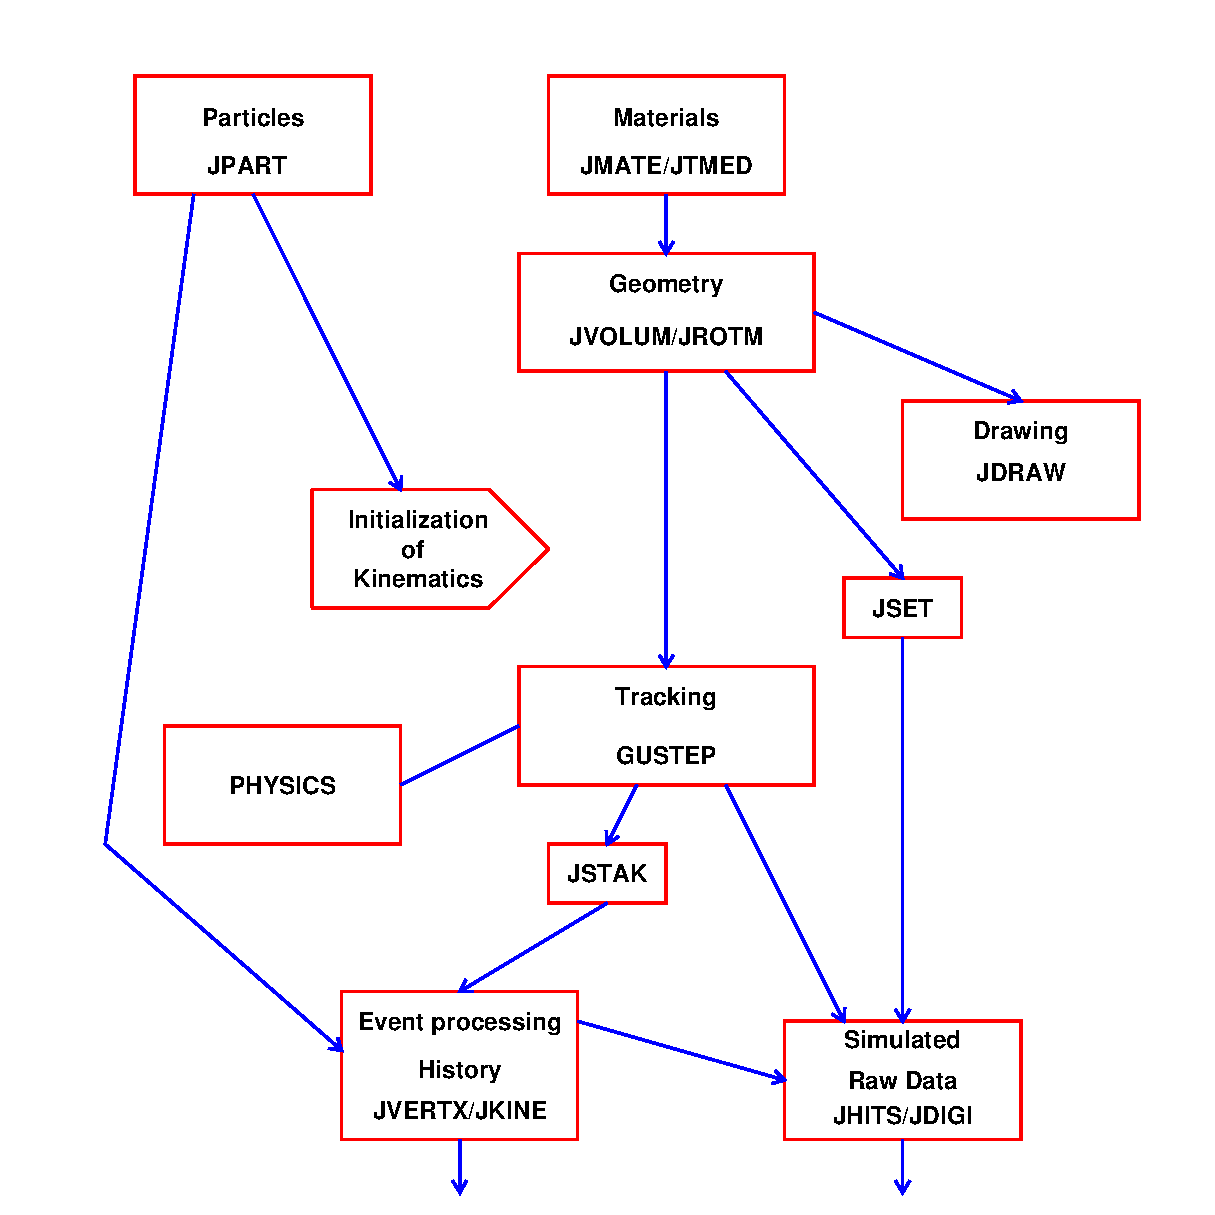
\epsfig{file=eps/base020-1.eps,width=12cm}
     \caption{Relation between {\tt GEANT} data structures}
     \label{fg:base020-1}
\end{figure}
\newpage

\section{Common blocks}
The communication between program segments of the {\tt GEANT} system
is assured by the contents of the data structures and by the definition
of {\it long range} variables in several common blocks.
In addition, within the program segments,
the subroutines communicate with each other through actual arguments
and through the common block variables. A detailed list of the 
user accessed common blocks is given in  {\tt [ZZZZ010]}. 
Their also the variables initialized in \Rind{GINIT} and the possibility
in overriding them through data records {\tt [BASE040]} or 
interactive commands {\tt [XINT]} are specified.
 
In most of the cases there is a correspondence between a
given data structure and a given common block where the current contents of
the banks are stored.
The labelled common blocks are accessible through Patchy/CMZ sequences
identified by the name of the {\tt COMMON}. They are defined in the Patch
\Rind {GCDES}.
 
{\bf Note:}
 
Unless otherwise specified, the long range variables are
initialised in \Rind{GINIT}. When non-zero, default values are
quoted between brackets. If the value may be modified
the keyword for the data record and for the interactive
command is also given in bold characters between brackets.
 

 
 

%%%%%%%%%%%%%%%%%%%%%%%%%%%%%%%%%%%%%%%%%%%%%%%%%%%%%%%%%%%%%%%%%%
%                                                                 %
%  GEANT manual in LaTeX form                                     %
%                                                                 %
%  Version 1.00                                                   %
%                                                                 %
%  Last Mod.  9 June 1993 1300   MG                               %
%                                                                 %
%%%%%%%%%%%%%%%%%%%%%%%%%%%%%%%%%%%%%%%%%%%%%%%%%%%%%%%%%%%%%%%%%%%
\Documentation {F.Bruyant, M.Maire}  
\Submitted {01.10.84}               \Revised{16.12.93}
\Version{Geant 3.16}\Routid{BASE040}
\Makehead{Summary of Data Records}
\section{ Introduction }
 
{\tt GEANT} uses the {\tt FFREAD} \cite{bib-FFREAD}
package to read {\it free format} data records in the routine \Rind{GFFGO}.
The keywords accepted by \Rind{GFFGO} can be
classified as:
\begin{enumerate}
\item         general control of the run;
\item         control of the physics processes;
\item         debug and I/O operations;
\item         user applications;
\item         Lund event generation.
\end{enumerate}
 
The data records are listed below by category with the following information:
\begin{DLtt}{MMMM}
\item[KEY] keyword, any number of characters
truncated to the first 4 unless otherwise specified by the user;
\item[N] maximum expected number of variables ({\tt NVAR});
\item[T] type of these variables ({\tt I=INTEGER, R=REAL or M=MIXED})
and for each variable in turn:
\begin{itemize}
\item variable FORTRAN name;
\item short description (more detail in {\tt [ZZZZ010]});
\item labelled common where it is stored;
\item default value, usually from \Rind{GINIT}.
\end{itemize}
\end{DLtt}
When a record is decoded, the values entered by the user
in free format are assigned to the variables in order.
The number of values can be less than {\tt NVAR}. In case of a {\tt MIXED}
type the values entered have agree
with the type of the corresponding variable.
 
For example the data record:
\begin{verbatim}
      RUNG   5   201
\end{verbatim}
presets the run and event number to 5 and 201 respectively.
None of the records mentioned below is mandatory.
\section{ User defined data records }
 
Before calling \Rind{GFFGO} the user may define private data records
through calls to \Rind{FFKEY} as follows:
\begin{verbatim}
     CALL FFKEY('key',VAR(1),NVAR,'type')
\end{verbatim}
They will be interpreted by \Rind{GFFGO} in the same way as the {\tt GEANT}
pre-defined records.

\section{ Summary of {\tt GEANT} data records }

\subsection{General control}
\begin{tabular}{lllllll}
KEY   &N    &I    &VAR  &\parbox[t]{7.5cm}{Short description}
&\tt COMMON  &\Rind{GINIT} \\
\hline
\tt HSTA  &20 &M &\tt LHSTA &
\parbox[t]{7.5cm}{names of required standard histograms, see {\tt [BASE110]}}
&\FCind{/GCLIST/} & {\tt Blank} \\
\tt OPTI & 1 & I & \tt IOPTI &
\parbox[t]{7.5cm}{automatic optimisation of the geometry via \Rind{GSORD}}
&\FCind{/GCOPTI/} & 1 \\
\tt RNDM  &2  &I & \tt NRNDM & initial random number seed (2 words) &
   \FCind{/GCFLAG/} &0    \\
\tt RUNG  &2  &I & \tt IDRUN & user run number                     &
   \FCind{/GCFLAG/} &1      \\
&     &   &  \tt IDEVT  & first user event number                   &
   \FCind{/GCFLAG/} &1      \\
\tt SORD & 1  &I &\tt ISTORD & stack ordering flag                    &
   \FCind{/GCSTAK/}  & 0 \\
\tt TRIG  &1  &I &\tt NEVENT & total number of events to process      &
   \FCind{/GCFLAG/}  & 10000000\\
\tt TIME  &3  &M &\tt TIMINT &time left after initialisation (see \bf Note
below)
       &
   \FCind{/GCTIME/}  \\
&     &   &  \tt TIMEND &time required for termination        &
  \FCind{/GCTIME/} &1      \\
 
&     &   &  \tt ITIME  &test every {\tt ITIME} events &\FCind{/GCTIME/} &1
\end{tabular}

{\bf Note:} the time allowed for the job after initialisation
cannot be set by the user via the data 
record. To set the total time for the job the user should call the
\Rind{TIMEST} routine at the beginning of the program before any
call to {\tt GEANT} routines. This variable in the 
data record has not been removed for backward compatibility.

\subsection{Control of physics processes}
For more information on the use of these flags, see {\tt [PHYS001]}.

\begin{tabular}{lllllll}
KEY   &N    &I    &VAR  &\parbox[t]{7.5cm}{Short description}
 &\tt COMMON  &\Rind{GINIT} \\
\hline
\tt ANNI  &1  &I &\tt IANNI &annihilation   &\FCind{/GCPHYS/}   &1 \\
\tt AUTO  &1  &I &\tt IGAUTO &\parbox[t]{7.5cm}{automatic computation
of the tracking medium parameters} &\FCind{/GCTRAK/}   &1 \\
\tt BREM  &1  &I &\tt IBREM  &bremsstrahlung &\FCind{/GCPHYS/}  &1 \\
\tt CKOV  &1  &I &\tt ICKOV  &
\v{C}erenkov photon generation &\FCind{/GCTMED/}  &0 \\
\tt COMP  &1  &I &\tt ICOMP  &Compton scattering &\FCind{/GCPHYS/} &1 \\
\tt CUTS  &16 &R &\multicolumn{4}{l}{Kinetic energy cuts in GeV:}      \\
 &    &   &  \tt CUTGAM  &cut for  for gammas    &\FCind{/GCCUTS/} &0.001   \\
 &    &   &  \tt CUTELE  &cut for electrons  &\FCind{/GCCUTS/} &0.001   \\
 &    &   &  \tt CUTNEU  &cut for neutral hadrons&\FCind{/GCCUTS/}&0.01 \\
 &    &   &  \tt CUTHAD  &cut for charged hadrons&\FCind{/GCCUTS/}&0.01  \\
 
 &    &   &  \tt CUTMUO  &cut for muons           &\FCind{/GCCUTS/}&0.01\\
 &    &   &  \tt BCUTE   &cut for electron bremsstrahlung&\FCind{/GCCUTS/}&
    {\tt GUTGAM}\\
 &    &   &  \tt BCUTM   &cut for muon and hadron bremsstrahlung
&\FCind{/GCCUTS/}& \tt CUTGAM\\
 &    &   &  \tt DCUTE   & cut for $\delta$-rays by electrons&\FCind{/GCCUTS/}&
     $10^{4}$\\
&  &  & \tt DCUTM   & cut for $\delta$-rays by muons&\FCind{/GCCUTS/}&$10^{4}$\\
 &    &   &  \tt PPCUTM  & \parbox[t]{7.5cm}{total energy cut for 
direct pair production by muons} &
    \FCind{/GCCUTS/}&0.01\\
 &    &   &  \tt TOFMAX  & time of flight cut in seconds
&\FCind{/GCCUTS/}&$10^{10}$\\
 
 &    &    & \tt GCUTS    &5 user words    &\FCind{/GCCUTS/}&0\\
\tt DCAY  &1   &I&\tt IDCAY    &decay &\FCind{/GCPHYS/}&1\\
\tt DRAY  &1   &I&\tt IDRAY    &$\delta$-ray &\FCind{/GCPHYS/}&1\\
\end{tabular}

\begin{tabular}{lllllll}
KEY   &N    &I    &VAR  &\parbox[t]{7.5cm}{Short description}
 &\tt COMMON  &\Rind{GINIT} \\
\hline
\tt ERAN  &3   &M&\multicolumn{4}{l}{cross-section tables structure:}      \\
 &    &R  &    \tt EKMIN  & minimum energy for the cross-section tables
&\FCind{/GCMULO/}&$10^{-5}$ \\
 &    &R  &    \tt EKMAX  & maximum energy for the cross-section tables
&\FCind{/GCMULO/}&$10^{4}$ \\
 &    &I  &    \tt NEKBIN & \parbox[t]{7.5cm}{number of logarithmic bins 
for cross-section tables}
&\FCind{/GCMULO/}&$90$ \\
\tt HADR  &1   &I&\tt IHADR    &hadronic process &\FCind{/GCPHYS/}&1\\
\tt LABS  &1   &I&\tt ILABS    &\v{C}erenkov light absorbtion 
& \FCind{/GCPHYS/} &0\\
\tt LOSS  &1   &I&\tt ILOSS    &energy loss&
   \FCind{/GCPHYS/} &2\\
\tt MULS  &1   &I&\tt IMULS    &multiple scattering &\FCind{/GCPHYS/}&1\\
\tt MUNU  &1   &I&\tt IMUNU    &muon nuclear interaction
&\FCind{/GCPHYS/}&1\\
\tt PAIR  &1   &I&\tt IPAIR    &pair production &\FCind{/GCPHYS/}&1\\
\tt PFIS  &1   &I&\tt IPFIS    &photofission &\FCind{/GCPHYS/}&0\\
\tt PHOT  &1   &I&\tt IPHOT    &photo electric effect &\FCind{/GCPHYS/}&1\\
\tt RAYL  &1   &I&\tt IRAYL    &Rayleigh scattering &\FCind{/GCPHYS/}&0\\
\tt STRA  &1   &I&\tt ISTRA    &energy fluctuation model&\FCind{/GCPHYS/}&0\\
\tt SYNC  &1   &I&\tt ISYNC    &synchrotron radiation
generation &\FCind{/GCPHYS/}&0\\
\end{tabular}
\subsection{Debug and I/O operations}
\begin{tabular}{lllllll}
KEY   &N    &I    &VAR  &\makebox[7.5cm][l]{Short description}
 &\tt COMMON  &\Rind{GINIT} \\
\hline
\tt DEBU &3 &M &\tt IDEMIN&\parbox[t]{7.5cm}{first event to debug.} 
&\FCind{/GCFLAG/}&0\\
&    &  &  \tt IDEMAX&last event to debug    &\FCind{/GCFLAG/}&0\\
 
&    &  &  \tt ITEST&print control frequency&\FCind{/GCFLAG/}&0\\
\tt GET  &20&M &\tt LGET &\parbox[t]{7.5cm}{
{\tt NGET} names of data structures to
fetch (see \bf Note)}&\FCind{/GCLIST/}& {\tt Blank} \\
\tt PRIN &20 &M & \tt LPRIN&\parbox[t]{7.5cm}{
{\tt NPRIN} user keywords to print data
structure (see \bf Note)}&\FCind{/GCLIST/}& {\tt Blank} \\
\tt RGET  &20&M&\tt LRGET&\parbox[t]{7.5cm}{
{\tt NRGET} names of data structures to fetch
from RZ files (see \bf Note)}&\FCind{/GCRZ/} & {\tt Blank} \\
\tt RSAV &20&M&\tt LRSAVE&\parbox[t]{7.5cm}{
{\tt NRSAVE} names of data structures to save
from RZ files (see \bf Note)}&\FCind{/GCRZ/} & {\tt Blank} \\
\tt SAVE &20&M&\tt LSAVE&\parbox[t]{7.5cm}{
{\tt NSAVE} names of data structures to
save (see \bf Note)}&\FCind{/GCLIST/} & {\tt Blank} \\
\tt SWIT &10&I&\tt ISWIT &user flags for debug&\FCind{/GCFLAG/}&0\\
\end{tabular}

{\bf Note:} the user data records for I/O have no effect on the {\tt GEANT}
system, and the user is supposed to analyse them at run time and take
corresponding action. For instance, a use of the {\tt PRIN} data record
could be the following:
\begin{verbatim}
      CALL GLOOK('VOLU',LPRIN,NPRIN,IPRES)
      IF(IPRES.NE.0) THEN
         CALL GPVOLU(0)
      ENDIF
\end{verbatim}

All the names quoted here are given as 4-character strings in input
and their ASCII equivalent is read into the corresponding variable. The same
applies to the user lists of the following section.

\subsection{User applications}
\begin{tabular}{lllllll}
KEY   &N    &I    &VAR  &\parbox[t]{7.5cm}{Short description}
 &\tt COMMON  &\Rind{GINIT} \\
\hline
\tt KINE  &11   &M    &\tt IKINE   &user flag           &\FCind{/GCKINE/}   &0\\
 
&     &     &     \tt PKINE    &10 user words
    &\FCind{/GCKINE/}    & $10^{10}$\\
\tt SETS  &20   &M    &\tt LSETS    &user words for detector sets
    &\FCind{/GCLIST/}&{\tt Blank}\\
\tt STAT  &20   &M    &\tt LSTAT    &user words to control statistics
&\FCind{/GCLIST/}&{\tt Blank}\\
\tt PLOT  &20   &M    & \tt LPLOT    &user words to control
    plots&\FCind{/GCLIST/}&{\tt Blank}\\
\tt GEOM  &20   &M    &\tt LGEOM    &user words to control geometry
    setup&\FCind{/GCLIST/}&{\tt Blank}\\
\tt VIEW  &20   &M    &\tt LVIEW    &user words to control view banks&
    \FCind{/GCLIST/}&{\tt Blank}\\
\end{tabular}

See note in the previous section on the use of these data records.

\subsection{Lund event generation}
\begin{tabular}{lllllll}
KEY   &N    &I    &VAR  &\makebox[7.5cm][l]{Short description}
 &\tt COMMON  &\Rind{GINIT} \\
\hline
\tt LUND  &2    &M   &\tt IFLUND  &flavour code  (See \FCind{/GLUNDI/})&
\FCind{/GCLUND/}& 0\\
 
&     &     R   &\tt ECLUND  &total CMS energy      &\FCind{/GCLUND/}     &94\\
\end{tabular}

\subsection{Scan geometry control}

The scan geometry has been introduced in {\tt GEANT} version 3.15 with the
idea of developing a general parametrisation scheme. While the scan
geometry can already be built, the parametrisation scheme has not yet
been developed, so the following data records have to be considered as a
{\it forward compatibility} feature.

\begin{tabular}{lllllll}
KEY   &N    &I    &VAR  &\makebox[7.5cm][l]{Short description}
 &\tt COMMON  &\Rind{GINIT} \\
\hline
\tt PCUT &  6 & M & \multicolumn{4}{l}{parametrisation control} \\
& & & \tt IPARAM & parametrisation flag & \FCind{/GCPARM/} & 0 \\
& & & \tt PCUTGA & threshold for gammas & \FCind{/GCPARM/} & 0 \\
& & & \tt PCUTEL & threshold for \Pem\Pep & \FCind{/GCPARM/} & 0 \\
& & & \tt PCUTNE & threshold for neutral hadrons& \FCind{/GCPARM/} & 0 \\
& & & \tt PCUTHA & threshold for charged hadrons & \FCind{/GCPARM/} & 0 \\
& & & \tt PCUTMU & threshold for muons& \FCind{/GCPARM/} & 0 \\
\tt PNUM &  2 & I & \multicolumn{4}{l}{parametrisation stack size} \\
& & & \tt MPSTAK & size of the parametrisation stack & \FCind{/GCPARM/} & 1000 \\
& & & \tt NPGENE & number of pseudo-particles generated & \FCind{/GCPARM/} & 20  \\
\tt SCAN &  8 & M & \multicolumn{4}{l}{scan geometry control} \\
& & & \tt SCANFL & scan processing flag ({\tt LOGICAL}) & \FCind{/GCSCAN/} 
& \tt .FALSE.\\
& & & \tt NPHI &  number of divisions in $\phi$  & \FCind{/GCSCAN/} & 90\\
& & & \tt PHIMIN &  minimum value of $\phi$      & \FCind{/GCSCAN/} &  0\\
& & & \tt PHIMAX &  maximum value of $\phi$      & \FCind{/GCSCAN/} &  360\\
& & & \tt NTETA  &  number of divisions in $\theta$  & \FCind{/GCSCAN/} &  90\\
& & & \tt TETMIN &  minimum value of $\theta$      & \FCind{/GCSCAN/} & 0\\
& & & \tt TETMAX &  maximum value of $\theta$      & \FCind{/GCSCAN/} & 180\\
& & & \tt MODTET &  type of $\theta$ division      & \FCind{/GCSCAN/} &  1\\
\tt SCAL & 32 & M & \tt ISLIST & list of volumes to be {\it scanned} &
\FCind{/GCSCAN/} & \tt Blank \\
\end{tabular}

\begin{tabular}{lllllll}
KEY   &N    &I    &VAR  &\makebox[7.5cm][l]{Short description}
 &\tt COMMON  &\Rind{GINIT} \\
\hline
\tt SCAP &  6 & R & \multicolumn{4}{l}{scan parameters} \\
& & & \tt VX   & scan vertex X coordinate & \FCind{/GCSCAN/} &  0 \\
& & & \tt VY   & scan vertex Y coordinate & \FCind{/GCSCAN/} &  0 \\
& & & \tt VZ   & scan vertex Z coordinate & \FCind{/GCSCAN/} &  0 \\
& & & \tt FACTX0 & scale factor for SX0 & \FCind{/GCSCAN/} &  100 \\
& & & \tt FACTL & scale factor for SL & \FCind{/GCSCAN/} &  1000 \\
& & & \tt FACTR & scale factor for R & \FCind{/GCSCAN/} &  100
\end{tabular}
\subsection{Landau fluctuations versus $\delta$-rays}
In order to avoid double counting between energy loss fluctuations
({\tt ILOSS=2}) and generation of $\delta$-rays {\tt IDRAY=1},
if {\tt ILOSS = 2}
the default value for $\delta$-ray generation is set to {\tt 0} and
it cannot be changed.
The different cases are summarised in the table below.
\begin{center}
\begin{tabular}{|l|l|l|l|}
\hline
                 & Full fluctuations&Restricted fluctuations&No fluctuations \\
                 & \tt ILOSS = 2 (D)   &\tt ILOSS = 1 or 3  & \tt ILOSS = 4 \\
\hline
\tt IDRAY        &\tt 0            &\tt 1          & \tt 1             \\
\tt DCUTE        &\tt 10 TeV       &\tt CUTELE     & \tt CUTELE      \\
\tt DCUTM \quad  &\tt 10 TeV \quad &\tt CUTELE     & \tt CUTELE      \\
\hline
\end{tabular}\end{center}

%%%%%%%%%%%%%%%%%%%%%%%%%%%%%%%%%%%%%%%%%%%%%%%%%%%%%%%%%%%%%%%%%%%
%                                                                 %
%  GEANT manual in LaTeX form                                     %
%                                                                 %
%  Michel Goossens (for translation into LaTeX)                   %
%  Version 1.00                                                   %
%  Last Mod. Jan 24 1991  1300   MG + IB                          %
%                                                                 %
%%%%%%%%%%%%%%%%%%%%%%%%%%%%%%%%%%%%%%%%%%%%%%%%%%%%%%%%%%%%%%%%%%%
\Documentation{R.Brun, F.Bruyant}   
\Submitted{01.10.84}           \Revised{26.10.93}
\Version{Geant 3.16}           \Routid{BASE090}
\Makehead{The reference systems and physical units}
\section{The {\tt MA}ster {\tt R}eference {\tt S}ystem ({\tt MARS})}
 
The kinematic variables of the particles transporter by {\tt GEANT}
are always referred to the so-called 
{\tt MA}ster {\tt R}eference {\tt S}ystem ({\tt MARS}). This system
is implicitly defined as the local reference system of the first
volume defined, which contains all the others. This is a Cartesian
coordinate system with axis $\hat{x}, \hat{y}, \hat{z}$ where
$\hat{z} = \hat{x} \times \hat{y}$.
If the axes are labelled {\tt (X,Y,Z)}, then the point {\tt P}
is represented in fig \ref{fg:base090-1}.
 
\begin{figure}[hbt]
      \centering
      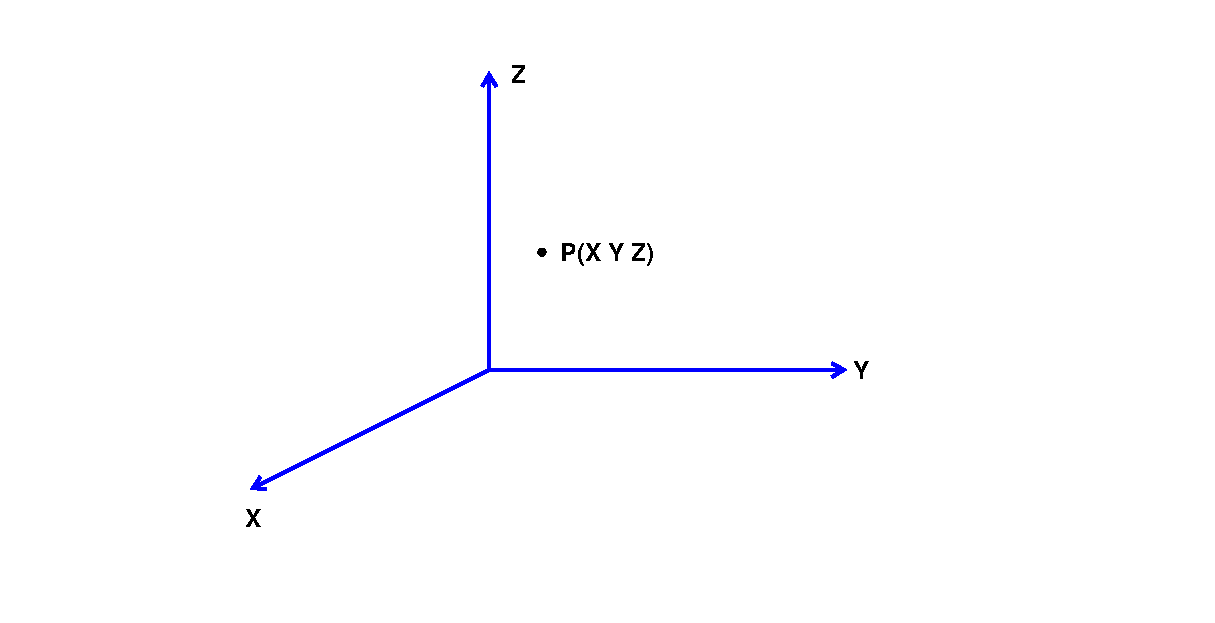
\epsfig{file=eps/base090-1.eps,width=10cm}
      \caption{{\tt GEANT} reference system}
      \label{fg:base090-1}
\end{figure}

Tracking is performed in the {\tt MARS} and the input position for
user routines such as the magnetic field routine is given in this
system.

\section{The local reference systems ({\tt MRS} and {\tt DRS})}
 
As explained in {\tt [GEOM001]}, the setup is
described via the definition of an initial volume inside which all
the others will be positioned. In {\tt GEANT} terminology, each time
a volume has contents, created either via division or by positioning 
other volumes inside, it is called a {\tt MOTHER}. The volumes contained
are called {\tt DAUGHTER}s, and they, in turn, can contain volumes to
a depth of 15 levels. This is sometimes referred to as a {\it Russian doll}
geometry.
 
Every volume defined in {\tt GEANT} has a reference system attached to
it (see {\tt GEOM} section). When this volume has contents, this
is referred to as the {\tt M}other {\tt R}eference {\tt S}ystem
({\tt MRS}, with origin in O$_m$). Daughters
are positioned inside the mother with respect to the {\tt MRS}. The 
{\tt MRS} of the first volume defined, containing all the others, is
nothing else than the {\tt MARS}.

Each one of the daughters has its own reference system, which is referred
to as the {\tt D}aughter {\tt R}eference {\tt S}ystem, or {\tt DRS} with
origin in O$_d$. 

The transformation of a point from the {\tt MRS} (V$_m$)
to the {\tt DRS} (V$_d$), at any level, is performed using a rotation 
matrix $[R]$ and a translation vector $T$ via the relation :
     \[ V_d  =[ R ](V_m -T) \]
The components of $T$ are the projections of the vector  $ (O_m, O_d) $
onto the {\tt MRS} axes.
The rotation matrices are computed from
the spherical angles of each of the axes of the
daughter reference systems ({\tt I, II, III})
with respect to the mother reference system ({\tt 1, 2, 3}).
The spherical angles $\Theta$ and $\Phi$ of a
direction $D$ are defined as follows :
\begin{DLtt}{MMMMM}
\item[$\Theta$]     is the angle formed by the axis 3 and D
                 ($0^{\circ}\;<\;\Theta\;<\;180^{\circ}$).
\item[$\Phi$]      is the angle formed by the axis 1 and the projection
                of D onto the plane defined by the axes 1 and 2
                 ($0^{\circ}\;<\;\Phi\;<\;360^{\circ}$).
\end{DLtt}
Examples are given in {\tt [GEOM200]}.
The various rotation matrices required for a given setup must be
defined by the user during the initialisation stage.
A number is assigned to each matrix {\tt [GEOM200]}.
The translation vector and the number of the rotation
matrix are specified by the user when the volumes are
positioned inside their mother {\tt [GEOM110]}.

\section{Physical units}
 
Unless otherwise specified, the following units are
used throughout the program:
centimeter, second, kilogauss, GeV, GeV c$^{-1}$ (momentum), 
GeV c$^{-2}$ (mass) and degree.

%%%%%%%%%%%%%%%%%%%%%%%%%%%%%%%%%%%%%%%%%%%%%%%%%%%%%%%%%%%%%%%%%%%
%                                                                 %
%  GEANT manual in LaTeX form                                     %
%                                                                 %
%  Michel Goossens (for translation into LaTeX)                   %
%  Version 1.00                                                   %
%  Last Mod. Jan 24 1991  1300   MG + IB                          %
%                                                                 %
%%%%%%%%%%%%%%%%%%%%%%%%%%%%%%%%%%%%%%%%%%%%%%%%%%%%%%%%%%%%%%%%%%%
\Documentation{R.Brun, S.Ravndal}  
\Submitted{01.10.84}    \Revised{10.03.94}
\Version{Geant 3.21}\Routid{BASE100}
\Makehead{Examples of GEANT application}
This section contains a skeleton of a standard user program {\tt GEXAMP}
to use the
{\tt GEANT} system. More detailed examples can be found in the
standard examples {\tt GEXAM1 - 6}. The recommended user routines
are indicated in bold characters and will be explained more in detail
in the following.

\begin{multicols}{2}
\footnotesize
\begin{XMP}
      PROGRAM GEXAMP
      PARAMETER (NGBANK=50000, NHBOOK=5000)
      COMMON/GCBANK/Q(NGBANK)
      COMMON/PAWC  /H(NHBOOK)
C--> {\sl Initialises {\tt HBOOK} and {\tt GEANT} memory}
      CALL GZEBRA( NGBANK)
      CALL HLIMIT(-NHBOOK)
C--> {\sl Open graphics system}
      CALL HPLINT(0)
      CALL IGMETA(8,0)
C--> {\sl {\tt GEANT} initialisation}
      CALL {\bf UGINIT}
C--> {\sl Start events processing}
      CALL GRUN
C--> {\sl End of Run}
      CALL {\bf UGLAST}
      END
*-----------------------------------------------
      SUBROUTINE {\bf UGINIT}
C--> {\sl Initialise {\tt GEANT}}
      CALL GINIT
C--> {\sl Read data records}
      OPEN(4,FILE='gcards.dat',STATUS='UNKNOWN')
      CALL GFFGO
C--> {\sl Initialise data structure}
      CALL GZINIT
C--> {\sl Initialise graphics}
      CALL GDINIT
      IF(NRGET.GT.0) THEN
C--> {\sl Read data structures from file}
         CALL GRFILE(1,'mygeom.dat','I')
      ELSE
C--> {\sl Particle table initialisation}
         CALL GPART
C--> {\sl Geometry and materials description}
         CALL UGEOM
      ENDIF
C--> {\sl Energy loss and cross-sections tables}
      CALL GPHYSI
      IF(NRSAVE .GT. 0) THEN
C--> {\sl Save permanent data structures} 
         CALL GRFILE(2,'mysave.dat','NO')
      ENDIF
C--> {\sl Print banks}
      CALL GPRINT('MATE',0)
      CALL GPRINT('TMED',0)
      CALL GPRINT('VOLU',0)
C--> {\sl Book histograms} 
      END
*-----------------------------------------------
      SUBROUTINE {\bf UGEOM}
C--> {\sl Defines material, tracking media }
C--> {\sl and geometry.}
C--> {\sl Close geometry banks.}
      CALL GGCLOS
      END
*-----------------------------------------------
      SUBROUTINE {\bf GUKINE}
C--> {\sl Generates kinematics}
C--> {\sl Data card {\tt KINE} itype x y z px py pz}
+SEQ, GCFLAG.
+SEQ, GCKINE.
      CALL GSVERT(PKINE,0,0,0,0,NVERT)
      CALL GSKINE(PKINE(4),IKINE,NVERT,0,0,NT)
C--> {\sl Print kinematic}
      IF (IDEBUG.NE.0) THEN
         CALL GPRINT('VERT',0)
         CALL GPRINT('KINE',0)
      END IF
      END
*-----------------------------------------------
      SUBROUTINE {\bf GUSTEP}
C--> {\sl Called at the end of each tracking }
C--> {\sl step.}
+SEQ, GCKINE.
C--> {\sl Debug event}
      CALL GDEBUG
C--> {\sl Store the created particles} 
      IF (NGKINE.GT.0) CALL GSKING (0)
      END
*-----------------------------------------------
      SUBROUTINE {\bf UGLAST}
C--> {\sl Termination routine} 
C--> {\sl Print histograms and statistics}
      CALL GLAST
C--> {\sl Close {\tt HIGZ/GKS} file}
      CALL IGEND
      END
\end{XMP}
\end{multicols}

\section{Notes}
\begin{itemize}
\item Whenever possible {\tt GEANT} makes use of the {\tt ZEBRA} store
for large data structures. This allows it to adapt the size of the program
data portion
to the size of the problem. The total amount of space required depends
on the application. {\tt GEANT} can run with as little as 50,000 words
or less, but for large detectors it is not uncommon to 
declare stores of several million words. The call to \Rind{GZEBRA}
initialises the common \FCind{/GCBANK/} to receive the {\tt GEANT}
data structures. This call is necessary before any other routine of
the {\tt GEANT} system is called.
\item The call to \Rind{HLIMIT} initialises the {\tt ZEBRA} system
to use the \FCind{/PAWC/} common block for the {\tt HBOOK} histogram
package. The size of the common depends on the number and size of the
plot requested. The {\tt ZEBRA} system must be initialised only once,
and the negative argument to \Rind{HLIMIT} prevents a second
initialisation of the system.
The \Rind{HLIMIT} call has to be placed {\bf after} the call
to \Rind{GZEBRA} and the argument has to be the dimension of the 
\FCind{/PAWC/} common block with a negative sign in front. 
\item
The main program is intended for {\it batch} applications,
while to run the simulation interactively, the interactive main program
called \Rind{GXINT} should be linked in front of the user code.
\item The program shown will require the graphic libraries in the
link sequence. Often, for batch production or for
small tests, graphics is not needed, and not loading the graphics
code makes the program smaller. To avoid loading graphic routines
the calls to \Rind{IGINIT}, \Rind{IGMETA}, \Rind{IGEND}, \Rind{GDINIT}
and \Rind{GDEBUG} should be removed. 

If, on the other hand, the user is interested in including the routine
\Rind{GDEBUG} and in excluding graphics at the same time, then the
following routine should be included in the code:
\begin{verbatim}
      SUBROUTINE GDCXYZ
      ENTRY IGSA
      ENTRY GDTRAK
      END
\end{verbatim}

which will avoid every reference to the graphics routines from \Rind{GDEBUG}.

\item The user code to define the {\it tracking media} and the geometry
of the setup should be inside the routine \Rind{UGEOM}. The pre-initialised
data structured can be read from disk, but it is recommended to call 
\Rind{GPHYSI} in any case, to initialise the cross-section tables. An 
example of a full material, geometry and detector design is given below
and has been extracted from the example {\tt GEXAM3}. Here only major
calls are shown, the redundant parts can be found in the source code
of \Rind{UGEOM} in {\tt GEXAM3}. 

The example shows the basic concept in 
{\tt GEANT}. First material parameters are defining the properities of
a detector material calling the subroutine \Rind{GSMATE}. 
Here in addition to the 16 predefined materials, the material definition of
Calcium is examplary shown. More information towards the predefined materials
and further use of material definition routines can be found in the 
section {\tt CONS001 - CONS101}.
Then tracking parameters are associated to the materials, defining
a so called tracking medium. Each {\tt GEANT}  volume must be 
associated to an existing tracking medium. Here in the example the
tracking medium {\tt 'TARGET'} is defined to exist of Calcium.
 
In the example shown below several
detector volumes are defined using the subroutine \Rind{GSVOLU}.
The defined volume have associated parameters of name, shape,
tracking medium and shape parameters.
In this example the volume {\tt 'TGT '} consists of the 
previously defined tracking medium {\tt 'TARGET'}.The 
volumes (and if necessary identical copies of them)
are then positioned according to the detector geometry. The 
volumes are positioned on the same level, or inside each other. By
setting the parameter {\tt ONLY} or  {\tt MANY} in the call of \Rind{GSPOS} 
the user has the opportunity to tell either {\tt GEANT} the logical
volume structure and to apply boolean operations (cutting, joining and
intersection) between two positioned volumes. More information about
the concept in defining volumes and positioning can be retrieved from
the section {\tt GEOM}. 

Finally the user is required to classify into sets all
sensitive detectors (defined as those volume defined as
detector via \Rind{GSDET} and other related routines, for which 
he wants to store hits in the hit data structure {\tt JHITS}.
\begin{multicols}{2}
\footnotesize
\begin{XMP}
      SUBROUTINE {\bf UGEOM}
+SEQ,GCLIST
+SEQ,GCONSP
      COMMON/DLSFLD/ISWFLD,FLDVAL
C--> {\sl Defining material parameters}
C--> {\sl Defining geometry parameters}
C--> {\sl Defining positioning parameters}
C--> {\sl Data statements, left out here, to}
C--> {\sl Define materials and mixtures}
      CALL GSMATE(17,'CALCIUM$',
     + 40.08,20.,1.55,10.4,23.2,0,0)
C--> {\sl .......}
C--> {\sl further material an mixture definitions}
C--> {\sl .......}
C--> {\sl Defining tracking media}
      CALL GSTMED( 2,'TARGET    $',
     + 17,0,0,0.,10.,.2,.1,.001,.5,0,0)
C--> {\sl .......}
C--> {\sl defining further media}
C--> {\sl .......}
C--> {\sl Define the reference frame}
      CALL GSVOLU
     +     ('CAVE','BOX ',1,CAVPAR,3,ICAVE)
C--> {\sl The targe box is shifted by 100 cm}
C--> {\sl in the cave.}
      CALL GSVOLU
     +     ('TGT ','BOX ',2,TGTPAR,3,ITGT )
      CALL GSVOLU
     +     ('TBIN','TRD1',3,TBIPAR,4,ITBIN)
      CALL GSVOLU
     +     ('TBOU','TRD1',4,TBOPAR,4,ITBOU)
      CALL GSVOLU
     +     ('ARM ','TRD1',1,ARMPAR,4,IARM)
      CALL GSVOLU
     +     ('FDIN','BOX ',9,FDIPAR,3,IFDIN)
      CALL GSVOLU
     +     ('FDOU','BOX ',4,FDOPAR,3,IFDOU)
C--> {\sl Define drift wire planes}
      CALL GSVOLU
     +     ('FSP ','BOX ',13,FDIPAR,3,IFSP)
C--> {\sl .......}
C--> {\sl further geometry definitions}
C--> {\sl .......}
C--> {\sl Positioning the daughter volumes in}
C--> {\sl their mother volume.}
      CALL GSPOS
     + ('TGT ',1,'TBIN', 0., 0.,-5.08,0,'ONLY')
      CALL GSPOS
     + ('TGT ',2,'TBIN', 0., 0.,-2.54,0,'ONLY')
      CALL GSPOS
     + ('TGT ',3,'TBIN', 0., 0., 0.  ,0,'ONLY')
      CALL GSPOS
     + ('TGT ',4,'TBIN', 0., 0., 2.54,0,'ONLY')
      CALL GSPOS
     + ('TGT ',5,'TBIN', 0., 0., 5.08,0,'ONLY')
      CALL GSPOS
     + ('TBIN',1,'TBOU', 0., 0.,   0.,0,'ONLY')
      CALL GSPOS
     + ('TBOU',1,'CAVE', 0., 0.,  ZTG,0,'ONLY')
      CALL GSPOS
     + ('ARM ',1,'CAVE',XLARM,0.,ZLARM,1,'ONLY')
      CALL GSPOS
     + ('ARM ',2,'CAVE',XRARM,0.,ZRARM,2,'ONLY')
      CALL GSPOS
     + ('FDOU',1,'ARM ',0.,0., DFDO  ,0,'ONLY')
      CALL GSPOS
     + ('FDIN',1,'FDOU',0.,0., 0.    ,0,'ONLY')
      CALL GSPOS
     + ('FSP ',1,'FDIN',0.,0.,-2.9975,0,'ONLY')
C--> {\sl .......}
C--> {\sl positioning of further volumes}
C--> {\sl .......}
C--> {\sl Print the stored definitions}
      CALL GLOOK('VOLU',LPRIN,NPRIN,ILOOK)
      IF(ILOOK.NE.0) CALL GPVOLU(0)
      CALL GLOOK('ROTM',LPRIN,NPRIN,ILOOK)
      IF(ILOOK.NE.0) CALL GPROTM(0)
      CALL GLOOK('TMED',LPRIN,NPRIN,ILOOK)
      IF(ILOOK.NE.0) CALL GPTMED(0)
      CALL GLOOK('MATE',LPRIN,NPRIN,ILOOK)
      IF(ILOOK.NE.0) CALL GPMATE(0)
      CALL GLOOK('PART',LPRIN,NPRIN,ILOOK)
      IF(ILOOK.NE.0) CALL GPPART(0)
C--> {\sl Clean up volume banks and perform}
C--> {\sl optimization}
      CALL GGCLOS
C--> {\sl Define sensitive detector parts}
      CALL GSDET
     &('DRFT','FSP ',2,NAFD ,NBITSV,1,100,
     &100,IDRFT,IFD )
C--> {\sl Define hit parameters}
      CALL GSDETH('DRFT','FSP ',9,NAMESH,
     &NBITSH,ORIG,FACT)
      RETURN
      END
\end{XMP}
\end{multicols}





\item It is convenient to store the input data records (see {\tt [BASE040]})
in an auxiliary file ({\tt gcards.dat} in the example). This allows to
have a standard input file and to overwrite selected input data records
as needed.
If, for instance, the standard {\tt gcards.dat} file contains the record
{\tt TRIG 1000} and a short test run is requested this can be obtained
with the following input:
\begin{verbatim}
READ 4
TRIG 10
STOP
\end{verbatim}
the first line instructs {\tt FFREAD} to open and process the file
connected with logical unit 4, and the second line (re-)defines the
number of events to be processed. The {\tt STOP} command ends the 
{\tt FFREAD} processing of the input.
\item 
In the above
example the common blocks have not been expanded in the code. The notation
used is the one of the {\tt PATCHY}/{\tt CMZ}~\cite{bib-PATCHY,bib-CMZ}
code management systems. These products, among other things, can
run as pre-processors, replacing the {\tt +SEQ,...}
instructions with the corresponding code fragments. Users are strongly
recommended to use these systems to include {\tt GEANT} common blocks
in their code. 

Long experience in supporting {\tt GEANT} users has shown that, as the
user program grows, typing errors in the insertion of the common blocks
{\it by hand} become very common, but difficult to find. The investment
needed to learn a code management system at the user level is usually 
negligible compared with the time and energy needed in hunting a
problem introduced by a mistyped common.
\end{itemize}

%%%%%%%%%%%%%%%%%%%%%%%%%%%%%%%%%%%%%%%%%%%%%%%%%%%%%%%%%%%%%%%%%%%
%                                                                 %
%  GEANT manual in LaTeX form                                     %
%                                                                 %
%  Version 1.00                                                   %
%  Last Mod.  8 June 1993 1300   MG                               %
%                                                                 %
%%%%%%%%%%%%%%%%%%%%%%%%%%%%%%%%%%%%%%%%%%%%%%%%%%%%%%%%%%%%%%%%%%%
\Origin {R.Brun} 
\Submitted{01.06.83}  \Revised{16.12.93}
\Version{Geant 3.16}\Routid{BASE110}
\Makehead{The system initialisation routines}
 
\Shubr{GZEBRA}{(NZ)}
 
Initialises the {\tt ZEBRA} memory manager to use the common \FCind{/GCBANK/}
to store the {\tt GEANT} data structures.
\begin{DLtt}{MMMMMMMM}
\item[NZ] ({\tt INTEGER}) size of the \FCind{/GCBANK/} common as it is
dimensioned in the main program.
\end{DLtt}
The size of the dynamic memory is set to {\tt NZ-30}. The common
\FCind{/GCBANK/} must be dimensioned in the main program.
{\tt ZEBRA}~\cite{bib-ZEBRA} must be initialised only once. The call to the
{\tt HBOOK} initialisation routine \Rind{HLIMIT} tries to initialise
{\tt ZEBRA} as well, and this will cause a program abort. To avoid this,
\Rind{HLIMIT} must be called {\bf after} \Rind{GZEBRA} and its argument
must be a negative number whose absolute value is the size of the
\FCind{/PAWC/} common containing the histograms. This is shown in the
example of main program given in {\tt[BASE100]}.

\Shubr{GINIT}{}
Presets labelled common block variables to default values.
See {\tt[BASE030]} for more information.

\Shubr{GFFGO}{}
Reads a set of data records via the {\tt FFREAD} package.
See {\tt[BASE040]} for more information on the possible data records.
\Rind{GFFGO} must be called after \Rind{GINIT}.

\Shubr{GZINIT}{}

Initialises the {\tt ZEBRA} permanent data structures in division
2 of the {\tt GEANT} main store in common  \FCind{/GCBANK/}.
Creates the user long term division (index {\tt IXCONS})
(minimum size {\tt 2000}, maximum size {\tt 8*NZEBRA/10}).
The {\tt ZEBRA} division {\tt IXDIV} is reserved for the event data structures
and the division {\tt IXCONS} for the initialisation data structures.
Allocates 5200 words of working space.
Initialises the link areas and a default run header bank {\tt JRUNG
[BASE299]}. Defines banks format for I/O.
\Rind{GZINIT} must be called after \Rind{GFFGO}.
 
A layout of the dynamic store is shown in fig \ref{fg:base110-1}.

\begin{figure}[hbt]
      \centering
      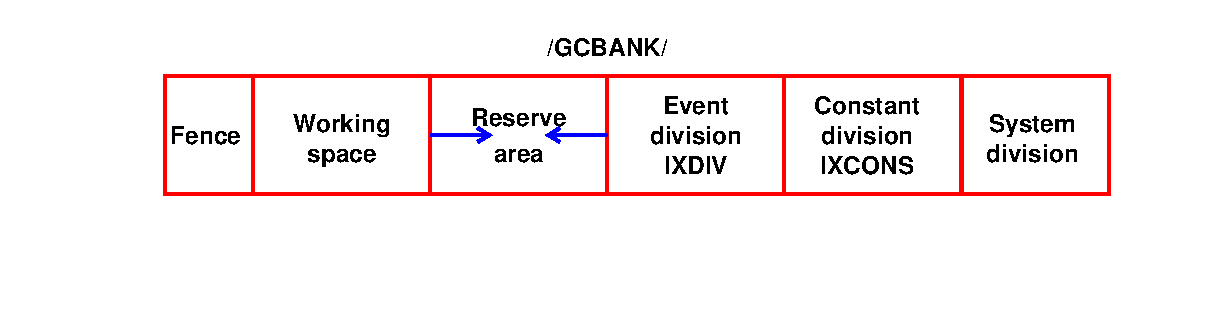
\epsfig{file=eps/base110-1.eps,width=16cm}
      \caption{Layout of the dynamic store}
      \label{fg:base110-1}
\end{figure}

\Shubr{GDINIT}{}
This routine
initialises the {\tt GEANT} drawing package {\tt[DRAW001]} and it has
to be called before any other graphic routine. {\tt GEANT} uses the
CERN-developed {\tt HIGZ}~\cite{bib-HIGZ} graphic library, and this
has to be initialised before the call to \Rind{GDINIT}.
In the example given
in {\tt [BASE100]} the routines \Rind{IGINIT} and \Rind{IGMETA}
are used. Alternatively, the routine \Rind{HPLINT} from HPLOT~\cite{bib-HPLOT}
can be used. This routine calls the appropriate procedures from {\tt HIGZ} to 
initialise the underlaying graphics system. At the moment {\tt HIGZ} can 
use several flavours of GKS~\cite{bib-gks2d,bib-gks3d,bib-GKS1}
and {\tt X11} and it is available on all machines where the CERN Program
Library has been installed.

\Shubr{GPHYSI}{}
Completes the data structure {\tt JMATE}, (see {\tt [PHYS100]}) calculating the
cross-section and stopping power tables.

\Shubr{GBHSTA}{}
Initialises the standard histograms requested by the user via the
data record {\tt HSTA}.
The following histogram keywords may be used :
\begin{DLtt}{MMMMMMMM}
\item[TIME]    time per event;
\item[SIZE]     size of division {\tt IXDIV} per event;
\item[MULT]    total number of tracks per event;
\item[NTRA]    number of {\it long life} tracks per event;
\item[STAK]    maximum stack size per event.
\end{DLtt}

\Rind{GBHSTA} should be called after \Rind{GFFGO}.

\Shubr{GGCLOS}{}
This routine has to be called at the end of the definition
of the geometry by the user, after thal all volumes have been defined
and positioned and all detectors defined. 
Failure to call this routine will prevent
the {\tt GEANT} system from working correctly. Main tasks of this routine
are:
\begin{itemize}
\item close the geometry package;
\item complete the {\tt JVOLUM} data structure;
\item process the detector definition provided by the user;
\item prepare the tables for the tracking speed optimisation requested
by the user via the \Rind{GSORD} routine or the {\tt OPTI} data record.
\end{itemize}

%%%%%%%%%%%%%%%%%%%%%%%%%%%%%%%%%%%%%%%%%%%%%%%%%%%%%%%%%%%%%%%%%%%
%                                                                 %
%  GEANT manual in LaTeX form                                     %
%                                                                 %
%  Version 1.00                                                   %
%  Last Mod.  8 June 1993 1300   MG                               %
%                                                                 %
%%%%%%%%%%%%%%%%%%%%%%%%%%%%%%%%%%%%%%%%%%%%%%%%%%%%%%%%%%%%%%%%%%%
\Origin{R.Brun}     
\Submitted{01.06.83}   \Revised{26.10.93}
\Version{Geant 3.16}\Routid{BASE200}
\Makehead{Steering routines for event processing}
\Shubr{GRUN}{}
Main routine to control a run of events. The following flow chart is only 
valid for the {\it batch} execution mode. For interactive applications, 
see section {\tt XINT}. A schematic description of the routine is shown 
in fig.~\ref{fg:base200-1}.
 
\begin{figure}[hbt]
      \centering
      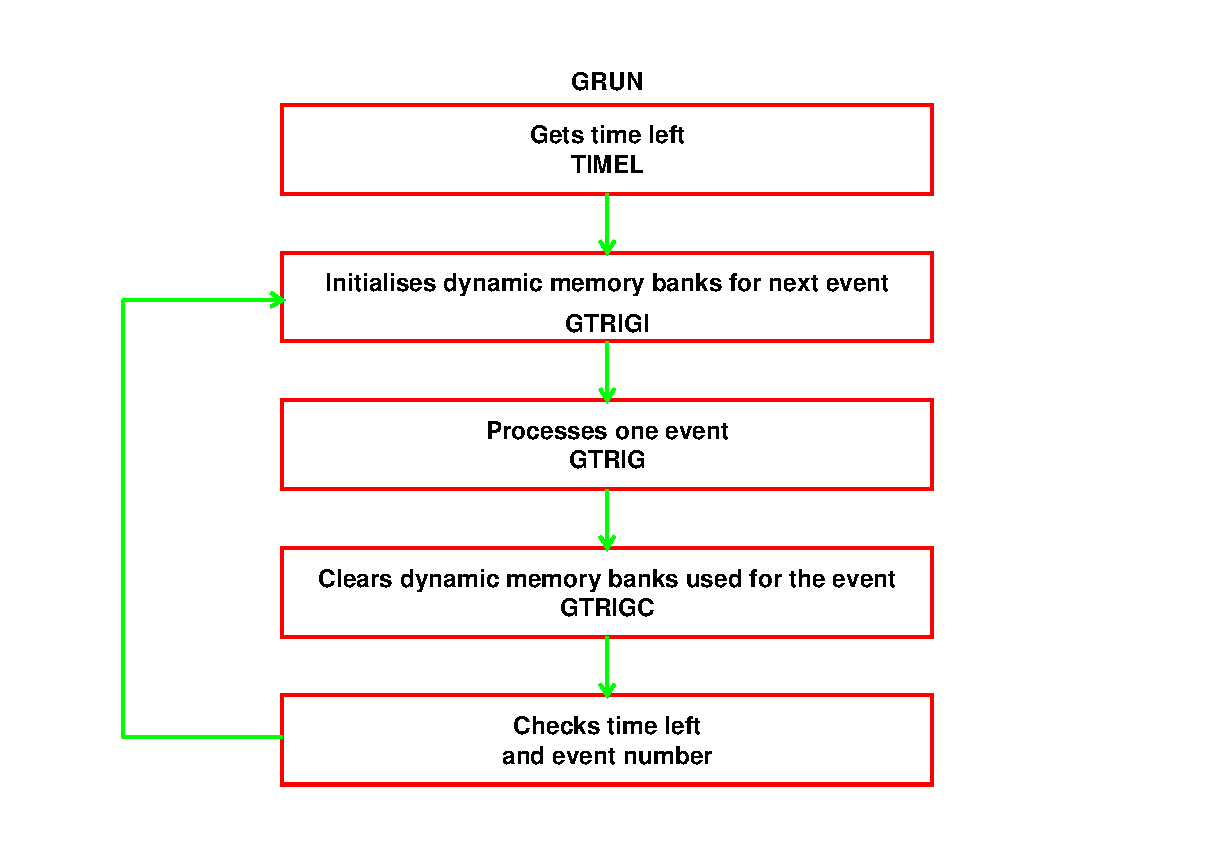
\epsfig{file=eps/base200-1.eps,width=16cm}
      \caption{Flow of the {\tt GRUN} routine.}
      \label{fg:base200-1}
\end{figure}

\Shubr{GTRIGI}{}
Initialisation routine for event processing:
\begin{itemize}
\item resets to 0 the flag {\tt IEOTRI} in \FCind{/GCFLAG/} and the counters
{\tt NTRACK} and {\tt NVERTX} in \FCind{/GCNUM/};
\item sets the debug flag
{\tt IDEBUG} in \FCind{/GCFLAG/}
to the value required for the current event;
\item creates a default header bank
{\tt JHEAD} for current event {\tt [BASE299]};
\item prints the sequence number, the event number and the random number
generator seeds,
under control of the flag {\tt ITEST} (data record {\tt DEBU}).
\end{itemize}
 
\Shubr{GTRIG}{}
 
Steering routine to process one event (trigger).
A schematic description of the routine is shown 
in fig.~\ref{fg:base200-2}.
 
\begin{figure}[hbt]
      \centering
      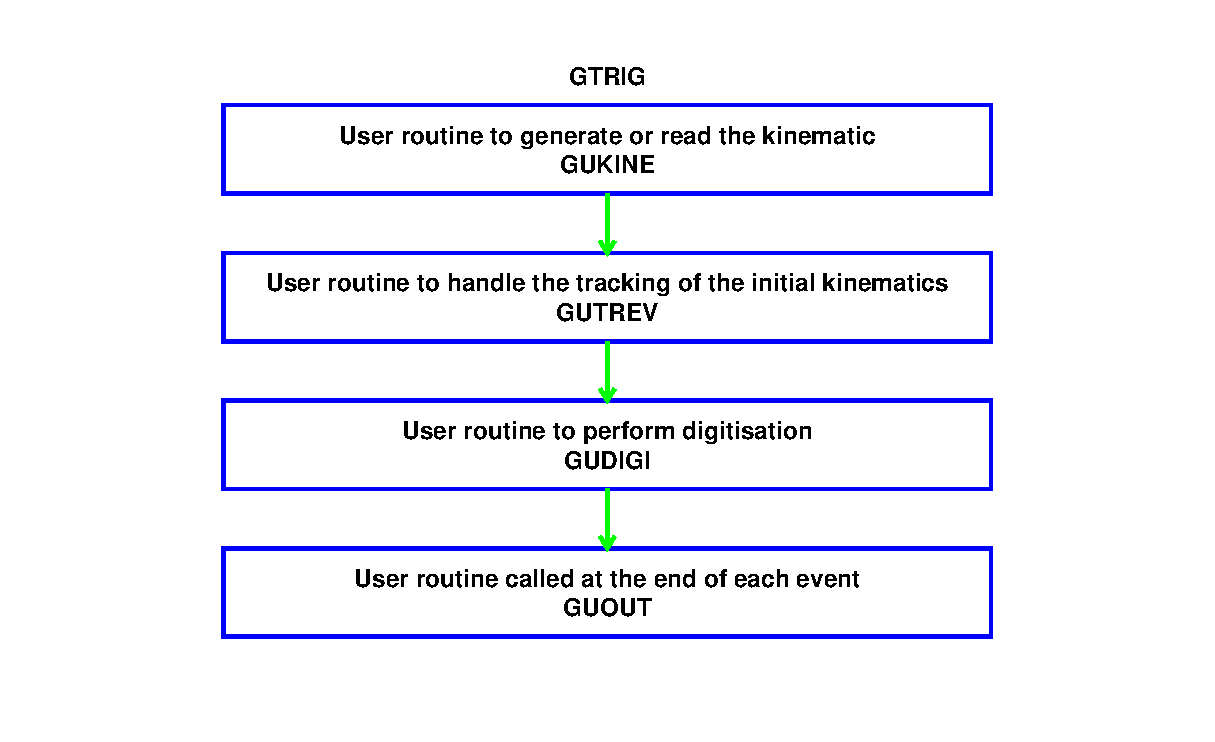
\epsfig{file=eps/base200-2.eps,width=16cm}
      \caption{Flow of the {\tt GRUN} routine.}
      \label{fg:base200-2}
\end{figure}

Default routines provided by {\tt GEANT} are dummy.

\Shubr{GTRIGC}{}
The event division {\tt IXDIV} is cleared. The space
used by the current event may be used by the next one.
 

%%%%%%%%%%%%%%%%%%%%%%%%%%%%%%%%%%%%%%%%%%%%%%%%%%%%%%%%%%%%%%%%%%%
%                                                                 %
%  GEANT manual in LaTeX form                                     %
%                                                                 %
%  Michel Goossens (for translation into LaTeX)                   %
%  Version 1.00                                                   %
%  Last Mod. Jan 24 1991  1300   MG + IB                          %
%                                                                 %
%%%%%%%%%%%%%%%%%%%%%%%%%%%%%%%%%%%%%%%%%%%%%%%%%%%%%%%%%%%%%%%%%%%
\Origin{M.Maire}
\Submitted{14.12.93}  \Revised{14.12.93}
\Version{Geant 3.16}\Routid{BASE280}

\Makehead{Storing and retrieving JRUNG and JHEAD information}

\Shubr{GSRUNG}{(NUBUF,UBUF,IADR*)}
\begin{DLtt}{MMMMMMMM}
\item[NUBUF] ({\tt INTEGER}) number of user words;
\item[UBUF] ({\tt REAL}) array of user words;
\item[IADR] ({\tt INTEGER}) position where information is stored in the
user bank of the {\tt JRUNG} structure.
\end{DLtt}

This routine stores the first {\tt NUBUF} words of array {\tt BUF} in the
user bank attached to the structure {\tt JRUNG} (see {\tt [BASE299]}),
starting at location {\tt IADR+1}.
On exit {\tt IADR} is set to {\tt IADR+NUBUF}, allowing subsequent filling. 
This allows effectively 
to {\it add} information to the current {\tt JRUNG} bank, whether or not it has 
already an user buffer.

\Shubr{GFRUNG}{(NWRUNG*,IRUNG*,NUBUF*,UBUF*)}
\begin{DLtt}{MMMMMMMM}
\item[NWRUNG] ({\tt INTEGER}) number of words in {\tt JRUNG} bank;
\item[IRUNG] ({\tt REAL}) content of {\tt JRUNG} bank;
\item[NUBUF] ({\tt INTEGER}) number of user words;
\item[UBUF] ({\tt REAL}) array of user words;
\end{DLtt}

This routine retrieves the content of the {\tt JRUNG} bank and of the
user information added, if any.

\Shubr{GPRUNG}{}

This routine prints the content of the {\tt JRUNG} bank and of the
user information added, if any.

\Shubr{GSHEAD}{(NUBUF,UBUF,IADR*)}
\begin{DLtt}{MMMMMMMM}
\item[NUBUF] ({\tt INTEGER}) number of user words;
\item[UBUF] ({\tt REAL}) array of user words;
\item[IADR] ({\tt INTEGER}) position where information is stored in the
user bank of the {\tt JHEAD} structure.
\end{DLtt}

This routine stores the first {\tt NUBUF} words of array {\tt BUF} in the
user bank attached to the structure {\tt JHEAD} (see {\tt [BASE299]}),
starting at location {\tt IADR+1}.
On exit {\tt IADR} is set to {\tt IADR+NUBUF}, allowing subsequent filling. 
This allows effectively 
to {\it add} information to the current {\tt JHEAD} bank, whether or not it has 
already an user buffer.

\Shubr{GFHEAD}{(NWHEAD*,IHEAD*,NUBUF*,UBUF*)}
\begin{DLtt}{MMMMMMMM}
\item[NWHEAD] ({\tt INTEGER}) number of words in {\tt JHEAD} bank;
\item[IHEAD] ({\tt REAL}) content of {\tt JHEAD} bank;
\item[NUBUF] ({\tt INTEGER}) number of user words;
\item[UBUF] ({\tt REAL}) array of user words;
\end{DLtt}

This routine retrieves the content of the {\tt JHEAD} bank and of the
user information added, if any.

\Shubr{GPHEAD}{}

This routine prints the content of the {\tt JHEAD} bank and of the
user information added, if any.

%%%%%%%%%%%%%%%%%%%%%%%%%%%%%%%%%%%%%%%%%%%%%%%%%%%%%%%%%%%%%%%%%%%
%                                                                 %
%  GEANT manual in LaTeX form                                     %
%                                                                 %
%  Michel Goossens (for translation into LaTeX)                   %
%  Version 1.00                                                   %
%  Last Mod. Jan 24 1991  1300   MG + IB                          %
%                                                                 %
%%%%%%%%%%%%%%%%%%%%%%%%%%%%%%%%%%%%%%%%%%%%%%%%%%%%%%%%%%%%%%%%%%%
\Origin{R.Brun, F.Bruyant}  
\Submitted{01.10.84}  \Revised{14.12.93}
\Version{Geant 3.16}\Routid{BASE299}
\Makehead{The banks JRUNG and JHEAD}
Run bank {\tt JRUNG}:  1 user link, 30 data words
 
\vspace{0.7cm}
\begin{tabular}{r@{}ll}
\hspace{2cm} {\tt LQ(JRUNG} &{\tt-1)} &user link      \\
                                                      \\
{\tt IQ(JRUNG}&{\tt+1)} &{\tt IDRUN} (Run number)           \\
&{\tt+2 \dots +10)} &Reserved for user applications    \\
&{\tt+11)} &creation date for {\tt INIT} data structures \\
&{\tt+12)} &creation time for {\tt INIT} data structures \\
&{\tt+13)} &creation date for {\tt KINE}                 \\
&{\tt+14)} &creation time for {\tt KINE}                 \\
&{\tt+15)} &creation date for {\tt HITS}                 \\
&{\tt+16)} &creation time for {\tt HITS}                 \\
&{\tt+17)} &creation date for {\tt DIGI}                 \\
&{\tt+18)} &creation time for {\tt DIGI}                 \\
&{\tt+19)} &\parbox[t]{10cm}{{\tt NRNDM(1)}
First seed for the random number generator 
at the end of the last event generated}\\
&{\tt+20)} &\parbox[t]{10cm}{{\tt NRNDM(2)}
Second seed for the random number generator 
at the end of the last event generated}\\
&{\tt+21)} &{\tt GEANT} version number when {\tt INIT} created  \\
&{\tt+22)} &{\tt ZEBRA} version number when {\tt INIT} created  \\
&{\tt+23)} &{\tt GEANT} version number when {\tt KINE} created  \\
&{\tt+24)} &{\tt ZEBRA} version number when {\tt KINE} created  \\
&{\tt+25)} &{\tt GEANT} version number when {\tt HITS} created  \\
&{\tt+26)} &{\tt ZEBRA} version number when {\tt HITS} created  \\
&{\tt+27)} &{\tt GEANT} version number when {\tt DIGI} created  \\
&{\tt+28)} &{\tt ZEBRA} version number when {\tt DIGI} created  \\
&{\tt+29)} &\parbox[t]{10cm}{{\tt IEVENT} event sequence number 
at the end of the last generated event} \\
\end{tabular}
\vspace{0.7cm}
 
Header bank {\tt JHEAD}: 1 user link, {\tt NHEAD(=10)} data words
\vspace{0.7cm}
 
\begin{tabular}{r@{}lll}
\hspace{2cm} {\tt LQ(JHEAD} &{\tt-1)} &user link      \\
                                                       \\
{\tt IQ(JHEAD}&{\tt+1)} &{\tt IDRUN} &Run number         \\
&{\tt+2)} &{\tt IDEVT} &Event number                  \\
&{\tt+3)} &{\tt NRNDM(1)} &\parbox[t]{8.1cm}{Value of random number generator 
first seed at the beginning of the event} \\
&{\tt+4)} &{\tt NRNDM(2)} &\parbox[t]{8.1cm}{Value of random number generator 
second seed at the beginning of the event} \\
&{\tt+5 \dots 10)} & & Reserved for user applications         \\
\end{tabular}

%%%%%%%%%%%%%%%%%%%%%%%%%%%%%%%%%%%%%%%%%%%%%%%%%%%%%%%%%%%%%%%%%%%
%                                                                 %
%  GEANT manual in LaTeX form                                     %
%                                                                 %
%  Version 1.00                                                   %
%  Last Mod.  8 June 1993 1300   MG                               %
%                                                                 %
%%%%%%%%%%%%%%%%%%%%%%%%%%%%%%%%%%%%%%%%%%%%%%%%%%%%%%%%%%%%%%%%%%%
\Documentation{R.Brun}  
\Submitted{01.10.84} \Revised{08.11.93}
\Version{Geant 3.16}\Routid{BASE300}
\Makehead{Example of user termination routine}
\begin{verbatim}
    SUBROUTINE UGLAST
*
+SEQ,GCLIST
*
*       Call standard GEANT termination routine
    CALL GLAST
*
*       Terminate graphics
    CALL HPLEND
*
*       Close I/O buffers
    IF(NGET .NE. 0 .OR. NSAVE .NE. 0) CALL GCLOSE(0,IER)
*
*       Print histograms
    CALL HISTDO
*
    END
\end{verbatim}
\Shubr{GLAST}{}
Standard {\tt GEANT} termination routine:
\begin{itemize}
\item computes and prints the processing time per event;
\item calls \Rind{MZEND} to print the statistics relative to the current run;
\item if the structure {\tt JGSTAT} has been initialised, calls \Rind{GPSTAT}
{\tt [GEOM700]}.
\end{itemize}

%%%%%%%%%%%%%%%%%%%%%%%%%%%%%%%%%%%%%%%%%%%%%%%%%%%%%%%%%%%%%%%%%%%
%                                                                 %
%  GEANT manual in LaTeX form                                     %
%                                                                 %
%  Version 1.00                                                   %
%  Last Mod.  8 June 1993 1300   MG                               %
%                                                                 %
%%%%%%%%%%%%%%%%%%%%%%%%%%%%%%%%%%%%%%%%%%%%%%%%%%%%%%%%%%%%%%%%%%%
\Origin{R.Brun, F.Carena}
\Submitted{01.10.84}  \Revised{16.12.93}
\Version{Geant 3.16}\Routid{BASE400}
\Makehead{Debugging facilities}
The flags {\tt IDEBUG, ITEST} and {\tt ISWIT(1-10)} are available to
in the
common \FCind{/GCFLAG/} for debug control {\tt [BASE030]}.
The array {\tt ISWIT} is filled through the data record
{\tt SWIT}.
Some flags are used by \Rind{GHEISHA} {\tt [PHYS510]} and
by the routine \Rind{GDEBUG}.

The flag {\tt IDEBUG} is set to 1 in \Rind{GTRIGI} for the events
with sequence number from {\tt IDEMIN} to {\tt IDEMAX}, as specified by
the user on the data record {\tt DEBU}.
If {\tt IDEMIN} is negative, debug is
activated also in the initialisation phase.

The flag {\tt ITEST}, set by the user via the data
record {\tt DEBU}, is also used by \Rind{GTRIGI}.
The sequence number, the event number and the random numbers seeds are
printed at the beginning of each event every {\tt ITEST} from
{\tt IDEMIN} to {\tt IDEMAX}.

\section{Debug of data structures}
The contents of the data structures can be dumped by the routine
\Shubr{GPRINT}{(CHNAME,NUMB)}
\begin{DLtt}{MMMMMMMM}
\item[CHNAME] ({\tt CHARACTER*4}) name of a top level data structure;
\item[NUMB] ({\tt INTEGER}) number of the substructure to be printed, 0 for all.
\end{DLtt}

Examples
\begin{itemize}
\item{\tt CALL GPRINT('KINE',0)} prints all banks {\tt JKINE};
\item{\tt CALL GPRINT('KINE',8)} prints {\tt JKINE} bank for track 8;
\item{\tt CALL GPRINT('VOLU',0)} prints all existing volumes.
\end{itemize}
The following names are recognised:
\begin{center}\tt
DIGI,HITS,KINE,MATE,VOLU,ROTM,SETS,TMED,PART,VERT,JXYZ
\end{center}
\Rind{GPRINT} calls selectively the routines:

\begin{center}
\begin{tabular}{llll}
\Rind{GPDIGI}{\tt ('*','*')} &
\Rind{GPHITS}{\tt ('*','*')} &
\Rind{GPKINE}{\tt (NUMB)}    & 
\Rind{GPMATE}{\tt (NUMB)}    \\
\Rind{GPVOLU}{\tt (NUMB)}    &
\Rind{GPROTM}{\tt (NUMB)}    &
\Rind{GPSETS}{\tt ('*','*')} &
\Rind{GPTMED}{\tt (NUMB)}    \\
\Rind{GPPART}{\tt (NUMB)}    &
\Rind{GPVERT}{\tt (NUMB)}    &
\Rind{GPJXYZ}{\tt (NUMB)}    &
\end{tabular}
\end{center}

These routines can be called directly by the user. In case of {\tt SETS},
{\tt HITS} and {\tt DIGI} the content of all detectors of all sets will
be printed, so {\tt NUMB} is irrelevant.

\section{Debug of events}
The development of an event can be followed via the routine:
\Shubr{GDEBUG}{}

which operates under the control of the {\tt ISWIT} array. It is the
user responsibility to call this routine from \Rind{GUSTEP}. If the
{\tt DEBUG} flag is active, the routine will perform as follows:
\begin{DLtt}{MMMMM}
\item[ISWIT(1)] ~

\begin{DLtt}{MMM}
\item[2]the content of the temporary stack for secondaries in the
common \FCind{/GCKING/} is printed;
\end{DLtt}
\item[ISWIT(2)] ~

\begin{DLtt}{MMM}
\item[1]the current point of the track is stored in the {\tt JDXYZ}
bank via the routine \Rind{GSXYZ};
\item[2]the current information on the track is printed via the
routine \Rind{GPCXYZ};
\item[3]the current step is drawn via the routine
\Rind{GDCXYZ};
\item[4]the current point of the track is stored in the {\tt JDXYZ}
bank via the routine \Rind{GSXYZ}. When the particle stops the track
is drawn via the routine \Rind{GDTRAK}
and the space occupied by the track in the structure {\tt JDXYZ}
released;
\end{DLtt}
\item[ISWIT(3)] ~

\begin{DLtt}{MMM}
\item[1]the current point of the track is stored in the {\tt JDXYZ}
bank via the routine \Rind{GSXYZ}.
\end{DLtt}
\end{DLtt}

%%%%%%%%%%%%%%%%%%%%%%%%%%%%%%%%%%%%%%%%%%%%%%%%%%%%%%%%%%%%%%%%%%%
%                                                                 %
%  GEANT manual in LaTeX form                                     %
%                                                                 %
%  Michel Goossens (for translation into LaTeX)                   %
%  Version 1.00                                                   %
%  Last Mod. Jan 24 1991  1300   MG + IB                          %
%                                                                 %
%%%%%%%%%%%%%%%%%%%%%%%%%%%%%%%%%%%%%%%%%%%%%%%%%%%%%%%%%%%%%%%%%%%
\Origin{R.Brun}
\Submitted{08.08.87}  \Revised{08.11.93}
\Version{Geant 3.16}\Routid{BASE410}
\Makehead{Utility Routines}
 
\Shubr{GLOOK}{(CHNAME,IVECT,N,ILOOK*)}
\begin{DLtt}{MMMMMMMM}
\item[CHNAME]({\tt CHARACTER*4}) variable containing the name to be
searched for in {\tt IVECT};
\item[IVECT] ({\tt INTEGER}) array containing the ASCII code of the 
names among which
{\tt NAME} is searched. The names are stored 4 characters per word;
\item[N]({\tt INTEGER}) number of items in {\tt IVECT};
\item[ILOOK]({\tt INTEGER}) position in {\tt IVECT} where {\tt NAME} has
been found, 0 if not found.
\end{DLtt}

This routine is very useful when searching for a string stored 
in a {\tt ZEBRA} bank. For instance to find the
position of the {\tt 'CRYS'} volume in the volume bank, the following
piece of code could be written:

\begin{verbatim}
+SEQ,GCBANK.
+SEQ,GCNUM.
      .
      .
      .
      CALL GLOOK('CRYS',IQ(JVOLUM+1),NVOLUM,IVO)
      IF(IVO.GT.0) THEN
         JVO = LQ(JVOLUM-IVO)
      ELSE
         JVO = 0
      ENDIF
\end{verbatim}

{\tt JVO}, if different from 0, is the pointer to the data
bank containing the information relative to the volume {\tt 'CRYS'}.

\Shubr{GEVKEV}{(EGEV,ENERU*,CHUNIT*)}
\begin{DLtt}{MMMMMMMM}
\item[EGEV] ({\tt REAL}) input, energy in GeV;
\item[ENERU] ({\tt REAL}) output, energy in the new unit;
\item[CHUNIT] ({\tt CHARACTER*4}) unit in which the energy has been converted.
\end{DLtt}

This subroutine converts the input energy in GeV to a unit in which 
$1 \leq E \leq 999$. {\tt CHUNIT} contains the new
unit. The following piece of code illustrates the use of \Rind{GEVKEV}:
\begin{verbatim}
+SEQ,GCTRAK.
      CHARACTER*4 CHUNIT
      .
      .
      .
      CALL GEVKEV(DESTEP, DE, CHUNIT)
      WRITE(6,10000) DE, CHUNIT
10000 FORMAT(' The energy loss in this step is ',F7.2,A)
\end{verbatim}


%%%%%%%%%%%%%%%%%%%%%%%%%%%%%%%%%%%%%%%%%%%%%%%%%%%%%%%%%%%%%%%%%%%
%                                                                 %
%  GEANT manual in LaTeX form                                     %
%                                                                 %
%  Michel Goossens (for translation into LaTeX)                   %
%  Version 1.00                                                   %
%  Last Mod. Jan 24 1991  1300   MG + IB                          %
%                                                                 %
%%%%%%%%%%%%%%%%%%%%%%%%%%%%%%%%%%%%%%%%%%%%%%%%%%%%%%%%%%%%%%%%%%%
\Origin{R.Brun, F.Carminati}   
\Submitted{27.07.93}      \Revised{14.12.93}
\Version{Geant 3.16}      \Routid{BASE420}
\Makehead{The random number generator}
 
\Shubr{GRNDM}{(VEC*,LEN)}
\begin{DLtt}{MMMMMMMM}
\item[VEC] ({\tt REAL}) vector containing the generated random number;
\item[LEN] ({\tt INTEGER}) number of random numbers to generate.
\end{DLtt}

\Rind{GRNDM} generates a sequence of uniformly distributed random numbers in the
interval (0,1). The numbers are returned in a vector.
The code is a copy
of the CERN Program Library routine \Rind{RANECU}~\cite{bib-LECU,bib-JAM1} 
(entry V114).

Several independent sequences can be defined and used. Each sequence {\bf must}
be initialised by the user, otherwise the result is unpredictable. 
Two integer seeds are used to initialise a sequence. Not all pairs of
integers define a good random sequence or one which is independent from
others. Sections of the same random sequence can be defined as independent
sequences. The period of the generator is $2^{60} \approx 10^{18}$. 
A generation has
been performed in order to provide the seeds to start any of the generated
sections. There are 215 possible seed pairs and they are all $10{^9}$  numbers
apart. Thus a sequence started from one of the seed pairs, after $10{^9}$
numbers will start generating the next one. 

\Shubr{GRNDMQ}{(ISEED1,ISEED2,ISEQ,CHOPT)}
\begin{DLtt}{MMMMMMMM}
\item[ISEED1] ({\tt INTEGER}) first seed of the sequence;
\item[ISEED2] ({\tt INTEGER}) second seed of the sequence;
\item[ISEQ] ({\tt INTEGER}) number of the independent
sequence of random numbers referred to by this call. If
{\tt ISEQ}$\leq$0, then the last valid sequence used will be addressed
either for a save or a store. In case the option {\tt 'G'} is
specified, on output the variable will contain the sequence
actually used;
\item[CHOPT] ({\tt CHARACTER*(*)}) the action to be taken:
\begin{DLtt}{MMMM}
\item[' ']  if 1$\leq${\tt ISEQ}$\leq$215, sequence number {\tt ISEQ} will be
initialised with the seeds of the pre-computed
independent sequence {\tt ISEQ}.

If {\tt ISEQ}$\leq$0 or {\tt ISEQ}$>$215, sequence number 1 will be
initialised with the default seeds. {\tt ISEED1} and {\tt ISEED2} are
ignored;
\item['G']  get the present status of the generator: the two integer
seeds {\tt ISEED1} and {\tt ISEED2} will be returned for sequence
{\tt ISEQ};
\item['S']  set the status of the generator.
The two integer seeds {\tt ISEED1} and {\tt ISEED2} will be
used to restart the generator for sequence {\tt ISEQ}.
\item['SH']  the same action as for {\tt 'S'} and store the two
integer seeds {\tt ISEED1} and {\tt ISEED2} in the event header bank.
\item['Q']  Get the pre-generated seeds for {\tt ISEQ} 
(1$\leq${\tt ISEQ}$\leq$215).
There are 215 pre-generated sequences each one will
generate $10^{9}$  numbers before reproducing the following
one.
\end{DLtt}
\end{DLtt}
 
Initialises the random number generator.
 
\Sfunc{GARNDM}{VALUE = GARNDM(DUMMY)}

\begin{DLtt}{MMMMMMMM}
\item[DUMMY] ({\tt REAL}) dummy parameter, ignored;
\end{DLtt}

Returns a random number $r$ distributed as $e^{-x}$. $r = -\ln(\eta)$
where $\eta$ is a random number extracted by \Rind{GRNDM}.

\Shubr{GPOISS}{(AMVEC,NPVEC*,LEN)}

\begin{DLtt}{MMMMMMMM}
\item[AMVEC] ({\tt REAL}) array of length {\tt LEN} containing the average
values of the Poisson distributions requested;
\item[NPVEC] ({\tt INTEGER}) array of length {\tt LEN} containing the random
numbers: {\tt NPVEC(I)} is a random number with a Poisson distribution of
average {\tt AMVEC(I)};
\item[LEN] ({\tt INTEGER}) number of random numbers requested.
\end{DLtt}

This routine extracts integer random numbers according to the
Poisson distribution. Given a Poisson distribution of average $\lambda \leq 16$
and $r$ uniformly distributed between 0 and 1, the method used is the 
following:
\begin{enumerate}
\item let $P = \exp(-\lambda)$, $N=0$ and $S=P$;
\item if $r\leq S$ accept $N$;
\item let $N=N+1$, $P=P \lambda/N$, $S=S+P$ and go back to 2;
\end{enumerate}

If $\lambda > 16$, a gaussian distribution with average $\lambda$ and 
$\sigma = \sqrt{\lambda}$ is generated.

\putbib[cnasbibl,geabibl]
\end{bibunit}
 
%%     CONS part     %%
 
\begin{bibunit}[unsrt]
\renewcommand{\bibname}{CONS Bibliography}
%%%%%%%%%%%%%%%%%%%%%%%%%%%%%%%%%%%%%%%%%%%%%%%%%%%%%%%%%%%%%%%%%%%
%                                                                 %
%  GEANT manual in LaTeX form                                     %
%                                                                 %
%  Michel Goossens (for translation into LaTeX)                   %
%  Version 1.00                                                   %
%  Last Mod. Jan 24 1991  1300   MG + IB                          %
%                                                                 %
%%%%%%%%%%%%%%%%%%%%%%%%%%%%%%%%%%%%%%%%%%%%%%%%%%%%%%%%%%%%%%%%%%%
\Documentation{F.Bruyant}   
\Version{Geant 3.16}\Routid{CONS001}
\Submitted{01.10.84}    \Revised{17.12.93}
\Makehead{Introduction to the section CONS}
\section{Introduction}
 
The setup where the particles are transported is represented by a 
structure of geometrical volumes. Each volume is
filled with matter (which can have the properties of the vacuum in case
of it contains no matter).

The matter composing the volumes is described via
two sets of attributes. The first set is relative to the nature
of the {\it material} composing the volume, and contains information
such as the atomic number, the atomic weight, the density and so on
(see the description of the routine \Rind{GSMATE} in this section for
more information). 

The second set of attributes is relevant to the
process of particle transport 
and they define a so-called {\it tracking medium}. These are
parameters such as the material composing the volume,
the magnetic field, the required tracking precision,
the maximum energy that can be lost in one step and so on (see the
description of the routine \Rind{GSTMED} in this section for more
information).

Each tracking medium refers to a material via a {\it material
number} which is assigned by the user. Different tracking media can, with
some limitation, refer to the same material.

Each volume is filled by a tracking medium identified by 
a {\it medium number}.
Different volumes may have the same medium number (see {\tt [GEOM]}).
 
The transport of particles through a
setup ({\tt [TRAK]}) requires access to
data which describe:
\begin{itemize}
\item   the geometry of the setup;
\item   the {\it material} and {\it tracking medium} parameters;
\item   the particle properties.
\end{itemize}
The section {\tt [CONS]} contains the routines
for the storage and retrieval of information related to materials,
tracking media and the particles.

{\bf Important note:} many entities in {\tt GEANT} are user-defined
via a subroutine call. One of the arguments of this subroutine is 
a integer number which identifies the entity. Examples are materials,
tracking media, particles and so on. It can be tempting, for booking
purposes, to use very large numbers. For instance, in a large detector,
the number of all the materials in the hadronic calorimeter could be
$1001 \leq I \leq 2000$. Even if these conventions are very handy, they
can introduce a performance penalty.

For reasons of speed, the number provided by the user is used directly
as the number of the link in the {\tt ZEBRA} data structure indicating
where to store the pointer to
the bank containing the information on the entity. {\tt ZEBRA} 
pointers are contiguous. Defining an object with a user number of $1000$
forces {\tt ZEBRA} to allow space for $1000$ links. This entails a loss
of space ($999$ words), but much worse than that, induces {\tt ZEBRA} to
believe that there are in fact $999$ more banks. At every operation which 
causes a {\it relocation} of banks, {\tt ZEBRA} will check all the possible 
links, which can be very time consuming.

So values of user-defined entities must be kept as small as possible and
contiguous. In large applications one could write a routine which returns
the next free number to be allocated, which can then be stored in a variable
and always referenced symbolically, freeing the user from the need to define
ranges. As an example we give here a function performing this operation
for the material number:
\begin{verbatim}
      FUNCTION NEXTMA()
+SEQ, GCBANK
      IF(JMATE.LE.0) THEN
         NEXTMA = 1
      ELSE
         DO 10 IMAT = 1, IQ(JMATE-2)
            IF(LQ(JMATE-IMAT).EQ.0) GOTO 20
  10     CONTINUE
  20     NEXTMA = IMAT
      ENDIF
      END
\end{verbatim}

\section{Materials}
The material constants are stored in the data structure {\tt JMATE} via the 
routine \Rind{GSMATE} and can be retrieved via the routine \Rind{GFMATE} and 
printed via the routine \Rind{GPMATE}. The routine \Rind{GMATE} calls
repeatedly the routine \Rind{GSMATE} to define a standard set of materials, 
but its use is not mandatory. Mixtures of basic materials, compounds or
molecules with atoms
from different basic materials, may also be defined and their characteristics
are stored in the structure {\tt JMATE}, through calls to the routine
\Rind{GSMIXT}. Mixtures of compounds are allowed.

Quantities such as energy loss and cross-section tables (see {\tt [PHYS]}),
computed during the initialisation of the program are stored in the 
structure {\tt JMATE}. These can be accessed through the routine \Rind{GFTMAT}
and plotted or printed through the routines \Rind{GPLMAT} and \Rind{GPRMAT} 
respectively.

\section{Tracking media}
 
The tracking medium
parameters are stored in the data
structure {\tt JTMED} by the routine \Rind{GSTMED}. Details
about these parameters are given
in {\tt [TRAK]}. They can be accessed with the routine
\Rind{GFTMED} and printed with the routine \Rind{GPTMED}.

The correctness of the transport process and thus the reliability
of the results obtained with {\tt GEANT} depend critically on the
values of the {\it tracking medium parameters}. To help the user,
most of the parameters are recalculated by default by {\tt GEANT}
irrespective of the value assigned by the user. Advanced users
can control the value of the parameters thus bypassing the automatic
computation. See the description of the routine \Rind{GSTMED} for
more information.

The tracking thresholds, and other parameters and flags that control
the physics processes, defined in \Rind{GINIT} and possibly
modified through the relevant data records, are also stored in the structure
{\tt JTMED}. These parameters can be redefined for each tracking medium
via the routine \Rind{GSTPAR}.

\section{Particles}
The parameters of the particles transported by {\tt GEANT}
are stored in the data structure
{\tt JPART} via the routine \Rind{GSPART}. 
The decay properties of particles are defined via the routine \Rind{GSDK}.
The particle constants can be
accessed with the routine \Rind{GFPART} and printed with the routine
\Rind{GPPART}.

The routine \Rind{GPART} defines the standard table of particles,
branching ratios and decay modes. This routine needs to be called for 
the {\tt GEANT} system to work properly. 
\Rind{GPART} calls the routine \Rind{GSPART} for the
particle properties and \Rind{GSDK} for the decays for
each particle in the standard {\tt GEANT} table. 
The user may call \Rind{GSPART} and
\Rind{GSDK} to extend or modify the table defined by \Rind {GPART}.

%%%%%%%%%%%%%%%%%%%%%%%%%%%%%%%%%%%%%%%%%%%%%%%%%%%%%%%%%%%%%%%%%%%
%                                                                 %
%  GEANT manual in LaTeX form                                     %
%                                                                 %
%  Version 1.00                                                   %
%  Last Mod.  8 June 1993 1300   MG                               %
%                                                                 %
%%%%%%%%%%%%%%%%%%%%%%%%%%%%%%%%%%%%%%%%%%%%%%%%%%%%%%%%%%%%%%%%%%%
\Origin{R.Brun, G.N.Patrick} 
\Version{Geant 3.16}\Routid{CONS100}
\Submitted{06.06.83}             \Revised{01.11.93}
\Makehead{Material definition}
\Shubr{GMATE}{}
 
Stores the following standard material constants
in the data structure \cite{bib-PDGD}
{\tt JMATE}.
\begin{center}\begin{tabular}{|l|r|r|r|r|r|}
 \hline
Material   &No. &A         &Z       &Density   &Radiat L   \\
\hline
Hydrogen   &1   &1.010     &1.000   &0.071     &865.000    \\
Deuterium  &2   &2.010     &1.000   &0.162     &757.000    \\
Helium     &3   &4.000     &2.000   &0.125     &755.000    \\
Lithium    &4   &6.940     &3.000   &0.534     &155.000    \\
Beryllium  &5   &9.010     &4.000   &1.848     &35.300     \\
Carbon     &6   &12.010    &6.000   &2.265     &18.8       \\
Nitrogen   &7   &14.010    &7.000   &0.808     &44.500     \\
Neon       &8   &20.180    &10.000  &1.207     &24.000     \\
Aluminium  &9   &26.980    &13.000  &2.700     &8.900      \\
Iron       &10  &55.850    &26.000  &7.870     &1.760      \\
Copper     &11  &63.540    &29.000  &8.960     &1.430      \\
Tungsten   &12  &183.850   &74.000  &19.300    &0.350      \\
Lead       &13  &207.190   &82.000  &11.350    &0.560      \\
Uranium    &14  &238.030   &92.000  &18.950    &0.320      \\
Air        &15  &14.610    &7.300   &$1.205 \times 10^{-3}$ &30423  \\
Vacuum     &16  &$10^{-16}$ &$10^{-16}$ &$10^{-16}$ &$10^{16}$ \\
\hline
\end{tabular} \end{center}
 
{\bf Note:} this table provides some material definition with standard
properties. Advanced user will want to define their own table of materials,
which can be done with the routine \Rind{GSMATE}, described below.
 
\Shubr{GSMATE}{(IMATE,CHNAMA,A,Z,DENS,RADL,ABSL,UBUF,NWBUF)}
Stores the constants for the material {\tt IMATE} in the data structure
{\tt JMATE}.
\begin{DLtt}{MMMMMMMM}
\item[IMATE]      ({\tt INTEGER}) material number;
\item[CHNAMA]     ({\tt CHARACTER*20}) material name;
\item[A]           ({\tt REAL}) atomic weight;
\item[Z]           ({\tt REAL})  atomic number;
\item[DENS]        ({\tt REAL}) density in g cm$^{-3}$;
\item[RADL]        ({\tt REAL}) radiation length in cm;
\item[ABSL]        ({\tt REAL}) absorption length in cm. This parameter
is ignored by {\tt GEANT}, but it has been kept in the calling sequence for
backward compatibility;
\item[UBUF]       ({\tt REAL}) array of {\tt NWBUF} additional user parameters;
\item[NWBUF]      ({\tt INTEGER}) number of user words in {\tt UBUF}.
\end{DLtt}
\Shubr{GFMATE}{(IMATE,CHNAMA*,A*,Z*,DENS*,RADL*,ABSL*,UBUF*,NWBUF*)}
Retrieves the constants of
material {\tt IMATE} from the data structure {\tt JMATE}. The parameters
are the same as for \Rind{GSMATE}.
\Shubr{GPMATE}{(IMATE)}
Prints the material constants:
\begin{DLtt}{MMMMMMMM}
\item[IMATE]   {\tt (INTEGER)} material number. If {\tt IMATE=0} then all
materials will be printed. If {\tt IMATE<0} the material number {\tt -IMATE}
will be printed without the header describing the value of the various fields.
\end{DLtt}

%%%%%%%%%%%%%%%%%%%%%%%%%%%%%%%%%%%%%%%%%%%%%%%%%%%%%%%%%%%%%%%%%%%
%                                                                 %
%  GEANT manual in LaTeX form                                     %
%                                                                 %
%  Michel Goossens (for translation into LaTeX)                   %
%  Version 1.00                                                   %
%  Last Mod. Jan 24 1991  1300   MG + IB                          %
%                                                                 %
%%%%%%%%%%%%%%%%%%%%%%%%%%%%%%%%%%%%%%%%%%%%%%%%%%%%%%%%%%%%%%%%%%%
\Origin{R.Brun, M.Maire}
\Version{Geant 3.16}\Routid{CONS101}
\Submitted{23.04.86}         \Revised{03.11.93}
\Makehead{Retrieve material cross-sections and stopping power}
 
\Shubr{GFTMAT}{(IMATE,IPART,CHMECA,KDIM,TKIN,VALUE*,PCUT*,IXST*)}
 
{\bf Retrieve} and {\bf interpolate} the $dE/dx$ and cross-sections
tabulated in material banks corresponding to a given array of kinetic
energy bins. 

\begin{DLtt}{MMMMMMMM}
\item[IMATE]     ({\tt INTEGER}) material number;
\item[IPART]     ({\tt INTEGER}) particle number;
\item[CHMECA] ({\tt CHARACTER*4}) name of the mechanism bank to be retrieved;
\item[KDIM]  ({\tt INTEGER}) dimension of the arrays {\tt TKIN} and {\tt VALUE};
\item[TKIN]   ({\tt REAL}) array of kinetic energies in GeV;
\item [VALUE]    ({\tt REAL}) array of energy losses in MeV cm$^{-1}$, 
or macroscopic cross sections in cm$^{-1}$;
\item[PCUT]({\tt REAL}) array containing the 5 energy thresholds for the material
in GeV ({\tt CUTGAM}, {\tt CUTELE}, {\tt CUTNEU}, {\tt CUTHAD}, {\tt CUTMUO});
\item[IXST] ({\tt INTEGER}) return code:
\begin{DLtt}{MMM}
\item[0]   the table was not filled:
\item[1]   normal return;
values are returned into the {\tt VALUE} array;
\end{DLtt}
\end{DLtt}

The mechanisms have the following
conventional name and a code number ({\tt IMECA}):
 
\begin{DLtt}{MMMMMMMM}
\item[HADF (~1)] total hadronic interaction cross-section according
to {\tt FLUKA};
\item[INEF (~2)] hadronic inelastic cross-section according
to {\tt FLUKA};
\item[ELAF (~3)] hadronic elastic cross-section according
to {\tt FLUKA};
\item[NULL (~4)] unused;
\item[NULL (~5)] unused;
\item[HADG (~6)] total hadronic interaction cross-section according
to {\tt GHEISHA};
\item[INEG (~7)] hadronic inelastic cross-section according
to {\tt GHEISHA};
\item[ELAG (~8)] hadronic elastic cross-section according
to {\tt GHEISHA};
\item[FISG (~9)] nuclear fission cross-section according
to {\tt GHEISHA};
\item[CAPG (10)] neutron capture cross-section according
to {\tt GHEISHA};
\item[LOSS (11)] stopping power;
\item[PHOT (12)] photoelectric cross-section;
\item[ANNI (13)] positron annihilation cross-section;
\item[COMP (14)] Compton effect cross-section;
\item[BREM (15)] bremsstrahlung cross-section;
\item[PAIR (16)] photon and muon direct- \Pem\Pep pair cross-section;
\item[DRAY (17)] $\delta$-rays cross-section;
\item[PFIS (18)] photo-fission cross-section;
\item[RAYL (19)] Rayleigh scattering cross-section;
\item[MUNU (20)] muon-nuclear interaction cross-section;
\item[RANG (21)] range in cm;
\item[STEP (22)] maximum step in cm.
\end{DLtt}
 
{\bf Note:}
Common \FCind{/GCMULO/} contains an array {\tt ELOW(200)}
(see {\tt [CONS199]})
with {\tt NEK1} kinetic energy values
ranging from {\tt EKMIN} to {\tt EKMAX}. \Rind{GPHYSI} initialises by
default the first 91 locations of {\tt ELOW} with values of energy
from $10^{-5}$ GeV (10 keV) to $10^{4}$ GeV (10 TeV) equally spaced on
logarithmic scale. This can be controlled by the user via the data
record or the interactive command {\tt ERAN} ({\tt [BASE040]}).
{\tt ELOW} can be used as the input argument {\tt TKIN}, e.g.:
\begin{verbatim}
CALL GFTMAT (10, 1,'PHOT',NEK1, ELOW ,VALUE, PCUT, IXST)
\end{verbatim}
will return in array {\tt VALUE} the photoelectric cross-section
in material number 10.

\Shubr{GPLMAT}{(IMATE,IPART,CHMECA,KDIM,TKIN,IDM)}
 
{\bf Plot} and {\bf interpolate} the $dE/dx$ and cross-sections
tabulated in material banks corresponding to a given array of kinetic
energy bins. The mechanisms are the same as the previous routine. 
If the mechanism name is {\tt 'ALL'}, then all the mechanisms will
be plotted.
 
The first five parameters have the same meaning as in the previous routine
and:
\begin{DLtt}{MMMMMMMM}
\item[IDM]({\tt INTEGER}) treatment of the created histogram(s):
\begin{DLtt}{MMM}
\item[$>0$]fill, print, keep histogram(s);
\item[$=0$]fill, print, delete histogram(s);
\item[$<0$]fill, noprint, keep histogram(s).
\end{DLtt}
\end{DLtt}
The result is not returned to the user as is the case in the previous
routine but it is put in an {\tt HBOOK} histogram. The {\tt HBOOK}
package needs to be initialised by the user via the routine \Rind{HLIMIT},
see {\tt [BASE100]} for more information.
The histogram identifier is calculated as: {\tt 10000*IMATE+100*IPART+IMECA}
where {\tt IMECA} is the mechanism code listed above.
 
\Shubr{GPRMAT}{(IMATE,IPART,CHMECA,KDIM,TKIN)}
 
{\bf Print} and {\bf interpolate} the $dE/dx$ and cross-sections
tabulated in material banks corresponding to a given array of kinetic
energy bins. The mechanisms are the same as the previous routine. 
If the mechanism name is {\tt 'ALL'}, then all the mechanisms will
be printed.

The result is printed in the form of a table.
 
The five parameters have the same meaning as in the previous routine.

%%%%%%%%%%%%%%%%%%%%%%%%%%%%%%%%%%%%%%%%%%%%%%%%%%%%%%%%%%%%%%%%%%%
%                                                                 %
%  GEANT manual in LaTeX form                                     %
%                                                                 %
%  Michel Goossens (for translation into LaTeX)                   %
%  Version 1.00                                                   %
%  Last Mod. Jan 24 1991  1300   MG + IB                          %
%                                                                 %
%%%%%%%%%%%%%%%%%%%%%%%%%%%%%%%%%%%%%%%%%%%%%%%%%%%%%%%%%%%%%%%%%%%
\Origin{R.Brun, M.Maire, J.Allison}
\Documentation{M.Maire}
\Version{Geant 3.16}\Routid{CONS110}
\Submitted{01.06.83}          \Revised{08.12.93}
\Makehead{Mixtures and Compounds}
\Shubr{GSMIXT}{(IMATE,NAMATE,A,Z,DENS,NLMAT,WMAT*)}
 
Defines mixture or compound {\tt IMATE} as composed by
{\tt NLMAT} materials defined via
the arrays {\tt A}, {\tt Z} and {\tt WMAT}.
Mixtures of compounds can also be defined.
 
\begin{DLtt}{MMMMMMMMMM}
\item[IMATE]({\tt INTEGER}) user material (mixture) number;
\item[NAMATE]({\tt CHARACTER*20}) mixture name;
\item[A]({\tt REAL}) array of atomic weights;
\item[Z]({\tt REAL}) array of atomic numbers;
\item[DENS]({\tt REAL}) density in g cm$^{-3}$;
\item[NLMAT]({\tt INTEGER}) number of elements in the mixture;
\begin{DLtt}{MMMMM}
\item[$> 0$]{\tt WMAT} contains the proportion
by weights of each material in the mixture;
\item[$< 0$]{\tt WMAT} contains the proportion by number of
atoms of each kind, the content of {\tt WMAT} in output is
changed to contain the relative weights;
\end{DLtt}
\end{DLtt}
 
\subsection*{Method}
For a compound ({\tt NLMAT} $< 0$), the {\it molecular} weight and charge are:
\[
A_{mol} = \sum_i n_i A_i\mbox{\hspace{3cm}} Z_{mol} = \sum_i n_i Z_i
\]
where $n_i$ {\tt = WMAT(I)} is the number of atoms of the i$^{th}$
component of the molecule. In this case the proportion by weight is:
\[
 p_i = \frac{n_i A_i}{A_{mol}}
\]
where $p_i$ {\tt = WMAT(I)} in output.
From the relative weights,
\Rind{GSMIXT} works out the effective atomic weight and atomic number
according to the following formulas:
\[
A_{eff} = \sum_i p_i A_i \mbox{\hspace{3cm}}   Z_{eff} = \sum_i p_i Z_i
\]
which are stored in the {\tt JMATE} data structure {\tt [CONS199]}
together with the radiation length.
 
The radiation length is computed according to the EGS
manual \cite{bib-EGS3}, formula 268 (37), for an element:
\[
\frac{1} {\rho \: X_0 }=4 \alpha r_{0}^2 N_{Av}  \frac{1}{A}
     Z(Z+ \xi (Z)) \left[ \ln \frac{183}{Z^{1/3}}
      -F_c (Z) \right]
\]
where
\begin{DLtt}{MMMMMMMM}
\item[$X_0$]   radiation length (in cm);
\item[$\rho$] density (in g cm$^{-3}$);
\item[$\alpha$] fine structure constant;
\item[$r$]classical electron radius (in cm);
\item[$N_{Av}$] Avogadro's number;
\item[$A$]atomic weight;
\item[$Z$]atomic number;
\item[$F_c(Z)$] Coulomb correction function.
\end{DLtt}
\[
F_c (Z) = (\alpha Z)^2 \left[ \frac{1}
     { 1+( \alpha Z)^2}  +0.20206-0.0369( \alpha Z)^2
      +0.0083(\alpha Z)^4 -0.0020(\alpha Z)^6 \right]
\]
\[
\xi (Z) = \frac{\ln \frac{1440}{Z^{2/3}}}
        {\ln \frac{183}{Z^{1/3}} - F_c (Z)}
\]
for a compound or mixture:
\[
 \frac{1}{\rho X_0}=\sum_i \frac{p_i}{\rho_i X_{0i}}
\]
where $p_i$ is the proportion by weight of the i$^{th}$ element.
For more information on the organisation of the data in memory
see {\tt [CONS199]}.

The effective absorption length $\lambda$ is defined as
the interaction length of a 5GeV pion in the material:
\[
\frac{1}{\lambda} = \sum_i \frac{p_i}{\lambda_i}
\hspace{2cm} \frac{1}{\lambda_i} = \frac{\sigma^{\pi}_{i}(5GeV)
 N_{Av}}{A_{i}} 
\hspace{0.5cm} \mbox{g$^{-1}$ cm$^{2}$}
\]
Once this value has been determined, an effective hadronic atomic weight 
($A_{h-eff}$) is calculated by the routine \Rind{GHMIX} \cite{bib-GHMI}
and stored in the data structure.

%%%%%%%%%%%%%%%%%%%%%%%%%%%%%%%%%%%%%%%%%%%%%%%%%%%%%%%%%%%%%%%%%%%
%                                                                 %
%  GEANT manual in LaTeX form                                     %
%                                                                 %
%  Michel Goossens (for translation into LaTeX)                   %
%  Version 1.00                                                   %
%  Last Mod. Jan 24 1991  1300   MG + IB                          %
%                                                                 %
%%%%%%%%%%%%%%%%%%%%%%%%%%%%%%%%%%%%%%%%%%%%%%%%%%%%%%%%%%%%%%%%%%%
\Origin{R.Brun}
\Documentation{R.Brun, M.Maire}
\Version{Geant 3.16}\Routid{CONS199}
\Submitted{01.06.83}             \Revised{23.03.94}
\Makehead{The Material data structure JMATE}

\begin{figure}[hbt]
      \centering
      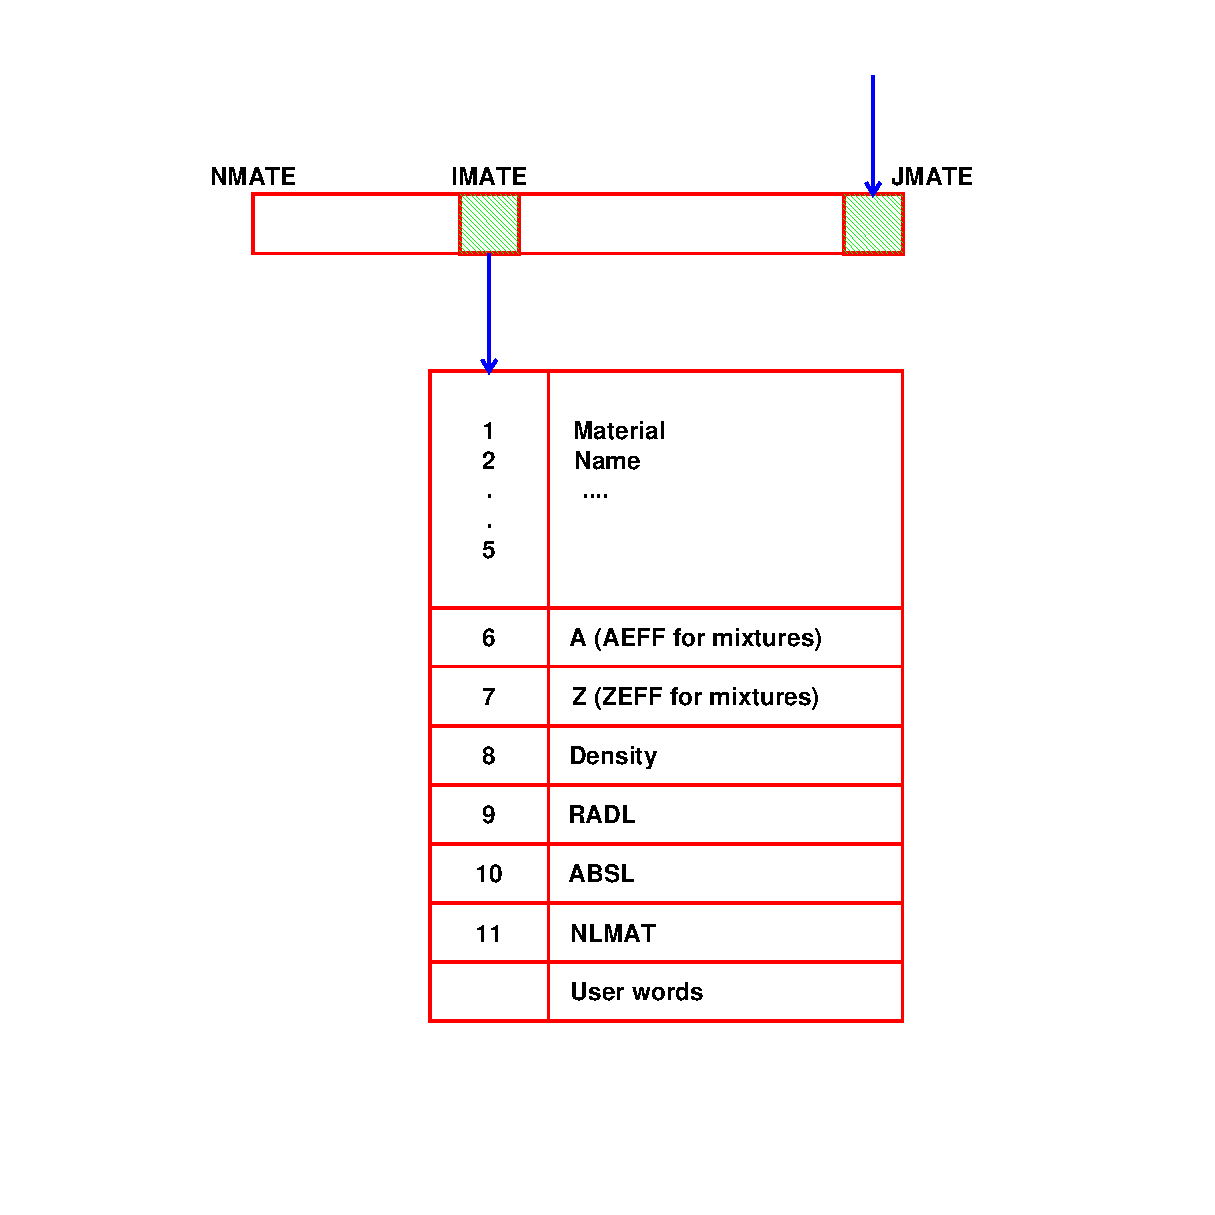
\epsfig{file=eps/cons199-1.eps,width=\linewidth}
      \caption{{\tt JMA = LQ(JMATE-IMATE)} pointer to material {\tt IMATE}}
      \label{cons199-1}
\end{figure}

When the subroutine GPHYSI is called at initialisation time the
following substructure is created for each material whose number
is refered to by any of the user defined tracking media.

\begin{figure}[p]
      \centering
      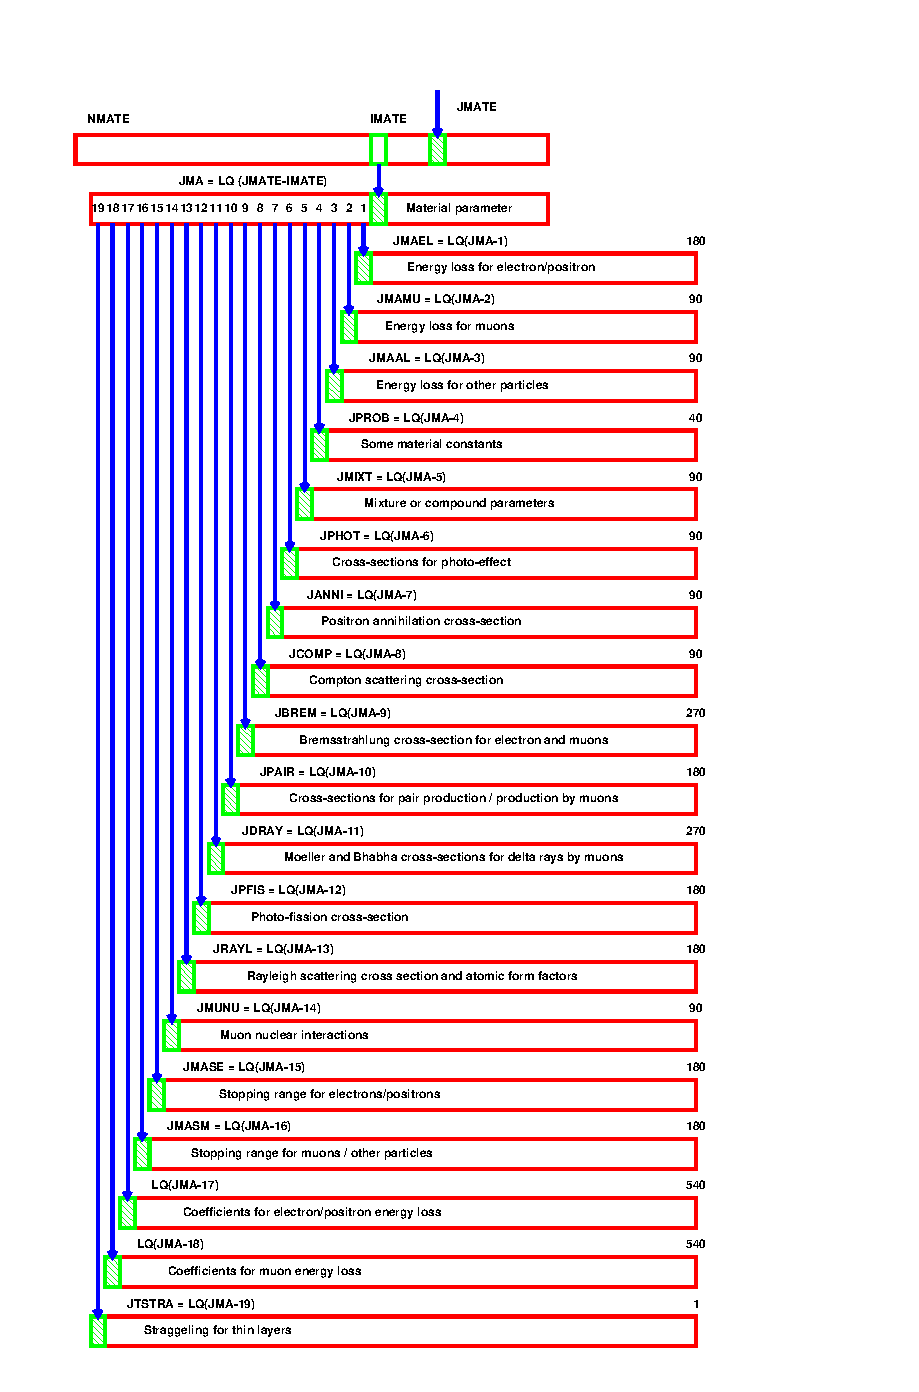
\epsfig{file=eps/cons199-2.eps,height=.95\textheight}
      \caption{Material data structure}
      \label{cons199-2}
\end{figure}

{\bf Note:}
The energy losses are stored in ${\rm GeV \: cm^{-1}}$. The inverse of
the macroscopic cross-section (i.e. the mean free path, in cm), is stored
instead of the cross-section, to speed up the calculation of the distance
to the next interaction point.
 
\section{Energy binning}
 
\begin{center}
\begin{tabular}{|c|l|l|}
\hline
IDECAD  &Bin number  &Energy range \\
& &IEKBIN    \\
\hline
 
1  &1 $\rightarrow$ 10  &10 KeV $\rightarrow$ 79.43 KeV          \\
2  &11 $\rightarrow$ 20  &100 KeV $\rightarrow$ 794.3 KeV       \\
3  &21 $\rightarrow$ 30  &1 MeV $\rightarrow$ 7.943 MeV           \\
4  &31 $\rightarrow$ 40  &10 MeV $\rightarrow$ 79.43 MeV         \\
5  &41 $\rightarrow$ 50  &100 MeV $\rightarrow$ 794.3 MeV       \\
6  &51 $\rightarrow$ 60  &1 GeV $\rightarrow$ 7.943 GeV           \\
7  &61 $\rightarrow$ 70  &10 GeV $\rightarrow$ 79.43 GeV         \\
8  &71 $\rightarrow$ 80  &100 GeV $\rightarrow$ 794.3 GeV       \\
9  &81 $\rightarrow$ 90  &1 TeV $\rightarrow$ 7.943 TeV           \\
\hline
\end{tabular}
\end{center}
 
The values of the bins are kept in the array ELOW(90) in /GCMULO/ :
 
\[
 \mbox{ELOW}(i) = 10 ^ { \frac{i-1}{10} - 5 } [ \mbox{GeV} ]
\]
 
\section{Energy loss for electrons and positrons}
 
Words 1 to 90, for electrons:  DE/DX = Ionisation (Moller) +brems.
 
Words 91 to 180, for positrons:  DE/DX = Ionisation (Bhabha) +brems.
[PHYS 330, 340].
 
\section{Energy loss for muons}
 
  DE/DX = Ionisation +brems. +Direct \Pep\Pem production +Nuclear interacti     on
[PHYS 430, 440, 450].
 
\section{Energy loss for other charged particles}
 
  DE/DX = Ionisation
 
The values are computed for a proton (mass Mp). For any other
particle with mass M and kinetic energy T,
one has to compute the equivalent proton kinetic energy as T*Mp/M
and look at the corresponding energy binning [PHYS 430].
 
\section{Some material constants}
 
Various constants which are material dependent and needed to compute the
cross-sections.
 
See routine GPROBI.
 
\section{Mixture and compound parameters}
 
Words 1 to 4*NLM  where  NLM is the number of mixture or compound
components [CONS110].
 
\section{Photo-electric effect. Muon nuclear interaction}
 
As the photo-electric effect vanishes at high energies
whereas the muon nuclear
interaction cross-section is null at low energies, the two effects are
stored within the same bank in order to save space.
 
From 10 KeV to 50 MeV : Photo-electric effect mean free path [PHYS 230]
From 1 GeV to 10 TeV : Muon nuclear interaction mean free path
[PHYS 460].
 
\section{Positron annihilation}
 
[PHYS 350].
 
\section{Compton scattering}
 
[PHYS 220].
 
\section{Bremsstrahlung for electrons and muons}
 
Words 1 to 90, mean free path for electrons [PHYS 340]
Words 91 to 180, mean free path for muons [PHYS 440].
 
\section{Pair production by gammas and muons}
 
Words 1 to 90, for gammas [PHYS 210].
Words 91 to 180, for muons [PHYS 450].
 
\section{Delta ray production by electrons and muons}
 
Words 1 to 90, for \Pem\Pem $\rightarrow$ \Pem\Pem [PHYS 330].
 
Words 91 to 180, for \Pep\Pem $\rightarrow$ \Pep\Pem [PHYS 330]
 
Words 181 to 270, for \Pem $\rightarrow$ \Pem [PHYS 430].
 
\section{Photo-fission}
 
Only for material with atomic number A>200 [PHYS 240].
%\end{document}
 
 

%%%%%%%%%%%%%%%%%%%%%%%%%%%%%%%%%%%%%%%%%%%%%%%%%%%%%%%%%%%%%%%%%%%
%                                                                 %
%  GEANT manual in LaTeX form                                     %
%                                                                 %
%  Version 1.00                                                   %
%                                                                 %
%  Last Mod. 12 June 1993 1700   MG                               %
%                                                                 %
%%%%%%%%%%%%%%%%%%%%%%%%%%%%%%%%%%%%%%%%%%%%%%%%%%%%%%%%%%%%%%%%%%%
\Origin{R.Brun}            
\Revision{F.Carminati, M.Maire}
\Version{Geant 3.16}           \Routid{CONS200}
\Submitted{01.06.83}           \Revised{08.12.93}
\Makehead{Tracking medium parameters}
\section*{Description of the routines}
\Shubr{GSTMED}{(ITMED,NATMED,NMAT,ISVOL,IFIELD,FIELDM,TMAXFD,STEMAX,
                DEEMAX,EPSIL,STMIN,UBUF,NWBUF)}
This routine associates a set of tracking parameters to a material, defining
a so-called {\it tracking medium}. Every {\tt GEANT} volume must be 
associated to an existing tracking medium. The routine
stores the parameters of the tracking
medium {\tt ITMED} in the data structure {\tt JTMED}.
\begin{DLtt}{MMMMMMMM}
\item[ITMED]      ({\tt INTEGER}) tracking medium number;
\item[NATMED]     ({\tt CHARACTER*20}) tracking medium name;
\item[NMAT]       ({\tt INTEGER}) material number corresponding to {\tt ITMED};
\item[ISVOL]      ({\tt INTEGER}) {\it sensitivity} flag (see later):
\begin{DLtt}{MMMM}
\item[$\leq$0] not a sensitive volume;
\item[$>$0] sensitive volume;
\end{DLtt}
\item[IFIELD]     ({\tt INTEGER}) magnetic field flag:
\begin{DLtt}{MMMM}
\item[=0]         no magnetic field;
\item[=1]         strongly 
inhomogeneous magnetic field (returned by the user function
\Rind{GUFLD}): tracking performed with the Runge-Kutta method by the
routine \Rind{GRKUTA};
\item[=2]         inhomogeneous magnetic field (returned by the user function
\Rind{GUFLD}), tracking along a helix performed by the routine \Rind{GHELIX};
\item[=3]         uniform magnetic field along the {\tt z} axis of strength
{\tt FIELDM}, tracking performed along a helix by the routine \Rind{GHELX3};
\end{DLtt}
\item[FIELDM]     ({\tt REAL}) maximum field value (in Kilogauss);
\item[TMAXFD]     ({\tt REAL}) maximum angular deviation due to the magnetic
field permitted in one step (in degrees);
\item[STEMAX]     ({\tt REAL}) maximum step permitted (cm);
\item[DEEMAX]     ({\tt REAL}) maximum fractional energy loss in one step ($0<$
                  {\tt DEEMAX} $\leq 1$);
\item[EPSIL]      ({\tt REAL}) boundary crossing precision (cm);
\item[STMIN]      ({\tt REAL}) minimum value for the maximum step imposed by 
energy loss, multiple scattering, \v{C}erenkov or magnetic field effects (cm);
\item[UBUF]       ({\tt REAL}) array of {\tt NWBUF} additional user parameters;
\item[NWBUF]      ({\tt INTEGER}) number of additional user parameters.
\end{DLtt}
 
{\bf Note:} the tracking medium number can in principle be any positive
integer from 1 to 65,535. However this number is used directly by {\tt GEANT}
as the number of the pointer to the data structure where the information
is stored. When a pointer is defined,
all pointers from 1 to the one allocated are created, if not already existing.
Every time data structures are moved in memory, all the
links are potentially scanned for update. This can be time consuming and
it can seriously affect performances. So a continuous
range of numbers should be used for tracking media.

\Shubr{GFTMED}{(ITMED,NATMED*,NMAT*,ISVOL*,IFIELD*,FIELDM*,TMAXFD*,
                STEMAX*,DEEMAX*,EPSIL*,STMIN*,UBUF*,NWBUF*)}
 
Extracts the parameters of the tracking medium {\tt ITMED}
from the data structure {\tt JTMED}.
 
\Shubr{GPTMED}{(ITMED)}
 
Prints the tracking medium parameters for the given medium.
\begin{DLtt}{MMMMM}
\item[ITMED]      ({\tt INTEGER}) tracking medium to be printed,
all tracking media if {\tt ITMED}=0.
\end{DLtt}

\section*{Automatic calculation of the tracking parameters}

The results of the simulation depend critically on the choice of the tracking
medium parameters. To make of {\tt GEANT} a reliable and consistent predictive
tool, the calculation of these parameters has been automated.
In a normal GEANT run, the variable {\tt IGAUTO} in common
\FCind{/GCTRAK/} is set to 1. In this case the following parameters 
are calculated by the program:
\begin{eqnarray*}
\mbox{\tt TMAXFD} & = & \left\{
\begin{array}{LL}
20^{\circ} & \mbox{if {\tt TMAXFD} $\leq 0$ or {\tt TMAXFD} $ > 20$} \\
\mbox{\it input value} & \mbox{if $0 <$ {\tt TMAXFD} $\leq 20$}
\end{array} \right . \\
\mbox{\tt STEMAX} & = & \phantom{\{} 
\begin{array}{LL} \mbox{\tt BIG} (=10^{10}) \end{array} \\
\mbox{\tt DEEMAX} & = & \left \{
\begin{array}{LL}
0.25 & \parbox[t]{10cm}{if {\tt ISVOL} $= 0$ and $X_{0} \leq 2cm$, 
where $X_{0}$ is the radiation length of the material} \\
0.25-\frac{0.2}{\sqrt{X_{0}}} & \mbox{otherwise}
\end{array} \right . \\
\mbox{\tt STMIN} & = & \left\{
\begin{array}{LL}
\frac{2 R}{\sqrt{X_{0}}} & \mbox{if {\tt ISVOL} $=0$} \\ [.2cm]
\frac{5 R}{\sqrt{X_{0}}} & \mbox{if {\tt ISVOL} $\neq 0$}
\end{array} \right . 
\end{eqnarray*}

where $R$ is the range in cm of an electron of energy {\tt CUTELE}+200keV.

If the {\tt IGAUTO} variable is set to 0 via the {\tt AUTO} data record, 
then value given by the user for the above parameters is accepted as the
true parameter value if $>0$, while automatic calculation still takes place
in case the input value is negative.

Users are strongly recommended to begin their simulation with the parameters
as calculated by {\tt GEANT}. Users who want to modify any of the above
parameters must be sure they understand their function in the program and
the implications of a change.

The {\tt EPSIL} parameter represents the absolute precision with which the
tracking is performed. It has a double meaning. When tracking in magnetic
field, {\tt EPSIL} is the minimum distance for which boundaries are
checked. A particle nearer than {\tt EPSIL} to the boundary is considered
as exiting the current volume. If the end point of the step of a particle in
magnetic field is distant less than {\tt EPSIL} along each axis 
from what would be the end point in absence of magnetic field, then no boundary 
checking is performed. 

In all cases, when a particle is going to reach the
boundary of the current volume with the current step, the step length is 
increased by a quantity ({\tt PREC}, common \FCind{/GCTMED/}) which is set to the 
minimum between $0.1 \times {\tt EPSIL}$
and 10 micron at the beginning of the tracking. This quantity is recalculated
at every step according to the formula:
\begin{equation}
\mbox{\tt PREC} 
=\max \left [ \min \left(\frac{\mbox{\tt EPSIL}}{10}, 10 \mu \right ) ,
\max \left [ | x |, | y |, | z |, S \right ) \times \epsilon \right ]
\end{equation}
Where $x, y, z$ are the current coordinates of the particle, $S$ is the length
of the track, and $\epsilon$ is the assumed machine precision.
$\epsilon$ (called {\tt EPSMAC} in the program) is initially set to
$10^{-6}$ for 32 bits machines and $10^{-11}$ for 64 bits machines.
During the tracking, every fifth time that a particle tries unsuccessfully
to exit from the same volume, the machine precision is multiplied by the
number of trials. This accounts for additional losses of precision due to
transformation of coordinates and region of the floating point range where
the real machine precision is different from the above (this happens 
in particular on IBM mainframes with 370 floating point number representation).

%%%%%%%%%%%%%%%%%%%%%%%%%%%%%%%%%%%%%%%%%%%%%%%%%%%%%%%%%%%%%%%%%%%
%                                                                 %
%  GEANT manual in LaTeX form                                     %
%                                                                 %
%  Michel Goossens (for translation into LaTeX)                   %
%  Version 1.00                                                   %
%  Last Mod. Jan 24 1991  1300   MG + IB                          %
%                                                                 %
%%%%%%%%%%%%%%%%%%%%%%%%%%%%%%%%%%%%%%%%%%%%%%%%%%%%%%%%%%%%%%%%%%%
\Origin{R.Brun,F.Bruyant}
\Documentation{same}
\Version{Geant 3.16}\Routid{CONS210}
\Submitted{11.02.86}     \Revised{08.12.93}
\Makehead{Special Tracking  Parameters}
 
\Shubr{GSTPAR}{(ITMED,CHPAR,PARVAL)}
 
\begin{DLtt}{MMMMMMMMMM}
\item[ITMED]   ({\tt INTEGER}) tracking medium number;
\item[CHPAR]   ({\tt CHARACTER*4}) character string, name of the variable 
to be modified;
\item[PARVAL]  ({\tt REAL}) new value (must be given as a floating point).
\end{DLtt}
\begin{center} 
\begin{tabular}{|>{\ttfamily}r@{}>{\ttfamily}r@{\quad=\quad}>{\ttfamily}l|>{\ttfamily}l|l|}
 \hline
\multicolumn{3}{|c|}{Default parameters}
& \multicolumn{1}{c|}{Parameter name} 
& \multicolumn{1}{c|}{Default value} \\
\hline
Q(JTMN & +1) & CUTGAM & CUTGAM & 0.001GeV \\
Q(JTMN & +2) & CUTELE & CUTELE & 0.001GeV \\
Q(JTMN & +3) & CUTNEU & CUTNEU & 0.01GeV  \\
Q(JTMN & +4) & CUTHAD & CUTHAD & 0.01GeV  \\
Q(JTMN & +5) & CUTMUO & CUTMUO & 0.01GeV  \\
Q(JTMN & +6) & BCUTE  & BCUTE  & \texttt{CUTGAM}   \\
Q(JTMN & +7) & BCUTM  & BCUTM  & \texttt{CUTGAM}   \\
Q(JTMN & +8) & DCUTE  & DCUTE  & 10.TeV   \\
Q(JTMN & +9) & DCUTM  & DCUTM  & 10.TeV   \\
Q(JTMN & +10)& PPCUTM & PPCUTM & 0.01GeV  \\
Q(JTMN & +11)& IPAIR  &  PAIR  & 1        \\
Q(JTMN & +12)& ICOMP  &  COMP  & 1        \\
Q(JTMN & +13)& IPHOT  &  PHOT  & 1        \\
Q(JTMN & +14)& IPFIS  &  PFIS  & 0        \\
Q(JTMN & +15)& IDRAY  &  DRAY  & 2        \\
Q(JTMN & +16)& IANNI  &  ANNI  & 1        \\
Q(JTMN & +17)& IBREM  &  BREM  & 1        \\
Q(JTMN & +18)& IHADR  &  HADR  & 1        \\
Q(JTMN & +19)& IMUNU  &  MUNU  & 0        \\
Q(JTMN & +20)& IDCAY  &  DCAY  & 1        \\
Q(JTMN & +21)& ILOSS  &  LOSS  & 2        \\
Q(JTMN & +22)& IMULS  &  MULS  & 1        \\
Q(JTMN & +26)& GHEISHA   & GHCOR1 & see \texttt{[PHYS700]}  \\
Q(JTMN & +27)& MODEL     & BIRK1  & see \texttt{[PHYS337]}  \\
Q(JTMN & +28)& RKB     & BIRK2  & see \texttt{[PHYS337]}  \\
Q(JTMN & +29)& C     & BIRK3  & see \texttt{[PHYS337]}  \\
Q(JTMN & +31)& ILABS  & LABS  & see \texttt{[PHYS260]}  \\
Q(JTMN & +32)& ISYNC  & SYNC  & see \texttt{[PHYS360]}  \\
Q(JTMN & +33)& ISTRA  & STRA  & see \texttt{[PHYS333]} \\
\hline
\end{tabular}
\end{center} 
 
The data structure \texttt{JTMED} contains the standard tracking parameters
(\texttt{CUTS} and flags to control the physics processes) which are used by
default for all tracking media. It is possible to redefine individually
with \Rind{GSTPAR} any of these parameters for a given tracking medium.
For example to change \texttt{CUTGAM} to 0.0001 for tracking medium \texttt{ITMED}:
\begin{center}
 \texttt{CALL GSTPAR(ITMED,'CUTGAM',0.0001)}
\end{center}

For more information on default values for \texttt{IDRAY} and \texttt{ILOSS} see
\texttt{[BASE040]}.
 
The default tracking medium parameters are stored in the bank whose
pointer is stored in the \texttt{JTMED} variable. In this case in the
above table \texttt{JTMN} = \texttt{JTMED}. In the case one or more of
the above parameters has been modified for a specific tracking
medium, the whole parameter set is stored in the next bank of the
given trackin medium. In this case \texttt{JTMN} = \texttt{LQ(JTM)} in
the above table, where \texttt{JTM} is the pointer to the bank of the
tracking medium, i.e. \texttt{JTM} = \texttt{LQ(JTMED-ITMED)}.
 
{\bf Note}
 
At tracking time the parameters above are copied
from \texttt{JTMN} into the common blocks
\FCind{/GCCUTS/} and \FCind{/GCPHYS/}. \Rind{GSTPAR} must be called before
\Rind{GPHYSI}.
%\end{document}
 

%%%%%%%%%%%%%%%%%%%%%%%%%%%%%%%%%%%%%%%%%%%%%%%%%%%%%%%%%%%%%%%%%%%
%                                                                 %
%  GEANT manual in LaTeX form                                     %
%                                                                 %
%  Michel Goossens (for translation into LaTeX)                   %
%  Version 1.00                                                   %
%  Last Mod. Jan 24 1991  1300   MG + IB                          %
%                                                                 %
%%%%%%%%%%%%%%%%%%%%%%%%%%%%%%%%%%%%%%%%%%%%%%%%%%%%%%%%%%%%%%%%%%%
\Origin{R.Brun, G.N.Patrick}
\Version{Geant 3.15}\Routid{CONS300}
\Submitted{01.06.83}               \Revised{13.05.92}
\Makehead{Particle definition}
 
\Shubr{GPART}{}
 
Stores the standard particle constants in the data structure
{\tt JPART} and, through the routine \Rind{GSDK}, their decay modes 
{\tt [CONS310]}.
 
\begin{center}
\begin{tabular}{|l|r|l|r|r@{}l|}
\hline
\makebox[2.5cm][l]{Particle} & No.  & 
\makebox[3.2cm][l]{Mass(GeV)} &   Charge & 
\makebox[2.3cm][l]{Life time(sec)} & 
\makebox[1.3cm]{}  \\
\hline
Gamma        & 1 &0.0           &  0 & stable & \hspace{.2cm} ($10^{15}$) \\
Positron     & 2 &0.00051099906 &  1 &  stable &          \\
Electron     & 3 &0.00051099906 & -1 &  stable &          \\
Neutrino     & 4 & 0.0          &  0 &  stable &          \\
Muon +       & 5 &0.105658389   &  1 & $2.19703 $ & $\: \times 10^{-6}$\\
Muon -       & 6 &0.105658389   & -1 & $2.19703 $ & $\: \times 10^{-6}$  \\
Pion 0       & 7 &0.1349764     &  0 & $8.4 $ & $\: \times 10^{-17}$     \\
Pion +       & 8 &0.1395700     &  1 & $2.603 $ & $\: \times 10^{-8}$   \\
Pion -       & 9 &0.1395700     & -1 & $2.603 $ & $\: \times 10^{-8} $  \\
Kaon 0 long  &10 &0.497672      &  0 & $5.17 $ & $\: \times  10^{-8}$    \\
Kaon +       &11 &0.493677      &  1 & $1.237 $ & $\: \times 10^{-8}$   \\
Kaon -       &12 &0.493677      & -1 & $1.237 $ & $\: \times 10^{-8}$    \\
Neutron      &13 &0.93956563    &  0 & $  887.0 $ &                 \\
Proton       &14 &0.93827231    &  1 & stable    &         \\
Antiproton   &15 &0.93827231    & -1 & stable    &         \\
Kaon 0 short &16 &0.497672      &  0 & $ 8.926 $ & $\: \times 10^{-11}$   \\
Eta          &17 &0.54745       &  0 & $ 5.485   $ & $\: \times 10^{-19}$ \\
Lambda       &18 &1.115684      &  0  & $ 2.632 $ & $\: \times 10^{-10}$    \\
Sigma +      &19 &1.18937       &  1  & $ 7.99   $ & $\: \times 10^{-11}$     \\
Sigma 0      &20 &1.19255       &  0  & $ 7.40 $ & $\: \times  10^{-20}$   \\
Sigma -      &21 &1.197436      & -1  & $1.479 $ & $\: \times  10^{-10}$   \\
Xi 0         &22 &1.3149        &  0  & $2.90 $ & $\: \times  10^{-10}$   \\
Xi -         &23 &1.32132       & -1  & $1.639 $ & $\: \times 10^{-10}$   \\
Omega        &24 &1.67245       & -1  & $ 8.22 $ & $\: \times 10^{-11}$   \\
Antineutron  &25 &0.93956563    &  0  & $ 887.0 $  &           \\
Antilambda   &26 &1.115684      &  0  &  $ 2.632 $ & $\: \times 10^{-10}$  \\
Antisigma -  &27 &1.18937       & -1  &  $ 7.99 $ & $\: \times 10^{-11}$   \\
Antisigma 0  &28 &1.19255       &  0  &  $ 7.40 $ & $\: \times  10^{-20}$   \\
Antisigma +  &29 &1.197436      &  1  &  $ 1.479 $ & $\: \times 10^{-10}$   \\
Antixi 0     &30 &1.3149        &  0  &  $ 2.90 $ & $\: \times   10^{-10}$   \\
Antixi +     &31 &1.32132       &  1  &  $ 1.639 $ & $\: \times 10^{-10}$  \\
\hline
\end{tabular}
\end{center}
\newpage
\begin{center}
\begin{tabular}{|l|r|l|r|r@{}l|}
\hline
\makebox[2.5cm][l]{Particle} & No.  & 
\makebox[3.2cm][l]{Mass(GeV)} &   Charge & 
\makebox[2.3cm][l]{Life time(sec)} & 
\makebox[1.3cm]{}  \\
\hline
Antiomega +  &32    &1.67245    &   1     &  $ 8.22 $ & $\: \times  10^{-11}$  \\
%Tau +      &33    &1.7841     &   1     &  $ 3.04 $ & $\: \times 10^{-13}$   \\
%Tau -      &34    &1.7841     &   1     &  $ 3.04 $ & $\: \times 10^{-13}$  \\
%D+         &35    &1.8693     &   1     &  $ 1.062 $ & $\: \times 10^{-12}$  \\
%D-         &36    & 1.8693    &  -1     &  $ 1.062 $ & $\: \times 10^{-12}$  \\
%D0         &37    & 1.8645    &   0     &  $ 4.28 $ & $\: \times 10^{-13}$  \\
%Anti D0    &38    & 1.8645    &   0     &  $4.28 $ & $\: \times  10^{-13}$   \\
%DS+        &39    & 1.9693    &   1     &  $ 4.36 $ & $\: \times 10^{-13}$   \\
%DS-        &40    & 1.9693    &  -1     &  $ 4.36 $ & $\: \times 10^{-13}$   \\
%Lambda C+  &41    & 2.2849    &   1     &  $ 1.79 $ & $\: \times 10^{-13}$    \\
%W+         &42    & 81.   &   1     &  $ 9.4  $ & $\: \times  10^{-26}$    \\
%W-         &43    & 81.   &  -1     &  $ 9.4  $ & $\: \times  10^{-26}$    \\
%Z0         &44    & 92.4   &   0     &  $ 7.74 $ & $\: \times  10^{-26}$   \\
Deuteron     &45    &1.875613   &   1     &  stable  &           \\
Tritium      &46    &2.80925  &   1     &  stable  &            \\
Alpha        &47    &3.727417   &   2     &   stable &          \\
Geantino     &48    & 0        &   0     &  stable   &       \\
He3          &49    &2.80923    &   2     &   stable     &      \\
Cerenkov     &50    &0          &   0     &   stable     &      \\
\hline
\end{tabular}
\end{center}
 
\Shubr{GPIONS}{}
 
Stores the standard ions constants in the data structure
{\tt JPART}.
 
\begin{center}
\begin{tabular}{|l|r|l|r|r@{}l|}
\hline
\makebox[2.5cm][l]{Particle} & No.  & 
\makebox[3.2cm][l]{Mass(GeV)} &   Charge & 
\makebox[2.3cm][l]{Life time(sec)} & 
\makebox[1.3cm]{}  \\
\hline
Li6   &  61 &     5.60305  &   3  &  1000 & \\
Li7   &  62 &     6.53536  &   3  &  1000 & \\
Be7   &  63 &     6.53622  &   4  &  1000 & \\
Be9   &  64 &     8.39479  &   4  &  1000 & \\
B10   &  65 &     9.32699  &   5  &  1000 & \\
B11   &  66 &    10.25510  &   5  &  1000 & \\
C12   &  67 &    11.17793  &   6  &  1000 & \\
N14   &  68 &    13.04378  &   7  &  1000 & \\
O16   &  69 &    14.89917  &   8  &  1000 & \\
F19   &  70 &    17.69690  &   9  &  1000 & \\
Ne20  &  71 &    18.62284  &  10  &  1000 & \\
Na23  &  72 &    21.41483  &  11  &  1000 & \\
Mg24  &  73 &    22.34193  &  12  &  1000 & \\
Al27  &  74 &    25.13314  &  13  &  1000 & \\
Si28  &  75 &    26.06034  &  14  &  1000 & \\
P31   &  76 &    28.85188  &  15  &  1000 & \\
S32   &  77 &    29.78180  &  16  &  1000 & \\
Cl35  &  78 &    32.57328  &  17  &  1000 & \\
Ar36  &  79 &    33.50356  &  18  &  1000 & \\
K39   &  80 &    36.29447  &  19  &  1000 & \\
Ca40  &  81 &    37.22492  &  20  &  1000 & \\
Sc45  &  82 &    41.87617  &  21  &  1000 & \\
Ti48  &  83 &    44.66324  &  22  &  1000 & \\
V51   &  84 &    47.45401  &  23  &  1000 & \\
Cr52  &  85 &    48.38228  &  24  &  1000 & \\
Mn55  &  86 &    51.17447  &  25  &  1000 & \\
Fe56  &  87 &    52.10307  &  26  &  1000 & \\
Co59  &  88 &    54.89593  &  27  &  1000 & \\
Ni58  &  89 &    53.96644  &  28  &  1000 & \\
Cu63  &  90 &    58.61856  &  29  &  1000 & \\
Zn64  &  91 &    59.54963  &  30  &  1000 & \\
\hline
\end{tabular}
\end{center}
\newpage
\begin{center}
\begin{tabular}{|l|r|l|r|r@{}l|}
\hline
\makebox[2.5cm][l]{Particle} & No.  & 
\makebox[3.2cm][l]{Mass(GeV)} &   Charge & 
\makebox[2.3cm][l]{Life time(sec)} & 
\makebox[1.3cm]{}  \\
\hline
Ge74  &  92 &    68.85715  &  32  &  1000 & \\
Se80  &  93 &    74.44178  &  34  &  1000 & \\
Kr84  &  94 &    78.16309  &  36  &  1000 & \\
Sr88  &  95 &    81.88358  &  38  &  1000 & \\
Zr90  &  96 &    83.74571  &  40  &  1000 & \\
Mo98  &  97 &    91.19832  &  42  &  1000 & \\
Pd106 &  98 &    98.64997  &  46  &  1000 & \\
Cd114 &  99 &   106.10997  &  48  &  1000 & \\
Sn120 & 100 &   111.68821  &  50  &  1000 & \\
Xe132 & 101 &   122.86796  &  54  &  1000 & \\
Ba138 & 102 &   128.45793  &  56  &  1000 & \\
Ce140 & 103 &   130.32111  &  58  &  1000 & \\
Sm152 & 104 &   141.51236  &  62  &  1000 & \\
Dy164 & 105 &   152.69909  &  66  &  1000 & \\
Yb174 & 106 &   162.02245  &  70  &  1000 & \\
W184  & 107 &   171.34924  &  74  &  1000 & \\
Pt194 & 108 &   180.67513  &  78  &  1000 & \\
Au197 & 109 &   183.47324  &  79  &  1000 & \\
Hg202 & 110 &   188.13451  &  80  &  1000 & \\
Pb208 & 111 &   193.72907  &  82  &  1000 & \\
U238  & 112 &   221.74295  &  92  &  1000 & \\
\hline
\end{tabular}
\end{center}
 
{\bf Note}
 
It is possible for the user to define more particles or to redefine
some characteristics of the particles currently defined in {\tt GEANT},
but this must be done with extreme care. In particular, the mass and
charge of most particles are stored independently in {\tt FLUKA}, and
any change made via \Rind{GSPART} will not affect these values. Removing
particles from the list can lead to unpredictable results and it is
strongly discouraged.
 
The user who needs 
more particles, or wants to partly override the standard values,
can do that via the routines \Rind{GSPART} and \Rind{GSDK}.
 
All data taken from M. Aguilar Benitez \cite{bib-AGUI} and updated with
the values of the PDG \cite{bib-PDGD}.
 
\Shubr{GSPART}{(IPART,CHNPAR,ITRTYP,AMASS,CHARGE,TLIFE,UB,NWB)}
 
Stores the constants describing the particle.
{\tt IPART} in the data structure {\tt JPART}.
\begin{DLtt}{MMMMMMMM}
\item[IPART]   ({\tt INTEGER}) particle number;
\item[CHNPAR]  ({\tt CHARACTER*20)} particle name;
\item[ITRTYP]  ({\tt INTEGER}) type of tracking routine requested:
\begin{DLtt}{MMMM}
\item[1] particle tracked by \Rind{GTGAMA};
\item[2] particle tracked by \Rind{GTELEC};
\item[3] particle tracked by \Rind{GTNEUT};
\item[4] particle tracked by \Rind{GTHADR};
\item[5] particle tracked by \Rind{GTMUON};
\item[6] geantino tracked by \Rind{GTNINO};
\item[7] heavy ion tracked by \Rind{GTCKOV};
\item[8] light photon tracked by \Rind{GTHION};
\end{DLtt}
\item [AMASS]  ({\tt REAL}) particle mass in GeV;
\item[CHARGE]  ({\tt REAL}) particle charge;
\item[TLIFE]   ({\tt REAL}) particle life time (in seconds);
\item[UB]      ({\tt REAL}) array of {\tt NWB} user additional parameters;
\item[NWB]     ({\tt INTEGER}).
\end{DLtt}
 
\Shubr{GFPART}{(IPART,CHNPAR*,ITRTYP*,AMASS*,CHARGE*,TLIFE*,UB*,NWB*)}
 
Extracts the constants describing the
particle {\tt IPART} from the data structure {\tt JPART}.
 
\Shubr{GPPART}{(IPART)}
 
Prints the particle constants
for  particle {\tt IPART} (for all particles if {\tt IPART=0}).

%%%%%%%%%%%%%%%%%%%%%%%%%%%%%%%%%%%%%%%%%%%%%%%%%%%%%%%%%%%%%%%%%%%
%                                                                 %
%  GEANT manual in LaTeX form                                     %
%                                                                 %
%  Michel Goossens (for translation into LaTeX)                   %
%  Version 1.00                                                   %
%  Last Mod. Jan 24 1991  1300   MG + IB                          %
%                                                                 %
%%%%%%%%%%%%%%%%%%%%%%%%%%%%%%%%%%%%%%%%%%%%%%%%%%%%%%%%%%%%%%%%%%%
\Origin{R.Brun, G.N.Patrick}
\Version{Geant 3.16}\Routid{CONS310}
\Submitted{23.01.84}     \Revised{19.10.94}
\Makehead {Branching Ratios and Particle Decay Modes}
\Shubr{GSDK}{(IPART,BRATIO,MODE)}
\begin{DLtt}{MMMMMMMM}
\item[IPART]       ({\tt INTEGER}) {\tt GEANT} particle number;
\item[BRATIO]   ({\tt REAL}) array of branching ratios in \%,
maximum 6;
\item[MODE]     ({\tt INTEGER}) array of partial decay modes.
\end{DLtt}
\Rind{GSDK} stores the branching ratios and partial decay modes for two
and three body particle decays into the data structure {\tt JPART}.
The decay modes should be coded into the array {\tt MODE} such that:
\begin{center}
{\tt MODE(I) =  10$^4$ N3 + 10$^2$ N2 + N1} \hspace{2cm}
for {\tt I=1,$\cdots$,6}
\end{center}
where:
\begin{DLtt}{MMMM}
\item [N1]     particle number for decay product 1;
\item [N2]     particle number for decay product 2;
\item [N3]     particle number for decay product 3 (if any).
\end{DLtt}
It is important to note the following:
\begin{itemize}
\item  prior to calling \Rind{GSDK}, all parent and secondary particles should
have been defined by \Rind{GSPART};
\item  if less than six decay modes are defined the remaining elements
of {\tt BRATIO} and {\tt MODE} must be set to zero.
\end{itemize}
For a given particle, {\tt IPART}, the decay parameters are stored into
the {\tt JPART} data structure as follows:

\begin{DLtt}{MMMMMMMMMM}
\item[JPA] {\tt = LQ(JPART-IPART)} pointer to the bank containing the
information on the particle {\tt IPART};
\item[JDK1] {\tt = LQ(JPA-1)} pointer to branching ratios bank;
 \item[JDK2] {\tt = LQ(JPA-2)} pointer to decay modes bank;
\item[BR(I)] {\tt = Q(JDK1+I)}     I$^{th}$ branching ratio;
 \item[MODE(I)] {\tt = IQ(JDK2+I)}   I$^{th}$ decay mode, where
{\tt I=1,$\cdots$,6}.
\end{DLtt}
When a particle decays during tracking,
the routine \Rind{GDECAY} is called. If branching ratios and modes
have been stored by \Rind{GSDK}, then \Rind{GDECAY}
generates the decay products in the 2- or 3-body phase space.
If no branching ratios have been defined by \Rind{GSDK},
the user routine
\Rind{GUDCAY} is called, where the user can code special decay modes and
branching ratios. All data taken from Aguilar Benitez \cite{bib-AGUI}.
\newpage

\[
\begin{array}{|l|l|}
\hline
\makebox[4cm][|l|]{Parent particle} &
\makebox[8cm][c|]{Decay \hfill Branching ratio (\%)} \\ \hline

\mu^{\pm}      &
\begin{array}{lr}
\makebox[5cm][l]{$e^{\pm}\nu\nu$}        &  100.00
\end{array} \\ \hline

\pi^{0}        &
\begin{array}{lr}
\makebox[5cm][l]{$\gamma\gamma$}         &  98.802   \\
\gamma e^+e^-          &  1.198
\end{array} \\ \hline

\pi^{\pm}      &
\begin{array}{lr}
\makebox[5cm][l]{$\mu^{\pm}\nu$}         &  100.00 \\
\end{array} \\ \hline

K^0_{l}        &
\begin{array}{lr}
\makebox[5cm][l]{$\pi^- e^+ \nu$}        &  19.35    \\
\pi^+ e^- \nu          &  19.35    \\
\pi^-\mu^+\nu          &  13.50    \\
\pi^+\mu^-\nu          &  15.50    \\
\pi^0\pi^0\pi^0        &  21.50    \\
\pi^+\pi^-\pi^0        &  12.38
\end{array} \\ \hline

K^{\pm}        &
\begin{array}{lr}
\makebox[5cm][l]{$\mu^{\pm}\nu$}         & 63.51     \\
\pi^{\pm}\pi^0         & 21.17     \\
\pi^{\pm}\pi^+\pi^-    &  5.59     \\
e^{\pm}\nu\pi^0        &  4.82     \\
\mu^{\pm}\nu\pi^0      &  3.18     \\
\pi^{\pm}\pi^0\pi^0    &  1.73
\end{array} \\ \hline

K^0_s          &
\begin{array}{lr}
\makebox[5cm][l]{$\pi^+\pi^-$}           &  68.61    \\
\pi^0\pi^0             &  31.39
\end{array} \\ \hline

\eta           &
\begin{array}{lr}
\makebox[5cm][l]{$\gamma\gamma$}         &  38.80    \\
\pi^0\pi^0\pi^0        &  31.90    \\
\pi^+\pi^-\pi^0        &  23.60    \\
\pi^+\pi^-\gamma       &  4.88     \\
e^+e^-\gamma           &  0.50     \\
\pi^0\gamma\gamma      &  0.071
\end{array} \\ \hline

\Lambda        &
\begin{array}{lr}
\makebox[5cm][l]{$p\pi^-$}               &  63.90    \\
n\pi^0                 &  35.80
\end{array} \\ \hline

\Sigma^{+}     &
\begin{array}{lr}
\makebox[5cm][l]{$p\pi^0$}               &  51.57    \\
n\pi^+                 &  48.30
\end{array} \\ \hline

\Sigma^{0}     &
\begin{array}{lr}
\makebox[5cm][l]{$\Lambda\gamma$}        &  100.00
\end{array} \\ \hline

\Sigma^{-}     &
\begin{array}{lr}
\makebox[5cm][l]{$n\pi^-$}               & 100.00
\end{array} \\ \hline

\Xi^0          &
\begin{array}{lr}
\makebox[5cm][l]{$\Lambda\pi^0$}         & 100.00
\end{array} \\ \hline

\Xi^-          &
\begin{array}{lr}
\makebox[5cm][l]{$\Lambda\pi^-$}         & 100.00
\end{array} \\ \hline

\Omega^-       &
\begin{array}{lr}
\makebox[5cm][l]{$\Lambda K^-$}          &  67.80    \\
\Xi^0\pi^-             &  23.60    \\
\Xi^-\pi^0             &  8.60
\end{array} \\ \hline

\bar{\Lambda}  &
\begin{array}{lr}
\makebox[5cm][l]{$\bar{p}\pi^+$}         &  63.90    \\
\bar{n}\pi^0           &  35.80
\end{array} \\ \hline

\bar{\Sigma}^- &
\begin{array}{lr}
\makebox[5cm][l]{$\bar{p}\pi^0$}         &  51.57    \\
\bar{n}\pi^-           &  48.30
\end{array} \\ \hline

\bar{\Sigma}^0 &
\begin{array}{lr}
\makebox[5cm][l]{$\Lambda\gamma$}        &  100.00
\end{array} \\ \hline

\bar{\Sigma}^+ &
\begin{array}{lr}
\makebox[5cm][l]{$\bar{n}\pi^+$}         &  100.00
\end{array} \\ \hline

\bar{\Xi}^0    &
\begin{array}{lr}
\makebox[5cm][l]{$\bar{\Lambda}\pi^0$}   &  100.00
\end{array} \\ \hline

\bar{\Xi}^+    &
\begin{array}{lr}
\makebox[5cm][l]{$\bar{\Lambda}\pi^+$}   &  100.00
\end{array} \\ \hline

\end{array}
\]

\[
\begin{array}{|l|l|}
\hline
\makebox[4cm][|l]{Parent particle} &
\makebox[8cm][|c|]{Decay \hfill Branching ratio (\%)} \\ \hline

\bar{\Omega}^+ &
\begin{array}{lr}
\makebox[5cm][l]{$\bar{\Lambda}K^+$}     &  67.80    \\
\bar{\Xi}^0\pi^+       &  23.60    \\
\bar{\Xi}^+\pi^0       &  8.60
\end{array} \\ \hline

\end{array}
\]

\putbib[cnasbibl,geabibl]
\end{bibunit}
 
%%     DRAW part     %%
 
\begin{bibunit}[unsrt]
\renewcommand{\bibname}{DRAW Bibliography}
%%%%%%%%%%%%%%%%%%%%%%%%%%%%%%%%%%%%%%%%%%%%%%%%%%%%%%%%%%%%%%%%%%
%                                                                 %
%  GEANT manual in LaTeX form                                     %
%                                                                 %
%  Michel Goossens (for translation into LaTeX)                   %
%  Version 1.00                                                   %
%  Last Mod. Jan 24 1991  1300   MG + IB                          %
%                                                                 %
%%%%%%%%%%%%%%%%%%%%%%%%%%%%%%%%%%%%%%%%%%%%%%%%%%%%%%%%%%%%%%%%%%%
\Documentation{P.Zanarini, S.Giani} 
\Version{Geant 3.16}\Routid{DRAW001}
\Submitted{07.03.92}  \Revised {11.12.92}
\Makehead{Introduction to  the Drawing  package}
\section {The drawing package }
The drawing package has been designed mainly to visualise:
\begin {itemize}
\item  detector components;
\item  the logical tree of detector components;
\item  the geometrical dimensions;
\item  particle trajectories
\item  the hits recorded in the sensitive elements of the detector.
\end{itemize}
\section{Graphics in {\tt GEANT}}

The set of routines in the drawing package
allows the visualisation of the volumes of the detector.
These routines can be called from the user program or interactively via
the command interface. The output can be directed onto the screen or to a 
file. The graphics of {\tt GEANT} is based on the 
{\tt HIGZ}~\cite{bib-HIGZ} package. 
\index{HIGZ}%
{\tt HIGZ} is a high-level interface between the user program (in this
case {\tt GEANT}), {\tt ZEBRA} and a basic graphics library.
At the moment of writing, {\tt HIGZ} can use various flavours
of the {\tt GKS}~\latexhtml{\cite{bib-gks2d,bib-gks3d,bib-GKS1}}%
                 {\cite{bib-gks2d}, \cite{bib-gks3d}, \cite{bib-GKS1}}
graphics system or the {\tt X11}\cite{bib-X11} system. A version based on
the {\tt PHIGS}\cite{bib-phigs} system is now being developed at CERN.

\section{Graphics functionality of {\tt GEANT}}
The graphics capabilities of {\tt GEANT} have been greatly enhanced in 
the last few revisions of the program. It is now possible to display 
volumes with
hidden lines removed from the drawing. This improves the understanding of
complicated objects. It is also possible to {\it cut} the displayed volumes
with various shapes (boxes, cones, tubes and spheres) in order
to visualise the internals of a detector element.
The surfaces of the volumes drawn can be filled with
colour, either solid or shaded according to a scan-line based
lighting algorithm. 
A more sophisticated surface rendering algorithm is now being developed
but it will be available only in the next version of the program.

Almost all drawing commands can be executed either by
calling a routine from the
user application or by
issuing a command when running {\tt GEANT} with the
standard interactive interface. 
Several interactive
tools ({\tt ZOOM}, {\tt LENS}) have been developed to analyse in detail 
the various parts of the detectors.
The interactive {\tt MOVE} facility allows the rotation, 
translation and zooming
in real time for simple components of the detectors.
Some of these commands are only available in the
interactive interface. These are described briefly in {\tt [DRAW500]} and
more extensively in the {\tt [XINT]} section.

A user interface based on X-Windows and Motif is also available
mainly on Unix workstations. Details of this interface are described
in {\tt [DRAW510]}.

Various graphical options can be set via the \Rind{GSATT} and \Rind{GDOPT} 
routines.

Every detector component can be visualised either in orthonormal projection
or in perspective (routines \Rind{GDRAW} and \Rind{GDRVOL}). Sections of the 
volumes and of their descendents can be visualised as well (routines 
\Rind{GDRAWX} and \Rind{GDRAWC}). 

The hierarchical relations of the various volumes which compose the
detector can be visualised via the \Rind{GDTREE} routine. In the 
interactive interface the user can select one of the volumes which
are nodes of the tree with the mouse,
and display the characteristics of the volume and walk up and down
the logical tree.

Tracks and hits can be drawn either alone or superimposed on the detector
(routines \Rind{GDCHIT}, \Rind{GDHITS}, \Rind{GDAHIT}, \Rind{GDXYZ}). It is also possible to 
draw the tracks while tracking is performed via the routine \Rind{GDCXYZ}. 

The drawing may be done with hidden-line removal
and with shading effects according to the value of the options {\tt HIDE}
and {\tt SHAD} (see next section).

Drawing complicated detectors can be a lengthy process even on a fast machine.
In particular,
when graphics options like hidden line removal or surface shading
are requested and many volumes are involved, the complete drawing can take
several minutes on the most powerful workstations. To alleviate this problem
drawings can be stored in memory in so called {\it view banks}. The routines
involved are \Rind{GDOPEN}, \Rind{GDCLOS}, \Rind{GDSHOW} and \Rind{GDELET}, 
and the corresponding interactive commands ({\tt DOPEN, DCLOSE, DSHOW, 
DELETE}). These banks can then be redisplayed quickly. They can also be 
written on disk and read back.

Attributes like colour (\Rind{GDCOL}) and line width (\Rind{GDLW}) can be
globally set for all 2D drawings (i.e. text, vectors, man, etc.);
such attributes do not affect the volume attributes that can be set by
the \Rind{GSATT} routine with {\tt COLO} or {\tt LWID} option.

The user can control some drawing options (\Rind{GDOPT}), by selecting,
for instance, to have either parallel or perspective projection,
either {\tt Y-Z} or {\tt R-Z} projection, etc.
 
The geometrical dimensions of an existing volume can be changed via the
routine \Rind{GEDITV}.
 
Various service routines allow the drawing of the 
profile of a human figure, the
axis, the scale of the dimension of the drawing and so on. These are 
described in {\tt [DRAW400]}.

\section{The shading algorithm}
In {\tt GEANT 3.16} a new shading algorithm has been introduced which
is 10 to 100 times faster than the algorithm which was implemented in
{\tt GEANT 3.15}. In the new algorithm the search for the visible portions
of all the faces of every volume is performed in the following steps:
\begin{enumerate}
\item the vertices of each face are transformed from the {\tt MARS} to
the screen reference system. In this way the dimensions of the face are
of the order of magnitude of centimeters.
\item in the screen reference system the face is {\it filled} with
horizontal lines {\it scan-lines} according to the desired resolution.
\item These lines are then transformed back in the {\tt MARS}, where the
hidden line removal technique is used to find their visible portions.
\item The colour luminosity is chosen as a function of the angle between
the normal to the surface and the line of view which is considered to be
also the line of illumination.
\item The visible portions of the lines are finally transformed into the
screen reference system and drawn with the calculated luminosity so that
they fill only the visible part of each face.
\end{enumerate}
The resulting picture can be saved into {\tt GEANT} view banks or {\tt HIGZ}
picture files.
 
\section{ Summary}
 
The best way to initialise the drawing package is to call the 
{\tt HPLOT}~\cite{bib-HPLOT}
initialisation routine \Rind{HPLINT}. This will work independently of the 
basic graphic package used. The reader should consult the {\tt HPLOT}
documentation for more information on this routine.
The drawing package is initialised by:
\begin{DLtt}{MMMMM}
\item[\Rind{HPLINT}] to initialise the basic graphics package and the 
{\tt HPLOT} package;
\item[\Rind{GDINIT}] to initialise the {\tt GEANT} drawing package.
\end{DLtt}
 
The main drawing routines are:
\begin{DLtt}{MMMMM}
\item[\Rind{GDRAW}]  to draw a projection view of the detector -- Case 1
\item[\Rind{GDRVOL}] to draw a projection view of the detector --  Case 2
\item[\Rind{GDRAWC}] to draw a cut view of the detector (along one axis)
\item[\Rind{GDRAWX}] to draw a cut view of the detector (from any point)
\item[\Rind{GDXYZ}]  to draw tracks at the end of the event
\item[\Rind{GDCXYZ}] to draw tracks at tracking time
\item[\Rind{GDPART}] to draw particle names and track numbers at end of tracks
\item[\Rind{GDAHIT}] to draw one single hit
\item[\Rind{GDHITS}] to draw hits for {\it trajectory} type detectors
\item[\Rind{GDCHIT}] to draw hits for {\it calorimeter} type detectors
\end{DLtt}
 
Routines that show how the detector has been modelled are:
\begin{DLtt}{MMMMM}
\item[\Rind{GDTREE}] to draw a picture with the geometrical tree
\item[\Rind{GDSPEC}] to draw a picture with volume specifications
\item[\Rind{GDFSPC}] to draw several GDSPEC pictures
\end{DLtt}
 
Routines that perform control operations on view banks are:
\begin{DLtt}{MMMMMM}
\item[\Rind{GDOPEN}] to open a given view bank, identified by a
                     view number; in this way we enter in bank mode
\item[\Rind{GDCLOS}] to close the current view bank, i.e. the last one
                     opened, and restore screen mode
\item[\Rind{GDSHOW}] to show all graphics information contained in a
                     given view bank
\item[\Rind{GDLENS}] to scan interactively the drawing contained in the view bank 
\item[\Rind{GDELET}] to delete a given view bank from memory
\end{DLtt}

Routines that allow the visualisation of the detector with hidden line removal are:
\begin{DLtt}{MMMMMM}
\item[\Rind{GDCGOB}] to create CG objects
\item[\Rind{GDCGSL}] to create clipping objects
\item[\Rind{GDCGCL}] to perform boolean operations
\item[\Rind{GDCGHI}] to insert CG objects in HIDE and WIRE structures of faces
\item[\Rind{GDSHIF}] to shift in the space a CG object
\item[\Rind{GDBOMB}] to make the detector explode
\end{DLtt}
 
Other routines are:
\begin{DLtt}{MMMMM}
\item[\Rind{GDOPT}]   to set drawing options
\item[\Rind{GDZOOM}]  to set the zoom parameters
\item[\Rind{GDAXIS}]  to draw the axes of the MARS,
                      oriented according to the current view parameters
\item[\Rind{GDSCAL}]  to draw the current scale
\item[\Rind{GDMAN}]   to draw a profile of a man within the current scale
\item[\Rind{GDRAWT}]  to draw text, with software characters
\item[\Rind{GDRAWV}]  to draw polylines in 2D user coordinates
\item[\Rind{GDHEAD}]  to draw a frame header
\item[\Rind{GDCOL}]   to set colour code
\item[\Rind{GDLW}]    to set line width
\item[\Rind{GDCURS}]  to have an input from the graphics cursor
\item[\Rind{GDFR3D}]  to convert from 3D coordinates (either in MARS or DRS)
                      to 2D user coordinates
\item[\Rind{GD3D3D}]  to convert from 3D MARS coordinates to
                      3D Projection Reference System coordinates.
\end{DLtt}
 

%%%%%%%%%%%%%%%%%%%%%%%%%%%%%%%%%%%%%%%%%%%%%%%%%%%%%%%%%%%%%%%%%%
%                                                                 %
%  GEANT manual in LaTeX form                                     %
%                                                                 %
%  Michel Goossens (for translation into LaTeX)                   %
%  Version 1.00                                                   %
%  Last Mod. Jan 24 1991  1300   MG + IB                          %
%                                                                 %
%%%%%%%%%%%%%%%%%%%%%%%%%%%%%%%%%%%%%%%%%%%%%%%%%%%%%%%%%%%%%%%%%%%
\Origin{S.Giani}
\Documentation{S.Giani, S.Ravndal} 
\Version{Geant 3.21}\Routid{DRAW010}
\Submitted{10.03.94}
\Revised{10.03.1994}  
\Makehead{The Ray-tracing package}

Running interactively under X11, a new visualization tool is provided in
{\tt GEANT} 3.21: the ray-tracing package. Based on the new 
{\tt GEANT} tracking (see
{\tt GEOM} and {\tt TRACK}), 
a set of routines doing light processing is provided to
visualize the detectors (useful also to visualize the results of boolean
operations).
Basically, visible light particles are tracked
throughout the detector until when they do not hit the surface of a volume
declared not transparent; then, the intersection point is transformed to 
the screen coordinates and the corresponding pixel is drawn with a computed 
hue and luminosity. 


In case the command ({\tt DOPT RAYT ON}) is executed,
the drawings are performed by the {\tt GEANT} ray-tracing;
automatically, the color is assigned according to the tracking medium of each
volume and the volumes with a density lower/equal than the air are considered
transparent; if the option ({\tt USER}) is set ({\tt ON}) 
(again via the command ({\tt DOPT})),
the user can set color and visibility for the desired volumes via the command
({\tt SATT}), as usual, relatively to the attributes ({\tt COLO}) and 
({\tt SEEN}).
The resolution can be set via the command 
({\tt SATT * FILL VALUE}), where ({\tt VALUE})
is the ratio between the number of pixels drawn and 20 (user coordinates).
Parallel view and perspective view are possible 
({\tt DOPT PROJ PARA/PERS}).

In the
first case, we assume that the first mother volume of the tree is a box with
dimensions 10000 X 10000 X 10000 cm and the view point (infinetely far) is
5000 cm far from the origin along the Z axis of the user coordinates; in the
second case, the distance between the observer and the origin of the world
reference system is set in cm by the command 
({\tt PERSP NAME VALUE}). 
Grand-angle
or telescopic effects can be achieved changing the scale factors in the command
({\tt DRAW}). 
(Please, note that in case of perspective views, fixed the distance of 
the viewer, the zooming factors for the raytracing option must be 8.25 times
bigger than the ones used for the {\tt HIDE} options in order to get the same
picture).
When the final picture does not occupy the full window,
mapping the space before tracing can speed up the drawing, but can also
produce less precise results; values from 1 to 4 are allowed in the command
({\tt DOPT MAPP VALUE}), 
the mapping being more precise for increasing ({\tt VALUE}). For
({\tt VALUE} = 0) 
no mapping is performed (therefore max precision and lowest speed).

The command ({\tt VALCUT}) allows the cutting of the detector by three planes
ortogonal to the x,y,z axis. The attribute ({\tt LSTY}) can be set 
by the command
{\tt SATT} for any desired volume and can assume values from 0 to 7. 
It determines
the different light processing to be performed for different materials:
0 = dark-matt, 1 = bright-matt, 2 = plastic, 3 = ceramic, 4 = rough-metals,
5 = shiny-metals, 6 = glass, 7 = mirror. 


The detector is assumed to be in the
dark, the ambient light luminosity is 0.2 for each basic hue (the saturation
is 0.9) and the observer is assumed to have a light source (therefore he will
produce parallel light in the case of parallel view and point-like-source
light in the case of perspective view). Finally, a second light source can 
be positioned in the space (with a desired intensity) via the command 
({\tt SPOT}).
 

%%%%%%%%%%%%%%%%%%%%%%%%%%%%%%%%%%%%%%%%%%%%%%%%%%%%%%%%%%%%%%%%%%%
%                                                                 %
%  GEANT manual in LaTeX form                                     %
%                                                                 %
%  Michel Goossens (for translation into LaTeX)                   %
%  Version 1.00                                                   %
%  Last Mod. Jan 24 1991  1300   MG + IB                          %
%                                                                 %
%%%%%%%%%%%%%%%%%%%%%%%%%%%%%%%%%%%%%%%%%%%%%%%%%%%%%%%%%%%%%%%%%%%
\Origin{R.Brun, A.McPherson, P.Zanarini}
\Revision{S.Giani}
\Documentation{P.Zanarini, S.Giani}
\Submitted {15.08.83}     \Revised{11.12.92}
\Version{Geant 3.15}\Routid{DRAW110}
\Makehead{Drawing a Volume -- Case 1}
 
\Shubr{GDRAW}{(CHNAME,THETA,PHI,PSI,U0,V0,SU,SV)}
Draws an orthographic parallel projection or
a perspective projection 
of volume {\tt CHNAME} according to the options set via the 
routine \Rind{GDOPT} and all its {\it visible} descendants
(see routine \Rind{GSATT} to alter the visibility of a volume)
at position {\tt U0,V0} (user coordinates), with the scale
factors {\tt SU} and {\tt SV};
the object is seen from {\tt THETA} and {\tt PHI} angles, and
the resulting 2D projection is rotated
by an angle {\tt PSI} on the screen plane.
These parameters, as well as zoom parameters set by \Rind{GDZOOM}
define the current {\it view parameters}, and they are copied
in the common \FCind{/GCDRAW/}. Attributes like colour, surface fill,
line width, line style, visibility, etc. can be set by calling 
the \Rind{GSATT} routine for {\tt CHNAME} and its descendants 
{\tt [GEOM 500]}. An example of the result of the call:

\begin{center}
{\tt CALL GDRAW('ARM ',40.,40.,0.,nx,ny,0.015,0.015) }
\end{center}

is given in fig~\ref{draw110-1} for various values of the attributes
and graphic options.

\begin{figure}[hbt]
      \centering
      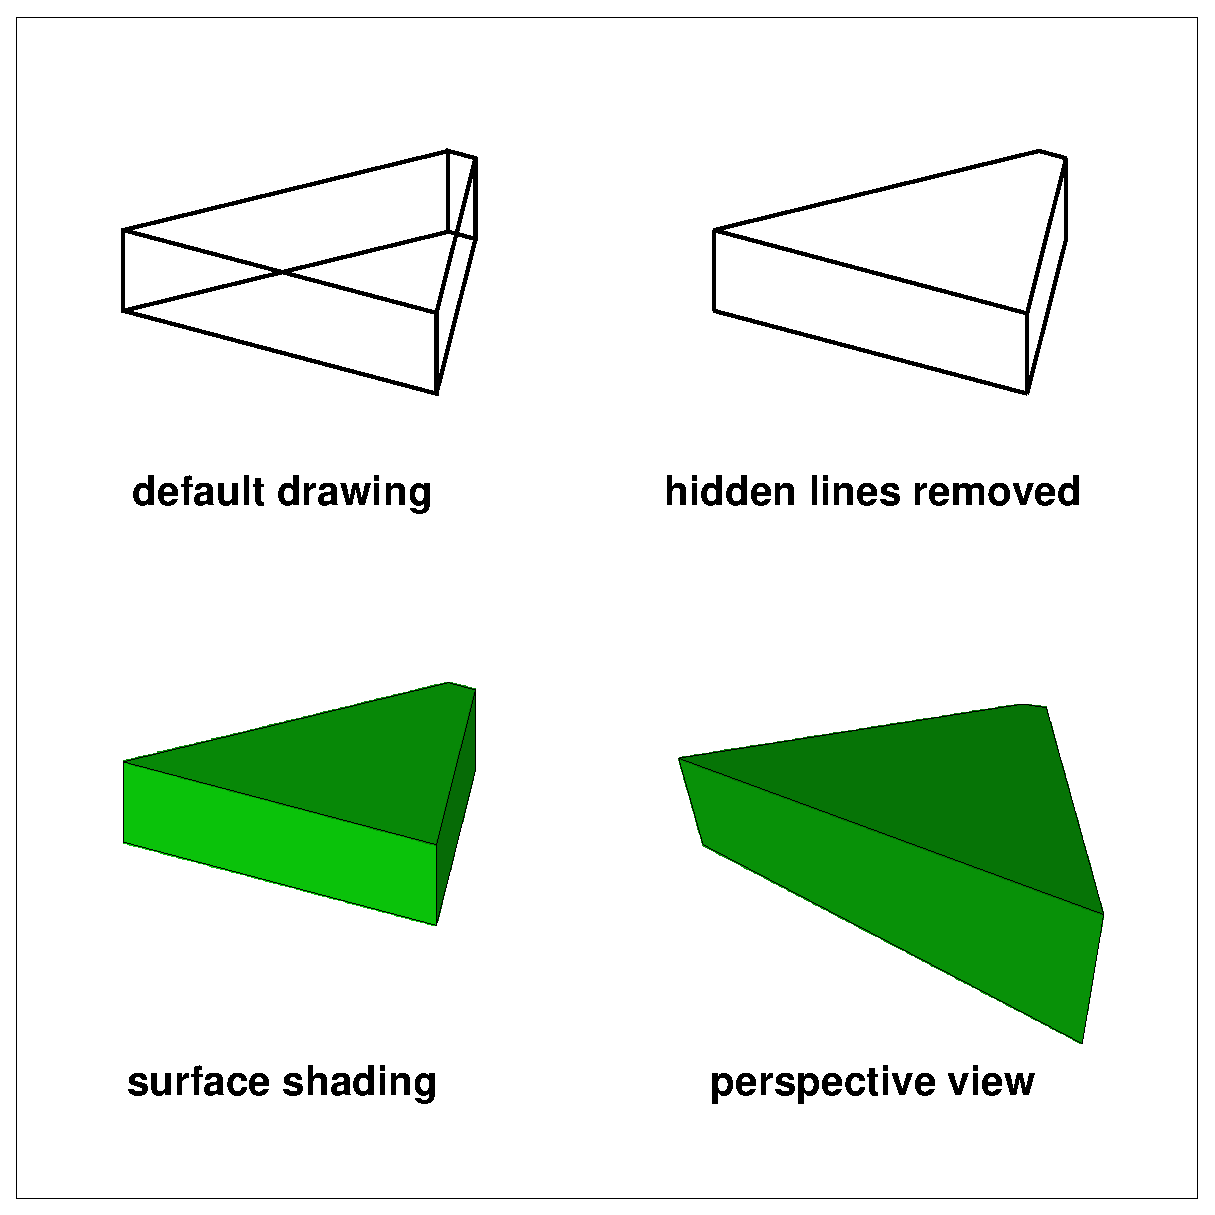
\epsfig{file=eps/draw110-1.eps,width=10cm}
      \caption{Examples of use of {\tt GDRAW}}
      \label{draw110-1}
\end{figure}

Drawing with hidden line removal and surface fill shading is also possible, 
but the drawing time may increase substantially for complicated 
objects.

When using the interactive interface it is possible to {\it cut}
the object to be drawn with {\it cutting} volumes (command {\tt CVOL}).
This is particularly
useful to visualise the contents of an object drawn with hidden line removal.
Another feature which is available only interactively is the possibility
to draw each decendant of a volume shifted along the axis which goes from the
centre of the local coordinate system to the centre of gravity of
the descendant itself. This again is useful to improve the visibility of the
details of a complicated setup (command {\tt BOMB}). Please see the interactive
interface description for more information on this part.

\begin{DLtt}{MMMMM}
\item[CHNAME]  ({\tt CHARACTER*4}) volume name.
\item[THETA] ({\tt REAL}) theta angle between the line of sight and the
Z axis of {\tt MA}ster {\tt R}eference {\tt S}ystem ({\tt MARS}).
\item[PHI]   ({\tt REAL}) phi angle between the projection of the line 
of sight on plane {\tt X  Y} and the {\tt X} axis of {\tt MARS}.
\item[PSI]   ({\tt REAL}) psi angle by which the projected image will 
be rotated on the screen plane.
\item[U0]    ({\tt REAL}) u coordinate on the screen of the volume origin.
\item[V0]    ({\tt REAL}) v coordinate on the screen of the volume origin.
\item[SU]    ({\tt REAL}) scale factor for u coordinates.
\item[SV]    ({\tt REAL}) scale factor for v coordinates.
\end{DLtt}

%%%%%%%%%%%%%%%%%%%%%%%%%%%%%%%%%%%%%%%%%%%%%%%%%%%%%%%%%%%%%%%%%%%
%                                                                 %
%  GEANT manual in LaTeX form                                     %
%                                                                 %
%  Michel Goossens (for translation into LaTeX)                   %
%  Version 1.00                                                   %
%  Last Mod. Jan 24 1991  1300   MG + IB                          %
%                                                                 %
%%%%%%%%%%%%%%%%%%%%%%%%%%%%%%%%%%%%%%%%%%%%%%%%%%%%%%%%%%%%%%%%%%%  
\Origin{P.Zanarini}
\Documentation{P.Zanarini, F.Carminati}
\Submitted {01.01.86}   \Revised{11.12.92}
\Version{Geant 3.15}\Routid{DRAW115}
\Makehead{Drawing a Volume Projection view -- Case 2}
\Shubr{GDRVOL}{(NNAMS,CHNAMS,LNUMBS,NRS,THETA,PHI,PSI,U0,V0,SU,SV)}
Draws an orthographic parallel projection or a perspective projection 
(depending on the option chosen via \Rind{GDOPT}) of the volume 
{\tt CHNAMS(N),LNUMBS(N)} with all its descendants, at the position 
{\tt U0,V0} (user coordinates), with the scale factors {\tt SU} and 
{\tt SV}. 
The object is seen from {\tt THETA} and {\tt PHI} angles, 
and the resulting 2D projection is also rotated by an angle {\tt PSI} 
on the screen plane. These parameters, as well as zoom parameters set 
by \Rind{GDZOOM}, define the current {\it view parameters}, and they are 
copied in \FCind{/GCDRAW/}.  Attributes like colour, fill area, line 
width, line style, visibility, etc. can be set by the \Rind{GSATT} 
routine for {\tt CHNAMS(N)} and or its descendants {\tt [GEOM 500]}.
This routine differs from \Rind{GDRAW} in the following aspects:
\begin{itemize}
\item  The object to be drawn is identified by a full path. This gives 
the possibility of drawing a particular copy or division of a volume, or 
even a volume that has more than one mother in the geometry tree.
{\tt CHNAMS(1),...,CHNAMS(N)} contain the volume names and
{\tt LNUMBS(1),...,LNUMBS(N)}, the volume numbers defining the path 
to go from the top volume to the one to be drawn.
\item  The object can be drawn either with respect to the
{\tt MA}ster {\tt R}eference {\tt S}ystem ({\tt NRS=0}) or with respect 
to its {\tt D}augther {\tt R}eference {\tt S}ystem (i.e. the Local R.S.); 
in the first case it is drawn in its position in the real world, while 
in the second one it is drawn like \Rind{GDRAW} would do.
\item  In this latter case, track and hit points will be
drawn with respect to the {\tt DRS} of the volume last
drawn by this routine, and not with respect to the
{\tt MARS} as is done normally (to reset to the normal
case a call with {\tt NRS=0} or {\tt NNAMS=0} is required).
\end{itemize}
\begin{DLtt}{MMMMMM}
\item[NNAMS]     ({\tt INTEGER}) number of elements {\tt levels} in the 
arrays {\tt CHNAMS, LNUMBS}. The bottom volume of this path is also the 
one that is actually drawn;
\item[CHNAMS]   ({\tt CHARACTER*4}) array of volume name (dimensioned 
at least to {\tt NNAMS});
\item[LNUMBS]   array of volume numbers (dimensioned at least to {\tt NNAMS});
\item[NRS]    reference system used:
\begin{DLtt}{MMMMM}
\item[NRS$=$0] to have the volume(s) drawn with respect to the {\tt MARS} 
\item[NRS$\neq$0] to have the volume(s) drawn with respect to the {\tt DRS}
\end{DLtt}
\item[THETA]   $\theta$ angle between the line of sight and the
                Z  axis of {\tt MARS};
\item[PHI]    $\phi$ angle between the projection of the line of sight
              on plane {\tt X Y} and the {\tt X} axis of {\tt MARS}
\item[PSI]   $\psi$ angle by which the projected image will
             be rotated on the screen plane
\item[U0]    u coordinate on the screen of the volume origin
\item[V0]    v  coordinate on the screen of the volume origin
\item[SU]   scale factor for u coordinates
\item[SV]   scale factor for v coordinates
\end{DLtt}
 
Two examples of use of \Rind{GDRVOL} are shown in fig~\ref{fg:draw115-1} and
\ref{fg:draw115-2}.

\begin{figure}[hbt]
      \centering
      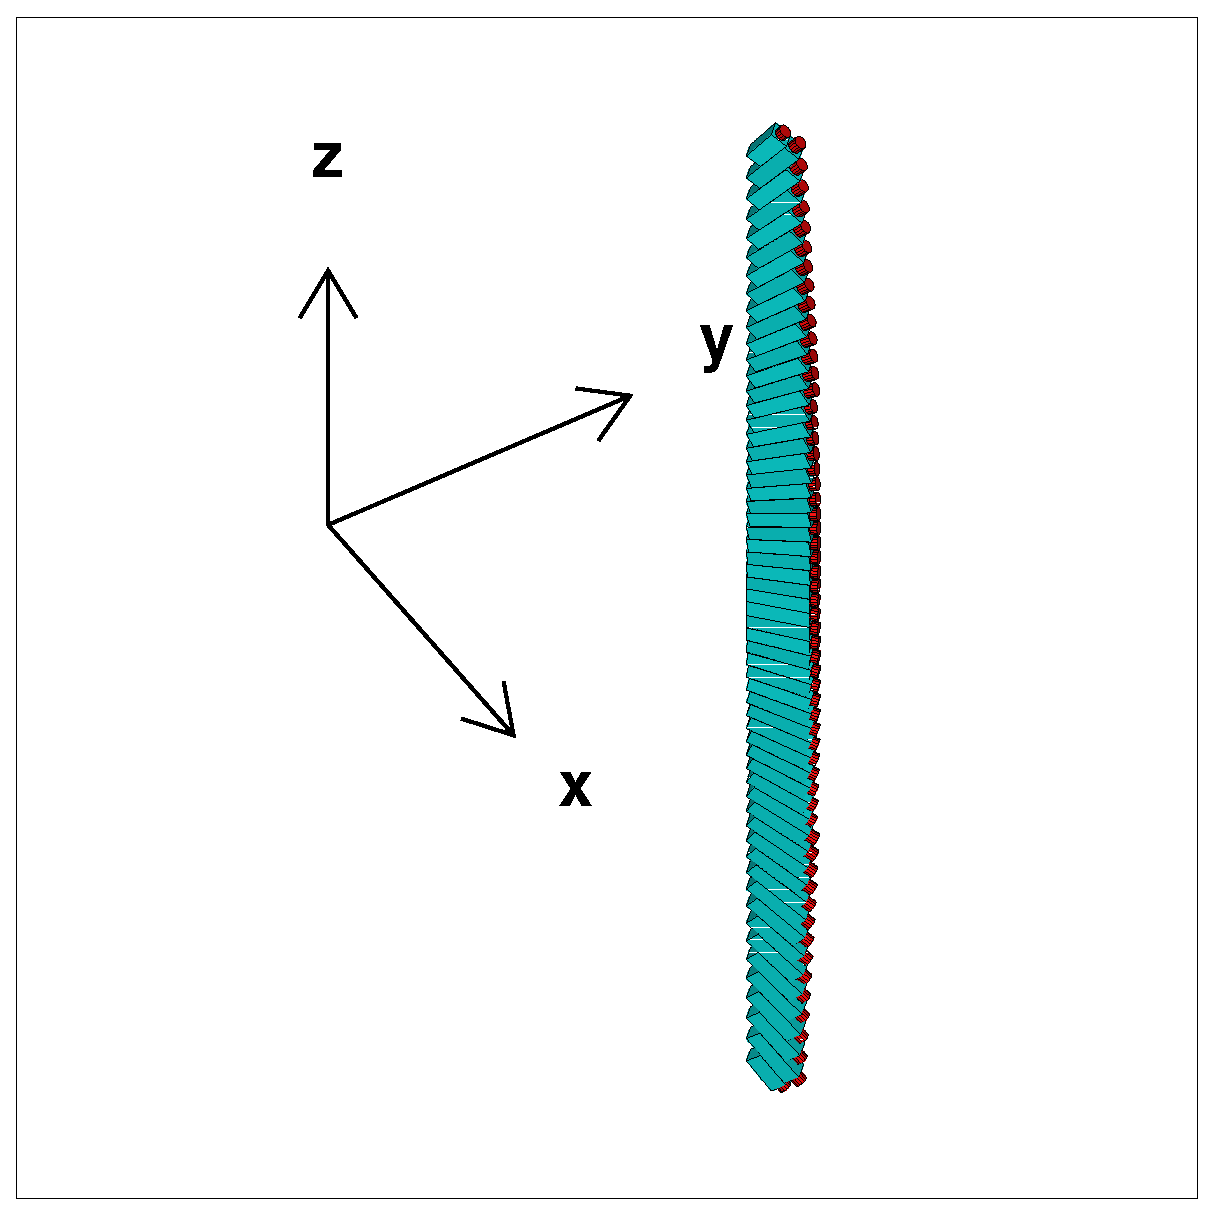
\epsfig{file=eps/draw115-1.eps,width=12cm}

\begin{verbatim}
       CHARACTER*4 CHNAMS(5)
       INTEGER LNUMBS(5)
       DATA CHNAMS/'OPAL','BRL-','EB  ','EBB ','EBP '/
       DATA LNUMBS/    1 ,    1 ,    1 ,    1 ,   20 /
       .
       .
       .
       NRS=0
       CALL GDRVOL(5,CHNAMS,LNUMBS,NRS,80.,135.,0.,13.,10.,0.03,0.03)
       CALL GDAXIS(0.,0.,0.,200.)
C      CALL GDXYZ(0)
\end{verbatim}

     \caption{Example of use of {\tt GDRVOL} in the MAster Reference System}
     \label{fg:draw115-1}


\end{figure}


\begin{figure}[hbt]
     \centering
     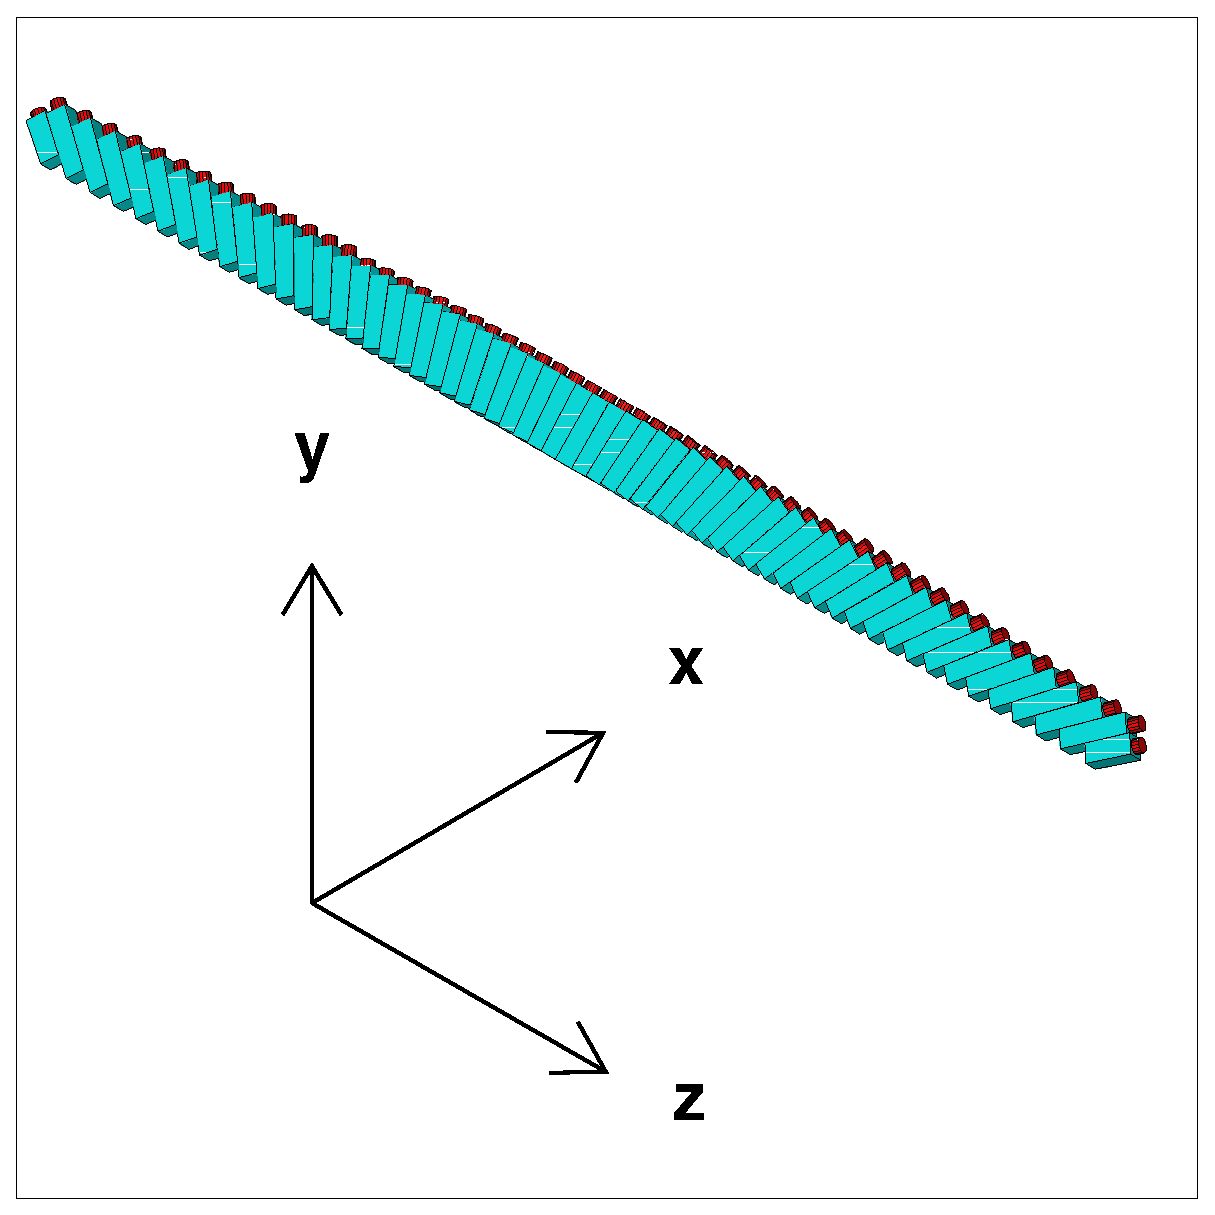
\epsfig{file=eps/draw115-2.eps,width=12cm}

\begin{verbatim}
      CHARACTER*4 CHNAMS(5)
      INTEGER LNUMBS(5)
      DATA CHNAMS/'OPAL','BRL-','EB  ','EBB ','EBP '/
      DATA LNUMBS/    1 ,    1 ,    1 ,    1 ,   20 /
      .
      .
      .
      NRS=1
      CALL GDRVOL(5,CHNAMS,LNUMBS,NRS,55.,135.,0.,5.,5.,0.035,0.035)
      CALL GDAXIS(0.,0.,0.,200.)
C     CALL GDXYZ(0)
\end{verbatim}

\caption{Example of use of {\tt GDRVOL} in the Daughter Reference System}
\label{fg:draw115-2}
\end{figure}
 

%%%%%%%%%%%%%%%%%%%%%%%%%%%%%%%%%%%%%%%%%%%%%%%%%%%%%%%%%%%%%%%%%%%
%                                                                 %
%  GEANT manual in LaTeX form                              %
%                                                                 %
%  Michel Goossens (for translation into LaTeX)                   %
%  Version 1.00                                                   %
%  Last Mod. Jan 24 1991  1300   MG + IB                          %
%                                                                 %
%%%%%%%%%%%%%%%%%%%%%%%%%%%%%%%%%%%%%%%%%%%%%%%%%%%%%%%%%%%%%%%%%%%
\Origin {P.Zanarini}
\Documentation{P.Zanarini}
\Submitted{15.05.84}       \Revised{10.12.93}
\Version{Geant 3.16}\Routid{DRAW120}
\Makehead{Draw a volume cut view}
\Shubr{GDRAWX}{(CHNAME,CUTTHE,CUTPHI,CUTVAL,THETA,PHI,U0,V0,SU,SV)}
 
\begin{DLtt}{MMMMMMMM}
\item[CHNAME] ({\tt CHARECTER*4}) name of volume;
\item[CUTTHE] ({\tt REAL}) $\theta$ angle of the line normal to the cut plane;
\item[CUTPHI] ({\tt REAL}) $\phi$ angle of the line normal to the cut plane;
\item[TETHA]  ({\tt REAL}) viewing angle $\theta$;
\item[PHI]    ({\tt REAL}) viewing angle $\phi$;
\item[U0]     ({\tt REAL}) u coordinate on the screen of the volume origin;
\item[V0]     ({\tt REAL}) v  coordinate on the screen of the volume origin;
\item[SU]     ({\tt REAL}) scale factor for u  coordinates;
\item[SV]     ({\tt REAL}) scale factor for v   coordinates.
\end{DLtt}

Draws a {\it cut view} of the volume {\tt CHNAME}
with all its {\it visible} descendants, i.e. draws their intersection with
the cut plane normal to the axis
given by the angles {\tt CUTTHE, CUTPHI} at the distance {\tt CUTVAL}
from the origin.
The view point is defined by the angles {\tt THETA, PHI}.
{\tt U0, V0, SU, SV} have the same meaning as in \Rind{GDRAW}.
These {\it view parameters}, as well as zoom parameters set by \Rind{GDZOOM}
are copied in \FCind{/GCDRAW/}.

Attributes like colour, surface fill, line width, line style, visibility, etc.
can be set by the \Rind{GSATT} routine for {\tt CHNAME}
and its descendants {\tt [GEOM500]}.
 
\Shubr{GDRAWC}{(CHNAME,IAX,CUTVAL,U0,V0,SU,SV)}
 
\begin{DLtt}{MMMMMMMM}
\item[CHNAME] ({\tt CHARECTER*4}) name of volume;
\item[IAX]  ({\tt INTEGER}) axis of the cut (1=X, 2=Y, 3=Z);
\item[U0]   ({\tt REAL}) u coordinate on the screen of the volume origin;
\item[V0]   ({\tt REAL}) v coordinate on the screen of the volume origin;
\item[SU]   ({\tt REAL}) scale factor for u coordinates;
\item[SV]   ({\tt REAL}) scale factor for v coordinates.
\end{DLtt}

This routine is a special case of the previous \Rind{GDRAWX}.
Here the cut plane is normal to one of the main axes ({\tt IAX})
and placed at a distance {\tt CUTVAL} from the origin.
The view-point is along the same axis.
 
Fig.~\ref{fg:draw120-1} gives an example of utilisation of 
\Rind{GDAXIS}, \Rind{GDRAW} and \Rind{GDRAWX}. Fig.~\ref{fg:draw120-2}
gives an example of use of \Rind{GDRAWC}.

\begin{figure}[hbt]
     \centering
     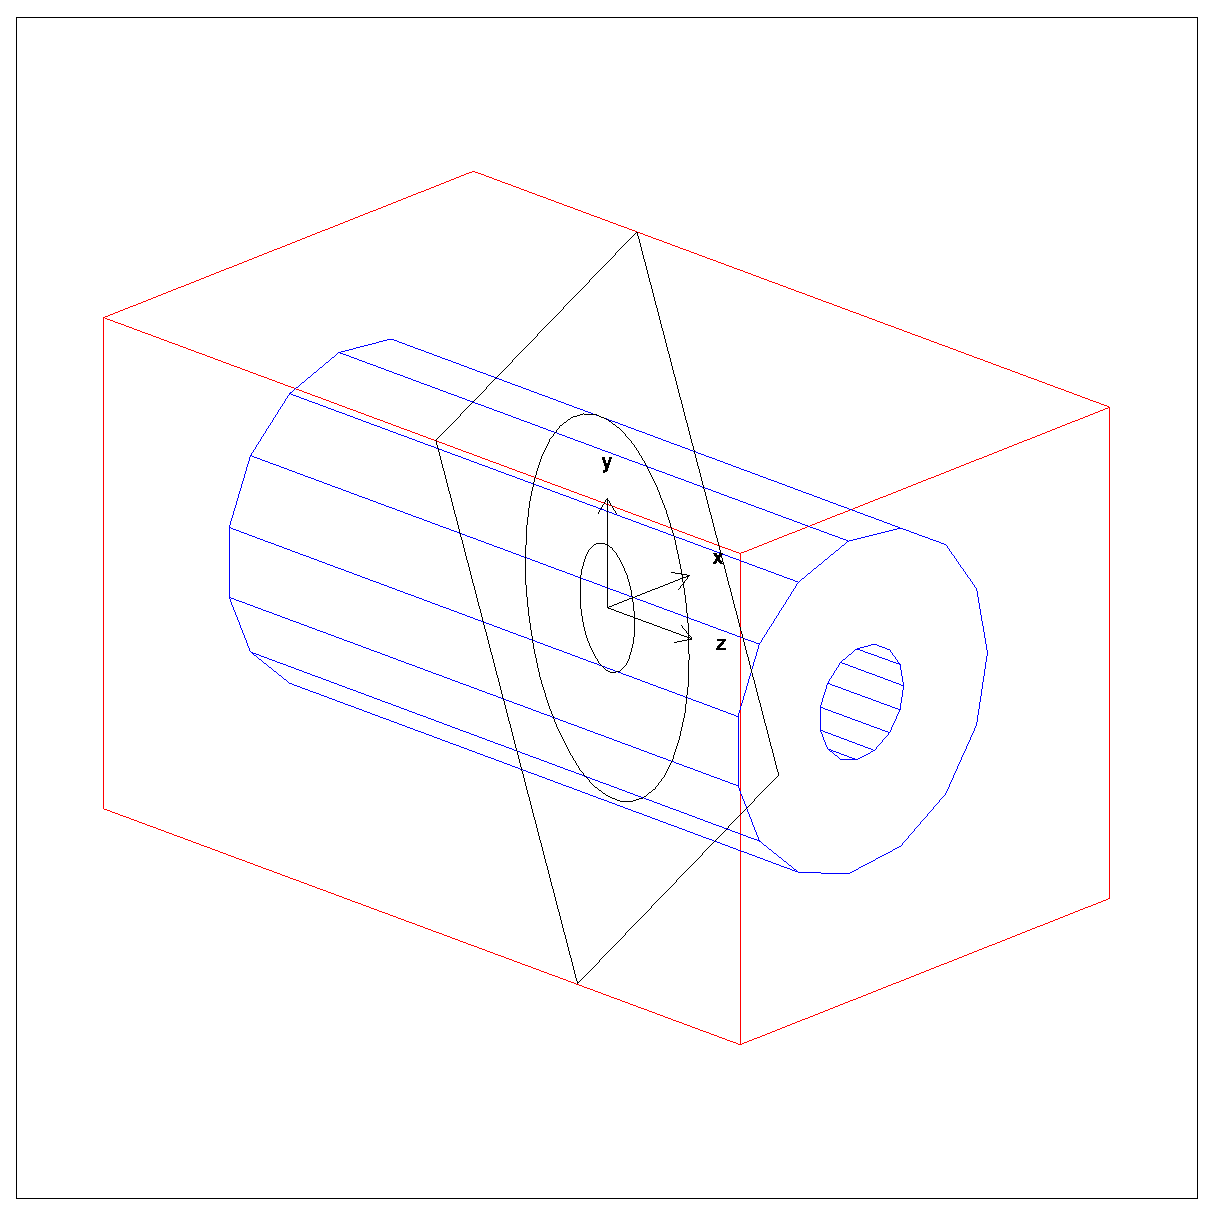
\epsfig{file=eps/draw120-1.eps,width=14cm}
\begin{verbatim}
      CALL GDOPT('HIDE','ON')
      CALL GSATT('NBOX','COLO',2.)
      CALL GSATT('NTUB','COLO',4.)
      CALL GDRAW('NBOX',50.,150.,0.,10.,10.,0.01,0.01)
      CALL GDRAW('NTUB',50.,150.,0.,10.,10.,0.01,0.01)
      CALL GDOPT('HIDE','OFF')
      CALL GSATT('*','COLO',1.)
      CALL GDRAWX('NBOX',30.,40.,0.,50.,150.,10.,10.,0.01,0.01)
      CALL GDAXIS(0.,0.,0.,200.)
\end{verbatim}
     \caption{Example of utilisation of 
{\tt GDAXIS}, {\tt GDRAW} and {\tt GDRAWX}}
     \label{fg:draw120-1}
\end{figure}
 
\begin{figure}[hbt]
     \centering
     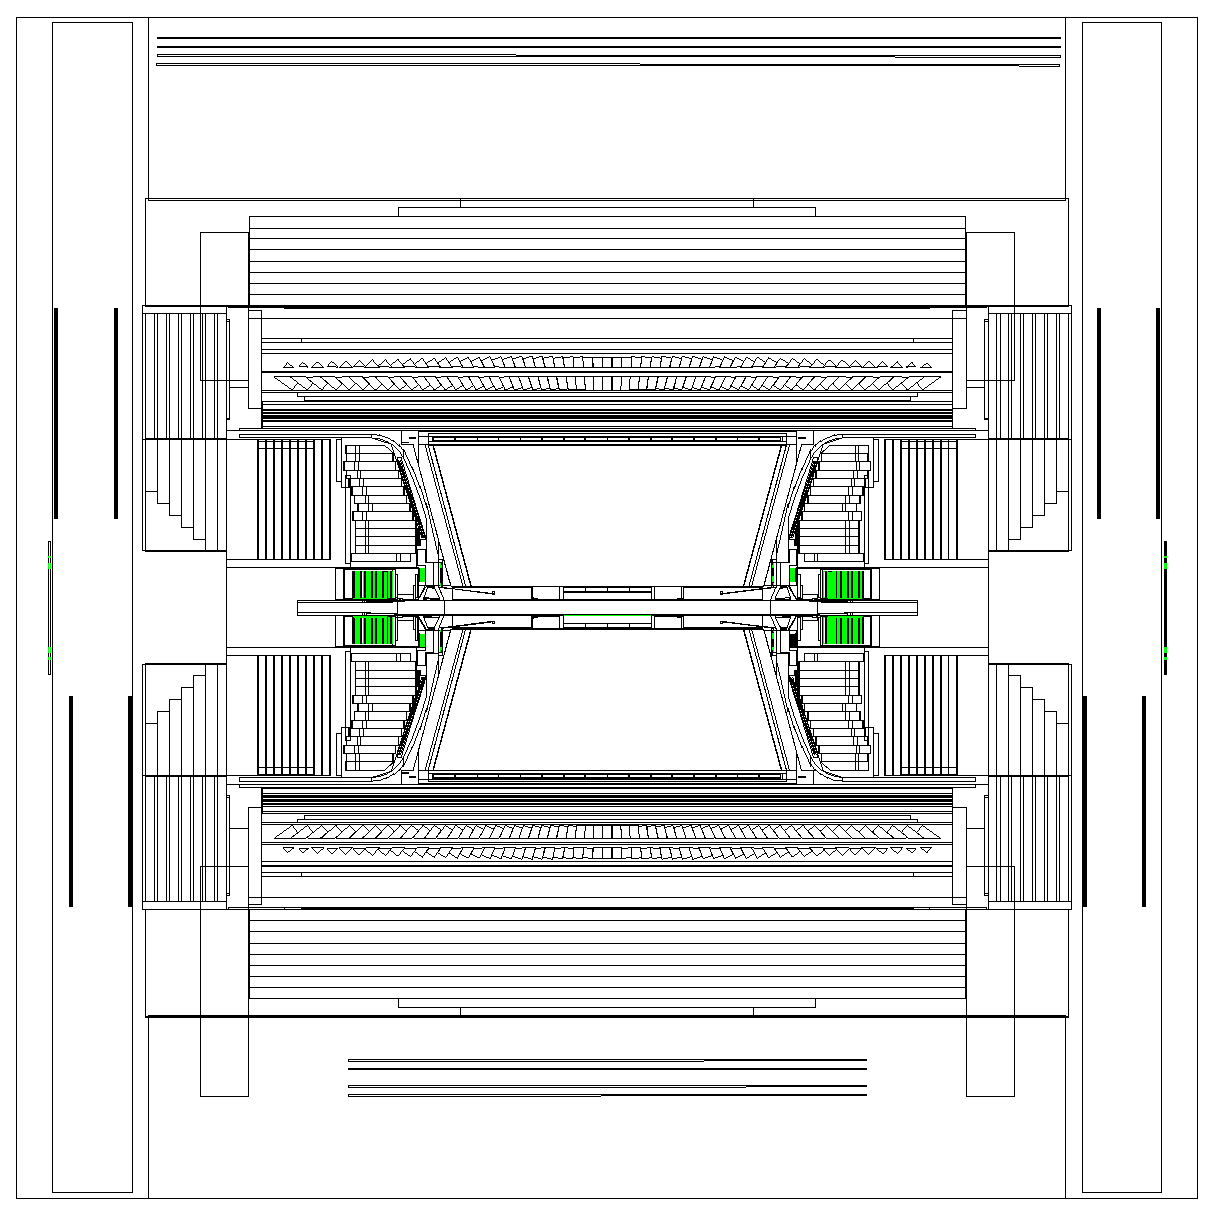
\epsfig{file=eps/draw120-2.eps,width=14cm}
\begin{verbatim}
      CALL GDRAWC('OPAL',2,0.,10.,10.,0.01,0.01)
\end{verbatim}
     \caption{Example of utilisation of {\tt GDRAWC}}
     \label{fg:draw120-2}
\end{figure}

%%%%%%%%%%%%%%%%%%%%%%%%%%%%%%%%%%%%%%%%%%%%%%%%%%%%%%%%%%%%%%%%%%%
%                                                                 %
%  GEANT manual in LaTeX form                              %
%                                                                 %
%  Michel Goossens (for translation into LaTeX)                   %
%  Version 1.00                                                   %
%  Last Mod. Jan 24 1991  1300   MG + IB                          %
%                                                                 %
%%%%%%%%%%%%%%%%%%%%%%%%%%%%%%%%%%%%%%%%%%%%%%%%%%%%%%%%%%%%%%%%%%%
\Origin {R.Brun, P.Zanarini}
\Documentation{P.Zanarini}
\Submitted{15.05.84}             \Revised{11.12.92}
\Version{Geant 3.16}\Routid{DRAW130}
\Makehead{Draw Particle Trajectories}
\section{Visualisation of particle trajectories}
The tracks generated by the tracking package, and optionally stored
in the data structure {\tt JXYZ}, can be displayed by the routine \Rind{GDXYZ}
(corresponding to the interactive command {\tt DXYZ}).
 
The names of the particles and or the track numbers can be added
by the routine \Rind{GDPART} (corresponding to the interactive command 
{\tt DPART}).
 
A special routine has been provided to visualise the tracks during the
transport process
(\Rind{GDCXYZ}), that could be called for instance by \Rind{GUSTEP}.
That routine shows the tracks while they are transported
by the tracking package of {\tt GEANT}, providing a useful interactive
debugging tool.

\Shubr{GDXYZ}{(ITRA)}
 
Draws track number {\tt ITRA} for which space points have been stored in bank
{\tt JXYZ} via calls to the routine \Rind{GSXYZ}. The view parameters are 
taken from \FCind{/GCDRAW/}.
\begin{DLtt}{MMM}
\item[ITRA] ({\tt INTEGER}) track number (if 0 all tracks are taken)
\end{DLtt}
The colour and line style corresponds to the track type :
\begin{center}
\newcommand{\HSP}{\hspace{3mm}}
\newcommand{\HDD}{\makebox[2mm][c]{.}}
\newcommand{\HHH}{\makebox[2mm][c]{-}}
\newcommand{\HSPD}{\HSP\HDD\HSP\HDD\HSP\HDD\HSP\HDD\HSP\HDD\HSP\HDD}
\newcommand{\HSPH}{\HSP\HHH\HSP\HHH\HSP\HHH\HSP\HHH\HSP\HHH\HSP\HHH}
\begin{tabular}{llp{3cm}}
(blue)  & dotted line for gammas
                                                    & \dotfill \\
(red)   & solid line for charged particles (except muons)
                                                    & \hrulefill \\
(black) & blank/dotted line for neutral hadrons or neutrinos
                                                    & \HSPD \\
(green) & dashed line for muons
                                                    & \HSPH \\
(yellow) & dotted line for \v{C}erenkov photons
                                                    & \dotfill
\end{tabular}\end{center}
\Shubr{GDPART}{(ITRA,ISEL,SIZE)}
Draws the particle names and/or the track numbers
of track {\tt ITRA}, supposing that its space points had been stored in 
the bank {\tt JXYZ} via the routine \Rind{GSXYZ}.
At present only primary tracks are displayed by \Rind{GDPART}
and their name or number is written at the end the track trajectory.
The view parameters are taken from \FCind{/GCDRAW/}.
\begin{DLtt}{MMMM}
\item[ITRA]  ({\tt INTEGER}) Track number (if 0 all tracks are taken)
\item[ISEL]  ({\tt INTEGER}) \\
             {\tt ISEL=x1} draws the track number, \\
             {\tt ISEL=1x} draws the particle name, \\
             {\tt ISEL=11} draws both.
\item[SIZE]  ({\tt REAL}) Character size in cm.
\end{DLtt}
\Shubr{GDCXYZ}{}
If \Rind{GDCXYZ} is called at tracking time (for instance by
\Rind{GUSTEP}), it draws the tracks while tracking is performed,
at the same time as
they are generated by the tracking package of {\tt GEANT}.
This is a very
useful interactive debugging tool. The line style is the same as for
\Rind {GDXYZ}.
The view parameters are taken from \FCind{/GCDRAW/}.

Here we give an example of the use of \Rind{GDPART}:
 
\begin{verbatim}
 CALL GSATT('HB','FILL',3)
 CALL GSATT('HE','FILL',1)
 - - - - -
 - - - - -
 
 CALL GDRAWC('OPAL',2,5.,10.,10.,0.013,0.013)
 CALL GDXYZ(0)
 CALL GDPART(0,11,0.25)
\end{verbatim}
 

%%%%%%%%%%%%%%%%%%%%%%%%%%%%%%%%%%%%%%%%%%%%%%%%%%%%%%%%%%%%%%%%%%%
%                                                                 %
%  GEANT manual in LaTeX form                                     %
%                                                                 %
%  Michel Goossens (for translation into LaTeX)                   %
%  Version 1.00                                                   %
%  Last Mod. Jan 24 1991  1300   MG + IB                          %
%                                                                 %
%%%%%%%%%%%%%%%%%%%%%%%%%%%%%%%%%%%%%%%%%%%%%%%%%%%%%%%%%%%%%%%%%%%
\Origin{R.Brun, W.Gebel, P.Zanarini}
\Documentation{S.Giani, F.Carminati}
\Submitted{07.03.84}    \Revised{11.12.92}
\Version{Geant 3.15}\Routid{DRAW140}
\Makehead{Drawing Track Hits in Sensitive Detectors}
The hits generated by the tracking package and stored in the
data structure {\tt JHITS} can be displayed by the following routines:
\begin{enumerate}
\item draw one hit (\Rind{GDAHIT}); called by the user;
\item draw all the hits of trajectory type sets/ detectors (\Rind{GDHITS});
\item draw all the hits of calorimeter type sets/ detectors (\Rind{GDCHIT}).
\end{enumerate}

Different symbols for each subdetector can be used, chosen among
hardware characters (dots), software crosses, or from the {\tt HPLOT} table
of software characters.
The size of the software characters and crosses is given as an argument
to \Rind{GDAHIT} and \Rind{GDHITS}, while it is computed as a function of 
the hits value in \Rind{GDCHIT}.

The option {\tt H} of the interactive \Rind{MOVE} command gives the 
possibility
to rotate, zoom and translate in real time the hits stored for one event.
This allow a 3D display of the event where it is possible to pick one hit 
with the mouse and have the hit values printed.  The interactive 
command \Rind{LENS} allows a detailed visual scanning of the 
hits displayed (see the interactive section).   

\Shubr{GDHITS}{(CHUSET,CHUDET,ITRA,ISYMB,SSYMB)}
Draws the hit points as stored by \Rind{GSAHIT,} which were
generated by track {\tt ITRA} in detector {\tt CHUDET} of set {\tt CHUSET},
with the currently selected view parameters in \FCind{/GCDRAW/}.
The character plotted at each point may be chosen via {\tt ISYMB}:
 
\begin{tabular}{l@{\hspace{2cm}}l@{\hspace{3cm}}r}
 -1     &  (small) hardware points            & (fast)      \\
  0     &  software crosses                   & (default)   \\
840/850 &  empty/full circles                 & (slow)      \\
841/851 &  empty/full squares                 & (slow)      \\
842/852 &  empty/full triangles (up)          & (slow)      \\
843/853 &  empty diamond/full triangle (down) & (slow)      \\
844/854 &  empty/full stars                   & (slow)      \\
\end{tabular}
 
More information on the meaning of the {\tt ISIMB} value can be found in the 
{\tt HPLOT} manual\cite{bib-HPLOT}. Any value for {\tt ISYMB} which is not
in the above table is equivalent to option 0. Except for {\tt ISYMB = -1},
the size of the character can be chosen by {\tt SSYMB}.
On the 2D projection on the screen one can distinguish which
set/detector a given track passes, by drawing different symbols for the
hits in different sets/detectors. The size of these symbols may then
be chosen to suit the scale of the total picture (detectors and tracks).

\begin{figure}[hbt]
     \centering
     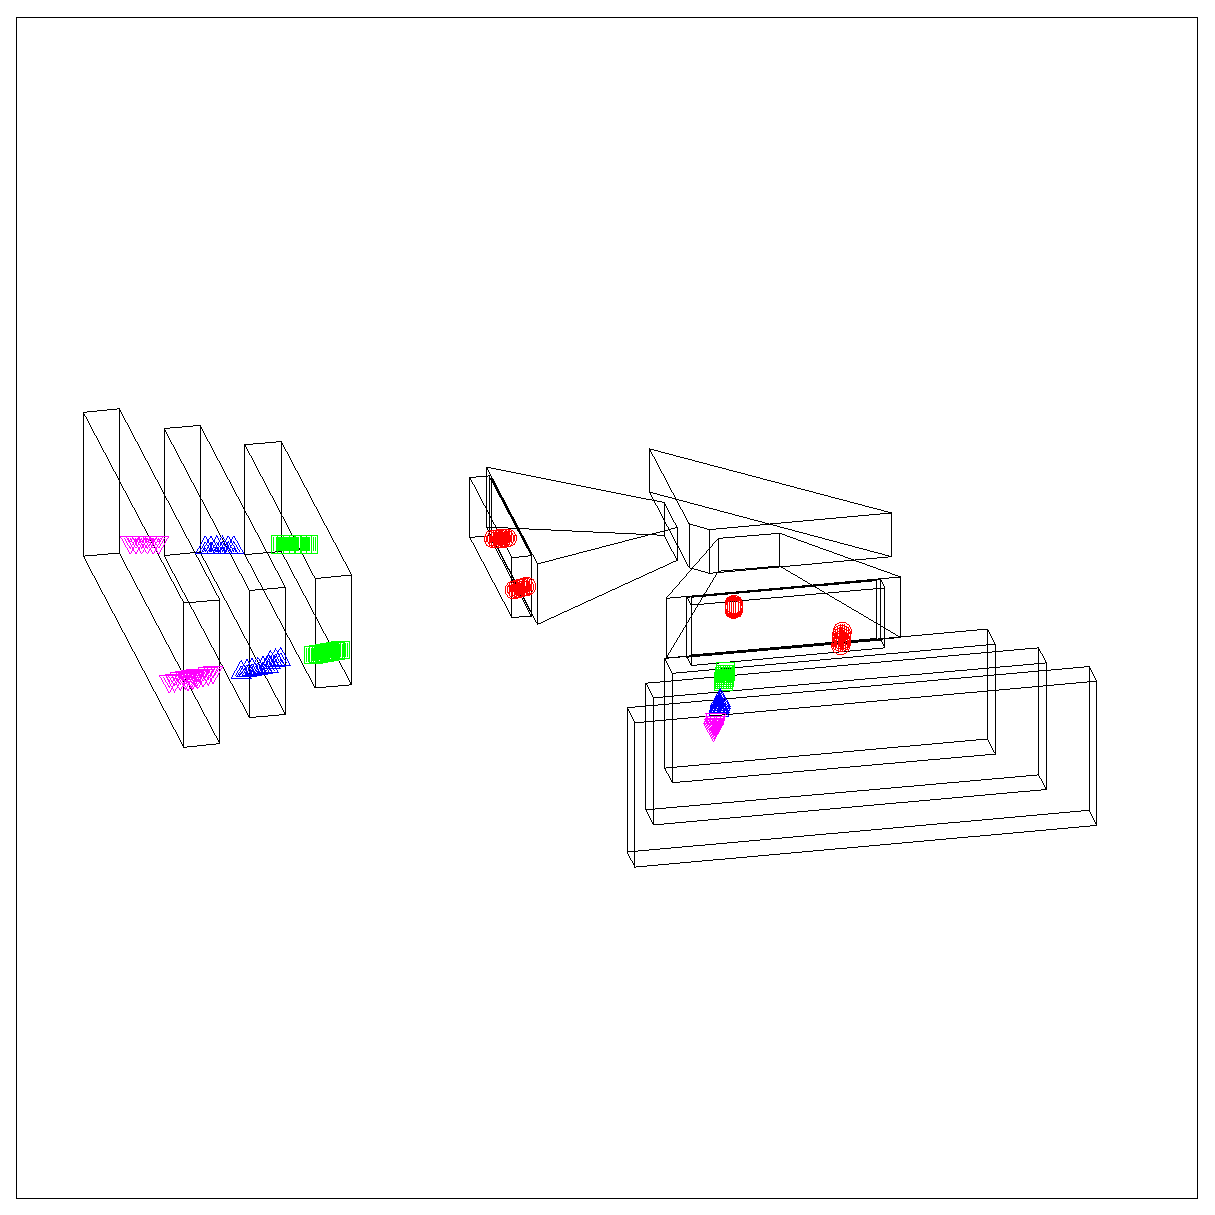
\epsfig{file=eps/draw140-1.eps,width=10cm}

\begin{verbatim}
 CALL GDRAW('CAVE',40.,40.,0.,10.,10.,.04,.04)
 CALL IGSET('TXCI',2.)
 CALL GDHITS('DRFT','FSP ',0,850,.3)
 CALL IGSET('TXCI',3.)
 CALL GDHITS('DRFT','RSP1',0,851,.3)
 CALL IGSET('TXCI',4.)
 CALL GDHITS('DRFT','RSP2',0,852,.3)
 CALL IGSET('TXCI',5.)
 CALL GDHITS('DRFT','RSP3',0,853,.3)
\end{verbatim}

     \caption{example of use of {\tt GDHITS}}
     \label{fg:draw140-1}
\end{figure}

{\bf Note:}
It is obligatory for the use of this routine that the spatial
{\tt MARS} (MAster Reference System) current coordinates of the hits are stored
as the first 3 elements of the hit {\tt [HITS200]}.
\begin{DLtt}{MMMMM}
\item[CHUSET] ({\tt CHARACTER*4}) user set identifier (if '*' all sets are taken)
\item[CHUDET] ({\tt CHARACTER*4}) user detector identifier (if '*' all 
detectors are taken)
\item[ITRA]   ({\tt INTEGER}) number of selected track (if 0 all tracks are taken)
\item[ISYMB]  ({\tt INTEGER}) character selection number (see table above)
\item[SSYMB]  ({\tt REAL}) size of characters in cm (if 0, a default of 
0.1 is taken)
\end{DLtt}
\Shubr{GDCHIT}{(CHUSET,CHUDET,ITRA,ISYMB,SIZMAX,IHIT,HITMIN,HITMAX)}
Draws the hit points as stored by \Rind{GSCHIT}, which were
generated by track {\tt ITRA} in detector {\tt CHUDET} of set {\tt CHUSET},
with the currently selected view parameters in \FCind{/GCDRAW/}.
Except for {\tt ISYMB = -1} the size of the character
is chosen as a function of {\tt HITS(IHIT)}:
\begin{center}
\ttfamily SIZE = sizmax * ( hits(ihit) - hitmin ) / hitmax
\end{center}

{\bf Note:}
It is obligatory for the use of this routine that the spatial
{\tt MARS} ({\tt MA}ster {\tt R}eference {\tt S}ystem) current coordinates 
of the hits are stored as the first 3 elements of the hit {\tt [HITS200]}.
\begin{DLtt}{MMMMM}
\item [SIZMAX]   ({\tt REAL}) maximum character size in cm
\item [IHIT]     ({\tt INTEGER}) {\tt HITS(IHIT)} contains the calorimeter 
hit value. {\tt IHIT>3}, and the first three elements are supposed to
contain the space position of the hit
\item [HITMIN]    ({\tt REAL}) minimum boundary of {\tt HITS(IHIT)}
\item[HITMAX]     ({\tt REAL}) maximum boundary of {\tt HITS(IHIT)}
\end{DLtt}
\Shubr{GDAHIT}{(X,Y,Z,ISYMB,SSYMB)}
Draws one hit point at coordinates {\tt X, Y, Z}. This routine is useful
when the user wants only to display but not to store the hits.
The first three arguments are the position of the hit in the {\tt MARS},
and the last two arguments have the same meaning as the similar 
arguments in GDHITS.
\begin{DLtt}{MM}
\item [X]  ({\tt REAL})       x coordinate in {\tt MARS} of the hit point
\item [Y]  ({\tt REAL})       y coordinate in {\tt MARS} of the hit point
\item [X]  ({\tt REAL})       z coordinate in {\tt MARS} of the hit point
\end{DLtt}

An example of use of the hits drawing routines is given in fig~\ref{fg:draw140-1}.
%\begin{verbatim}
%SUBROUTINE GUTREV
% - - - - -
% CALL GDOPT('THRZ','ON ')
% CALL GDRAWC('OPAL',2,5.,10.,10.,0.013,0.013)
% CALL GTREVE
% END
% 
% SUBROUTINE GUSTEP
% - - - - -
% CALL GDCXYZ
% - - - - -
% END
% 
% CALL GDOPT('THRZ','ON  ')
% CALL GDRAWC('OPAL',2,5.,10.,10.,0.013,0.013)
% CALL GDCHIT('EB  ',0,0,841,1.,6,0.,0.5)
% CALL GDCHIT('EE  ',0,0,841,1.,6,0.,0.5)
% CALL GDCHIT('HB  ',0,0,851,1.,5,0.,0.5)
% CALL GDCHIT('HE  ',0,0,851,1.,5,0.,0.5)
% CALL GDHITS('CJ  ',0,0,0,0.01)
% CALL GDHITS('CV  ',0,0,0,0.01)
% CALL GDHITS('CZ  ',0,0,0,0.01)
% CALL GDHITS('F   ',0,0,853,0.1)
% CALL GDHITS('HP  ',0,0,840,0.2)
% CALL GDHITS('ME  ',0,0,842,0.2)
% CALL GDHITS('MB  ',0,0,842,0.2)
%\end{verbatim}
% 
% 

%%%%%%%%%%%%%%%%%%%%%%%%%%%%%%%%%%%%%%%%%%%%%%%%%%%%%%%%%%%%%%%%%%%
%                                                                 %
%  GEANT manual in LaTeX form                                     %
%                                                                 %
%  Michel Goossens (for translation into LaTeX)                   %
%  Version 1.00                                                   %
%  Last Mod. Jan 24 1991  1300   MG + IB                          %
%                                                                 %
%%%%%%%%%%%%%%%%%%%%%%%%%%%%%%%%%%%%%%%%%%%%%%%%%%%%%%%%%%%%%%%%%%%
\Origin{P.Zanarini}   
\Revision{S.Giani}
\Documentation{P.Zanarini, S.Giani}
\Submitted{15.01.84}            \Revised{10.12.93}
\Version{Geant 3.16}            \Routid{DRAW210}

\Makehead{Drawing the geometrical tree}
The geometrical tree is a hierarchical representation of the 
structure of the detector, based on the mother-daughter
relationship among the various volumes composing it. The \Rind{GDTREE} 
routine (corresponding to the {\tt DTREE} interactive command) allows 
the drawing of the logical tree, displaying name, multiplicity 
and other information about the volumes.

\Shubr{GDTREE}{(CHNAME,LEVMAX,ISEL)}
\begin{DLtt}{MMMMMMMM}
\item[CHNAME]  ({\tt CHARACTER*4}) volume name;
\item[LEVMAX]  ({\tt INTEGER}) depth levels (if 0 all levels are taken) 
default is 3;
\item[ISEL]    ({\tt INTEGER}) used to select options in the picture of the tree:
\begin{DLtt}{MMMMMM}
\item[~~~~0] only the node name is drawn;
\item[xxxx1] multiplicity is added: 
\begin{itemize}
\item each node that has been positioned several 
times (by \Rind{GSPOS} or \Rind{GSPOSP}) has a multiplicity number preceded by 
the symbol '*';
\item each node that has been obtained by division mechanism
(by \Rind{GSDVN}, \Rind{GSDVT}, etc.) has a multiplicity number preceded by the
symbol \#;
\end{itemize}
\item[xxx1x] {\tt ONLY} information is added.
volumes that are {\tt MANY} will be
drawn as three square nodes, one overlapping the others but slightly shifted;

{\bf Note:} if {\tt CHNAME} itself is {\tt MANY} it will not be recognised as 
such, because this information is stored in its mother which is unknown;

\item[xx1xx] {\tt DET} information is added; if a volumes is a detector it 
is drawn as a square node with another one slightly larger around it;
\item[x1xxx] {\tt SEEN} information is added;
if a volume is not seen (either because of its {\tt SEEN} attribute or
because of its ancestors {\tt SEEN} attributes affecting the whole tree path)
its square node is drawn by using dashed lines;
\item[1xxxx] a little picture of the volume is added above each node.
\end{DLtt}
\end{DLtt}

\begin{figure}[hbt]
     \centering
     
\epsfig{file=eps/draw210-1.eps,width=14cm}
\begin{verbatim}
      CALL GDTREE('FD  ',5,11111)
\end{verbatim}
     \caption{Example of geometrical tree structure}
     \label{fg:draw210-1}
\end{figure}
\Rind{GDTREE} draws the tree of the volume data structure starting
from the volume {\tt CHNAME}, for {\tt LEVMAX} depth levels;
a continuation link line is drawn for those elements
at the last level on the picture but having descendants.
An example of use of \Rind{GDTREE} can be found in Fig.~\ref{fg:draw210-1}.
For every node, as many red arrows as the number of existing levels below it
are plotted on the link; vice versa, as many green arrows as the number of 
existing levels before it are also plotted.
When running {\tt GEANT} interactively, if the {\tt ISEL}
argument is not specified, control is given to the
mouse after issuing the {\tt DTREE} command. This allows the display of various
volume parameters and the navigation of the geometrical tree by
clicking the mouse buttons.
The size of the picture and the dimensions of each
element and arrows are computed automatically. 

\section*{Interactive use}
In an interactive session, control can be given to the mouse: 
\begin{itemize}
\item clicking on the left button when the cursor is inside a volume
{\it pave} will generate a \Rind{DSPEC} command for that volume; 
\item clicking the same button when the cursor is on a red arrow will 
perform a \Rind{DTREE} for the volume preceding the arrow, displaying a
number of levels which depends on the which arrow has been selected;
\item selecting in the same way the i$^{th}$ green arrow preceding 
a given volume will perform a \Rind{DTREE}
for its mother-volume staying {\it i} levels before;
\item clicking the right button of the mouse will return
the control to the command mode.
\end{itemize}
 
When running with the X-windows software, the drawing of the 
specification (\Rind{DSPEC}) appears in a different window to 
speed up the scanning of the tree. Iterating this procedure it is 
possible to analyse very easily and quickly any kind of geometry. 
This drawing tree capability can be very
useful when tuning the detector geometry.
See the interactive section {\tt [XINT]} for examples.

%%%%%%%%%%%%%%%%%%%%%%%%%%%%%%%%%%%%%%%%%%%%%%%%%%%%%%%%%%%%%%%%%%%
%                                                                 %
%  GEANT manual in LaTeX form                                     %
%                                                                 %
%  Michel Goossens (for translation into LaTeX)                   %
%  Version 1.00                                                   %
%  Last Mod. Jan 24 1991  1300   MG + IB                          %
%                                                                 %
%%%%%%%%%%%%%%%%%%%%%%%%%%%%%%%%%%%%%%%%%%%%%%%%%%%%%%%%%%%%%%%%%%%
\Origin{P.Zanarini}     
\Documentation{P.Zanarini, S.Giani, F.Carminati}      
\Submitted{01.11.83}       \Revised{13.12.93}
\Version{Geant 3.16}\Routid{DRAW220}
\Makehead{Drawing volume specifications}
The geometrical parameters of the volumes can be displayed via the 
\Rind{GDSPEC} routine (corresponding to the {\tt DSPEC} interactive 
command). This facility provides a detailed picture of a particular 
piece of the detector. 
The set of geometrical specifications 
of all the descendants of a given node on the tree, can be obtained
each on a separate picture with the routine \Rind{GDFSPC} ({\tt DFSPC} 
interactive command).

\Shubr{GDSPEC}{(CHNAME)}
\begin{DLtt}{MMMMMMMM}
\item[CHNAME] ({\tt CHARACTER*4}) volume name;
\end{DLtt}
Draws a picture showing all specifications for a given volume.
An example of use of \Rind{GDSPEC} can be found in Fig.~\ref{fg:draw220-1}.

\begin{figure}[hbt]
     \centering
     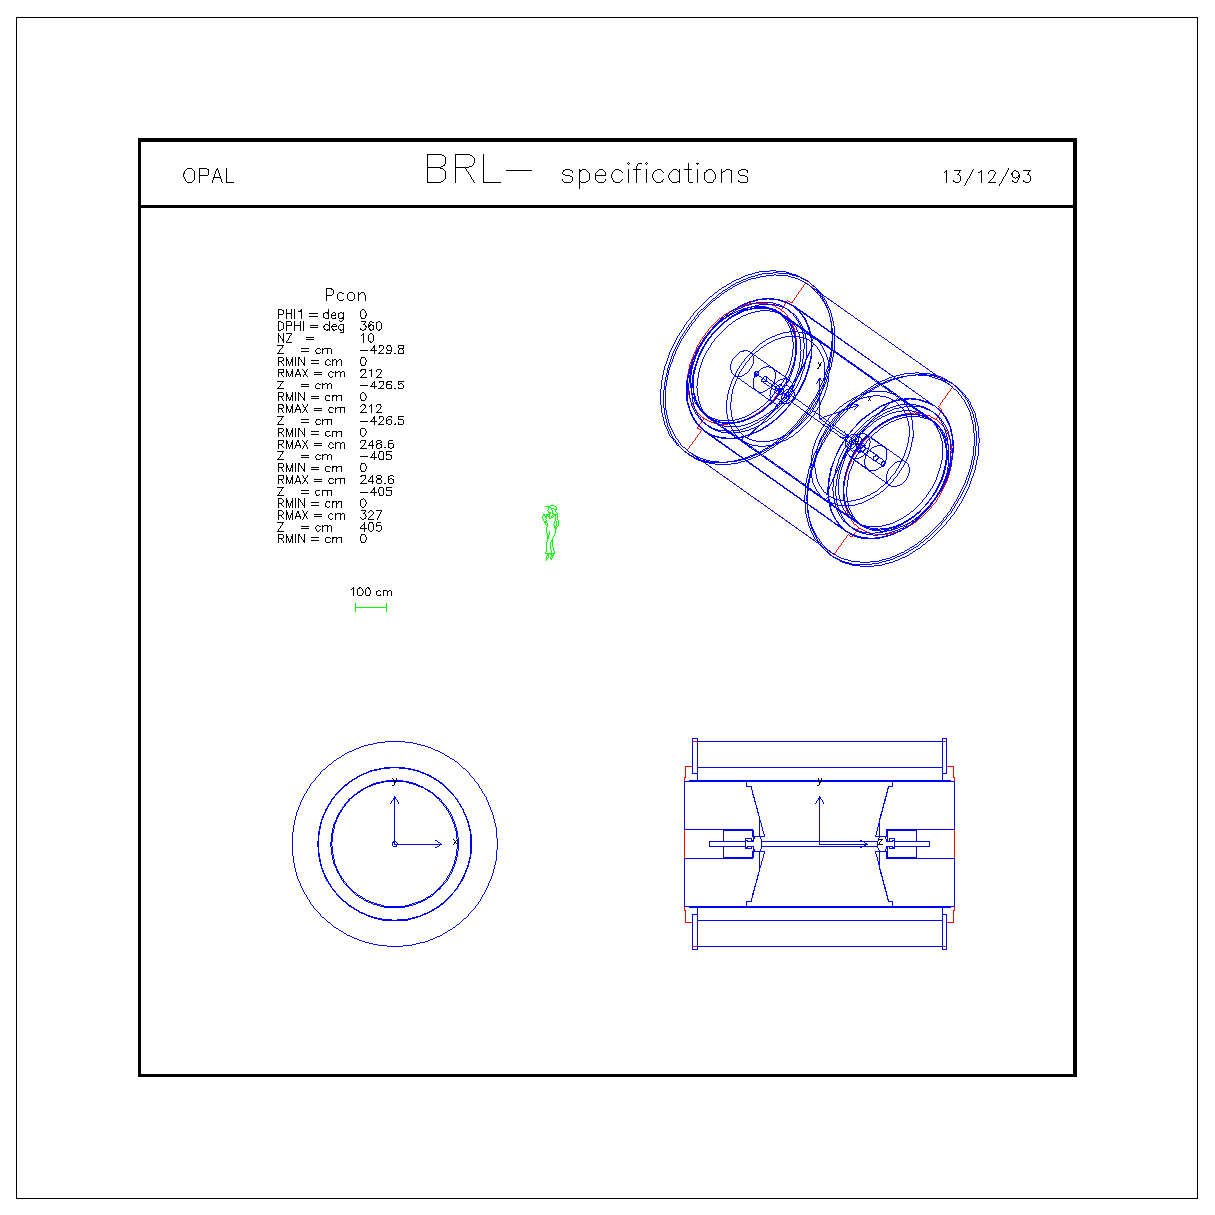
\epsfig{file=eps/draw220-1.eps,width=14cm}
     \caption{Example of use of {\tt GDSPEC}}
     \label{fg:draw220-1}
\end{figure}

The following information on the volume are
presented in a single frame:
\begin{itemize}
\item the volume daughters (one level down in the geometrical tree);
\item a space view of the volume (with $\theta$=45 and $\phi$=135);
\item a front view cut; 
\item a side view cut; 
\item the axes of the local coordinate system;
\item a human figure;
\item the scale;
\item the shape type;
\item all the numerical parameters that define the volume.
\end{itemize}
In drawing the volumes \Rind{GDSPEC} turns on the sets visibility 
({\tt 'SEEN'}) attribute for the volume {\tt CHNAME}
itself and its direct descendents. The setting of drawing options
({\tt HIDE}, {\tt CVOL}, {\tt FILL} $\ldots$) will be respected, allowing to 
customise the drawing. An example is shown in Fig.~\ref{fg:draw220-2}.
 
\begin{figure}[hbt]
     \centering
     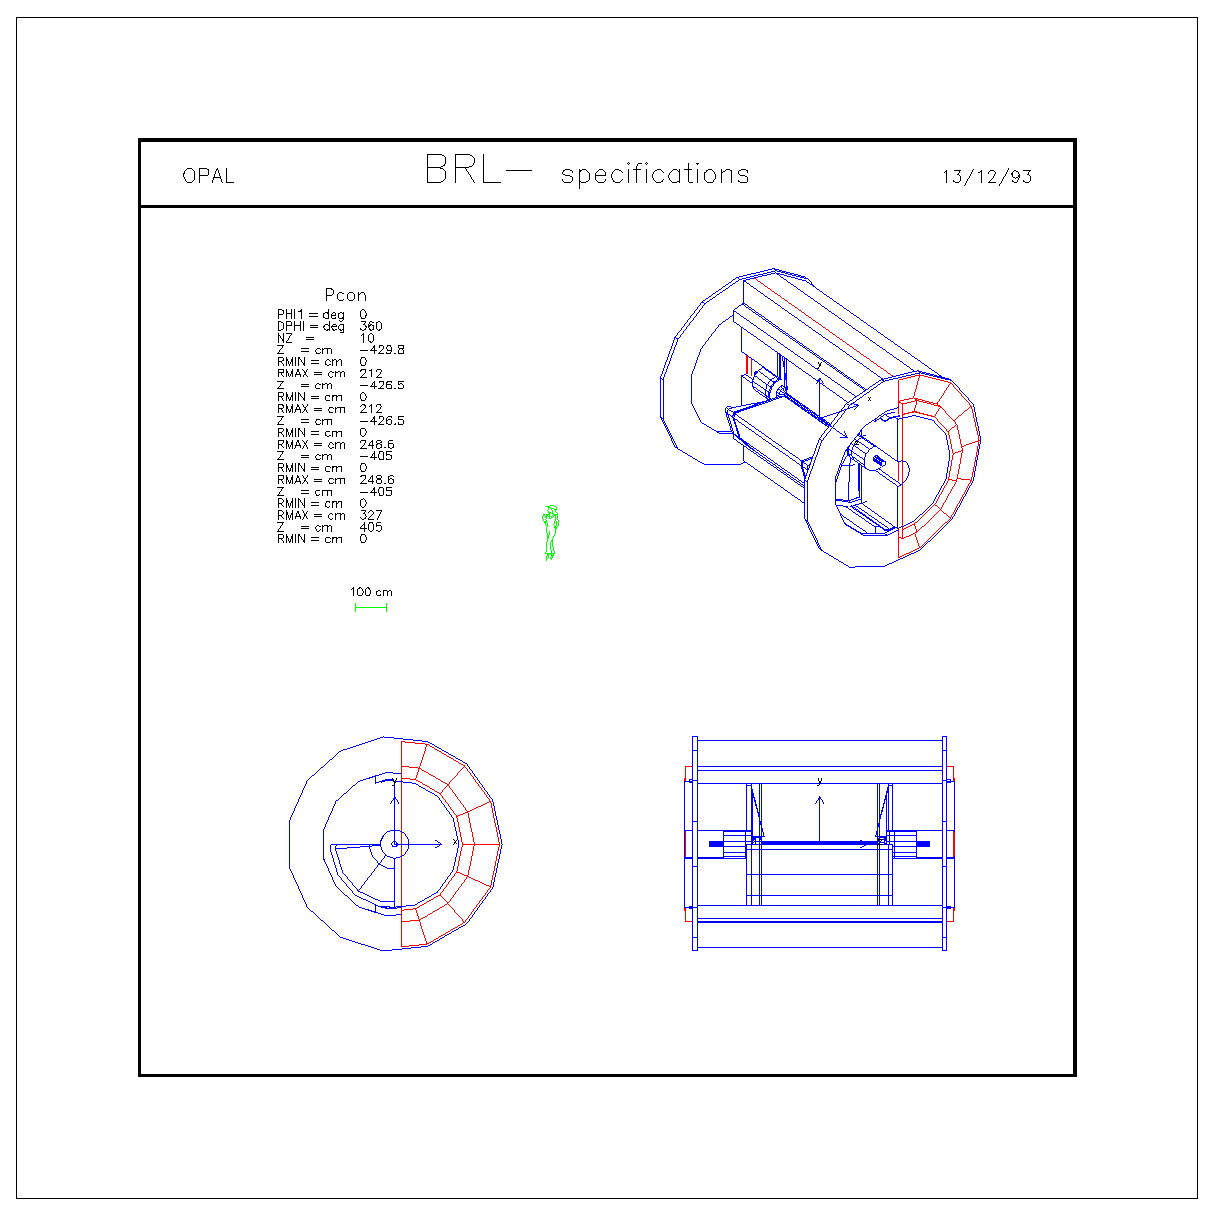
\epsfig{file=eps/draw220-2.eps,width=14cm}
     \caption{Example of use of {\tt GDSPEC}}
     \label{fg:draw220-2}
\end{figure}

\Shubr{GDFSPC}{(CHNAME,ISORT,INTER)}
Draws on separate pictures the full set of \Rind{GDSPEC} for the geometrical
tree starting from {\tt CHNAME}, i.e. calls \Rind{GDSPEC} for
the volume {\tt CHNAME} and for all its descendants.
\begin{DLtt}{MMMMMMMM}
\item[CHNAME] ({\tt CHARACTER*4}) volume name;
\item[ISORT] ({\tt INTEGER}) alphabetic sorting flag;
\begin{DLtt}{MMMM}
\item[$= 1$] all the volumes will be drawn in ascending alphabetic order
according to their name;
\item[$\neq 1$] the volumes will be drawn in the order in which they
have been created;
\end{DLtt}
\item[INTER] ({\tt INTEGER}) interactive/batch version flag;
\begin{DLtt}{MMMM}
\item[$= 1$] the routine will prompt the user at each plot
before doing a clear screen;
\item[$\neq 0$] the routine will clear automatically the screen 
before starting a new frame.
\end{DLtt}

{\bf Note:} {\tt INTER} should be set to 1 when using the interactive version 
of {\tt GEANT} and to any other value when using a batch version.
\end{DLtt}

%%%%%%%%%%%%%%%%%%%%%%%%%%%%%%%%%%%%%%%%%%%%%%%%%%%%%%%%%%%%%%%%%%%
%                                                                 %
%  GEANT manual in LaTeX form                              %
%                                                                 %
%  Michel Goossens (for translation into LaTeX)                   %
%  Version 1.00                                                   %
%  Last Mod. Jan 24 1991  1300   MG + IB                          %
%                                                                 %
%%%%%%%%%%%%%%%%%%%%%%%%%%%%%%%%%%%%%%%%%%%%%%%%%%%%%%%%%%%%%%%%%%%
\Origin{R.Brun, P.Zanarini}
\Revision{S.Giani}
\Documentation{P.Zanarini, S.Giani, F.Carminati}                   
\Submitted {01.10.83}                   \Revised{13.12.93}
\Version{Geant 3.16}                    \Routid{DRAW300}
\Makehead{Handling View banks}
\section{The view banks}
The basic detector drawing routines (\Rind{GDRAW}, \Rind{GDRAWC}, 
\Rind{GDRAWX}) scan the data structure {\tt JVOLUM} repeatedly to
extract position and dimension information on the volumes. This can
be a rather lengthy process even on fast computer. 
Hidden line removal drawing requires
an auxiliary data structure and the 
relative visibility of all the volumes has to be analysed. With complicated 
detectors the time spent in this process can be substantial, depending 
on the drawing options chosen and on the speed of the machine on which 
the program is run. In order to alleviate this problem the graphic
{\it banks} and the associated routines have been developed.

The interpretation
of the structure (for instance scanning of the volumes' data structure 
to convert the 3D geometry structure into a set 
of 2D lines, visibility analysis, surface creation or
light processing) is thus separate
from the drawing itself. In this way, the interpretation is performed 
only once and all the 2D information is stored in view banks (data 
structure {\tt JDRAW} {\tt [DRAW399]}). These views can then be displayed
quickly, having only to draw the 2D vectors or the fill
areas previously stored. 

For a detector with more than 100 different volumes, for example, 
this costs only a few thousand words of memory for 
each drawing stored.

If the drawing routines are called while a view bank, identified by
a positive integer, is open (\Rind{GDOPEN})
only interpretation will be made,
no output will be generated until the bank is closed (\Rind{GDCLOS}).
When a view bank has been closed it cannot be modified, but
it can be displayed as many times as wanted (\Rind{GDSHOW}) or deleted
(\Rind{GDELET}).

Once a drawing (detectors, tracks or hits) is in a view bank, it is 
possible to scan it in detail via the {\tt LENS} or {\tt ZOOM} interactive
commands (only available with {\tt X11}). For more information see
the {\tt [XINT]} section.

\Shubr{GDOPEN}{(IVIEW)}

\begin{DLtt}{MMMMMMMM}
\item[IVIEW] ({\tt INTEGER}) view bank number ({\tt IVIEW>0}).
\end{DLtt}

Opens a {\it view bank}, used to store 2D graphics information
coming from the interpretation of 3D structures (but also 2D annotation).
All subsequent calls to the drawing routines will fill the
view bank {\tt IVIEW}, without generating any output.
\Shubr{GDCLOS}{}
Closes the current opened view bank. Once a view bank has been closed
no more drawing can be added to it. A call to \Rind{GDCLOS} also restores the
screen.

\Shubr{GDSHOW}{(IVIEW)}

\begin{DLtt}{MMMMMMMM}
\item[IVIEW] ({\tt INTEGER}) view bank number ({\tt IVIEW>0}).
\end{DLtt}

Displays view bank {\tt IVIEW}. \Rind{GDSHOW} can be called either
before or after a view bank has been closed. If a view bank is currently
open, the content of bank {\tt IVIEW} will be added to it.

\begin{figure}[hbt]
     \centering
     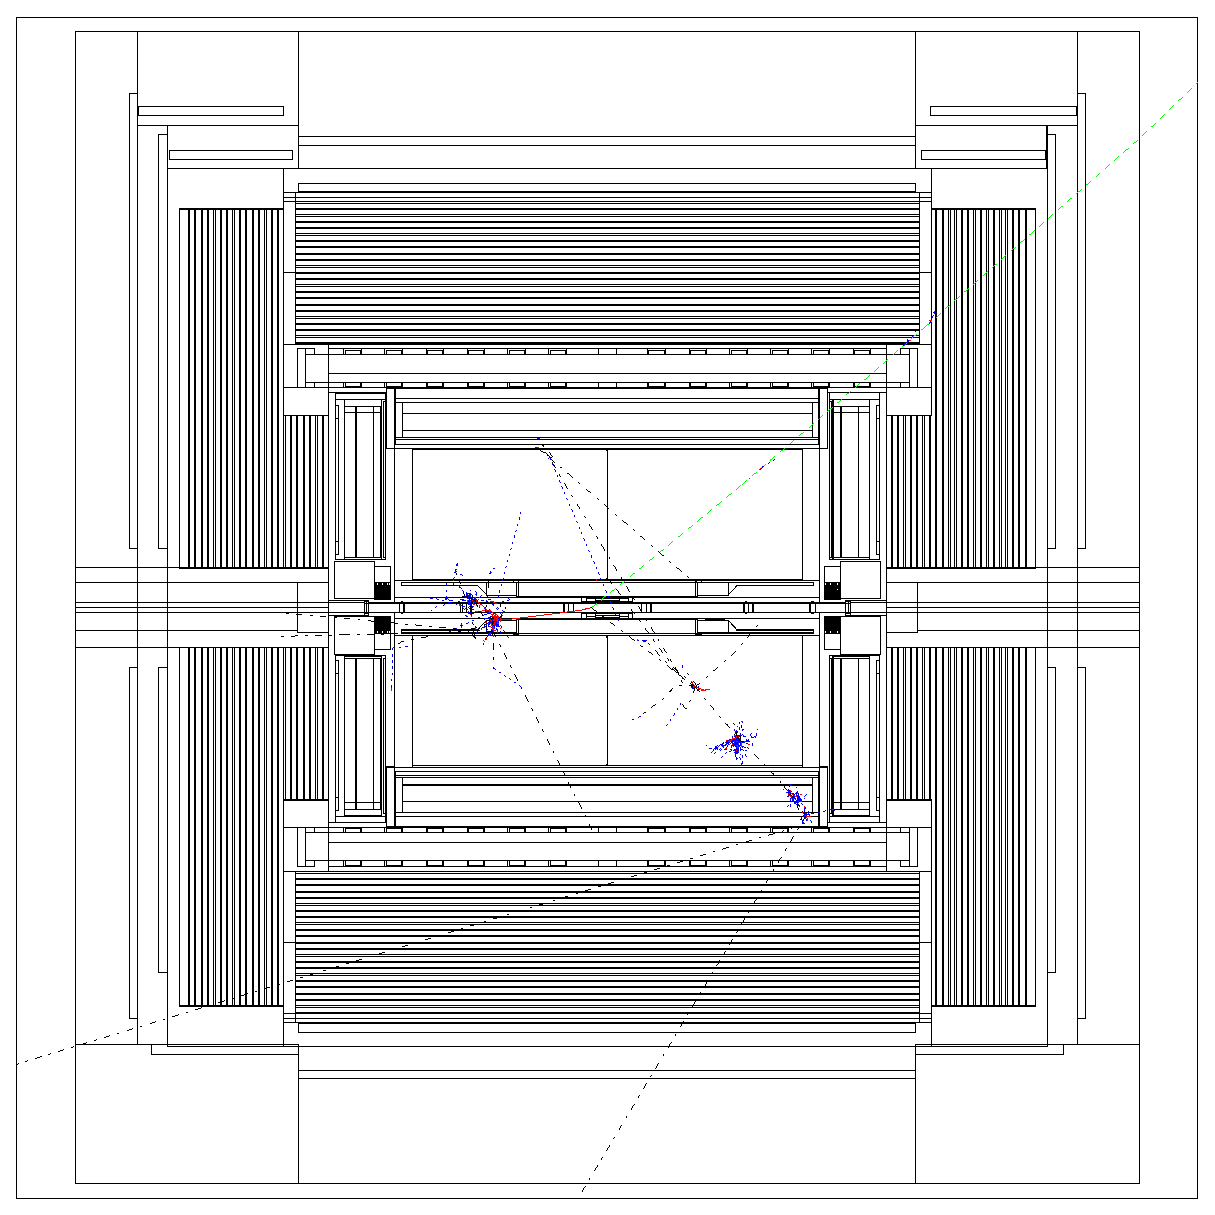
\epsfig{file=eps/draw300-1.eps,width=12.cm}
\begin{verbatim}
      CALL GDOPEN(3)
      CALL GDRAWC('ALEF',2,5.,10.,10.,0.013,0.013)
      CALL GDCLOS
      CALL GDSHOW(3)
      .
      .
      CALL GDXYZ(0)
\end{verbatim}
     \caption{Example of use of view banks}
     \label{fg:draw300-1}
\end{figure}
 
\Shubr{GDELET}{(IVIEW)}

\begin{DLtt}{MMMMMMMM}
\item[IVIEW] ({\tt INTEGER}) view bank number ({\tt IVIEW>0}).
\end{DLtt}

Deletes a view bank from memory. If called before a bank has been closed,
\Rind{GDELET} will also restore the screen mode. 

{\bf Note:} the {\tt JDRAW} data structure has a top level bank which 
contains one word for each view bank in {\tt Q(JDRAW+IVIEW)}. This
word is a key which determines the status of the bank. If this key 
is 3, the bank itself is protected against deletion, and it cannot be 
deleted by \Rind{GDELET}. An example of use of view banks is shown in 
Fig.~\ref{fg:draw300-1}.

%%%%%%%%%%%%%%%%%%%%%%%%%%%%%%%%%%%%%%%%%%%%%%%%%%%%%%%%%%%%%%%%%%%
%                                                                 %
%  GEANT manual in LaTeX form                              %
%                                                                 %
%  Michel Goossens (for translation into LaTeX)                   %
%  Version 1.00                                                   %
%  Last Mod. Jan 24 1991  1300   MG + IB                          %
%                                                                 %
%%%%%%%%%%%%%%%%%%%%%%%%%%%%%%%%%%%%%%%%%%%%%%%%%%%%%%%%%%%%%%%%%%%
\Origin{R.Brun, P.Zanarini}
\Submitted{15.11 83}     \Revised{13.12.93}
\Version{Geant 3.16}\Routid{DRAW399}
\Makehead{The data structure JDRAW}

This data structure contains the so-called \emph{view banks}. The
layout of the data structure can be found in Fig.~\ref{fg:draw399-1}.
The meaning of the variables is the following:
 
\begin{DLtt}{MMMMMMMM}
\item[NKVIEW]    number of views stored in the structure;
\item[IVIEW]     current view selected;
\item[IGU]       current graphic unit pointer;
\item[MAXGU]     number of units in graphic unit bank;
\item[MORGU]     number of words to push the graphic unit bank;
\item[IGS]       current graphic segment pointer;
\item[MAXGS]     number of segments in graphic segment bank;
\item[MORGS]     number of words to push the graphic segment bank;
\item[ITU]       current text unit pointer;
\item[MAXTU]     number of units in text unit bank;
\item[MORTU]     number of words to push the text unit bank;
\item[ITS]       current text segment pointer;
\item[MAXTS]     number of segments in text segment bank;
\item[MORTS]     number of words to push in text segment bank
\item[LENGU]     array of lengths for each graphic unit and of line attributes
({\tt LINATT});
\item[ADDGU]     array of addresses for each graphic unit;
\item[ADDTU]     array of addresses for each text unit;
\item[X]         array of u coordinates of graphic segments;
\item[Y]         array  v  coordinates of graphic segments;
\item[ICUT]      cut axis (1, 2, 3 or 0 if no cut) of the view;
\item[LINWID]    text line width and text attributes ({\tt ITXATT});
\end{DLtt}
{\tt GTHETA, GPHI, GPSI, GU0, GV0, GSCU, GSCV,} are the viewing
parameters stored in \FCind{/GCDRAW/}.
 
{\tt U0, V0, SIZE, ANGLE, IOPT, ITEXT} have the same meaning
of those given as arguments to \Rind{GDRAWT} (or \Rind{HPLSOF}~\cite{bib-HPLOT}).
 
A control word is stored in {\tt Q(JDRAW+IVIEW)}, with the following
meaning:
\begin{DLtt}{MMMM}
\item[1]  empty bank (created by internal routines to avoid gaps) or
for deleted banks;
\item[2]  bank created by the user;
\item[3]  protected bank reserved for internal use: it cannot be deleted by 
the user.
\end{DLtt}
\begin{figure}[hbt]
     \centering
     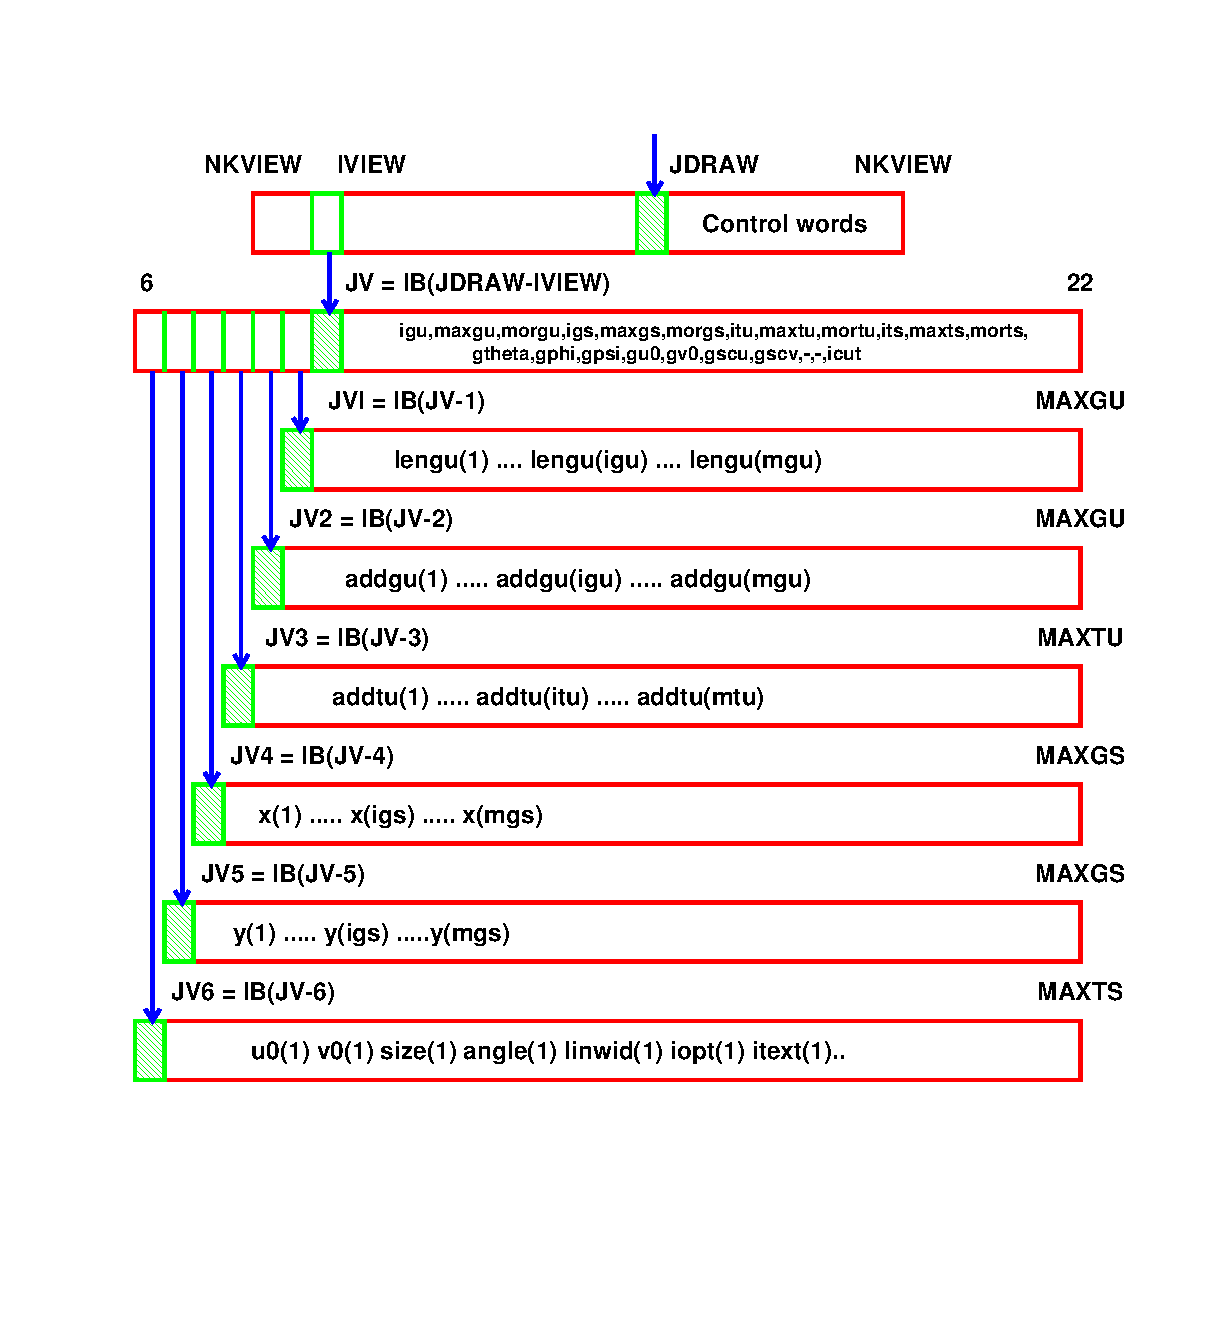
\epsfig{file=eps/draw399-1.eps,width=14cm}
     \caption{The {\tt JDRAW} data structure}
     \label{fg:draw399-1}
\end{figure}

%%%%%%%%%%%%%%%%%%%%%%%%%%%%%%%%%%%%%%%%%%%%%%%%%%%%%%%%%%%%%%%%%%%
%                                                                 %
%  GEANT manual in LaTeX form                                     %
%                                                                 %
%  Michel Goossens (for translation into LaTeX)                   %
%  Version 1.00                                                   %
%  Last Mod. Jan 24 1991  1300   MG + IB                          %
%                                                                 %
%%%%%%%%%%%%%%%%%%%%%%%%%%%%%%%%%%%%%%%%%%%%%%%%%%%%%%%%%%%%%%%%%%%
\Origin{P.Zanarini}
\Revision{S.Giani}
\Documentation{P.Zanarini, S.Giani, F. Carminati}
\Submitted {15.08.83}          \Revised{16.12.93}
\Version{Geant 3.16}\Routid{DRAW400}
\Makehead{Utility routines of the drawing package}


\Shubr{GDOPT}{(CHOPT,CHVAL)}
 
\begin{DLtt}{MMMMMMMM}
\item[CHOPT] ({\tt CHARACTER*4}) option to be set;
\item[CHVAL] ({\tt CHARACTER*4}) value to be assigned to the option.
\end{DLtt}

Drawing options can be set via the routine \Rind{GDOPT} 
(corresponding to the {\tt DOPT} interactive command).
The possible value of {\tt CHOPT} and of {\tt CHVAL} are the following:
\begin{DLtt}{MMMMMMMM}
\item[PROJ] selects the type of projection, it can have the following
values:
\begin{DLtt}{MMMMMM}
\item[PARA] orthographic parallel projection (the default);
\item[PERS] perspective projection.
\end{DLtt}
\item[THRZ] acronym for {\tt T}racks and {\tt H}its in a {\tt R}adius 
versus {\tt Z} projection, where {\tt R} is the {\it vertical} axis
of the drawing and
{\tt Z} the horizontal one. If a {\it cut view} has been drawn with the
following parameters:
\begin{DLtt}{MMMMMMM}
\item[X-Z cut] {\tt CUTTHE=90} and {\tt CUTPHI=90} in \Rind{GDRAWX} or
{\tt icut=2} in \Rind{GDRAWC};
\item[Y-Z cut] {\tt CUTTHE=90} and {\tt CUTPHI=180} in \Rind{GDRAWX} or
{\tt icut=1} in \Rind{GDRAWC}.
\end{DLtt}
the different values of the option {\tt THRZ} have the following effect
on the drawing of hits and tracks:
\begin{DLtt}{MMMMMM}
\item[360] hits and tracks will be rotated around {\tt Z} onto the
{\tt Z-R, R$>$0} half plane;
\item[180] (equivalent to {\tt ON}) hits and tracks will be rotated
around {\tt Z} onto the {\tt Z-R} plane by the smaller $\phi$ angle,
so to conserve the sign of their {\tt R}-ordinate (where {\tt R} is
either {\tt X} or {\tt Y};
\item[OFF] (the default) tracks and hits will be projected from their
position in space onto the plane {\tt R-Z}.
\end{DLtt}
 
{\bf Note:} when the {\tt THRZ} option is set to {\tt ON} or {\tt 180},
particles originating in one half space and crossing the horizontal axis
will be reflected back into the original half space. If the option 
{\tt 360} can be 
chosen, all tracks and hits are on the top (positive) half space.
\item[TRAK] selects the way tracks are drawn. Possible values:
\begin{DLtt}{MMMMMM}
\item[LINE] (the default) the lines joining track points are drawn by 
{\tt GDXYZ};
\item[POIN] only the track points are drawn.
\end{DLtt}
\item[HIDE] selects the hidden line removal technique for the
drawings. Possible values are:
\begin{DLtt}{MMMMMM}
\item[OFF] (the default) hidden lines are not removed from the drawing:
the drawing is usually rather fast, but the result can be
quite messy if a large number of volumes is visible;
\item[ON] hidden lines are not drawn: if this value is selected, the 
detector can be exploded (interactive command {\tt BOMB}), cut with 
different shapes (interactive command menu {\tt CVOL}), and some parts 
can be shifted from their original position (interactive command 
{\tt SHIFT}). Drawing with hidden line removal can be demanding in
terms of CPU time and memory. At the end of each drawing
the program displays the memory used and the statistics on the 
volume visibility. When the drawing requires more memory 
than available, the program will evaluate and display the number of 
missing words, so that the user can increase accordingly the
size of the \Rind{ZEBRA} store in the common \FCind{/GCBANK/}.
\end{DLtt}
\item[SHAD] when {\tt HIDE} is {\tt ON}, selects the 
shading and filling option for the detector's surfaces that are drawn:
\begin{DLtt}{MMMMMM}
\item[OFF] (the default) no shading of the surfaces will be performed;
\item[ON]  the volume surfaces will be filled according to the value of 
their {\tt FILL} and {\tt LWID} attribute, set via {\tt GSATT}:
\begin{DLtt}{MMMMMM}
\item[FILL$=$1] the surfaces are filled with the current colour assigned
to the volume via \Rind{GSATT}, 166 different colours are available;
\item[FILL$>$1] the surfaces are filled with a shade of the basic colour
assigned to the volume according to their angle with respect to the line
of illumination, the resolution
increases with the value of {\tt FILL} (1$<$ {\tt FILL} $\leq$ 7);
\item[LWID$>$0] just as the number of scan-lines used to fill a surface
depends on the value of {\tt FILL}, their width depends on the value of 
{\tt LWID}: increasing the value of {\tt LWID} will result in thicker lines.
\end{DLtt}
\end{DLtt}
\item[EDGE] control drawing of the volume edges in {\tt HIDE=ON, FILL=ON}
mode:
\begin{DLtt}{MMMMMM}
\item[ON] the edges of the faces are not drawn,
so that they will be visible only as intersections of filled faces
with different luminosity; 
\item[OFF] the edges of the faces are drawn.
For the volumes which are not filled, the normal
edges will be drawn irrespective of the value of this option.
\end{DLtt}
\end{DLtt}

\Shubr{GDZOOM}{(ZFU,ZFV,UZ0,VZ0,U0,V0)}
\begin{DLtt}{MMMMMMMM}
\item[ZFU]    ({\tt REAL}) zoom factor for {\tt U} coordinate;
\item[ZFV]    ({\tt REAL}) zoom factor for {\tt V} coordinate;
\item[UZ0]    ({\tt REAL}) {\tt U} coordinate of centre of zoom;
\item[VZ0]    ({\tt REAL}) {\tt V} coordinate of centre of zoom;
\item[U0]     ({\tt REAL}) {\tt U} coordinate of centre of zoom 
in the resulting picture;
\item[V0]     ({\tt REAL}) {\tt V} coordinate of centre of zoom 
in the resulting picture.
\end{DLtt}
This routine sets the zoom parameters (part of the viewing parameters 
in common \FCind{/GCDRAW/}) that define how objects 
will be displayed by the subsequent drawing operations.
The zoom is computed around {\tt UZ0}, {\tt VZ0} (user coordinates).
This point will be moved to {\tt U0}, {\tt V0} in the resulting picture.
{\tt ZFU}, {\tt ZFV} are the zoom factors (positive). If {\tt ZFU} 
or {\tt ZFV} are zero, the zoom parameters are reset, and the 
original viewing is restored.

\Shubr{GDAXIS}{(X0,Y0,Z0,AXSIZ)}
\begin{DLtt}{MMMMMMMM}
\item[X0]    ({\tt REAL}) {\tt X} coordinate of origin;
\item[Y0]    ({\tt REAL}) {\tt Y} coordinate of origin;
\item[Z0]    ({\tt REAL}) {\tt Z} coordinate of origin;
\item[AXSIZ] ({\tt REAL}) axis size in centimeters.
\end{DLtt}
Draws the axes of the {\tt MA}ster {\tt R}eference {\tt S}ystem,
corresponding to the current viewing parameters.
All the arguments refer to the {\tt MARS}.

\Shubr{GDSCAL}{(U0,V0)}
\begin{DLtt}{MMMMMMMM}
\item[U0]    ({\tt REAL}) {\tt U} coordinate of the centre of the scale;
\item[V0]    ({\tt REAL}) {\tt V} coordinate of the centre of the scale.
\end{DLtt}
Draws a scale corresponding to the current viewing parameters.
Seven kinds of units are available, from 1 micron to 100 cm.
The best unit is automatically selected.

\Shubr{GDMAN}{(U0,V0)}
\Shubr{GWOMA1}{(U0,V0)}
\Shubr{GDWMN2}{(U0,V0)}
\Shubr{GDWMN3}{(U0,V0)}
\begin{DLtt}{MMMMMMMM}
\item[U0]     ({\tt REAL}) {\tt U} coordinate of the centre of the figure;
\item[V0]     ({\tt REAL}) {\tt V} coordinate of the centre of the figure.
\end{DLtt}
Draws the profile of a man, or three different female figures
in 2D user coordinates, with the current scale factors.
The figure is approximately 160 cm high.

\Shubr{GDRAWT}{(U,V,CHTEXT,SIZE,ANGLE,LWIDTH,IOPT)}
\begin{DLtt} {MMMMMMMM}
\item[U]    ({\tt REAL}) {\tt U} position of text string;
\item[V]   ({\tt REAL}) {\tt V}   position of text string;
\item[CHTEXT] ({\tt CHARACTER*(*)}) text string;
\item[SIZE]   ({\tt REAL}) character size (cm);
\item[ANGLE]  ({\tt REAL}) rotation angle (degrees);
\item[LWIRTH] ({\tt INTEGER}) line width (1,2,3,4,5);
\item[IOPT]  ({\tt INTEGER}) centering option for the text:
\begin{DLtt}{MMMM}
\item[-1] left adjusted;
\item[~0] centered;
\item[~1] right adjusted.
\end{DLtt}
\end{DLtt}
Draws text with software characters. It has the same
arguments of the {\tt HPLOT}\cite{bib-HPLOT} routine \Rind{HPLSOF} 
(a call to \Rind{HPLSOF} is actually performed).

\Shubr{GDRAWV}{(U,V,NP)}
\begin{DLtt}{MMMMMMMM}
\item[U]    ({\tt REAL}) array of {\tt U} coordinates;
\item[DT]   ({\tt REAL}) array of {\tt V} coordinates;
\item[NP]   ({\tt INTEGER}) number of points.
\end{DLtt}
Draws 2D polylines in user coordinates.
The routine \Rind{GDFR3D} can be called to transform 3D points 
in 2D user coordinates.

\Shubr{GDHEAD}{(ISEL,CHNAME,CHRSIZ)}
\begin{DLtt}{MMMMMMMM}
\item[ISEL]  ({\tt INTEGER}) option to be selected for the title name 
(decimal integer):
\begin{DLtt}{MMMMMMM}
\item[~~~~~0] only the header lines;
\item[xxxxx1] add the text {\tt CHNAME} centered on top of header;
\item[xxxx1x] add global detector name (first volume) on left;
\item[xxx1xx] add date on right;
\item[xx1xxx] select thick characters for text in top of head (i.e. 
with larger line width);
\item[x1xxxx] add the text {\tt EVENT NR x} on top of header;
\item[1xxxxx] add the text {\tt RUN NR x} on top of header.
\end{DLtt}

{\bf Note:} {\tt ISEL=x1xxx1} or {\tt ISEL=1xxxx1} are illegal choices,
i.e. they generate overwritten text.
\item[CHNAME] ({\tt CHARACTER*4}) title string;
\item[CHRSIZ] ({\tt REAL}) character size (cm) of text {\tt CHNAME}.
\end{DLtt}
This routine draws a frame header.

\Shubr{GDCOL}{(ICOL)}

{\bf This routine has been kept for backward compatibility. The appropriate
{\tt HIGZ} routines should be called instead.}

\begin{DLtt}{MMMMMMMM}
\item[ICOL] ({\tt INTEGER}) colour code (1,2,\ldots,8), 
it can be positive, negative, 
or zero:
\begin{DLtt}{MMMM}
\item[$>$0] to set the colour permanently;
\item[$<$0] to set the colour temporarily;
\item[$=$0] to restore the permanent colour value.
\end{DLtt}
\end{DLtt}
This routine sets the colour code.
For example we can set {\tt ICOL=-1} to start with colour  1,
then change to {\tt ICOL=3} to set colour  3, and at the end
restore the original colour by setting {\tt ICOL=0} that
takes colour  1 again.

\Shubr{GDLW}{(LW)}

{\bf This routine has been kept for backward compatibility. The appropriate
{\tt HIGZ} routines should be called instead.}

\begin{DLtt}{MMMMMMMM}
\item[ LW] ({\tt INTEGER}) line width code (1,2,\ldots,5), it can be positive, 
negative, or zero:
\begin{DLtt}{MMMM}
\item[$>$0] to set the line width permanently;
\item[$<$0] to set the line width temporarily;
\item[$=$0] to restore the permanent line width value.
\end{DLtt}
\end{DLtt}
This routine sets the line width.
For example we can set {\tt LW=-1} to start with line width  1,
then change to {\tt LW=3} to set line width 3, and at the end
restore the original line width by setting {\tt LW=0} that
takes line width  1 again.

\Shubr{GDCURS}{(U0*,V0*,ICHAR*)}
\begin{DLtt}{MMMMMMMM}
\item[U0]   ({\tt REAL}) {\tt U} coordinate of the graphics cursor;
\item[V0]   ({\tt REAL}) {\tt V} coordinate of the graphics cursor;
\item[ICHAR] ({\tt INTEGER}) {\tt ASCII} value of the key pressed.
\end{DLtt}
A graphics input is provided by this routine to fetch the 2D user coordinates
of the graphics cursor on the screen.
Interactive commands to zoom, 
measure, or pick tracks or hits make use of this routine.
When the routine is called in the interactive
version of {\tt GEANT},
the present position of the graphics cursor on the screen becomes visible and
it can be moved with the mouse. The user then positions the 
cursor and presses the left button. 
The routine returns then in {\tt U0}, {\tt V0} the user coordinates
of the graphics cursor.
On terminals which do not have the mouse, the graphic cursor is moved
with the arrows, and the point is acquired when any key, except {\it carriage
return}, is pressed. In this case the routine returns in {\tt ICHAR} the 
{\tt ASCII} value of the key pressed. If the user types the carriage return, 
the previous value is retained.

\Shubr{GDFR3D}{(X,NPOINT,U*,V*)}
\begin{DLtt}{MMMMMMMM}
\item[X]      ({\tt REAL}) array {\tt X(3,NPOINT)} of space points;
\item[NPOINT] ({\tt INTEGER}) number of points:
\begin{DLtt}{MMMM}
\item[$>$0] {\tt X} is in the current {\tt DRS};
\item[$<$0] {\tt X} is in {\tt MARS};
\end{DLtt}
\item[U]  ({\tt REAL}) array of {\tt NPOINT U} coordinates;
\item[V]  {(\tt REAL}) array of {\tt NPOINT V} coordinates.
\end{DLtt}
Converts from 3D space coordinates (either in {\tt MA}ster or 
{\tt D}aughter {\tt R}eference {\tt S}ystem) to the corresponding 2D 
user coordinates.
 
This routine maps a space point ({\tt X, Y, Z} in a right-handed reference 
system) onto a plane perpendicular to the observer's line of sight,
defined by the spherical angles $\theta$, $\phi$:
\begin{DLtt}{MMMM}
\item[${\tt \theta}$] the angle between the line of sight and the {\tt Z} 
axis ($0 \leq \theta \leq 180$);
\item[${\tt \phi}$] the angle between the {\tt X} axis and the projection 
onto the {\tt X-Y} plane of the line of sight ($0 \leq \phi \leq 360$).
\end{DLtt}
The plane onto which the point is mapped is actually the {\tt X-Y} plane 
of the {\tt P}rojection {\tt R}eference {\tt S}ystem, and
the observer's line of sight is the {\tt Z} axis of {\tt PRS}. The vertical 
axis on
this plane ({\tt Y} axis on {\tt PRS}) is obtained by intersecting this plane
with the one of {\tt MARS} or {\tt DRS} containing the line of sight and 
the {\tt Y} axis.

\Shubr{GD3D3D}{(XIN,NPOINT,XOUT*)}
\begin{DLtt}{MMMMMMMM}
\item[XIN]   ({\tt REAL}) array {\tt XIN(3,NPOINT)} of input points in 
{\tt MARS};
\item[NPOINT] ({\tt INTEGER}) number of points;
\item[XOUT]   ({\tt REAL}) array {\tt XOUT(3,NPOINT)} of output points 
in {\tt PRS}.
\end{DLtt}
Converts from 3D space coordinates in {\tt MARS}
to 3D coordinates in {\tt P}rojection {\tt R}eference 
{\tt S}ystem (whose {\tt Z} axis is along
the line of sight given by $\theta$ and $\phi$ angles).

\putbib[cnasbibl,geabibl]
\end{bibunit}
 
%%     GEOM part     %%
 
\begin{bibunit}[unsrt]
\renewcommand{\bibname}{GEOM Bibliography}
%%%%%%%%%%%%%%%%%%%%%%%%%%%%%%%%%%%%%%%%%%%%%%%%%%%%%%%%%%%%%%%%%%%
%                                                                 %
%  GEANT manual in LaTeX form                                     %
%                                                                 %
%  Michel Goossens (for translation into LaTeX)                   %
%  Version 1.00                                                   %
%  Last Mod. Jan 24 1991  1300   MG + IB                          %
%                                                                 %
%%%%%%%%%%%%%%%%%%%%%%%%%%%%%%%%%%%%%%%%%%%%%%%%%%%%%%%%%%%%%%%%%%%
\Documentation{F.Bruyant}
\Submitted{01.10.84}      \Revised{10.03.94}
\Version{Geant 3.21}\Routid{GEOM001}
\Makehead{The geometry package}

The geometry package has two main functions:

\begin{enumerate}
\item define, during the initialisation of the program,
the geometry in which the particles will be tracked;
\item communicate, during the event processing phase, to the tracking 
routines the information for 
the transport of the particles in the geometry which has been defined.
\end{enumerate}

The present section reviews the concepts of the geometry package and explains
how the geometrical information should be provided by the user.
It is important to point out that, once the geometry has been defined,
the tracking of particles through the different volumes proceeds without any
intervention from the user {\tt [TRAK]}. 

The connection between the
geometry and tracking packages is established by the subroutines
\Rind{GMEDIA}/\Rind{GTMEDI}, \Rind{GTNEXT}/\Rind{GNEXT} and
\Rind{GINVOL} which answer respectively the questions:
\begin{itemize}
\item    In which volume is a given point ?
\item    What is the distance to the nearest volume along the trajectory
of the particle ?
\item    What is the distance to the nearest volume ?
\item    Is a given point still in the current volume ?
\end{itemize}
The routines \Rind{GTMEDI}, \Rind{GTNEXT} are used in a dynamic context,
at tracking time, when the
knowledge of the track direction can be used to save time.
\section{ The volume definition }

Experimental setups, as complex as the LEP\footnote{The Large Electron Positron
collider in operation at CERN.} detectors, can be described 
rather accurately through the definition of a set of {\it volumes}.
Each {\it volume} is given a {\it name} and is characterised by:
\begin{itemize}
\item a {\it shape} identifier, specifying one of the basic
          geometrical shapes available {\tt [GEOM050]};
\item   the {\it shape} parameters, giving the dimensions of the volume;
\item   a local reference system, with origin and axes defined
for the each shape;
\item    the physical properties, given by a set of constants describing the
homogeneous {\it material} which fills the volume ({\tt [CONS]});
\item  additional properties, known as {\it tracking medium} parameters,
which depend on the characteristics of the volume itself (the
material identifier is one of the constants) and on its geometrical and
physical environment (properties of the neighbouring volumes, magnetic field, 
etc.) {\tt [CONS, TRAK]};
\item  a set of attributes, in connection with the drawing package
and the detector response package {\tt [DRAW, HITS]}.
\end{itemize}
Until it is {\it positioned} in a given reference frame,
a volume is an entity which has no spatial relation with the other volumes.
By convention, a unique initial volume has to be defined first
which will contain
all the other volumes. The reference frame intrinsic
to this volume is considered to be the master reference frame.

There are sixteen basic shapes in {\tt GEANT}, which are described in
{\tt [GEOM050]}.

\section{Volumes with contents}
A {\it volume} can be declared to have contents and as such it becomes a 
{\it mother}
volume. The contents are {\it either} predefined volumes which are explicitly 
positioned inside the mother, {\it or} new volumes which are implicitly defined
by a division mechanism applied to the mother. Positioning a volume with given 
shape and dimensions inside a mother volume is obtained by specifying its 
translation and rotation with respect to the mother reference frame. The user 
should make sure that no volume extends beyond the boundaries of its mother.

When a volume is positioned, the user gives it a {\it number}. Multiple copies 
of the same volume can be positioned inside the same or different mothers
as long as their copy numbers differ.
The contents of the positioned volume are reproduced 
in all copies. 

Mother volumes can be divided by planes along the three axes ($ x, y, z$),
radially along $R_{xy}$, or along the spherical coordinates of a 
polar system: $R$, $\theta$ and $\phi$. The axis along which it is
possible to perform a division depend on the shape to be divided. The
general rule is that the result of the division be still a {\tt GEANT} shape.

A volume can be partially or totally divided.
The division process
generates a number of {\it cells}, which are considered as new volumes.
The cell dimensions are computed
according to the number of divisions or the step size. A cell, as any
other volume, can again be divided, or have other
volumes positioned into it. Any operation of positioning or division
performed on one cell is repeated to all the cells resulting
from the division. A volume can be {\it either} divided {\it or} have
contents, but not the two things together.

These operations define a physical tree with several
levels. The material and properties of the contents replace the
ones of the mother within the space region they occupy.
A {\tt volume} is therefore defined not only by its intrinsic characteristics
but also by those of its {\it descendants}, namely its contents (by
division or positioning), the contents of its contents, etc.

\section{ Overlapping volumes, see also {\tt [GEOM020]} }
The user may define volumes which have no relation with the real
objects. It is sometimes convenient to make use of such volumes,
to artificially delimit regions with simple shapes.
Doing this, it may happen that
volumes partially overlap each other. (A volume positioned inside a mother is
obviously not regarded as overlapping the mother).

It is possible in {\tt GEANT} to handle partially overlapping volumes, but
there are some implications that the user should be aware of.
A flag {\tt 'ONLY'/'MANY'} is assigned to each copy of a given volume at the 
moment this is positioned. The {\tt 'MANY'} option indicates that
a point found in this volume could also be in other volumes which are
not its direct descendants. If one of the
overlapping volumes where the point is found is declared as {\tt 'ONLY'}, the
geometry subroutines will give priority to this volume, 
and the search stops.
If a point is inside several {\tt 'MANY'} volumes and outside all {\tt 'ONLY'}
ones, priority will be given to the volume
found at the deepest level, or to the first found, if there are many
valid {\tt 'MANY'} candidates at the same level. In order to avoid ambiguities,
two overlapping {\tt 'MANY'} volumes should in general
have the same tracking medium.

\section{The physical tree}
An example of a 4 level physical tree with embedded volumes and
the corresponding geometrical configuration are shown in fig~\ref{fg:geom001-1}.

\begin{figure}[hbt]
      \centering
      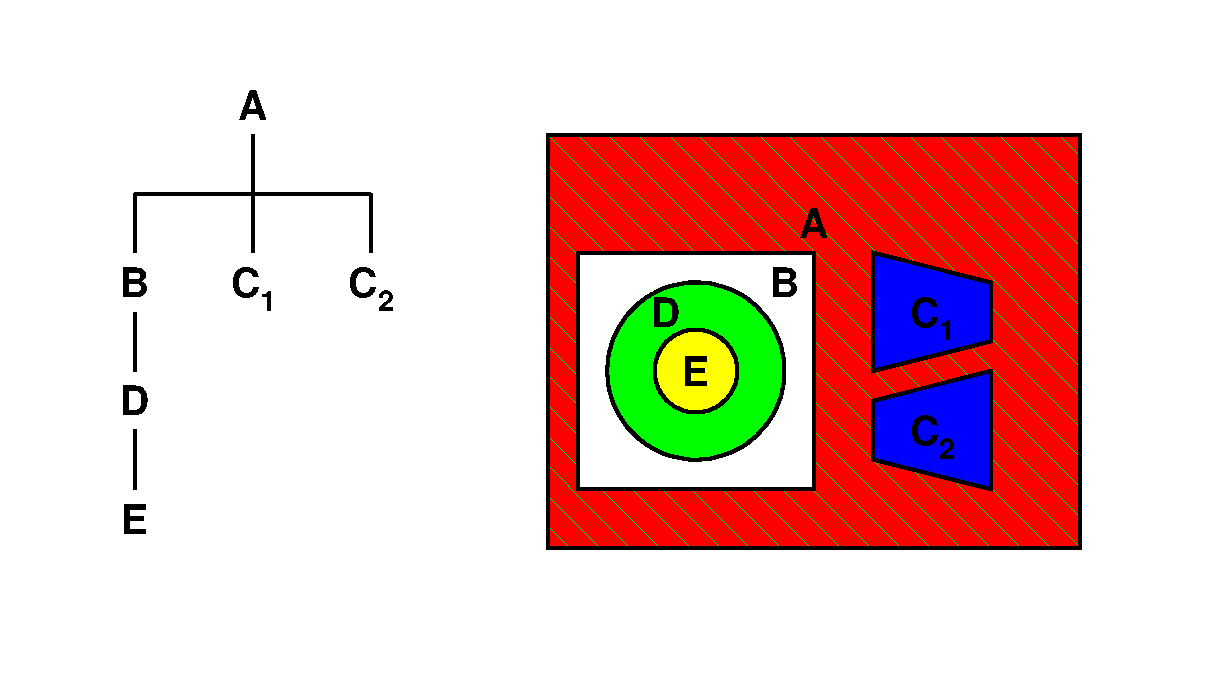
\epsfig{file=eps/geom001-1.eps,width=16cm}
      \caption{Example of geometrical tree structure}
      \label{fg:geom001-1}
\end{figure}

where A and B are {\tt BOX}es, C a {\tt TRAP}ezoid, and D and E {\tt TUBE}s
(see {\tt [GEOM050]} for more detail).
Notice that the same physical configuration could be described as well though
a 3 level tree if D were defined as a {\it hollow}
{\tt TUBE}, with inner radius non-zero and E
directly positioned into B.
The package accepts a maximum of 15 levels, which should be
enough to represent the fine details of a complex structure.
\section{The data structures {\tt JVOLUM} and {\tt JGPAR}
and the common {\tt /GCVOLU/}}

In practice, the physical tree is not represented as such in the
data part of the program. Instead, a logical tree structure is defined,
the {\tt JVOLUM} data structure, which describes the arrangement of
volumes in a compact and recurrent way. Each generic volume appears once,
and once only, and carries the information relevant to the volume itself
and to its contents, if any, by reference to the
generic volumes corresponding to those contents.
In the situation where division or multiple copies occur, there
is no longer a one-to-one correspondence between a volume in the
logical tree and a region in space. Information has to be added at
tracking time to identify which division cell or which copy was considered
at each depth level along the path through the physical tree. This
information is stored by the subroutine \Rind{GMEDIA}/\Rind{GTMEDI}, for the
current point of the current track, in the common \FCind{/GCVOLU/}. It includes
the current level number {\tt NLEVEL} and, for each level, starting from the
first mother volume, the identification of the corresponding volume, e.g.:
{\tt NAME}, {\tt NUMBER}, {\tt 'ONLY'/'MANY'} flag, translation and rotation
with respect to the master reference frame and so on. 
The number of shape parameters
and pointers to the vector describing the actual values of those
parameters, for each level, are stored in the data part and in the link
part, of the data structure {\tt JGPAR}, respectively.

\section{The user tools }

The geometry through which the particles are transported is defined by the
user via a set of calls to subroutines of the {\tt GEANT} package.

The user can define a volume through a call to the subroutine:
\begin{DLtt}{MMMMMMMM}
\item[\Rind{GSVOLU}] define ({\it instantiate}) a volume by giving a 
{\tt NAME} and the actual parameters to a shape; the position of the volume 
inside the bank {\tt JVOLUM} is returned. If any of the parameters which
express a length is negative, {\tt GEANT} will assign to this parameter
at tracking time
the maximum value allowed, without protruding out of the mother 
which contains the particle transported.

A shape can be instantiated
into a volume also without actual parameters. These will then be supplied
when positioning each copy of the volume via the \Rind{GSPOSP} routine (see
below). This allows to have many {\it similar} volumes with the same name
and shape, but different actual parameters in each copy.
\end{DLtt}

The user can position a volume through a call to either one of the following 
subroutines:

\begin{DLtt}{MMMMMMMM}
\item[\Rind{GSPOS}] position a copy of a volume inside its mother with respect 
to the mother's reference system. A a point in space, a rotation matrix
index, a copy number and the {\tt 'ONLY'/'MANY'} flag are supplied;
\item[\Rind{GSPOSP}] position a copy of a volume which has been instantiated
without actual parameters inside its mother with respect to the mother reference
system. The parameters of the copy being positioned are supplied as well.
The volumes will be identified by name and copy number as for multiple copies
of the same volume.
\end{DLtt}
The user can divide a volume through a call to either one of the following
subroutines:

\begin{DLtt}{MMMMMMM}
\item[\Rind{GSDVN}] divide a volume in a given {\it number} of cells completely
filling the mother. In this case the cell tracking medium
is assumed to be the same as for the mother. See also \Rind{GSDVN2}.
\item[\Rind{GSDVT}] divide a volume with slices of a given {\it step}.
The cell tracking medium can be different from the one of the mother.
See also \Rind{GSDVT2}.
\item[\Rind{GSDVX}] divide a volume starting from a given offset. In addition 
to {\tt STEP} and {\tt NDIV} (with at least one of them positive to be 
effectively useful), the origin of the first cell, the cell tracking medium 
and eventually the computed (maximum) number of divisions must be specified.
\end{DLtt}


\section{Geometrical information retrieval}

The parameters of a volume may depend on the physical tree which leads to
this volume. The dimensions of one of the slices of a cone divided along
{\tt Z} depends on which slice we consider. So a volume is completely
defined only if we specify the path in the tree. This is composed by the
name and copy number of the volumes containing the one we are interested
in, from the first mother.

Given this information, the routine \Rind{GLVOLU} is capable to fill the
common \FCind{/GCVOLU/}, and the structure {\tt JGPAR} with the actual
parameters of the instance chosen.

%%%%%%%%%%%%%%%%%%%%%%%%%%%%%%%%%%%%%%%%%%%%%%%%%%%%%%%%%%%%%%%%%%%
%                                                                 %
%  GEANT manual in LaTeX form                                     %
%                                                                 %
%  Michel Goossens (for translation into LaTeX)                   %
%  Version 1.00                                                   %
%  Last Mod. Jan 24 1991  1300   MG + IB                          %
%                                                                 %
%%%%%%%%%%%%%%%%%%%%%%%%%%%%%%%%%%%%%%%%%%%%%%%%%%%%%%%%%%%%%%%%%%%
\Documentation{S.Giani, S.Ravndal}
\Submitted{10.03.94}      \Revised{10.03.94}
\Version{Geant 3.21}\Routid{GEOM010}
\Makehead{Tracking inside volumes and optimisation}



The tracking of particles through the geometrical data structure is the key
functionality of {\tt GEANT}. 
At every particle's step, the program must find the
volume where the particle is ({\tt GTMEDI}) and the next boundary it will cross
({\tt GTNEXT}). This can take
about $60\%$ of the total simulation time (even for detectors described
in an optimized way); therefore, a new logic has been introduced to minimize
the time spent for the search in the geometrical tree. 

\section{ Virtual divisions}

Instead of a linear or
binary search (time spent proportional or logarithmic with the number of
volumes, respectively), a `direct access' technique has been developed to
make the time basically independent from the number of volumes. Every volume
containing other volumes is `virtually' divided in equal slices at 
initialization time via the call to {\tt GGCLOS}
(the best axis is computed automatically). 
For each slice,
a data structure is filled with a list of the volumes 
identifiers intersecting such
slice. 
Slices with identical lists are pointing to the same contents
and are collected. At 
tracking time it is immediate to find in which slice the particle is and only
its contents have to be checked. The same is true to find the next boundary to
be crossed: only if the intersection point with a content lies outside the 
current collection of slices, the next one will be checked. The algorithm
gives in average about a factor 2 in speed for the overall simulation in the
large detectors. It also minimizes the dependency of the performance
on the skill and experience of the programmer and allows a fast tracking even
in geometrical structures received from CAD systems.

\section{ Other optimisation tools}

The following facilities are kept for backward compatibility reasons.
If called by the user, these optimisation tools are called at 
initialisation time, but not used at tracking time. Instead, the
new optimisation using 'virtual divisions' is performed.
If the user wants to use the older optimisation tools, he can 
recompile {\tt GEANT} 3.21 using the {\tt PATCHY} flag {\tt +OLD}.
\begin{enumerate}
\item \Rind{GSORD}/\Rind{GGORD}

From the position of the contents inside a given volume, the
subroutine \Rind{GSORD} computes fictitious
boundaries along the specified coordinate, simulating
a division with irregular step size. A binary search technique is used
to identify within which pseudo-cell the current point is. The slow process
of computing whether the point is inside or outside the contents is therefore
limited to the few (if any) volumes overlapping with that
pseudo-cell, as sketched in fig~\ref{fg:geom001-2}.

\begin{figure}[hbt]
      \centering
      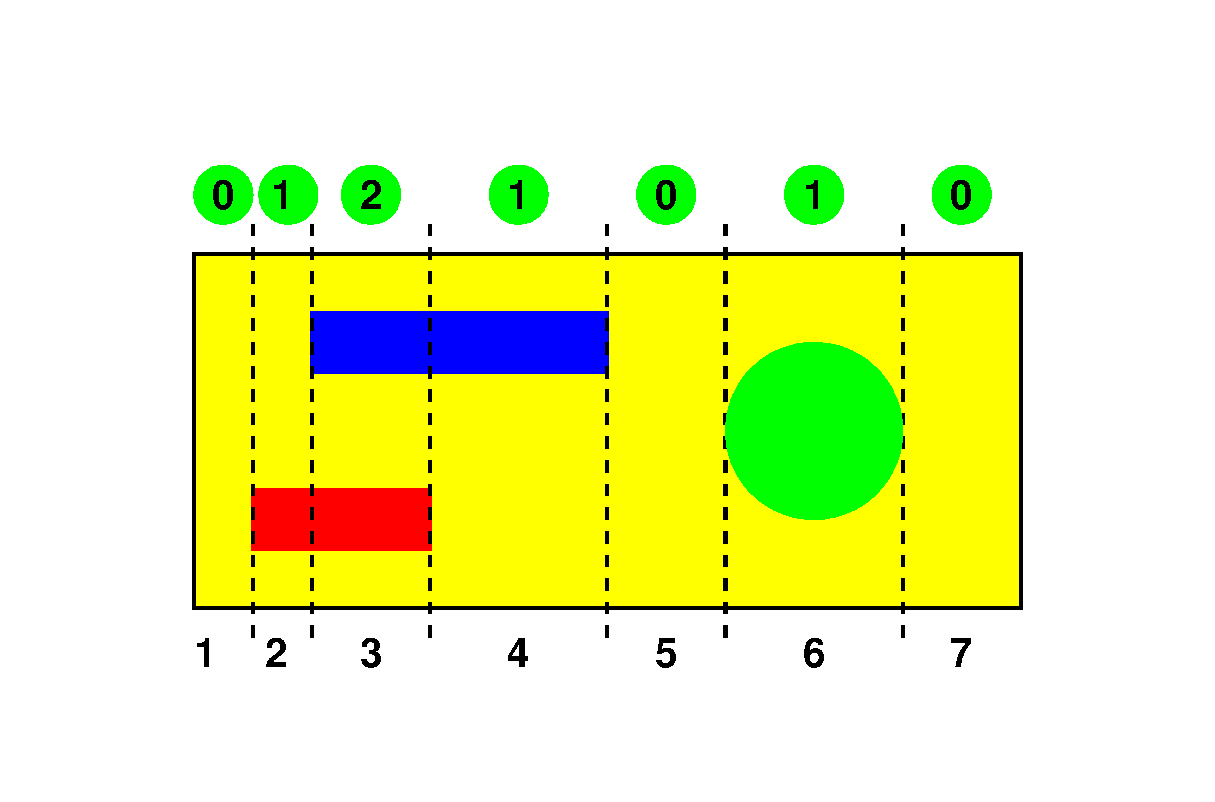
\epsfig{file=eps/geom001-2.eps,width=16cm}
      \caption{Example of pseudo-cells created by {\tt GSORD}}
      \label{fg:geom001-2}
\end{figure}

The coordinate selected for the pseudo division can be any of
{\tt X, Y, Z, $R_{xy}$, $R$, $\phi$ or $\theta$;}.
For a given volume, the call to \Rind{GSORD} has to come after all its first
level contents have been positioned.

\item
\Rind{GSNEXT}/\Rind{GSNEAR}

when a particle exits from a daugther of a 
mother volume, the contents are scanned initially
in the order in which 
they have been positioned, and the user should take care over
the best sequence of \Rind{GSPOS} calls. However, when the particle
{\it  comes back}
inside the mother from any one of the contents, it is
usually possible to limit the search to the neighbour contents.
The subroutines \Rind{GSNEXT}/\Rind{GSNEAR} permit the user to inject, at
initialisation time, for each content
in turn, the list of neighbours to search for.
\Rind{GSNEAR} is recommended, \Rind{GSNEXT} is kept for backward,
compatibility and has a different default option. A proper use of this
facility can reduce the search time significantly.

\item \Rind{GSUNEA}/\Rind{GUNEAR}

The volumes to be checked when exiting from one daughter can depend on 
the direction and position of the exiting particles. To optimise tracking
taking into account these dynamic features, the user can code the
\Rind{GUNEAR} routine, and inform {\tt GEANT} that it has to use it
at tracking time by calling the \Rind{GSUNEA} routine.
\end{enumerate}


%%%%%%%%%%%%%%%%%%%%%%%%%%%%%%%%%%%%%%%%%%%%%%%%%%%%%%%%%%%%%%%%%%%
%                                                                 %
%  GEANT manual in LaTeX form                                     %
%                                                                 %
%  Michel Goossens (for translation into LaTeX)                   %
%  Version 1.00                                                   %
%  Last Mod. Jan 24 1991  1300   MG + IB                          %
%                                                                 %
%%%%%%%%%%%%%%%%%%%%%%%%%%%%%%%%%%%%%%%%%%%%%%%%%%%%%%%%%%%%%%%%%%%
\Documentation{S.Giani, S.Ravndal}
\Submitted{22.03.94}      \Revised{22.03.94}
\Version{Geant 3.21}\Routid{GEOM020}
\Makehead{``MANY'' Volumes and boolean operations on volumes}

The topology of 
{\tt GEANT} is given by 16 general shapes which are used to represent
solids in the design of detectors. These shapes are bounded by 2-nd order
surfaces for reasons of speed at tracking time. New tools have been 
introduced to extend the power of the {\tt GEANT} geometry: boolean operations 
(union, intersection and subtraction) between such shapes are now allowed, so
that an infinity of new shapes can be built; divisions along arbitrary axis
are now possible, allowing to exploit any simmetry in the design.
The tracking is now able to handle overlapping volumes in the most general
sense: the concept of {\tt MANY} volumes has been extended to automatic 
clipping 
for protuding objects. Thanks to this {\tt MANY} technique, 
any 3D or 2D geometrical
pattern can be reduced to a single dimensional structure, basically cancelling
the need for {\tt GUNEAR} at tracking time. 
Finally, more than one order of magnitude in speed has been gained compared
to the old step search algorithm used to track in {\tt MANY} volumes. \\[.5cm]
\begin{itemize}
\item Topological extensions via boolean operations.
\item Divisions along arbitrary axis.
\item Reduction of 2D structure to 1D structure.
\item Logic and algorithm.
\end{itemize} 
 
\section{Topological extensions via boolean operations}

Boolean operations between a given set of shapes allow the creation of an
infinite number of shapes. Adding a single new primitive (for ex. a toroid) to 
the basic set of shapes, all the possible combinations with all the old shapes
become moreover possible.\\[.5cm]
\begin{itemize}
\item UNION: the union of two volumes B and C is obtained positioning two
             overlapping `{\tt MANY}' daughters B and C inside the same mother
             A.
             To identify the result of the union as a single volume is enough
             to create a SET associated to the volumes B and C. 
\item SUBTRACTION: the subtraction of a volume B from a volume C is obtained
                   positioning B as `{\tt ONLY}' and C as a `{\tt MANY}' 
                   overlapping B.
                   The result of the subtraction is automatically what the
                   tracking sees as the C volume, so {\tt GSPOS} is the only 
                   user
                   interface needed. The volume B can have the same material as
                   the mother A or not. The normal positioning technique used
                   for `{\tt ONLY}s' is a particular case of boolean subtraction (a
                   volume is contained inside the other).
\item INTERSECTION: the intersection of two volumes B and C is obtained 
                    positioning a protuding `{\tt MANY}' object C in 
                    a `{\tt MANY}' object
                    B which is normally placed in a `{\tt ONLY}' mother A. A and B
                    must have the same material, while C has the material asked
                    for the intersection. The intersection is given by the part
                    of C which is not protuding from B, therefore by what the
                    new tracking sees as the volume C: again the only needed
                    user interface is {\tt GSPOS}. If not interacting with other
                    daughters of A, B could also be `{\tt ONLY}'. Without any
                    ambiguity, even further `{\tt MANY}' daughters of A can overlap
                    the protuding part of C outside B, because it is really
                    invisible to the new tracking. 
\end{itemize}
 
\section{Divisions along arbitrary axis}

As protuding {\tt MANY} daughters are automatically clipped by their mother, 
it is
possible to divide objects along arbitrary directions. Suppose for example
that we want to divide a PCON into planar slices parallel to the plane
X + Y = 0; it is enough to position a {\tt MANY} BOX embedding completely the
PCON `inside' the PCON itself; the BOX must be rotated of 45 degrees in X and
Y and then divided along one of its natural axis. Another example can be the
following: suppose we want to divide 24 times in PHI a PGON with only 6 natural
segmentations in PHI; 
then we have to position a {\tt MANY} TUBE, completely embedding
the PGON, `inside' the PGON itself; again, we can now divide the tube in 24
slices in PHI and the tracking will see only the PGON divided 24 times in PHI.
\begin{center}
Reduction of 2D structure to 1D structure.
\end{center}
Sometimes there are complicated multidimensional geometrical structures (like
honeycombs, spaghetti, etc.) which can be reduced to the overlap of several
one-dimensional patterns (for which divisions can be used or virtual divisions
are particularly efficient). The {\tt MANY} option allows to superimpose such 1D
structures to reproduce the multi-dimensional ones in a very effective way,
instead of positioning the volumes one by one in the 2D or 3D pattern.
The following picture will explain better this concept.


\section{Logic and algorithm}

In {\tt GTMEDI}, all the '{\tt MANY}' volumes for which the point 
is found inside (and not
in any of its daughters) is put in a stack saving also its branch of the tree.
The point is considered to be in the deepest level 
'{\tt MANY}'. Each time the point
is also found in an intermediate '{\tt ONLY}' volume the stack is 
cleared (to insure
boolean subtraction). In {\tt GTNEXT}, if stepping 
inside a '{\tt MANY}' volume, not {\tt ONLY}
its daughters and its own boundaries are checked, but also the daughters and
the boundaries of all the others '{\tt MANY}' in the 
list have to be checked. This
is not yet enough: the logic requires that the boundaries of all the possible
overlapping volumes are checked, so it is also necessary for each `{\tt MANY}' 
volume 
of the list to go up to the first '{\tt ONLY}' mother 
in the tree repeating the same 
procedure. This allows also boolean intersection. Obviously, volumes already
checked are not checked again. 



%%%%%%%%%%%%%%%%%%%%%%%%%%%%%%%%%%%%%%%%%%%%%%%%%%%%%%%%%%%%%%%%%%%
%                                                                 %
%  GEANT manual in LaTeX form                              %
%                                                                 %
%  Michel Goossens (for translation into LaTeX)                   %
%  Version 1.00                                                   %
%  Last Mod. Jan 24 1991  1300   MG + IB                          %
%                                                                 %
%%%%%%%%%%%%%%%%%%%%%%%%%%%%%%%%%%%%%%%%%%%%%%%%%%%%%%%%%%%%%%%%%%%
\Origin{R.Brun, A.McPherson}
\Submitted{15.08.83}            \Revised{08.11.93}
\Version{Geant 3.16}\Routid{GEOM050}
\Makehead{The GEANT shapes}
 
The {\tt GEANT} geometry package offers sixteen basic shapes with which
to describe the setups where particles are transported. In this section
we will describe these shapes. For each shape figs~(\ref{fg:geom050-1}),
(\ref{fg:geom050-2}), (\ref{fg:geom050-3}), (\ref{fg:geom050-4}) 
show a simple drawing illustrating the
meaning of the parameters and the position and orientation of the
reference frame proper of that shape. A description of the shapes and of
their parameters follows. Angles are always in degrees. With every shape is
given the code which is used internally by {\tt GEANT} to identify it.
 
\begin{DLtt}{MMMMMMMM}
\item[1  BOX] box with faces perpendicular to the
axes. It has 3 parameters:
\begin{enumerate}
\item {\tt DX} half-length of the box along the x-axis;
\item {\tt DY} half-length of the box along the y-axis;
\item {\tt DZ} half-length of the box along the z-axis;
\end{enumerate}
 
\item[2  TRD1] trapezoid with the x dimension varying along z. It has
4 parameters:
\begin{enumerate}
\item {\tt DX1} half-length along x at the z surface positioned
at {\tt -DZ};
\item {\tt DX2} half-length along x at the z surface positioned
at {\tt +DZ};
\item {\tt DY} half-length along the y-axis;
\item {\tt DZ} half-length along the z-axis;
\end{enumerate}
 
\item[3  TRD2] trapezoid with both x and y dimensions varying along z.
It has 5 parameters:
\begin{enumerate}
\item {\tt DX1} half-length along x at the z surface positioned
at {\tt -DZ};
\item {\tt DX2} half-length along x at the z surface positioned
at {\tt +DZ};
\item {\tt DY1} half-length along y at the z surface positioned
at {\tt -DZ};
\item {\tt DY2} half-length along y at the z surface positioned
at {\tt +DZ};
\item {\tt DZ} half-length along the z-axis;
\end{enumerate}

\item[4  TRAP] {\it general} trapezoid: the
faces perpendicular to z are trapezia and their centres are not necessarily
on a line parallel to the z axis. This shape has 11 parameters, but only 
considering that the faces should be planar, only 9 are really independent.
A check is performed on the user parameters and a message is printed in
case of non-planar faces. Ignoring this warning may cause unpredictable
effect at tracking time.
\begin{enumerate}
\item {\tt DZ} half-length along the z axis;
\item {\tt THET} polar angle of the line joining the centre of the
face at {\tt -DZ} to the centre of the one at {\tt +DZ};
\item {\tt PHI} azimuthal angle of the line joining the centre of the
face at {\tt -DZ} to the centre of the one at {\tt +DZ};
\item {\tt H1} half-length along y of the face at {\tt -DZ};
\item {\tt BL1} half-length along x of the side at {\tt -H1}
in y of the face at {\tt -DZ} in z;
\item {\tt TL1} half-length along x of the side at {\tt +H1}
in y of the face at {\tt -DZ} in z;
\item {\tt ALP1} angle with respect to the y axis from the centre
of the side at {\tt -H1} in y to the centre 
of the side at {\tt +H1} in y of the face at {\tt -DZ} in z;
\item {\tt H2} half-length along y of the face at {\tt +DZ};
\item {\tt BL2} half-length along x of the side at {\tt -H2}
in y of the face at {\tt +DZ} in z;
\item {\tt TL2} half-length along x of the side at {\tt +H2}
in y of the face at {\tt +DZ} in z;
\item {\tt ALP2} angle with respect to the y axis from the centre
of the side at {\tt -H2} in y to the centre 
of the side at {\tt +H2} in y of the face at {\tt +DZ} in z;
\end{enumerate}
 
\item[5  TUBE] tube. It has 3 parameters:
\begin{enumerate}
\item {\tt RMIN} inside radius;
\item {\tt RMAX} outside radius;
\item {\tt DZ} half length in z;
\end{enumerate}

\item[6  TUBS] $\phi$ segment of a tube. It has 5 parameters:
\begin{enumerate}
\item {\tt RMIN} inside radius;
\item {\tt RMAX} outside radius;
\item {\tt DZ} half length in z;
\item {\tt PHI1} starting angle of the segment;
\item {\tt PHI2} ending angle of the segment;
\end{enumerate}
{\tt PHI1} should be smaller than {\tt PHI2}. If this is not the case,
the system adds 360 degrees to {\tt PHI2}.
 
\item[7  CONE] conical tube. It has 5 parameters:
\begin{enumerate}
\item {\tt DZ} half-length in z;
\item {\tt RMN1} inside radius at {\tt -DZ} in z;
\item {\tt RMX1} outside radius at {\tt -DZ} in z;
\item {\tt RMN2} inside radius at {\tt +DZ} in z;
\item {\tt RMX2} outside radius at {\tt +DZ} in z;
\end{enumerate}

 
\item[8  CONS] $\phi$ segment of a conical tube. It has 7 parameters:
\begin{enumerate}
\item {\tt DZ} half-length in z;
\item {\tt RMN1} inside radius at {\tt -DZ} in z;
\item {\tt RMX1} outside radius at {\tt -DZ} in z;
\item {\tt RMN2} inside radius at {\tt +DZ} in z;
\item {\tt RMX2} outside radius at {\tt +DZ} in z;
\item {\tt PHI1} starting angle of the segment;
\item {\tt PHI2} ending angle of the segment;
\end{enumerate}
{\tt PHI1} should be smaller than {\tt PHI2}. If this is not the case,
the system adds 360 degrees to {\tt PHI2}.

\item[9  SPHE] segment of spherical shell. It has 6 parameters:
\begin{enumerate}
\item {\tt RMIN} inside radius of the shell;
\item {\tt RMAX} outside radius of the shell;
\item {\tt THE1} starting polar angle of the shell;
\item {\tt THE2} ending polar angle of the shell;
\item {\tt PHI1} starting azimuthal angle of the shell;
\item {\tt PHI2} ending azimuthal angle of the shell;
\end{enumerate}
 
\item[10  PARA] parallelepiped. It has 6 parameters:
\begin{enumerate}
\item {\tt DX} half-length in x;
\item {\tt DY} half-length in y;
\item {\tt DZ} half-length in z;
\item {\tt ALPH} angle formed by the y axis and by the plane joining the
centre of the faces parallel to the z-x plane at {\tt -DY} and {\tt +DY};
\item {\tt THET} polar angle of the line joining the centres of the faces
at {\tt -DZ} and {\tt +DZ} in z;
\item {\tt PHI} azimuthal angle of the line joining the centres of the faces
at {\tt -DZ} and {\tt +DZ} in z;
\end{enumerate}

\item[11  PGON] {\it polygon}. It has at least 10 parameters:
\begin{enumerate}
\item {\tt PHI1} the azimuthal angle $\phi$ at which the volume {\it begins}
(angles are counted counterclockwise);
\item {\tt DPHI} {\it opening} angle of the volume, which extends from
{\tt PHI1} to {\tt PHI1+DPHI};
\item {\tt NPDV} number of sides of the cross section between the
given $\phi$ limits;
\item {\tt NZ} number of planes perpendicular to the z axis where the
dimension of the section is given -- this number should be at least
2 and {\tt NP} triplets of numbers must follow;
\item {\tt Z} z coordinate of the section;
\item {\tt RMIN} radius of the circle tangent to the sides of the inner
polygon in the cross-section;
\item {\tt RMAX} radius of the circle tangent to the sides of the outer
polygon in the cross-section;
\end{enumerate}

\item[12  PCON] {\it polycone}. It has at least 9 parameters:
\begin{enumerate}
\item {\tt PHI1} the azimuthal angle $\phi$ at which the volume {\it begins}
(angles are counted counterclockwise);
\item {\tt DPHI} {\it opening} angle of the volume, which extends from
{\tt PHI1} to {\tt PHI1+DPHI};
\item {\tt NZ} number of planes perpendicular to the z axis where the
dimension of the section is given -- this number should be at least
2 and {\tt NP} triplets of numbers must follow;
\item {\tt Z} z coordinate of the section;
\item {\tt RMIN} radius of the inner circle in the cross-section;
\item {\tt RMAX} radius of the outer circle in the cross-section;
\end{enumerate}

\item[13 ELTU] elliptical cross-section tube. It has three parameters:
\begin{enumerate}
\item {\tt P1} semi-axis of the ellipse along x;
\item {\tt P2} semi-axis of the ellipse along y;
\item {\tt DZ} half-length in z;
\end{enumerate}

The equation of the surface is $x^2\mbox{\tt P1}^{-2} + y^2
\mbox{\tt P2}^{-2} = 1$.

\item[14 HYPE] hyperbolic  tube, i.e. the inner and  outer surfaces are
hyperboloids, as would be formed by a system of cylindrical
wires  which were  then  rotated  tangentially about  their
centres. It has  4  parameters:
\begin{enumerate}
\item {\tt RMIN} inner radius at z=0, where tube is narrowest;
\item {\tt RMAX} outer radius at z=0, where tube is narrowest;
\item {\tt DZ} half-length in z;
\item {\tt THET} {\it stereo  angle} of rotation of the two faces;
\end{enumerate}

The hyperbolic  surfaces are  given by: $r^2 = (z \tan \theta )^2
+r_{z=0}^2$

\item[28  GTRA] general twisted trapezoid: the
faces perpendicular to z are trapezia and their centres are not necessarily
on a line parallel to the z axis as the {\tt TRAP}; additionally, the
faces may be {\it twisted} so that none of their edges are parallel. 
It is a {\tt TRAP} shape, except that it is {\it twisted}
in the x-y plane as a function of z. 
The parallel sides perpendicular to the z axis
are rotated with respect to the x axis by an angle {\tt
TWIST}, which is one of the parameters. The shape is defined by the eight
corners and is assumed to be constructed of straight lines joining points on
the boundary of the trapezoidal face at z=-DZ to the corresponding points on the
face at z=DZ. Divisions are not allowed.  It has 12 parameters: 
\begin{enumerate}
\item {\tt DZ} half-length along the z axis;
\item {\tt THET} polar angle of the line joining the centre of the
face at {\tt -DZ} to the centre of the one at {\tt +DZ};
\item {\tt PHI} azimuthal angle of the line joining the centre of the
face at {\tt -DZ} to the centre of the one at {\tt +DZ};
\item {\tt TWIST} {\it twist} angle of the faces parallel to the x-y plane
at z = $\pm${\tt DZ} around an axis parallel to z passing through their
centre;
\item {\tt H1} half-length along y of the face at {\tt -DZ};
\item {\tt BL1} half-length along x of the side at {\tt -H1}
in y of the face at {\tt -DZ} in z;
\item {\tt TL1} half-length along x of the side at {\tt +H1}
in y of the face at {\tt -DZ} in z;
\item {\tt ALP1} angle with respect to the y axis from the centre
of the side at {\tt -H1} in y to the centre 
of the side at {\tt +H1} in y of the face at {\tt -DZ} in z;
\item {\tt H2} half-length along y of the face at {\tt +DZ};
\item {\tt BL2} half-length along x of the side at {\tt -H2}
in y of the face at {\tt +DZ} in z;
\item {\tt TL2} half-length along x of the side at {\tt +H2}
in y of the face at {\tt +DZ} in z;
\item {\tt ALP2} angle with respect to the y axis from the centre
of the side at {\tt -H2} in y to the centre 
of the side at {\tt +H2} in y of the face at {\tt +DZ} in z;
\end{enumerate}

{\bf Note:} this shape suffers from the same limitations than the {\tt TRAP}:
the tracking routines assume that the faces are planar, but this constraint
is not easily expressed in terms of the 12 parameters. Additionally, no check
on the faces is performed in this case. Users should avoid to use this shape
as much as possible, and if they have to do so, they should make sure that the
faces are really planes. If this is not the case, the result of the transport
is unpredictable.

To accelerate the computations necessary for transport, 18 additional 
parameters are calculated for this shape:

\begin{enumerate}
\item {\tt DX0DZ} $dx/dz$ of the line joining the centres of the faces at 
z=$\pm${\tt DZ};
\item {\tt DY0DZ} $dy/dz$ of the line joining the centres of the faces at 
z=$\pm${\tt DZ};
\item {\tt X01} x at z=0 for line joining the
+ on parallel side, perpendicular corners at z=$\pm${\tt DZ};
\item {\tt Y01} y at z=0 for line joining the
+ on parallel side, + on perpendicular corners at z=$\pm${\tt DZ};
\item {\tt DXDZ1} $dx/dz$ for line joining the + on parallel side,
+ on perpendicular corners at z=$\pm${\tt DZ};
\item {\tt DYDZ1} $dy/dz$ for line joining the + on parallel side,
+ on perpendicular corners at z=$\pm${\tt DZ};
\item {\tt X02} x at z=0 for line joining the - on parallel side,
+ on perpendicular corners at z=$\pm${\tt DZ};
\item {\tt Y02} y at z=0 for line joining the - on parallel side,
+ on perpendicular corners at z=$\pm${\tt DZ};
\item {\tt DXDZ2} $dx/dz$ for line joining the - on parallel side,
+ on perpendicular corners at z=$\pm${\tt DZ};
\item {\tt DYDZ2} $dy/dz$ for line joining the - on parallel side, 
+ on perpendicular corners at z=$\pm${\tt DZ};
\item {\tt X03} x at z=0 for line joining the - on parallel side,
- on perpendicular corners at z=$\pm${\tt DZ};
\item {\tt Y03} y at z=0 for line joining the - on parallel side,
- on perpendicular corners at z=$\pm${\tt DZ};
\item {\tt DXDZ3} $dx/dz$ for line joining the - on parallel side,
- on perpendicular corners at z=$\pm${\tt DZ};
\item {\tt DYDZ3} $dy/dz$ for line joining the - on parallel side,
- on perpendicular corners at z=$\pm${\tt DZ};
\item {\tt X04} x at z=0 for line joining the + on parallel side,
- on perpendicular corners at z=$\pm${\tt DZ};
\item {\tt Y04} y at z=0 for line joining the + on parallel side,
- on perpendicular corners at z=$\pm${\tt DZ};
\item {\tt DXDZ4} $dx/dz$ for line joining the + on parallel side,
- on perpendicular corners at z=$\pm${\tt DZ};
\item {\tt DYDZ4} $dy/dz$ for line joining the + on parallel side,
- on perpendicular corners at z=$\pm${\tt DZ};
\end{enumerate}

\item[29 CTUB] {\it cut} tube, a tube cut at the extremities with planes
not necessarily perpendicular to the z axis. It has 11 parameters:
\begin{enumerate}
\item {\tt RMIN} inside radius;
\item {\tt RMAX} outside radius;
\item {\tt DZ} half length in z;
\item {\tt PHI1} starting angle of the segment;
\item {\tt PHI2} ending angle of the segment;
\item {\tt LX} x component of a unit vector perpendicular to the face at {\tt -DZ};
\item {\tt LY} y component of a unit vector perpendicular to the face at {\tt -DZ};
\item {\tt LZ} z component of a unit vector perpendicular to the face at {\tt -DZ};
\item {\tt HX} x component of a unit vector perpendicular to the face at {\tt +DZ};
\item {\tt HY} y component of a unit vector perpendicular to the face at {\tt +DZ};
\item {\tt HZ} z component of a unit vector perpendicular to the face at {\tt +DZ};
\end{enumerate}
{\tt PHI1} should be smaller than {\tt PHI2}. If this is not the case,
the system adds 360 degrees to {\tt PHI2}.
\end{DLtt}
\newpage
\begin{figure}[hbt]
\vspace{3cm}
      \centering
      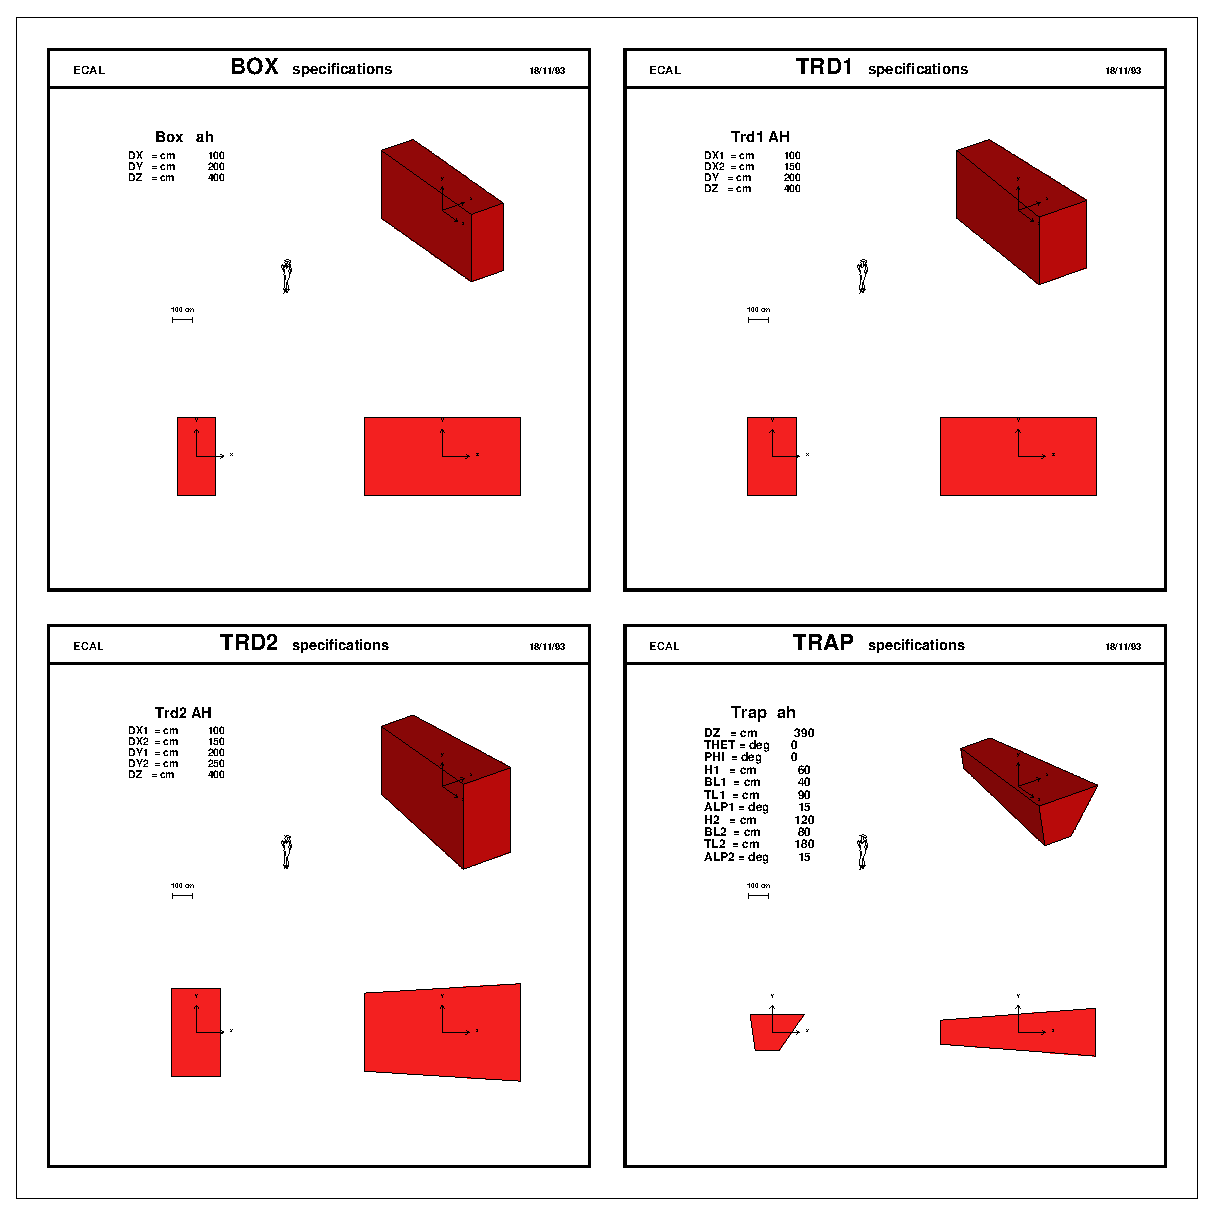
\epsfig{file=eps/geom050-1.eps,width=16cm}
      \caption{shapes {\tt BOX, TRD1, TRD2, TRAP}}
      \label{fg:geom050-1}
\end{figure}
\newpage
\begin{figure}[hbt]
\vspace{3cm}
      \centering
      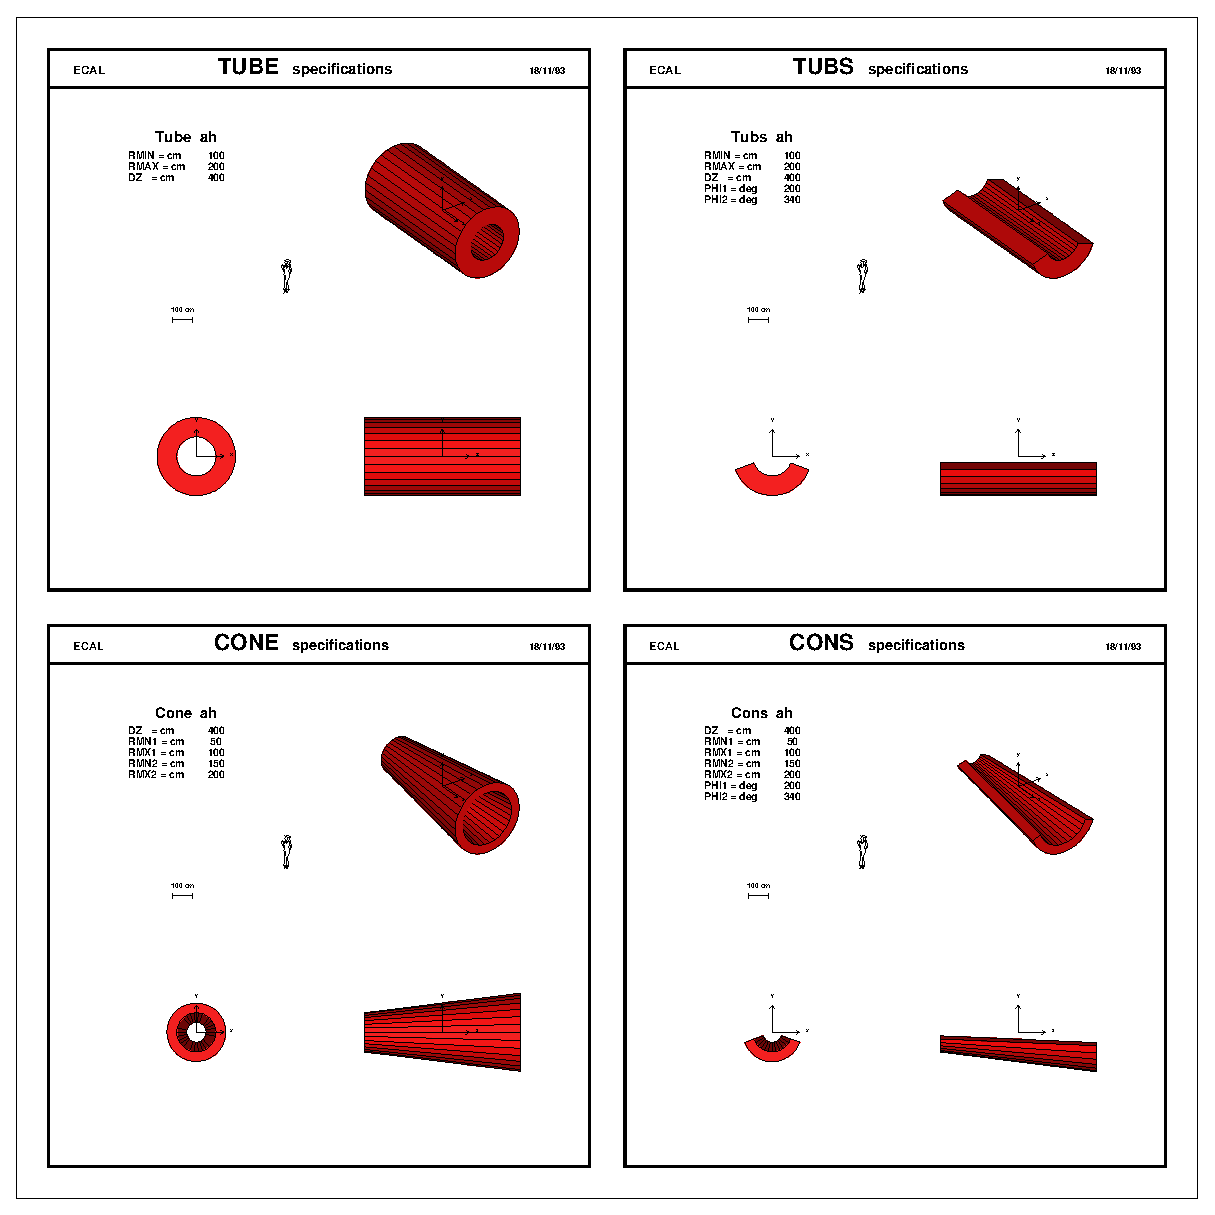
\epsfig{file=eps/geom050-2.eps,width=16cm}
      \caption{shapes {\tt TUBE, TUBS, CONE, CONS}}
      \label{fg:geom050-2}
\end{figure}
\newpage
\begin{figure}[hbt]
\vspace{3cm}
      \centering
      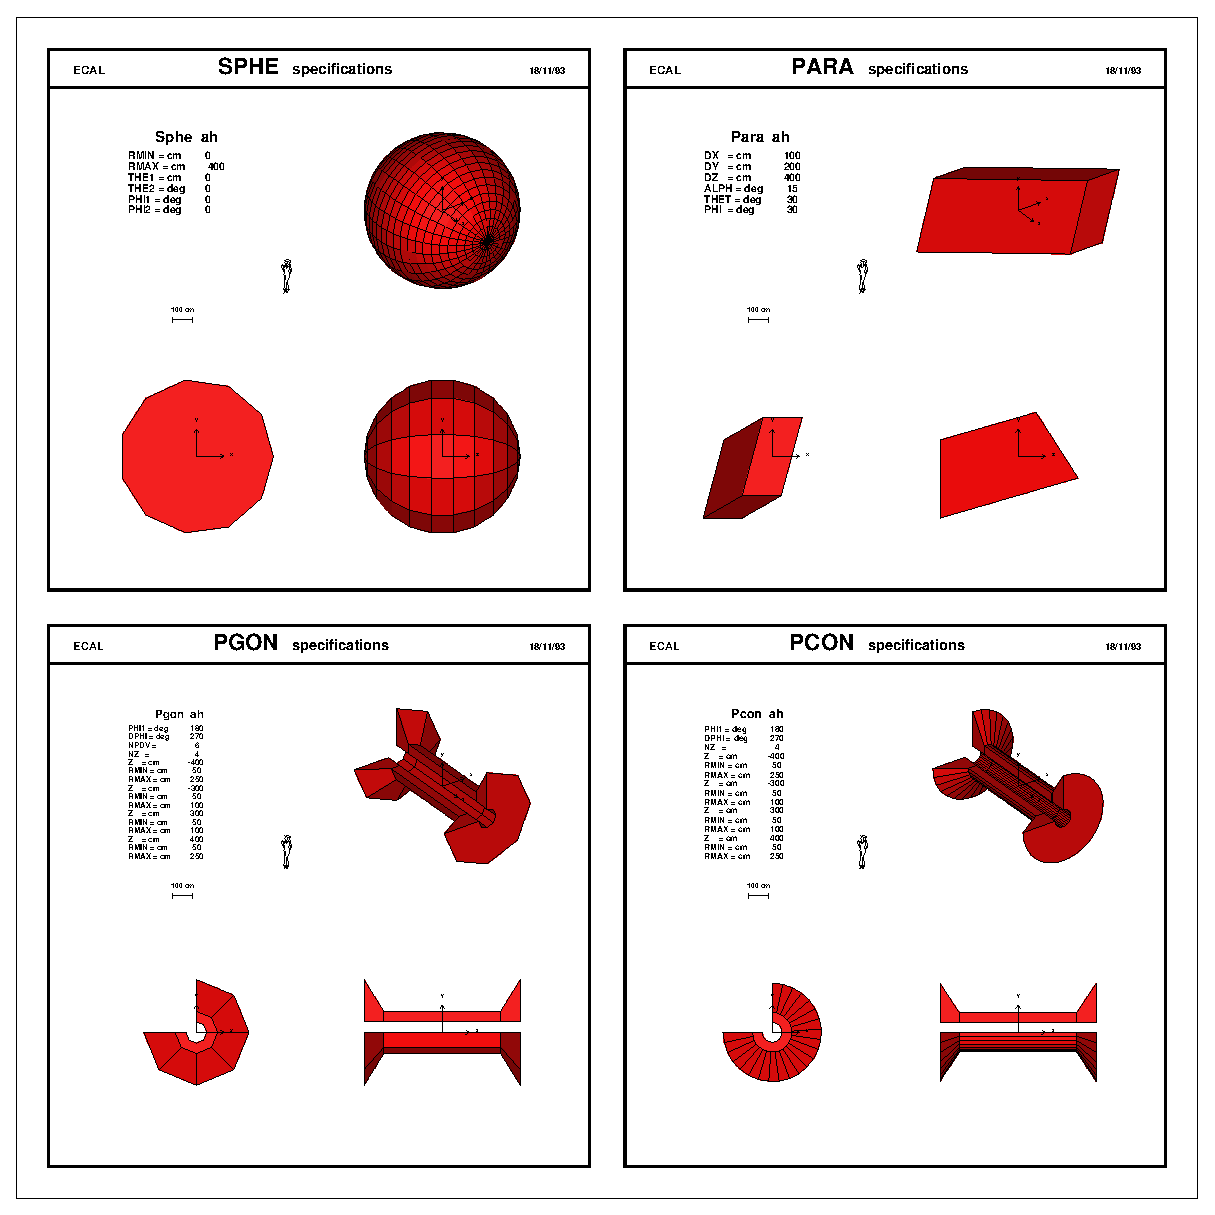
\epsfig{file=eps/geom050-3.eps,width=16cm}
      \caption{shapes {\tt PARA, SPHE, PGON, PCON}}
      \label{fg:geom050-3}
\end{figure}
\newpage
\begin{figure}[hbt]
\vspace{3cm}
      \centering
      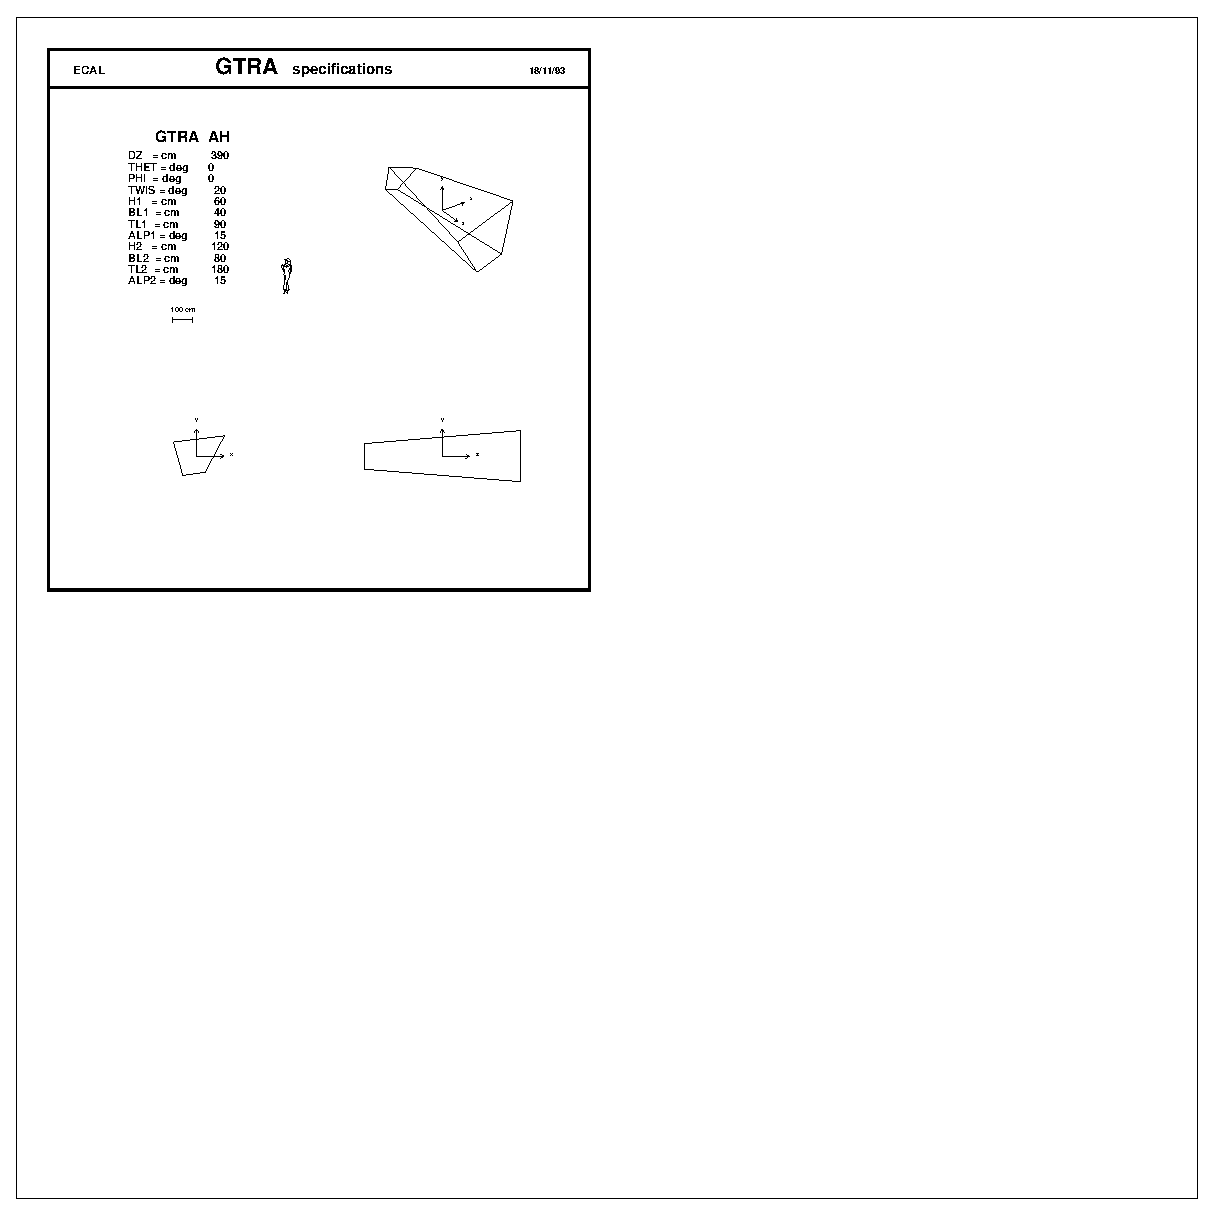
\epsfig{file=eps/geom050-4.eps,width=16cm}
      \caption{shapes {\tt GTRA}}
      \label{fg:geom050-4}
\end{figure}

%%%%%%%%%%%%%%%%%%%%%%%%%%%%%%%%%%%%%%%%%%%%%%%%%%%%%%%%%%%%%%%%%%%
%                                                                 %
%  GEANT manual in LaTeX form                              %
%                                                                 %
%  Michel Goossens (for translation into LaTeX)                   %
%  Version 1.00                                                   %
%  Last Mod. Jan 24 1991  1300   MG + IB                          %
%                                                                 %
%%%%%%%%%%%%%%%%%%%%%%%%%%%%%%%%%%%%%%%%%%%%%%%%%%%%%%%%%%%%%%%%%%%
\Origin{R.Brun,A.McPherson}
\Submitted{15.08.83}   \Revised{16.11.93}
\Version{Geant 3.16}   \Routid{GEOM100}
\Makehead{Creation of a volume}
 
\Shubr{GSVOLU}{(CHNAME,CHSHAP,NMED,PAR,NPAR,IVOLU*)}
Defines a volume with a given name, shape, tracking medium number
and shape parameters.

\begin{DLtt}{MMMMMMMM}
\item[CHNAME]  ({\tt CHARACTER*4}) volume name -- it must be unique;
\item[CHSHAP] ({\tt CHARACTER*4}) name of one of the {\tt GEANT} shapes;
\item[NMED]  ({\tt INTEGER}) tracking medium number for the volume --
if other volumes are positioned within this one, their tracking medium
replaces the one of the mother;
\item[PAR]   ({\tt REAL}) array containing the shape parameters;
\item[NPAR]  ({\tt INTEGER}) number of parameters -- if zero, then the
volume must be positioned via the routine \Rind{GSPOSP} indicating
the parameters for each copy (see {\tt [GEOM120]});
\item[IVOLU] ({\tt INTEGER}) internal volume number -- if $\leq 0$
an error condition has happened.
\end{DLtt}
 
If one of the parameters expressing a length is negative,
{\tt GEANT} will try to maximise its value in each copy, without
extending beyond the limits of the mother. This
facility can be used in conjunction with the
division of volumes using \Rind{GSDVN}, \Rind{GSDVT}, and \Rind{GSDVX}.
Restriction apply to this facility:
\begin{itemize}
\item the daughter should be positioned without a rotation matrix;
\item all shapes can be positioned within a similar shape with negative
parameters, but only in the centre of the mother;
\item boxes with negative parameters can be positioned in: box, {\tt TRD1},
{\tt TRD2} and {\tt TRAP} with $\theta = \phi = 0$;
\item {\tt HYPE}, {\tt ELTU} and {\tt CTUB} cannot have negative parameters;
\item {\tt PCON} and {\tt PGON} can only have 2 z planes.
\end{itemize}
{\bf Examples}
\begin{verbatim}
      DIMENSION PECAL(3)
      DATA PECAL/1.71,4.,0.2/
 
      CALL GSVOLU('ECAL','BOX ',1,PECAL,3,IVOLU)
\end{verbatim}
\Shubr{GPVOLU}{(IVOLU)}
Prints the volume parameters:
\begin{DLtt}{MMMM}
\item[IVOLU]  ({\tt INTEGER}) {\tt GEANT} number of the volume to print -- if
{\tt IVOLU} $\leq 0$, all volumes will be printed;
\end{DLtt}

%%%%%%%%%%%%%%%%%%%%%%%%%%%%%%%%%%%%%%%%%%%%%%%%%%%%%%%%%%%%%%%%%%%
%                                                                 %
%  GEANT manual in LaTeX form                                     %
%                                                                 %
%  Michel Goossens (for translation into LaTeX)                   %
%  Version 1.00                                                   %
%  Last Mod. Jan 24 1991  1300   MG + IB                          %
%                                                                 %
%%%%%%%%%%%%%%%%%%%%%%%%%%%%%%%%%%%%%%%%%%%%%%%%%%%%%%%%%%%%%%%%%%%
\Origin{R.Brun, A.McPherson}
\Submitted{15.08.83}              \Revised{16.11.93}
\Version{Geant 3.16}\Routid{GEOM110}

\Makehead{Positioning a volume inside its mother}

\Shubr{GSPOS}{(CHNAME,NR,CHMOTH,X,Y,Z,IROT,CHONLY)}
Places a copy of a volume previously defined by a call to \Rind{GSVOLU} 
inside its mother volume {\tt CHMOTH}.

\begin{DLtt}{MMMMMMMMMM}
\item[CHNAME] ({\tt CHARACTER*4}) name of the volume being positioned;
\item[NR] ({\tt INTEGER}) copy number of the volume {\tt CHNAME} being 
positioned;
\item[CHMOTH]({\tt CHARACTER*4}) name of the volume in which copy
{\tt NR} of {\tt CHNAME} is positioned;
\item[X] ({\tt REAL}) x position of the volume in the mother reference system;
\item[Y] ({\tt REAL}) y position of the volume in the mother reference system;
\item[Z] ({\tt REAL}) z position of the volume in the mother reference system;
\item[IROT] ({\tt INTEGER}) rotation matrix number
describing the orientation of the volume relative to
the coordinate system of the mother;
\item[CHONLY] ({\tt CHARACTER*4}) flag to indicate whether
a point found to be in this volume may also be in other volumes which
are not direct descendants of it -- possible values are {\tt ONLY} and
{\tt MANY}.
\end{DLtt}

The following points are important for a correct use of \Rind{GSPOS}:
\begin{itemize}
\item the position and rotation with which a volume is positioned are
relative to the mother reference system, that is to the reference system
of the volume which contains the copy being positioned. To see how the
reference system is defined for the {\tt GEANT} shapes, see {\tt [GEOM050]};
\item 
\Rind{GSPOS} can be called several times with the same name, to place 
multiple copies of the same volume either in the
same mother volume or in different ones.
The copy number parameter {\tt NR} is user defined, and it allows
the different copies of the same volume to be distinguished. The user is
free to assign any valid integer to this parameter. If two volumes
are positioned with the same copy number, it will be impossible to decide
in which one a particle is during tracking. If the same volume is positioned
twice inside the same mother with the same copy number, the parameters
of the second call to \Rind{GSPOS} will override the first ones for that
copy;
\item all the copies of a volume are identical: in particular they contain
all the same daughters recursively -- conversely, positioning a volume 
inside a mother will insert it in all the copies of that mother;
\item the volumes mentioned in the call must be already defined by a call
to \Rind{GSVOLU};
\item no volume can be positioned in a divided mother;
\item in case of positioning without rotation, {\tt IROT} should be set
to 0 -- note that this is faster than defining a unit matrix;
\item the first volume, containing all the apparatus, cannot be positioned;
\item if the {\tt CHONLY} flag is equal to {\tt ONLY}, the volume being
positioned should not overlap with any other volume except his mother
and his daughters and should not extend beyond the limits of its mother. 
In this case the search routines assume that, when a point
is found in this volume, the only further searching required is in its contents.
Other volumes at the same or higher levels
or in separate branches will not be looked at. The first volume must be 
{\tt ONLY};
\item if the {\tt CHONLY} flag is set to {\tt MANY}, a point found in
this volume can also be in another volume at the same or higher level or in
a different branch of the tree. To decide where a point is the following
algorithm is applied:
\begin{enumerate}
\item the tree is scanned {\it upward} until an {\tt ONLY} mother
with {\it positioned} contents (i.e. non-divided) is found;
\item all the branches of the tree descending from this volume are
scanned to find other volumes where the point may be;
\item a winner is selected among the candidates according to the
following rules:
\begin{itemize}
\item if one of the candidates is {\tt ONLY}, the point is declared in this
volume. If more than one candidate is {\tt ONLY} there is an error in the
geometry definition;
\item amongst several {\tt MANY} candidates, the one at the deepest level
is chosen;
\item amongst several {\tt MANY} candidates at the same level, the first one
found is chosen;
\end{itemize}
\end{enumerate}
Although a considerable effort has been put in making sure that the {\tt MANY}
option works properly and caters for all the possible cases, still it introduces
a considerable complication in the tracking and performance can be
rather poor.

Users should resort to this only when it is not possible to describe the
experimental setup with {\tt ONLY} volumes.
\end{itemize}

The data structure is so designed that, in any case, the parameters
of a volume and the information about the number and position of
its daughters are stored only once. This allows the creation of
very complex geometries without correspondingly large storage
requirements.

%%%%%%%%%%%%%%%%%%%%%%%%%%%%%%%%%%%%%%%%%%%%%%%%%%%%%%%%%%%%%%%%%%%
%                                                                 %
%  GEANT manual in LaTeX form                              %
%                                                                 %
%  Michel Goossens (for translation into LaTeX)                   %
%  Version 1.00                                                   %
%  Last Mod. Jan 24 1991  1300   MG + IB                          %
%                                                                 %
%%%%%%%%%%%%%%%%%%%%%%%%%%%%%%%%%%%%%%%%%%%%%%%%%%%%%%%%%%%%%%%%%%%
\Origin{R.Brun, F.Bruyant, M.Maire, A.McPherson}
\Submitted{15.08.83}               \Revised{18.11.93}
\Version{Geant 3.16}\Routid{GEOM120}
\Makehead{Positioning a volume inside its mother with parameters}

\Shubr{GSPOSP}{(CHNAME,NR,CHMOTH,X,Y,Z,IROT,CHONLY,PAR,NPAR)}

Position a copy of volume {\tt CHNAME} inside its mother {\tt CHMOTH}
assigning its parameters.

\begin{DLtt}{MMMMMMMMMM}
\item[CHNAME] ({\tt CHARACTER*4}) name of the volume being positioned;
\item[NR] ({\tt INTEGER}) copy number of the volume {\tt CHNAME} being
positioned;
\item[CHMOTH]({\tt CHARACTER*4}) name of the volume in which copy
{\tt NR} of {\tt CHNAME} is positioned;
\item[X] ({\tt REAL}) x position of the volume in the mother reference system;
\item[Y] ({\tt REAL}) y position of the volume in the mother reference system;
\item[Z] ({\tt REAL}) z position of the volume in the mother reference system;
\item[IROT] ({\tt INTEGER}) rotation matrix number
describing the orientation of the volume relative to
the coordinate system of the mother;
\item[CHONLY] ({\tt CHARACTER*4}) flag to indicate whether
a point found to be in this volume may also be in other volumes which
are not direct descendants of it -- possible values are {\tt ONLY} and
{\tt MANY};
\item[PAR] ({\tt REAL}) array of parameters for the volume being positioned;
\item[NPAR] ({\tt INTEGER}) number of parameters.
\end{DLtt}

It is often the case in a detector to have a family of similar objects,
differing only by their dimensions. A typical example are the crystals of
an electromagnetic calorimeter. In this case it is convenient and logically
consistent to give them all the same name, but assign to each copy a different
set of parameters.

This can be done defining the volume with 0 parameters through the routine
\Rind{GSVOLU} and then assigning the parameters to each copy via the routine
\Rind{GSPOSP}.

\Rind{GSPOSP} is similar in all other aspects to \Rind{GSPOS} and the user is
referred to the description of this routine for more information. An obvious
limitation is that a volume defined with 0 parameters can only be positioned
via \Rind{GSPOSP}, because otherwise its dimensions will be undefined.

%%%%%%%%%%%%%%%%%%%%%%%%%%%%%%%%%%%%%%%%%%%%%%%%%%%%%%%%%%%%%%%%%%%
%                                                                 %
%  GEANT manual in LaTeX form                                     %
%                                                                 %
%  Michel Goossens (for translation into LaTeX)                   %
%  Version 1.00                                                   %
%  Last Mod. Jan 24 1991  1300   MG + IB                          %
%                                                                 %
%%%%%%%%%%%%%%%%%%%%%%%%%%%%%%%%%%%%%%%%%%%%%%%%%%%%%%%%%%%%%%%%%%%
\Origin{R.Brun, A.McPherson}
\Submitted{29.09.83}             \Revised{18.11.93}
\Version{Geant 3.16}\Routid{GEOM130}
\Makehead{Division of a volume into a given number of cells}

\Shubr{GSDVN}{(CHNAME,CHMOTH,NDIV,IAXIS)}

Divide a volume in a given number of parts along a direction. 

\begin{DLtt}{MMMMMMMM}
\item[CHNAME] ({\tt CHARACTER*4}) a unique name for the volume to be generated
by subdivision of the mother volume;
\item[CHMOTH] ({\tt CHARACTER*4}) volume that has to be subdivided;
\item[NDIV] ({\tt INTEGER}) number of divisions into which the mother volume 
is to be divided;
\item[IAXIS] ({\tt INTEGER}) {\it axis} of the division.
\end{DLtt}

The volumes resulting from a division are true volumes in
the {\tt GEANT} sense, with the only limitation that they cannot be
positioned. They can have daughters and they can still be divided in turn.
Different divisions are distinguished by a different division number,
much the same as different copy of the same volume by the copy number.
Every operation performed on a division cell (positioning or further division),
is automatically propagated to all divisions cells of the same mother.

The kind of the division is indicated by the {\tt IAXIS} argument. 
The
allowed values of {\tt IAXIS} and the resulting divisions are shown in
figs. \ref{fg:geom130-1}, \ref{fg:geom130-2}, \ref{fg:geom130-3}, 
\ref{fg:geom130-4}, where the pictures in the first column correspond to 
an {\tt IAXIS} value equal to 1, the second column to {\tt IAXIS} = 2, 
and the third column to {\tt IAXIS} = 3 respectivly.
The
basic constraint imposed by the {\tt GEANT} geometry is that the result
of a division is a volume which can be described in terms of the basic 
shapes.

The local coordinate system of the divisions is parallel to the
system of the mother in case of divisions obtained by parallel planes or
concentric divisions. In the case of parallel axes the coordinate system
is shifted so that it is in the centre of the division.
In case of $\phi$ divisions produced by planes
passing through the axis of a volume with axial symmetry ({\tt TUBE, TUBS,
CONE, CONS, PGON, PCON, SPHE}), the local coordinate systems will be 
rotated so that the x axis passes through the centre of the division.

This routine allows the user to generate a large number of identical
volumes filling a defined volume. The material of the slices is inherited
from the mother.

It may happen that the different divisions of a volume have different
dimensions. In this case, if a volume has to be positioned in each division, 
its dimensions must be different according to the division number. This can
be obtained in some special cases giving to the dimension of the
volume which has to vary in order to fit into the different mothers,
the value of -1 in the call to
\Rind{GSVOLU} which defines it. As explained in {\tt [GEOM050]}, {\tt GEANT}
will take care to assign to this dimension the maximum value in order to
fill the current mother.

What can be done with division can be done also, in most cases, explicitly
positioning all the copies. Users must be aware, however, that divisions
offer the best performance in tracking of all {\tt GEANT} geometrical
constructs, and they should be used instead of positioning whenever
possible in the definition of objects.

\newpage
\begin{figure}[hbt]
      \centering
      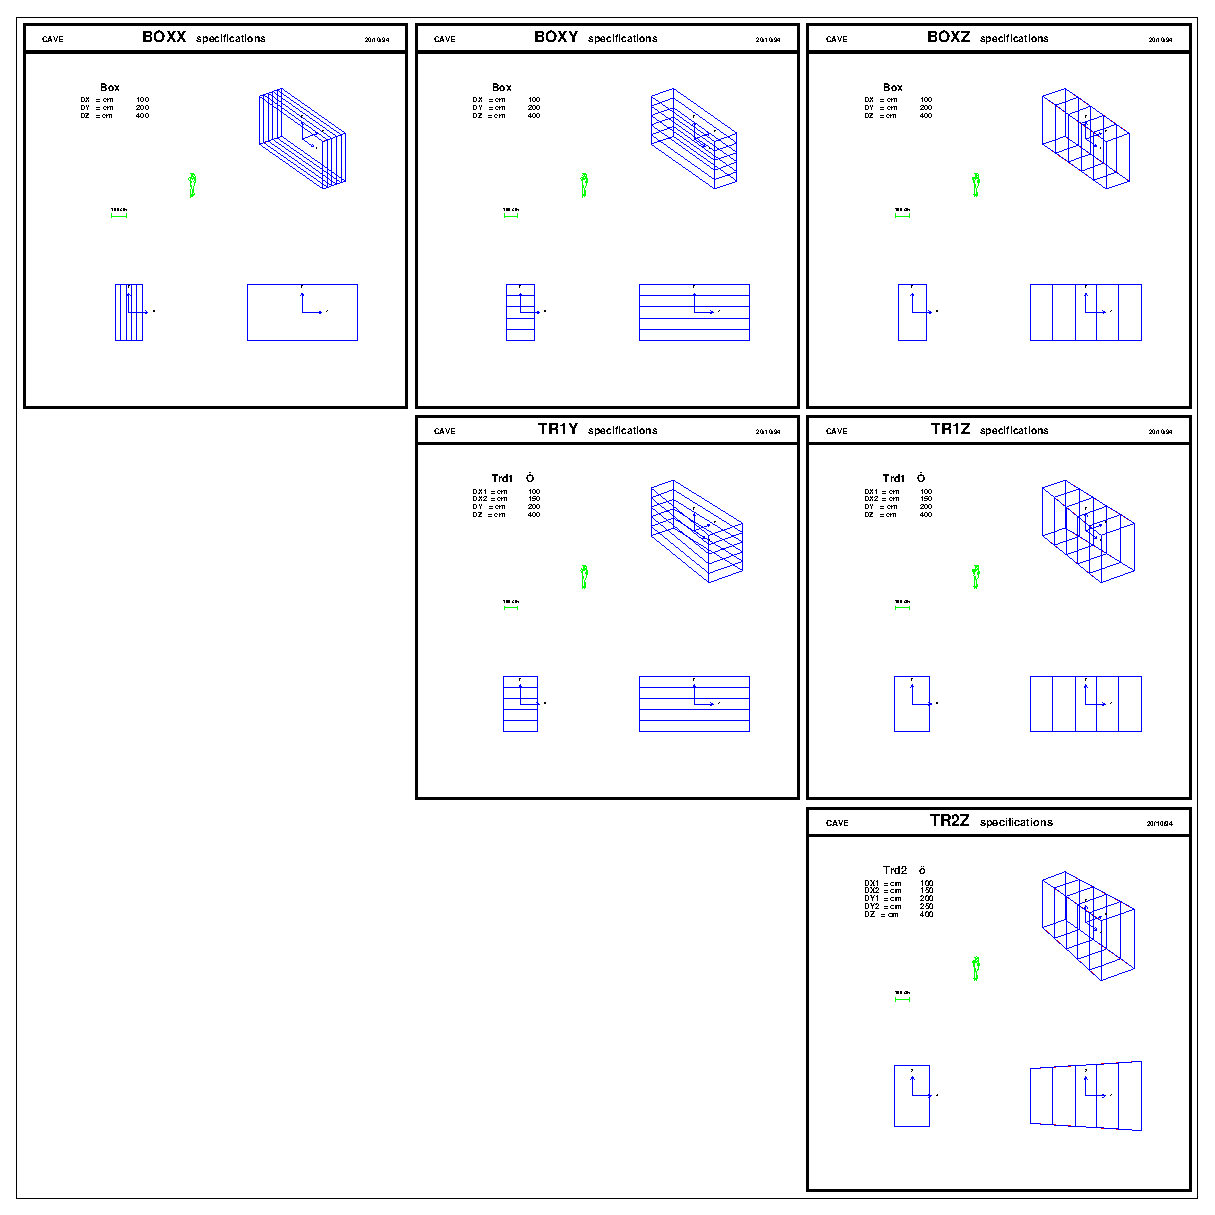
\epsfig{file=eps/geom130-1.eps,width=16cm}
      \caption{shapes {\tt BOX, TRD1, TRD2}}
      \label{fg:geom130-1}
\end{figure}
\newpage
\begin{figure}[hbt]
      \centering
      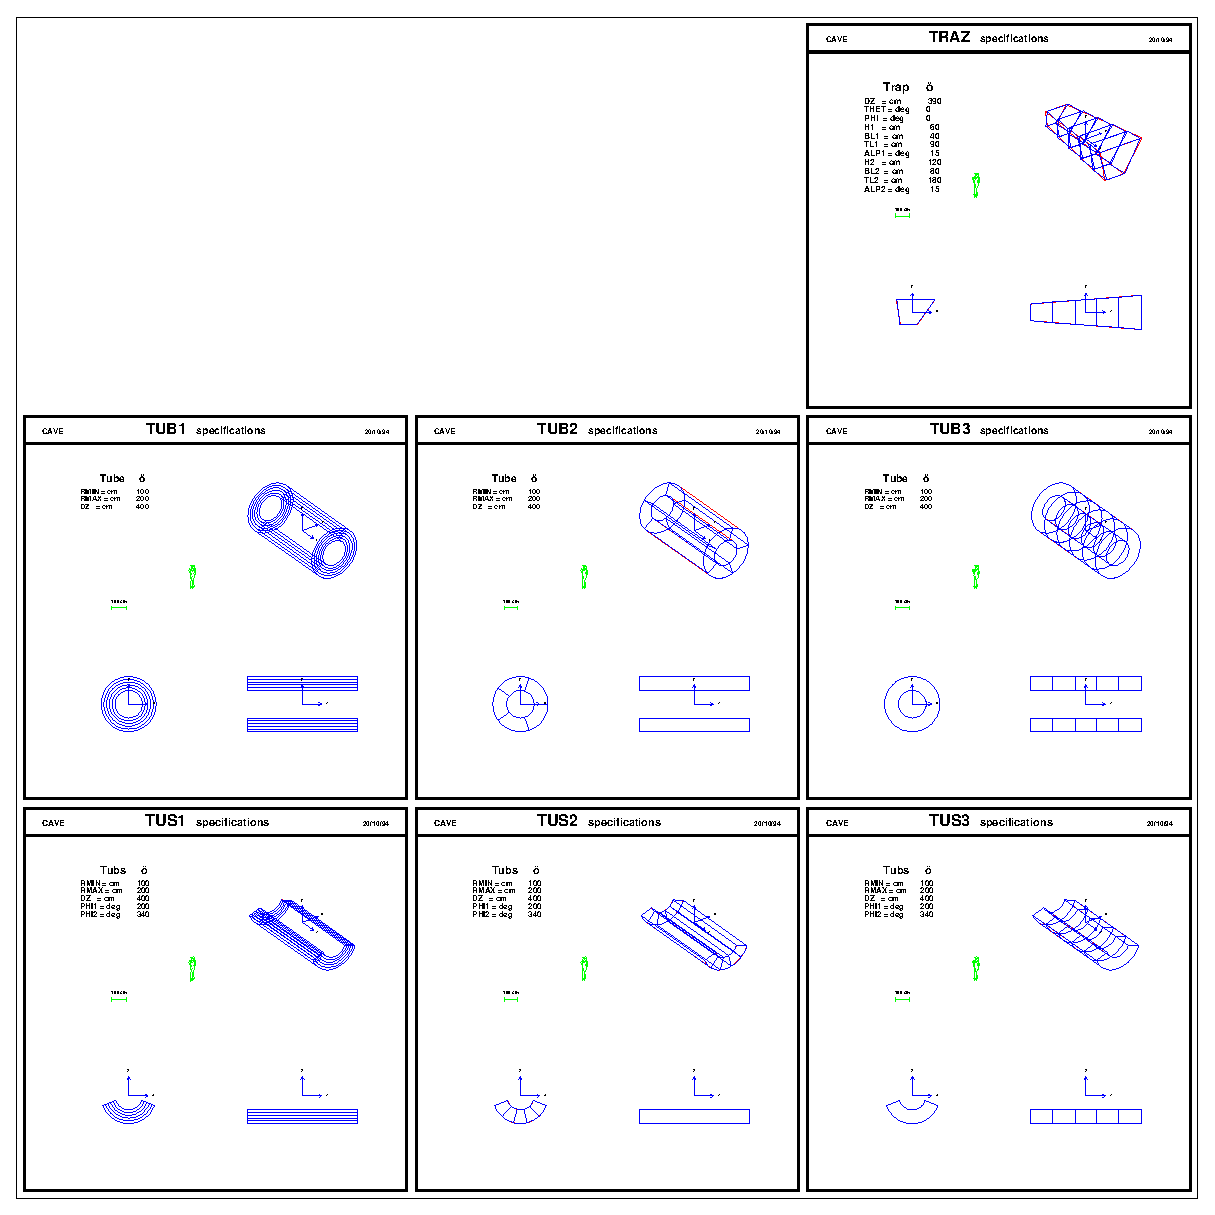
\epsfig{file=eps/geom130-2.eps,width=16cm}
      \caption{shapes {\tt TRAP, TUBE, TUBS}}
      \label{fg:geom130-2}
\end{figure}
\newpage
\begin{figure}[hbt]
      \centering
      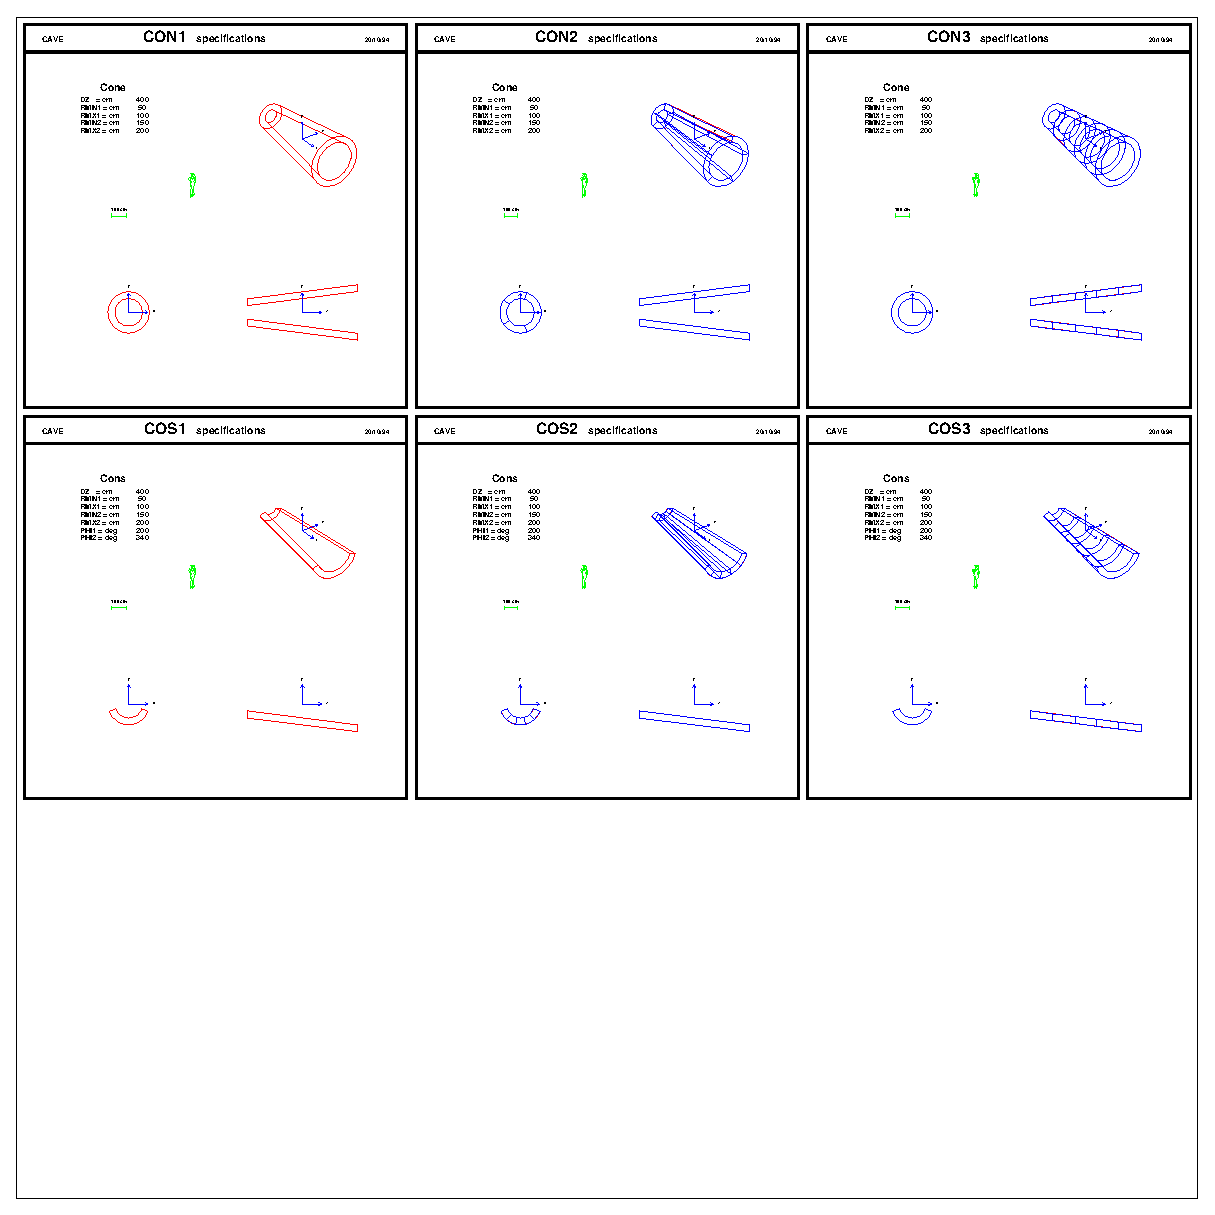
\epsfig{file=eps/geom130-3.eps,width=16cm}
      \caption{shapes {\tt CONE, CONS}}
      \label{fg:geom130-3}
\end{figure}
\newpage
\begin{figure}[hbt]
      \centering
      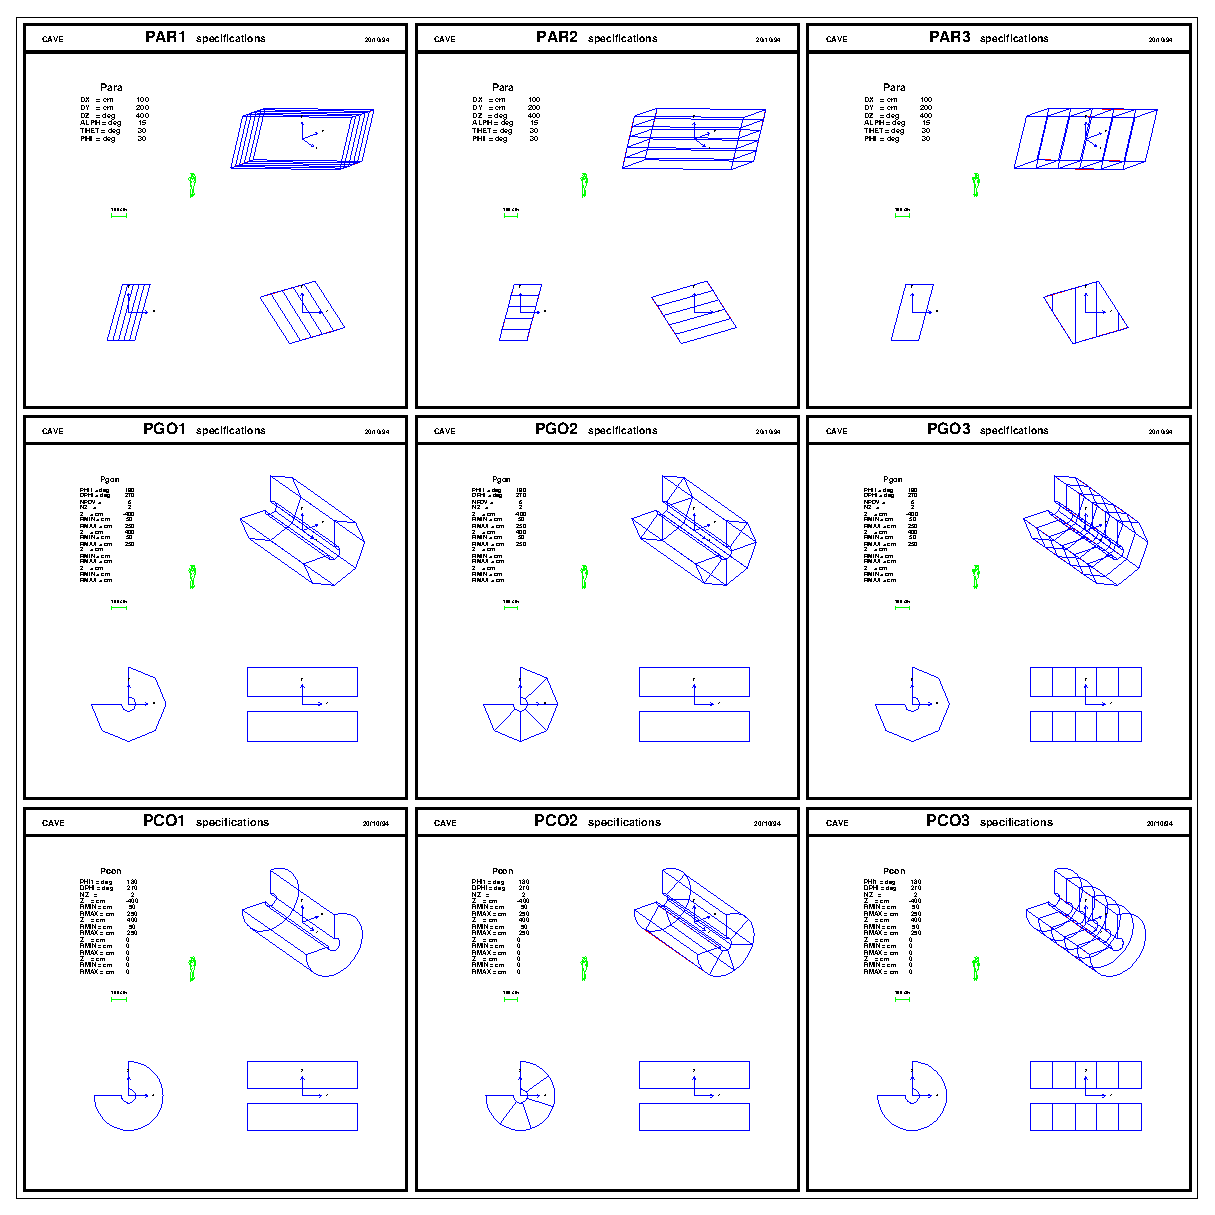
\epsfig{file=eps/geom130-4.eps,width=16cm}
      \caption{shapes {\tt PARA, PGON, PCON}}
      \label{fg:geom130-4}
\end{figure}

%%%%%%%%%%%%%%%%%%%%%%%%%%%%%%%%%%%%%%%%%%%%%%%%%%%%%%%%%%%%%%%%%%%
%                                                                 %
%  GEANT manual in LaTeX form                              %
%                                                                 %
%  Michel Goossens (for translation into LaTeX)                   %
%  Version 1.00                                                   %
%  Last Mod. Jan 24 1991  1300   MG + IB                          %
%                                                                 %
%%%%%%%%%%%%%%%%%%%%%%%%%%%%%%%%%%%%%%%%%%%%%%%%%%%%%%%%%%%%%%%%%%%
\Origin{F.Bruyant, A.McPherson, M.Maire}
\Submitted{17.12.83}       \Revised{18.11.93}
\Version{Geant 3.16}\Routid{GEOM140}
\Makehead{Division of a Volume into cells of a given size}

This routine creates new volumes from a mother 
by divisions of a given step.

\Shubr{GSDVT}{(CHNAME,CHMOTH,STEP,IAXIS,NUMED,NDVMX)}

\begin{DLtt}{MMMMMMMM}
\item[CHNAME] ({\tt CHARACTER*4}) a unique name for the volume to be generated
by subdivision of the mother volume;
\item[CHMOTH] ({\tt CHARACTER*4}) volume that has to be subdivided;
\item[STEP] ({\tt REAL}) size of the divisions -- this value can be in 
centimeters or degrees according to the value of {\tt IAXIS};
\item[IAXIS] ({\tt INTEGER}) {\it axis} of the division.
\item[NUMED] ({\tt INTEGER}) medium number of the divisions -- this can be 
different from the one of the mother, as the division cells may leave a
portion of the mother undivided (see below) --
if {\tt NUMED} $\leq 0$  the medium of the mother;
\item[NDVMX] ({\tt INTEGER}) expected (maximum) number of divisions -- if
$ \leq 0 $ or $ > 255 $, 255 is assumed.
\end{DLtt}

The full range of the mother will be divided
in sections of the user supplied step. If the step is such that the mother
cannot be divided exactly, the largest possible number
of divisions will be generated, the excess space will be equally
divided between each end of the range of the mother. These extra
spaces will be assumed to belong to the mother.

For more information on the division in general, see {\tt [GEOM130]}.

%%%%%%%%%%%%%%%%%%%%%%%%%%%%%%%%%%%%%%%%%%%%%%%%%%%%%%%%%%%%%%%%%%%
%                                                                 %
%  GEANT manual in LaTeX form                              %
%                                                                 %
%  Michel Goossens (for translation into LaTeX)                   %
%  Version 1.00                                                   %
%  Last Mod. Jan 24 1991  1300   MG + IB                          %
%                                                                 %
%%%%%%%%%%%%%%%%%%%%%%%%%%%%%%%%%%%%%%%%%%%%%%%%%%%%%%%%%%%%%%%%%%%
\Origin{R.Brun, F.Bruyant, A.McPherson}
\Submitted{17.12.83}               \Revised{18.11.93}
\Version{Geant 3.16}\Routid{GEOM150}
\Makehead{Division of a volume - general case}

\Shubr{GSDVX}{(CHNAME,CHMOTH,NDIV,IAXIS,STEP,C0,NUMED,NDVMAX)}

Divide a volume in a given number of parts along a direction, with
a given step starting from an offset.

\begin{DLtt}{MMMMMMMM}
\item[CHNAME] ({\tt CHARACTER*4}) a unique name for the volume to be generated
by subdivision of the mother volume;
\item[CHMOTH] ({\tt CHARACTER*4}) volume that has to be subdivided;
\item[NDIV] ({\tt INTEGER}) number of divisions into which the mother volume
is to be divided;
\item[IAXIS] ({\tt INTEGER}) {\it axis} of the division.
\item[STEP] ({\tt REAL}) size of the divisions -- this value can be in
centimeters or degrees according to the value of {\tt IAXIS};
\item[C0] ({\tt REAL}) offset where division should start -- this value can be 
in centimeters or degrees according to the value of {\tt IAXIS};
\item[NUMED] ({\tt INTEGER}) medium number of the divisions -- this can be
different from the one of the mother, as the division cells may leave a
portion of the mother undivided (see below) --
if {\tt NUMED} $\leq 0$  the medium of the mother;
\item[NDVMX] ({\tt INTEGER}) expected (maximum) number of divisions -- if
$ \leq 0 $ or $ > 255 $, 255 is assumed.
\end{DLtt}

For more information on the division mechanism, see {\tt [GEOM130]} and
{\tt [GEOM140]}. For the moment either
{\tt NDIV} or {\tt STEP} must be set negative or 0, so that they
will be computed from the {\tt CHMOTH}'s size.
The case with both {\tt NDIV} and {\tt STEP}
positive is not coded yet. It would permit leaving different
gaps at both ends of the
{\tt CHMOTH}.

Provisionally the code consists of a call to either \Rind{GSDVN2} or
\Rind{GSDVT2}.

\Shubr{GSDVN2}{(CHNAME,CHMOTH,NDIV,IAXIS,C0,NUMED)}

Divide a volume in a given number of parts along a direction, 
starting from an offset.

\begin{DLtt}{MMMMMMMM}
\item[CHNAME] ({\tt CHARACTER*4}) a unique name for the volume to be generated
by subdivision of the mother volume;
\item[CHMOTH] ({\tt CHARACTER*4}) volume that has to be subdivided;
\item[NDIV] ({\tt INTEGER}) number of divisions into which the mother volume
is to be divided;
\item[IAXIS] ({\tt INTEGER}) {\it axis} of the division.
\item[C0] ({\tt REAL}) offset where division should start -- this value can be 
in centimeters or degrees according to the value of {\tt IAXIS};
\item[NUMED] ({\tt INTEGER}) medium number of the divisions -- this can be
different from the one of the mother, as the division cells may leave a
portion of the mother undivided (see below) --
if {\tt NUMED} $\leq 0$  the medium of the mother;
\end{DLtt}

The divisions start at the user specified coordinate value
and extend to the end of the volume. The range from this offset to
the upper coordinate limit of the mother volume will be divided
into the supplied number of cells. 
In the case of 
$\phi$ division of a complete tube or cone, the whole 360 degrees
will be divided into the user-supplied number of slices no matter
what the origin is. Specifying an origin for the division, in this
case, just moves the
division boundaries. This can be useful to avoid a rotation.
In all other cases the search routines will
assume that a point is in the mother if the coordinate value is
less than the value of the supplied offset.

\Shubr{GSDVT2}{(CHNAME,CHMOTH,STEP,IAXIS,C0,NUMED,NDVMX)}

Divide a volume along a direction with a given step starting from an offset.

\begin{DLtt}{MMMMMMMM}
\item[CHNAME] ({\tt CHARACTER*4}) a unique name for the volume to be generated
by subdivision of the mother volume;
\item[CHMOTH] ({\tt CHARACTER*4}) volume that has to be subdivided;
\item[STEP] ({\tt REAL}) size of the divisions -- this value can be in
centimeters or degrees according to the value of {\tt IAXIS};
\item[IAXIS] ({\tt INTEGER}) {\it axis} of the division;
\item[C0] ({\tt REAL}) offset where division should start -- this value can be
in centimeters or degrees according to the value of {\tt IAXIS};
\item[NUMED] ({\tt INTEGER}) medium number of the divisions -- this can be
different from the one of the mother, as the division cells may leave a
portion of the mother undivided (see below) --
if {\tt NUMED} $\leq 0$  the medium of the mother;
\item[NDVMX] ({\tt INTEGER}) expected (maximum) number of divisions -- if
$ \leq 0 $ or $ > 255 $, 255 is assumed.
\end{DLtt}

The division start at the user-specified coordinate value
and extend to the end of the volume. The range from origin to
upper coordinate limit of the mother volume is divided
in sections of the user supplied step. If the step is such that
the range of the mother cannot be filled with cells, the largest
possible number of cells is created.
The excess space up to the end
of the mother volume will be assumed to belong to the mother.

In the case of 
$\phi$ division of a complete tube or cone, the whole 360 degrees
will be filled with slices, no matter
what the origin is. Specifying an origin for the division, in this
case, just moves the
division boundaries. This can be useful to avoid a rotation.

In all other cases the search routines will
assume a point is just in the mother if the coordinate value is
less than the value of the user supplied origin.

%%%%%%%%%%%%%%%%%%%%%%%%%%%%%%%%%%%%%%%%%%%%%%%%%%%%%%%%%%%%%%%%%%%
%                                                                 %
%  GEANT manual in LaTeX form                              %
%                                                                 %
%  Michel Goossens (for translation into LaTeX)                   %
%  Version 1.00                                                   %
%  Last Mod. Jan 24 1991  1300   MG + IB                          %
%                                                                 %
%%%%%%%%%%%%%%%%%%%%%%%%%%%%%%%%%%%%%%%%%%%%%%%%%%%%%%%%%%%%%%%%%%%
\Origin{R.Brun,F.Bruyant,A.McPherson}
\Submitted{01.11.83}                     \Revised{18.11.93}
\Version{Geant 3.16}\Routid{GEOM199}
\Makehead{The volume data structure -- JVOLUM}

\section{The data structure {\tt JVOLUM} and {\tt JGPAR}}

The meaning of the variables in the data structure {\tt JVOLUM} shown
in fig. \ref{fg:geom199-1}
is the following:

\begin{DLtt}{MMMMMMMM}
\item[ISEARC] search flag {\tt [GEOM400], [GEOM410]}:
\begin{DLtt}{MMMM}
\item[$=$0] volume positioning order or ordering by \Rind{GSNEXT}/\Rind{GSNEAR};
\item[$<$0] binary search as defined by \Rind{GSORD};
\item[$>$0] user ordering \Rind{GSUNEA}/\Rind{GUNEAR};
\end{DLtt}
\item[ISHAPE] system shape number (see {\tt [GEOM050]};
\item[NIN] number of volumes contained in the mother volume --
if negative the volume is divided;
\item[NMED] medium number for the volume;
\item[NPAR] number of shape parameters;
\item[NATT] number of attributes;
\item[PAR] array of shape parameters;
\item[IAT] array of attributes;
\item[IAXIS] direction of the division (see {\tt [GEOM130]});
\item[IVO] system volume number;
\item[NDIV] number of divisions ({\tt -NDVMX}, if computed dynamically,
see {\tt [GEOM140]});
\item[C0] coordinate value at which the division starts;
\item[STEP] coordinate step for the division;
\item[NR] user copy number;
\item[IROT] rotation matrix number defining the orientation of the volume
with respect to the mother reference system;
\item[X,Y,Z] position of the volume with respect to the mother reference
system;
\item[KONLY] {\tt ONLY/MANY} flag, see {\tt [GEOM110]} for more information;
\end{DLtt}
 
\begin{figure}[hbt]
     \centering
     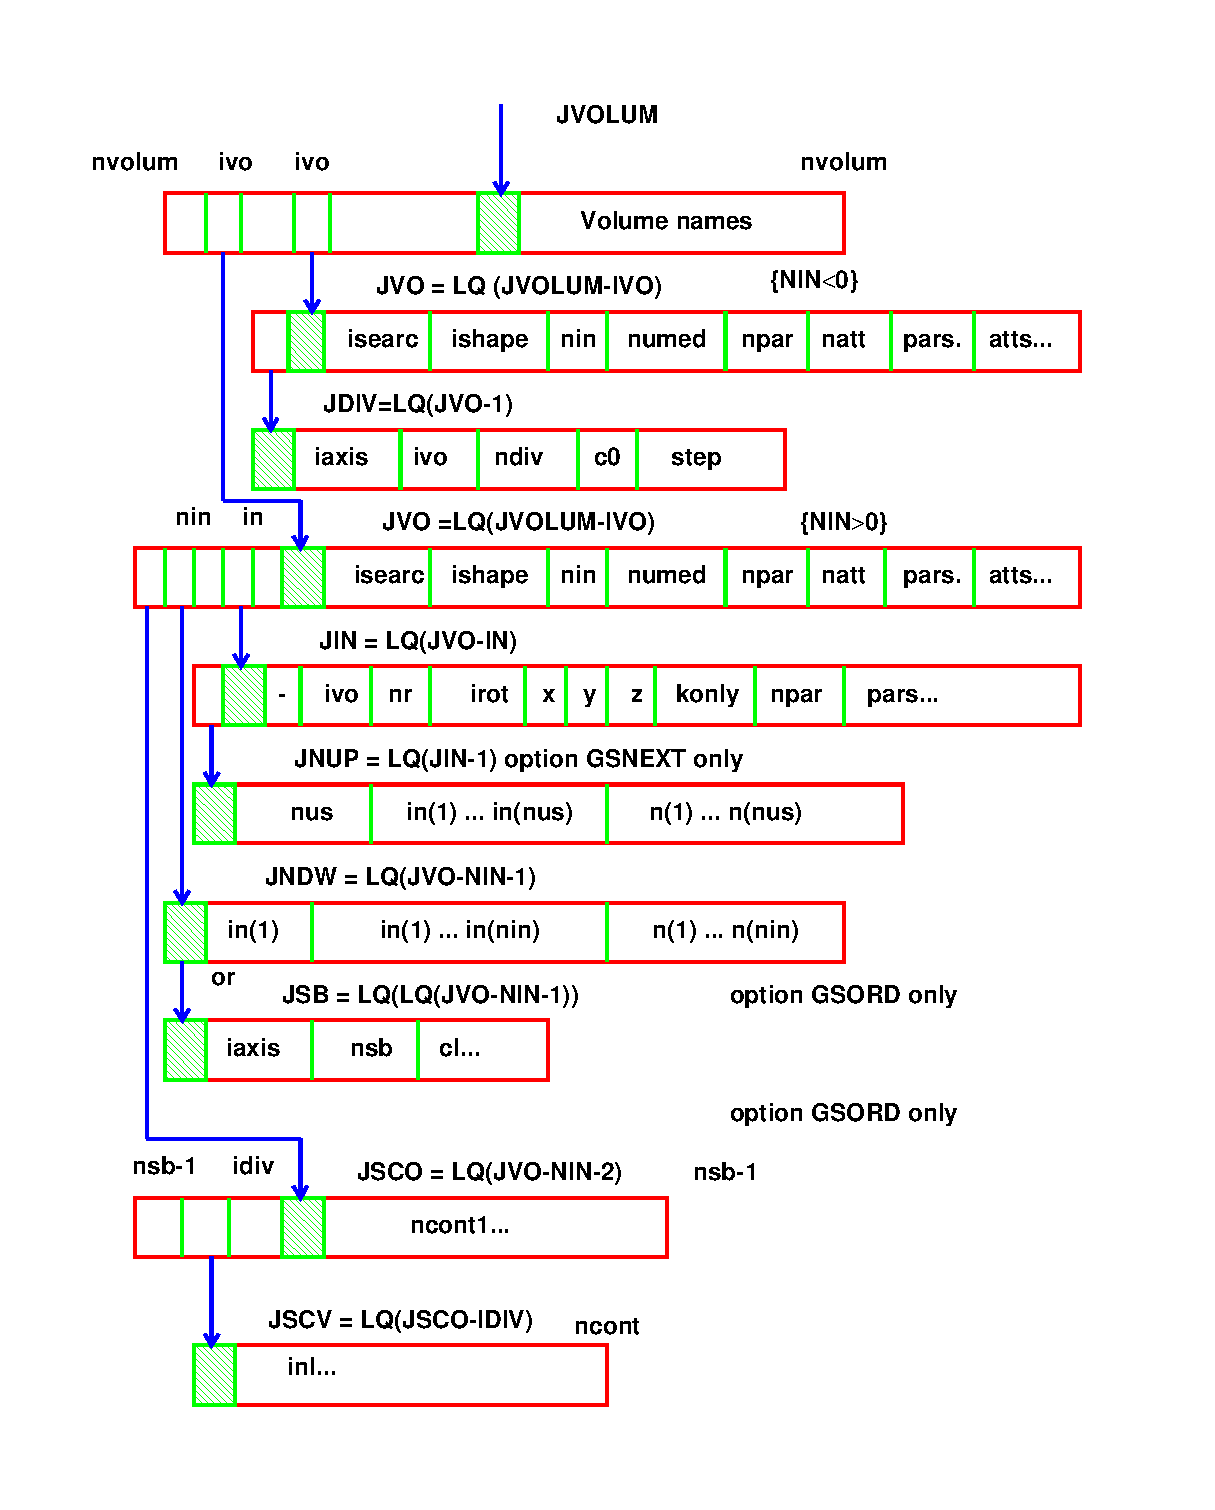
\epsfig{file=eps/geom199-1.eps,width=14cm}
     \caption{Example of geometrical tree structure}
     \label{fg:geom199-1}
\end{figure}

%%%%%%%%%%%%%%%%%%%%%%%%%%%%%%%%%%%%%%%%%%%%%%%%%%%%%%%%%%%%%%%%%%%
%                                                                 %
%  GEANT manual in LaTeX form                              %
%                                                                 %
%  Michel Goossens (for translation into LaTeX)                   %
%  Version 1.00                                                   %
%  Last Mod. Jan 24 1991  1300   MG + IB                          %
%                                                                 %
%%%%%%%%%%%%%%%%%%%%%%%%%%%%%%%%%%%%%%%%%%%%%%%%%%%%%%%%%%%%%%%%%%%
\Origin{R.Brun, F.Carena}
\Submitted{01.06.83}             \Revised{14.12.93}
\Version{Geant 3.16}\Routid{GEOM200}
\Makehead{Rotation matrices}

The relative position of a volume inside its mother is expressed in
{\tt GEANT} by a translation vector and a rotation matrix which are 
arguments of the routines \Rind{GSPOS} and \Rind{GSPOSP}. The rotation
matrix expresses the transformation from the {\tt M}other {\tt R}eference
{\tt S}ystem to the {\tt D}aughter {\tt R}eference {\tt S}ystem.

A rotation matrix is described to {\tt GEANT} by giving the polar and
azimuthal angles of the axes of the {\tt DRS} ($x', y', z'$) in the
{\tt MRS} via the routine \Rind{GSROTM}.

\Shubr{GSROTM}{(IROT,THETA1,PHI1,THETA2,PHI2,THETA3,PHI3)}
\begin{DLtt}{MMMMMMMM}
\item[IROT] ({\tt INTEGER}) number of the rotation matrix;
\item[THETA1] ({\tt REAL}) polar angle for axis $x'$;
\item[PHI1] ({\tt REAL}) azimuthal angle for axis $x'$;
\item[THETA2] ({\tt REAL}) polar angle for axis $y'$;
\item[THI2] ({\tt REAL}) azimuthal angle for axis $y'$;
\item[THETA3] ({\tt REAL}) polar angle for axis $z'$;
\item[PHI3] ({\tt REAL}) azimuthal angle for axis $z'$.
\end{DLtt}
Stores rotation matrix {\tt IROT} in the data structure {\tt JROTM}. If the
matrix is not orthonormal, it will be corrected by setting $y' \perp x'$ and
then $z' = x' \times y'$. A warning message is printed in this case.

{\bf Note:}
the angles {\tt THETA} and {\tt PHI} must be given in degrees.
 
\section*{Examples of use}
The unit matrix is defined in the following way:

\[
\left . \begin{array}{lcl}
x' & \| & x \\
y' & \| & y \\
z' & \| & z
\end{array} \right \}
\Rightarrow
\left \{
\begin{array}{lcr@{\mbox{\hspace{3mm};\hspace{8mm}}}lcr}
\theta_1 & = & 90^{\circ} & \phi_1 & = & 0^{\circ} \\
\theta_2 & = & 90^{\circ} & \phi_2 & = & 90^{\circ} \\
\theta_3 & = & 0^{\circ} & \phi_3 & = & 0^{\circ} 
\end{array} \right .
\]

This is just an example. There is in fact no need to define a unit rotation
matrix. Giving the value 0 to the rotation matrix number in the call to
\Rind{GSPOS} and \Rind{GSPOSP} is equivalent to a positioning without 
rotation and it improves tracking performance.

The result of a $90^{\circ}$ counterclockwise rotation around $z$, followed
by a $90^{\circ}$ counterclockwise rotation around the new $x$ is a cyclic
shift of the axes: $x \rightarrow z', \; y \rightarrow x', \; z \rightarrow  
y'$. This is expressed by the following rotation matrix:

\[
\left . \begin{array}{lcl}
x' & \| & y \\
y' & \| & z \\
z' & \| & x
\end{array} \right \}
\Rightarrow
\left \{
\begin{array}{lcr@{\mbox{\hspace{3mm};\hspace{8mm}}}lcr}
\theta_1 & = & 90^{\circ} & \phi_1 & = & 90^{\circ} \\
\theta_2 & = & 0^{\circ} & \phi_2 & = & 0^{\circ} \\
\theta_3 & = & 90^{\circ} & \phi_3 & = & 0^{\circ} 
\end{array} \right .
\]

Sometimes the rotation matrix is known or it can be constructed. In this case
the arguments to the routine \Rind{GSROTM} can be calculated with the help
of the routine \Rind{GFANG} in the following way:

\begin{verbatim}
      DIMENSION ROTMAT(3,3), ROWMAT(3), PHI(3), THETA(3)
      LOGICAL ROTATE
      .
      .
      .
      DO 10 I=1,3
         ROWMAT(1) = ROTMAT(I,1)
         ROWMAT(2) = ROTMAT(I,2)
         ROWMAT(3) = ROTMAT(I,3)
         CALL GFANG(ROWMAT,COSTH,SINTH,COSPH,SINPH,ROTATE)
         THETA(I) = ATAN2(SINTH,COSTH)
         PHI(I)   = ATAN2(SINPH,COSPH)
  10  CONTINUE
      .
      . {\sl Transform to degrees}
      .
      CALL GSROTM(IROT,THETA(1),PHI(1),THETA(2),PHI(2),THETA(3),PHI(3))
\end{verbatim}
 
\Shubr{GPROTM}{(IROT)}
Prints the rotation matrix elements and angles.
\begin{DLtt}{MMMMMMMM}
\item[IROT]  ({\tt INTEGER}) rotation matrix number: if {\tt IROT}=0 all
rotation matrixes will be printed, if {\tt IROT}$<$0, matrix number
{\tt |IROT|} will be printed without header information.
\end{DLtt}
 

%%%%%%%%%%%%%%%%%%%%%%%%%%%%%%%%%%%%%%%%%%%%%%%%%%%%%%%%%%%%%%%%%%%
%                                                                 %
%  GEANT manual in LaTeX form                              %
%                                                                 %
%  Michel Goossens (for translation into LaTeX)                   %
%  Version 1.00                                                   %
%  Last Mod. Jan 24 1991  1300   MG + IB                          %
%                                                                 %
%%%%%%%%%%%%%%%%%%%%%%%%%%%%%%%%%%%%%%%%%%%%%%%%%%%%%%%%%%%%%%%%%%%
\Origin{R.Brun}
\Submitted{01.11.78}     \Revised{14.12.93}
\Version{Geant 3.16}     \Routid{GEOM299}
\Makehead{The rotation matrix data structure JROTM}
 
\begin{figure}[hbt]
     \centering
     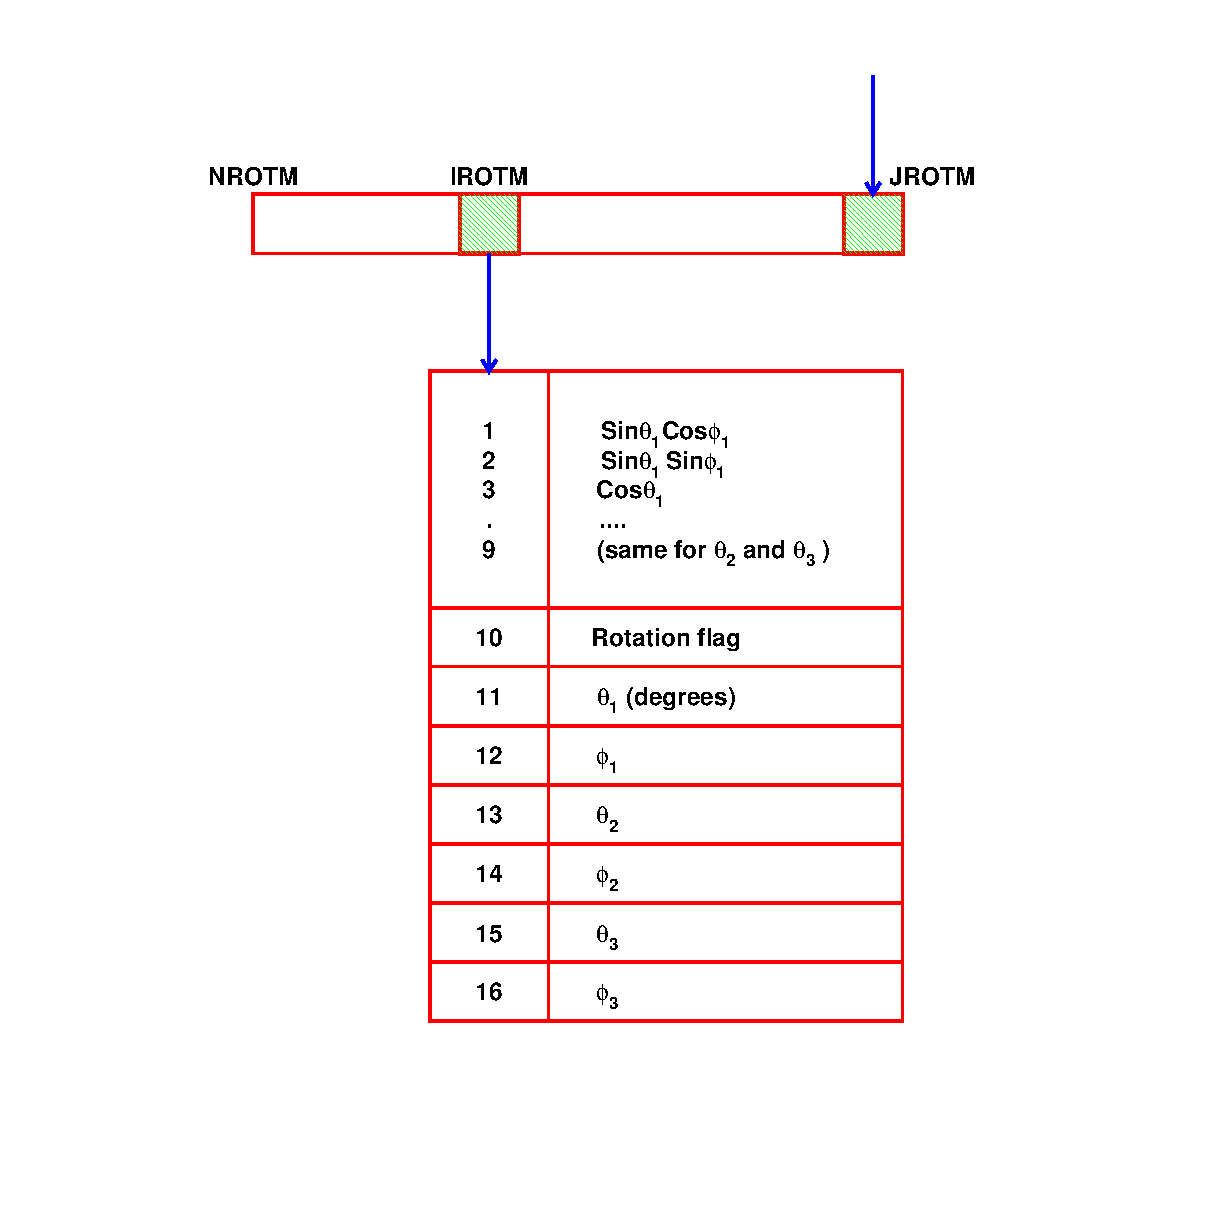
\epsfig{file=eps/geom299-1.eps,width=14cm}
     \caption{Layout of the {\tt JROTM} data structure}
     \label{fg:geom299-1}
\end{figure}

{\tt JR = LQ(JROTM-IROTM)} is the
pointer to the bank of the rotation matrix {\tt IROTM};
 
The rotation flag is computed by \Rind{GSROTM} to 
recognise simple rotation configurations. In particular it
is set to 0 for the unit matrix. 

%%%%%%%%%%%%%%%%%%%%%%%%%%%%%%%%%%%%%%%%%%%%%%%%%%%%%%%%%%%%%%%%%%%
%                                                                 %
%  GEANT manual in LaTeX form                              %
%                                                                 %
%  Michel Goossens (for translation into LaTeX)                   %
%  Version 1.00                                                   %
%  Last Mod. Jan 24 1991  1300   MG + IB                          %
%                                                                 %
%%%%%%%%%%%%%%%%%%%%%%%%%%%%%%%%%%%%%%%%%%%%%%%%%%%%%%%%%%%%%%%%%%%
\Origin{R.Brun, A.C.McPherson, F.Bruyant}
\Revision{S.Giani}
\Submitted{18.12.83}       \Revised{14.12.93}
\Version{Geant 3.16}       \Routid{GEOM300}

\Makehead{Finding in which volume a point is}

\Shubr{GMEDIA}{(X,NUMED*)}
\begin{DLtt}{MMMMMMMM}
\item[X] ({\tt REAL}) array of dimension 3 with the coordinates in the 
{\tt MRS};
\item[NUMED] ({\tt INTEGER}) medium number, if this is zero the point is 
outside the detector.
\end{DLtt}

Searches the geometrical tree structure to find in which volume the point 
{\tt X} is. The tracking medium is returned in {\tt NUMED}, and the common 
\FCind{/GCVOLU/} is updated.
 
\Rind{GMEDIA} uses the geometry data structure to conduct its search
starting its search from the last volume where a point was found.
If no previous search has been conducted, the first volume is used
as a starting point.

If the point is not inside the current volume, \Rind{GMEDIA} looks in its 
mother and so on, until it finds a volume which contains the point.
It then looks at the contents of this object and so on until the point 
is in a volume but in none of its contents (if any).

If this {\it downward} search terminates in a
{\tt 'MANY'} object, \Rind{GMEDIA} looks for another candidate. See
{\tt [GEOM110]} for a description of the {\tt `MANY'} volumes tratment.

The {\it physical} geometrical tree from the first volume
to the current one is stored in the common block \FCind{GCVOLU}
(see {\tt [BASE030]}) and in the structure {\tt JGPAR} (see {\tt [GEOM199]}).

\Shubr{GTMEDI}{(X,NUMED*)}
\begin{DLtt}{MMMMMMMM}
\item[X] ({\tt REAL}) array of dimension 3 with the coordinates in the 
{\tt MRS};
\item[NUMED] ({\tt INTEGER}) medium number, if this is zero the point is 
outside the detector.
\end{DLtt}

This routine performs the same function than \Rind{GMEDIA}, but it uses
the dynamical information of the particle history to speed-up the 
search:
\begin{itemize}
\item when {\tt INWVOL=2} (common \FCind{/GCTRAK/})
the particle just came out of a volume. In this
case, if {\tt INFROM} (common \FCind{/GCVOLU/}) is positive, it is
interpreted by \Rind{GTMEDI} as the number {\tt IN} of the content
just left, inside the mother volume
where the point {\tt X} is assumed to be. This content will not be
searched again.
\item the daughter of the current volume which limits the
geometrical step of the particle (i.e. where the particle would be heading
moving along a straight line) is searched first.
{\tt INGOTO} (common \FCind{/GCVOLU/}) is set by \Rind{GTNEXT}, to transmit 
the information
on this one volume which has limited the geometrical step {\tt SNEXT} as follows:
\begin{DLtt}{MMMM}
\item[$>$0] {\tt IN}$^{th}$ content;
\item[$=$0] current volume;
\item[$<$0] -{\tt NLONLY}, with {\tt NLONLY} defined as the lowest {\tt 'ONLY'}
level up in the tree which is an ancestor of the {\tt 'MANY'} volume 
where the point {\tt X} is.
\end{DLtt}
\end{itemize}

\Shubr{GINVOL}{(X,ISAME*)}
\begin{DLtt}{MMMMMMMM}
\item[X] ({\tt REAL}) array of dimension 3 with the coordinates in the 
{\tt MRS};
\item[ISAME] ({\tt INTEGER}) return flag.
\end{DLtt}
Checks if particle at point {\tt X} has left current volume.
If so, returns {\tt ISAME = 0} and prepares information useful to
identify the new volume entered, otherwise, returns {\tt ISAME = 1}.

%%%%%%%%%%%%%%%%%%%%%%%%%%%%%%%%%%%%%%%%%%%%%%%%%%%%%%%%%%%%%%%%%%%
%                                                                 %
%  GEANT manual in LaTeX form                                     %
%                                                                 %
%  Michel Goossens (for translation into LaTeX)                   %
%  Version 1.00                                                   %
%  Last Mod. Jan 24 1991  1300   MG + IB                          %
%                                                                 %
%%%%%%%%%%%%%%%%%%%%%%%%%%%%%%%%%%%%%%%%%%%%%%%%%%%%%%%%%%%%%%%%%%%
\Origin{R.Brun, A.C.McPherson}
\Revision{S.Giani}
\Submitted{01.06.83}             \Revised{15.12.93}
\Version{Geant 3.21}             \Routid{GEOM310}

\Makehead{Finding distance to next boundary}

\Shubr{GNEXT}{(X,SNEXT*,SAFETY*)}
\Shubr{GTNEXT}{(X,SNEXT*,SAFETY*)}
Finds distance to the next boundary.
It takes explicit account of shape content and uniqueness.
\begin{DLtt}{MMMMMMMM}
\item[X] ({\tt REAL}) array of 6 of coordinates and direction cosines;
\item[SNEXT] ({\tt REAL}) distance to the nearest volume boundary 
along the particle direction;
\item[SAFETY] ({\tt REAL}) {\it safety} distance, that is smaller distance
to any boundary;
\end{DLtt}
 
This routine evaluates the two {\it distances} which are needed by the
{\tt GEANT} tracking routines. \Rind{GTNEXT} and \Rind{GNEXT} perform
the same function, but \Rind{GNEXT} is a static routine which can be
called by the user, while \Rind{GTNEXT} is the routines used internally
by {\tt GEANT} during tracking, and it should not be called by the user.

If {\tt INFROM} (common \FCind{/GCVOLU/}) is different from 0, \Rind{GTNEXT}
interprets it as the daughter out of which the particle just came, and
uses the list of daughters stored with that volume, possibly modified by
\Rind{GSNEXT}/\Rind{GSNEAR} to calculate the distance to the next boundary.

The first action of \Rind{GTNEXT} is to calculate the {\tt SAFETY} distance.
If this is larger than the current step candidate, no other calculation is
performed and the {\tt IGNEXT} flag (common \FCind{/GCTRAK/}) is set to 0,
indicating that no change of volume is occurring at the end of the current
step. If the step is smaller than safety, then {\tt SNEXT} is computed.
If the step is smaller than {\tt SNEXT}, again there will not be any
change of volume during the step and {\tt IGNEXT} is set to 0.
If on the contrary the candidate step is larger than {\tt SNEXT}, a
change of volume will occur at the end of the step, and {\tt IGNEXT}
is set to 1 and {\tt INGOTO} (common \FCind{/GCTRAK/}) is set to the
number of the daughter where the particle is entering, if any.

Charged particles in magnetic field are transported with a similar logic.
However, even if the candidate step is smaller than {\tt SNEXT}, the
particle can still cross into another volume due to its bent path. When
tracking in magnetic field, after every step greater than {\tt SAFETY}
it is checked whether the particle is still in the same volume. If this is
not the case, the step is divided by two and transport is tried again.
Conversely a charged particle in magnetic field may still be in the
current volume even after having travelled the distance to the nearest
boundary along a {\it straight} line. So boundary crossing is declared
only when {\tt IGNEXT} is different from 0 and 
the difference between the real trajectory and the bent one is smaller
than {\tt EPSIL} (common \FCind{/GCTMED/}).


%%%%%%%%%%%%%%%%%%%%%%%%%%%%%%%%%%%%%%%%%%%%%%%%%%%%%%%%%%%%%%%%%%%
%                                                                 %
%  GEANT manual in LaTeX form                                     %
%                                                                 %
%  Version 1.00                                                   %
%                                                                 %
%  Last Mod.  9 June 1993  1300  MG                               %
%                                                                 %
%%%%%%%%%%%%%%%%%%%%%%%%%%%%%%%%%%%%%%%%%%%%%%%%%%%%%%%%%%%%%%%%%%%
\Origin{R. Brun}
\Submitted{18.08.87}         \Revised{15.12.93}
\Version{Geant 3.16}         \Routid{GEOM320}

\Makehead{Reference system transformations}
 
\Shubr{GMTOD}{(XM,XD*,IFLAG)}
\begin{DLtt}{MMMMMMMM}
\item[XM] ({\tt REAL}) array of 3 containing the input position
({\tt IFLAG=1}) or direction cosines ({\tt IFLAG=2}) in the {\tt M}aster
{\tt R}eference {\tt S}ystem;
\item[XD] ({\tt REAL}) array of 3 containing the output position
({\tt IFLAG=1}) or direction cosines ({\tt IFLAG=2}) in the 
(current) {\tt D}aughter {\tt R}eference {\tt S}ystem;
\item[IFLAG] ({\tt INTEGER}) transformation flag:
\begin{DLtt}{MMMM}
\item[1] input is a position, it must be translated and rotated;
\item[2] input is a direction, it must be rotated.
\end{DLtt}
\end{DLtt}

This routine transform coordinates or directions from the {\tt MRS}
to the reference system of the current volume. The
\FCind{/GCVOLU/} must be properly filled, either by the tracking
routines, by \Rind{GMEDIA} or by \Rind{GLVOLU}.

\Shubr{GDTOM}{(XD,XM*,IFLAG)}
Performs the inverse operation to \Rind{GMTOD}.

%%%%%%%%%%%%%%%%%%%%%%%%%%%%%%%%%%%%%%%%%%%%%%%%%%%%%%%%%%%%%%%%%%%
%                                                                 %
%  GEANT manual in LaTeX form                              %
%                                                                 %
%  Michel Goossens (for translation into LaTeX)                   %
%  Version 1.00                                                   %
%  Last Mod. Jan 24 1991  1300   MG + IB                          %
%                                                                 %
%%%%%%%%%%%%%%%%%%%%%%%%%%%%%%%%%%%%%%%%%%%%%%%%%%%%%%%%%%%%%%%%%%%
\Origin{R.Brun,F.Bruyant,A.C.McPherson}
\Revision{S.Egli}
\Submitted{16.12.83}          \Revised{15.12.93}
\Version{Geant 3.16}          \Routid{GEOM400}

\Makehead{Pseudo-division of a volume}

\Shubr{GSORD}{(CHNAME,ICORD)}
\begin{DLtt}{MMMMMMMM}
\item[CHNAME]  ({\tt CHARACTER*4}) name of the volume;
\item[ICORD]  ({\tt INTEGER}) direction of the pseudo-divisions:
\begin{DLtt}{MMMM}
\item[1] $x$;
\item[2] $y$;
\item[3] $z$;
\item[4] cylindrical $R$ ($\sqrt{x^2+y^2}$);
\item[5] spherical $\rho$ ($\sqrt{x^2+y^2+z^2}$);
\item[6] $\phi$, azimuthal angle;
\item[7] $\theta$, polar angle with respect to the $z$ axis.
\end{DLtt}
\end{DLtt}

This routine sets the search flag ({\tt Q(JVO+1)}) of volume {\tt CHNAME} 
to {\tt -ICORD}. When the definition of the geometry is complete and 
\Rind{GGCLOS} is called, this flag is interpreted as a request to order 
the content
of {\tt CHNAME} along {\it axis} {\tt ICORD}. This operation is 
performed by the routine \Rind{GGORD}.
\Rind{GGORD} computes the limits of each of the contents along the given
coordinate axis (see {\tt [GEOM001]}),
and prepares the lists of contents in each of the sections
defined by the neighbouring coordinate. The {\tt JVOLUM} structure 
is extended, for
the mother volume, with banks which contains the list of boundaries and the
lists of contents, so as to permit a binary search to access the contents
of interest. The coordinates are in the local system of the mother volume.
The routine \Rind{GGORD} will not be called if the number of contents 
exceeds 500.

The actual effect of this routine depends on the setting of the {\tt IOPTIM}
variable in the common \FCind{/GCOPTI/}. {\tt IOPTIM} is controlled by the
data record {\tt OPTI} or the interactive command with the same name.
The meaning of the different values of {\tt IOPTIM} is the following:
\begin{DLtt}{MMMM}
\item[$<$0] no call to \Rind{GGORD} will be made, irrespective of the
value of {\tt ISEARCH};
\item[~0] \Rind{GGORD} will be called for those volumes for which \Rind{GSORD}
has been called;
\item[~1] for all volumes with contents for which neither \Rind{GUSEAR} nor
\Rind{GSORD} has been called, the routine \Rind{GGORDQ} will be called;
\item[~2] \Rind{GGORDQ} is called for all volumes with contents
for which \Rind{GUSEAR} has not been called.
\end{DLtt}
 
\Rind{GGORDQ} orders the contents along all the possible axes and choses the
ordering which provides the lowest number of volumes per division.

%%%%%%%%%%%%%%%%%%%%%%%%%%%%%%%%%%%%%%%%%%%%%%%%%%%%%%%%%%%%%%%%%%%
%                                                                 %
%  GEANT manual in LaTeX form                              %
%                                                                 %
%  Michel Goossens (for translation into LaTeX)                   %
%  Version 1.00                                                   %
%  Last Mod. Jan 24 1991  1300   MG + IB                          %
%                                                                 %
%%%%%%%%%%%%%%%%%%%%%%%%%%%%%%%%%%%%%%%%%%%%%%%%%%%%%%%%%%%%%%%%%%%
\Origin{F.Bruyant, A.C.McPherson}
\Documentation{F.Carminati, M.Lefebvre}
\Submitted{16.12.83}                \Revised{14.12.93}
\Version{Geant 3.16}                \Routid{GEOM410}

\Makehead{Ordering the contents of a volume}

In the case of a mother volume containing a large number of daughters,
tracking can be rather slow. This is due to the fact that each time
{\tt GEANT} requires to know in which daughter it is or will be tracking,
it search through the whole list of daughter volumes.
This is done by {\tt GEANT} creating for every daughter volume a list
which contain pointers to all the daughters of the same mother.

Clearly this may be avoided, because at any step of tracking, the 
coordinates and direction cosines of the current step are known. From this
and the knowledge of the geometry, a restricted list of daughter volumes 
to be searched can be built. This can be accomplished in {\tt GEANT} in
two ways, which are described in this chapter.

{\bf Note}: the user must be aware that the following routines alter the
default search list of daughters of a given mother. A user mistake can
cause wrong transport because {\tt GEANT} does not make any check on the
correctness of the list of neighbours provided by the user.

\section*{Static ordering}
\Shubr{GSNEXT}{(CHMOTH,IN,NLIST,LIST)}
\begin{DLtt}{MMMMMMMM}
\item[CHMOTH] ({\tt CHARACTER*4}) name of the mother volume to be ordered;
\item[IN]     ({\tt INTEGER}) number of the content for which a list
is established;
\item[NLIST]  ({\tt INTEGER}) number of neighbours to be considered 
during tracking;
\item[LIST]  ({\tt INTEGER}) list of neighbours to volume {\tt IN}.
\end{DLtt}

This routine stores a given ordered {\tt LIST} of {\tt NLIST} daughter
volumes to search when leaving the {\tt IN}$^{th}$ daughter
of the mother volume {\tt CHMOTH}.

If {\tt IN=0}, for each content, \Rind{GSNEXT} builds a list limited to
the contents {\tt IN+1} (if it exists), {\tt IN-1} (if it exists) and 
{\tt IN} itself.

\Shubr{GSNEAR}{(CHMOTH,IN,NLIST,LIST)}
\begin{DLtt}{MMMMMMMM}
\item[CHMOTH] ({\tt CHARACTER*4}) name of the mother volume to be ordered;
\item[IN]     ({\tt INTEGER}) number of the content for which a list
is established;
\item[NLIST]  ({\tt INTEGER}) number of neighbours to be considered 
during tracking;
\item[LIST]  ({\tt INTEGER}) list of neighbours to volume {\tt IN}.
\end{DLtt}

This routine stores a given ordered {\tt LIST} of {\tt NLIST} daughter
volumes to search when leaving the {\tt IN}$^{th}$ daughter
of the mother volume {\tt CHMOTH}.
 
If {\tt LIST(1)}=0 the particle is back into the mother when leaving the
{\tt IN}$^{th}$ daughter. This means that the {\tt IN}$^{th}$ is not 
contiguous to any other daughter or to the boundary of the mother.

If {\tt IN}=-1, the mother does not have contents contiguous
to its boundaries (status bit 4 set in mother volume bank for action in
\Rind{GGCLOS}).

If {\tt IN}=0 for each content \Rind{GSNEAR} sets {\tt LIST(1)}=0.

\Rind{GSNEAR} must be called after all contents have been position ( except
when {\tt IN}=-1)

\section*{Dynamic ordering}

The list of neighbours to search when exiting from the {\tt IN}$^{th}$
content may depend also on the direction and position of the particle.
In case where it is necessary, for performance reasons, to exploit also
this information, {\tt GEANT} offers the possibility to the user to 
build a dynamic search list.

\Shubr{GSUNEA}{(CHNAME,ISEARC)}
\begin{DLtt}{MMMMMMMM}
\item[CHNAME] ({\tt CHARACTER*4}) name of the volume where the user search
has to be activated;
\item[ISEARCH] ({\tt INTEGER}) specifies the kind of search list to
be used: a positive value must be specified with this routine to activate
user search lists.
\end{DLtt}
This routine should be called once for every volume where user volume
search is activated.

\Shubr{GUNEAR}{(ISEARC,ICALL,XC,JNEAR)}
\begin{DLtt}{MMMMMMMM}
\item[ISEARCH] ({\tt INTEGER}) number associated to the volume in which
the user search is used, it is the same number set by the user with
\Rind{GSUNEA};
\item[ICALL] ({\tt INTEGER}) type of question that the list of volumes
must answer:
\begin{DLtt}{MMMM}
\item[1] \Rind{GMEDIA}-like call, where am I?
\item[2] \Rind{GTNEXT}-like call, where can I go?
\end{DLtt}
\item[XC] ({\tt REAL}) array of 6 containing the position and the
direction cosines of the particle ($x$, $y$, $z$, $p_x/p$, $p_y/p$, $p_x/p$);
\item[JNEAR] ({\tt INTEGER}) pointer to the volume list bank which has
to be filled by the user;
\end{DLtt}

The list of volumes where {\tt GEANT} has to search to answer the question
specified by {\tt ICALL} is returned by the user starting at {\tt Q(JNEAR+1}.
{\tt GEANT} will only look at the volumes specified by the user and in
the order in which they appear in the list. Daughters are numbered from 1
to N according to the order with which they have been positioned in the
mother. The list should be filled in the following way:

\begin{tabular}{lcp{7cm}}
{\tt IQ(JNEAR+1)} & = & {\tt N}, number of volumes in the list \\
{\tt IQ(JNEAR+1+1)} & = & number of the first daughter to search \\
{\tt IQ(JNEAR+1+2)} & = & number of the second daughter to search \\
.\\
.\\
.\\
{\tt IQ(JNEAR+1+N)} & = & number of the N$^{th}$ daughter to search 
\end{tabular}

The user should be aware that this routine is called very often, almost
at every tracking step, so it should be coded with the maximum efficiency
in mind.  An example of \Rind{GUNEAR} could be the following:

\begin{verbatim}
      SUBROUTINE GUNEAR(ISEARC,ICALL,XC,JNEAR)
*---              Make sure to add GEANT main store
+SEQ, GCBANK.
      DIMENSION XC(6), MYLIST(100)
*---              Executable code
      IF(ISEARC.EQ.1) THEN
*---              Build a list using XC and ISEARC for a GMEDIA type call
*---              Put all the daughters where the particle may be in
         MYLIST(1) = ....
         .
         .
         .
         MYLIST(N) = ....
      ELSE 
*---              Build a list using XC and ISEARC for a GTNEXT type call
*---              Put all the daughters where the particle may be going
         MYLIST(1) = ....
         .
         .
         .
         MYLIST(N) = ....
      ENDIF
*---              Return the information to GEANT
      DO 10 I=1,N
         IQ(JNEAR+1+I) = MYLIST(I)
  10  CONTINUE
      IQ(JNEAR+1) = N
*---              End of GUNEAR
      END
\end{verbatim}

%%%%%%%%%%%%%%%%%%%%%%%%%%%%%%%%%%%%%%%%%%%%%%%%%%%%%%%%%%%%%%%%%%%
%                                                                 %
%  GEANT manual in LaTeX form                              %
%                                                                 %
%  Michel Goossens (for translation into LaTeX)                   %
%  Version 1.00                                                   %
%  Last Mod. Jan 24 1991  1300   MG + IB                          %
%                                                                 %
%%%%%%%%%%%%%%%%%%%%%%%%%%%%%%%%%%%%%%%%%%%%%%%%%%%%%%%%%%%%%%%%%%%
\Origin{R.Brun, P.Zanarini}
\Submitted{15.08.83}           \Revised{15.12.93}
\Version{Geant 3.16}           \Routid{GEOM500}

\Makehead{Volume attributes}

\Shubr{GSATT}{(CHNAME,CHIATT,IVAL)}
 
\begin{DLtt}{MMMMMMMM}
\item [CHNAME] ({\tt CHARACTER*4}) volume name;
\item[CHIATT] ({\tt CHARACTER*4}) attribute to be set;
\item[IVAL] ({\tt INTEGER}) value to which the attribute is to be set.
\end{DLtt}

Changes the attribute {\tt CHIATT} of the volume called {\tt CHNAME} to the 
value {\tt IVAL}. The names and meaning of the attributes and their allowed
values are:
\begin{center}
\begin{tabular}{|ccl|}
\hline
Number & Name & \multicolumn{1}{c|}{Description} \\ \hline
1& {\tt WORK}
& \begin{tabular}{rp{5cm}}
0 & inactive volume \\
1 & active volume
\end{tabular} \\[3mm]
 & ~ &\\
2& {\tt SEEN} 
& \begin{tabular}{rp{5cm}}
-2 & only the volume is visible, but none of its descendants \\
-1 & the volume is not visible together with all its descendants \\
0 & the volume is not visible \\
1 & the volume is visible
\end{tabular} \\
 & ~ &\\
3&{\tt LSTY} & line style parameter (see {\tt [XINT002]}) \\

4&{\tt LWID} & line width parameter (see {\tt [DRAW400]}) \\

5&{\tt COLO} & area filling colour (see {\tt [XINT002]}) \\

6&{\tt FILL} & area filling resolution (see {\tt [DRAW400]}) \\

7&{\tt SET} & set number associated to the volume\\
8&{\tt DET} & detector number associated to the volume\\
9&{\tt DTYP} & detector type associated to the volume (1,2)\\
10&{\tt NODE} & dummy \\ \hline

\end{tabular} 
\end{center}

\Shubr{GFATT}{(CHNAME,CHIATT,IVAL*)}
Returns in {\tt IVAL} the attribute {\tt CHIATT} of the volume {\tt CHNAME}.
The arguments have the same meaning than for the routine \Rind{GSATT}.

\Shubr{GFPARA}{(CHNAME,NR,INTEXT,NPAR*,NATT*,PAR*,ATT*)}
\begin{DLtt}{MMMMMMMM}
\item[CHNAME]  ({\tt CHARACTER*4}) volume name;
\item[NR]      ({\tt INTEGER}) copy number;
\item[INTEXT] ({\tt INTEGER}) type of volume parameters requested:
\begin{DLtt}{MMMM}
\item[0] user parameters;
\item[1] internal parameters;
\end{DLtt}
\item[NPAR] ({\tt INTEGER}) number of parameters returned;
\item[NATT] ({\tt INTEGER}) number of attributes returned;
\item[PAR]  ({\tt REAL}) array of parameters;
\item[ATT] ({\tt REAL}) array of attributes.
\end{DLtt}
Returns parameters {\tt PAR(1...NPAR)} and
attributes {\tt ATT(1...NATT)} for the volume {\tt CHNAME} with copy number
{\tt NR}.

%%%%%%%%%%%%%%%%%%%%%%%%%%%%%%%%%%%%%%%%%%%%%%%%%%%%%%%%%%%%%%%%%%%
%                                                                 %
%  GEANT manual in LaTeX form                                     %
%                                                                 %
%  Michel Goossens (for translation into LaTeX)                   %
%  Version 1.00                                                   %
%  Last Mod. Jan 24 1991  1300   MG + IB                          %
%                                                                 %
%%%%%%%%%%%%%%%%%%%%%%%%%%%%%%%%%%%%%%%%%%%%%%%%%%%%%%%%%%%%%%%%%%%
\Origin{F.Bruyant, A.McPherson}
\Submitted{16.12.83}                \Revised{15.12.93}
\Version{Geant 3.16}                \Routid{GEOM600}
\Makehead{User initialisation of the common block /GCVOLU/}

\Shubr{GLVOLU}{(NLEV,LNAM,LNUM,IER*)}
\begin{DLtt}{MMMMMMM}
\item[NLEV] ({\tt INTEGER}) number of levels to fill;
\item[LNAM] ({\tt INTEGER}) array of {\tt NLEV} volume names stored
via the \Rind{UCTOH} routine;
\item[LNUM] ({\tt INTEGER}) array of {\tt NLEV} volume copy (or 
division) numbers;
\item[IER] ({\tt INTEGER}) returns code different from 0 in case of 
error, a diagnostic is also printed;
\end{DLtt}

This routine fills the volume parameters in common \FCind{/GCVOLU/}
for a physical tree, specified by the lists {\tt LNAM} and {\tt LNUM} of
volumes names and numbers, and for all its ascendants up to
level 1.

The routine is optimised and does not re-compute the part of
history already available in \FCind{GCVOLU}. This means that if
it is used in user programs outside the usual framework of the tracking,
the user has to initialise to zero {\tt NLEVEL} in common \FCind{GCVOLU}.

An example of use of \Rind{GLVOLU} in this context could be to find the
position and direction of a particle in the local coordinate system of
a volume:
\begin{verbatim}
      .
      .
+SEQ,GCVOLU
      DIMENSION LNAM(15), LNUM(15), POS(3), DIR(3), POSL(3), DIRL(3)
      .
      .
      CALL UCTOH('MOTH',LNAM(1),4,4)
      LNUM(1) = 1
      CALL UCTOH('CAL1',LNAM(2),4,4)
      LNUM(2) = 2
      CALL UCTOH('MOD1',LNAM(3),4,4)
      LNUM(3) = 5
      CALL UCTOH('CHAM',LNAM(4),4,4)
      LNUM(4) = 18
*---
      NLEVEL  = 0
      CALL GLVOLU(4,LNAM,LNUM,IER)
*---
      CALL GMTOD(POS,POSL,1)
      CALL GMTOD(DIR,DIRL,2)
      .
      .
\end{verbatim}

%%%%%%%%%%%%%%%%%%%%%%%%%%%%%%%%%%%%%%%%%%%%%%%%%%%%%%%%%%%%%%%%%%%
%                                                                 %
%  GEANT manual in LaTeX form                              %
%                                                                 %
%  Michel Goossens (for translation into LaTeX)                   %
%  Version 1.00                                                   %
%  Last Mod. Jan 24 1991  1300   MG + IB                          %
%                                                                 %
%%%%%%%%%%%%%%%%%%%%%%%%%%%%%%%%%%%%%%%%%%%%%%%%%%%%%%%%%%%%%%%%%%%
\Origin{R.Brun}
\Submitted{16.12.83}       \Revised{16.12.93}
\Version{Geant 3.16}       \Routid{GEOM700}
\Makehead{Medium search statistics}

In order to understand the behaviour and the performance of the 
geometry defined by the user, it is sometimes very useful to
accumulate the statistic of the various geometrical routines called.
This is done automatically by {\tt GEANT} if the statistical package
is activated via the data record {\tt STAT 1}. In this case the routine
\Rind{GBSTAT} is called by \Rind{GGCLOS}, \Rind{GFSTAT} is called by
the tracking routines \Rind{GINVOL}, \Rind{GTMEDI}, \Rind{GTNEXT},
\Rind{GTRACK} and \Rind{GMEDIA} to accumulate the statistics and \Rind{GPSTAT}
is called by \Rind{GLAST}.

\Shubr{GBSTAT}{}
Creates the data structure {\tt JGSTAT} in order to accumulate
statistics for the number of calls to routines
\Rind{GINVOL}, \Rind{GTMEDI}, \Rind{GTNEXT},
\Rind{GTRACK} and \Rind{GMEDIA}
and the total number of steps per volume.

\Shubr{GPSTAT}{}
Prints the volume statistics accumulated during the run. The
table which is printed is useful for optimizing the tracking
medium parameters associated to each volume.

\Shubr{GFSTAT}{}
Fills banks for volume statistics.
 
An example of output is the following:

\begin{center}
\tiny
\begin{verbatim}
              **************************************************************************************************************************
              *                                                                                                                        *
              *                                           V O L U M E    S T A T I S T I C S                                           *
              *                                                                                                                        *
              **************************************************************************************************************************
              *   VOLUME   *         GINVOL        *         GMEDIA        *         GTNEXT        *         GTMEDI        *  NSTEPS   *
              *    NAME    *   TOTAL   *   NLEVEL  *   TOTAL   *   NLEVEL  *   TOTAL   *   NLEVEL  *   TOTAL   *   NLEVEL  *  NLEVEL   *
              **************************************************************************************************************************
              *    CALO    *         0 *         0 *     43590 *         4 *    294743 *       250 *    246447 *       971 *       250 *
              *    CAL1    *         0 *         0 *     43056 *         0 *    284132 *         0 *    236482 *         0 *         0 *
              *    CAL2    *         0 *         0 *       524 *         0 *      9617 *         0 *      8283 *         0 *         0 *
              *    CAL3    *         0 *         0 *         0 *         0 *         9 *         0 *         8 *         0 *         0 *
              *    MOD1    *         0 *         0 *     43056 *        21 *    284132 *     42829 *    236482 *     42807 *     42848 *
              *    MOD2    *         0 *         0 *       524 *         0 *      9617 *      1570 *      8283 *      1570 *      1570 *
              *    MOD3    *         0 *         0 *         0 *         0 *         9 *         2 *         8 *         2 *         2 *
              *    SHIL    *         0 *         0 *      4935 *      4935 *     54736 *     54736 *     44480 *     44480 *     58247 *
              *    URPL    *         0 *         0 *     35932 *     35932 *     52803 *     52803 *     22571 *     22571 *     89953 *
              *    CHA1    *         0 *         0 *      1703 *         0 *     90507 *         0 *     86717 *         0 *         0 *
              *    TUB1    *         0 *         0 *      1703 *      1670 *     90507 *     62174 *     86717 *     58423 *     62700 *
              *    GAS1    *         0 *         0 *        33 *        33 *     28333 *     28333 *     28294 *     28294 *     28350 *
              *    EPO1    *         0 *         0 *       920 *       920 *     47007 *     47007 *     43032 *     43032 *     47742 *
              *    COPL    *         0 *         0 *         0 *         0 *         2 *         2 *         2 *         2 *         2 *
              *    CHA2    *         0 *         0 *        75 *         0 *      5037 *         0 *      4295 *         0 *         0 *
              *    TUB2    *         0 *         0 *        75 *        74 *      5037 *      4079 *      4295 *      3338 *      4159 *
              *    GAS2    *         0 *         0 *         1 *         1 *       958 *       958 *       957 *       957 *       958 *
              **************************************************************************************************************************
\end{verbatim}
\end{center}

%%%%%%%%%%%%%%%%%%%%%%%%%%%%%%%%%%%%%%%%%%%%%%%%%%%%%%%%%%%%%%%%%%%
%                                                                 %
%  GEANT manual in LaTeX form                              %
%                                                                 %
%  Michel Goossens (for translation into LaTeX)                   %
%  Version 1.00                                                   %
%  Last Mod. Jan 24 1991  1300   MG + IB                          %
%                                                                 %
%%%%%%%%%%%%%%%%%%%%%%%%%%%%%%%%%%%%%%%%%%%%%%%%%%%%%%%%%%%%%%%%%%%
\Origin{A.C.McPherson}
\Revision{F.Bruyant, R.Brun}   
\Submitted{16.12.83}         \Revised{16.12.93}
\Version{Geant 3.16}         \Routid{GEOM900}

\Makehead{End of geometry definition}
\Shubr{GGCLOS}{}
This routine should be called after all volumes, positions,
hits and digits have been defined. Its action is confined to
clean up the volume banks and to take any action required by the
ordering techniques. 

\Rind{GGCLOS} performs all the requested geometry optimisation, included
the creation of pseudo-divisions in volumes flagged by \Rind{GSORD}.
It performs the local development of tha last leaves of the
geometrical tree, where applicable.

It also calls the routine \Rind{GGDETV} which prepares the prototype lists of
volume names and maximum multiplicities which permit to identify uniquely
any sensitive detector whose generic name has been declared through the
routine \Rind{GSDETV} (and not \Rind{GSDET}) {\tt [HITS001]}.

\Rind{GGCLOS} must be called also after reading a geometry data structure
from disk.

%%%%%%%%%%%%%%%%%%%%%%%%%%%%%%%%%%%%%%%%%%%%%%%%%%%%%%%%%%%%%%%%%%%
%                                                                 %
%  GEANT manual in LaTeX form                              %
%                                                                 %
%  Michel Goossens (for translation into LaTeX)                   %
%  Version 1.00                                                   %
%  Last Mod. Jan 24 1991  1300   MG + IB                          %
%                                                                 %
%%%%%%%%%%%%%%%%%%%%%%%%%%%%%%%%%%%%%%%%%%%%%%%%%%%%%%%%%%%%%%%%%%%
 
 
 
 
\Origin{J.Vuoskoski, N. H\mbox{\o}imyr}
\Submitted{22.03.94}         \Revised{23.09.94}
\Version{Geant 3.21}         \Routid{GEOM910}
 
\Makehead{The CADINT Interface}
 
\section*{1 Introduction}
 
The engineering work in HEP for design,
analysis and manufacturing of detectors
requires Computer Aided Engineering (CAE) tools.
To ensure coherent design the same detector descriptions should
be used by physicists, engineers and, eventually, manufacturers. Efficient
exchange of data between CAE tools and
{\tt GEANT} becomes crucial.
 
 
The CADINT interface allows to export detector models from {\tt GEANT}
to Computer Aided Design (CAD) systems.
CADINT outputs detector models in the SET (Standard d'Echange
et de Transfert)~\cite{set} neutral file format.
A detector model is written as an assembly
of solid volumes, with respect to a global coordinate system. The geometric
representation used is
Constructed Solid Geometry (CSG)~\cite{mortenson}.
 
A {\tt GEANT} detector geometry exported through CADINT
into a CAD system can be used to
check the coherence of the model used in simulation.
The CADDFAS service at CERN can be used to convert SET files into IGES
(Initial Graphics Exchange Specification, an American
standard for exchange of CAD data)~\cite{iges} format, which is readable
by most CAD systems.
For more information about the CADDFAS service, send an e-mail to {\it
caddfas@cadd.cern.ch} with subject: {\it info}
 
 
 
 
 
\section*{2 SET File Format}
 
 
SET is a French standard
to exchange and archive CAD data.  It was developed as a neutral file format for
exchanging data between different CAD systems at Aerospatiale in 1983.
The aim was to develop
a more reliable alternative to IGES.  It became an official
French standard,
Afnor Z68-300, SET, in 1985.  SET was revised and extended in 1989.  The
version (89-06) used in CADINT, supports wireframe, surface and solid entities.
Entities for drafting and connectivity applications, as well as scientific
data and FEM (Finite Element Method) modelling are also included.
The philosophy behind the standard is that it should be able to
handle the complete information that may occur.
It is also considered to be important to have an unambiguously defined format,
that is compact in size,
and is flexible enough to handle future demands from the CAD/CAM industry.
 
 
The structure of SET is based upon a three level hierarchical structure,
which consists of data assemblies, data blocks, and data sub-blocks.
Information that is common to several blocks or assemblies, is stored in a
so-called dictionary.
 
\begin{itemize}
\item{\bf Assembly:} A SET data assembly is a collection of data defining
a certain piece of information, such as a mechanical part.
A SET file can contain one or more data assemblies;
 
\item{\bf Block:} In the nomenclature of the SET files,
the blocks are identified by an {\bf @},
followed by the number of the block identifying its type.
This number is followed by the block's reference number in the file.
(i.e. in a file with {\it n} blocks, the block sequence numbers will be from 0
 to {\it n}.)
After this, sub-blocks and dictionary entries used in the block follows.
A SET data block is an elementary entity, which consists of
definition or control data that are used in different applications.
Such entities could be geometric objects as points or lines, or other entities
like matrices, drawings and views or SET file identifiers;
 
 
\item{\bf Sub-block:} A sub-block consists of an identifier, and a list of data
that contributes to the description of the entity defined by the data block.
The different parameters inside a sub-block, such as coordinates, are
represented by their values. A sub-block has the identifier ``\#'', followed by
 its
type number, possible references to the dictionary, and parameters applicable in
the sub-block;
 
\item{\bf Dictionary:} The dictionary is a set of predefined parameters in the
specifications of the standard. They are accessible as dictionary entries which
are assigned an identifier (a colon ``{\bf :}'' and the dictionary number), and
 a
precise meaning given by authorised and/or default values.
 
\end{itemize}
 
References among entities in a SET file are made by using pointers,
either directly
from the blocks, or via sub-blocks or dictionary entries.  Pointers
to other blocks are identified by an ``{\bf !}'', followed by the sequence
numbers of the blocks.
SET has no unique mapping of  sub-block types and dictionary
entries into blocks. Several combinations are allowed for each different
block.  Definitions of possible combinations and guidelines for implementation
are given in the SET standard~\cite{set}.
 
 
 
\section*{3 Implementation}
 
 
In the CADINT interface,
a user can indicate a subtree of a detector by giving the name of a volume.
All the contents of this volume will be written into a SET file.
A user can also choose the contents by setting the daughter volumes
visible or invisible using the visibility attribute. Only the visible
volumes will be written into the SET file.
In order to avoid repeated volumes, a number of divisions can be chosen.
The rest of the divisions can be reproduced in a CAD system, if needed.
The colors of volumes defined by the {\tt GEANT} color attribute are
also transmitted into SET files.
 
 
The CADINT interface writes the geometry of a {\tt GEANT} detector model
in the SET file format in two basic phases:\\[-0.7cm]
 
\begin{enumerate}
\item write the volume information;\\[-0.7cm]
\item write the position information.\\[-0.5cm]
\end{enumerate}
 
The interface writes volumes into the SET format as
CSG solids i.e. the volumes are created using extrusions, revolutions,
ruled solids, rectangular parallelepipeds, etc.
Divisions are written as normal volumes.
Every division of a divided volume is
a distinct volume in a SET file. An index is attached to the end
of the name of each of
the divisions in order to distinguish each division instance.
The indexing of instances is reset in each division.
An index is attached to the end of the volume name of multiple copies
of normal volumes as well.
 
In SET format, a volume must be first written, after that it can
be positioned. All volumes are positioned with respect to
the global coordinate system. Thus, the tree structure
in the SET file is flat. There will be overlaps between volumes,
since no Boolean operations
are used to define the tree structure. However, the tree structure
is written into a separate file. The material information
is written into this same text file.
 
The interface  decodes the {\tt JVOLUM} data structure and
computes the necessary parameters if needed (negative parameters,
dimensions of divisions, etc.).
These computations are based on the {\tt GEANT} drawing routines.
The interface decodes a detector model starting from the global
mother volume. After that it decodes the first daughter volume in the
left side of the tree. The daughter volume can be a normal volume or a division.
It continues decoding daughter volumes until it
is at the bottom of the tree. After that the interface
returns one level and decodes the next daughter of the current volume
if any exists. In a case of a divided volume, the divisions are treated
in the same way as the daughter volumes.
The creation of the SET file is performed simultaneously.
 
 
\subsection*{3.1 Volume Information}
 
 
The tree decoding routine transfers the volume information
during decoding to the relevant
shape routine which writes the volumes into the SET file.
Every different shape has its own routine.
For example, the simplest shape, {\tt BOX}, is written
in the  SET format as follows:
 
\noindent{\tt@50,N1,:5,2\#60,X,Y,Z\\
@302,N2\#317,-DX,-DY,-DZ\\
@100,N3,:5,2,:9,'Name'\#101,!N1,!N2}\\
 
\newpage
 
\noindent Where\\[-0.7cm]
\begin{itemize}
\item {\bf{\tt @50}} is the block number which defines a primitive
 solid;\\[-0.7cm]
\item {\bf{\tt N1,N2,N3}} are the sequence numbers of each block;\\[-0.7cm]
\item {\bf{\tt :5,2}}  is the dictionary entry number which gives a total
subordination to one block;\\[-0.7cm]
\item {\bf{\tt \#60}} is the sub-block number which defines the geometric
parameters of a solid rectangular parallelepiped;\\[-0.7cm]
\item {\bf{\tt X,Y,Z}} are the dimensions of the rectangular
 parallelepiped;\\[-0.7cm]
\item {\bf{\tt @302}} is the block number for geometric
 transformation;\\[-0.7cm]
\item {\bf{\tt \#317}} is the sub-block number for translation;\\[-0.7cm]
\item {\bf{\tt DX,DY,DZ}} are the coefficients of the translation;\\[-0.7cm]
\item {\bf{\tt @100}} is the block number which defines a constructed
 solid;\\[-0.7cm]
\item {\bf{\tt :9}}  is the dictionary entry number for a name associated
with the block;\\[-0.7cm]
\item {\bf \tt Name} is the name of the volume;\\[-0.7cm]
\item {\bf{\tt \#101}} is the sub-block number for transformation
 operation.\\[-0.5cm]
\end{itemize}
 
The rectangular parallelepiped is first defined with the given parameters.
Then the translation of coordinates is defined. The translation is necessary
since {\tt GEANT} and SET use origins in different places. Finally,
the transformation operation is defined for a constructed solid which
in this case is the translation of the coordinates of a primitive solid.
The GEANT shapes are converted to SET as follows:
 
\begin{center}
 \begin{tabular}{|l|p{9.0 cm}|}
 \hline
 \bf SHAPE           &  \bf DEFINITION IN SET \\
 \hline
BOX  &   rectangular parallelepiped \\
TRD1 &   ruled solid between 2 faces   \\
TRD2 &   ruled solid between 2 faces \\
TRAP &   ruled solid between 2 faces \\
TUBE &   solid of revolution of a face \\
TUBS &   solid of revolution of a face \\
CONE &   solid of revolution of a face \\
CONS &   solid of revolution of a face \\
SPHE &   sphere \\
PARA &   ruled solid between 2 faces \\
PGON &   first segment ruled solid, other segments copied and rotated,
         finally boolean union for all the segments \\
PCON &   solid of revolution of a face \\
ELTU &   solid of linear extrusion of a face \\
HYPE &   not implemented \\
GTRA &   ruled solid between 2 faces \\
CTUB &   solid of revolution and boolean subtraction by 2 half-spaces \\
 \hline
 \end{tabular}
\end{center}
 
 
\subsection*{3.2 Position Information}
 
The position information of
a volume is handled by a routine,
which writes the coordinates and the rotation matrix. The tree decoding
routine transforms the coordinates and the rotation matrix of a volume 
to the global coordinate system, and then transfers the data
to the routine which writes the translation and rotation of a volume into
the SET format as follows:
 
\noindent{\tt @302,N1\#301,M1,M2,M3,M4,M5,M6,M7,M8,M9,XC,YC,ZC\\
@100,N2,:9,'Name'\#101,!N1(of the shape),!N1}\\
 
\newpage
 
\noindent Where\\[-0.7cm]
\begin{itemize}
\item {\bf{\tt @302}} is the block number for geometric
 transformation;\\[-0.7cm]
\item {\bf{\tt N1,N2}} are the sequence numbers of each block;\\[-0.7cm]
\item {\bf{\tt \#301}} is the sub-block number which defines the coefficients
of the rotation-translation matrix;\\[-0.7cm]
\item {\bf{\tt M1...M9}} are the  coefficients of the rotation matrix;\\[-0.7cm]
\item {\bf{\tt XC,YC,ZC}} are the components of the translation
 vector;\\[-0.7cm]
\item {\bf{\tt @100}} is the block number which defines a constructed
 solid;\\[-0.7cm]
\item {\bf{\tt :9}}  is the dictionary entry number for a name associated
with the block;\\[-0.7cm]
\item {\bf{\tt Name}} is the name of the volume;\\[-0.7cm]
\item {\bf{\tt \#101}} is the sub-block number for transformation
 operation;\\[-0.7cm]
\item {\bf{\tt !N1}} is the reference to sequence number of the mother
volume.\\[-0.5cm]
\end{itemize}
 
The geometric transformation is first defined with the given parameters
and then the transformation operation is defined for a constructed solid.
The principle of writing divisions into the SET format is
equivalent to the case of normal volumes.
 
\subsection*{3.3 Material and Tree Information}
 
The material file is written into a separate file simultaneously with the
SET file. It contains information on tracking medium, material and density for
each defined volume. The {\tt GEANT} tree is written into this same file. After
 the
volume name there follows the number of daughters and daughter names.
In a case of divided volume, the negative number of divisions is given after
the name of the divided volume, and followed by the offset, step
and the name of the division instance.
An output of a material file of a {\tt GEANT} example program:
 
\footnotesize{
\begin{verbatim}
 GEANT-SET MATERIAL LISTING FILE
 --------------------------------
 Materials in the geometry described in
 the .SET file:  gexam4.set
 
Volume name  Tracking media   Material         Density
 
CALO         1 AIR            1 AIR            0.12000001E-02
CAL1         1 AIR            1 AIR            0.12000001E-02
MOD1         1 AIR            1 AIR            0.12000001E-02
CAL2         1 AIR            1 AIR            0.12000001E-02
MOD2         1 AIR            1 AIR            0.12000001E-02
CAL3         1 AIR            1 AIR            0.12000001E-02
MOD3         1 AIR            1 AIR            0.12000001E-02
EPO1         4 CARBON         4 CARBON         0.22650001E+01
CHA1         6 BRASS          6 BRASS          0.85600004E+01
TUB1         6 BRASS          6 BRASS          0.85600004E+01
GAS1         5 GAS            5 ARG/ISOBU      0.21360000E-02
 
 GEANT TREE
 ----------
  The GEANT tree starting from the given volume
 
CALO    6  CAL1  CAL2  CAL3  EPO1  CHA1  EPO1
CAL1  -64  -0.48000000E+02   0.15000000E+01  MOD1
CAL2  -35  -0.43750000E+02   0.25000000E+01  MOD2
CAL3  -13  -0.24050001E+02   0.37000003E+01  MOD3
CHA1  -40  -0.25000000E+02   0.12500000E+01  TUB1
MOD1    6  SHIL  URPL  SHIL  EPO1  CHA1  EPO1
MOD2    4  SHIL  URPL  SHIL  CHA2
MOD3    2  COPL  CHA2
TUB1    1  GAS1
CHA2  -72  -0.23500000E+02   0.65277779E+00  TUB2
TUB2    1  GAS2
 
        ------ end of file -------
\end{verbatim}
}
\normalsize
 
\section*{4 Usage}
 
 
 
In order to carry out a successful transfer of a detector model,
a user needs to be
aware of certain limitations of the interface. The user is recommended
to communicate
with the engineers using CAD systems to establish a proper transfer methodology.
If a CAD system is not capable of receiving the whole detector geometry
in a single SET file, a user can transfer a detector model in smaller parts.
These parts can then be joined together in the CAD system.
Normally it is a good idea to just export one instance of each division
in order to limit the number of exported volumes.
The divisions can be reproduced in CAD systems.
It is impossible to give an exact size-limit for a detector model
which can be transferred in one file, because the limitation
depends on the structure of the detector model.
 
 
The {\tt GEANT} graphics package  provides excellent capabilities for
viewing parts of a detector model which is to be exported. Using
the visibility attribute and the number of division instances, a
user will be able to see what is to be exported. A user can use different
colors in order to help to distinguish different volumes (eg division
instances, etc.) in a CAD system.
Dummy volumes, such as mothers made of air or vacuum should be suppressed using
the visibility attribute, since the interface is currently not able to discard
such information.
A user must remember to specify the drawing parameters again if he
wants to draw the detector model after using the interface.
This is because the interface uses modified drawing routines.
 
A plot of the {\tt GEANT} tree can be useful for engineers to understand the
structure of the {\tt GEANT} detector model. {\tt GEANT}
volume names are useful references
regarding the material and tree information. The tree information is also
provided in the material file, but a graphical presentation is often useful.
 
 
 
 
 
\begin{thebibliography}{99}
 
 
 
 
\bibitem{set} French Standardization, Data exchange and transfer
standard specification, Afnor 1989.
 
 
\bibitem{mortenson} Michael E. Mortenson, Geometric Modeling, John
Wiley \& Sons, Inc., 1985.
 
 
 
\bibitem{iges} US department of Commerce, Initial Graphics Exchange
Specification, 1988.
 
 
 
\end{thebibliography}
 
 
 
 
 
 

\putbib[cnasbibl,geabibl]
\end{bibunit}
 
%%     HITS part     %%
 
\begin{bibunit}[unsrt]
\renewcommand{\bibname}{HITS Bibliography}
%%%%%%%%%%%%%%%%%%%%%%%%%%%%%%%%%%%%%%%%%%%%%%%%%%%%%%%%%%%%%%%%%%%
%                                                                 %
%  GEANT manual in LaTeX form                              %
%                                                                 %
%  Michel Goossens (for translation into LaTeX)                   %
%  Version 1.00                                                   %
%  Last Mod. Jan 24 1991  1300   MG + IB                          %
%                                                                 %
%%%%%%%%%%%%%%%%%%%%%%%%%%%%%%%%%%%%%%%%%%%%%%%%%%%%%%%%%%%%%%%%%%%
\Documentation{F.Bruyant}
\Submitted{15.08.84}         \Revised{17.12.93}
\Version{Geant 3.16}         \Routid{HITS001}
\Makehead{The detector response package}
\section{Introduction}
In the context of {\tt GEANT}:
\begin{itemize}
\item {\bf hit} is the user-defined {\it information} recorded at 
tracking time to keep track of the interaction between one
particle and a given detector,
and necessary to compute the digitisations later.
\item  {\bf digitisation} ({\it digit}) is the user-defined
{\tt information} simulating the response
of a given detector element, usually estimated
after tracking a complete event.
\end{itemize}
The detector response package consists of tools to store,
retrieve or print the information relevant to hits and
digitisation which is in the data structures
{\tt JSET, JHITS} and {\tt JDIGI}.
A few subroutines which may
help the user to solve some of the usual digitisation problems
in simple detectors
have been added to the package, e.g. the intersection of a
track with a plane or a cylinder
and the digitisation of conventional drift and {\tt MWP} chambers.

For complex setups with different types of detectors
the user has normally to define
several types of hits and digitisations.
In addition to the hits generated by all particles of the
current event, computing the digitisations
requires usually some information about the intrinsic
characteristics and performance of the detectors.
The information to be recorded for the hits and digitisations
is highly experiment dependent, therefore only a framework
can be proposed to store it.
 
Two remarks can be made:
\begin{itemize}
\item during the life of an experiment, 
the stability of the format and content of the information to be stored
is usually reached much earlier for the hits than for the digitisations.
Therefore the user may save computing time
by designing an intermediate event output at the hits level.
\item  the scheme proposed for storing the digitisations
should in any case be considered as
an intermediate stage, a further processing of the data being necessary
if the user wants to
simulate more closely the specific format of the real
data-acquisition system.
\end{itemize}

\section{{\tt SET}s and {\tt DET}ectors}

The reader is assumed to be familiar with the way the
geometrical setup is described ({\tt [GEOM]}), in particular
with the concepts of logical and physical volume tree structure.

The user is required to classify into sets all sensitive detectors
(defined as those volume defined as detector via \Rind{GSDET}/\Rind{GSDETV})
for which he wants to store hits in the data structure {\tt JHITS}.
The 4-character names which identify the sets are user defined,
and the list of sets
which the user wants to activate for a given run can be entered
through the data record {\tt SETS}.
The user can group together in one or in several sets
detectors of the same or different types. For convenience,
it is recommended to have at least one set for
each main component of the setup, e.g. hadronic calorimeters,
electromagnetic calorimeters, vertex chamber, etc.

A volume can be declared as a sensitive detector through the tracking
medium parameter {\tt ISVOL},
and allocated to a set through the subroutine \Rind{GSDET} or
\Rind{GSDETV}.
Each (logical) sensitive detector is identified by the 4-character
name of the corresponding volume. As a given volume
may describe several similar detectors in the physical setup,
some additional information is needed for associating
correctly the hits with the physical detectors.

When using \Rind{GSDET} the user has to enter the (shortest) list of volume
{\bf names} (the vector {\tt CHNMSV}), which permits unambiguous
identification of the path through the physical tree,
even in the presence of multiple copies.
This identification is obtained by specifying a list of volume
{\bf numbers} (the vector {\tt NUMBV}), in a one to one
correspondence with the list of volume names.
This list, after packing, will constitute the
identifier of the physical detector.

If \Rind{GSDETV} is used instead of
\Rind{GSDET} then the routine
\Rind{GGDETV} (called by \Rind{GGCLOS}) constructs the lists
{\tt CHNMSV} automatically and stores them in the structure {\tt JSET}.

\section{The user tools}
 
The data structure {\tt JSET} is built through
calls to the routine  \Rind{GSDET} or \Rind{GSDETV}
which assign detectors to
sets and define their parameters. After this, the
following routines can be called, for each detector, to complete the structure:
\begin{DLtt}{MMMMMMMM}
\item[\Rind{GSDETH}] provides the parameters required for the storage of the
hit elements in the data structure {\tt JHITS},
such as the packing and scaling conventions;
\item[\Rind{GSDETD}] provides the parameters required for the storage of
the digitisations in the structure {\tt JDIGI},
such as the packing conventions;
\item[\Rind{GSDETU}] adds the user parameters, which may consist,
for instance, of the intrinsic detector
characteristics needed for computing the digitisations.
\end{DLtt}

To permit storage of more than one type of hit for a given sensitive
detector, or to provide additional detector entries,
detector {\it aliases} can be defined through calls to the routine
\Rind{GSDETA}. They are entered in the {\tt JSET} structure as new detectors,
with the same geometrical characteristics as the original one.
The user has the possibility to call appropriate routines
\Rind{GSDETH}, \Rind{GSDETD} and \Rind{GSDETU} for this new detector.

During the tracking, for each step inside the
sensitive detectors, under control of the subroutine
\Rind{GUSTEP}, the hits can be stored in the data structure
{\tt JHITS} through the subroutine \Rind{GSAHIT} (or \Rind{GSCHIT}, more
appropriate for calorimetry).
For each hit the information consists of:
\begin{itemize}
\item the reference to the track in the structure {\tt JKINE};
\item the packed identifier of the physical detector;
\item the packed data for the different elements of the hit.
\end{itemize}

When the tracking has been completed for the whole
event the digitisations can be
computed in the user subroutine \Rind{GUDIGI} which
may extract the hits with the subroutine \Rind{GFHITS} and
store the digitisations in the data structure {\tt JDIGI}, with
the subroutine \Rind{GSDIGI}.
For each digitisation the information should at least consist of:
\begin{itemize}
\item the reference to the track(s);
\item the packed identifier of the physical detector;
\item the packed data for the digitisation itself.
\end{itemize}

\section{Retrieval of geometrical information}
 
The packed identifier of a physical detector, stored as part of the hit
(or digitisation) information, is returned unpacked by the routine
\Rind{GFHITS} (or \Rind{GFDIGI}) which extracts the
information from the {\tt JHITS} or {\tt JDIGI} structures,
and may be used to retrieve the geometrical characteristics
of the given detector.

If the detectors have been defined by the routine \Rind{GSDETV}, the
geometrical information can be retrieved by the routines \Rind{GFPATH}
and \Rind{GLVOLU}. \Rind{GFPATH} prepares the lists {\tt CHNAM} and {\tt LNUM} 
required by \Rind{GLVOLU} ({\tt [GEOM001]}), from the information
preprocessed at initialisation time by the routine \Rind{GGDETV} and
stored in the structure {\tt JSET}

%%%%%%%%%%%%%%%%%%%%%%%%%%%%%%%%%%%%%%%%%%%%%%%%%%%%%%%%%%%%%%%%%%%
%                                                                 %
%  GEANT manual in LaTeX form                              %
%                                                                 %
%  Michel Goossens (for translation into LaTeX)                   %
%  Version 1.00                                                   %
%  Last Mod. Jan 24 1991  1300   MG + IB                          %
%                                                                 %
%%%%%%%%%%%%%%%%%%%%%%%%%%%%%%%%%%%%%%%%%%%%%%%%%%%%%%%%%%%%%%%%%%%
\Origin{R.Brun,F.Bruyant}
\Submitted{01.11.83}                \Revised{17.12.93}
\Version{Geant 3.16}                \Routid{HITS100}
\Makehead{Sensitive DETector definition}
\Shubr{GSDET}{(CHSET,CHDET,NV,CHNMSV,NBITSV,IDTYP,NWHI,NWDI,ISET*,IDET*)}
 
\begin{DLtt}{MMMMMMMM}
\item[CHSET] ({\tt CHARACTER*4}) set identifier, user defined;
\item[CHDET] ({\tt CHARACTER*4}) detector identifier,
has to be the name of an existing volume;
\item[NV] ({\tt INTEGER}) number of volume descriptors;
\item[CHNMSV] ({\tt CHARACTER*4}) array of {\tt NV} volume descriptors;
\item[NBITSV] ({\tt INTEGER}) array of {\tt NV}, {\tt NBITSV(I)} 
({\tt I=1,...,NV}) is the number of bits in which to pack the copy 
number of volume {\tt CHNMSV(I)};
\item[IDTYP] ({\tt INTEGER}) detector type, user defined;
\item[NWHI] ({\tt INTEGER}) initial size of {\tt HITS} banks;
\item[NWDI] ({\tt INTEGER}) initial size of {\tt DIGI} banks;
\item[ISET] ({\tt INTEGER}) position of set in bank {\tt JSET};
\item[IDET] ({\tt INTEGER}) position of detector in bank {\tt JS=LQ(JSET-ISET)}.
\end{DLtt}

Assigns detector {\tt CHDET} to the set {\tt CHSET}
and defines its basic parameters.
 
{\bf Note:} The vector {\tt CHNMSV} (length {\tt NV)} contains the list of
volume names which permit unambiguous identification of all copies of
volume {\tt CHDET} [see example in {\tt [HITS110]}.
Each element of the vector {\tt NBITSV} (length {\tt NV}) is the number
of bits used for packing the number of the corresponding volume, when building
the packed identifier of a given physical detector.

For more details see the example given in {\tt [HITS110]}.
The detector type {\tt IDTYP} is not used internally by {\tt GEANT}
and can be used to distinguish quickly between various
kinds of detectors, in the routine \Rind{GUSTEP} for example.

\Shubr{GSDETV}{(CHSET,CHDET,IDTYP,NWHI,NWDI,ISET*,IDET*)}
The arguments of this routine are the same than the previous one,
but {\tt NAMES, NBITSV} will be computed by \Rind{GGDETV} called by
\Rind{GGCLOS}) (see {\tt [HITS001]}).

\Shubr{GFDET}{(CHSET,CHDET,NV*,CHNMSV*,NBITSV*,IDTYP*,NWHI*,NWDI*,ISET*,IDET*)}
Returns the parameters for detector {\tt CHDET} of set {\tt CHSET}, the
arguments have the same meaning than for routine \Rind{GSDET}.

\Shubr{GPSETS}{(CHSET,CHDET)}
Prints {\tt SET} and {\tt DET}ector parameters.
\begin{DLtt}{MMMMMMMM}
\item[CHSET] ({\tt CHARACTER*4}) set to be printed, if {\tt *} prints 
all detectors of all sets;
\item[CHDET] ({\tt CHARACTER*4}) detector to be printed, if {\tt *} prints
all detectors of set {\tt CHSET}.
\end{DLtt}
 

%%%%%%%%%%%%%%%%%%%%%%%%%%%%%%%%%%%%%%%%%%%%%%%%%%%%%%%%%%%%%%%%%%%
%                                                                 %
%  GEANT manual in LaTeX form                              %
%                                                                 %
%  Michel Goossens (for translation into LaTeX)                   %
%  Version 1.00                                                   %
%  Last Mod. Jan 24 1991  1300   MG + IB                          %
%                                                                 %
%%%%%%%%%%%%%%%%%%%%%%%%%%%%%%%%%%%%%%%%%%%%%%%%%%%%%%%%%%%%%%%%%%%
\Origin{F.Bruyant}
\Submitted{13.06. 85}      \Revised{16.12.93}
\Version{Geant 3.16}       \Routid{HITS105}

\Makehead{Detector aliases}
Detector {\tt aliases} can be specified for any sensitive detector for which
the user either needs to store more than one type of hit
or wants to define additional detector entries.

\Shubr{GSDETA}{(CHSET,CHDET,CHALI,NWHI,NWDI,IALI*)}
\begin{DLtt}{MMMMMMMM}
\item[CHSET] ({\tt CHARACTER*4}) set name;
\item[CHDET] ({\tt CHARACTER*4}) name of the detector for which an alias
is being defined;
\item[CHALI] ({\tt CHARACTER*4}) alias name;
\item[NWHI] ({\tt INTEGER}) initial number of words of {\tt HITS} banks;
\item[NWDI] ({\tt INTEGER}) initial number of words of {\tt DIGI} banks;
\item[IALI] ({\tt INTEGER}) position of alias in bank {\tt JS=LQ(JSET-ISET)}.
\end{DLtt}

Defines an alias {\tt CHALI} for detector {\tt CHDET} of set {\tt CHSET} and
enters it in the {\tt JSET} structure as an additional detector in the
corresponding set, at the position {\tt IALI}. The new detector will be
a copy at position {\tt IALI} of the original detector
{\tt CHDET}, with empty links to the \Rind{GSDETH}, \Rind{GSDETD} and
\Rind{GSDETU} parameter banks.
The user can therefore call these three routines again with the
arguments appropriate to the detector {\tt CHALI}.
Several aliases can be defined for
the same detector through calls to \Rind{GSDETA}.

%%%%%%%%%%%%%%%%%%%%%%%%%%%%%%%%%%%%%%%%%%%%%%%%%%%%%%%%%%%%%%%%%%%
%                                                                 %
%  GEANT manual in LaTeX form                                     %
%                                                                 %
%  Michel Goossens (for translation into LaTeX)                   %
%  Version 1.00                                                   %
%  Last Mod. Jan 24 1991  1300   MG + IB                          %
%                                                                 %
%%%%%%%%%%%%%%%%%%%%%%%%%%%%%%%%%%%%%%%%%%%%%%%%%%%%%%%%%%%%%%%%%%%
\Origin{R.Brun}
\Submitted{01.11.83}     \Revised{17.12.93}
\Version{Geant 3.16}     \Routid{HITS110}

\Makehead{DETector hit parameters}

\Shubr{GSDETH}{(CHSET,CHDET,NH,CHNAMH,NBITSH,ORIG,FACT)}
\begin{DLtt}{MMMMMMMM}
\item[CHSET] ({\tt CHARACTER*4}) set name;
\item[CHDET] ({\tt CHARACTER*4}) detector name;
\item[NH] ({\tt INTEGER}) number of the components of a hit;
\item[CHNAMH] ({\tt CHARACTER*4}) array of {\tt NH} names for the hit components;
\item[NBITSH] ({\tt INTEGER}) array of {\tt NH}, 
{\tt NBITSH(I)} ({\tt I=1,...NH}) is the number of bits in which to pack
the {\tt I$^{th}$} component of the hit;
\item[ORIG] ({\tt REAL}) array of {\tt NH} offset applied before packing
the hits values;
\item[FACT] ({\tt REAL}) array of {\tt NH} scale factors applied before packing
the hits values;
\end{DLtt}

Defines hit parameters for detector {\tt CHDET} of set {\tt CHSET}.
The routine must be called at initialisation time once the
geometrical volumes have been defined to describe
the hit elements and the way to pack them in the data structure {\tt JHITS}.
The value of the hit before packing is transformed in the following way:

\begin{center}
\tt VAL(I) = (HIT(I)+ORIG(I)) $\times$ FACT(I)
\end{center}

\section*{Example}

Assume an electromagnetic calorimeter {\tt ECAL} divided into
40 {\tt PHI} sections called {\tt EPHI}. Each {\tt EPHI} division is in turn
divided along the $z$ axis in 60 sections called {\tt EZRI}. Each {\tt EZRI}
is finally divided into 4 lead glass blocks called {\tt BLOC}.
The geometrical information to describe one hit will then be:

\begin{itemize}
\item the {\tt EPHI} section number (between 1 and 40);
\item the {\tt EZRI} division number (between 1 and 60);
\item the {\tt BLOC} number (1 to 4).
\end{itemize}

The quantities which should be stored for each hit are:
 
\begin{DLtt}{MMMM}
\item[X] $x$ position of the hit in the lead glass block ($-1000<x<1000$);
\item[Y] $y$ position of the hit in the lead glass block ($-1000<y<1000$);
\item[Z] $z$ position of the hit in the lead glass block ($-1000<z<1000$);
\item[E]energy of the particle;
\item[ELOS]the energy deposited;
\end{DLtt}

In this scheme a hit could look like:

\begin{center}
\begin{tabular}{l@{\hspace{2cm}}l}
Element & Value \\ \hline
\tt EPHI  &  12  \\
\tt EZRI  &  41  \\
\tt BLOC  &   3  \\
\tt X  &     7.89 cm  \\
\tt Y  &     -345.6 cm  \\
\tt Z  &     1234.8 cm  \\
\tt E  &     12 Gev  \\
\tt ELOS  &   11.85 Gev  \\
\end{tabular}
\end{center}

The code to define the {\tt SET/DET/HIT} information could be:
\begin{verbatim}
      CHARACTER*4 CHNMSV(3),CHNAMH(5)
      DIMENSION   NBITSV(3),NBITSH(5)
      DIMENSION   ORIG(5),FACT(5)
*---
      DATA CHNMSV/'EPHI','EZRI','BLOC'/
      DATA NBITSV/     6,     6,     3/
*---
      DATA CHNAMH /'X   ','Y   ','Z   ','E   ','ELOS'/
      DATA NBITSH /    16,    16,    16,    16,    16/
      DATA ORIG   / 1000., 1000., 1000.,    0.,    0./
      DATA FACT   /   10.,   10.,   10.,  100.,  100./
*---
      CALL GSDET ('ECAL','BLOC',3,CHNMSV,NBITSV,2,100,100,ISET,IDET)
      CALL GSDETH('ECAL','BLOC',5,CHNAMH,NBITSH,ORIG,FACT)
\end{verbatim}

\Shubr{GFDETH}{(CHSET,CHDET,NH*,CHNAMH*,NBITSH*,ORIG*,FACT*)}
Returns the hit parameters for detector {\tt CHDET} of set {\tt CHSET}.
All arguments are as explained above.
 

%%%%%%%%%%%%%%%%%%%%%%%%%%%%%%%%%%%%%%%%%%%%%%%%%%%%%%%%%%%%%%%%%%%
%                                                                 %
%  GEANT manual in LaTeX form                              %
%                                                                 %
%  Michel Goossens (for translation into LaTeX)                   %
%  Version 1.00                                                   %
%  Last Mod. Jan 24 1991  1300   MG + IB                          %
%                                                                 %
%%%%%%%%%%%%%%%%%%%%%%%%%%%%%%%%%%%%%%%%%%%%%%%%%%%%%%%%%%%%%%%%%%%
\Origin{R.Brun}
\Submitted{01.11.83}             \Revised{17.12.93}
\Version{Geant 3.16}             \Routid{HITS120}

\Makehead{DETector Digitisation parameters}

\Shubr{GSDETD}{(CHSET,CHDET,ND,CHNMSD,NBITSD)}
\begin{DLtt}{MMMMMMMM}
\item[CHSET] ({\tt CHARACTER*4}) set name;
\item[CHDET] ({\tt CHARACTER*4}) detector name;
\item[ND] ({\tt INTEGER}) number of elements per digitisation;
\item[CHNMSD] ({\tt CHARACTER*4}) array of {\tt ND} names for the digitisation 
elements;
\item[NBITSD] ({\tt INTEGER}) array of {\tt ND}, {\tt NBITSD(I)} 
({\tt I=1,...,ND})
is the number of bits into which to pack the {\tt I$^{th}$} element of the
digit.
\end{DLtt}
Defines digitisation parameters for detector {\tt CHDET} of set {\tt CHSET}.
The routine must be called at initialisation, after the
geometrical volumes have been defined, to describe
the digitisation elements and the way to pack them in the data structure
{\tt JDIGI}.

\section*{Example}
Following on from the example in {\tt [HITS110]}, we want to add the 
digitisation information to detector {\tt EPHI} of set {\tt ECAL}. The
information which should be stored for each digitisation is 
the ADC pulse height in the lead glass block, so that a digitisation
in this scheme could look like:

\begin{center}
\begin{tabular}{l@{\hspace{2cm}}l}
Element & Value \\ \hline
\tt EPHI  &  12  \\
\tt EZRI  &  41  \\
\tt BLOC  &   3  \\
\tt ADC  &   789 \\
\end{tabular}
\end{center}

The code to define the digitisation information could be:
\begin{verbatim}
     CHARACTER*4 CHNMSD
     DATA CHNMSD/'ADC '/ 
     DATA NBITSD/16/    
 
     CALL GSDETD('ECAL','BLOC',1,CHNMSD,NBITSD)
\end{verbatim}

\Shubr{GFDETD}{(CHSET,CHDET,ND*,CHNMSD*,NBITSD*)}
Returns the digitisation parameters for detector {\tt CHDET} of set {\tt
CHSET}.  All arguments as explained in \Rind{GSDETD}.
 

%%%%%%%%%%%%%%%%%%%%%%%%%%%%%%%%%%%%%%%%%%%%%%%%%%%%%%%%%%%%%%%%%%%
%                                                                 %
%  GEANT manual in LaTeX form                              %
%                                                                 %
%  Michel Goossens (for translation into LaTeX)                   %
%  Version 1.00                                                   %
%  Last Mod. Jan 24 1991  1300   MG + IB                          %
%                                                                 %
%%%%%%%%%%%%%%%%%%%%%%%%%%%%%%%%%%%%%%%%%%%%%%%%%%%%%%%%%%%%%%%%%%%
\Origin{J.J.Dumont, W.Gebel}
\Submitted{01.11.83}              \Revised{17.12.93}
\Version{Geant 3.16}              \Routid{HITS130}
\Makehead{User detector parameters}

\Shubr{GSDETU}{(CHSET,CHDET,NUPAR,UPAR)}
\begin{DLtt}{MMMMMMMM}
\item[CHSET] ({\tt CHARACTER*4}) set name;
\item[CHDET] ({\tt CHARACTER*4}) detector name;
\item[NUPAR] ({\tt INTEGER}) number of parameters;
\item[UPAR] ({\tt REAL}) array of {\tt NUPAR} parameters.
\end{DLtt}
Stores user parameters for detector {\tt CHDET} of set {\tt CHSET}.
The routine must be called at initialisation after the geometry has
been defined.

\Shubr{GFDETU}{(CHSET,CHDET,NUPAR,NW*,UPAR*)}
The parameters have the same meaning than in the previous routine, 
apart from:
\begin{DLtt}{MMMMMMMM}
\item[NUPAR] ({\tt INTEGER}) size of the {\tt UPAR} array;
\item[NW] ({\tt INTEGER}) number of parameters returned in {\tt UPAR},
{\tt NW $\leq$ NUPAR};
\end{DLtt}

Returns the user parameters for detector {\tt CHDET} of set {\tt CHSET}.

%%%%%%%%%%%%%%%%%%%%%%%%%%%%%%%%%%%%%%%%%%%%%%%%%%%%%%%%%%%%%%%%%%%
%                                                                 %
%  GEANT manual in LaTeX form                              %
%                                                                 %
%  Michel Goossens (for translation into LaTeX)                   %
%  Version 1.00                                                   %
%  Last Mod. Jan 24 1991  1300   MG + IB                          %
%                                                                 %
%%%%%%%%%%%%%%%%%%%%%%%%%%%%%%%%%%%%%%%%%%%%%%%%%%%%%%%%%%%%%%%%%%%
\Origin{R.Brun}
\Submitted{01.11.83}        \Revised{16.12.93}
\Version{Geant 3.16}        \Routid{HITS199}
\Makehead{The SET data structure JSET}

\begin{figure}[hbt]
     \centering
     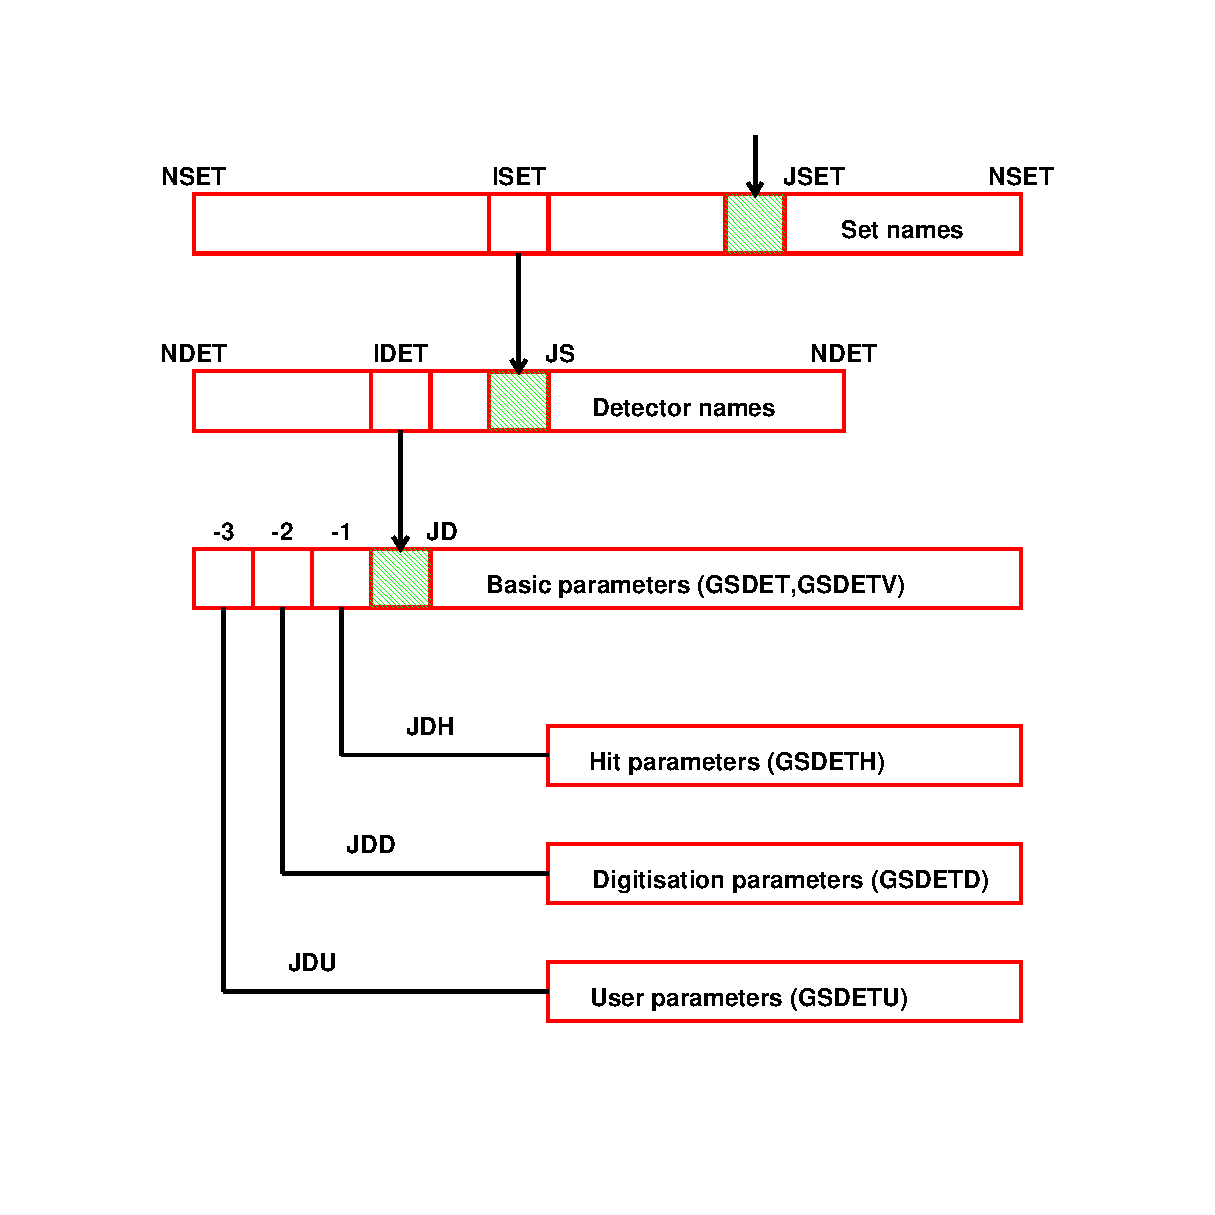
\epsfig{file=eps/hits199-1.eps,width=14cm}
     \caption{Example of geometrical tree structure}
     \label{fg:hits199-1}
\end{figure}
 
{\tt JS} = {\tt LQ(JSET-ISET)} pointer to detector set number {\tt ISET}
The {\tt JSET} data structure is filled by \Rind{GSDET}, 
\Rind{GSDETV}, \Rind{GSDETH}, \Rind{GSDETD}, \Rind{GSDETU} 
and possibly by \Rind{GSDETA}.
 

%%%%%%%%%%%%%%%%%%%%%%%%%%%%%%%%%%%%%%%%%%%%%%%%%%%%%%%%%%%%%%%%%%%
%                                                                 %
%  GEANT manual in LaTeX form                                     %
%                                                                 %
%  Michel Goossens (for translation into LaTeX)                   %
%  Version 1.00                                                   %
%  Last Mod. Jun  8 1993  1300   MG                               %
%                                                                 %
%%%%%%%%%%%%%%%%%%%%%%%%%%%%%%%%%%%%%%%%%%%%%%%%%%%%%%%%%%%%%%%%%%%
\Origin{R.Brun, F.Bruyant, W.Gebel, M.Maire}
\Submitted{01.11.83}                   \Revised{17.12.93}
\Version{Geant 3.16}                   \Routid{HITS200}

\Makehead{Routines to store and retrieve HITS}

\Shubr{GSAHIT}{(ISET,IDET,ITRA,NUMBV,HITS,IHIT*)}
\begin{DLtt}{MMMMMMMM}
\item[ISET]  ({\tt INTEGER}) set number (see below);
\item[IDET]  ({\tt INTEGER}) detector number;
\item[ITRA]  ({\tt INTEGER}) number of the track producing this hit
\item[NUMBV] ({\tt INTEGER}) array of volume numbers corresponding 
to list {\tt NAMESV} of {\tt GSDET};
\item[HITS] ({\tt REAL}) array of values for current hit elements;
\item[IHIT] ({\tt INTEGER}) current hit number, if 0 the
hit has not been stored.
\end{DLtt}

Stores element values for current hit into the data structure {\tt
JHITS}. The values {\tt ISET}, {\tt IDET} and {\tt NUMBV} can be found
in the corresponding variables of common \FCind{/GCSETS/}. These values
are set by the routine \Rind{GFINDS} every time that a particle is in
a defined detector.

\Shubr{GSCHIT}{(ISET,IDET,ITRA,NUMBV,HITS,NHSUM,IHIT*)}
Same action as \Rind{GSAHIT}, but in case the detector identified by
{\tt ISET}, {\tt IDET} and
{\tt NUMBV} contains already a hit for the same track, the routine will
make a cummulative sum for the latest {\tt NHSUM} elements of {\tt JHITS}.
The other previous elements of {\tt JHITS} are replaced.
That facility is particularly interesting in the case of
hits generated into a calorimeter. No packing (i.e. 32 bits per
hit element) should be requested for the
last {\tt NHSUM} hits in \Rind{GSDETH} and for these hits {\tt ORIG} should
be set to 0.

\Shubr{GPHITS}{(CHSET,CHDET)}
\begin{DLtt}{MMMMMMMM}
\item[CHSET] ({\tt CHARACTER*4}) set name,
if {\tt '*'} prints all {\tt JHITS} banks of all sets;
\item[CHDET] ({\tt CHARACTER*4}) detector name,
if {\tt '*'} prints hits in all detectors of set {\tt
CHSET}.
\end{DLtt}
Prints {\tt JHITS} banks for detector {\tt CHDET} of set {\tt CHSET}.
 
\Shubr{GFHITS}{(CHSET,CHDET,NVDIM,NHDIM,NHMAX,ITRS,NUMVS,
                ITRA*,NUMBV*,HITS*,NHITS*)}
 
\begin{DLtt}{MMMMMMMM}
\item[CHSET] ({\tt CHARACTER*4}) set name;
\item[CHDET] ({\tt CHARACTER*4}) detector name;
\item[NVDIM] ({\tt INTEGER}) 1$^{st}$ dimension of arrays {\tt NUMBV} and
{\tt NUMVS}: 1$\leq${\tt NVDIM}$\leq${\tt NV} argument of \Rind{GSDET};
\item[NHDIM] ({\tt INTEGER}) 1$^{st}$ dimension of array {\tt HITS}:
1$\leq${\tt NHDIM}$\leq${\tt NH} argument of \Rind{GSDETH};
\item[NHMAX] ({\tt INTEGER}) maximum number of hits to be returned, this 
should be not larger than the second dimension of array {\tt NUMBV} and
{\tt HITS};
\item[ITRS] ({\tt INTEGER}) number of the selected track,
if {\tt ITRS=0}, all tracks are taken;
\item[NUMVS] ({\tt INTEGER}) is a 1-dimension array of {\tt NVDIM}
elements that contains
the list of volume numbers which identify the selected detector,
0 is interpreted as 'all valid numbers';
\item[ITRA] ({\tt INTEGER}) is a 1-dim array of dimension {\tt NHMAX}
that contains on output
for each hit the number of the track which has produced it;
\item[NUMBV] ({\tt INTEGER}) 2-dim array ({\tt NVDIM,NHMAX})
that containis on output for each hit the
list of volume numbers which identify the detector, all values set to 
0 means that no more volumes are stored;
\item[HITS] ({\tt REAL}) 2-dim array ({\tt NHDIM,NHMAX}) that containis 
{\tt NHITS} hits;
\item[NHITS] ({\tt INTEGER}) number of hits returned, in case the total
number of hits is greater than {\tt NHMAX, NHITS} is set to
{\tt NHMAX+1} and {\tt NHMAX} hits are returned.
\end{DLtt}

This rotine returns the hits produced by track {\tt ITRS} (or by any track) in
the detector {\tt CHDET} identified by the list {\tt NUMVS}
belonging to set {\tt CHSET}.

\begin{DLtt}{MMMMMMMMMMMM}
\item[HITS(1,I)] is element 1 of hit number {\tt I};
\item[NUMBV(1,I)] is volume number 1 of hit number {\tt I};
\item[ITRA(I)] is the track number corresponding to hit number {\tt I};
\end{DLtt}

The arrays {\tt NUMVS, NUMBV, HITS}
and {\tt ITRA} must be dimensioned to:
\begin{verbatim}
    NUMVS(NVDIM)
    NUMBV(NVDIM,NHMAX)
    HITS(NHDIM,NHMAX)
    ITRA(NHMAX)
\end{verbatim}

\Shubr{GFPATH}{(ISET,IDET,NUMBV,NLEV*,LNAM*,LNUM*)}
\begin{DLtt}{MMMMMMMM}
\item[ISET] ({\tt INTEGER}) set number;
\item[IDET] ({\tt INTEGER}) detector number;
\item[NUMBV] ({\tt INTEGER}) array of numbers which identify uniquely
detector number {\tt IDET};
\item[NLEV] ({\tt INTEGER}) number of elements filled of arrays
{\tt LNAM} and {\tt LNUM};
\item[LNAM] ({\tt INTEGER}) array of {\tt NLEV} volume names stored in 
ASCII code in integers;
\item[LNUM] ({\tt INTEGER}) array of {\tt NLEV} copy numbers.
\end{DLtt}

This routine returns the list of volume names and numbers
which identify the complete ancestry in the {\tt JVOLUM} data structure of the
volume corresponding to the detector number {\tt IDET} in set
number {\tt ISET} and which is identified by the volume numbers {\tt NUMBV}
(see \Rind{GFHITS}).
 
\Rind{GFPATH} assumes that the detectors have been declared via 
\Rind{GSDETV} and not \Rind{GSDET}. The main use of \Rind{GFPATH} is to
prepare the lists {\tt LNAM} and {\tt LNUM} required  by the routine
\Rind{GLVOLU} to fill the common \FCind{/GCVOLU/}. Once \FCind{/GCVOLU/}
is properly filled, it is possible to use the {\tt GEANT} routines to
transform from the local to the master reference system and so on.
 

%%%%%%%%%%%%%%%%%%%%%%%%%%%%%%%%%%%%%%%%%%%%%%%%%%%%%%%%%%%%%%%%%%%
%                                                                 %
%  GEANT manual in LaTeX form                              %
%                                                                 %
%  Michel Goossens (for translation into LaTeX)                   %
%  Version 1.00                                                   %
%  Last Mod. Jan 24 1991  1300   MG + IB                          %
%                                                                 %
%%%%%%%%%%%%%%%%%%%%%%%%%%%%%%%%%%%%%%%%%%%%%%%%%%%%%%%%%%%%%%%%%%%
\Origin{R.Brun}
\Submitted{01.11.83}     \Revised{18.12.93}
\Version{Geant 3.16}     \Routid{HITS299}
\Makehead{The JHITS data structure}

\begin{figure}[hbt]
     \centering
     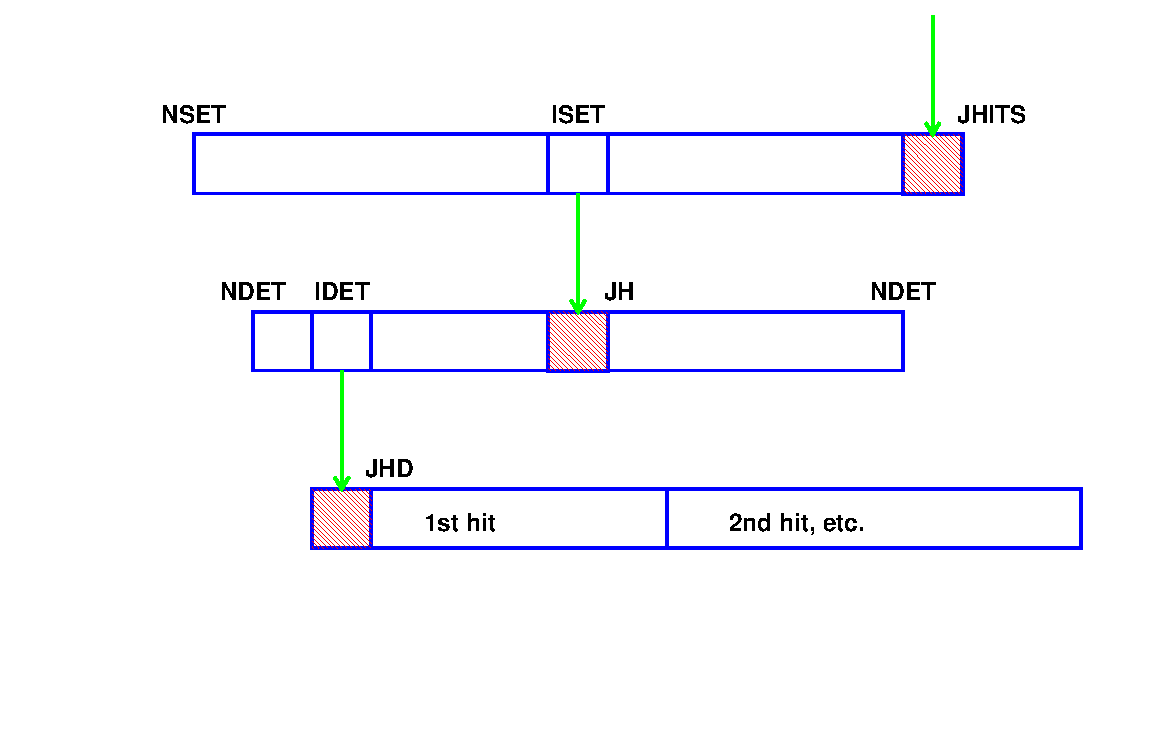
\epsfig{file=eps/hits299-1.eps,width=14cm}
     \caption{Layout of the {\tt JHITS} data structure}
     \label{fg:hits299-1}
\end{figure}

\begin{tabular}{lp{12cm}}
\tt JH=LQ(JHITS-ISET) & pointer to hits structure for set number {\tt ISET} \\
\tt IQ(JH+IDET) & number of words used for storing the hits
of detector number {\tt IDET} \\
\tt JHD=LQ(JH-IDET) & pointer to hits bank for detector number {\tt IDET} of
set number {\tt ISET} \\
\tt IQ(JHD+1) & 1$^{st}$ word of 1$^{st}$ hit \\
\tt IQ(JHD+NWH+1) & 1$^{st}$ word of 2$^{nd}$ hit \\
\tt JS=LQ(JSET-ISET) & pointer to the structure containing the description
of set number {\tt ISET} \\
\tt JD=LQ(JS-IDET) & pointer to the bank containing the description of detector
number {\tt IDET} of set number {\tt ISET} \\
\tt NWH=IQ(JD+3) & number of words in which a hit of detector
number {\tt IDET} of set number {\tt ISET} is stored
\end{tabular}

The {\tt JHITS} structure is filled with the routines \Rind{GSAHIT} and
\Rind{GSCHIT}.
The routine \Rind{GFHITS} can be used to get the hits for a detector
{\tt IDET} in set {\tt ISET}.

%%%%%%%%%%%%%%%%%%%%%%%%%%%%%%%%%%%%%%%%%%%%%%%%%%%%%%%%%%%%%%%%%%%
%                                                                 %
%  GEANT manual in LaTeX form                                     %
%                                                                 %
%  Version 1.00                                                   %
%                                                                 %
%  Last Mod.  9 Jun 1993  1300   MG                               %
%                                                                 %
%%%%%%%%%%%%%%%%%%%%%%%%%%%%%%%%%%%%%%%%%%%%%%%%%%%%%%%%%%%%%%%%%%%
\Origin{R.Brun, W.Gebel}
\Submitted{10.08.84}       \Revised{18.12.93}
\Version{Geant 3.16}       \Routid{HITS300}

\Makehead{Routines to store and retrieve DIGItisations}

\Shubr{GSDIGI}{(ISET,IDET,LTRA,NTRA,NUMBV,KDIGI,IDIG*)}
\begin{DLtt}{MMMMMMMM}
\item[ISET] ({\tt INTEGER}) set number;
\item[IDET] ({\tt INTEGER}) detector number;
\item[LTRA] ({\tt INTEGER}) array of {\tt NTRA} track numbers producing 
this digitisation;
\item[NUMBV] ({\tt INTEGER}) volume numbers corresponding to list {\tt NAMESV} 
of \Rind{GSDET};
\item[KDIGI] ({\tt INTEGER}) array of current digisation elements;
\item[IDIG] ({\tt INTEGER}) stored digitisation number, if 0, digitisation 
has not been stored.
\end{DLtt}
Stores element values for current digitisation
into the data structure {\tt JDIGI}.

\Shubr{GPDIGI}{(CHSET,CHDET)}
\begin{DLtt}{MMMMMMMM}
\item[CHSET] ({\tt CHARACTER*4}) set name,
if {\tt '*'} prints all {\tt JDIGI} banks of all sets;
\item[CHDET] ({\tt CHARACTER*4}) detector name, if {\tt '*'} prints 
digitisations in all detectors of set;
{\tt CHSET}
\end{DLtt}
Prints {\tt JDIGI} banks for detector {\tt CHDET} of set {\tt CHSET}.
 
\Shubr{GFDIGI}{(CHSET,CHDET,NTDIM,NVDIM,NDDIM,NDMAX,NUMVS,
                LTRA*,NTRA*,NUMBV*,KDIGI*,NDIGI*)}
\begin{DLtt}{MMMMMMMM}
\item[CHSET] ({\tt INTEGER}) set name;
\item[CHDET] ({\tt INTEGER}) detector name;
\item[NTDIM] ({\tt INTEGER}) 1$^st$ dimension of {\tt LTRA}, maxmum number of 
tracks contributing to each hit to be returned;
\item[NVDIM] ({\tt INTEGER}) 1$^{st}$ dimension of arrays {\tt NUMVS}, 
{\tt NUMBV}, same as argument {\tt NV} of \Rind{GSDET};
\item[NDDIM] ({\tt INTEGER}) 1$^{st}$ dimension of {\tt KDIGI}, same
as argument {\tt ND} of \Rind{GSDETD};
\item[NDMAX] ({\tt INTEGER}) maximum number of digitisations to be returned,
second dimension of arrays {\tt NTDIM}, {\tt NUMBV} and {\tt KDIGI};
\item[NUMVS] ({\tt INTEGER}) is a 1-dim array of length {\tt NVDIM}
that contains the copy numbers identifying the detector to be selected, all 
0 is interpreted as all copies of detector {\tt CHDET};
\item[LTRA] ({\tt INTEGER}) is a 2-dim array {\tt NTDIM,NDMAX} that contains
for each digitisation the numbers of the tracks which have produced it;
\item[NTRA] ({\tt INTEGER}) is a 1-dim array of length {\tt NDMAX} that contains,
for each digitisation, the number of tracks contributing,
in case this number is greater than {\tt NTDIM}, only the first
{\tt NTDIM} corresponding tracks are returned on {\tt LTRA};
\item[NUMBV] ({\tt INTEGER}) is a 2-dim array {\tt NVDIM,NDMAX} that contains,
for each digitisation, the
list of volume numbers which identify each detector;
\item[KDIGI] ({\tt INTEGER}) is a 2-Dim array {\tt NDDIM,NDMAX} that contains 
the {\tt NDIGI} digitisations returned;
\item[NDIGI] ({\tt INTEGER}) is the total number of digitisations in this 
detector,
in case the total number of digitisations is greater than {\tt NDMAX},
{\tt NDIGI} is set to {\tt NDMAX+1} and only {\tt NDMAX} digitisations are
returned.
\end{DLtt}
Returns the digitisations for the detector {\tt CHDET} identified by the list 
of copy numbers {\tt NUMVS} belonging to set {\tt CHSET}. The maning of
the variables is the following:

\begin{tabular}{lp{10cm}}
\tt KDIGI(1,I) & digitisation element 1 for digitisation number {\tt I} \\
\tt NUMBV(1,I) & first volume number for digitisation number {\tt I} \\
\tt LTRA (1,I) & number of the first track contributing to digitisation 
number {\tt I} \\
\end{tabular}

In the calling routine, the arrays {\tt LTRA, NTRA, NUMVS, NUMBV,
KDIGI} must be dimensioned to:
\begin{verbatim}
      LTRA (NTDIM,NDMAX)
      NTRA (NDMAX)
      NUMVS(NVDIM)
      NUMBV(NVDIM,NDMAX)
      KDIGI(NDDIM,NDMAX)
\end{verbatim}
 

%%%%%%%%%%%%%%%%%%%%%%%%%%%%%%%%%%%%%%%%%%%%%%%%%%%%%%%%%%%%%%%%%%%
%                                                                 %
%  GEANT manual in LaTeX form                              %
%                                                                 %
%  Michel Goossens (for translation into LaTeX)                   %
%  Version 1.00                                                   %
%  Last Mod. Jan 24 1991  1300   MG + IB                          %
%                                                                 %
%%%%%%%%%%%%%%%%%%%%%%%%%%%%%%%%%%%%%%%%%%%%%%%%%%%%%%%%%%%%%%%%%%%
\Origin{R.Brun}
\Submitted{01.11.83}     \Revised{18.12.93}
\Version{Geant 3.16}     \Routid{HITS399}
\Makehead{The JDIGI data structure}

\begin{figure}[hbt]
     \centering
     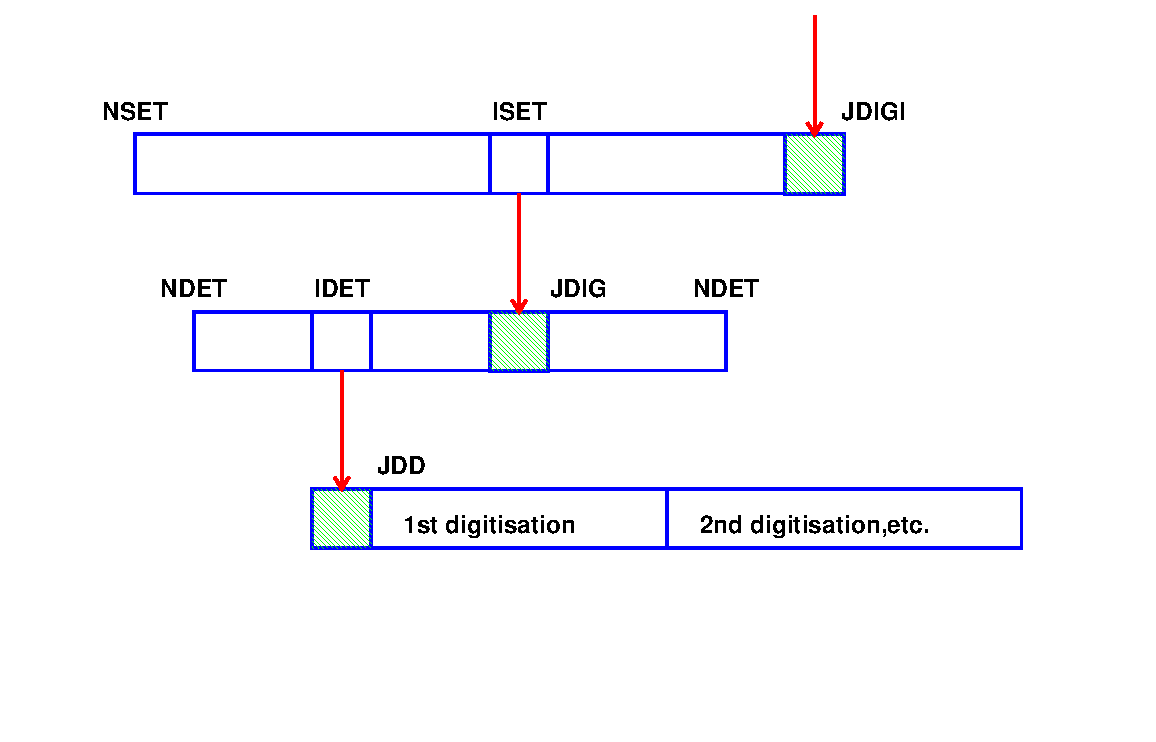
\epsfig{file=eps/hits399-1.eps,width=14cm}
     \caption{Layout of the {\tt JDIGI} data structure}
     \label{fg:hits399-1}
\end{figure}

\begin{tabular}{lp{10cm}}
\tt JDIG=LQ(JDIGI-ISET) & pointer to digitisations structure for set 
number {\tt ISET}\\
\tt JDD=LQ(JDIG-IDET) & pointer to digitisations of detector number
{\tt IDET} of set number {\tt ISET} \\
\tt IQ(JDIG+IDET) & pointer to last word of last digitisation for detector
number {\tt IDET} \\
\tt IQ(JDD+1) & 1$^{st}$ word of 1$^{st}$ digitisation \\
\tt IQ(JDD+N+1) & 1$^{st}$ word of 2$^{nd}$ digitisation\\
\tt JS=LQ(JSET-ISET) & pointer to the structure containing the description
of digitisations of set number {\tt ISET} \\
\tt JD=LQ(JS-IDET) & pointer to the structure containing the description
of digitisations of detector number {\tt IDET} \\
\tt NWD=IQ(JD+5) & number of elements of digitisation of set/detector
{\tt ISET}/{\tt IDET}  \\
\tt NTRA & number of tracks contributing to digitisation\\
\tt N=NWD+NTRA/2+1 & N varies from digitisation to digitisation 
\end{tabular}

The {\tt JDIGI} structure is filled with the routine \Rind{GSDIGI}.
The routine \Rind{GFDIGI} can be used to get the digitisations for
a detector {\tt IDET} in set {\tt ISET}.
 

%%%%%%%%%%%%%%%%%%%%%%%%%%%%%%%%%%%%%%%%%%%%%%%%%%%%%%%%%%%%%%%%%%%
%                                                                 %
%  GEANT manual in LaTeX form                                     %
%                                                                 %
%  Michel Goossens (for translation into LaTeX)                   %
%  Version 1.00                                                   %
%  Last Mod. Jan 24 1991  1300   MG + IB                          %
%                                                                 %
%%%%%%%%%%%%%%%%%%%%%%%%%%%%%%%%%%%%%%%%%%%%%%%%%%%%%%%%%%%%%%%%%%%
\Origin{R.Brun,H. Boerner}
\Submitted{01.10.81}   \Revised{18.12.93}
\Version{Geant 3.10}   \Routid{HITS400}

\Makehead{Intersection of a track with a cylinder or a plane}

\Shubr{GICYL}{(R,X1,X2,S1,S2,IC,XINT*,SINT*,PZINT*,IFLAG*)}
\begin{DLtt}{MMMMMMMM}
\item[R] ({\tt REAL}) radius of cylinder in cm;
\item[X1] ({\tt REAL}) array of 6, ($x$, $y$, $z$, $dx/ds$, 
$dy/ds$, $dz/ds$) of 1$^{st}$ point;
\item[X2] ({\tt REAL}) array of 6, ($x$, $y$, $z$, $dx/ds$, 
$dy/ds$, $dz/ds$) of 2$^{nd}$ point;
\item[S1] ({\tt REAL}) track length $s$ at 1$^{st}$ point;
\item[S2] ({\tt REAL}) track length $s$ at 2$^{nd}$ point;
\item[IC] ({\tt INTEGER}) type of interpolation:
\begin{DLtt}{MMMM}
\item[1] straight line defined as ({\tt Xi(1),Xi(2),Xi(3)}) + $s$
({\tt Xi(4),Xi(5),Xi(6)}), where {\tt i} is {\tt 1} or {\tt 2} according
to which of the two points is {\it inside} the cylinder;
\item[2] straight line going from ({\tt X1(1),X1(2),X1(3)}) to
({\tt X2(1),X2(2),X2(3)});
\item[3] third degree curve with:
\[
\vec{P}(s)  =  \vec{a} \; s^3 + \vec{b} \; s^2 +\vec{c} \; s +\vec{d} 
\hspace{1.2cm}
\mbox{\tt X}i   =  \left ( \vec{P}(\mbox{\tt S}i), \; 
\left . \frac{d\vec{P}}{ds} \right |_{s=\mbox{\tt S}i} \right ) \hspace{5mm}
i=1,2
\]
\end{DLtt}
\item[XINT] ({\tt REAL}) array of 6 $x$, $y$, $z$, $dx/ds$, $dy/ds$, $dz/ds$ 
at intersection point;
\item[SINT] ({\tt REAL}) {\tt S} at intersection point;
\item[PZINT] ({\tt REAL}) $\phi$, $z$, $d\phi/dr$, $dz/dr$ in
cylindrical coordinates at intersection point;
\item[IFLAG] ({\tt INTEGER}) return flag:
\begin{DLtt}{MMMM}
\item[0] track does not intersect cylinder;
\item[1] track intersects cylinder.
\end{DLtt}
\end{DLtt}
Calculates intersection of track with a cylinder
of radius {\tt R}. The track is approximated by a cubic
in the track length. To improve stability, the coordinate system
is shifted.

\Shubr{GIPLAN}{(YC,X1,X2,S1,S2,IC,XINT*,SINT*,PZINT*,IFLAG*)}
The arguments have the same meaning than in the previous routine, apart from:
\begin{DLtt}{MMMMMMMM}
\item[YC] ({\tt REAL}) $y$ coordinate of plane;
\end{DLtt}
Calculates intersection of track with a plane parallel to $x-z$.
The track is approximated by a cubic
in the track length. To improve stability, the coordinate system
is shifted.

{\bf Note}: the default accuracy is 10 microns. The value
of {\tt EPSI} (internal variable) must be changed for a better precision.

%%%%%%%%%%%%%%%%%%%%%%%%%%%%%%%%%%%%%%%%%%%%%%%%%%%%%%%%%%%%%%%%%%%
%                                                                 %
%  GEANT manual in LaTeX form                                     %
%                                                                 %
%  Michel Goossens (for translation into LaTeX)                   %
%  Version 1.00                                                   %
%  Last Mod. Jan 24 1991  1300   MG + IB                          %
%                                                                 %
%%%%%%%%%%%%%%%%%%%%%%%%%%%%%%%%%%%%%%%%%%%%%%%%%%%%%%%%%%%%%%%%%%%
\Origin{GEANT2}
\Submitted{01.10.81}   \Revised{19.12.93}
\Version{Geant 3.16}\Routid{HITS500}
\Makehead{Digitisation for drift- or MWP- Chambers}

\Shubr{GPDRIF}{(DETREP,HITREP,IOUT*)}
\begin{DLtt}{MMMMMMMM}
\item[DETREP] ({\tt REAL}) array of 6 with detector description:
\begin{DLtt}{MMMM}
\item[1] number of wires;
\item[2] wire spacing in cm;
\item[3] $\sin(\alpha)$;
\item[4] $\cos(\alpha)$;
\item[5] distance of wire 1 from the origin in cm;
\item[6] drift velocity (cm/nsec)
\end{DLtt}
\item[HITREP] ({\tt REAL}) array of 2 with track description:
\begin{DLtt}{MMMM}
\item[1] $x$ coordinate of intersection;
\item[2] $y$ coordinate of intersection;
\end{DLtt}
\item[IOUT] ({\tt INTEGER}) result of digitisation:
\begin{DLtt}{MMMM}
\item[1] wire number;
\item[2] drift time (signed to avoid left/right ambiguity).
\end{DLtt}
\end{DLtt}
Digitisation routine for a plane drift chamber. The drift chamber is supposed
to be in the $x-y$ plane. The normal to the wires in the $x-y$ plane and the
$z$ axis form an angle $\alpha$.

\Shubr{GCMWPC}{(DETREP,HITREP,IOUT*)}
\begin{DLtt}{MMMMMMMM}
\item[DETREP] ({\tt REAL}) array of 6 with detector description:
\begin{DLtt}{MMMM}
\item[1] number of wires;
\item[2] wire spacing (radians);
\item[3] $d\theta/dz$ along the wires;
\item[4] $\theta$ of a point on wire 1;
\item[5] $z$ of a point on wire 1 corresponding to $\theta$={\tt DETREP(4)};
\item[6] gap width;
\end{DLtt}
\item[HITREP] ({\tt REAL}) array of 4 with track description:
\begin{DLtt}{MMMM}
\item[1] $\theta$ coordinate of intersection;
\item[2] $z$ coordinate;
\item[3] $d\theta/dr$;
\item[4] $dz/dr$;
\end{DLtt}
\item[IOUT] ({\tt INTEGER}) array of 4 with result of digitisation:
\begin{DLtt}{MMMM}
\item[1] wire number (-1 if missing);
\item[2] cluster size;
\item[3] wire number of second cluster if any;
\item[4] cluster size;
\end{DLtt}
\end{DLtt}
Routine to compute one or two digitisations produced
by a hit on a cylindrical {\tt MWPC}. The chamber is a cylinder of thickness
{\tt DETREP(6)} which should be small compared with the radius.

\Shubr{GPMWPC}{(DETREP,HITREP,IOUT*)}
\begin{DLtt}{MMMMMMMM}
\item[DETREP] ({\tt REAL}) array of 6 with detector description:
\begin{DLtt}{MMMM}
\item[1] number of wires;
\item[2] wire spacing (radians);
\item[3] $\sin(\alpha)$;
\item[4] $\cos(\alpha)$;
\item[5] distance of wire 1 from the origin in cm;
\item[6] gap width;
\end{DLtt}
\item[HITREP] ({\tt REAL}) array of 4 with track description:
\begin{DLtt}{MMMM}
\item[1] $x$ coordinate of intersection;
\item[2] $y$ coordinate of intersection;
\item[3] $dx/dz$;
\item[4] $dy/dz$;
\end{DLtt}
\item[IOUT] ({\tt INTEGER}) array of 2 with result of digitisation:
\begin{DLtt}{MMMM}
\item[1] wire number (-1 if missing);
\item[2] cluster size;
\end{DLtt}
\end{DLtt}
Digitisation routine for a plane {\tt MWPC}.
 

%%%%%%%%%%%%%%%%%%%%%%%%%%%%%%%%%%%%%%%%%%%%%%%%%%%%%%%%%%%%%%%%%%%
%                                                                 %
%  GEANT manual in LaTeX form                              %
%                                                                 %
%  Michel Goossens (for translation into LaTeX)                   %
%  Version 1.00                                                   %
%  Last Mod. Jan 24 1991  1300   MG + IB                          %
%                                                                 %
%%%%%%%%%%%%%%%%%%%%%%%%%%%%%%%%%%%%%%%%%%%%%%%%%%%%%%%%%%%%%%%%%%%
\Origin{W.Mitaroff}
\Submitted{21.02.85}               \Revised{19.12.93}
\Version{Geant 3.16}               \Routid{HITS510}

\Makehead{Digitisation for drift chambers}

\Shubr{GCDRIF}{(RADD,ZMIN,ZMAX,DETREP,HITREP,IOUT*)}
\begin{DLtt}{MMMMMMMM}
\item[RADD] ({\tt REAL}) radius of cylindrical chamber in cm;
\item[ZMIN] ({\tt REAL}) $z$ of lower end of cylindrical chamber;
\item[ZMAX] ({\tt REAL}) $z$ of upper end of cylindrical chamber;
\item[DETREP] ({\tt REAL}) array of 8 with detector description:
\begin{DLtt}{MMMM}
\item[1] number of wires;
\item[2] wire spacing in $\phi$ (radians);
\item[3] cosine of wire angle with respect to the $z$ axis;
\item[4] sine of wire angle  with respect to the $z$ axis 
(signed like $d\phi/dz$);
\item[5] $d\phi/dz$ along wire;
\item[6] $\phi$ of point with $z=0$ on wire 1;
\item[7] drift velocity (cm nsec$^{-1}$);
\item[8] if $>0$ user routine \Rind{GUDTIM}
will be called to calculate drift time;
\end{DLtt}
\item[HITREP] ({\tt REAL}) array of 4 describing the track:
\begin{DLtt}{MMMM}
\item[1] $\phi$ coordinate of intersection;
\item[2] $z$ coordinate of intersection;
\item[3] $d\phi/dr$;
\item[4] $dz/dr$;
\end{DLtt}
\item[IOUT] ({\tt INTEGER}) array of 4 with digitisation information:
\begin{DLtt}{MMMM}
\item[1] wire number (1...{\tt NWI} with increasing phi), -1 if {\tt DETREP}
parameters are inconsistent;
\item[2] drift time in nsec, $>0$ if $\phi(hit)>\phi(wire)$;
\item[3] digitised current division information
(relative position of charge along wire, per mille);
\item[4] amount of charge deposited onto wire.
\end{DLtt}
\end{DLtt}
Digitisation routine for a cylindrical drift chamber.
 
\begin{figure}[hbt]
     \centering
%    \epsfig{file=eps/hits510-1.eps,width=14cm}
\begin{verbatim}
                        Charge                     
         .              |                        .
         |              .                        |
         =========================================  SENSE WIRE
     ...................................................> Z (cm)
         Z              Z                        Z 
          l                                       u
     ...............................................> ICD (0<ICD<1000)
         0              ICD                      1000
               ICD                (1000-ICD)
\end{verbatim}
     \caption{Coordinate system along the wire}
     \label{fg:hits510-1}
\end{figure}

Knowing the position $Z$ of the deposit of charge we can calculate
\[
\mbox{\tt ICD} = L \frac{Z-Z_l}{Z_u -Z_l} 
\]
where $L=1000$ in the
program. This is the information stored into {\tt IOUT(3)}.

\Shubr{GCDERR}{(ICD*,ERP,ERS)}
\begin{DLtt}{MMMMMMMM}
\item[ICD] ({\tt INTEGER}) digitised current division information 
($\leq\mbox{\tt ICD}\leq1000$), overwritten on output with the
modified value taking into account the errors;
\item[ERP] ({\tt REAL}) variance of Gaussian pedestal errors 
on the measured
pulse heights relative to the sum of the pulse heights;
\item[ERS] ({\tt REAL}) variance of Gaussian slope 
errors on the measured
pulse heights relative to the each pulse heights.
\end{DLtt}
Routine to calculate the error on the current division
information as obtained by \Rind{GCDRIF}.
Here we assume that {\tt ICD} has been determined by measuring the pulse heights 
$I_1, I_2$ at the two ends of the wire with the formula:
\[
\mbox{\tt ICD} = L \; \frac{I_2}{I_+} 
\mbox{\hspace{1cm}with\hspace{1cm}}  I_+ = I_1+I_2 
\]
Its error is determined by:
\[
\delta \mbox{\tt ICD} = - \frac{\mbox{\tt ICD}}{I_+} \delta I_1 + 
\frac{L-\mbox{\tt ICD}}{I_+}  \delta I_2
\mbox{\hspace{5mm}and\hspace{5mm}}
\delta I_1 = \delta_1 + \epsilon_1 \; I_1  \mbox{\hspace{3mm};\hspace{3mm}}
\delta I_2 = \delta_2 + \epsilon_2 \; I_2 
\]
 
 
$\delta_1$ and $\delta_2 $ are of dimension {\tt [I]} and represent the 
{\it pedestal} errors. $\epsilon_1$ and $\epsilon_2$ are the {\it slope} errors.
Errors are independent (no correlations), with a Gaussian distribution with 
average 0 and {\tt ERP} as relative variance for pedestals $\delta_i/I_+$ 
and {\tt ERS} as variance for slopes $\epsilon_i$.  This gives the final result
 
\[
\delta \mbox{\tt ICD}   = \underbrace{-\frac{\delta_1}{I_+}\mbox{\tt ICD} +
                 \frac{\delta_2}{I_+}(L-\mbox{\tt ICD})}_{\mbox{\it pedestals}}
               +
 \underbrace{(\epsilon_2-\epsilon_1)
\frac{\mbox{\tt ICD}(L-\mbox{\tt ICD})}{L}}_{\mbox{\it slope}}
\]

\Rind{GCDERR} sets the {\tt ICD} obtained from \Rind{GCDRIF} to
$\mbox{\tt ICD}=\mbox{\tt ICD}+\delta \mbox{\tt ICD}$ with 
$ 0 \leq \mbox{\tt ICD}\leq L$.

\Sfunc{GUDTIM}{VALUE = GUDTIM(DETREP,HITREP,IW1,DIS)}
The arguments have the same meaning than for \Rind{GCDRIF} apart from:
\begin{DLtt}{MMMMMMMM}
\item[IW1] ({\tt INTEGER}) wire number which will generate a signal;
\item[DIS] ({\tt REAL}) distance from the track to the wire;
\end{DLtt}
This function has to be written by the user to return the drift time
in nanoseconds.

\putbib[cnasbibl,geabibl]
\end{bibunit}
 
%%     IOPA part     %%
 
\begin{bibunit}[unsrt]
\renewcommand{\bibname}{IOPA Bibliography}
%%%%%%%%%%%%%%%%%%%%%%%%%%%%%%%%%%%%%%%%%%%%%%%%%%%%%%%%%%%%%%%%%%%
%                                                                 %
%  GEANT manual in LaTeX form                              %
%                                                                 %
%  Michel Goossens (for translation into LaTeX)                   %
%  Version 1.00                                                   %
%  Last Mod. Jan 24 1991  1300   MG + IB                          %
%                                                                 %
%%%%%%%%%%%%%%%%%%%%%%%%%%%%%%%%%%%%%%%%%%%%%%%%%%%%%%%%%%%%%%%%%%%
\Documentation{R.Brun}
\Submitted{15.08.84}          \Revised{16.12.93}
\Version{Geant 3.16}          \Routid{IOPA001}

\Makehead{The I/O  routines}
The I/O routines allow one to read, write or print the
{\tt GEANT} data structures. All {\tt GEANT} I/O is handled though
the {\tt ZEBRA} system, which provides the following facilities:
\begin{itemize}
\item native and machine independent I/O to and from disk and tape
devices;
\item sequential and direct access I/O (from disk);
\end{itemize}

This allows, for example, to generate events on one machine, dump
the data structures to a mass storage device, and then read them
back for further processing on a different machine.

This section describes the various routines for I/O in {\tt GEANT}.
For a complete reference on the {\tt ZEBRA} I/O system the user
is referred to the {\tt ZEBRA} documentation~\cite{bib-ZEBRAFZ,bib-ZEBRA}.

%%%%%%%%%%%%%%%%%%%%%%%%%%%%%%%%%%%%%%%%%%%%%%%%%%%%%%%%%%%%%%%%%%%
%                                                                 %
%  GEANT manual in LaTeX form                              %
%                                                                 %
%  Michel Goossens (for translation into LaTeX)                   %
%  Version 1.00                                                   %
%  Last Mod. Jan 24 1991  1300   MG + IB                          %
%                                                                 %
%%%%%%%%%%%%%%%%%%%%%%%%%%%%%%%%%%%%%%%%%%%%%%%%%%%%%%%%%%%%%%%%%%%
\Origin{R.Brun}
\Submitted{01.06.83}         \Revised{16.12.93}
\Version{Geant 3.16}         \Routid{IOPA200}
\Makehead{ZEBRA sequential files handling}

\Shubr{GOPEN}{(LUN,CHOPT,LEN,IER*)}
\begin{DLtt}{MMMMMMMM}
\item[LUN] ({\tt INTEGER}) logical unit number, 1$\leq${\tt LUN}$<$100;
\item[CHOPT] ({\tt CHARACTER*(*)}) any valid combination of
\Rind{FZFILE} options (see~\cite{bib-ZEBRAFZ,bib-ZEBRA}), the most common
being:
\begin{DLtt}{MMMM}
\item[I] input file;
\item[O] output file;
\item[X] exchange mode file;
\end{DLtt}
\item[LEN] ({\tt INTEGER}) maximum record length,
for more details see routine {\tt FZFILE} in the {\tt ZEBRA} manual;
\item[IER] ({\tt INTEGER}) error flag:
\begin{DLtt}{MMMM}
\item[0] legal open request;
\item[1] attempt to open more than 5 {\tt ZEBRA} sequential files;
\end{DLtt}
\end{DLtt}
Opens a {\tt ZEBRA} {\tt FZ} file for sequential I/O of {\tt GEANT}
data structures. No more than 5 files can be open at any one time.

\Shubr{GCLOSE}{(LUN,IER*)}
\begin{DLtt}{MMMMMMMM}
\item[LUN] ({\tt INTEGER}) logical unit to be closed, if 0 all {\tt ZEBRA}
{\tt FZ} streams will be closed;
\item[IER] ({\tt INTEGER}) error flag:
\begin{DLtt}{MMMM}
\item[0] legal close request;
\item[1] no unit was found open;
\end{DLtt}
\end{DLtt}
This routine closes one or all {\tt ZEBRA} {\tt FZ} file(s). This is a 
mandatory routines for all open {\tt ZEBRA} files before the end of the
program. Failure to call this routine may cause files to be incompletely
written to the storage media.
 
 

%%%%%%%%%%%%%%%%%%%%%%%%%%%%%%%%%%%%%%%%%%%%%%%%%%%%%%%%%%%%%%%%%%%
%                                                                 %
%  GEANT manual in LaTeX form                              %
%                                                                 %
%  Michel Goossens (for translation into LaTeX)                   %
%  Version 1.00                                                   %
%  Last Mod. Jan 24 1991  1300   MG + IB                          %
%                                                                 %
%%%%%%%%%%%%%%%%%%%%%%%%%%%%%%%%%%%%%%%%%%%%%%%%%%%%%%%%%%%%%%%%%%%
\Origin{R. Brun}
\Submitted{01.06.83}       \Revised{17.12.93}
\Version{Geant 3.16}       \Routid{IOPA300}
\Makehead{Data structure I/O with sequential files}
\Shubr{GFIN}{(LUN,CHOBJ,NKEYS,IDVERS*,CHOPT,IER*)}
\begin{DLtt}{MMMMMMMM}
\item[LUN] ({\tt INTEGER}) logical unit;
\item[CHOBJ] ({\tt CHARACTER*4}) array with the data structures to be read:
\begin{DLtt}{MMMMMM}
\item[MATE] material;
\item[TMED] tracking medium;
\item[VOLU] volumes;
\item[ROTM] rotation matrix;
\item[SETS] detector set;
\item[PART] particle;
\item[SCAN] scan geometry;
\item[DRAW] drawing;
\item[INIT] all of the above;
\item[KINE] this keyword will trigger the read of {\tt KINE} and {\tt VERT}
unless the flag {\tt S} is set;
\item[DIGI] digitisation;
\item[HEAD] event header;
\item[HITS] hits;
\item[RUNG] run;
\item[STAK] particle temporary stack;
\item[STAT] volume statistic;
\item[VERT] vertex;
\item[JXYZ] track points;
\item[TRIG] this keyword will trigger the read of
{\tt DIGI}, {\tt HEAD}, {\tt HITS}, {\tt KINE}, {\tt VERT} and {\tt JXYZ}
unless the {\tt S} flag is set;
\end{DLtt}
\item[NKEYS] ({\tt INTEGER})  number of keys in array {\tt CHOBJ};
\item[IDVERS] ({\tt INTEGER}) version of the data structure to be read in,
if 0 it will read any version, on output it contains the version of the
data structure read in;
\item[CHOPT] ({\tt CHARACTER*(*)})  option:
\begin{DLtt}{MMMM}
\item[I] among the data structures specified
in {\tt CHOBJ} read only the initialisation ones;
\item[K] among the data structures specified
in {\tt CHOBJ} read only {\tt KINE} and {\tt TRIG}, if present;
\item[T] among the data structures specified
in {\tt CHOBJ} read only {\tt DIGI}, {\tt HEAD}, {\tt HITS}, {\tt KINE},
{\tt VERT} and {\tt JXYZ}, if present; 
\item[S] interpret {\tt KINE} to mean only the {\tt KINE} data structure
and ignore {\tt TRIG} and {\tt INIT};
\item[Q] quiet option, no message is printed;
\end{DLtt}
\item[IER] ({\tt INTEGER}) error flag:
\begin{DLtt}{MMMM}
\item[$<$0] {\tt ZEBRA} error flag as returned in {\tt IQUEST(1)};
\item[~0] read completed successfully;
\item[$>$0] if only {\tt IER}] structures read in out of the {\tt NKEYS}
requested;
\end{DLtt}
\end{DLtt}

Routine to read {\tt GEANT} object(s) from a {\tt ZEBRA/FZ} file.
The data structures from disk are read in memory.
The {\tt FZ} data base must have been been created via 
\Rind{GOPEN}/\Rind{GFOUT}.  Example:
\begin{verbatim}
      CALL GOPEN(1,'I',1024,IER)
      IDVOLU = 0
      IDMATE = 0
      IDTMED = 0
      IDROTM = 0
      IDPART = 0
      IDSCAN = 0
      IDSETS = 0
      CALL GFIN (1,'VOLU',1,IDVOLU,' ',IER)
      CALL GFIN (1,'MATE',1,IDMATE,' ',IER)
      CALL GFIN (1,'TMED',1,IDTMED,' ',IER)
      CALL GFIN (1,'ROTM',1,IDROTM,' ',IER)
      CALL GFIN (1,'PART',1,IDPART,' ',IER)
      CALL GFIN (1,'SCAN',1,IDSCAN,' ',IER)
      CALL GFIN (1,'SETS',1,IDSETS,' ',IER)
\end{verbatim}


\Shubr{GFOUT}{(LUN,CHOBJ,NKEYS,IDVERS,CHOPT,IER*)}
The arguments have the same meaning than for \Rind{GFIN} with the following
differences:
\begin{DLtt}{MMMMMMMM}
\item[IDVERS] ({\tt INTEGER}) version identifier of the data structures
to be written out;
\end{DLtt}

Routine to write {\tt GEANT} object(s) into a {\tt ZEBRA/FZ} file.
The data structures from memory are written on the file.
The {\tt FZ} data base must have been been created via
\Rind{GOPEN}/\Rind{GFOUT}.  Example:

\begin{verbatim}
      CALL GOPEN(1,'O',1024,IER)
      CALL GFOUT (1,'VOLU',1,IDVOLU,' ',IER)
      CALL GFOUT (1,'MATE',1,IDMATE,' ',IER)
      CALL GFOUT (1,'TMED',1,IDTMED,' ',IER)
      CALL GFOUT (1,'ROTM',1,IDROTM,' ',IER)
      CALL GFOUT (1,'PART',1,IDPART,' ',IER)
      CALL GFOUT (1,'SCAN',1,IDSCAN,' ',IER)
      CALL GFOUT (1,'SETS',1,IDSETS,' ',IER)
\end{verbatim}

{\bf Note:} the routines \Rind{GGET} and \Rind{GSAVE} are obsolete and
should not be used.

%%%%%%%%%%%%%%%%%%%%%%%%%%%%%%%%%%%%%%%%%%%%%%%%%%%%%%%%%%%%%%%%%%%
%                                                                 %
%  GEANT manual in LaTeX form                              %
%                                                                 %
%  Michel Goossens (for translation into LaTeX)                   %
%  Version 1.00                                                   %
%  Last Mod. Jan 24 1991  1300   MG + IB                          %
%                                                                 %
%%%%%%%%%%%%%%%%%%%%%%%%%%%%%%%%%%%%%%%%%%%%%%%%%%%%%%%%%%%%%%%%%%%
\Origin{R.Brun}
\Submitted{20.08.87}        \Revised{17.12.93}
\Version{Geant 3.16}        \Routid{IOPA400}
\Makehead{ZEBRA direct access files handling}

I/O with direct access files is the most efficient way to use direct
access devices. All the routines described in this section and in
({\tt [IOPA500]}) are based on the {\tt ZEBRA-RZ} package and the
user is referred to the related documentation~\cite{bib-ZEBRA}
for an understanding of the basic principles.

\Shubr{GRFILE}{(LUN,CHFILE,CHOPT)}
\begin{DLtt}{MMMMMMMM}
\item[LUN] ({\tt INTEGER}) logical unit number;
\item[CHFILE] ({\tt CHARACTER*(*)}) file name;
\item[CHOPT] ({\tt CHARACTER*(*)}) any valid option for \Rind{RZOPEN},
\Rind{RZMAKE} and \Rind{RZFILE} and in particular:
\begin{DLtt}{MMMM}
\item[N] create a new file;
\item[U] open an existing file for update;
\item[Q] the initial allocation (default 1000 records)
is in {\tt IQUEST(10)};
\item[I] read all initialisation data structures (see description of 
\Rind{GRIN}/\Rind{GROUT}) from file to memory;
\item[O] write all initialisation data structures from memory to file;
\end{DLtt}
\end{DLtt}

This routine opens a file for direct access I/O of {\tt ZEBRA} data
structures. By default the file is opened in exchange mode and the option
{\tt W} is added, which creates an {\tt RZ} top level directory with the
name {\tt //LUNnn} where {\tt nn} is the logical unit number.

The default allocation of an {\tt RZ} directory is enough for 1000 records,
which allows for a 4Mb file with the standard record length of 1024 words. 
If a larger file is needed, the size of the directory should be changed 
when creating the file. This can be done by assigning to the variable
{\tt IQUEST(10)} in the common \FCind{/QUEST/} the requested number of records,
and calling \Rind{GRFILE} with the option {\tt Q} as shown in the following
example:
\begin{verbatim}
      COMMON / QUEST / IQUEST(100)
      .
      .
      .
      IQUEST(10) = 5000
      CALL GRFILE(1,'mygeom.geom','Q')
\end{verbatim}

\Shubr{GRMDIR}{(CHDIR,CHOPT)}

\begin{DLtt}{MMMMMMMM}
\item[CHDIR] ({\tt CHARACTER*(*)}) subdirectory name to create;
\item[CHOPT] option string:
\begin{DLtt}{MMMM}
\item[' '] create a subdirectory;
\item[S] create a subdirectory and set the current directory to it;
\end{DLtt}
\end{DLtt}
This routine creates an {\tt RZ} subdirectory.

\Shubr{GREND}{(LUN)}
\begin{DLtt}{MMMMMMMM}
\item[LUN] ({\tt INTEGER}) logical unit number (see \Rind{RZEND} in
the {\tt ZEBRA} manual~\cite{bib-ZEBRA});
\end{DLtt}
 
Routine to close an {\tt RZ} file. It is very important to call this
routine for all {\tt RZ} files open in write mode. Failure to do may
result in the files being incompletely written or corrupted.

%%%%%%%%%%%%%%%%%%%%%%%%%%%%%%%%%%%%%%%%%%%%%%%%%%%%%%%%%%%%%%%%%%%
%                                                                 %
%  GEANT manual in LaTeX form                              %
%                                                                 %
%  Michel Goossens (for translation into LaTeX)                   %
%  Version 1.00                                                   %
%  Last Mod. Jan 24 1991  1300   MG + IB                          %
%                                                                 %
%%%%%%%%%%%%%%%%%%%%%%%%%%%%%%%%%%%%%%%%%%%%%%%%%%%%%%%%%%%%%%%%%%%
\Origin{R.Brun}
\Submitted{20.08.87}      \Revised{17.12.93}
\Version{Geant 3.16}      \Routid{IOPA500}
\Makehead{Data structure I/O with direct access files}

\Shubr{GRIN}{(CHOBJ,IDVERS*,CHOPT)}
\begin{DLtt}{MMMMMMMM}
\item[CHOBJ] ({\tt CHARACTER*(4)}) name of the data structure to
read in, see {\tt [IOPA300]} for more information on this;
\item[IDVERS] ({\tt INTEGER}) version of the data structure to be read in,
if 0 it will read any version, on output it contains the version of the
data structure read in;
\item[CHOPT] ({\tt CHARACTER*(*)})  option:
\begin{DLtt}{MMMM}
\item[I] perform read only if
{\tt CHOBJ} is an initialisation data structure;
\item[K] perform read only if {\tt CHOBJ} is {\tt KINE} or {\tt TRIG};
\item[T] perform read only if {\tt CHOBJ} is 
{\tt DIGI}, {\tt HEAD}, {\tt HITS}, {\tt KINE},
{\tt VERT} or {\tt JXYZ};
\item[Q] quiet option, no message is printed;
\end{DLtt}
\end{DLtt}

This routine reads {\tt GEANT} data structures from the current working
directory of an {\tt RZ} file (see the {\tt ZEBRA} documentation for
a clarification of this concept). Example:
\begin{verbatim}

      CALL GRFILE(1,'Geometry.dat',' ')
      CALL GRIN ('VOLU',1,' ') 
      CALL GRIN ('MATE',1,' ')
      CALL GRIN ('TMED',1,' ')
      CALL GRIN ('ROTM',1,' ')
      CALL GRIN ('PART',1,' ')
      CALL GRIN ('SCAN',1,' ')
      CALL GRIN ('SETS',1,' ')
\end{verbatim}

The same result can be achieved by:
\begin{verbatim}

      CALL GRFILE(1,'Geometry.dat','I')
\end{verbatim}

\Shubr{GROUT}{(CHOBJ,IDVERS,CHOPT)}
The meaning of the arguments is the same than in the previous routine
\Rind{GRIN}, but for writing instead than for reading.

This routine writes {\tt GEANT} data structures into the current working
directory of an {\tt RZ} file (see the {\tt ZEBRA} documentation for
a clarification of this concept).
Note that if the cross-sections and energy loss tables
are available in the data structure {\tt JMATE}, then they are
saved on the data base.
The data structures saved by this routine can be retrieved
with the routine \Rind{GRIN}.
Before calling this routine a {\\tt RZ} data base must have been
created using \Rind{GRFILE}.
The data base must be closed with \Rind{RZEND}. Example:
\begin{verbatim}

      CALL GRFILE(1,'Geometry.dat','N')
      CALL GROUT ('VOLU',1,' ') 
      CALL GROUT ('MATE',1,' ')
      CALL GROUT ('TMED',1,' ')
      CALL GROUT ('ROTM',1,' ')
      CALL GROUT ('PART',1,' ')
      CALL GROUT ('SCAN',1,' ')
      CALL GROUT ('SETS',1,' ')
\end{verbatim}

The same result can be achieved by:
\begin{verbatim}

      CALL GRFILE(1,'Geometry.dat','NO')
\end{verbatim}

The interactive version of {tt GEANT} provides facilities
to interactively update, create and display objects.


The routines \Rind{GRGET} and \Rind{GRSAVE} are obsolete and should not 
be used.

\putbib[cnasbibl,geabibl]
\end{bibunit}
 
%%     KINE part     %%
 
\begin{bibunit}[unsrt]
\renewcommand{\bibname}{KINE Bibliography}
%%%%%%%%%%%%%%%%%%%%%%%%%%%%%%%%%%%%%%%%%%%%%%%%%%%%%%%%%%%%%%%%%%%
%                                                                 %
%  GEANT manual in LaTeX form                                     %
%                                                                 %
%  Version 1.00                                                   %
%                                                                 %
%  Last Mod.  8 June 1993 1300   MG                               %
%                                                                 %
%%%%%%%%%%%%%%%%%%%%%%%%%%%%%%%%%%%%%%%%%%%%%%%%%%%%%%%%%%%%%%%%%%%
\Submitted{28.04.86}        \Revised{15.12.93}
\Version{Geant 3.16}        \Routid{KINE001}

\Makehead{Section KINE}
This section describes the {\tt GEANT} kinematics structures {\tt JVERTX} and
{\tt JKINE} and the routines which permit one to store and retrieve the 
information. It also contains a short description of the {\tt GEANT} 
interface to the {\tt JETSET} generator and related routines.

%%%%%%%%%%%%%%%%%%%%%%%%%%%%%%%%%%%%%%%%%%%%%%%%%%%%%%%%%%%%%%%%%%%
%                                                                 %
%  GEANT manual in LaTeX form                              %
%                                                                 %
%  Michel Goossens (for translation into LaTeX)                   %
%  Version 1.00                                                   %
%  Last Mod. Jan 24 1991  1300   MG + IB                          %
%                                                                 %
%%%%%%%%%%%%%%%%%%%%%%%%%%%%%%%%%%%%%%%%%%%%%%%%%%%%%%%%%%%%%%%%%%%
\Origin{R.Brun}
\Revision{M.Maire}
\Documentation{R.Brun}
\Submitted{01.06.83}              \Revised{14.12.93}
\Version{Geant 3.16}              \Routid{KINE100}
\Makehead{Storing and retrieving vertex and track parameters}

\Shubr{GSVERT}{(VERT,NTBEAM,NTTARG,UBUF,NUBUF,NVTX*)}
 
\begin{DLtt}{MMMMMMMM}
\item[VERT] ({\tt REAL}) array of 3 containing the position of 
the vertex in the {\tt MRS};
\item[NTBEAM] ({\tt INTEGER}) beam track number origin of the vertex
(0 if none exists);
\item[NTTARG] ({\tt INTEGER}) target track number origin of the vertex
(0 if none exists);
\item[UBUF] ({\tt REAL}) user array of {\tt NUBUF} user words
to be stored in the data structure together with the vertex;
\item[NWBUF] ({\tt INTEGER}) number of user words;
\item[NVTX] ({\tt INTEGER}) number of the vertex stored (0 in case of error).
\end{DLtt}

This routine stores the parameters of a vertex to which tracks should be
attached via calls to \Rind{GSKINE}. Vertices are stored in the {\tt JVERTX}
data structure (see {\tt [KINE199]}) and they are preserved for the whole
duration of the event.

{\tt GEANT} tracks one vertex at a time: all the particles of one
vertex, and all the secondaries generated thereof must be transported
before the particles of the next vertex are considered.

This routine should be called only from \Rind{GUKINE} when the initial
kinematics of the event is defined. During tracking it is possible to add
vertices to the {\tt JVERTX} data structure, but this should be done via
the \Rind{GSKING} routine and the appropriate variables in the \FCind{/GCKING/}
common block. Please see {\tt [TRAK300]} for more information.

\Shubr{GSVERU}{(NVTX,NUBUF,UBUF,IADR*)}
\begin{DLtt}{MMMMMMMM}
\item[NVTX] ({\tt INTEGER}) vertex number;
\item[NUBUF] ({\tt INTEGER}) number of user words;
\item[UBUF] ({\tt REAL}) array of user words;
\item[IADR] ({\tt INTEGER}) position where information is stored in the
user bank of the vertex.
\end{DLtt}

This routine stores the first {\tt NUBUF} words of array {\tt BUF} in the
user bank attached to vertex {\tt NVTX}, starting at location {\tt IADR+1}.
On exit {\tt IADR} is set to {\tt IADR+NUBUF}, allowing subsequent filling. 
This allows effectively 
to {\it add} information to an existing vertex, whether or not it has already
an user buffer. This is the only way to add user information to a vertex
which has been created at tracking time by the routine \Rind{GSKING} via
an appropriate setting of parameters in the common \FCind{/GCKING/}.

\Shubr{GFVERT}{(NVTX,VERT*,NTBEAM*,NTTARG*,TOFG*,UBUF*,NUBUF*)}
Retrieves vertex parameters. The parameters have the same meaning
than the ones of \Rind{GSVERT}.
\begin{DLtt}{MMMMMMMM}
\item[TOFG] ({\tt REAL}) time of flight when the vertex was created;
\end{DLtt}

\Shubr{GPVERT}{(IVTX)}
 
Prints vertex parameters.
\begin{DLtt}{MMMMMMMM}
\item[IVTX] ({\tt INTEGER}) vertex number to be printed, all vertices if IVTX=0;
\end{DLtt}

\Shubr{GSKINE}{(PLAB,IPART,NV,UBUF,NUBUF,NT*)}
 
\begin{DLtt}{MMMMMMMM}
\item[PLAB] ({\tt REAL}) array of 3 containing the components of
the momentum of the particle in GeV c$^{-1}$;
\item[IPART] ({\tt INTEGER}) particle code (see {\tt [CONS300]});
\item[NV] ({\tt INTEGER}) number of the vertex origin of track;
\item[UBUF] ({\tt REAL}) array of {\tt NUBUF} user words
to be stored with the track;
\item[NUBUF] ({\tt INTEGER}) number of user words;
\item[NT] ({\tt INTEGER}) number of the stored track (0 in case of error).
\end{DLtt}

This routine stores the parameters of a track in the {\tt JKINE}
data structure (see {\tt [KINE199]}). This data structure survives for
the whole event, and it is wiped out by \Rind{GTRIGI} at the beginning 
of each new event.  There are two reasons to store tracks
in the {\tt JKINE} data structure:
\begin{itemize}
\item at the beginning of an event, from within \Rind{GUKINE}, to define
the initial kinematics of the event, i.e. the particles which {\tt GEANT}
will transport. This must be done through \Rind{GSKINE}
after that the vertices from which the particles originate have been defined
through \Rind{GSVERT};
\item during tracking, to preserve the kinematic information of a 
particular track till the end of the current event. In this case the user should
not call \Rind{GSKINE} directly, but rather set the appropriate flags in the
\FCind{/GCKING/} common block and call \Rind{GSKING}. This is explained in 
detail in {\tt [TRAK300]}.
\end{itemize}

\Shubr{GSKINU}{(NT,NUBUF,UBUF,IADR*)}
\begin{DLtt}{MMMMMMMM}
\item[NT] ({\tt INTEGER}) track number;
\item[NUBUF] ({\tt INTEGER}) number of user words;
\item[UBUF] ({\tt REAL}) array of user words;
\item[IADR] ({\tt INTEGER}) position where information is stored in the
user bank of the track.
\end{DLtt}

This routine stores the first {\tt NUBUF} words of array {\tt BUF} in the
user bank attached to track {\tt NT}, starting at location {\tt IADR+1}.
On exit {\tt IADR} is set to {\tt IADR+NUBUF}, allowing subsequent filling. 
This allows effectively 
to {\it add} information to an existing track, whether or not it has already
an user buffer. This is the only way to add user information to a track
which has been created at tracking time by the routine \Rind{GSKING} via
an appropriate setting of parameters in the common \FCind{/GCKING/}.

\Shubr{GFKINE}{(ITRA,VERT*,PVERT*,IPART*,NVERT*,UBUF*,NUBUF*)}
Retrieves long-life track parameters. The parameters have the same meaning
than the ones of \Rind{GSKINE}.

\Shubr{GPKINE}{(ITRA)}
Prints initial track parameters.
\begin{DLtt}{MMMMMMMM}
\item[ITRA] ({\tt INTEGER}) track to be printed, all tracks if {\tt IVTX}=0;
\end{DLtt}

%%%%%%%%%%%%%%%%%%%%%%%%%%%%%%%%%%%%%%%%%%%%%%%%%%%%%%%%%%%%%%%%%%%
%                                                                 %
%  GEANT manual in LaTeX form                              %
%                                                                 %
%  Michel Goossens (for translation into LaTeX)                   %
%  Version 1.00                                                   %
%  Last Mod. Jan 24 1991  1300   MG + IB                          %
%                                                                 %
%%%%%%%%%%%%%%%%%%%%%%%%%%%%%%%%%%%%%%%%%%%%%%%%%%%%%%%%%%%%%%%%%%%
\Origin{R.Brun}
\Submitted{01.11.83}      \Revised{14.12.93}
\Version{Geant 3.16}\Routid{KINE199}
\Makehead{The data structures JVERTX and JKINE}

\begin{figure}[hbt]
     \centering
     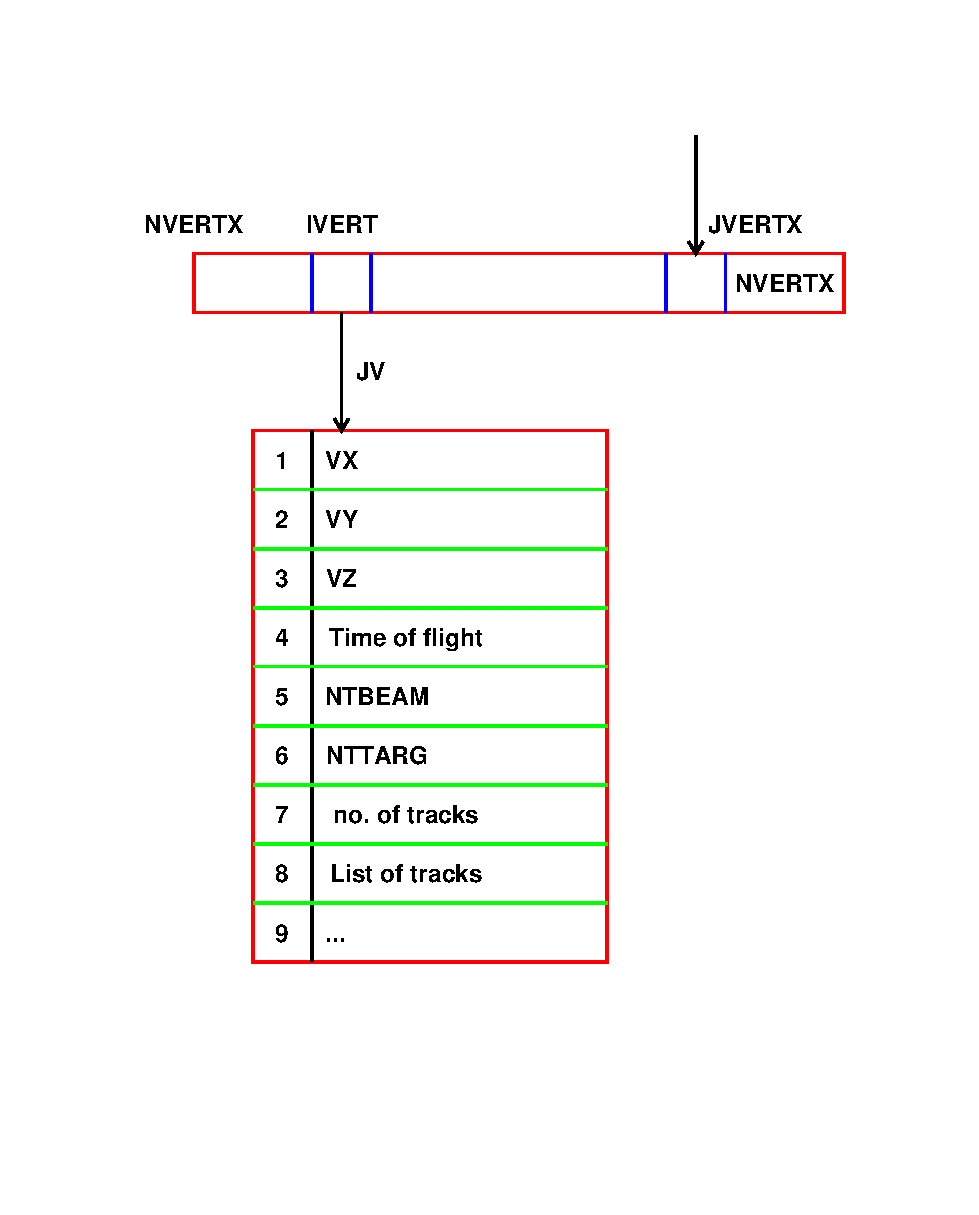
\epsfig{file=eps/kine199-1.eps,width=14cm}
     \caption{Layout of the {\tt JVERTX} data structure}
     \label{fg:kine199-1}
\end{figure}

\begin{DLtt}{MMMM}
\item[JV]= LQ(JVERTX-IVERT) pointer to the bank of vertex {\tt IVERT}.
\item[JVU]= {\tt LQ(JV-1)} pointer to the user part of the bank.
\end{DLtt}

The {\tt JVERTX} banks are filled by the routine \Rind{GSVERT} and \Rind{GSVERU}.
Vertex parameters can be retrieved by the routine \Rind{GFVERT} and printed
by the routine \Rind{GPVERT}.
 
\clearpage

\begin{figure}[hbt]
     \centering
     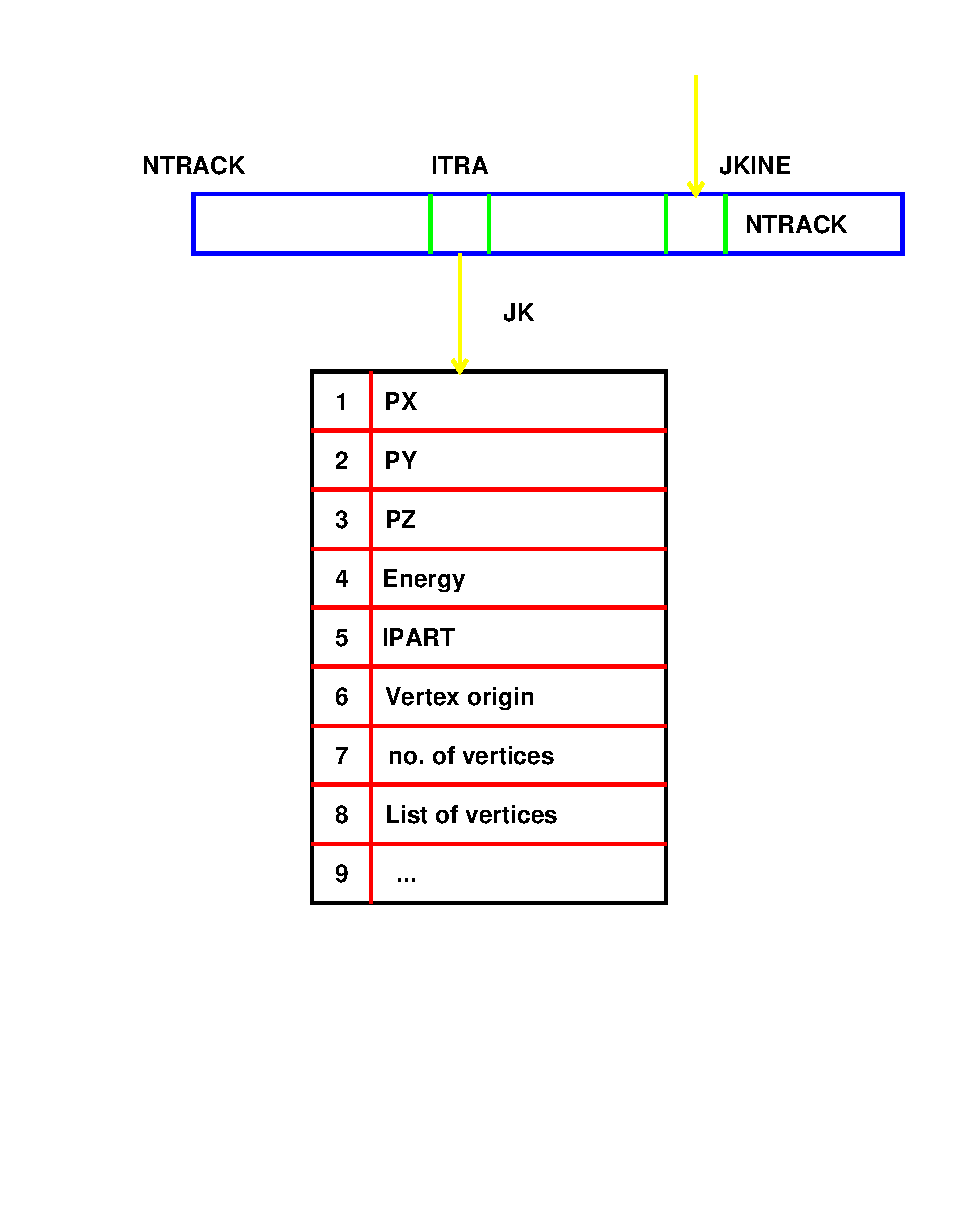
\epsfig{file=eps/kine199-2.eps,width=14cm}
     \caption{Layout of the {\tt JKINE} data structure}
     \label{fg:kine199-2}
\end{figure}

 
\begin{DLtt}{MMMM}
\item[JK]= {\tt LQ(JKINE-ITRA)} pointer to the bank of track {\tt ITRA}.
\item[JKU]= {\tt LQ(JK-1)} pointer to the user part of the bank.
\end{DLtt}
 
The {\tt JKINE} banks are filled by the routine \Rind{GSKINE} and \Rind{GSKINU}.
Track parameters can be retrieved by the routine \Rind{GFKINE} and printed
by the routine \Rind{GPKINE}.

%%%%%%%%%%%%%%%%%%%%%%%%%%%%%%%%%%%%%%%%%%%%%%%%%%%%%%%%%%%%%%%%%%%
%                                                                 %
%  GEANT manual in LaTeX form                                     %
%                                                                 %
%  Michel Goossens (for translation into LaTeX)                   %
%  Version 1.00                                                   %
%  Last Mod. Jan 24 1991  1300   MG + IB                          %
%                                                                 %
%%%%%%%%%%%%%%%%%%%%%%%%%%%%%%%%%%%%%%%%%%%%%%%%%%%%%%%%%%%%%%%%%%%
\Origin{R.Brun,R.Hemingway}
\Submitted{01.11.83}               \Revised{15.12.93}
\Version{Geant 3.16}               \Routid{KINE200}

\Makehead{Interface to the Lund Monte Carlo}

{\tt GEANT} contains a simple interface to the {\tt JETSET} Monte
Carlo generator~\cite{bib-JETS}. This interface is composed by an
initialisation routine and an event generation routine.

\Shubr{GLUNDI}{}
This is the initialisation routine which should be called before the
call to \Rind{GFFGO}, as it defines the data record {\tt LUND}. This routine
performs the following actions:
\begin{enumerate}
\item sets {\tt ECLUND}$=\sqrt{s}=92.25$ GeV;
\item sets {\tt IFLUND}$=0$;
\item activates initial state radiative effects {\tt MSTJ(107)= 1};
\item declares some particles ($K^0_s$, $\Sigma^{\pm}$, $\Xi^{\pm}$,
$\Lambda^0$, $\Omega^-$) to be stable in {\tt JETSET} so that {\tt GEANT}
can handle their tracking and decays:
\begin{verbatim}
         MDCY(LUCOMP(310) ,1)=0
         MDCY(LUCOMP(3222),1)=0
         MDCY(LUCOMP(3112),1)=0
         MDCY(LUCOMP(3322),1)=0
         MDCY(LUCOMP(3312),1)=0
         MDCY(LUCOMP(3122),1)=0
         MDCY(LUCOMP(3334),1)=0
\end{verbatim}
\end{enumerate}

Variables {\tt ECLUND}, total energy in the CMS, and {\tt IFLUND}, quark
flavours produced, are used as arguments for \Rind{LUEEVT} called by
\Rind{GLUND} and they can be changed via the {\tt LUND} data record
(see {\tt [BASE040]}).

\Shubr{GLUND}{}
Generate a \Pem\Pep collision via the {\tt JETSET} MonteCarlo and stores
the resulting final state particles for transport by {\tt GEANT}. All
particles are attached to a vertex in (0.,0.,0.). The {\tt K} and {\tt P}
arrays containing the full {\tt JETSET} event are copied in the user
buffer of the generated vertex, with the {\tt K} variables converted into
{\tt REAL} numbers. The content of the user buffer is the following:
\[
\begin{array}{ll}
\begin{array}{r@{}lc}
\mbox{\tt UBUF(} & \mbox{\tt 1)~} & 527.0 \\
\mbox{\tt UBUF(} & \mbox{\tt 2)~} & \mbox{{\tt N} number of particles}
\end{array} \\
\left .
\begin{array}{r@{}l@{\hspace{1cm}}l}
\mbox{\tt UBUF(} & \mbox{\tt 3)} & \mbox{\tt K(1,1)} \\
\mbox{\tt UBUF(} & \mbox{\tt 4)} & \mbox{\tt K(1,2)} \\
\mbox{\tt UBUF(} & \mbox{\tt 5)} & \mbox{\tt K(1,3)} \\
\mbox{\tt UBUF(} & \mbox{\tt 6)} & \mbox{\tt K(1,4)} \\
\mbox{\tt UBUF(} & \mbox{\tt 7)} & \mbox{\tt K(1,5)} \\
\mbox{\tt UBUF(} & \mbox{\tt 8)} & \mbox{\tt P(1,1)} \\
\mbox{\tt UBUF(} & \mbox{\tt 9)} & \mbox{\tt P(1,2)} \\
\mbox{\tt UBUF(} & \mbox{\tt 10)} & \mbox{\tt P(1,3)} \\
\mbox{\tt UBUF(} & \mbox{\tt 11)} & \mbox{\tt P(1,4)} \\
\mbox{\tt UBUF(} & \mbox{\tt 12)} & \mbox{\tt P(1,5)}
\end{array} \right \} & \mbox{{\tt N} times}
\end{array}
\]

%%%%%%%%%%%%%%%%%%%%%%%%%%%%%%%%%%%%%%%%%%%%%%%%%%%%%%%%%%%%%%%%%%%
%                                                                 %
%  GEANT manual in LaTeX form                              %
%                                                                 %
%  Michel Goossens (for translation into LaTeX)                   %
%  Version 1.00                                                   %
%  Last Mod. Jan 24 1991  1300   MG + IB                          %
%                                                                 %
%%%%%%%%%%%%%%%%%%%%%%%%%%%%%%%%%%%%%%%%%%%%%%%%%%%%%%%%%%%%%%%%%%%
\Origin{R.Hemingway}
\Submitted{01.11.83}         \Revised{15.12.93}
\Version{Geant 3.16}         \Routid{KINE210}
\Makehead{$\tau^{\pm}$ generation and decay}

\Shubr{GALL GTAU}{}
This routine is now dummy and it will only print an error message.
The appropriate routines from a generator Monte Carlo (for instance 
the {\tt JETSET}~\cite{bib-JETS} package)
should be used to handle $\tau^{\pm}$ production and decay.

\putbib[cnasbibl,geabibl]
\end{bibunit}
 
%%     PHYS part     %%
 
\begin{bibunit}[unsrt]
\renewcommand{\bibname}{PHYS Bibliography}
%%%%%%%%%%%%%%%%%%%%%%%%%%%%%%%%%%%%%%%%%%%%%%%%%%%%%%%%%%%%%%%%%%%
%                                                                 %
%  GEANT manual in LaTeX form                              %
%                                                                 %
%  Michel Goossens (for translation into LaTeX)                   %
%  Version 1.00                                                   %
%  Last Mod. Jan 24 1991  1300   MG + IB                          %
%                                                                 %
%%%%%%%%%%%%%%%%%%%%%%%%%%%%%%%%%%%%%%%%%%%%%%%%%%%%%%%%%%%%%%%%%%%
\Documentation{M. Maire, F.Carminati}
\Submitted{24.09.84}\Revised{26.07.93}
\Version{Geant 3.16}\Routid{PHYS001}
\Makehead{Introduction to the section PHYS}
\section{Summary of the physics processes}
 
The computer simulation of particles traversing an
experimental setup has to take into account the interactions of those
particles with the material of the detector.
{\tt GEANT} is able to simulate the dominant processes which can occur in the
energy range {\bf from 10 keV to 10 TeV} for electromagnetic interactions.
As far as hadronic interactions are concerned, the range of validity
is the one of the hadronic packages used, which usually does not extend
below a few tens of MeV. For more information the user is invited to 
consult the relevant 
documentation~\cite{bib-GHEI,bib-FLUK,bib-FLU1,bib-FLU2,bib-FLU3,bib-FLU4}.
 
Simulating a given process means:
\begin{UL}
\item
Evaluating the probability of occurrence of the process, by sampling the
{\bf total cross-section} of the process.
\item
Generating the final state after interaction, by sampling the
{\bf differential cross-section} of the process.
\item
In case of (quasi-)continuous processes, e.g. CSDA
(Continuous Slowing Down Approximation), energy losses or multiple 
scattering, computing the mean values of some characteristic quantities.
\end{UL}
In Table~\ref{phys001-1} below we summarise all the processes currently 
implemented in {\tt GEANT}, with a reference to the corresponding sections.
\begin{table}[hbt]
\begin{center}
\begin{tabular}{|l|l|l|}
\hline
& \parbox{5cm}{Computation of total cross-section or energy losses}
& \parbox{5cm}{Generation of the final state particles} \\
\hline
                                            &              &           \\
{\bf  Processes involving the photon }      &              &           \\
($e^+,e^-$ ) pair conversion                & PHYS 210     & PHYS  211 \\
Compton collision                           & PHYS 220     & PHYS  221 \\
Photoelectric effect                        & PHYS 230     & PHYS  231 \\
Photo fission of heavy elements             & PHYS 240     & PHYS  240 \\
Rayleigh effect                             & PHYS 250     & PHYS  251 \\
                                            &              &           \\
{\bf Processes involving $e^-/e^+ $ }       &              &           \\
Multiple scattering                         &              & PHYS 320
or 325 or 328\\
Ionisation and $\delta$-rays production     & PHYS 330     & PHYS 331
or 332 \\
Bremsstrahlung                              & PHYS 340      & PHYS 341 \\
Annihilation of positron                    & PHYS 350      & PHYS 351 \\
Generation of \v{C}erenkov light             & PHYS 260      & PHYS 260 \\
Synchrotron radiation                       & PHYS 360      &         \\
                                            &              &           \\
{\bf Processes involving}$\mu^-/ \mu^+$     &               &          \\
Decay in flight                             & CONS 310      & PHYS 400 \\
Multiple scattering                         &               & PHYS 320
or 325 \\
Ionisation and $\delta$-rays production     & PHYS 430      & PHYS 331
or 332 \\
Ionisation by heavy ions                    & PHYS 431      &         \\
Bremsstrahlung                              & PHYS 440      & PHYS 441 \\
Direct ($ e^+,e^-$) pair production         & PHYS 450      & PHYS 451 \\
Nuclear interaction                         & PHYS 460      & PHYS 460 \\
Generation of \v{C}erenkov light             & PHYS 260      & PHYS 260 \\
                                            &              &           \\
{\bf Processes involving hadrons}           &               &          \\
Decay in flight                             & CONS 310      & PHYS 400 \\
Multiple scattering                         &               & PHYS 320
or 325 \\
Ionisation and $\delta$-rays production     & PHYS 430      & PHYS 331
or 332 \\
Hadronic interactions                       & PHYS 500 or 510&
PHYS 500 or 510  \\
Generation of \v{C}erenkov light             & PHYS 260      & PHYS 260 \\
\hline
\end{tabular}
\end{center}
\label{phys001-1}
\caption{Processes currently implemented in {\tt GEANT}}
\end{table}
 
\subsection{ Simulated Processes }
 
\subsubsection{Hadronic Interactions}

To simulate the interactions of hadrons with the nuclei of the matter 
traversed, two alternatives are provided:
\begin{enumerate}
\item The generator of the \Rind{FLUKA}~\cite{bib-FLUK,bib-FLU1}
hadron shower MonteCarlo and the
interface routines to {\tt GEANT}. See {\tt [PHYS520]} for more information.
\item The generator of the \Rind{GHEISHA}~\cite{bib-GHEI}
hadron shower MonteCarlo and the
interface routines to {\tt GEANT}. See {\tt [PHYS510]} for more information.
\end{enumerate}
 
The code both of the \Rind{GHEISHA} and of the \Rind{FLUKA} generators is
contained in the {\tt GEANT} library. Users should be aware that the
routines of these packages do not follow the {\tt GEANT} naming conventions
and therefore they can clash with the names of user procedures.
 
\subsubsection{Electromagnetic Processes}
By means of systematic fits to the existing
data, the cross-sections of the electromagnetic processes are well reproduced
(within a few percent) from 10 keV up to 100 GeV, both for light (low Z) and
for heavy materials.
 
This feature, together with the use of the interface with one of the
hadronic shower generators available,
makes {\tt GEANT} useful also for shower simulation in gases.
 
\subsubsection{Muonic interactions}
Muonic interactions are simulated up to 10 TeV, making
{\tt GEANT} useful for cosmic rays studies.
 
\subsubsection{Ionisation by charged particles}
The following alternatives are provided to simulate this process:
\begin{itemize}
\item Sampling from the appropriate distribution around the mean value 
of the energy loss ({\tt [PHYS332]}).
\item
Explicit generation of $\delta$-rays (see {\tt [PHYS330/331/430]}) and 
restricted fluctuations below the energy threshold for the production
of $\delta$-rays.
\item
Sampling the contribution of single collisions from statistical 
distributions. This can be used as an alternative to the first one when
simulating energy losses 
in very thin layers (small value of g  cm$^{-2}$) (see {\tt [PHYS334]}).
\end{itemize}
Full Landau fluctuations and generation of $\delta$-rays cannot be used
together in order
to avoid double counting of the fluctuations. An automatic protection
has been introduced in {\tt GEANT} to this effect.
See {\tt [PHYS333/332]} and {\tt [BASE040]} for further information.
 
\subsubsection{Multiple Scattering}
Two methods are provided:
\begin{enumerate}
\item Moli\`ere distribution or plural scattering ({\tt [PHYS325], [PHYS328]}).
\item Gaussian approximation ({\tt [PHYS320]}).
\end{enumerate}
 
\subsubsection{The JMATE data structure}
In order to save time during the transport of the particles, relevant 
energy-dependent quantities are tabulated at the beginning of the run, for 
all materials, as functions of the kinetic energy of the particle.
In particular, the inverse of the total cross-sections 
of all processes involving photons, electrons and muons and the $dE/dx$ and 
range tables for electrons, muons and protons are calculated.
The actual value of, say, the interaction length for a given process (i.e. the
inverse of the macroscopic cross section) is then obtained via a linear
interpolation in the tables. The data structure which contains all this
information in memory is supported by the link {\tt JMATE} in the 
\FCind{/GCLINK/} common block.
See {\tt [PHYS100]} and {\tt [CONS199]} for a more information on these tables.
 
\subsubsection{Probability of Interaction}
The total cross-section of each process is used at tracking time to evaluate 
the probability of occurrence of the process. See {\tt [PHYS010]} for an 
explanation of the method used.
 
{\bf Note}: The section {\tt PHYS} is closely related to the section {\tt CONS}.
Users wishing to have a complete overview of the physics processes
included in {\tt GEANT} should read both sections.

\subsection{ Control of the physical processes}
 
For most of the individual processes the default option (indicated
below) can be changed via data records {\tt [BASE040]}.
The processes are controlled via a control variable which is in the
common \FCind{/GCKING/}. 
If not otherwise noted, 
the meaning of the control variable is the following:
\begin{DLtt}{MMM}
\item[= 0] The process is completely ignored. 
\item[= 1] The process is considered and possible secondary particles generating
from the interaction are put into the \FCind{/GCKING/} common. If the
interacting particle disappears in the interaction, then it is stopped
with {\tt ISTOP=1} (common \FCind{/GCTRAK/})
\item[= 2] The process is considered. If secondary particles result from the
interaction, they are not generated and their energy is simply added in the
variable {\tt DESTEP} (common \FCind{/GCTRAK/}. If the interacting particle
disappears in the interaction, the variable {\tt ISTOP} is set
to $2$.
\end{DLtt}
Below are listed the data record keywords, the flag names and values, and
the resulting action:

\begin{DLtt}{MMMMMMMM}
\item[Keyword] Related process 
\item[DCAY] Decay in flight. The decaying particles stops.
The variable {\tt IDCAY} controls this process.
\begin{DLtt}{MMMMMMMM}
\item[IDCAY =0] No decay in flight.
\item[~~~~~~=1] ({\bf D}) Decay in flight with generation of secondaries.
\item[~~~~~~=2] Decay in flight without generation of secondaries.
\end{DLtt}
\item[MULS] Multiple scattering. The variable {\tt IMULS} controls this process.
\begin{DLtt}{MMMMMMMM}
\item[IMULS =0] No multiple scattering.
\item[~~~~~~=1] ({\bf D}) Multiple scattering according to Moli\`ere theory.
\item[~~~~~~=2] Same as {\tt 1}. Kept for backward compatibility.
\item[~~~~~~=3] Pure Gaussian scattering according to the Rossi formula.
\end{DLtt}
\item[PFIS] Nuclear fission induced by a photon. The photon stops.
The variable {\tt IPFIS} controls this process.
\begin{DLtt}{MMMMMMMM}
\item[IPFIS =0] ({\bf D}) No photo-fission.
\item[~~~~~~=1] Photo-fission with generation of secondaries.
\item[~~~~~~=2] Photo-fission without generation of secondaries.
\end{DLtt}
\item[MUNU] Muon-nucleus interactions. The muon is not stopped.
The variable {\tt IMUNU} controls this process.
\begin{DLtt}{MMMMMMMM}
\item[IMUNU =0] No muon-nucleus interactions.
\item[~~~~~~=1] ({\bf D}) Muon-nucleus interactions with generation of 
secondaries.
\item[~~~~~~=2] Muon-nucleus interactions without generation of secondaries.
\end{DLtt}
\item[LOSS] Continuous energy loss. The variable {\tt ILOSS} controls this 
process.
\begin{DLtt}{MMMMMMMM}
\item[ILOSS =0] No continuous energy loss,IDRAY is forced to 0.
\item[~~~~~~=1] Continuous energy loss with generation of $\delta$-rays 
above {\tt DCUTE} (common \FCind{/GCUTS/}) and
restricted Landau fluctuations below {\tt DCUTE}.
\item[~~~~~~=2] ({\bf D}) Continuous energy loss without generation of 
$\delta$-rays
and full Landau-Vavilov-Gauss fluctuations. In this case the variable {\tt IDRAY}
is forced to $0$ to avoid double counting of fluctuations.
\item[~~~~~~=3] Same as $1$, kept for backward compatibility.
\item[~~~~~~=4] Energy loss without fluctuation. The value obtained from the
tables is used directly.
\end{DLtt}
\item[PHOT] Photoelectric effect. The interacting photon is stopped.
The variable {\tt IPHOT} controls this process.
\begin{DLtt}{MMMMMMMM}
\item[IPHOT =0] No photo-electric effect.
\item[~~~~~~=1] ({\bf D}) Photo-electric effect with generation of the electron.
\item[~~~~~~=2] Photo-electric effect without generation of the electron.
\end{DLtt}
\item[COMP] Compton scattering. The variable {\tt ICOMP} controls this process.
\begin{DLtt}{MMMMMMMM}
\item[ICOMP =0] No Compton scattering.
\item[~~~~~~=1] ({\bf D}) Compton scattering with generation of \Pem.
\item[~~~~~~=2] Compton scattering without generation of \Pem.
\end{DLtt}
\item[PAIR] Pair production. The interacting $\gamma$ is stopped.
The variable {\tt IPAIR} controls this process.
\begin{DLtt}{MMMMMMMM}
\item[IPAIR =0] No pair production.
\item[~~~~~~=1] ({\bf D}) Pair production with generation of \Pem/\Pep.
\item[~~~~~~=2] Pair production without generation of \Pem/\Pep.
\end{DLtt}
\item[BREM] bremsstrahlung. The interacting particle (\Pem, \Pep, $\mu^{+}$,
$\mu^{-}$) is not stopped.
The variable {\tt IBREM} controls this process.
\begin{DLtt}{MMMMMMMM}
\item[IBREM =0] No bremsstrahlung.
\item[~~~~~~=1] ({\bf D}) bremsstrahlung with generation of $\gamma$.
\item[~~~~~~=2] bremsstrahlung without generation of $\gamma$.
\end{DLtt}
\item[RAYL] Rayleigh effect. The interacting $\gamma$ is not stopped.
The variable {\tt IRAYL} controls this process.
\begin{DLtt}{MMMMMMMM}
\item[IRAYL =0] ({\bf D}) No Rayleigh effect.
\item[~~~~~~=1] Rayleigh effect.
\end{DLtt}
\item[DRAY] $\delta$-ray production. 
The variable {\tt IDRAY} controls this process.
\begin{DLtt}{MMMMMMMM}
\item[IDRAY =0] No $\delta$-rays production.
\item[~~~~~~=1] ({\bf D}) $\delta$-rays production with generation of \Pem.
\item[~~~~~~=2] $\delta$-rays production without generation of \Pem.
\end{DLtt}
\item[ANNI] Positron annihilation. The \Pep is stopped.
The variable {\tt IANNI} controls this process.
\begin{DLtt}{MMMMMMMM}
\item[IANNI =0] No positron annihilation.
\item[~~~~~~=1] ({\bf D}) Positron annihilation with generation of photons.
\item[~~~~~~=2] Positron annihilation without generation of photons.
\end{DLtt}
\item[HADR] Hadronic interactions. The particle is stopped in case of
inelastic interaction, while it is not stopped in case of elastic interaction.
The variable {\tt IHADR} controls this process.
\begin{DLtt}{MMMMMMMM}
\item[IHADR =0] No hadronic interactions.
\item[~~~~~~=1] ({\bf D}) Hadronic interactions with generation of secondaries.
\item[~~~~~~=2] Hadronic interactions without generation of secondaries.
\item[~~~~~~$>$2] Can be used in the user code \Rind{GUPHAD} and \Rind{GUHADR}
to chose a hadronic package. These values have no effect on the hadronic
packages themselves.
\end{DLtt}
\item[LABS] Light ABSorption. This process is the absorption of light photons
(particle type 7) in dielectric materials. It is turned on by default when
the generation of \v{C}erenkov light is requested (data record {\tt CKOV}).
For more information see {\tt [PHYS260]}.
\begin{DLtt}{MMMMMMMM}
\item[ILABS =0] No absorption of photons.
\item[~~~~~~=1] Absorption of photons with possible detection.
\end{DLtt}
\item[STRA]
This flag turns on the collision sampling method to simulate energy
loss in thin materials, particularly gases. For more information see
{\tt [PHYS334]}.
\begin{DLtt}{MMMMMMMM}
\item[ISTRA =0] ({\bf D}) Collision sampling switched off.
\item[~~~~~~=1] Collision sampling activated.
\end{DLtt}
\item[SYNC] Synchrotron radiation in magnetic field.
\begin{DLtt}{MMMMMMMM}
\item[ISYNC =0] ({\bf D}) The synchrotron radiation is not simulated.
\item[~~~~~~=1] Synchrotron photons are generated,
at the end of the tracking step.
\item[~~~~~~=2] Photons are not generated, the energy is deposit locally.
\item[~~~~~~=3] Synchrotron photons are generated,
distributed along the curved path of the particle.
\end{DLtt}
\end{DLtt}

%%%%%%%%%%%%%%%%%%%%%%%%%%%%%%%%%%%%%%%%%%%%%%%%%%%%%%%%%%%%%%%%%%%
%                                                                 %
% GEANT manual in LaTeX form                                      %
%                                                                 %
% Michel Goossens (for translation into LaTeX)                    %
% Version 1.00                                                    %
% Last Mod. Jan 24 1991 1300  MG + IB                             %
%                                                                 %
%%%%%%%%%%%%%%%%%%%%%%%%%%%%%%%%%%%%%%%%%%%%%%%%%%%%%%%%%%%%%%%%%%%
\hyphenation{bre-ms-strah-lung}
\Documentation{M. Maire, F.Carminati}
\Submitted{20.12.84}\Revised{26.07.93}
\Version{Geant 3.16}\Routid{PHYS010}
\Makehead{Compute the occurrence of a process}
\section {Principle}
The simulation of the processes which accompany the propagation of a
particle through the material of the detector
(e.g. bremsstrahlung,
$\delta$-rays production, Compton scattering and so on)
is performed by {\tt GEANT} in the following steps:
\begin{enumerate}
\item Fetch a new particle to be tracked (often called {\it track} or
{\it history}) from the stack supported by the link {\tt JSTAK} (see 
{\tt [TRAK399]}). This is done once at the beginning of each new track. 
The number of {\it interaction lengths} that the particle is going to 
travel, before undergoing each one of the possible discrete processes, 
is sampled at this point. These operations are done in the routine 
\Rind{GLTRAC}.
\item Evaluate the distance to the interaction point.
This is done by the individual tracking routines
(\Rind{GTGAMA}, \Rind{GTNEUT}, \Rind{GTHADR}, \Rind{GTNINO},
\Rind{GTMUON}, \Rind{GTHION} and \Rind{GTCKOV}) which control the 
tracking of particular particles.
The number of interaction lengths remaining to travel
before each of the
possible processes (often called {\it tracking mechanisms} or simply
{\it mechanisms}) is multiplied
by the inverse of the macroscopic cross-section
for that process in the current material (i.e. the interaction
length). This gives the distances that the particle has to travel before
each of the processes occurs in the current medium. 
The minimum among these numbers is the
{\it step} over which the particle will be transported. In addition to
the physics mechanisms, four
{\it pseudo-interactions} are taken into account in the calculation of
the step:
\begin{enumerate}
\item boundary crossing. The crossing of a volume boundary is treated
like a discrete process. A particle never crosses a boundary
during a step but rather stops there ({\tt NEXT} mechanism);
\item maximum step limit. For each tracking medium a value for the
maximum step can be specified by the user. Process {\tt SMAX};
\item maximum fraction of continuum energy loss, maximum angular
deviation in magnetic
field or maximum step for which the Moli\`ere formula, to simulate
multiple scattering is valid. These are continuous processes,
which introduce a limitation on the tracking step expressed by a
single variable (see section {\tt [PHYS325]} on \Rind{GMULOF}).
\item energy and time cut. Charged particles in matter are stopped when their
energy falls below their energy threshold or when their time of flight
exceeds the time cut;
\end{enumerate}
More information is given in the
individual sections explaining the implementation of the physical
processes.
\item Transport the particle either along a
straight line (if no magnetic field or for a
neutral particle) or along a helicoidal
path (for charged particles in magnetic field).
\item Update the energy of the particle if continuous energy loss was
in effect (charged particles in matter).
\item If a physical discrete process has been selected,
generate the final state of the interaction.
\item  If
the incident particle {\it survives} the interaction
(Compton, $\delta$-rays production, bremsstrahlung, direct pair
production by $\mu$ and $\mu$-nucleus interaction, hadronic elastic
scattering), sample
again the number of interaction lengths to travel before the next
event of the same kind. This is generally done by specialised routines:
\Rind{GMUNU}, \Rind{GCOMP}, \Rind{GBREM}, etc.
\item Update the number of interaction
lengths for all the processes and go back to $(2)$ till the particle
either leaves the detector or falls below its energy threshold or
beyond its time cut or disappears in an interaction.
\end{enumerate}
\section{Distance evaluation}
\subsection{The interaction length}
Let $\sigma(E,Z,A)$ be the total microscopic
cross section for a given interaction.
The mean free path, $\lambda$, for a particle to interact is given by:
\begin{equation}
\lambda  = \frac{1}{\Sigma}
\end{equation}
 
where $\Sigma$ is the macroscopic cross-section in $cm^{-1}$. This quantity
is given for an element by:
 
\begin{equation}
\Sigma  = \frac{N_{Av} \rho\sigma (E,Z,A)}{A}
\end{equation}
 
and for a compound or a mixture by:
 
\begin{equation}
\Sigma  = \frac{N_{Av}\rho \sum_i
          n_i\sigma(E,Z_i,A_i)}{\sum_i
          n_iA_i}
        = N_{Av} \rho \sum_i \frac{p_i}{A_i}\: \sigma(E,Z_i,A_i)
\end{equation}
 
\begin{tabular}[t]{ll}
$N_{Av}$         & Avogadro's number ($6.02486 \times 10^{23}$) \\
$Z$         & atomic number  \\
$A$         & atomic weight  \\
$\rho$    & density \\
$\sigma$  & total cross-section for the reaction \\
$n_i$   & \parbox[t]{14cm}{proportion by number of the $i^{th}$  
element in the material} \\
$p_i$ & \parbox[t]{14cm}{$=n_{i} A_{i}/ \sum_j n_jA_j$, proportion by 
weight of the $i^{th}$ element in the material}
\end{tabular}
 
For electromagnetic processes which depend linearly on the atomic number 
$Z$ we can write:

\begin{eqnarray*}
\Sigma(E)  & =  & N_{Av} \rho \sum_i \frac{p_i}{A_i}\: \sigma(E,Z_i) =
N_{Av} \rho \sum_i \frac{p_i}{A_i}\: Z_i f(E) \\
& = & N_{Av} \rho f(E) \sum_i \frac{p_i}{A_i}\: Z_i = N_{Av} \rho f(E) Z_{eff} \\
Z_{eff} & = & \sum_i \frac{p_i}{A_i}\: Z_i 
\end{eqnarray*}

the value above of $Z_{eff}$ is calculated by \Rind{GPROBI}.
This mean free path is tabulated at initialisation time as a function
of the kinetic energy of the particle, or, for hadronic interactions,
it is calculated at tracking time.

Cross sections are tabulated in the energy range defined as: 
$\mbox{\tt ELOW(1)} \leq E \leq \mbox{\tt ELOW(NEK1)}$
in {\tt NEK1} bins. These values can be redefined by the data record
{\tt RANGE}. Default values are $\mbox{\tt ELOW(1)} = 10 keV$,
$\mbox{\tt ELOW(NEK1)} = 10 TeV$ and $\mbox{\tt NEKBIN} = 
\mbox{\tt NEK1}-1 = 90$. {\tt NEKBIN} cannot be bigger than 199.
The array {\tt ELOW} is in the common \FCind{/GCMULO/}.

Numerically, if we measure the microscopic
cross section in $b$ where $1b=10^{-24}
cm^{-2}$, we can express the macroscopic cross section as:
\begin{eqnarray}
\Sigma [cm^{-1}]  & = & \frac{6.02486 \times 10^{23} \rho
[g \: cm^{-3}] \sigma (E,Z,A) [b] \times 10^{-24}}{A} \\
& = & 0.602486 \: \frac{\rho [g \: cm^{-3}]}{A} \: \sigma (E,Z,A) [b]
\end{eqnarray}

which is the formula mostly used in {\tt GEANT}.
\subsection{Determination of the interaction point}
The mean free path of a particle for a given process,
$\lambda$, depends on the medium and cannot be used
directly to sample the probability of an interaction in a heterogeneous
detector. The number of mean free paths which a particle travels is:
\[
N_\lambda =\int \frac{dx}{\lambda(x)}
\]
and it is independent of the material traversed. If $N_R$ is
a random variable denoting the number of mean free paths from a given
point until the point of interaction, it can be shown that $N_R$ has the
distribution function
\[
P( N_R < N_\lambda ) = 1-e^{-N_\lambda}
\]
The total number of mean free paths the particle travels before
the interaction point, $N_\lambda$, is sampled at the beginning
of the trajectory as:
\begin{displaymath}
N_\lambda = -\log \left ( \eta \right )
\end{displaymath}
where $\eta$ is a random number uniformly distributed
in the range $(0,1)$.
$N_\lambda$ is updated after each step $\Delta x$ according the formula:
\begin{displaymath}
N'_\lambda=N_\lambda -\frac{\Delta x }{\lambda(x)}
\end{displaymath}
until the step originating from $s(x) = N_\lambda \lambda(x)$ is
the shortest and this triggers the specific process.
\section{Common {\tt /GCPHYS/}}
The variables described above are stored in the common \FCind{/GCPHYS/},
one process per line:
\begin{verbatim}
      COMMON/GCPHYS/IPAIR,SPAIR,SLPAIR,ZINTPA,STEPPA
     +             ,ICOMP,SCOMP,SLCOMP,ZINTCO,STEPCO
     +             ,IPHOT,SPHOT,SLPHOT,ZINTPH,STEPPH
     +             ,IPFIS,SPFIS,SLPFIS,ZINTPF,STEPPF
     +             ,IDRAY,SDRAY,SLDRAY,ZINTDR,STEPDR
     +             ,IANNI,SANNI,SLANNI,ZINTAN,STEPAN
     +             ,IBREM,SBREM,SLBREM,ZINTBR,STEPBR
     +             ,IHADR,SHADR,SLHADR,ZINTHA,STEPHA
     +             ,IMUNU,SMUNU,SLMUNU,ZINTMU,STEPMU
     +             ,IDCAY,SDCAY,SLIFE ,SUMLIF,DPHYS1
     +             ,ILOSS,SLOSS,SOLOSS,STLOSS,DPHYS2
     +             ,IMULS,SMULS,SOMULS,STMULS,DPHYS3
     +             ,IRAYL,SRAYL,SLRAYL,ZINTRA,STEPRA
      COMMON/GCPHLT/ILABS,SLABS,SLLABS,ZINTLA,STEPLA
     +             ,ISYNC
     +             ,ISTRA
*
\end{verbatim}
The first 9 processes (from {\tt PAIR} production up to {\tt MU}on
{\tt NU}clear interaction) and the {\tt RAYL}eigh scattering and
{\tt L}ight {\tt ABS}orbtion
have the same scheme. Let's take as an example
the first one (for a complete description of the common see
{\tt [BASE030]}):
\begin{DLtt}{MMMMM}
\item[IPAIR ]flag for secondaries:
\begin{DLtt}{MMM}
\item[0=] the process is turned off;
\item[1=] generation of secondaries enabled;
\item[2=] no generation of secondaries.
\end{DLtt}
\item [SPAIR ] $ N_\lambda \lambda (x) \: = \: $
remaining track-length before interaction, evaluated at the last point
where the mechanism was active, i.e. {\tt IPAIR}$ \neq 0$.
\item[SLPAIR] track length at the time when the interaction last
happened for the current particle. Only {\tt SLPAIR}
(direct pair production by $\mu$), {\tt SLDRAY} ($\delta$-ray production),
{\tt SLBREM} (bremsstrahlung for $\mu$), {\tt SLHADR} (hadronic
interactions), {\tt SLMUNU} (muon-nucleus interactions) and {\tt SLRAYL}
(Rayleigh effect) are used.  The variables
{\tt SOLOSS}, {\tt STLOSS}, {\tt SOMULS}, {\tt STMULS} are obsolete. 
They have been kept for backward compatibility, but their value
is undefined and should not be used.
\item[ZINTPA] $N_\lambda \: = \: $remaining number of interaction
lengths (mean free paths)
evaluated at the last point where the mechanism was active, i.e.
{\tt IPAIR}$ \neq 0$.
\item[STEPPA] $ \lambda (x) \: = \:$value of the interaction length at the
last point where the mechanism was active, i.e. {\tt IPAIR}$ \neq 0$;
\end{DLtt}
The evaluation and update of the quantities like {\tt STEPPA, SPAIR} and
{\tt ZINTPA} are turned off in the media where the mechanism is not
active ($\mbox{\tt IPAIR} \neq 0$). Turning off a mechanism in one 
tracking medium may give incorrect physics results because
not only will the mechanism not be active, but the interaction
probabilities will not be updated, as if that medium had not been
traversed at all. This
feature of the tracking routines is used mainly in the vacuum, (defined
as a medium with atomic number $\mbox{\tt Z} < 1$), where all the mechanisms
but {\tt DECA}y (and {\tt SYNC}hrotron radiation, if activated) are inactive.
 
The {\tt DECA}y in flight is simpler since the mean life time of
the particle, $\tau$, is not material dependent and can be
sampled directly.
\begin{DLtt}{MMMMM}
\item[SLIFE] not used.
\item[SUMLIF] proper time left before the decay. At the beginning of the
track $\mbox{\tt SUMLIF} \: = \: -c\tau \log \left  ( \eta \right )$.
\item[SDCAY] distance left to decay point evaluated at the last point
where the mechanism was active, i.e. $\mbox{\tt IDECA} \neq 0$.
\end{DLtt}
 
\section {Cross-section, energy loss and range tables}
Cross-sections, energy loss $dE/dx$ and range $R(E_{kin})$
are tabulated for all materials which enter in the definition of
a tracking medium by the routine \Rind{GPHYSI}.
The values of the energy for which the tabulated quantities are calculated
are stored in the common \FCind{/GCMULO/} (see {\tt [BASE030]}).
To evaluate one of the tabulated quantities for a particle of {\it kinetic}
energy $E_0$, a linear interpolation is used. Let $i$ be such that:
\[
E_i  < E_0 \leq E_{i+1}
\]
The integer variable
{\tt IEKBIN} in common \FCind{/GCTRACK/} is equal to $i$ during
tracking and its value is recomputed by the routine \Rind{GEKBIN} when
the energy of the particle changes. If the quantity $Y$ has been tabulated
so that $Y_i = Y(E_i)$ then the value $Y_0 = Y(E_0)$ is calculated as:

\begin{equation}
Y_0 = 
Y_i + \frac{E_0-E_i}{E_{i+1}-E_i} \left( Y_{i+1}-Y_i \right)
=  Y_i 
\left ( 1 - \frac{E_0-E_i}{E_{i+1}-E_i} \right ) +
Y_{i+1} \frac{E_0-E_i}{E_{i+1}-E_i}
\end{equation}

Inside the code the following quantities are used:

\[
\mbox{\tt GEKRAT} = 
\frac{E_0-E_i}{E_{i+1}-E_i} \hspace{4cm}
\mbox{\tt GEKRT1}  =  
\left ( 1 - \frac{E_0-E_i}{E_{i+1}-E_i} \right )
\]

where {\tt GEKRAT} is in common \FCind{/GCTRAK/} and {\tt GEKRT1} 
is a local variable recomputed when needed.

\section {The energy loss tables}
 
Energy loss and multiple
scattering are continuous processes that are applied at every step for
charged particles in matter ($\mbox{\tt Z} \geq 1$). 
 
As explained in {\tt [PHYS330]} and {\tt [PHYS430]},
energy loss tables are calculated at
initialisation time (\Rind{GPHYSI}) for all the materials which
enter in the definition of a tracking medium (see {\tt [CONS200]}).
These tables contain {\tt NEK1}
values of $dE/dx$ calculated for the corresponding values of energy
in {\tt ELOW}.
 
In case of mixtures/compounds, the rule~\cite{bib-PDGD} is to combine
the energy loss tables in GeV g$^{-1}$ cm$^{2}$ according to
the proportion by weight of the elements, that is:

\[
\frac{dE}{dx} = \rho \sum_{i}{\frac{p_{i}}{\rho_{i}} \left (
\frac{dE}{dx} \right )_{i}}
\]

\section{Limitations on the step size}
The routine \Rind{GMULOF} called by \Rind{GPHYSI} creates and fills
a table of {\tt NEK1} values corresponding to the {\tt ELOW} values 
containing the smaller of the upper limits for the step 
imposed by the three continuous processes: energy
loss, multiple scattering and bending of the track induced by
the magnetic field.
 
Continuous energy loss can introduce an upper limit on the step via the
variable {\tt DEEMAX}, an argument to the \Rind{GSTMED} routine. During 
tracking the value of {\tt DEEMAX} for the current medium is stored in 
the common \FCind{/GCMATE/}. {\tt DEEMAX} is the maximum fraction of 
kinetic energy which a particle can lose in a step due to continuous 
ionisation ($0<\mbox{\tt DEEMAX}<1$). 
The limitation on the step size coming from {\tt DEEMAX} is:
\[ 
step \leq \frac{\mbox{\tt DEEMAX}}{dE/dx}
\]
 
Multiple scattering as well can limit the step size, see
{\tt [PHYS325]}. The limitation is given as:
\[ 
step \leq \min \left( T_{Bethe}, 10 \, X_0 \right)
\]
where $X_0$ is the radiation length and $T_{Bethe}$ is the maximum step
for which the Moli\`ere approximation is valid (see {\tt [PHYS325]}).
 
Another upper limit on the step size comes from the
magnetic field. The bending of the particle trajectory
in the magnetic field may be
limited by the {\tt TMAXFD} argument to the \Rind{GSTMED} routine.
During tracking the
value of {\tt TMAXFD} for the current medium is
stored in the common \FCind{/GCMATE/}.
 
A lower limitation on the tracking step is not generally imposed. There
is, however, a protection against the step being reduced to a very small
value by continuous processes. In particular multiple scattering at low
energies ($< 1$ MeV) can impose a very small tracking step with serious
consequences on the tracking time. To avoid this, a lower limit on the
step imposed by continuous processes is introduced: {\tt STMIN}.
The meaning of {\tt STMIN} is the following:
below 1 MeV
the stopping range is usually small. If the
stopping range becomes smaller than {\tt STMIN}, the constraint imposed
by the multiple scattering is ignored and the minimum is taken between
the reduced stopping range (the distance the particle has to travel
to reach its threshold energy) and {\tt STMIN} itself. In this sense 
{\tt STMIN} is no more than a tracking accelerator for stopping 
particles.
 
Another limitation on the step size which is imposed by the tracking
routines during transport is the {\tt STEMAX} parameter of
\Rind{GSTMED} which sets an absolute upper limit to the size of a
step for each tracking medium.
 
\section{Automatic calculation of parameters}
The definition of a {\it tracking medium} requires the specification
by the user of a set of parameters (see {\tt [CONS200]}) which can
critically affect the tracking and hence the physics results of the
{\tt GEANT} MonteCarlo. To help the user to find the optimal set of
parameters, by default {\tt GEANT} overrides the values of
{\tt STMIN, DEEMAX, STEMAX} and {\tt TMAXFD}. This behaviour is
controlled by the {\tt AUTO} data record and interactive command. By
default {\tt AUTO=1} and automatic evaluation of the parameters
is enforced (see below for the partly
anomalous behaviour of {\tt TMAXFD}). When {\tt AUTO}$=0$ then only those
parameters which are $ < 0$ are recalculated by {\tt GEANT}, while
for the others the user input is accepted with minimal checking.
 
When the automatic calculation of parameters is active, the following
applies:

\begin{DLtt}{MMMMMM}
\item[DEEMAX] The formula used by {\tt GEANT} is the following: \\

\[ \mbox{\tt DEEMAX} \: = \: \left\{ \begin{array}{L@{\hspace{1cm}}cLcL}
  0.25 & \mbox{if} & \mbox{\tt ISVOL}=0 & \mbox{and} &
                       X_0<2 \: \mbox{cm} \\
  0.25-\frac{0.2}{\sqrt{X_0}} & \mbox{if} & \mbox{\tt ISVOL}=0 & \mbox{and} &
                       X_0 \geq 2 \: \mbox{cm} \\
  \frac{0.2}{\sqrt{X_0}} & \mbox{if} & \mbox{\tt ISVOL} \neq 0 & &  \\[4mm]
                   \end{array} \right .
\]

$\mbox{\tt ISVOL} > 0$ defines a {\it sensitive} detector, while 
$\mbox{\tt ISVOL} \leq 0$ is a non-{\it sensitive} detector (see {\tt [HITS]}).
 
\item[STMIN] The default value corresponds to a stopping 
range of 200 keV above {\tt CUTELE}.
 
\item[TMAXFD] The default value corresponds to $20^{\circ}$ if the
input value to \Rind{GSTMED} is $\leq 0$ or $> 20^{\circ}$, otherwise
the input value is taken.
 
\item[STEMAX] The default value is $10^{10}$ ({\tt BIG} variable
in common \FCind{/GCONST/}).
\end{DLtt}

These values have been tuned empirically on a variety of setups and
users are invited to start with automatic computation. The values of the
parameters can be checked with a call to {\tt GPRINT('TMED',0)} after
\Rind{GPHYSI} has been called. Use of {\tt AUTO} mode is strongly
recommended because it makes {\tt GEANT} a predictive tool. In this way
all parameters are automatically computed by the system as opposed to
tuning data and MonteCarlo via the tracking parameters.
 
\section{Energy loss}
\subsection{Energy loss tables}
In previous versions of {\tt GEANT} (up to version 3.13) the energy lost by
a charged particle travelling through matter was calculated by the
formula:
\[ \Delta E = \frac{dE}{dx} \: \times \: step
\]
The quantity $dE/dx$ was calculated and tabulated for $e^{\pm}$,
$\mu^{\pm}$ and protons and the value for a particle of a given energy
$E_0$ was calculated interpolating linearly the tables:
\begin{eqnarray}
\left. \frac{dE}{dx} \right|_{E=E_0} & = &
\left. \frac{dE}{dx} \right|_{E=E_i} + \frac{E_0-E_i}{E_{i+1}-E_i}
\left ( \left. \frac{dE}{dx} \right|_{E=E_{i+1}} -
\left. \frac{dE}{dx} \right|_{E=E_i} \right ) \vspace{.3cm} \\[5mm]
& = & \mbox{\tt GEKRT1} \times \left. \frac{dE}{dx} \right|_{E=E_i} +
\mbox{\tt GEKRAT} \times \left. \frac{dE}{dx} \right|_{E=E_{i+1}}
\hspace{2.5cm} (E_i < E_0 \leq E_{i+1})
\nonumber
\end{eqnarray}
These formula work of course on the assumption that the error is
negligible. But the error on the linear approximation is ${\cal O}
\left ( \partial^2E/\partial x \; \partial E \right )$ which is 
far from negligible at
low energy. In this way the energy loss at low energies was constantly
underestimated and the particles could travel too far before stopping.
 
\subsection{Stopping range tables}
To correct for this problem, a different approach was introduced in
{\tt GEANT} version 3.14. The {\it stopping range} of a particle is
defined as the distance that the particle will travel before stopping.
By definition the stopping range for a particle of energy $E_0$ is given
by:
\[ R = \int_{E_0}^{0}{\frac{dx}{dE} \: dE} =
\int_0^{E_0}{-\frac{dx}{dE} \: dE}
\]
Note that in the tables the positive quantity $-dE/dx$ is stored. The
method used was to build a table of stopping ranges based on {\tt ELOW}
by integrating the inverse of the $dE/dx$ tables in \Rind{GRANGI}.
At tracking time the algorithm was the following:
\begin{enumerate}
\item Evaluate the stopping range for the threshold energy ({\tt STOPC}).
This was done only once at the beginning of each new track.
\item From the energy of the particle derive the stopping range by
a linear interpolation of the range table:
\[ R_0 = \mbox{\tt GEKRT1} \times R_i + \mbox{\tt GEKRAT} \times R_{i+1} \]
where $E_i < E_0 \leq E_{i+1}$.
\item Evaluate the stopping range for the particle after the step:
$R'_0 = R_0 - step$. If this is less than the stopping range of a
particle with threshold energy, the particle is terminated as a stopping
particle below the energy cut. Otherwise the following quantities are
evaluated:
\[
R_j < R'_0 \leq R_{j+1} \hspace{2cm}
\mbox{\tt GEK} = \displaystyle{\frac{R'_0-R_j}{R_{j+1}-R_j}}  \hspace{2cm}
\mbox{\tt GEK1} = 1 - \mbox{\tt GEK}
\]
and the final energy is computed as:
\[ E'_0 = \mbox{\tt GEK1} \times \mbox{\tt ELOW(}j\mbox{\tt )} +
          \mbox{\tt GEK} \times \mbox{\tt ELOW(}j\mbox{\tt +1)}
\]
\item the energy loss is computed as:
\[
\Delta E = E_0-E'_0 \]
This value is then corrected to take into account the energy loss
fluctuations (see {\tt [PHYS332]}).
\end{enumerate}
This method has two main disadvantages. The first is due to the finite
precision of computers. As the energy loss in a step is calculated as
the difference of two numbers, it is subject to large relative errors.
The effect can be particularly serious in the case of light materials,
particles near the minimum ionisation point or with very short steps, 
where $\Delta E = \mbox{\tt DESTEP}$ can even result in a negative
quantity. As the relative precision of a 32-bit computer is around
$10^{-6}$, the error on the energy loss of a 100 GeV
track can be as large as 100 keV.
 
The second problem connected with this method can be easily shown
if we compute $dE/dx$ as:
\[
\begin{array}{RCL}
\frac{dE}{dx} & = & \frac{d}{dx} \left(E_0 -E'_0 \right ) \: =  \:
\frac{d}{dx} \left(E_0 - \mbox{\tt GEK1} \times 
\mbox{\tt ELOW(}j\mbox{\tt )}
-\mbox{\tt GEK} \times \mbox{\tt ELOW(}j\mbox{\tt +1)} \right ) \\[5mm]
& = & \frac{d}{dx} \left(E_0 - E_j - \frac{R'_0-R_j}{R_{j+1}-R_j}
                    \left(E_{j+1}-E_j \right ) \right ) \:  =  \:
-\frac{d}{dx}\frac{\Delta E_j}{\Delta R_j} \left(R'_0-R_j \right) \\[5mm]
& = & -\frac{\Delta E_j}{\Delta R_j}\frac{dR'_0}{dx} \: =   \:
\frac{\Delta E_j}{\Delta R_j}\frac{step}{dx} \: = \:
\frac{\Delta E_j}{\Delta R_j} 
\end{array}
\]
As we can see, the reconstructed $dE/dx$ curve due to continuous energy loss
is a step function and constant in each energy bin. Thus, although the 
results 
obtained with {\tt GEANT 3.14} were very satisfactory, this was felt to be 
an undesirable feature.
 
\subsection{Energy loss in {\tt GEANT}}
The two problems mentioned above have been solved in {\tt GEANT 3.15}. As
far as the precision is concerned, the solution was to revert to the
algorithm of {\tt GEANT 3.13} every time the relative energy loss in the
step ({\tt DESTEP/GEKIN}) is smaller than five times the machine precision.
This has given good results without loosing the substantial improvements
obtained in {\tt GEANT 3.14} with the introduction of the stopping range
algorithm. As a matter of fact, the above condition happens only the 
in the case of 
very small steps or when the $dE/dx$ curve is very flat, and in both cases
the algorithm based on the $dE/dx$ tables is a good approximation.
 
The second problem has been solved by changing the interpolation algorithm,
going from a linear to a quadratic interpolation. Instead of assuming
a linear relation between energy and stopping range in every energy bin,
we assume a quadratic relation of the sort:
\[ E \: = \: f(R) \: = \: {\rm a} R^2 + {\rm b} R + {\rm c} \]
The only problem now is the determination of the coefficients a, b and
c. To do this we recall that the general formula of the parabola which
passes through the points $(x_1,y_1), (x_2,y_2), (x_3,y_3)$ is the
following:
\begin{eqnarray*}
y & = & \displaystyle{
\frac{(x-x_2)(x-x_3)}{(x_1-x_2)(x_1-x_3)}y_1 +
\frac{(x-x_1)(x-x_3)}{(x_2-x_1)(x_2-x_3)}y_2 +
\frac{(x-x_1)(x-x_2)}{(x_3-x_1)(x_3-x_2)}y_3} \vspace{.3cm} \\
& = & \displaystyle{
\makebox[.5cm][r]{$x^2$} \left ( \frac{y_1}{(x_1-x_2)(x_1-x_3)}+
            \frac{y_2}{(x_2-x_1)(x_2-x_3)}+
            \frac{y_3}{(x_3-x_1)(x_3-x_2)} \right ) -} \vspace{.3cm} \\
&   & \displaystyle{
\makebox[.5cm][r]{$x$} \left ( \frac{y_1(x_2+x_3)}{(x_1-x_2)(x_1-x_3)}+
            \frac{y_2(x_1+x_3)}{(x_2-x_1)(x_2-x_3)}+
            \frac{y_3(x_1+x_2)}{(x_3-x_1)(x_3-x_2)} \right ) +}
                                                       \vspace{.3cm} \\
&   & \displaystyle{
\makebox[.5cm][r]{} \left ( \frac{y_1x_2x_3}{(x_1-x_2)(x_1-x_3)}+
            \frac{y_2x_1x_3}{(x_2-x_1)(x_2-x_3)}+
            \frac{y_3x_1x_2}{(x_3-x_1)(x_3-x_2)} \right )} \vspace{.3cm}
\end{eqnarray*}
This allows us to calculate and tabulate the coefficients a, b and c
just by replacing $y_i$ by {\tt ELOW(I)} and $x_i$ by the corresponding
stopping range {\tt ELOW(}$i${\tt )}.
In the routine \Rind{GRANGI} a table of length $3 \times (\mbox{\tt NEKBIN}
-1)$
is created: \\
 
\begin{tabular}{r@{}lcrcl}
{\tt Q(JINTRP+3*(I-1)} & {\tt +1)} & = &
${\rm a}({\tt R_I,R_{I+1},R_{I+2},E_I,E_{I+1},E_{I+2}})$
& = & ${\rm A_I}$  \vspace{.3cm} \\
& {\tt +2)} & = &
$\displaystyle{0.5 \,
\frac{{\rm b}({\tt R_I,R_{I+1},R_{I+2},E_I,E_{I+1},E_{I+2}})}
{{\rm a}({\tt R_I,R_{I+1},R_{I+2},E_I,E_{I+1},E_{I+2}})}}$
& = & ${\rm B_I}$ \vspace{.3cm} \\
& {\tt +3)} & = &
$\displaystyle{
\frac{{\rm c}({\tt R_I,R_{I+1},R_{I+2},E_I,E_{I+1},E_{I+2}})}
{{\rm a}({\tt R_I,R_{I+1},R_{I+2},E_I,E_{I+1},E_{I+2}})}}$
& = & ${\rm C_I}$ \vspace{.3cm} \\
\end{tabular}

where $E_I = \mbox{\tt ELOW(I)}$ and $\tt R_I = \mbox{\tt R(ELOW(I))}$.
The calculation of the energy loss is now done in the following steps:
\begin{enumerate}
\item Evaluate the stopping range for the threshold energy ({\tt STOPC}),
only once at the beginning of each new particle tracking.
\item From the energy of the particle derive the stopping range by
a quadratic interpolation of the range table:
\[ R_0 = -{\rm B_I} + \frac{{\rm A_I}}{\left | {\rm A_I} \right |}
\: \sqrt{{\rm B_I}^2-\left ( {\rm C_I}-\frac{E_0}{{\rm A_I}}\right)}\]
The value of I is chosen according to the following. Let $i$ be such that
$\mbox{\tt ELOW(}{\rm i}\mbox{\tt )} < E_0 \leq \mbox{\tt ELOW(}{\rm i+1}
\mbox{\tt )}$:
\[ \mbox{\tt I} \: = \: \left\{ \begin{array}{LcL}
                    \max(i-1,1) & \mbox{if} &
\frac{E_0-\mbox{\tt ELOW(}{\rm i}\mbox{\tt )}}
{\mbox{\tt ELOW(}{\rm i+1}\mbox{\tt )}-
\mbox{\tt ELOW(}{\rm i}{\tt )}} < 0.7 \vspace{.3cm} \\
                    \min(i,\mbox{\tt NEKBIN}-1) & \mbox{if} &
\frac{E_0-\mbox{\tt ELOW(}{\rm i}\mbox{\tt )}}
{\mbox{\tt ELOW(}{\rm i+1}\mbox{\tt )}-
\mbox{\tt ELOW(}{\rm i}\mbox{\tt )}} \geq 0.7 \vspace{.3cm}
                  \end{array} \right .
\]
The value of $0.7$ is an empirical number which minimises the 
discontinuities of the reconstructed $dE/dx$ curve.
\item Evaluate the stopping range for the particle after the step:
$R'_0 = R_0 - step$. If this is less than the stopping range of a
particle of threshold energy, the particle is terminated as a stopping
particle below the energy cut. Otherwise, the final energy is computed as:
\[ E'_0 = {\rm A_I}\left({\rm C_I}+R'_0\left(2{\rm B_I}+R'_0\right)\right)
\]
\item the energy loss is computed as:
\[
\Delta E = E_0-E'_0 \]
This value is then corrected to take into account the energy loss
fluctuations (see {\tt [PHYS332]}).
\end{enumerate}
This method results in a $dE/dx$ curve which is a set of connected
straight lines and not a step function. 

%%%%%%%%%%%%%%%%%%%%%%%%%%%%%%%%%%%%%%%%%%%%%%%%%%%%%%%%%%%%%%%%%%%
%                                                                 %
%  GEANT manual in LaTeX form                              %
%                                                                 %
%  Michel Goossens (for translation into LaTeX)                   %
%  Version 1.00                                                   %
%  Last Mod. Jan 24 1991  1300   MG + IB                          %
%                                                                 %
%%%%%%%%%%%%%%%%%%%%%%%%%%%%%%%%%%%%%%%%%%%%%%%%%%%%%%%%%%%%%%%%%%%
\Origin{R. Brun}
\Revision{F.Carminati}
\Submitted{30.05.86}\Revised{15.12.93}
\Version{Geant 3.16}\Routid{PHYS100}
\Makehead{Steering routine for physics initialisation}
 
\Shubr{GPHYSI}{}
 
The routine \Rind{GPHYSI} is called at initialisation time by the user
usually from the \Rind{UGINIT} routine (see example in {\tt [BASE100]}). 
The purpose of \Rind{GPHYSI} is twofold:
\begin{itemize}
\item print the parameters of the current run
\item compute the cross-section and energy loss tables and fill the
{\tt JMATE} data structure {\tt [CONS199]}.
\end{itemize}
\section {Print the run definitions }
 
\Rind{GPHYSI} prints the {\tt GEANT} version number and the 
{\tt ZEBRA}~\cite{bib-ZEBRA} version number stored
in the {\tt JRUNG} data structure {\tt [BASE299]} 
 
\Rind{GPHYSI} also prints the tracking and physics
parameters for the current run, which are stored in
the {\tt JTMED} data structure.
See the description of the {\tt JTMED} 
data structure in {\tt [CONS210]} and {\tt [CONS299]}.
 
A summary table like below will be output by \Rind{GPHYSI}
\begin{verbatim}
 ************************************************************
 *                                                          *
 *    G E A N T  Version 3.1600      DATE/TIME 930727/1135  *
 *                                                          *
 *                      R U N      1                        *
 *                                                          *
 ************************************************************
 *                                                          *
 *      Data structure   Date   Time    GVERSN    ZVERSN    *
 *      --------------   ----   ----    ------    ------    *
 *                                                          *
 *           INIT       930727  1135    3.1600     3.71     *
 *                                                          *
 *           KINE       930727  1135    3.1600     3.71     *
 *                                                          *
 *           HITS       930727  1135    3.1600     3.71     *
 *                                                          *
 *           DIGI       930727  1135    3.1600     3.71     *
 *                                                          *
 *     Random number seeds:          9876        54321      *
 *     --------------------                                 *
 *                                                          *
 *----------------------------------------------------------*
 *                                                          *
 *              Standard TPAR for this run are              *
 *              ------------------------------              *
 *                                                          *
 *  CUTGAM=100.00 keV  CUTELE=100.00 keV  CUTNEU=100.00 keV *
 *  CUTHAD=100.00 keV  CUTMUO=  1.00 MeV                    *
 *  BCUTE =100.00 keV  BCUTM =100.00 keV                    *
 *  DCUTE =100.00 keV  DCUTM =100.00 keV  PPCUTM= 10.00 MeV *
 *  IPAIR =        1.  ICOMP =        1.  IPHOT =        1. *
 *  IPFIS =        1.  IDRAY =        1.  IANNI =        1. *
 *  IBREM =        1.  IHADR =        1.  IMUNU =        1. *
 *  IDCAY =        1.  ILOSS =        1.  IMULS =        1. *
 *  IRAYL =        0.  ILABS =        0.  ISYNC =        0. *
 *  ISTRA =        0.                                       *
 *                                                          *
 *                                                          *
 *     Special TPAR for TMED   5   GAS                      *
 *     -------------------------                            *
 *  CUTGAM=100.00 keV  CUTELE=100.00 keV  CUTNEU=100.00 keV *
 *  CUTHAD=100.00 keV  CUTMUO=  1.00 MeV                    *
 *  BCUTE =100.00 keV  BCUTM =100.00 keV                    *
 *  DCUTE = 10.00 GeV  DCUTM =100.00 keV  PPCUTM= 10.00 MeV *
 *  IPAIR =        1.  ICOMP =        1.  IPHOT =        1. *
 *  IPFIS =        1.  IDRAY =        1.  IANNI =        1. *
 *  IBREM =        1.  IHADR =        1.  IMUNU =        1. *
 *  IDCAY =        1.  ILOSS =        1.  IMULS =        1. *
 *  IRAYL =        0.  ILABS =        0.  ISYNC =        0. *
 *  ISTRA =        1.                                       *
 *                                                          *
 *                                                          *
 ************************************************************
\end{verbatim}
The meaning of the printed values is described in the documentation of the
commons \FCind{/GCCUTS/} and \FCind{/GCPHYS/} in {\tt [BASE030]}.
Different values of the parameters can be assigned by the user to each
tracking medium (see {\tt [BASE100]}). The parameter definition in 
{\tt GEANT} proceeds as follows:
\begin{enumerate}
\item
a default set of {\it global} values of the parameters is defined for 
all tracking media by the routine {\tt GINIT};
\item
the default values can be changed by the user via the data records read 
by the routine \Rind{GFFGO}. A summary of all valid data records is given 
in {\tt [BASE040]};
\item
after having defined tracking media and materials, the user can
redefine the parameters for
{\bf each medium} via the routine \Rind{GSTPAR} {\tt [CONS210]};
\item
if the data structures are read from an external file
(see {\tt IOPA} section),
all the parameters are taken from this file. In this case the user can
still modify them, but this should be done {\bf before} calling the
routine \Rind{GPHYSI}.
\end{enumerate}
\section{Compute cross-section and energy loss tables}
 
\Rind{GPHYSI} is the steering routine to compute the cross-section
and energy loss tables for all materials used as tracking media.
\Rind{GPHYSI} builds and fills the {\tt JMATE} data structure described in
{\tt [CONS199]}. Here, we give the flow chart of this process.
The description of the specialised routines can be found in the
rest of the section {\tt PHYS}.
 
{\bf Note}:
     if  several tracking media are using the same material
(for instance a calorimeter and a chamber support can be both in steel)
the energy cuts must be the same. If this is not possible,
the user must define materials with different numbers.
%
\begin{tabbing}
MM \= M \= M \= MMMMMMMMMMM \= \kill
\Rind{GPHYSI}     \> \> \> \> \parbox[t]{10cm}{Initialisation of physics
processes. This routine should be called by the user before the tracking
starts, but after all the material, {\it mechanism} flags and energy
cuts have been defined. \Rind{GPHYSI} should also be called whenever
a new initialisation data structure is read from disk.} \rule{0cm}{.45cm} \\
 \>  \Rind{GRNDMQ}   \> \> \> 
\parbox[t]{10cm}{Initialises the value of the
seeds of the random number generator. See {\tt [BASE420]} for more 
information} \rule{0cm}{.45cm} \\
 \>  \Rind{GEVKEV}   \> \> \> 
\parbox[t]{10cm}{Routine to format energy
values for printout. See {\tt [BASE410]} for more details.} \rule{0cm}{.45cm} \\
 \>  \Rind{GPHINI}   \> \> \> 
\parbox[t]{10cm}{Initialisation of the
constants for photoelectric effect (see {\tt [PHYS230]}).} \rule{0cm}{.45cm} \\
\rule[-.1cm]{6cm}{.05cm} Loop on tracking media 
\rule[-.1cm]{6cm}{.05cm} \rule{0cm}{.45cm} \\
 \>  \Rind{GPHXSI}   \> \> \> \parbox[t]{10cm}{Initialisation of the cross
section coefficients for the photoelectric effect in a tracking medium, see
{\tt [PHYS230]}.}
\rule{0cm}{.45cm} \\
 \>  \Rind{GPROBI}   \> \> \> \parbox[t]{10cm}{Initialisation
of constants for various physical effects.} \rule{0cm}{.45cm} \\
 \> \>  \Rind{GMOLI}    \> \> \parbox[t]{10cm}{Initialises constants for
Moli\`ere scattering, see {\tt [PHYS325]}.} \rule{0cm}{.45cm} \\
\rule[-.1cm]{6cm}{.05cm} Loop on energy bins 
\rule[-.1cm]{6cm}{.05cm} \rule{0cm}{.45cm} \\
 \>  \Rind{GDRELA}   \> \> \> \parbox[t]{10cm}{Initialises the ionisation
energy loss tables
$dE/dx$ for protons, $\mu$ and \Pep, \Pem, see {\tt [PHYS430]}.} 
\rule{0cm}{.45cm} \\
 \> \>  \Rind{GDRELP}   \> \> \parbox[t]{10cm}{Calculates ionisation
energy loss for protons, see {\tt [PHYS430]}.} \rule{0cm}{.45cm} \\
 \> \>  \Rind{GDRELM}   \> \> \parbox[t]{10cm}{Calculates ionisation
energy loss for $\mu$, see {\tt [PHYS430]}.} \rule{0cm}{.45cm} \\
 \> \>  \Rind{GDRELE}   \> \> \parbox[t]{10cm}{Calculates ionisation
energy loss for \Pem/\Pep, see {\tt [PHYS330]}.} \rule{0cm}{.45cm} \\
 \>  \Rind{GBRELA}   \> \> \> \parbox[t]{10cm}{Adds the contribution of
bremsstrahlung to continuous energy loss tables for protons, $\mu$
and \Pem/\Pep, see {\tt [PHYS440]}.} \rule{0cm}{.45cm} \\
 \>  \Rind{GPRELA}   \> \> \> \parbox[t]{10cm}{Adds the contribution
of direct pair production and $\mu$-nucleus interactions to the
$\mu$ continuous energy loss tables, see {\tt [PHYS450]}.} \rule{0cm}{.45cm} \\
 \>  \Rind{GPHOTI}   \> \> \> \parbox[t]{10cm}{Calculates the
cross section for photoelectric effect, see {\tt [PHYS230]}.}\rule{0cm}{.45cm}\\
 \>  \Rind{GRAYLI}   \> \> \> \parbox[t]{10cm}{Initialises the tables
of cross sections for the Rayleigh effect, see {\tt [PHYS250]}.} 
\rule{0cm}{.45cm} \\
 \>  \Rind{GANNII}   \> \> \> \parbox[t]{10cm}{Initialises the cross 
section for positron annihilation, see {\tt [PHYS350]}.} \rule{0cm}{.45cm} \\
 \>  \Rind{GCOMPI}   \> \> \> \parbox[t]{10cm}{Initialises the cross section 
tables for Compton effect, see {\tt [PHYS220]}.} \rule{0cm}{.45cm} \\
 \>  \Rind{GBRSGA}   \> \> \> \parbox[t]{10cm}{Initialises the cross
section tables for discrete bremsstrahlung of \Pem/\Pep and
$\mu$, see {\tt [PHYS340]}, {\tt [PHYS440]}.} \rule{0cm}{.45cm} \\
 \>  \Rind{GPRSGA}   \> \> \> \parbox[t]{10cm}{Initialises cross
section tables for pair production by photons and direct
pair production by muons, see {\tt [PHYS210]}, {\tt [PHYS450]}.} 
\rule{0cm}{.45cm} \\
 \>  \Rind{GDRSGA}   \> \> \> \parbox[t]{10cm}{Initialises the
cross section tables for delta rays production by $\mu$ and
electrons, see {\tt [PHYS330]}, {\tt [PHYS430]}.} \rule{0cm}{.45cm} \\
 \>  \Rind{GMUNUI}   \> \> \> \parbox[t]{10cm}{Initialises the cross section
tables for $\mu$-nucleus interactions, see {\tt [PHYS460]}.} 
\rule{0cm}{.45cm} \\
 \>  \Rind{GPFISI}   \> \> \> \parbox[t]{10cm}{Initialises the cross section
tables for photo-fission and photo-absorption, see {\tt [PHYS240]}.} 
\rule{0cm}{.45cm} \\
\rule[-.1cm]{6cm}{.05cm} End of loop on energy bins 
\rule[-.1cm]{6cm}{.05cm} \rule{0cm}{.45cm} \\
 \>  \Rind{GRANGI}   \> \> \> \parbox[t]{10cm}{Calculates the stopping
range integrating the $dE/dx$ tables, see {\tt [PHYS010]}.} \rule{0cm}{.45cm} \\
 \>  \Rind{GCOEFF}   \> \> \> \parbox[t]{10cm}{Calculation of the coefficients
of the interpolating parabolas for the range tables, see {\tt [PHYS010]}.} 
\rule{0cm}{.45cm} \\
 \>  \Rind{GSTINI}   \> \> \> \parbox[t]{10cm}{Initialisation of the
energy loss tables for the thin layers, see {\tt [PHYS334]}.} 
\rule{0cm}{.45cm} \\
 \> \>  \Rind{GFCNRM}   \> \> \parbox[t]{10cm}{Calculation of
mean ionisation potentials and normalisation factors for
oscillator functions.} \rule{0cm}{.45cm} \\
 \> \>  \Rind{GSREE0}   \> \> \parbox[t]{10cm}{Calculation of the real
part of the refractive index.} \rule{0cm}{.45cm} \\
 \> \>  \Rind{GSDNDX}   \> \> \parbox[t]{10cm}{Calculation of number of
collisions for a given value of $\beta$.} \rule{0cm}{.45cm} \\
 \>  \Rind{GMULOF}   \> \> \> \parbox[t]{10cm}{Calculation of the
{\tt STMIN tables}, see {\tt [PHYS325]}.} \rule{0cm}{.45cm} \\
 \> \>  \Rind{GMOLIO}   \> \> \parbox[t]{10cm}{Calculation of the
constants of Moli\`ere scattering to estimate the step limitation
due to multiple scattering simulation, see {\tt [PHYS325]}.} 
\rule{0cm}{.45cm} \\
\rule[-.1cm]{5.5cm}{.05cm} End of loop on tracking media 
\rule[-.1cm]{5.5cm}{.05cm} 
\rule{0cm}{.45cm} \\
\end{tabbing}
{\bf Notes}:
\begin{enumerate}
\item
The $\mu$-nucleus interactions are treated
{\bf either} as a continuous energy loss by the muon ({\tt IMUNU}$=0$)
{\bf or} as a discrete process ({\tt IMUNU}$\geq$1),
{\bf in an exclusive way} i.e.:
\begin{itemize}
\item If {\tt IMUNU}$=0$, the $dE/dx$ due to the interactions is added
to that coming from direct ($ e^+/e^-$) pair production in the routine 
\Rind{GPRELA}.
\item
If {\tt IMUNU}$\geq 1$, the total cross section is computed in 
\Rind{GMUNUI}.
\end{itemize}
\item
The total cross sections for hadronic interactions cannot be tabulated at
initialisation time, as they are dependent on the nature
of the incident particle. They are computed at tracking time by the function
\Rind{FLDIST} in case of {\tt FLUKA} {\tt [PHYS520]}, \Rind{GHESIG} 
in case of {\tt GHEISHA} {\tt [PHYS510]} or \Rind{FMDIST} in case of {\tt MICAP}
{\tt [PHYS530]}.
\end{enumerate}
 

%%%%%%%%%%%%%%%%%%%%%%%%%%%%%%%%%%%%%%%%%%%%%%%%%%%%%%%%%%%%%%%%%%%
%                                                                 %
%  GEANT manual in LaTeX form                                     %
%                                                                 %
%  Version 1.00                                                   %
%                                                                 %
%  Last Mod.  8 June 1993 1900   MG                               %
%                                                                 %
%%%%%%%%%%%%%%%%%%%%%%%%%%%%%%%%%%%%%%%%%%%%%%%%%%%%%%%%%%%%%%%%%%%
\Origin{L. Urb\'{a}n}
\Submitted{10.11.84}
\Revised{16.12.93}
\Version{Geant 3.16}\Routid{PHYS210}
 
\Makehead{Total cross-section for e+e- pair production by photons}
\section{Subroutines} 
\Shubr{GPRSGA}{}
{\tt GPRSGA} calculates the total cross-section for
the pair production of photons and the direct pair production of muons
in all materials. It tabulates the mean free path, $\lambda =
1/\Sigma$ (in cm), as a function of the medium and the energy.
For the pair production by photons, it calls the function 
\Rind{GPRSGG}. The energy
bins are the one of the array {\tt ELOW} in common \FCind{/CGMULO/}
initialised in the
routine \Rind{GPHYSI}. The following pointers are used:
\begin{DLtt}{MMMMMMMMMMMMMMMMMMM}
\item[JMA = LQ(JMATE-I)]  pointer to the I$^{th}$ material
\item[JPAIR = LQ(JMA-10)] pointer to pair production cross-sections
\end{DLtt}
\Rind{GPRSGA} is called at initialisation time by \Rind{GPHYSI}.

\Sfunc{GPRSGG}{VALUE = GPRSGG(Z,E)}
\Rind{GPRSGG} calculates the total cross-section for
the pair production of a photon with energy {\tt E} in material
with atomic number {\tt Z}. It is called by \Rind{GPRSGA}.

\section{Method}
 
We have parameterised the total cross-section of \Pep\Pem-pair
production by photon as:
 
\begin{equation}
\sigma(Z,E_\gamma) = Z(Z+1) \:(F_1(X) + F_2(X) Z +
F_3(X)/Z)  \mbox{\quad (barn/atom)}
\label{eq:phys210-1}
\end{equation}

where

\begin{tabular}[t]{p{1.3cm}ll}
$X$           & = & $\ln(E_\gamma/m)$,\\
$m$           & = & electron mass,\\
$E_\gamma$    & = & photon energy \\
\end{tabular}

and

\begin{tabular}[t]{p{1.3cm}ll}
$F_i(X)$      & = & $\displaystyle \sum_{n=0}^5 c_n X^n$ \\
\end{tabular}
 
The parameters $c_n$ were taken from a least-square fit to the data 
\cite{bib-HUBB}
and can be found in the {\tt DATA} statement in the 
function \Rind{GPRSGG(Z,E)} which
computes the formula (\ref{eq:phys210-1}) (in barn/atom).
 
This parameterisation gives a good description of the data in the
range:
 
\begin{equation}
\left . \begin{array}{c} 1\leq Z\leq 100 \\
1.5 \; \mbox{MeV} \leq E_\gamma\leq 100 \; \mbox{GeV} 
\end{array} \right \} \hspace{0.5cm}
\frac{ \Delta\ \sigma}{\sigma}\leq 5\% 
        \mbox{\hspace{0.5cm} with a mean value of} \approx 2.2\% 
\end{equation}
 
This mean free path is tabulated at initialisation as a function
of the medium and of the energy by the routine \Rind{GPRSGA}.
 

%%%%%%%%%%%%%%%%%%%%%%%%%%%%%%%%%%%%%%%%%%%%%%%%%%%%%%%%%%%%%%%%%%%
%                                                                 %
%  GEANT manual in LaTeX form                                     %
%                                                                 %
%  Michel Goossens (for translation into LaTeX)                   %
%  Version 1.00                                                   %
%  Last Mod. Jan 24 1991  1300   MG + IB                          %
%                                                                 %
%%%%%%%%%%%%%%%%%%%%%%%%%%%%%%%%%%%%%%%%%%%%%%%%%%%%%%%%%%%%%%%%%%%
\Origin{G.N.Patrick, L.Urb\'{a}n}
\Submitted{12.12.84}\Revised{16.12.93}
\Version{Geant 3.16}\Routid{PHYS211}
\Makehead{Simulation of e-e+ pair production by photons}

\section{Subroutines}
\Shubr{GPAIRG}{}

\Rind{GPAIRG} generates \Pem\Pep-pair production by photons.
It uses a modified version
of the random number techniques of Butcher and Messel \cite{bib-BUTC}
to sample the secondary electron/positron energies from the Coulomb
corrected Bethe-Heitler differential cross-section.
For the angular distribution of the pair, it calls the function
\Rind{GBTETH}.

Input:    via COMMON \FCind{/GCTRAK/}

Output:   via COMMON \FCind{/GCKING/}

\Rind{GPAIRG} is called from \Rind{GTGAMA},
when the photon reaches its pair production point.

\Sfunc{GBTETH}{VALUE = GBTETH(ENER,PARTM,EFRAC)}
\Rind{GBTETH} calculates the angular distribution of the \Pem\Pep-pair
for pair production and of the photon for bremsstrahlung.
In case of \Pem\Pep-pair production by photons, it gives the
scaled angle for an electron (mass {\tt PARTM}) of energy {\tt ENER}
which is {\tt EFRAC} times the initial energy of the photon.
\Rind{GBTETH} is called by \Rind{GPAIRG}.

\section{ Method}

\subsection{MonteCarlo technique}
We give a very short summary of the random number technique used here
\latexhtml{\cite{bib-BUTC,bib-HAMM}}{\cite{bib-BUTC}, \cite{bib-HAMM}}.
The method is a combination of the composition and
rejection Monte Carlo methods. Suppose we wish to sample $x$ from
the distribution $f(x)$ and the
(normalised) probability density function can be written as
\begin{equation}
f(x)  = \sum_{i=1}^{n}\alpha _{i} f _{i} (x) g_{i} (x)
\end{equation}

where $f _i (x)$ are normalised density functions, $\alpha _i > 0 $ and
$ 0 \leq g_i (x) \leq 1 $.

According to this method, $x$ can sampled in the following way:
\begin{enumerate}
\item
select a random integer $i$ such that $(1\leq i \leq n)$
with probability proportional to $\alpha_i $
\item
select a value $x'$ from the distribution $f_i (x)$
\item
calculate $g_i (x')$ and accept $x = x'$ with probability
$g_i (x')$;
\item if $x'$ is rejected restart from step 1.
\end{enumerate}
It can be shown that this scheme is correct and the mean
number of tries to accept a value is $ \sum_{i}\alpha_i $.

In practice we have a good method of sampling from the distribution $f(x)$, if
\begin{itemize}
\item all the subdistributions $ f_i (x)$ can be sampled easily;
\item the rejection functions $ g_i(x)$ can be evaluated easily/quickly;
\item the mean number of tries is not too large.
\end{itemize}
Thus the different possible decompositions of the distribution
$f(x)$ are not equivalent from the practical point of view (e.g. they
can be very different in computational speed) and it can be very useful
to optimise the decomposition.
A remark of practical importance is that if our distribution is not
normalised ($\int f(x)dx=C>0; C\approx 1$), the method can be used in the same
manner, the only difference is that the mean number of tries in this
case is given by  $\sum_ {i}\alpha_i/C$ .

\subsection{Differential cross-section for pair production}
The Bethe-Heitler differential cross-section with the Coulomb correction for
a photon of energy $E$ to produce a \Pem\Pep-pair with one of the
particles having
energy  $ \epsilon E$  ($ \epsilon$ is the fraction of the
photon energy carried by one particle of the pair)
is given as in \cite{bib-EGS3}:
\begin{equation}
\frac{d\sigma (Z,E,\epsilon )}{d \epsilon} =
     \frac{r_0^2\alpha Z [ Z +\xi (Z) ]}{E^2}
     \left\{[\epsilon^ 2 + ( 1 -\epsilon ) ^ 2 ] [ \Phi _1 (\delta ) -
     \frac{F (Z)}{2} ] +
     \frac{2}{3}\epsilon (1-\epsilon ) [\Phi_2 (\delta ) - 
     \frac{F (Z)}{2} ] \right\}
\end{equation}
where $\Phi_i(\delta)$ are the screening functions
depending on the screening variable $\delta$\\
\[ \begin{array}{LL}

\delta  =  \frac { 136m}{ Z^{1/3}E}
            \frac{ 1}{ \epsilon(1-\epsilon)}
              &        m = \mbox{electron mass} \\
& \\
\hspace{-.2cm}
\left.\begin{array}{L}
\Phi_1(\delta)  =  20.867 - 3.242\delta +0.625\delta^2  \\
\Phi_2(\delta)  =  20.209 - 1.930\delta - 0.086\delta^2  \\
\end{array}        \right\} & \; \delta\leq 1 \\
\Phi_1(\delta) = \Phi_2(\delta) =
21.12 - 4.184 \ln(\delta+0.952)
                    & \; \delta > 1  \\
&\\
F(Z)  = \left\{\begin{array}{L}
        8/3 \ln Z          \\
        8/3 \ln Z+8f_c(Z)  \\
        \end{array}\right.
&  \begin{array}{L}
E<0.05 \; GeV      \\
E\geq 0.05 \; GeV  \\
\end{array}  \\
\\
\xi(Z)=\frac{\ln {(1440/Z^{2/3})}}{\ln
{(183/Z^{1/3})}-f_c(Z)}  & \\
\\
f_c(Z)
& \mbox{the Coulomb correction function}
\end{array} \]

\[ \begin{array}{LCL}
f_c(Z) & = & a(1/(1+a)+0.20206-0.0369a+0.0083*a^2-0.002a^3)\\
    a   & = & (\alpha*Z)^2                                     \\
\alpha  & = & 1/137
\end{array} \]

The kinematical range for the variable $\epsilon$ is
\begin{equation}
\frac {m}{E} \leq \epsilon  \leq 1 - \frac{m}{E}
\end{equation}
The cross-section is symmetric with respect to
the interchange of $\epsilon$ with
$1-\epsilon $, so we can restrict $\epsilon $ to lie in the range
 $\epsilon_0  = m/E\leq \epsilon \leq 1/2 $

After some algebraic manipulations we can decompose the cross-section
as (note: the normalisation is not important):
\[ \begin{array}{LCLLCL}
\frac{d\sigma}{d\epsilon} & = &
\sum^{2}_{i=1}\alpha_i f_i (\epsilon) g_i (\epsilon) \\
\end{array} \]

where

\[ \begin{array}{LCLLCL}
\alpha_1 & = & \frac{(0.5 - \epsilon_0)^2}{3} F_{10} &
\alpha_2 & = & \frac{1}{2}F_{20}    \\
\\
f_1 (\epsilon)& =&
\frac{ 3}{ (0.5 - \epsilon_0)^3}(\epsilon-0.5)^2  &
f_2 (\epsilon)& =& \frac{ 1}{ 0.5-\epsilon_0}    \\
g_1 (\epsilon)&     =&  F_1 / F_{10}      &
g_2 (\epsilon)&  = & F_2 / F_{20}        \\
\end{array} \]

and

\[ \begin{array}{LCLLCL}
F_1   &   = & F_1(\delta) = 3\Phi_1(\delta)-\Phi_2(\delta)-F(Z)       &
F_{10}  & = & F_1(\delta_{min})                                          \\
F_2  &  = & F_2(\delta) = \frac{3}{2}\Phi_1(\delta)+
                        \frac{1}{2}\Phi_2(\delta)-F(Z)            &
F_{20}  & = & F_2(\delta_{min})                                          \\
\\
\delta_{min} & = & 4\frac{ 136m}{ Z^{\frac{1}{3}}3E} & \\
\end{array} \]

$\delta_{min}$ is the minimal value of the
screening variable $\delta$. It can be
seen that the functions $f_i(\epsilon)$ are normalised and
that the functions $ g_i(\epsilon)$ are ``valid" rejection functions.

Therefore, if $r_i$ are uniformly distributed random numbers
($0\leq r_i  \leq 1$), we can sample the
$\epsilon $ ($x$ in the program) in the following way:
\begin{enumerate}
\item
select $i$ to be 1 or 2 according to the following ratio:
\[
\mbox{\tt BPAR}  = \frac{ \alpha_1 }{\alpha_1 +\alpha_2}
\]
If $r_0 < \mbox{\tt BPAR}$ then $i=1$, otherwise if $r_0\geq \mbox{\tt BPAR}$ 
$i=2$;
\item
sample $\epsilon$  from $f_1(\epsilon)$. This can be
performed by the following expressions:

\[
\epsilon = \left\{
\begin{array}{Ll}
0.5 - (0.5 - \epsilon_0 ) {r_1}^\frac{1}{3} &
\mbox{when $i=1$} \\
\epsilon_0 + \left(\frac{1}{2} - \epsilon_0\right) r_1 &
\mbox{when $i=2$}
\end{array} \right.
\]
\item calculate the rejection function $g_i(\epsilon)$.
If $r_2\leq g_{i}(\epsilon)$, accept $ \epsilon$, otherwise return
to step 1.
\end{enumerate}

It should be mentioned that we need a step just after sampling $ \epsilon $
in the step 2, because the cross-section formula becomes
negative at large $ \delta$
and this imposes an upper limit
for $ \delta$;
\[
\delta_{max} = \exp \left[\frac{42.24-F(Z)}{8.368}\right] - 0.952
\]

If we get a $\delta$ value using the sampled $\epsilon$ such that
$\delta > \delta_{max} $ , we
have to start again from the step 1.
After the successful sampling of $\epsilon $, \Rind{GPAIRG}
generates the polar angles
of the electron with respect to an axis defined along the direction
of the parent photon.
The electron and the positron are assumed to have
a symmetric angular distribution.
The energy-angle distribution is given by
Tsai~\latexhtml{\cite{bib-TSAI,bib-TSAI-err}}%
               {\cite{bib-TSAI}, \cite{bib-TSAI-err}}
as following:
\begin{eqnarray}
\frac{d \sigma}{dpd \Omega}
& = & \frac{2 \alpha^2e^2}{\pi k m^4}
      \left\{ \left[ \frac{2x(1-x)}{(1+l)^2}-\frac{12lx(1-x)}{(1+l)^4}\right]
      (Z^{2}+Z) \nonumber  \right. \\
&   & \mbox{} + \left. \left[ \frac{2x^2-2x+1}{(1+l)^2} +
      \frac{4lx(1-x)}{(1+l)^4}
      \right]
      \left[ X-2Z^{2}f((\alpha Z)^{2})\right]
      \right\} \nonumber 
\end{eqnarray}

where $k$ is the photon energy, $p$ and $E$  are the momentum and
the energy of the electron of the $e^+e^-$-pair,
$x=E/k$  and $l = E^{2} \theta^{2}/m^{2}$. This distribution
is quite complicated to sample and, furthermore, considered as
function of the variable
$u = E \theta/m$, it shows a very weak dependence on $Z$, $E$, $k$,
$x = E/k$. Thus, the distribution can be approximated by a function
\begin{equation}
f(u) = C \left( u e^{-au} + d u e^{-3au} \right)
\end{equation}
where
\begin{eqnarray*}
C & = & \frac{9a^{2}}{9 + d} \\
a & = & 0.625 \\
d & = & 27.0 
\end{eqnarray*}
The sampling of the function $f(u)$ can be done in the following way
($r_{i}$ are uniformly distributed random numbers
in [0,1]):
\begin{enumerate}
\item choose between $u e^{-au}$ and $d u e^{-3au}$, with relative
probability given by $9/(9+d)$ and $d/(9+d)$ respectively;
if $r_{1} < 9/(9+d)$ then $b=a$, else $b=3a$;
\item sample $u e^{-bu}$, $u=-(\ln r_{2} + \ln r_{3})/b$.
\end{enumerate}

The azimuthal angle, $\phi$, is generated isotropically.

This information together with the momentum conservation is used to calculate
the momentum vectors of both decay products and to transform
them to the {\tt GEANT} coordinate system.
The choice of which particle in the pair is the electron/positron is
made randomly.

\subsection{Restrictions}
\begin{enumerate}
\item
Effects due to the breakdown of Born approximation at low energies
are ignored (but the Coulomb correction is now included):
\item
as suggested by Ford and Nelson~\cite{bib-EGS4}, for very low energy 
photons ($E\leq 2.1 MeV$) the electron energy is approximated by sampling 
from a uniform distribution over the interval $ m\rightarrow 1/(2E)$.
The reason for this suggestion is that the sampling method used in 
EGS and in the earlier {\tt GEANT} versions becomes progressively more 
inefficient as the pair threshold is approached. This is not true for 
the sampling method outlined above (the efficiency of the method 
practically does not depend on the photon energy), but we
have chosen to keep this approximation;
\item
target materials composed of compounds or mixtures are treated identically
to chemical elements (this is not the case when computing the mean free path!)
using the effective atomic number computed in the routine \Rind{GSMIXT}. 
It can be shown that the error of this type of treatment is small and can 
be neglected;
\item
the differential cross-section implicitly accounts for pair production
in both nuclear and atomic electron fields. However, triplet production
is not generated, and the recoil momentum of the target nucleus/electron
is assumed to be zero.
\end{enumerate}

%%%%%%%%%%%%%%%%%%%%%%%%%%%%%%%%%%%%%%%%%%%%%%%%%%%%%%%%%%%%%%%%%%%
%                                                                 %
% GEANT manual in LaTeX form                                      %
%                                                                 %
% Michel Goossens (for translation into LaTeX)                    %
% Version 1.00                                                    %
% Last Mod. Jan 24 1991 1300  MG + IB                             %
%                                                                 %
%%%%%%%%%%%%%%%%%%%%%%%%%%%%%%%%%%%%%%%%%%%%%%%%%%%%%%%%%%%%%%%%%%%
\hyphenation{brems-strah-lung}
\Origin{G.N.Patrick, L.Urb\'{a}n}
\Submitted{26.10.84}\Revised{16.12.93}
\Version{Geant 3.16}\Routid{PHYS220}
\Makehead{Total cross-section for Compton scattering}

\section{Subroutines} 
\Shubr{GCOMPI}{}
 
{\tt GCOMPI} calculates the total cross-section for Compton
scattering. It tabulates the mean free path, $\lambda =
\frac{1}{\Sigma}$ (in cm), as a function
of the medium and of the energy (see {\tt JMATE} data structure).
The energy binning is set within the array {\tt ELOW} (common
\FCind{/GCMULO/}) in the routine \Rind{GPHYSI}.
{\tt GCOMPI} is called at initialisation time by {\tt GPHYSI}.
 
\section{Method}
 
The mean free path, $\lambda$, for a photon to interact via Compton
scattering is given by
\[
\lambda = \frac{1}{\Sigma} = \frac{A}{N_{Av}\rho}\frac{1}{\sigma(Z,E)}
\]
where:
\begin{eqnarray*}
N_{Av} &  & \mbox{Avogadro's number} \\
Z,A &  & \mbox{atomic and mass number of the medium} \\
\rho &  & \mbox{density of the medium} \\
\sigma &  & \mbox{total cross-section per atom for Compton scattering} \\
E &  & \mbox{energy of the photon.}
\end{eqnarray*}
 
For the total cross-section an empirical cross-section formula
is used which reproduces the cross-section data rather well down to 10 keV:
\[
\sigma(Z,E) = Z \left [ P_{1}(Z) \frac{\log(1+2X)}{X} +
\frac{P_{2}(Z)+P_{3}(Z) X + P_{4}(Z) X^{2}}{1+aX+bX^{2}+cX^{3}} \right ]
\mbox{barn atom}^{-1} 
\]
where
\begin{eqnarray*}
m & = & \mbox{electron mass}  \\
X & = & \frac{E}{m}  \\
P_{i}(Z) & = & D_{i} + E_{i}Z + F_{i}Z^{2}
\end{eqnarray*}
 
The values of the parameters are put in 
the {\tt DATA} statement within the routine \Rind{GCOMPI}.
The fit was made over 511 data points chosen between:
\[
1 \leq Z \leq 100 \makebox[2cm]{;} 10 \: \mbox{keV} \leq E \leq 100 \: 
\mbox{GeV}
\]
 
The accuracy of the fit is estimated to be:
 
\vspace{.3cm}
\[
\frac{\Delta\sigma}{\sigma} = \left\{ \begin{array}{lcl}
\approx 10\% & \makebox[2cm][r]{\rm for E} & \simeq 10\: \mbox{keV}-20\: 
\mbox{keV} \vspace{.3cm} \\
\leq 5-6\% & \makebox[2cm][r]{\rm for E} & > 20 \: \mbox{keV}
\end{array} \right.
\]

%%%%%%%%%%%%%%%%%%%%%%%%%%%%%%%%%%%%%%%%%%%%%%%%%%%%%%%%%%%%%%%%%%%
%                                                                 %
%  GEANT manual in LaTeX form                              %
%                                                                 %
%  Michel Goossens (for translation into LaTeX)                   %
%  Version 1.00                                                   %
%  Last Mod. Jan 24 1991  1300   MG + IB                          %
%                                                                 %
%%%%%%%%%%%%%%%%%%%%%%%%%%%%%%%%%%%%%%%%%%%%%%%%%%%%%%%%%%%%%%%%%%%
\Origin{G.N.Patrick, L.Urb\'{a}n}
\Submitted{26.09.83}\Revised{16.12.93}
\Version{Geant 3.16}\Routid{PHYS221}
\Makehead{Simulation of Compton scattering}
\section{Subroutines}
\Shubr{GCOMP}{}
\Rind{\tt GCOMP} generates the Compton scattering of a photon on an 
atomic electron. It uses the random number techniques of Butcher and 
Messell \cite{bib-BUTC} to sample the scattered photon energy according 
to the Klein-Nishina formula \cite{bib-KLEI}.

The interaction produces one electron, which is put in the \FCind{/GCKING/} 
common block for further tracking. Tracking of the scattered photon will
continue, with direction and energy changed by the interaction.
All input/output information is through {\tt GEANT} common blocks.
 
\begin{tabular}{ll}
Input: & via COMMON \FCind{/GCTRACK/} \\
Output: & via COMMONs \FCind{/GCTRAK/} and \FCind{/GCKING/} 
\end{tabular}
 
Compton scattering is selected in {\tt GEANT} by the input data 
record {\tt COMP}. When Compton scattering is selected, \Rind{GCOMP} 
is called automatically from the {\tt GEANT} photon tracking
routine \Rind{GTGAMA}.

\section {Method}
 
For a complete account of the Monte Carlo methods used the
interested
user is referred to the publications of Butcher and Messel 
\cite{bib-BUTC}, Messel
and Crawford \cite{bib-MESS} and Ford and Nelson \cite{bib-EGS3}.
Only the basic formalism is outlined here.
 
The quantum  mechanical Klein-Nishina differential cross-section
is:
\[
\Phi(E,E') =\frac{X_0 n \pi r_0^2 m_{\rm e}}{E^2}
     \left[\frac{1}{\epsilon}+\epsilon\right]
     \left[1 - \frac{\epsilon \sin^2 \theta}{1+\epsilon^2}\right]
\]
where,\quad
\begin{tabular}[t]{l@{\ = \ }l}
$E$         & energy of the incident photon   \\
$E'$        & energy of the scattered photon  \\
$\epsilon$  & $E'/E$                          \\
$m_{e}$     & electron mass                   \\
$n$         & electron density                \\
$r_0$       & classical electron radius       \\
$X_0$       & radiation length
\end{tabular}
 
Assuming an elastic collision, the scattering angle $\theta$ is
defined by the Compton formula:
 
\[
E'   = E \frac{m_{\rm e}}{ m_{\rm e} + E(1-\cos\theta )}
\]
 
Using the combined ``composition and rejection'' Monte Carlo methods
described in chapter {\tt PHYS211}, we may set:
 
\[
\begin{array}{LcLLcL}
f(\epsilon)   & = & \left[\frac{1}{\epsilon}+\epsilon\right] =
                    \sum^{2}_{i=1} \alpha_i f_i(E)
                    &  \multicolumn{2}{l}{\mbox{for}}
                    & \epsilon_0 > \epsilon > 1     \\
g(\epsilon)   & = & \left[ 1 - \frac{\epsilon\sin^2\theta}{1+\epsilon^2}
                    \right] & \multicolumn{3}{l}{\mbox{rejection function}} \\
\alpha_1      & = & \frac{1}{\ln(1/\epsilon_0)}   &
\alpha_2      & = & \frac{1}{2} (1-\epsilon_0^2)                             \\
f_1(\epsilon) & = & \frac{1}{\epsilon\ln(1/\epsilon_0)} &
f_2(\epsilon) & = & \frac{2\epsilon}{1-\epsilon^2}
\end{array}
\]
 
The value of $\epsilon$ corresponding to the minimum
photon energy (backward scattering) is given by:
\begin{eqnarray*}
\epsilon_0 & = & \frac{1}{1+2E/m_{\rm e}}
\end{eqnarray*}

Given a set of random numbers $r_i$ uniformly distributed in [0,1],
the sampling procedure for $\epsilon$ is the following:
\begin{enumerate}
\item
decide which element of the $f(\epsilon)$ distribution to sample from.
Let $\alpha_T = (\alpha_1+\alpha_2)r_0$. If $\alpha_1\geq\alpha_T$
select $f_1(\epsilon)$, otherwise select $f_2(\epsilon)$;
 
\item  sample $\epsilon$ from the distributions
corresponding to $f_1$ or $f_2$. For $f_1$ this is simply achieved by:
\[
\epsilon = \epsilon_0 e^\alpha_1 r_1
\]
For $f_2$, we change variables and use:
\[
\epsilon' = \left\{ \begin{array}{lll}
\max(r_2,r_3) & \mbox{for } & E/m \geq (E/m+1)r_4 \\
r_5           & \multicolumn{2}{l}{\mbox{for all other cases}}
 \end{array} \right.
\]
Then, $\epsilon = \epsilon_0+(1-\epsilon_0)\epsilon'$;
 
\item calculate $\sin^2\theta = \max(0,t(2-t))$ 
where $t=m_{\rm e}(1-\epsilon)/E'$ 

\item test the rejection function, if $r_6 \leq g(\epsilon)$ accept
$\epsilon$, otherwise return to step 1.
\end{enumerate}

After the successful sampling of $\epsilon$, \Rind{GCOMP} generates the
polar angles of the scattered photon with respect to the direction of
the parent photon. The azimuthal angle, $\phi$, is generated isotropically and
$\theta$ is as defined above. The momentum vector of the scattered
photon is then calculated according to kinematic considerations. Both
vectors are then transformed into the {\tt GEANT} coordinate system.

\section{Restriction}
 
The differential cross-section is only valid for those
collisions in which the energy of the recoil electron is large compared
with its binding energy (which is ignored). However, as pointed out by
Rossi \cite{bib-ROSS}, this has a negligible effect 
because of the small number of
recoil electrons produced at very low energies.

%%%%%%%%%%%%%%%%%%%%%%%%%%%%%%%%%%%%%%%%%%%%%%%%%%%%%%%%%%%%%%%%%%%
%                                                                 %
%  GEANT manual in LaTeX form                                     %
%                                                                 %
%  Michel Goossens (for translation into LaTeX)                   %
%  Version 1.00                                                   %
%  Last Mod. Jan 24 1991  1300   MG + IB                          %
%                                                                 %
%%%%%%%%%%%%%%%%%%%%%%%%%%%%%%%%%%%%%%%%%%%%%%%%%%%%%%%%%%%%%%%%%%%
\Origin{L.Urb\'{a}n}
\Revision{J. Chwastowski}
\Submitted{26.10.84}
\Revised{16.12.93}
\Version{GEANT 3.16}              \Routid {PHYS230}
\Makehead{Total cross-section for photoelectric effect}
\section{Subroutines}
\Shubr{GPHINI}{}
\Rind{GPHINI} steers initialisation of the constants. It calls \Rind{GHPRIN}
for initialisation of the atom decay rates, \Rind{GHSLIN} to initialise
atomic shell potentials and ionisation energies and \Rind{GPHXIN} for the 
initialisation of the cross-section constants. It is called by \Rind{GPHOTI}.
\Shubr{GPHRIN}{}
Initialisation of the atom decay rates. The routine is called by \Rind{GPHINI}.
\Shubr{GSHLIN}{}
Initialisation of the atomic shell potentials and ionisation energies.
\Rind{GSHLIN} is called by \Rind{GPHINI}.
\Shubr{GPHXIN}{}
Initialisation of the cross-section constants for elements with
${\tt Z} \leq  100$. It is called by \Rind{GPHINI}.
\Shubr{GPHXSI}{}
\Rind{GPHXSI} is called by \Rind{GPHYSI} for every tracking medium.
It calculates the cross-section coefficients.
The results of the calculations are stored in
the photoelectric effect constants bank created by this routine.
\Shubr{GFSHDC}{}
\Rind{GFSHDC} calls \Rind{GFRDT}, \Rind{GNRDT} and \Rind{GFSDPR} for the
probabilities of atomic state transitions and the transition energies
and stores them in the {\tt ZEBRA} bank. It is called by \Rind{GPHXSI}.
\Shubr{GFSHLS}{}
\Rind{GFSHLS} returns the shell potentials in eV for an atom.
It is called by \Rind{GFSHDC}.
\Shubr{GFRDT}{}
\Rind{GFRDT} returns probability distribution and energies of the atomic
radiative transitions. It is called by \Rind{GFSHDC}.
\Shubr{GNFRDT}{}
\Rind{GNFRDT} returns probability distribution and energies of the non-radiative
atomic transitions. It is called by \Rind{GFSHDC}.
\Shubr{GFSDPR}{}
\Rind{GFSDPR} returns probability of the shell radiative decay. It is called
by \Rind{GFSHDC}.
\Shubr{GPHOTI}{}
\Rind{GPHOTI} calculates the total cross-section for the photoelectric
effect. It tabulates the mean free path, $\lambda = 1/\Sigma$
(in cm), as a function of the medium and the energy.
If  ${\tt Z} \leq  100$ then it calls the function \Rind{GPHSG1} for the total
cross-section. Otherwise \Rind{GPHSIG} function is used.
\Rind{GPHOTI} is called at initialisation time by \Rind{GPHYSI}.
\Sfunc{GPHSG1}{VALUE = GPHSG1(EGAM)}
\Rind{GPHSG1} calculates the total cross-section for photoelectric effect.
It is called by {\tt GPHOTI} for ${\tt Z} \leq  100$.
\Sfunc{GPHSIG}{VALUE = GPHSIG(Z,EGAM)}
\Rind{GPHSIG} calculates the total cross-section for
the photoelectric effect  of a photon with energy {\tt EGAM} in material
with atomic number ${\tt Z} > 100$.  It is called by \Rind{GPHOTI}.
 
\section{Method}
 
\subsection{Materials with ${\tt Z} \leq 100$}
For media with $Z \leq 100$
we use SANDIA parametrisation \cite{bib-SANDIA}.
The cross-section for elements
%with {\it Z} between 1 and 100
was fitted with a linear combination of reciprocal powers of the photon
energy $E_\gamma$ ($E_\gamma$ in keV). The fits were performed in different
intervals {\it j} of the photon energy. In such an interval the cross-section
reads as:
\begin{equation}
 \mu_{ij}  =  \frac{C_{1,ij}}{E_\gamma}+\frac{C_{2,ij}}{E_\gamma^2}
            +\frac{C_{3,ij}}{E_\gamma^3}+\frac{C_{4,ij}}{E_\gamma^4}
             \ \ \  (cm^{2}g^{-1})
\label{eq:sandia1}
\end{equation}
with {\it j} changing from 1 to $m_i$,
where $m_i$ is the number of fitting intervals used for element {\it i}.\\
%The photoelectric cross-section is given in centimeters squared per gram.
\par
For the composites or mixtures of N elements the cross-section for $j^{th}$
interval is calculated as:
\begin{equation}
 \mu_{j}  =  \sum_{k=1}^{N} f_k \mu_{j,k}
\label{eq:sandia2}
\end{equation}
where $f_k$ is the fraction by mass of k$^{th}$ element in the material.
Substituting (\ref{eq:sandia1}) into (\ref{eq:sandia2}) one finds that
the cross-section coefficients can be calculated as:
\begin{equation}
 C_{i,total}  =  \sum_{k=1}^{N} f_k C_{i,jk}
\label{eq:sandia3}
\end{equation}
for {\tt i} from 1 to 4.
The macroscopic cross-section is calculated as follows:
\begin{equation}
 \Sigma  =  \rho\mu \ \ \ (cm^{-1})
\end{equation}
where $\rho$ is the medium density.
 
%Coefficients of (\ref{eq:sandia3}) are calculated in routine {\tt GPHXSI}.\\
As follows from (\ref{eq:sandia3}) each compound is decomposed to its
components which should coincide with chemical elements. If this is not
the case i.e. a component has a non-integer atomic number $Z_x$
and is created by a call to \Rind{GSMATE}
then the cross-section constants are calculated
using two elements with $Z_1 = integer(Z_x)$ and $Z_2 = Z_1+1$ applying the
weights $w_1 = Z_2-Z_x$ and $w_2 = Z_x-Z_1$ respectively.
 
\subsection{Materials with ${\tt Z} > 100$}
Originally the parametrisation described below
was developed for the elements with the atomic number {\tt Z} between 5 and 100.
Lacking more accurate data and
assuming that there are no dramatic changes of the cross-section 
behaviour this method
(i.e. \Rind{GPHSIG} function) is used for ${\tt Z} > 100$.
 
The  macroscopic cross-section  for an element is given by
\begin{equation}
\Sigma = \frac{ N \rho \sigma (Z,E_\gamma)}{ A}\ \ \ (cm^{-1})
\end{equation}
and for a compound or a mixture
\begin{equation}
\Sigma =\frac{ N \rho \sum_{i}\sigma (Z_i , E_\gamma)}
        {\sum_{i} n_i A_i }
 =    N \rho \sum_{i}\frac{p_i}{A_i}\sigma ( Z_i ,E_\gamma )\ \ \ (cm^{-1})
\end{equation}
where\\
 
\begin{tabular}[t]{l@{\hspace{1cm}}p{.7\textwidth}}
$ N $        & Avogadro's number                                \\
$ Z(Z_i)$    & atomic number (of i$^{th}$ component) of the medium  \\
$ A(A_i)$    & atomic mass (of i$^{th}$ component) of the medium  \\
$ \rho$      & density                                          \\
$ \sigma$    & cross-section                              \\
$ n_i$       & proportion by number of the i$^{th}$ element in the material
               ($ n_i = W p_i/A_i$ where $p_i$ is the
               corresponding proportion by weight and $W$ is the 
               molecular weight).
\end{tabular}\\
 
The binding energy of the inner shells has been parameterised as:
\begin{equation}
 E_i (Z) = Z^2 (A_i + B_i Z + C_i Z^2 + D_i Z^3 ) \quad  \mbox{MeV}
\end{equation}
where, $ i = K, L_I, L_{II} $ and the constants $A_i, B_i, C_i$ and $D_i$
are tabulated below.\\
\begin{center}\begin{tabular}{|l|r|r|r|r|}
\hline
& \multicolumn{1}{c|}{A}
& \multicolumn{1}{c|}{B}
& \multicolumn{1}{c|}{C}
& \multicolumn{1}{c|}{D} \\
\hline
K        & 0.66644$\cdot 10^{-5}$& 0.22077$\cdot 10^{-6}$& -0.32552$\cdot 10^{-8}$& 0.18199$\cdot 10^{-10}$\\
$L_I$    &-0.29179$\cdot 10^{-6}$& 0.87983$\cdot 10^{-7}$& -0.12589$\cdot 10^{-8}$& 0.69602$\cdot 10^{-11}$\\
$L_{II}$ &-0.68606$\cdot 10^{-6}$& 0.10078$\cdot 10^{-6}$& -0.14496$\cdot 10^{-8}$& 0.78809$\cdot 10^{-11}$\\
\hline
\end{tabular}\end{center}
The photoelectric effect total cross-section has been parameterised as:
\begin{equation}
\sigma(Z,E)=Z^{\alpha} X^{\beta}
  \left\{\begin{array}{l@{}l}
   \begin{array}{lll}
   p_1/Z & + & p_2 X+p_3+p_4 Z+p_5/X+p_6 Z^2 \\
   & +& p_7 Z/X+p_8/X^2+p_9 Z^3  \\
   & +& p_{10} Z^2/X+p_{11} Z/X^2+p_{12}/X^3
   \end{array}
                             &  \mbox{if\quad} E >E_k(Z)  \\
   p_{13}/Z+p_{14}X+p_{15} & \mbox{if\quad } E_{L_I}< E \leq E_k(Z) \\
   p_{16}/Z+p_{17}X+p_{18} & \mbox{if\quad } E_{L_{II}}<E\leq E_{L_I}\\
   p_{19} & \mbox{if\quad } 10 \; keV \leq E \leq E_{L_{II}}
  \end{array}\right.
\label{eq:urban1}
\end{equation}
where $X$ is the ratio of the electron mass to the incident photon energy
and $\sigma$ is expressed in barns/atom.\\
The fit was made over 301 data points chosen between
$5 \leq Z \leq 100\quad \mbox{and} \quad 10 \; keV \leq E \leq 50\; MeV $.
The values of the parameters are put in
a {\tt DATA} statement within the function \Rind{GPHSIG}
which computes the formula (\ref{eq:urban1}).
The accuracy of the fit is estimated to be
\begin{displaymath}
 \frac{\Delta}{\sigma} \leq 
    \left\{
        \begin{array}{ll} 25\% & \mbox{near to the peaks} \\
                          10\% & \mbox{elsewhere.}
         \end{array}
    \right.
\end{displaymath}
 
\section{Photoelectric effect Bank}
 
The banks connected to the photoelectric effect are created during
initialisation for each tracking medium.
{\tt PHXS} bank (data area)
The total cross-section values are stored in {\tt PHOT} bank in energy bins
set within the array {\tt ELOW} (common \Cind{CGMULO}). This bank is pointed by
{\tt JPHOT} link. The first structural link of {\tt PHOT} supports the
{\tt PHXS} bank.
For each energy interval of the cross-section we store the upper limit of the
interval and four constants of equation (\ref{eq:sandia3}).
For each chemical element used to build the medium a {\tt PHFN} bank is created.
This bank, pointed by a structural link of the {\tt PHXS} bank, contains
the data needed for the photoelectric effect final state simulation.
All data word are of the Fortran REAL type.
The descriptions of the {\tt PHXS} and {\tt PHFN} banks are given below.
 
\begin{tabular}{ll}
\multicolumn{2}{c}{{\tt PHXS} bank (data area)} \\
\multicolumn{1}{c}{Word \#} & \multicolumn{1}{c}{Description} \\
\ & \ \\
{\tt 1} & 
\parbox{10cm}{{\tt NZ}-number of chemical elements of the medium} \\
{\tt 2} $\rightarrow$ {\tt NZ+1} & 
\parbox{10cm}{atomic numbers of the elements} \\
{\tt NZ+2} $\rightarrow$ {\tt 2*NZ+1} & 
\parbox{10cm}{not used at present} \\
{\tt 2*NZ+2} $\rightarrow$ {\tt 3*NZ+1} & 
\parbox{10cm}{weights of the cross-section constants} \\
{\tt 3*NZ+2} & 
\parbox{10cm}{{\tt NIT}-number of the cross-section intervals} \\
{\tt 3*NZ+3} $\rightarrow$ {\tt 1+3*NZ+1+5*NIT} & 
\parbox{10cm}{the total cross-section constants}
\end{tabular}
 
\begin{tabular}{ll}
\multicolumn{2}{c}{{\tt PHFN} bank (data area)} \\
\multicolumn{1}{c}{Word \#} & \multicolumn{1}{c}{Description} \\
\ & \ \\
{\tt 1} & \parbox{10cm}{{\tt NIE}-number of intervals for an element} \\
{\tt 2} $\rightarrow$ {\tt NIE*5+1} & 
\parbox{10cm}{the element cross-section constants } \\
{\tt NIE*5+2} & 
\parbox{10cm}{number of shells used. At present always 4 } \\
{\tt NIE*5+3} $\rightarrow$ {\tt NIE*5+6} & 
\parbox{10cm}{binding energies of $K$, $L_I$, $L_{II}$ and $L_{III}$ shells } \\
{\tt NIE*5+7} $\rightarrow$ {\tt NIE*5+10} & 
\parbox{10cm}{probability of the radiative shell decay } \\
{\tt NIE*5+11} & 
\parbox{10cm}{pointer to the radiative decays of $K$ shell {\tt KRD}} \\
{\tt NIE*5+12} & 
\parbox{10cm}{pointer to the radiative decays of $L_I$ shell {\tt L1RD}} \\
{\tt NIE*5+13} & 
\parbox{10cm}{pointer to the radiative decays of $L_{II}$ shell {\tt L2RD}} \\
{\tt NIE*5+14} & 
\parbox{10cm}{pointer to the radiative decays of $L_{III}$ {\tt L3RD}} \\
{\tt NIE*5+15} & 
\parbox{10cm}{pointer to the non-radiative decays of $K$ shell {\tt KNRD}} \\
{\tt NIE*5+16} & 
\parbox{10cm}{pointer to the non-radiative decays of $L_I$ shell {\tt L1NRD}} \\
{\tt NIE*5+17} & 
\parbox{10cm}{pointer to the non-radiative decays of $L_{II}$ shell 
{\tt L2NRD}} \\
{\tt NIE*5+18} & 
\parbox{10cm}{pointer to the non-radiative decays of $L_{III}$ shell 
{\tt L3NRD}} \\
{\tt KRD} & 
\parbox{10cm}{number of $K$ shell radiative decay modes {\tt NRDK}} \\
{\tt KRD+1} $\rightarrow$ {\tt KRD+1+NRDK} & 
\parbox{10cm}{$K$ shell decay mode probability} \\
{\tt KRD+1+NRDK} $\rightarrow$ {\tt KRD+1+2*NRDK} & 
\parbox{10cm}{$K$ shell transition energies} \\
{\tt L1RD} & 
\parbox{10cm}{number of $L_I$ shell radiative 
decay modes {\tt NRDL1}} \\
{\tt L1RD+1} $\rightarrow$ {\tt L1RD+1+NRDL1} & 
\parbox{10cm}{$L_I$ shell decay mode probability} \\
{\tt L1RD+1+NRDL1} $\rightarrow$ {\tt L1RD+1+2*NRDL1} & 
\parbox{10cm}{$L_I$ shell transition energies} \\
{\tt L2RD} & 
\parbox{10cm}{number of $L_I$ shell radiative decay modes {\tt NRDL2}} \\
{\tt L2RD+1} $\rightarrow$ {\tt L2RD+1+NRDL2} & 
\parbox{10cm}{$L_{II}$ shell decay mode probability} \\
{\tt L2RD+1+NRDL2} $\rightarrow$ {\tt L2RD+1+2*NRDL2} & 
\parbox{10cm}{$L_{II}$ shell transition energies} \\
{\tt L3RD} & 
\parbox{10cm}{number of $L_I$ shell radiative decay modes {\tt NRDL3}} \\
{\tt L3RD+1} $\rightarrow$ {\tt L3RD+1+NRDK} & 
\parbox{10cm}{$L_{III}$ shell decay mode probability} \\
{\tt L3RD+1+NRDL3} $\rightarrow$ {\tt L3RD+1+2*NRDL3} & 
\parbox{10cm}{$L_{III}$ shell transition energies} \\
{\tt KNRD} & 
\parbox{10cm}{number of $K$ shell radiative decay modes {\tt RDK = 1}} \\
{\tt KNRD+1} $\rightarrow$ {\tt KNRD+1+RDK} & 
\parbox{10cm}{$K$ shell decay mode probability} \\
{\tt KNRD+1+RDK} $\rightarrow$ {\tt KNRD+1+2*RDK} & 
\parbox{10cm}{$K$ shell transition energies} \\
{\tt L1NRD} & 
\parbox{10cm}{number of $L_I$ shell radiative decay modes {\tt RDL1 = 1}} \\
{\tt L1NRD+1} $\rightarrow$ {\tt L1RD+1+RDL1} & 
\parbox{10cm}{$L_I$ shell decay mode probability} \\
{\tt L1NRD+1+RDL1} $\rightarrow$ {\tt L1RD+1+2*RDL1} & 
\parbox{10cm}{$L_I$ shell transition energies} \\
{\tt L2NRD} & 
\parbox{10cm}{number of $L_I$ shell radiative decay modes {\tt RDL2 = 1}} \\
{\tt L2NRD+1} $\rightarrow$ {\tt L2RD+1+NRDK} & 
\parbox{10cm}{$L_{II}$ shell decay mode probability}
\end{tabular} 

\begin{tabular}{ll}
\multicolumn{2}{c}{{\tt PHFN} bank (data area, continued)} \\
\multicolumn{1}{c}{Word \#} & \multicolumn{1}{c}{Description} \\
\ & \ \\
{\tt L2NRD+1+RDL2} $\rightarrow$ {\tt L2RD+1+2*RDL2} & 
\parbox{10cm}{$L_{II}$ shell transition energies} \\
{\tt L3NRD} & 
\parbox{10cm}{number of $L_I$ shell radiative decay modes {\tt RDL3 = 1}} \\
{\tt L3NRD+1} $\rightarrow$ {\tt L3RD+1+RDL3} & 
\parbox{10cm}{$L_{III}$ shell decay mode probability} \\
{\tt L3NRD+1+RDL3} $\rightarrow$ {\tt L3RD+1+2*NRDL3} & 
\parbox{10cm}{$L_{III}$ shell transition energies}
\end{tabular}

%%%%%%%%%%%%%%%%%%%%%%%%%%%%%%%%%%%%%%%%%%%%%%%%%%%%%%%%%%%%%%%%%%%
%                                                                 %
% GEANT manual in LaTeX form                                      %
%                                                                 %
% Michel Goossens (for translation into LaTeX)                    %
% Version 1.00                                                    %
% Last Mod. Jan 24 1991 1300  MG + IB                             %
%                                                                 %
%%%%%%%%%%%%%%%%%%%%%%%%%%%%%%%%%%%%%%%%%%%%%%%%%%%%%%%%%%%%%%%%%%%
\Origin{L.Urb\'{a}n}
\Revision{J. Chwastowski}
\Submitted{26.10.84}\Revised{16.12.93}
\Version{GEANT 3.16}\Routid{PHYS231}
\Makehead{Simulation of photoelectric Effect}
\section{Subroutines}
\Shubr{GPHOT}
{\tt GPHOT} simulates the photoelectric effect. It uses the following
input and output:
\begin{DLtt}{MMMMMMM}
\item[Input]{via common \Cind{GCTRAK}}
\item[Output]{via common \Cind{GCKING}}
\end{DLtt}
It calls the functions \Rind{GPHSG1}, \Rind{GPHSGP}, \Rind{GAVRL2}
and \Rind{GAVRL3} for the cross-section and the functions \Rind{GHPHAK},
\Rind{GHPHAL1}, \Rind{GHPHAL2}, \Rind{GPHAL3} for the cosine distribution 
of the photoelectron. \Rind{GPHOT} is called by the tracking routine
\Rind{GTGAMA}, if, and when, the photon reaches its interaction point.
\Sfunc{GAVRL2}{VALUE = GAVRL2(GAMAL2,BETAL2,X)}
\Rind{GAVRL2} calculates approximation of the cross-section for the 
photoelectric effect from $L_{II}$ shell. {\tt GAMAL2},
{\tt BETAL2} are the Lorentz gamma and beta factors of the emitted 
photoelectron and $X = m_e/E_\gamma$ where $m_e$ is
the electron mass and $E_\gamma$ is the incident radiation energy.
\Rind{GAVRL2} is called by \Rind{GHPOT}.
\Sfunc{GAVRL3}{VALUE = GAVRL3(GAMAL3,BETAL3,X)}
\Rind{GAVRL3} calculates approximation of the cross-section for the 
photoelectric effect from $L_{III}$ shell.
{\tt GAMAL3}, {\tt BETAL3} are the Lorentz gamma and beta factors of the 
emitted photoelectron and $X = m_e/E_\gamma$ where $m_e$ is the electron 
mass and $E_\gamma$ is the  incident radiation energy.
{\tt GAVRL3} is called by \Rind{GPHOT}.
\Sfunc{GPHAK}{VALUE = GPHAK(BETAK)}
\Sfunc{GPHAL1}{VALUE = GPHAL1(BETAL1)}
{\tt GPHAK} and its entry point {\tt GPHAL1} poll the cosine distribution 
(w.r.t. the incident photon direction) of the photoelectron emitted from 
$K$ or $L_{I}$ shell, respectively. They are called by \Rind{GPHOT}.
\Sfunc{GPHAL2}{VALUE = GPHAL2(BETAL2)}
\Rind{GPHAL2} polls the cosine distribution (w.r.t. the incident photon
direction) of the photoelectron emitted from $L_{II}$ shell.
\Sfunc{GPHAL3}{VALUE = GPHAL3(BETAL3)}
{\tt GPHAL3} polls the cosine distribution (w.r.t. the incident photon
direction) of the photoelectron emitted from $L_{III}$ shell.
It is called by \Rind{GPHOT}.
\Sfunc{GPHSGP}{VALUE = GPHSGP(EGAM)}
\Rind{GPHSGP} calculates the photoelectric effect total cross-section for
a particular atom of a mixture taking into account weights. It is called by 
\Rind{GPHOT} for ${\tt Z} \leq  100$.
 
\section{Method}
 
If the energy of the radiation incident on an atom is $E_{\gamma}$, then
the quanta can be absorbed if $E_{\gamma} > E_{shell}$.
The photoelectron is emitted with total energy:
\begin{equation}
E_{photoelectron} = E_{\gamma}-E_{shell}+m_e.
\end{equation}
In the above equation it is assumed that the atom has infinite mass. One should
note that there exists a correction term (see \cite{bib-BETHE} and
references therein) which becomes more and more important with
increasing $E_{\gamma}$ \cite{bib-HALL} \cite{bib-PRATT} \cite{bib-PRATT1}.

\subsection{Probability of Interaction with an Atom}
Probability of the interaction with an atom is calculated taking into
account partial cross-sections of atoms of a mixture
or a compound.
\subsection{Probability of Interaction with a Shell}
To calculate the probability of the interaction with a particular shell we use
the jump ratios defined as:
\begin{equation}
J_{shell} = \frac{\sigma(E_{shell}+\delta E)}{\sigma(E_{shell}-\delta E)}
\label{eq:jumprat}
\end{equation}
where $\delta E \rightarrow 0$.
In addition we assume that the jump ratio is also valid away from the edges.\\
From (\ref{eq:jumprat}) it follows that the probability $p_{shell}$ 
to interact with a shell is:
\begin{equation}
p_{shell} = 1-\frac{1}{J_{shell}}
\label{eq:probrat}
\end{equation}
We use the following parametrisation of the jump ratios for $K$ and
$L_{I}$ shells\cite{bib-VEIGELE}:
\begin{equation}
J_K = \frac{125}{Z} + 3.5
\end{equation}
\begin{equation}
J_{L_{I}} = 1.2
\label{eq:jumpl1}
\end{equation}
For the $L_{II}$ and $L_{III}$ shells we adopt approximation of the formulae
calculated by Gavrila \cite{bib-GAVRILA-L}:
\begin{eqnarray}
\sigma_{L_{II}} &=& \gamma \beta \frac{m_e}{E_\gamma}
              \left\{
               \gamma^3-5\gamma^2+24\gamma-16
               -(\gamma^2+3\gamma-8)\frac{\log(\gamma(1+\beta))}{\gamma\beta}
              \right\}
\label{eq:sigmal2}
\end{eqnarray}
and
\begin{eqnarray}
\sigma_{L_{III}} &=& \gamma \beta \frac{m_e}{E_\gamma}
             \left\{
                4\gamma^3-6\gamma^2+5\gamma+3
               -(\gamma^2-3\gamma+4)\frac{\log(\gamma(1+\beta))}{\gamma\beta}
             \right\}
\label{eq:sigmal3}
\end{eqnarray}
where\\
 
\begin{tabular}[t]{l@{\hspace{1cm}}p{.7\textwidth}}
$ \gamma, \beta $    & are the emitted photoelectron  Lorentz gamma and beta
                       factors;\\
$ E_\gamma      $    & is the incident radiation energy;  \\
$ m_e           $    & is the electron mass.  \\
\end{tabular}\\
Below an example of the shell interaction probability calculations for 
$E_\gamma > E_K$ is given.\\
If
\begin{eqnarray*}
   \Sigma_{II,III} & = &  \sigma_{L_{II}}+\sigma_{L_{III}} \\
   r_{L_{II}} & = & \frac{\sigma_{L_{II}}}{\Sigma_{II,III}}  \\
   r_{L_{III}} & = & \frac{\sigma_{L_{III}}}{\Sigma_{II,III}}  
\end{eqnarray*}
then from (\ref{eq:probrat}) one can find that
\begin{eqnarray*}
       p_K & = & 1-\frac{1}{J_K} \\
       p_{L_1} & = & (1-p_K)\cdot (1 - \frac{1}{J_{L_1}}) \\
       p_{L_{II}} & = & (1-p_K-p_{L_I})\cdot r_{L_{II}} \\
       p_{L_{III}} & = & (1-p_K-p_{L_I})\cdot r_{L_{III}} 
\end{eqnarray*}
After simple calculations one obtains the probability distribution function
which is used to select the shell.
\subsection{Angular distributions of photoelectrons}
 
The angular distributions of photoelectrons should be calculated using the
partial wave analysis for the outgoing electron. Since this method is very time
consuming we use approximations of the angular distributions calculated by
F. von Sauter \cite{bib-SAUTER1} \cite{bib-SAUTER2} (K shell) and Gavrila
\cite{bib-GAVRILA-K} \cite{bib-GAVRILA-L} 
(K and L shells). We use the cross-section
which is correct only to zero order in $\alpha Z$. This approximation foresees
zero scattering amplitude in the direction of incident photon while
experimentally the cross-section at $0$ angle is non-vanishing \cite{bib-NAGEL}.
If
\begin{eqnarray*}
           X &=& 1-\beta\cos\Theta
\end{eqnarray*}
then for $K$ and $L_I$ shells we use:
\begin{eqnarray}
           \frac{d\sigma_{K,L_{I}}}{d(\cos\Theta)}
           &\sim& \frac{\sin^2\Theta}{X^4}
                \left\{1+ \frac{1}{2}\gamma(\gamma-1)(\gamma-2)\right\}
\label{eq:angkl}
\end{eqnarray}
 and for $L_{II}$  and $L_{III}$ shells we have:
\begin{eqnarray}
 \frac{d\sigma_{L_{II}}}{d(\cos\Theta)}
           &\sim & \frac{(\gamma^2-1)^{\frac{1}{2}}}{\gamma^5(\gamma-1)^5}
           \left\{ \frac{\gamma(3\gamma+1)}{2 X^4}
      -\frac{\gamma^2(9\gamma^2+30\gamma-7)}{8 X^3} \right.  \nonumber \\
      \ & \ &      +\frac{\gamma^3(\gamma^3+6\gamma^2+11\gamma-2)}{4 X^2}
            -\frac{\gamma^4(\gamma-1)(\gamma+7)}{8 X} \\
         \ & \ &    +\sin^2\Theta
                  \left.    \left(
                         \frac{(\gamma+1)}{X^5}
                        -\frac{\gamma(\gamma+1)}{X^4}
                        -\frac{\gamma^2(3\gamma+1)(\gamma^2-1)}{X^3}
                      \right)
           \right\} \nonumber
\label{eq:angl2}
\end{eqnarray}
 
\begin{eqnarray}
           \frac{d\sigma_{L_{III}}}{d(\cos\Theta)}
           &\sim & \frac{(\gamma^2-1)^{\frac{1}{2}}}{\gamma^5(\gamma-1)^5}
           \left\{ -\frac{\gamma(3\gamma-1)}{2 X^4}
                   +\frac{\gamma^2(3\gamma^2-1)}{X^3} \right. \nonumber \\
        \ & \ & \frac{\gamma^3(\gamma^3-3\gamma^2+2\gamma+1)}{X^3}
                   -\frac{\gamma^4(\gamma-2)(\gamma-1)}{2 X} \\
        \ & \ & +\sin^2\Theta
                  \left.    \left(
                   \frac{(\gamma+1)}{X^5}
                  -\frac{\gamma(\gamma+1)(3\gamma-1)}{X^4}
                  +\frac{\gamma^2(\gamma^2-1)}{X^3}
                      \right)
           \right\} \nonumber
\label{eq:angl3}
\end{eqnarray}
The azimuthal angle distribution is uniform.
 
\subsection{Final State}
 
After the photoelectron emission the atom is left in excited state.
The excitation energy equal to the binding energy $E_i$ of the shell in which the interaction took place. Subsequently the atom emits a fluorescent photon
or Auger or Coster-Kronig electron. The selection of radiative or
non-radiative transition is based on compilation by Krause \cite{bib-KRAUSE}.\\
The Auger or Coster-Kronig transitions are represented by the most probable
line for a given vacancy \cite{bib-CULLEN}. The emitted electron energy $E_e$ is
\begin{equation}
 E_e = E_i-(E_j+E_k)
\label{eq:augere}
\end{equation}
where
$E_i, E_j, E_k$ are the subshell binding energies and $E_j > E_k$.\\
In case of fluorescence we use transition rates of Scofield \cite{bib-SCOFIELD}.
We use only those transitions for which the occurrence probability is not less
than 1\%. The fluorescent photon is emitted with energy $E_\gamma$
\begin{equation}
E_\gamma = E_i-E_j
\label{eq:fluore}
\end{equation}
for transition between the subshells $i$ and $j$.\\
In addition to the above, to fulfill the energy conservation law,
emission of an additional photon is simulated. For non-radiative transitions 
its energy is $E_k$ (see formula \ref{eq:augere}). In case of fluorescent
transition this photon has energy $E_j$ (see equation \ref{eq:fluore}). 
The angular distribution of the emitted particle is isotropic.

%%%%%%%%%%%%%%%%%%%%%%%%%%%%%%%%%%%%%%%%%%%%%%%%%%%%%%%%%%%%%%%%%%%
%                                                                 %
%  GEANT manual in LaTeX form                                     %
%                                                                 %
%  Michel Goossens (for translation into LaTeX)                   %
%  Version 1.00                                                   %
%  Last Mod. Jan 24 1991  1300   MG + IB                          %
%                                                                 %
%%%%%%%%%%%%%%%%%%%%%%%%%%%%%%%%%%%%%%%%%%%%%%%%%%%%%%%%%%%%%%%%%%%
\Origin{H.C.Fesefeldt, F.Carminati}
\Submitted{20.12.85}\Revised{16.12.93}
\Version{Geant 3.16}\Routid{PHYS240}
\Makehead{Photon-induced fission on heavy materials}
\section{Subroutines}
\Shubr{GPFISI}{}
\Rind{GPFISI} computes and stores in the appropriate bank (see {\tt JMATE} 
data structure) the value of the photo-fission cross sections as a 
function of the energy for all the material for which this process
is activated and with $230 \leq A \leq 240$. 
It is called during initialisation by \Rind{GPHYSI}.

\Shubr{GPFIS}{}
\Rind{GPFIS} is called by the tracking routine \Rind{GTGAMA} to generate
the final state of a photon-induced fission.

\section{Method}
 
This set of routines generates the photon-induced fission in the nuclei of
heavy materials. The code is a straight translation into the {\tt GEANT} style 
of the corresponding code from the {\tt GHEISHA} Monte Carlo program.
 
The information contained in this chapter is mainly taken from the
{\tt GHEISHA} manual to which the user is referred \cite{bib-GHEI}.
In fissionable elements the inelastic reaction of photons may be
accompanied by the fission of the nucleus. This channel is taken into account
only when the nuclear mass is between 230 and 240. The fission cross-section for
uranium is tabulated, and for other elements the parameterisation of the
A-dependence at 3 MeV neutron energy is used:
 
\[
 \sigma_f ( 3 MeV ) = - 67.0+38.7 \:  Z^{4/3 } A
\]

which implies that the fission may occur only for $ Z \geq 90$. The fission 
products are generated in an approximate way. The giant resonance effect is
included here as nuclear photoabsorbtion.
The photo-fission is activated 
by the data record \Rind{PFIS}. 
Secondaries coming from the interaction of the virtual
photon with the nucleus will be in the {\tt GEANT} temporary stack. 
If {\tt IPFIS=2} 
the secondary particles will not be generated and the
energy of the photon will be summed to {\tt DESTEP}.
A table with the photo-fission cross-sections as a function of the
energy is put in a bank at initialization time for all the materials with A
bigger than 230. See material bank structure for details.

%%%%%%%%%%%%%%%%%%%%%%%%%%%%%%%%%%%%%%%%%%%%%%%%%%%%%%%%%%%%%%%%%%%
%                                                                 %
%  GEANT manual in LaTeX form                                     %
%                                                                 %
%  Michel Goossens (for translation into LaTeX)                   %
%  Version 1.00                                                   %
%  Last Mod. Jan 24 1991  1300   MG + IB                          %
%                                                                 %
%%%%%%%%%%%%%%%%%%%%%%%%%%%%%%%%%%%%%%%%%%%%%%%%%%%%%%%%%%%%%%%%%%%
\Origin{G.Tromba, P.Bregant}
\Submitted{10.10.89}\Revised{16.12.93}
\Version{Geant 3.16}\Routid{PHYS250}
\Makehead{Total cross-section for Rayleigh scattering}
\section{Subroutines}
\Shubr{GRAYLI}{}
 
\Rind{GRAYLI} computes the mean free path, $\lambda$, for Rayleigh
scattering as a function of the medium and of the energy. It evaluates 
also an integral of atomic form factors which is used in the routine 
\Rind{GRAYL} (see {\tt [PHYS251]}) to sample the scattering angles. 
\Rind{GRAYLI} is called during initialization by \Rind{GPHYSI}.

\section{ Method }
 
\subsection{Total cross-section}
An empirical cross-section is used to produce the total cross-section
data~\latexhtml{\cite{bib-EGS3,bib-HUB1}}%
               {\cite{bib-EGS3}, \cite{bib-HUB1}}:
\begin{equation}
\sigma_c \left( Z,E \right) = aE^3 + b E^2 + c E + d 
\mbox{ \hspace{1cm} barn/atom }
\end{equation}
The values of the coefficients are stored in the 
{\tt DATA} statement within the routine
\Rind{GRAYLI}. For each element the fit was obtained over 27 experimental
values of the total coherent cross-section. The accuracy of the
fit is estimated to be about $\Delta \sigma/\sigma \approx 10\%$, but
it is better for most of the elements.
 
\subsection{The atomic form factors}
Different empirical formulae are used to produce the atomic form factor
F(Z,E) data \cite{bib-STOR}. For $Z = 1-3, 91-99$ the empirical expression is:
\begin{equation}
F \left( Z,E \right) = a_1 E^7 + b_1 E^6 + c_1 E^5 + d_1 E^4 + e_1 E^3
+ f_1 E^2 + g_1 E + h_1
\end{equation}
for Z=100 the formula used is:
\begin{equation}
F \left( Z,E \right) = a_2 E^5 + b_2 E^4 + c_2 E^3 + d_2 E^2 + e_2 E + f_2
\end{equation}
for the other elements $F$ is calculated as:
\begin{equation}
F \left( Z,E \right) = \left\{ \begin{array}{ll}
            a_3 E^3 + b_3 E^2 + c_3 E + d_3 & \mbox{ if } E \leq E_c   \\
            a_4 E^3 + b_4 E^2 + c_4 E + d_4 & \mbox{ if } E > E_c 
                              \end{array} \right .
\end{equation}
The value of the energy $ E_c $ depends on $Z$ and it is set in the
array {\tt ELIM}. The values of the coefficients are stored in the 
{\tt DATA} statement in the routine \Rind{GRAYLI}. For each element 
the fits were performed over 97 tabulated
values of the form factors. The accuracy of the
fit is estimated to about $\Delta \sigma/\sigma = 10\%$
for $E \leq 1$ MeV for most of the elements.
The integral over the atomic form factors 
$ A \left( E_i \right)$ is defined as follows:
\begin{equation}
A \left( E_i \right) = 2 \int_{0}^{E_i} {\left| F_T \left( E \right)
 \right|}^2 E dE = \int_{0}^{E_i}{\left| F_T \left( E \right) \right |}^2
dE^2
\end{equation}
where $ F_T \left( E \right) $ is the total atomic form factor which is
function of the energy E.

%%%%%%%%%%%%%%%%%%%%%%%%%%%%%%%%%%%%%%%%%%%%%%%%%%%%%%%%%%%%%%%%%%%
%                                                                 %
%  GEANT manual in LaTeX form                              %
%                                                                 %
%  Michel Goossens (for translation into LaTeX)                   %
%  Version 1.00                                                   %
%  Last Mod. Jan 24 1991  1300   MG + IB                          %
%                                                                 %
%%%%%%%%%%%%%%%%%%%%%%%%%%%%%%%%%%%%%%%%%%%%%%%%%%%%%%%%%%%%%%%%%%%
\Origin{G.Tromba, P.Bregant}
\Submitted{10.10.89}\Revised{16.12.93}
\Version{Geant 3.16}\Routid{PHYS251}
\Makehead{Simulation of Rayleigh scattering}
\Shubr{GRAYL}{}
 
\Rind{GRAYL} generates Rayleigh scattering of a photon using 
the random-number
composition and rejection technique to sample the momentum
of the scattered photon and the scattering angle, according to the
form-factor distribution. In this reaction no new particles are
generated and the kinematical quantities of the scattered photon
replace the original ones in the \FCind{/GCTRAK/} common block.
 
Activation of the Rayleigh scattering is done via the {\tt FFREAD} data
record {\tt RAYL}. If this process is activated, \Rind{GRAYL} is called
by \Rind{GTGAMA} when a Rayleigh scattering occurs.
\section{ Method }
 
The Rayleigh differential cross section as a function of $ q^2 $ is given
by \cite{bib-NELS}:
\begin{equation}
\frac{d \sigma_R \left( q^2 \right) }{ d \Omega } =
 \frac{ \pi r_0^2}{ k^2 } \left( \frac{1 + \mu^2 }{ 2 } \right)
 \left| F_T \left( q \right) \right| ^2
\end{equation}
where:\\
 
\[\begin{array}{LL}
r_0       & \mbox{electron radius} \\
k         & \mbox{incident wave vector} \\
q=2k sin \frac{ \theta }{2}  & \mbox{momentum of scattered
              photon ($\theta$ is the scattering angle)} \\
\mu = cos \theta  & = 1 - \frac{q^2 }{ 2 k^2} \\
F_T \left( q \right)     & \mbox{molecular form factor}
\end{array} \]
 
Under the assumption that the atoms of a molecule are completely independent,
$ \left| F_T \left( q \right) \right| ^2 $ is given by:
\begin{equation}
 \left| F_T \left( q \right) \right| ^2 = \sum_{i=1}^{N}
 \frac{W_i}{A_i}  \left| F_i \left( q_i , Z_i  \right) \right| ^2
 \sigma_{c_i} \left( Z_i , E \right)
\end{equation}
where the index $i$ runs on the $N$ atoms in the molecule and:
 
\[\begin{array}{LL}
 W_i        & \mbox{proportion by weight} \\
 Z_i , A_i  & \mbox{atomic number and weight} \\
 F_i        & \mbox{form factor} \\
\sigma_{c_i}& \mbox{total atomic cross section for coherent scattering}\\
\end{array} \]
 
Using the combined composition and rejection sampling method described in
\Rind{GPAIRG} ({\tt [PHYS211]}) we may set:
\begin{equation}
f \left( q \right) = \sum_{i=1}^{N} \alpha_i f_i \left( q \right)
g_i \left( q \right) = \sum_{i=1}^{N} A \left( q_i^2 \right)
\frac{ \left| F_T \left( q \right) \right| ^2 }{ A \left( q_n^2 \right) }
\left( \frac{1+\mu^2}{2} \right)
\end{equation}

where:
 
\[\begin{array}{LL}
 n          & \mbox{number of energy bins} \\
 q_i        & \mbox{momentum of the photon with energy $ E_i $ of the
                 $i^{th}$  bin} \\
 q_n        & \mbox{upper limit for the momentum of the scattered photon} \\
 \alpha_i   & A \left( q_i^2 \right)  \\
 f_i \left( q \right )  &
 \frac{\left| F_T \left( q \right) \right| ^2}{A \left( q_n^2 \right)}  \\
 g_i \left( q \right )  & = \frac{1+\mu^2}{2} \mbox{\hspace{0.5cm} 
rejection function.}
\end{array} \]
 
 
Therefore, for given values of the random numbers $r_1$ and $r_2$, \Rind{GRAYL}
samples the momentum of the scattered photon and the scattering angle
$\theta$ via the following steps:
 
\begin{enumerate}
\item sample $ A \left( q^2 \right) = r_1 A \left( q_n^2 \right) $
\item find the $ \left (  q_{i-1} , q_i  \right] $ interval
which gives $ A \left( q_{i-1}^2 \right) \leq A \left( q^2 \right)
\leq  A \left( q_i^2 \right) $
\item calculate the linear extrapolation:
\begin{equation}
q = q_{i-1} + \left( A \left( q^2 \right) -  A \left( q_{i-1}^2 \right) \right)
\frac{q_i - q_{i-1} }
{ A \left( q_i^2 \right) -  A \left( q_{i-1}^2 \right)} \nonumber
\end{equation}
\item calculate $\mu = cos \theta  = 1 - q^2/(2 k^2) $
\item calculate $g_i \left( q \right) = (1 + \mu^2 )/2 $
\item if $g_i \left( q \right) > r_2 $ the event is accepted, otherwise
go back to 1.
\end{enumerate}

%%%%%%%%%%%%%%%%%%%%%%%%%%%%%%%%%%%%%%%%%%%%%%%%%%%%%%%%%%%%%%%%%%%
%                                                                 %
%  GEANT manual in LaTeX form                                     %
%                                                                 %
%  Michel Goossens (for translation into LaTeX)                   %
%  Version 1.00                                                   %
%  Last Mod. Jan 24 1991  1300   MG + IB                          %
%                                                                 %
%%%%%%%%%%%%%%%%%%%%%%%%%%%%%%%%%%%%%%%%%%%%%%%%%%%%%%%%%%%%%%%%%%%
\Origin{F.Carminati, R.Jones}
\Documentation{F. Carminati}
\Submitted{03.02.93}\Revised{16.12.93}
\Version{Geant 3.16}\Routid{PHYS260}
\Makehead{\v{C}erenkov photons}
\v{C}erenkov photons are produced when a charged particle traverses
a dielectric material.

\section{Physics processes for optical photons}
A photon is called optical when its wavelength is much greater than the
typical atomic spacing, for instance when $\lambda \geq 10nm $
which corresponds to an energy $E \leq 100eV$.
Production of an optical photon in a HEP detector is primarily due to:
\begin{enumerate}
\item \v{C}erenkov effect;
\item Scintillation;
\item Fluorescence.
\end{enumerate}

Fluorescence is taken into account in {\tt GEANT} in the context of the
photoelectric effect ({\tt [PHYS230], [PHYS231]}), but only above the energy cut
{\tt CUTGAM}. Scintillation is not yet simulated by {\tt GEANT}.

Optical photons undergo three kinds of interactions:
\begin{enumerate}
\item Elastic (Rayleigh) scattering;
\item Absorption;
\item Medium boundary interactions.
\end{enumerate}

\subsection{Elastic scattering}
For optical photons elastic scattering is usually unimportant. For
$\lambda=.200\mu m$ we have $\sigma_{Rayleigh} \approx .2b$ for $N_{2}$ 
or $O_{2}$ which gives a mean free path of $\approx 1.7$ km in air
and $\approx 1$ m in quartz. 
An important exception to this is found in aerogel, which is used as a 
\v{C}erenkov radiator for some special applications. Because of the 
spectral properties of this material, Rayleigh scattering is extremely
strong and this limits its usefulness as a RICH radiator. At present,
elastic scattering of optical photons is not simulated in {\tt GEANT}.

\subsection{Absorption}
Absorption is important for optical photons because it determines the
lower $\lambda$ limit in the {\it window} of transparency
of the radiator. Absorption competes with
photo-ionisation in producing the signal in the detector, so it must be
treated properly in the tracking of optical photons.

\subsection{Medium boundary effects}
When a photon arrives at the boundary of a dielectric medium,
its behaviour depends on the nature
of the two materials which join at that boundary:
\begin{itemize}
\item Case dielectric $\rightarrow$ dielectric. \\
The photon can be transmitted (refracted ray) or reflected (reflected ray).
In case where
the photon can only be reflected, total internal reflection takes place.
\item Case dielectric $\rightarrow$ metal. \\
The photon can be absorbed by the metal or reflected back into the
dielectric. If the photon is absorbed it can be detected according to the
photoelectron efficiency of the metal.
\item Case dielectric $\rightarrow$ black material. \\
A {\it black} material is a tracking medium for which the user has not
defined any optical property. In this case the photon is immediately
absorbed undetected.
\end{itemize}

\section{Photon polarisation}
The photon polarisation is defined as a two component vector normal to the
direction of the photon:
\[
\left ( \begin{array}{c}
a_{1} e^{i \phi_{1}} \\
a_{2} e^{i \phi_{2}}
\end{array} \right ) =
e^{\phi_{o}} \left (
\begin{array}{l}
a_{1} e^{i \phi_{c}} \\
a_{2} e^{-i \phi_{c}}
\end{array} \right )
\]
where
$\phi_{c} = (\phi_{1}-\phi_{2})/2$ is called circularity and
$\phi_{o} = (\phi_{1}+\phi_{2})/2$ is called overall phase. Circularity
gives the left- or right-polarisation characteristic of the photon. RICH
materials usually do not distinguish between the two polarisations and
photons produced by the \v{C}erenkov effect are linearly polarised, that is
$\phi_{c}=0$. The circularity of the photon is ignored by {\tt GEANT}.

The overall phase is important in determining interference effects between
coherent waves. These are important only in layers of thickness comparable
with the wavelength, such as interference filters on mirrors. The effects
of such coatings can be accounted for by the empirical reflectivity factor
for the surface, and do not require a microscopic simulation.
{\tt GEANT} does not keep track of the overall phase.

Vector polarisation is described by the polarisation angle
$\tan \psi = a_{2}/a_{1}$.
Reflection/transmission probabilities are sensitive to the state of linear
polarisation, so this has to be taken into account. One parameter is
sufficient to describe vector polarisation, but to avoid too many
trigonometrical transformations, a unit vector perpendicular to the direction
of the photon is used in {\tt GEANT}.

The polarisation vectors are stored in a special track structure which
is lifted at the link {\tt LQ(JSTACK-1)} when the first \v{C}erenkov
photon is stored in the stack.

\section{Method}

\subsection{Generation of the photons}

For the formulas contained in this chapter, please see \cite{bib-JACK}.
Let $n$ be the refractive index of the dielectric material
acting as a radiator
($n=c/c'$ where $c'$ is the group velocity of light in
the material: it follows that $1 \leq n$). In a dispersive material $n$ is
an increasing function of the photon momentum $p_{\gamma},
dn/dp \geq 0$.  A particle travelling
with speed $\beta = v/c$ will emit photons at an angle  $\theta$
with respect to its direction, where $\theta$ is given by the
relation:

\[
\cos \theta = \frac{1}{\beta n}
\]

from which follows the limitation for the momentum of the
emitted photons:

\[
n(p_{\gamma}^{min}) = \frac{1}{\beta}
\]

Additionally, the photons must be within the window of transparency of
the radiator. All the photons will be contained in a cone of opening
$\cos \theta_{max}  = 1/(\beta n(p_{\gamma}^{max}))$.

The average number of photons produced is given by the relations
(Gaussian units):
\[
dN =
\frac{2 \pi z^{2}e^{2}}{\hbar c} \sin^{2} \theta \frac{d \nu}{c} dx =
\frac{2 \pi z^{2}e^{2}}{\hbar c} \left ( 1- \cos^{2} \theta
\right ) \frac{d \nu}{c} dx =
\frac{2 \pi z^{2}e^{2}}{\hbar c} \left ( 1- \frac{1}{n^{2} \beta^{2}}
\right ) \frac{d \nu}{c} dx =
\]

\[
= \frac{z^{2}e^{2}}{\hbar^{2} c^{2}} \left ( 1- \frac{1}{n^{2} \beta^{2}}
\right ) dp_{\gamma} \: dx \approx
370 z^{2} \frac{\rm photons}{\rm cm \; eV}
\left ( 1- \frac{1}{n^{2} \beta^{2}} \right ) dp_{\gamma} \: dx
\]

and

\[
\frac{dN}{dx} \approx 370 z^{2}
\int^{p_{\gamma}^{max}}_{p_{\gamma}^{min}}{dp_{\gamma}
\left ( 1- \frac{1}{n^{2} \beta^{2}} \right ) }
= 370 z^{2} \left ( p_{\gamma}^{max} -
p_{\gamma}^{min} - \frac{1}{\beta^{2}}
\int^{p_{\gamma}^{max}}_{p_{\gamma}^{min}}{dp_{\gamma}
\frac{1}{n(p_{\gamma})^{2}}} \right )
\]

The number of photons produced is calculated from a Poissonian distribution
with average value $\bar{n} = \mbox{\tt STEP} \: dN/dx$. 
The momentum distribution of
the photon is then sampled from the density function:

\[
f(p_{\gamma}) = \left ( 1- \frac{1}{n^{2}(p_{\gamma}) \beta^{2}} \right )
\]

\subsection{Tracking of the photons}

\v{C}erenkov photons are tracked in the routine \Rind{GTCKOV}. 
These particles are subject to {\it in flight} absorption (process
{\tt LABS}, number 101) and {\it boundary action} 
(process {\tt LREF}, number 102, see above). As explained
above, the status of the photon is defined by 2 vectors, the 
photon momentum ($\vec{p}=\hbar \vec{k}$) and photon polarisation 
($\vec{e}$). By convention the direction of the polarisation vector
is that of the electric field. Let also $\vec{u}$ be the normal to
the material boundary at the point of intersection, pointing 
out of the material which the photon is leaving and toward the one
which the photon is entering.
The behaviour of a photon at the surface
boundary is determined by three quantities:
\begin{enumerate}
\item refraction or reflection angle, this represents the kinematics
of the effect;
\item amplitude of the reflected and refracted waves, this is 
the dynamics of the effect;
\item probability of the photon to be refracted or reflected,
this is the quantum mechanical effect which we have to take
into account if we want to describe the photon as a particle and
not as a wave;
\end{enumerate}

As said above, we distinguish three kinds of boundary action, dielectric
$\rightarrow$ black material, dielectric $\rightarrow$ metal, dielectric
$\rightarrow$ dielectric. The first case is trivial,
in the sense that the photon is immediately absorbed and it goes
undetected. 

To determine the behaviour of the photon at the boundary,
we will at first treat it as an homogeneous monochromatic plane wave:

\begin{eqnarray*}
\vec{E} & = & \vec{E}_{0} e^{i \vec{k} \cdot \vec{x} - i \omega t} \\
\vec{B} & = & \sqrt{\mu \epsilon} \frac{\vec{k} \times \vec{E}}{k}
\end{eqnarray*}

\subsubsection{Case dielectric $\rightarrow$ dielectric}

In the classical description the incoming wave splits into a reflected
wave (quantities with a double prime) and a refracted wave (quantities
with a single prime). Our problem is solved if we find the following 
quantities:

\begin{eqnarray*}
\vec{E'} & = & \vec{E'}_{0} e^{i \vec{k'} \cdot \vec{x} - i \omega t} \\
\vec{E''} & = & \vec{E''}_{0} e^{i \vec{k''} \cdot \vec{x} - i \omega t}
\end{eqnarray*}

For the wave numbers the following relations hold:

\begin{eqnarray*}
|\vec{k}| & = & |\vec{k}''| = k = \frac{\omega}{c} \sqrt{\mu \epsilon} \\
|\vec{k}'| & = & k' = \frac{\omega}{c} \sqrt{\mu' \epsilon'}
\end{eqnarray*}

Where the speed of the wave in the medium is $v=c/\sqrt{\mu \epsilon}$
and the quantity $n=c/v=\sqrt{\mu \epsilon}$ is called {\it refractive
index} of the medium. The condition that the three waves, refracted, reflected
and incident have the same phase at the surface of the medium, gives us the
well known Fresnel law:

\begin{eqnarray*}
(\vec{k} \cdot \vec{x})_{surf} & = & (\vec{k}' \cdot \vec{x})_{surf} =
(\vec{k}'' \cdot \vec{x})_{surf} \\
k \sin{i} & = & k' \sin{r} = k'' \sin{r'}
\end{eqnarray*}

where $i, r, r'$ are, respectively, the angle of the incident, refracted and
reflected ray with the normal to the surface. From this formula
the well known condition emerges:

\begin{eqnarray*}
i & = & r'  \\
\frac{\sin{i}}{\sin{r}} & = & \sqrt{\frac{\mu' \epsilon'}{\mu \epsilon}} =
\frac{n'}{n}
\end{eqnarray*}


The dynamic properties of the wave at the boundary are derived from Maxwell's
equations which impose the continuity of the normal components of $\vec{D}$ 
and $\vec{B}$ and of the tangential components of $\vec{E}$ and $\vec{H}$ 
at the surface boundary. The resulting ratios between the amplitudes of the
the generated waves with respect to the incoming one are 
expressed in the two following cases:

\begin{enumerate}
\item a plane wave with the electric 
field (polarisation vector) perpendicular to the plane defined by the
photon direction and the normal to the boundary:

\begin{eqnarray*}
\frac{E_{0}'}{E_{0}} & = & \frac{2 n \cos{i}}{n \cos{i} + \frac{\mu}{\mu'}
n' \cos{r}} = 
\frac{2 n \cos{i}}{n \cos{i} + n' \cos{r}} \\
\frac{E_{0}''}{E_{0}} & = & \frac{n \cos{i} - \frac{\mu}{\mu'} n' \cos{r}}
{n \cos{i} + \frac{\mu}{\mu'} n' \cos{r}} = 
\frac{n \cos{i} - n' \cos{r}} {n \cos{i} + n' \cos{r}}
\end{eqnarray*}

where we suppose, as it is legitimate for visible or near-visible light, that
$\mu/\mu' \approx 1$;

\item a plane wave with the electric
field parallel to the above surface: 

\begin{eqnarray*}
\frac{E_{0}'}{E_{0}} & = & \frac{2 n \cos{i}}
{\frac{\mu}{\mu'} n' \cos{i} + n \cos{r}} =
\frac{2 n \cos{i}} {n' \cos{i} + n \cos{r}} \\
\frac{E_{0}''}{E_{0}} & = & \frac{\frac{\mu}{\mu'} n' \cos{i} 
- n \cos{r}}{\frac{\mu}{\mu'} n' \cos{i} + n \cos{r}} = 
\frac{n' \cos{i} - n \cos{r}}{n' \cos{i} + n \cos{r}}
\end{eqnarray*}

whith the same approximation as above.

\end{enumerate}

We note that in case of photon perpendicular to the surface, the following
relations hold:
\[
\begin{array}{LcL@{\hspace{4cm}}LcL}
\frac{E_{0}'}{E_{0}} & = & \frac{2n}{n'+n} &
\frac{E_{0}''}{E_{0}} & = & \frac{n'-n}{n'+n}
\end{array}
\]

where the sign convention for the {\it parallel} field has been adopted.
This means that if $n' > n$ there is a phase inversion for the reflected
wave.

Any incoming wave can be separated into one piece polarised parallel to the
plane and one polarised perpendicular, and the two components treated
accordingly.

To mantain the particle description of the photon, the
probability to have a
{\it refracted} (mechanism 107) or {\it reflected} 
(mechanism 106) photon must be calculated. 
The constraint is that the number of photons be conserved, and this
can be imposed via the conservation of the energy flux at the boundary,
as the number of photons is proportional to the energy. The
energy current is given by the expression:

\begin{eqnarray*}
\vec{S} & = & \frac{1}{2} \frac{c}{4 \pi} \sqrt{\mu \epsilon} \vec{E} \times
\vec{H}^{*}
 = \frac{c}{8 \pi} \sqrt{\frac{\epsilon}{\mu}} E_{0}^{2} \hat{k}
\end{eqnarray*}

and the energy balance on a unit area of the boundary requires that:

\begin{eqnarray*}
\vec{S} \cdot \vec{u} & = & \vec{S}' \cdot \vec{u} 
- \vec{S}'' \cdot \vec{u} \\
S \cos{i} & = & S' \cos{r} + S'' \cos{i} \\
\frac{c}{8 \pi} \frac{1}{\mu} n E_{0}^{2} \cos{i} & = & 
\frac{c}{8 \pi} \frac{1}{\mu'} n' E_{0}'^{2} \cos{r} +
\frac{c}{8 \pi} \frac{1}{\mu} n E_{0}''^{2} \cos{i} 
\end{eqnarray*}

If we set again $\mu/\mu' \approx 1$, then the transmission
probability for the photon will be:

\[
T = \left( \frac{E_{0}'}{E_{0}} \right ) ^{2} 
\frac{ n' \cos{r}}{n \cos{i}}
\]

and the corresponding probability to be reflected will be $R=1-T$.

In case of reflection the relation between the incoming photon ($\vec{k},
\vec{e}$), the refracted one ($\vec{k}', \vec{e}\:'$)
and the reflected one ($\vec{k}'', \vec{e}\:''$) is given by
the following relations:

\begin{eqnarray*}
\vec{q} & = & \vec{k} \times \vec{u} \\
e_{\parallel} & = & \frac{\vec{e} \cdot \vec{u}}{|q|} \\
e_{\perp} & = & \frac{\vec{e} \cdot \vec{q}}{|q|} \\
e_{\parallel}' & = & e_{\parallel} \frac{2 n \cos{i}} {n' \cos{i} + n \cos{r}}\\
e_{\perp}' & = & e_{\perp} \frac{2 n \cos{i}} {n \cos{i} + n' \cos{r}} \\
e_{\parallel}'' & = & \frac{n'}{n} e_{\parallel}'  - e_{\parallel} \\
e_{\perp}'' & = & e_{\perp}' - e_{\perp}
\end{eqnarray*}

After transmission or reflection of the photon, the polarisation vector
is renormalised to 1.
In the case where $\sin{r} = n \: \sin i  /n' > 1$ then there cannot
be a refracted wave, and in this case we have a total internal reflection 
according to the following formulas:

\begin{eqnarray*}
\vec{k}'' & = & \vec{k} - 2 (\vec{k} \cdot \vec{u}) \vec{u} \\
\vec{e}\:'' & = & -\vec{e} + 2 (\vec{e} \cdot \vec{u}) \vec{u}
\end{eqnarray*}

\subsubsection{Case dielectric $\rightarrow$ metal}

In this case the photon cannot be transmitted. So the probability for the
photon to be absorbed by the metal is estimated according to the table
provided by the user. If the photon is not absorbed, it is reflected.

\subsection{Surface effects}

In the case where
the surface between two bodies is perfectly polished, then the
normal provided by the program is the normal to the surface defined by
the body boundary. This is indicated by the the value {\tt POLISH}$=1$
as returned by the \Rind{GUPLSH} function. When the value returned is 
$< 1$, then a random point is generated in a sphere of radius 
$1-${\tt POLISH}, and the corresponding vector is added to the normal.
This new normal is accepted if the reflected wave is still inside the
original volume.

\section{Subroutines}

\Shubr{GSCKOV}{(ITMED, NPCKOV, PPCKOV, ABSCO, EFFIC, RINDEX)}

\begin{DLtt}{MMMMMMMMMM}
\item[ITMED] ({\tt INTEGER}) tracking medium for which the optical
properties are to be defined;
\item[NPCKOV] ({\tt INTEGER}) number of bins in the tables;
\item[PPCKOV] ({\tt REAL}) array containing {\tt NPCKOV} values
of the photon momentum in GeV;
\item[ABSCO] ({\tt REAL}) array containing {\tt NPCKOV} values
of the absorption length in centimeters in case of dielectric and of the
boundary layer absorption probabilities in case of a metal;
\item[EFFIC] ({\tt REAL}) array containing {\tt NPCKOV} values of the
detection efficiency;
\item[RINDEX] ({\tt REAL}) array containing {\tt NPCKOV} values of the
refractive index for a dielectric, if {\tt RINDEX(1) = 0} the material
is a metal;
\end{DLtt}

This routine declares a tracking medium either as a radiator or as a
metal and stores the tables provided by the user. In the case of a 
metal the {\tt RINDEX} array does not need to be of length {\tt NPCKOV},
as long as it is set
to 0. The user should call this routine if he wants to use \v{C}erenkov
photons. Please note that for the moment only 
{\tt BOX}es, {\tt TUBE}s, {\tt CONE}s, {\tt SPHE}res, {\tt PCON}s,
{\tt PGON}s, {\tt TRD2}s and {\tt TRAP}s can be assigned optical properties
due to the current limitations of the \Rind{GGPERP} routine described
below.

\Shubr{GLISUR}{(X0, X1, MEDI0, MEDI1, U, PDOTU, IERR)}

\begin{DLtt}{MMMMMMMMMM}
\item[X0] ({\tt REAL}) current position ({\tt X0(1)=$x$},
{\tt X0(2)=$y$}, {\tt X0(3)=$z$})
and direction ({\tt X0(4)=$p_{x}$}, {\tt X0(5)=$p_{y}$},
{\tt X0(6)=$p_{z}$})
of the photon at the boundary of a volume;
\item[X1] ({\tt REAL}) position ({\tt X1(1)=x, X1(2)=y, X1(3)=z})
beyond the boundary of the current volume,
just inside the new volume along the direction of the photon;
\item[MEDI0] ({\tt INTEGER}) index of the current tracking medium;
\item[MEDI1] ({\tt INTEGER}) index of the tracking medium into which the
photon is entering;
\item[U] ({\tt REAL}) array of three elements containing the normal to
the surface to which the photon is approaching;
\item[PDOTU] ({\tt REAL}) $-\cos \theta$ where $\theta$ is the angle between
the direction of the photon and the normal to the surface;
\item[IERR] ({\tt INTEGER}) error flag, \Rind{GGPERP} could not determine
the normal to the surface if {\tt IERR} $\neq$ {\tt 0};
\end{DLtt}

This routine simulates the surface profile between two media as seen by
an approaching particle with coordinate and direction given by {\tt X0}.
The surface is identified by the arguments {\tt MEDI0} and {\tt MEDI1}
which are the tracking medium indices of the region in which the track
is presently and the one which it approaches, respectively. The input
vector {\tt X1} contains the coordinates of a point on the other side of
the boundary from {\tt X0} and lying in within medium {\tt MEDI1}. The
result is a unit vector {\tt U} normal to the surface of reflection at
{\tt X0} and pointing into the medium from which the track is approaching.

The quality of the surface finish is given by the parameter returned by
the user function \Rind{GUPLSH} (see below).

\Sfunc{GUPLSH}{VALUE = GUPLSH(MEDI0, MEDI1)}

This function must be supplied by the user. It returns a value between 0
and 1 which decsribes the quality of the surface finish between {\tt MEDI0}
and {\tt MEDI1}. The value 0 means maximum roughness with effective plane of
reflection distributed as $\cos \alpha$ where $\alpha$ is the angle
between the unit normal to the {\it effective} plane of reflection and
the normal to the nominal medium boundary at {\tt X0}. The value 1 means
perfect smoothness. In between the surface is modelled as a bell-shaped
distribution in $\alpha$ with limits given by:
\[
\sin \alpha = \pm (1-\mbox{\tt GUPLSH})
\]

At the interface between two media the routine is called to evaluate the
surface. The default version in {\tt GEANT} returns $1$, i.e. a perfectly
polished surface is assumed. When {\tt GUPLSH = 0} the distribution of the
normal to the surface is $\approx \cos \theta$.
\begin{DLtt}{MMMMMMMMMM}
\item[MEDI0] ({\tt INTEGER}) index of the current tracking medium;
\item[MEDI1] ({\tt INTEGER}) index of the tracking medium into which the
photon is entering;
\end{DLtt}

\Shubr{GGCKOV}{}

This routine handles the generation of \v{C}erenkov photons and is called
from \Rind{GTHADR}, \Rind{GTMUON} and \Rind{GTELEC} in radiative
materials for which
the optical characteristics have been defined via the routine \Rind{GSCKOV}.

\Shubr{GSKPHO}{(IPHO)}

\begin{DLtt}{MMMMMMMMMM}
\item[IPHO] ({\tt INTEGER}) number of the \v{C}erenkov photon to store
on the stack to be tracked. If {\tt IPHO = 0} all the generated photons
will be put on the stack to be tracked.
\end{DLtt}

This routines takes the \v{C}erenkov photon {\tt IPHO} generated during
the current step and stores it in the stack for subsequent tracking.
This routine performs for \v{C}erenkov photons the same function that
the \Rind{GSKING} routine performs for all the other particles. The
generated photons are stored in the common \FCind{/GCKIN2/} ({\tt 
[BASE030]}).

\Shubr{GTCKOV}{}

This routine is called to track \v{C}erenkov photons. The user routine
\Rind{GUSTEP} is called at every step of tracking. When {\tt ISTOP} = 2
the photon has been absorbed. If {\tt DESTEP} $\neq 0$ then the photon
has been detected.

\Shubr{GGPERP}{(X, U, IERR)}

\begin{DLtt}{MMMMMMMMMM}
\item[X] ({\tt REAL}) array of dimension 3 containing the current position
of the track in the MARS;
\item[U] ({\tt REAL}) array of dimension 3 containing on exit the normal to
the surface of the current volume at the point {\tt X};
\item[IERR] ({\tt INTEGER}) error flag: if {\tt IERR} $\neq 0$ \Rind{GGPERP}
failed to find the normal to the surface of the current volume.
\end{DLtt}

This routine solves the general problem of calculating the unit vector
normal to the surface of the current volume at the point X. The result
is returned in the array {\tt U}. X is assumed to be outside the current
volume and near a boundary
(within {\tt EPSIL}). The current volume is indicated by the common
\FCind{/GCVOLU/}.  U points from inside to outside in that
neighbourhood. If {\tt X} is within {\tt EPSIL} of more than one boundary
(i.e. in a corner) an arbitrary choice is made.
If {\tt X} is inside the current volume
or if the current volume is not handled by the routine,
the routine returns with
{\tt IERR=1}, otherwise {\tt IERR=0}. At the moment the routine only
handles {\tt BOX}es, {\tt TUBE}s, {\tt SPHE}res and {\tt CONE}s.

\section{Processes involving \v{C}erenkov photons}

The process of generating a \v{C}erenkov photon is called {\tt CKOV}
and corresponds to the process value 105 (variable {\tt LMEC} in
common \FCind{/GCTRAK/}).
This process is activated only in a radiator defined via the routine
\Rind{GSCKOV}.

The process of photon absorption (name {\tt LABS}, code 101) is controlled
by the {\tt LABS} {\tt FFREAD} data record. By default the process is
activated for all the materials for which optical properties have been
defined.

The action taken at the boundary is identified by the process name {\tt LREF},
code 102.

At a boundary a photon can be either reflected (name {\tt REFL}, code 106)
or refracted (name {\tt REFR}, code 107).

%%%%%%%%%%%%%%%%%%%%%%%%%%%%%%%%%%%%%%%%%%%%%%%%%%%%%%%%%%%%%%%%%%%
%                                                                 %
%  GEANT manual in LaTeX form                                     %
%                                                                 %
%  Michel Goossens (for translation into LaTeX)                   %
%  Version 1.00                                                   %
%  Last Mod. Jan 24 1991  1300   MG + IB                          %
%                                                                 %
%%%%%%%%%%%%%%%%%%%%%%%%%%%%%%%%%%%%%%%%%%%%%%%%%%%%%%%%%%%%%%%%%%%
\Origin{R.Brun, M.Hansroul}
\Revision{F.Carminati, G.R.Lynch}
\Documentation{M.Hansroul, G.R.Lynch}
\Submitted {17.06.85}  \Revised {16.12.93}
\Version{Geant 3.16}\Routid{PHYS320}
\Makehead {Gaussian multiple scattering}
\section{Subroutines}

\Shubr{GMGAUS}{(BETA2,DIN*)}

\begin{DLtt}{MMMMMMMMMMMM}
\item[BETA2] ({\tt REAL}) $\beta^2$;
\item[DIN]  ({\tt REAL}) array of 3 containing the 
direction of the scattered particle with respect to the
incoming direction.
\end{DLtt}
This routine is called by \Rind{GTELEC}, \Rind{GTHADR},
\Rind{GTMUON} and \Rind{GTHION} via
\Rind{GMULTS} when the variable {\tt IMULS},
controlled by the data record {\tt MULS} is equal to 3.

\section{Method}

\subsection{Approximations in use}
 
A charged particle traversing a medium is deflected by many
scatters, mostly at small angle. These scatters are due to
the interaction with the Coulomb field of the nuclei, and
to a lesser degree, to the electron field, hence the name
of Coulomb scattering. For hadronic projectiles, however,
the strong interaction contributes to multiple scattering.
Multiple scattering is well described by Moli\`{e}re
theory~\cite{bib-BET1}.
Moli\`{e}re multiple scattering theory is used by default
in {\tt GEANT} (see {\tt [PHYS325]}). 
We define $\theta_0 = \theta^{rms}_{plane} = 
\theta^{rms}_{space}/\sqrt{2}$ as the r.m.s. of the angle between the
directions projected on a plane 
of a particle before and after traversing a thickness $t$
of absorber. In this case a simple form for the multiple Coulomb
scattering of singly charged particles which is widely used is:
\[
\theta_0 \approx \frac{15 MeV}{E \beta^2} \sqrt{\frac{t}{X_0}}
\]

where $X_0$ is the radiation length of the absorber. This form was
proposed by~\cite{bib-ROS1}, \cite{bib-ROS2}. It can
introduce large errors because it ignores significant dependences from
pathlength and $Z$. To compensate for this, a similar formula was
proposed~\cite{bib-HIG1}, \cite{bib-HIG2}:

\begin{equation}
\label{eq:phys320-1}
\theta_0 \approx \frac{14.1 MeV}{E \beta^2} \sqrt{\frac{t}{X_0}}
\left [ 1 + 0.038 \log \left( \frac{t}{X_0} \right ) \right ]
\end{equation}

A form taking into account the $\beta$ and $z$ dependence of
the particle has been proposed by~\cite{bib-LINC}:

\begin{equation}
\label{eq:phys320-2}
\theta_0 = \frac{S_{2}}{E \beta^2} \sqrt{\frac{t}{X_0}}
\left [ 1 + \epsilon \log_{10} \left( \frac{t Z_{inc}^2}{X_0 \beta^2} 
\right ) \right ]
\end{equation}

The problem with the formulae (\ref{eq:phys320-1}) and (\ref{eq:phys320-2})
is that if the distance $t$ in the absorber is travelled in two steps
$t = t_1 + t_2$, the r.m.s. angle $\theta_0(t) = \theta_0(t_1 +
t_2) \neq \sqrt{\theta_0^2(t_1) + \theta_0^2(t_2)}$, limiting their use
in a MonteCarlo like {\tt GEANT}.

Much of the difficulty in approximating multiple Coulomb scattering
in terms of the radiation length is that the number of radiation
lengths is a poor measure of the scattering. A better expression,
which is used in {\tt GEANT} has been proposed by \cite{bib-LINC}:

\begin{equation}
\theta_0^2 = \frac{\chi_c^2}{1+F^2} \left [
\frac{1+\nu}{\nu} \log( 1+\nu) -1 \right ]
\end{equation}

where

\begin{eqnarray*}
\nu & = & \frac{\Omega_0}{2 ( 1-F)} \\
F & = & \mbox{fraction of the tracks in the sample} \\
\Omega_0 & = & \frac{\chi_c^2}{1.167 \chi_{\alpha}^2} \mbox{\hspace{0.5cm}
is the mean number of scatters}
\end{eqnarray*}

$\chi_c^2$ and $\chi_{\alpha}^2$ are parameters of the Moli\`{e}re
theory, for which the reader is invited to see {\tt [PHYS325]},
and $1.167 \approx \exp(2\gamma -1)$ where $\gamma$ is the Euler's
constant $= 0.57721 \dots$. This form, which is the result of empirical
fits, is derived from the screened Rutherford cross section, which has
the form $2\chi_{\alpha}^2/(\chi_{\alpha}^2+\theta_0^2)$. For $F$ anywhere
from $0.9$ to $0.995$ this expression represents Moli\`{e}re scattering
to better than $2\%$ for $10 < \Omega_0 < 10^{8} $, which covers
singly charged relativistic particles ($\beta \approx 1$) in the
range $10^{-3} < t/X_0 < 100$.

In {\tt GEANT} we have adopted the values of $F=0.98$ and $\Omega_0 = 40,000$
scatters, obtaining the following formula:

\[
\theta_0 = 2.557 \chi_{cc} \frac{\sqrt{t}}{E \beta^2}
\]

where $\chi_{cc}$ is another parameter of the Moli\`{e}re theory
for which the reader is referred to {\tt [PHYS325]}. This algorithm
is implemented by the routine \Rind{GMGAUS}.

%%%%%%%%%%%%%%%%%%%%%%%%%%%%%%%%%%%%%%%%%%%%%%%%%%%%%%%%%%%%%%%%%%%
%                                                                 %
%  GEANT manual in LaTeX form                                     %
%                                                                 %
%  Michel Goossens (for translation into LaTeX)                   %
%  Version 1.00                                                   %
%  Last Mod. Jan 24 1991  1300   MG + IB                          %
%                                                                 %
%%%%%%%%%%%%%%%%%%%%%%%%%%%%%%%%%%%%%%%%%%%%%%%%%%%%%%%%%%%%%%%%%%%
\Origin{M.S. Dixit}
\Revision{G.Lynch} 
\Documentation{F.Carminati} 
\Submitted {17.06.85}  \Revised {16.12.93}
\Version{Geant 3.16}\Routid{PHYS325}
\Makehead {Moli\`ere  scattering}
\section{Subroutines}
\subsection{Initialisation}

\Shubr{GMULOF}{}
\Rind{GMULOF} calculates the table of maximum
steps corresponding to the
energies in the array {\tt ELOW} for electrons and muons.
It is called during initialisation by \Rind{GPHYSI}.
For hadrons and ions the computation is performed during 
tracking in the routines \Rind{GTHADR} and \Rind{GTHION}.

\Shubr{GMOLI}{(AC,ZC,WMAT,NLM,DENS,OMC*,CHC*)}
\begin{DLtt}{MMMMMMMM}
\item[AC] {\tt REAL} array of dimenstion {\tt NLM} containing
the mass numbers;
\item[ZC] {\tt REAL} array  of dimenstion {\tt NLM} 
containing the atomic numbers;
\item[WMAT] {\tt REAL} array containing the proportions by
weight of the component of a mixture/compound. {\tt 1} in case
of a single component;
\item[NLM] {\tt INTEGER} number of the elements in the mixture/compound;
\item[DENS] {\tt REAL} density in g cm$^{-3}$;
\item[OMC] {\tt REAL} $b_{c}$ constant of Moli\`{e}re theory;
\item[CHC] {\tt REAL} $\chi_{cc}$ constant of Moli\`{e}re theory.
\end{DLtt}

\Rind{GMOLI} calculates the two material-dependent constants 
({\tt OMC} and {\tt CHC}). These are 
needed during initialisation by \Rind{GMULOF} and during tracking
to sample the scattering angle, as explained below.
It is called at initialisation time by the routine
\Rind{GPROBI} which initialises some material constants and computes
the probabilities for various processes.

\subsection{Sampling of the multiple scattering angle}

\Shubr{GMULTS}{}
\Rind{GMULTS} is the steering routine for the sampling
of the multiple scattering angle when the variable {\tt IMULTS}
in common \FCind{/GCPHYS/} is {\tt 1} or {\tt 2}. This variable
can be controlled by the {\tt MULT} data record.
The routine decides if the material-dependent constant {\tt OMC}
computed by \Rind{GMOLI} during initialisation has to
be corrected due to its dependence on $\beta$ and $Z_{inc}$, and
selects Moli\`ere theory (\Rind{GMOLIE}) 
or single Coulomb scattering (\Rind{GMCOUL}).
It updates the direction of the particle in the array 
{\tt VECT} (COMMON \FCind{GCTRAK}).
It is called by the tracking routines \Rind{GTELEC}, \Rind{GTHADR},
\Rind{GTHION} and \Rind{GTMUON}.

\Shubr{GMOLIO}{(AC,ZC,WMAT,NLM,DENS,BETA2,CHARG2,OMC*)}
\begin{DLtt}{MMMMMMMM}
\item[BETA2] {\tt REAL} $\beta^2$ of the particle;
\item[CHARG2] {\tt REAL} charge squared of the particle in electron
charge unit ($Z_{inc}^2$ in the following).
\end{DLtt}

All the other arguments are routine \Rind{GMOLI}.
\Rind{GMOLIO} re-evaluates the material-dependent constant {\tt OMC}.
It is called by \Rind{GMULTS}, if needed. 

\Shubr{GMOLIE}{(OMEGA,BETA2,DIN*)}
\begin{DLtt}{MMMMMMMM}
\item[OMEGA] {\tt REAL} $\Omega_0$ of the Moli\`{e}re theory;
\item[BETA2] {\tt REAL} $\beta^2$ of the particle;
\item[DIN]   {\tt REAL} array of dimension 3 containing the
new direction cosines with respect to the original direction of the
particle.
\end{DLtt}
\Rind{GMOLIE} samples the multiple scattering angle according to
Moli\`{e}re theory, as explained in the next section.
It is called by the multiple scattering steering routine \Rind{GMULTS},

\Shubr{GMOL4}{(Y*,X,VAL,ARG,EPS,IER*)}
\begin{DLtt}{MMMMMMMM}
\item[Y] {\tt REAL} value of the interpolated function;
\item[X] {\tt REAL} value at which the function should be interpolated;
\item[VAL] {\tt REAL} array of four values of the function to
interpolate;
\item[ARG] {\tt REAL} array of four values of the argument of the
function to which the values contained in {\tt VAL} correspond;
\item[EPS]  {\tt REAL} required precision for the interpolation;
\item[IER] {\tt INTEGER} error flag;
\end{DLtt}
\Rind{GMOL4} inverts the integral of Moli\`ere distribution
function using four-points continued-fraction interpolation.
It is called by \Rind{GMOLIE}.

\section{Method} 
\subsection{Introduction}
When traversing ordinary matter, elementary particles undergo deflection
from their originary trajectory due to the interaction with the atoms.
This effect is rather large for charged particles, which are deflected
by the electric field of nuclei and electrons via a large number of 
small elastic {\it collisions}. To simulate precisely the transport of
particles in matter, it is important to provide a precise description 
of this effect. Considerable effort has gone over the years into
the formulation of a theory of Coulomb multiple scattering. In 
{\tt GEANT} we follow the theory originally formulated by Moli\`{e}re
\cite{bib-MOLI} \cite{bib-MOL1} and then elaborated by Bethe 
\cite{bib-BET1}. A review of this theory can be found in \cite{bib-SCOT}.

It should be noted that this is not the only theory which describes
multiple Coulomb scattering, and a thorough analysis of the problem has
been performed by Goudsmit and Saunderson \cite{bib-GOUD} \cite{bib-GOU1}.

A complete account of the Moli\`{e}re theory is outside the scope of this
manual. For more information the interested reader could refer to the
works cited above and to the EGS4 manual
\cite{bib-EGS4}, from which the notation used in the present chapter
has been derived. 

The principal limitations of Moli\`{e}re theory are the following:
\begin{enumerate}
\item the angular deflection is {\it small}. Effectively this
constraint provides the upper limit for the step-size;
\item the theory is a {\it multiple scattering} theory; that is, many
atomic collisions participate in causing the incident particle to be
deflected. In some implementations, this constraints provides a lower 
limit on the step size. In {\tt GEANT}, when the number of scatters is
below the limit of applicability of Moli\`{e}re single Coulomb scatterings
are simulated, so that there is no effective minimum step size below which
multiple scattering is {\it switched off};
\item the theory applies only in semi-infinite homogeneous media. This 
constraint calls for a very careful handling of particles near to a
medium's boundary;
\item there is no energy loss built into the theory. This again introduces
the necessity to take small steps;
\end{enumerate}

In Moli\`{e}re theory corrected for finite angle
scattering ($\sin\theta \neq \theta$) as described by 
Bethe~\latexhtml{\cite{bib-BET1,bib-SCOT}}%
                {\cite{bib-BET1} \cite{bib-SCOT}},
the angular distribution is given by:
\begin{eqnarray}
      f(\theta) \: \theta d\theta & = & \sqrt{\frac{\sin\theta}{\theta}} \:
f_r(\eta) \: \eta d\eta,
\end{eqnarray}
 
where for $f_r(\eta)$ we use the first three terms of Bethe's expansion:
\begin{eqnarray}
\label{eq:phys325-1}
f_r(\eta) & = & f_{r}^{(0)}(\eta)+
f_{r}^{(1)}(\eta)B^{-1}+f_{r}^{(2)}(\eta)B^{-2} \\
\eta & = & \frac{\theta}{\chi_c \sqrt{ B }} \nonumber
\end{eqnarray}
$\eta$ is called the {\it reduced angle}.

\subsection{Calculation of the reduced angle}
In formula (\ref{eq:phys325-1}) above $\chi_c$ the {\it critical
scattering angle} defined as:
\begin{equation}
\chi^2_c = \frac{4 \pi e^4  Z_s \rho N_{Av} Z_{inc}^2 t}{W c^2 p^2\beta^2} 
= \chi^2_{cc} Z_{inc}^2 \frac{t}{E^2\beta^4}
\end{equation}
with
\[
\begin{array}{ll}
Z_{inc} & \mbox{incident particle charge}               \\
Z_{s}   & \mbox{defined below}                           \\
N_{Av}  & \mbox{Avogadro's number}                      \\
\rho  & \mbox{density}                                  \\
W     & \sum_{i=1}^{N} n_i A_i \mbox{\hspace{0.5cm}molecular weight}  \\
E     & \mbox{particle energy in $MeV$}                    \\
r_0   & e^2/(m c^2) \mbox{\hspace{0.5cm} classical electron radius} \\
t     & \mbox{total path length in the scatterer (and not its thickness).}
\end{array}
\]

The variable $\chi_c$ is factorised into two parts.
The first part, $\chi_{cc}$, is a constant of the medium for 
a given incident particle.
The second part depends on the incident particle energy and on the
path length in the medium. 

\begin{equation}
\chi^2_{cc} = \frac{4 \pi e^{4} Z_s \rho N_{Av}}{W} = \frac{4 \pi c^4 r_0^2
m_e^2 Z_s \rho N_{Av}}{W} \approx (0.39612 \: 10^{-3})^2
Z_s \frac{\rho}{W}
\left [ \: GeV^2 \: cm^{-1} \right ] 
\end{equation}

The variable {\tt CHC} or {\tt CHCMOL} stored in {\tt Q(JPROB+25)} corresponds
to $\chi_{cc}$. 
$B$ is defined by the equation
\begin{equation}
\label{eq:phys325-2}
B-\ln B =\ln\Omega_0, 
\end{equation}

where $\Omega_0$ can be interpreted as the number of collisions in the step:

\begin{equation}
\Omega_0 =\frac{ \chi^2 _c}{e^{2\gamma-1}\chi_\alpha^2} 
= b_c Z_{inc}^2\frac{t}{\beta^2}
\end{equation}

Here $\gamma$ is Euler's constant ($\gamma =0.57721\dots$)
and $\chi_\alpha$ the atomic electron
screening angle. For a single element this is given by:

\[
\chi_\alpha^2 = \left ( \frac{\lambda_0}{2 \pi r_{TF}} \right ) ^2
\left [ 1.13 + 3.76 \left ( \frac{\alpha Z Z_{inc}}{\beta} \right ) ^2 \right ]
\]

where

\begin{eqnarray*}
\frac{\lambda_0}{2 \pi} & = & \hbar/p 
\mbox{\hspace{0.5cm}Compton wavelength of the electron} \\
r_{TF} & = & 0.885 a_0 Z^{-\frac{1}{3}} \mbox{\hspace{0.5cm}Thomas-Fermi
radius of the atom} \\
a_0 & = & \frac{\hbar^2}{m e^2} \mbox{\hspace{0.5cm}Bohr's radius} \\
\alpha & = & 1/137.035 \dots \mbox{\hspace{0.5cm}the fine-structure constant}
\end{eqnarray*}

so that we have

\[
\chi_\alpha^2 = \frac{m^2 e^4 1.13}{p^2 \hbar^2 (0.885)^2} Z^{\frac{2}{3}}
\left [ 1 + 3.34 \left ( \frac{\alpha Z Z_{inc}}{\beta} \right ) ^2 \right ].
\]

For a compound/mixture the following rule holds:

\begin{eqnarray*}
\ln(\chi_\alpha^2) & = & \frac{\displaystyle \sum_{i=1}^N n_i Z_i (Z_i+1) \ln
( \chi_{\alpha i}^2)}{\displaystyle \sum_{i=1}^N n_i Z_i (Z_i+1)} = 
\frac{\displaystyle \sum_{i=1}^N \frac{p_i}{A_i} Z_i (Z_i+1) \ln
( \chi_{\alpha i}^2) }{\displaystyle \sum_{i=1}^N \frac{p_i}{A_i} Z_i (Z_i+1)}\\
& = & \frac{\displaystyle \sum_{i=1}^N \frac{p_i}{A_i} Z_i (Z_i+1) \ln \left \{
\frac{m^2 e^4 1.13}{p^2 \hbar^2 (0.885)^2} Z_i^{\frac{2}{3}}
\left [ 1 + 3.34 \left ( \frac{\alpha Z_i Z_{inc}}{\beta} \right ) ^2 \right ]
\right \} }{\displaystyle \sum_{i=1}^N \frac{p_i}{A_i} Z_i (Z_i+1)} \\
& = & \ln \left ( \frac{m^2 e^4 1.13}{p^2 \hbar^2 (0.885)^2} \right ) -
\frac{\displaystyle \sum_{i=1}^N \frac{p_i}{A_i} Z_i (Z_i+1) \ln 
Z_i^{-\frac{2}{3}}}{\displaystyle \sum_{i=1}^N \frac{p_i}{A_i} Z_i (Z_i+1)} \\
 & & + \frac{\displaystyle \sum_{i=1}^N \frac{p_i}{A_i} Z_i (Z_i+1) 
\left [ 1 + 3.34 \left ( \frac{\alpha Z_i Z_{inc}}{\beta} \right ) ^2 \right ]}
{\displaystyle \sum_{i=1}^N \frac{p_i}{A_i} Z_i (Z_i+1)} \\
\end{eqnarray*}

To understand the transformations in the above formulae, the following 
should be noted. Let $n_i$ be the number of atoms
of type $i$ in a compound/mixture, that is the number of moles
of element $i$ in a mole of material, and $p_i$ the proportion by weight
of that element. We have the following relation:

\[
p_i = \frac{n_i A_i}{\sum_{j=1}^{N} n_j A_j} \mbox{\hspace{2cm} that
is\hspace{2cm}} n_i = \left ( \sum_{j=1}^{N} n_j A_j \right ) 
\frac{p_i}{A_i} = W  \frac{p_i}{A_i}
\]

so that we can simplify expressions in the following way:

\[
\frac{\sum_{i=1}^{N} n_i \dots}{W} = \sum_{i=1}^{N} (p_i/A_i) \dots
\]

If now we set

\[
\begin{array}{L@{}c@{}L@{}c@{}L@{}c@{}L}
Z_s & = & \sum^{N}_{i = 1} n_i Z_i(Z_i+1)  & =  &
W \sum^{N}_{i = 1} \frac{p_i}{A_i} Z_i(Z_i+1) & = & W Z_s'  \\
Z_E & = & \sum^{N}_{i = 1} n_i Z_i(Z_i + 1 )\ln Z_i^{-2/3}  & = &
W\sum \frac{p_i}{A_i} Z_i(Z_i + 1 )\ln Z_i^{-2/3} & = & W Z_E' \\
Z_x & = & \sum^{N}_{i = 1} n_i Z_i(Z_i + 1 ) \ln \left [ 1+3.34
\left( \frac{\alpha Z_i Z_{inc}}{\beta}\right)^2 \right ] \\
 & = & W \sum^{N}_{i = 1} \frac{p_i}{A_i} Z_i(Z_i + 1 ) \ln \left [ 1+3.34
\left( \frac{\alpha Z_i Z_{inc}}{\beta}\right)^2 \right ] & &  & = & W Z_x'
\end{array}
\]

we can write:

\begin{eqnarray*}
\ln(\chi_{\alpha}^2) & = & 
\ln \left ( \frac{m^2 e^4 1.13}{p^2 \hbar^2 (0.885)^2} \right )
+ \frac{Z_x-Z_E}{Z_s} \\
\chi_{\alpha}^2 & = & \frac{m^2 e^4 1.13}{p^2 \hbar^2 (0.885)^2} 
e^{(Z_x  - Z_E )/Z_s} = \frac{m^2 e^4 1.13}{p^2 \hbar^2 (0.885)^2}
e^{(Z_x'  - Z_E' )/Z_s'}
\end{eqnarray*}

and finally:

\begin{eqnarray*}
\Omega_0 & = & \frac{ \chi^2 _c}{e^{2\gamma-1}\chi_\alpha^2} \\
 & = & \frac{1}{1.167} \:
\frac{4 \pi e^4  Z_s \rho N_{Av} Z_{inc}^2 t}{W c^2 p^2\beta^2} \:
\frac{p^2 \hbar^2 (0.885)^2}{1.13 m^2 e^4}e^{-(Z_x'  - Z_E' )/Z_s'} \\
 & = & b_c Z_{inc}^2\frac{t}{\beta^2} \\
b_c & = & \frac{4 \pi N_{Av} \hbar^2}{m^2 c^2}
\frac{(0.885)^2}{1.13 \times 
1.167} \rho Z_s' e^{(Z_E'  - Z_x' )/Z_s'} \approx 6702.33 \rho Z_s'
e^{(Z_E'  - Z_x' )/Z_s'}
\end{eqnarray*}

The quantity $b_c$ is calculated during initialisation by
the routine \Rind{GMOLI} setting $\beta=1$ and $Z_{inc}=1$. 
This variable is called
{\tt OMC} or {\tt OMCMOL} and it is stored in {\tt Q(JPROB+21)}.
It has, via the atomic electron screening angle $\chi_{\alpha}^2$,
a small dependence
on $\beta$  and $Z_{inc}$ in the term $Z_x$. The quantity $b_c \rho Z_s'$
is re-evaluated during tracking by the routine \Rind{GMOLIO}, called by
\Rind{GMULTS}, only when necessary.

The dependence of $Z_x$ on $\beta$ and $Z_{inc}$ is via a term of the form:
$1+3.34\left(\alpha Z Z_{inc}\beta^{-1} \right )^2$, so it is not 
necessary to recalculate it as long as
$1 + 3.34\left(\alpha Z Z_{inc}\beta^{-1} \right )^2 \approx
1 + 3.34\left(\alpha Z \right )^2$ that is:

\[
\begin{array}{RcLcLcL}
3.34 (Z \alpha)^2  \left [ \left( \frac{Z_{inc}}{\beta} \right )^2
-1 \right] & \ll & 1 & \Rightarrow &
Z^2 \frac{Z_{inc}^2 - \beta^2}{\beta^2} & \ll & 3.34 \alpha^{-2} 
\approx 5500 \\ [.2cm]
 Z^2 ( Z_{inc}^2 - \beta^2 ) & \leq & 50 \beta^2
\end{array}
\]

For mixtures/compounds this condition should be checked for every component
and this would be unacceptable from the point of view of computer time. So
we simply make the condition more restrictive multiplying the first term
by the number of elements in the mixture/compound.

\subsection{Sampling of the distribution function}

The component distribution functions (\ref{eq:phys325-1}) are given by
 
\[
\begin{array}{lcccr}
f_{r}^{(0)}(\eta)   & = & 2e^{-\eta^2}  & = &  2D_0(1,1,-\eta^2)         \\
f_{r}^{(1)}(\eta)   &   &               & = &  2D_1(2,1,-\eta^2)         \\
f_{r}^{(2)}(\eta)   &   &               & = &   D_2(3,1,-\eta^2),
\end{array}
\]
 
where $ D_n(a,b,z) = d^n[\Gamma(a)M(a,b,z)]/d a^n $, with
$M(a,b,z)$ the Kummers hypergeometric function.
 
Integrals of the functions $f_{r}^{(1)}$ and $f_{r}^{(2)}$ needed for the
Monte Carlo can be written down directly in terms of the $D$ functions
\begin{eqnarray*}
\int_{\eta}^{\infty}\eta f_{r}^{(1)} \: \eta  d\eta & = &
     D_1 ( 2,1, - \eta^2)-D_1( 1,1, - \eta^2 ) - D_0 ( 1,1,-\eta^2)\\
\int_{\eta}^{\infty}\eta f_{r}^{(2)} \: \eta d\eta    & = &
\frac{1}{2} D_2 (3,1,-\eta^2) - D_2 (2,1,-\eta^2) - D_1(2,1,-\eta^2)
\end{eqnarray*}
 
We note that the first term is just the Gaussian part and it dominates
for large $B$, that is, for large number of scatters, as it has to
be expected. Recalling the definition of $\eta$ in (\ref{eq:phys325-1})
we can say that the half-width of the Gaussian part of the Moli\`{e}re
distribution is $\sigma^{2} = \chi_{c}^2 B/2$.
Routine \Rind{GMOLIE} performs the sampling of the Moli\`{e}re 
distribution via the following steps:

\begin{enumerate}
\item the value of $B$ is calculated recursively. If we set $f(B) = 
B$ with $f(B) = \ln \Omega_0  + \ln B$ the relation used is
$B_n = B_{n-1} + \Delta B = B_{n-1} + (f(B_{n-1}) - B_{n-1})/
(1-1/B_{n-1})$. Convergence is assumed when $|\Delta B| \leq 10^{-4}$.

\item a random number $r_1$ is sampled and
a table of four values $F_{r}(\eta_i)$ is built with
$i = j-2,j-1,j,j+1$ and $F_{r}(\eta_j) \geq r_1$. $F$ is the distribution
function derived from (\ref{eq:phys325-1}):
\begin{eqnarray*}
F_{r}(\eta) & = & \int_{0}^{\eta}{f_{r}(t) \: dt}
= \int_{0}^{\eta}{f_{r}^{(0)}(t)+f_{r}^{(1)}(t)B^{-1}+f_{r}^{(2)}(t)B^{-2} \: dt} \\
& = & \int_{0}^{\eta}{f_{r}^{(0)}(t) \: dt} + 
B^{-1} \int_{0}^{\eta}{f_{r}^{(1)}(t) \: dt} +
B^{-2} \int_{0}^{\eta}{f_{r}^{(2)}(t) \: dt} \\
& = & F_{r}^{(0)}(\eta) +
B^{-1} F_{r}^{(1)}(\eta) + B^{-2} F_{r}^{(2)}(\eta)
\end{eqnarray*}

40 values of the functions $F_{r}^{(n)}$ are tabulated.

\item using a four-points continued-fraction interpolation method 
(\Rind{GMOL4}) a table of $\eta_i^2$ is interpolated using
the values of $r_1$ and $F$ tabulated in the previous step. 
This is similar
to the inversion of the distribution function, but instead of
obtaining directly the random variable, we interpolate a table
of its squares.
This provides a better fit to the inverse function;

\item the value of $\theta = \chi_{c} \sqrt{B \eta^2}$ is calculated;

\item a random number $r_2$ is extracted, and the rejection function
$g(\theta) = \sqrt{\sin\theta/\theta}$ is computed. If $r_2 > g(\theta)$
resampling begins from step 2, otherwise the value is accepted.
\end{enumerate}

The Moli\`ere distribution gives the space scattering angle. A similar
expression may be written for the lateral displacement of the
scattered particles. However, the problem of joint angle lateral displacement
in the Moli\`ere approximation has not been solved, and,  for small
step size, lateral displacement is of second order and may be neglected.
This introduces a problem when large step sizes are taken. The step
size can be artificially limited via the use of the variable {\tt
STEMAX}, which is an argument to the routine \Rind{GSTMED}. For more
information on this point the user is invited to consult chapter
{\tt [CONS200]}.

\section{Path and step length}
\subsection{Restrictions on the step length}
Restrictions on the length of the step arise from:
\begin{enumerate}
\item the number of scatters
$\Omega_0 \geq 20 $ to stay within the multiple scattering regime. When
$\Omega_0 < 20$, an appropriate number of {\it single} scatterings is
used. See routine \Rind{GMCOUL} {\tt [PHYS328]}.
\item
$\chi_c^2B \leq 1 $ i.e. the width of the Gaussian part of the distribution
should be less than one radian. This
condition induces a maximum step length for the multiple scattering called
$t_{Bethe}$. In order to find this value we write the limiting condition
as $\chi_c^2(t_{Bethe})B(t_{Bethe}) = 1 $, that is 
$B(t_{Bethe}) = 1/\chi_c^2(t_{Bethe})$. Now using equation 
(\ref{eq:phys325-2}) we take the exponential of both members 
$B(t_{Bethe}) \Omega_0(t_{Bethe}) = \exp(1/\chi_c^2(t_{Bethe}))$. 
Dividing the two last equalities we obtain:
\begin{eqnarray*}
\Omega_0(t_{Bethe}) = \frac{b_c Z_{inc}^2}{\beta^2} t_{Bethe} & = & 
\chi_c^2 (t_{Bethe})\exp(1/\chi_c^2(t_{Bethe})) \\
&  = & \frac{\chi_{cc}^2 Z_{inc}^2 t_{Bethe} 
\exp{[(E^2\beta^4)/(\chi_{cc}^2 Z_{inc}^2 t_{Bethe})]}}
{E^2\beta^4} \\
\exp{[(E^2\beta^4)/(\chi_{cc}^2 Z_{inc}^2 t_{Bethe})]} & = & 
\frac{b_c E^2 \beta^2}{\chi_{cc}^2} \\
t_{Bethe} & = & \frac{E^2 \beta^4}{\chi_{cc}^2 \: Z_{inc}^2 \: \ln
\left [b_c E^2 \beta^2/\chi_{cc}^2 \right]}
\end{eqnarray*}
 
For electrons and muons this constraint on the step-length is tabulated
at initialisation time in the routine \Rind{GMULOF} {\tt [PHYS201]}.
For hadrons this formula can be approximated as:
\[
t_{Gauss}
\approx \left(\frac{1}{14.1 \: 10^{-3}} \: \frac{E^2 \beta}{Z_{inc}}
\right )^2 X_0,
\]
where $E$ is in GeV and $X_0$ is the radiation length in centimeters and
the formula has been taken from the Gaussian approximation to multiple
scattering (see {\tt [PHYS320]}). This condition is more restrictive, 
because it is equivalent to require that the width of the Gaussian
part of the distribution be less than $0.5$, but it has been found that
the two conditions are numerically equivalent;
\item limitation due to the path length correction algorithm used (see
below).
\end{enumerate}
\subsection{Path Length Correction}
 
A path length correction may be applied in an approximate manner.
We have from the Fermi-Eyges theory \cite{bib-EGS4}
\begin{equation}
\label{eq:phys325-3}
t = S + \frac{1}{2}\int_{0}^{t}{\bar{\theta}^{2}\bar{(t)} \: dt}
\end{equation}
where
\[
\begin{array}{LL}
\bar{\theta}^2\bar{(t)}  & \mbox{the mean square angle of scattering;} \\
S                     & \mbox{step size along a straight line;} \\
t                      & \mbox{actual path length.}
\end{array}
\]
 
We have further:
\begin{equation}
\label{eq:phys325-4}
\bar{\theta}^2\bar{(t)} = \left( 0.0212 \frac{Z_{inc}}{p\beta} \right)^2
\frac{t}{X_0}
\end{equation}
$X_0$ is the radiation length. From (\ref{eq:phys325-3}) and 
(\ref{eq:phys325-4}) we get
\begin{equation}
\label{eq:phys325-5}
S = t - K t^2
\makebox[4cm]{with}
K = 1.12 \times 10^{-4} \: \frac{Z_{inc}^2}{p^2\beta^2X_0}
\end{equation}
Equation (\ref{eq:phys325-5}) 
may be used to make the path length correction. Solving equation
(\ref{eq:phys325-5}) with respect to $t$ implies that, in order to
obtain real solutions:
\begin{equation}
\label{eq:phys325-6}
S \leq \frac{1}{4K} \makebox[3cm]{i.e.} S \leq 2232 \:
\frac{X_0 p^2 \beta^2}{Z_{inc}^2}
\end{equation}
This condition provides an additional constraint to the maximum step
length for multiple scattering (variable {\tt TMXCOR} in routine \Rind{GMULOF}).
The corrected step can be approximated as:
\[
t \approx S(1 + KS) = S ( 1 + \mbox{\tt CORR} )
\]
where {\tt CORR} $ \leq 0.25$ due to condition (\ref{eq:phys325-6}).

%%%%%%%%%%%%%%%%%%%%%%%%%%%%%%%%%%%%%%%%%%%%%%%%%%%%%%%%%%%%%%%%%%%
%                                                                 %
%  GEANT manual in LaTeX form                                     %
%                                                                 %
%  Michel Goossens (for translation into LaTeX)                   %
%  Version 1.00                                                   %
%  Last Mod. Jan 24 1991  1300   MG + IB                          %
%                                                                 %
%%%%%%%%%%%%%%%%%%%%%%%%%%%%%%%%%%%%%%%%%%%%%%%%%%%%%%%%%%%%%%%%%%%
\Origin{G.Lynch}
\Documentation{F.Carminati}   
\Submitted {23.08.93}   \Revised {16.12.93}
\Version{Geant 3.16}    \Routid{PHYS328}
\Makehead {Plural scattering}
\section{Subroutines}

\Shubr{GMCOUL}{(OMEGA,DIN*)}
\begin{DLtt}{MMMMMMMM}
\item[OMEGA] ({\tt REAL}) $\Omega_0$ of the Moli\`ere theory;
\item[DIN]  ({\tt REAL}) array of dimension 3 containing the
direction of the scattered particle with respect to the
incoming direction;
\end{DLtt}
Generates single scatters in small angle approximation returning
the new direction with respect to the old one.
It is called by \Rind{GMULTS} when $\Omega_0 \leq 20$.

\section{Method} 

In the Moli\`{e}re theory the average number of Coulomb scatters 
for a charged particle in a step is 
expressed by the parameter $\Omega_0$ (see {\tt [PHYS325]}).
When 
$\Omega_0 \leq 20$, the Moli\`{e}re theory is not applicable any
more, even if it has been noted \cite{bib-THEO} that it still gives reasonable
results down to its {\it mathematical limit} $\Omega_0 = e$.
The range $1<\Omega_0 \leq 20$ is called the {\it plural
scattering} regime.
An interesting study of this regime can be found in \cite{bib-KEIL}.

In {\tt GEANT}, when $\Omega_0 \leq 20$, a direct simulation method
is used for the scattering angle. 
The number of scatters is distributed according to a Poissonian law
with average $\Omega = k \Omega_0 = e^{2\gamma-1} \Omega_0 
\approx 1.167 \Omega_0$ with $\gamma = 0.57721\dots$ Euler's constant.
Using the customary notations for
the probability distribution function for small
angle ($\sin \theta \approx \theta$) single scattering, we
can write:

\begin{equation}
\label{eq:phys328-1}
f(\theta) \theta d\theta = \frac{d \sigma}{\theta d\theta} \frac{1}
{\sigma} \theta d\theta
\end{equation}

where $\sigma$ is the cross section for single elastic scattering.
We use as cross section the one reported by Moli\`{e}re \cite{bib-MOLI}
\cite{bib-MOL1}:

\[
\frac{d \sigma}{\theta d\theta} = 2 \pi \left ( \frac{2 Z Z_{inc}
e^2}{p v} \right ) ^2 \frac{1}{(\theta^2 + \chi_{\alpha}^2)^2}
\]

This is the classical Rutherford cross section corrected by the
screening angle $\chi_{\alpha}$. This angle is described by Moli\`{e}re
as a correction to the Born approximation used to derive the
quantum mechanical form of the Rutherford cross section. We have then:

\[
\sigma = \int_{0}^{\infty}{\frac{d \sigma}{\theta d\theta} \theta d\theta}
= 2 \pi \left ( \frac{2 Z Z_{inc}e^2}{p v} \right ) ^2
\int_{0}^{\infty}{\frac{\theta d \theta}{(\theta^2 + \chi_{\alpha}^2)^2}} =
\pi \left ( \frac{2 Z Z_{inc}e^2}{p v} \right ) ^2 
\frac{1}{\chi_{\alpha}^2}
\]

and so equation (\ref{eq:phys328-1}) becomes:

\[
f(\theta) \theta d\theta = \chi_{\alpha}^2 \frac{2 \theta d \theta}
{(\theta^2 + \chi_{\alpha}^2)^2} = \frac{ 2 \Theta d \Theta}{(1+\Theta^2)^2}
\]

where we have set $\Theta = \theta / \chi_{\alpha}$. To sample from this
distribution we calculate the inverse of the distribution function:

\[
\eta = \int_{0}^{\Theta}{\frac{2 t d t}{(1+t^2)^2}} 
 =  1 - \frac{1}{1+\Theta^2} \hspace{1cm} \Rightarrow \hspace{1cm}
\Theta = \sqrt{\frac{1}{1-\eta}-1}
\]

where $\eta$ is a number uniformly distributed between 0 and 1. If we
observe that also $1-\eta$ is uniformly distributed between 0 and 1 and
we remember the definition of $\Theta$, we obtain:

\[
\theta = \sqrt{\chi_{\alpha}^2 \left (\frac{1}{\eta}-1 \right)}
\]

To calculate $\chi_{\alpha}^2$ we observe that:

\begin{eqnarray*}
\Omega_0 & = & \frac{\chi_{c}^2}{k \chi_{\alpha}^2} \\
\chi_{\alpha}^2 & = & \frac{\chi_{c}^2}{k \Omega_0} =
\frac{\chi_{cc}^2 Z_{inc}^2 t/E^2\beta^4}{k b_{c} Z_{inc}^2 t /\beta^2} =
\frac{\chi_{cc}^2}{k b_{c} p^2 c^2}
\end{eqnarray*}

where we have used the notations of {\tt [PHYS325]} and 
$k = 1.167$.

%%%%%%%%%%%%%%%%%%%%%%%%%%%%%%%%%%%%%%%%%%%%%%%%%%%%%%%%%%%%%%%%%%%
%                                                                 %
%  GEANT manual in LaTeX form                                     %
%                                                                 %
%  Version 1.00                                                   %
%                                                                 %
%  Last Mod.  9 June 1993  19:30  MG                              %
%                                                                 %
%%%%%%%%%%%%%%%%%%%%%%%%%%%%%%%%%%%%%%%%%%%%%%%%%%%%%%%%%%%%%%%%%%%
\Origin{L.Urb\'{a}n}
\Submitted{26.10.84} \Revised{16.12.93}
\Version{Geant 3.16}\Routid{PHYS330}
\Makehead{Ionisation processes induced by e+/e-}

\section{Subroutines}
\Shubr{GDRELA}{}
\Rind{GDRELA} initialises the ionisation energy loss tables for different
materials for muons, electrons and positrons and other particles.
The energy binning is set within the array
{\tt ELOW} (common \FCind{/GCMULO/}) in the routine \Rind{GPHYSI}.
The tables are filled with the quantity $dE/dx$ in GeV/cm (formula 
(\ref{eq:phys330-3}) below)
which is valid for an element as well as a mixture or a compound.
In the tables the dE/dx due to ionisation is summed with the
energy loss coming from bremsstrahlung.
For energy loss of electrons and positrons, it calls \Rind{GDRELE}
using the following pointers:

\begin{tabular}{llr}
 \mbox{\tt JMA = LQ(JMATE-I)} &  pointer to the I$^{th}$ material \\
 \mbox{\tt JEL1 = LQ(JMA-1) } &  pointer for dE/dx for electrons  \\
 \mbox{\tt JEL1+90          } &  pointer for dE/dx for positron \\
\end{tabular}

\Rind{GDRELA} is called at initialisation time by \Rind{GPHYSI}.
\Shubr{GDRELE}{(EEL,CHARGE,JMA,DEDX)}
\Rind{GDRELE} computes the ionisation energy loss ({\tt DEDX}) for electrons 
({\tt CHARGE = -1}) and positrons ({\tt CHARGE = +1}) with kinetic
energy {\tt EEL} in the material indicated by {\tt I} in  
{\tt JMA = LQ(JMATE-I)}. It is called by the routine \Rind{GDRELA}.
\Shubr{GDRSGA}{}
{\tt CDRSGA} calculates the total cross-section in all materials for
delta rays for M\"{o}ller (\Pem\Pem) and Bhabha (\Pem\Pep)
scattering and for muons. 
It tabulates the mean free path, $ \lambda = 1/\Sigma $ (in cm) 
as a function of the medium and the energy.
The energy binning is set within the array {\tt ELOW} (common
\FCind{/GCMULO/})
in the routine \Rind{GPHYSI}. The following
pointers are used (see {\tt JMATE} data structure):
 
\begin{tabular}{l@{\hspace{3cm}}l}
{\tt JMA = LQ(JMATE-I)}&pointer to the I$^{th}$ material \\
{\tt JDRAY = LQ(JMA-11)}&pointer to $\delta$-ray cross-sections\\
{\tt JDRAY}  &pointer for electrons                          \\
{\tt JDRAY+90} &pointer for positrons                        \\
{\tt JDRAY+180} &pointer for $\mu^+/\mu^-$.                    \\
\end{tabular}

The routine is called during initialisation by \Rind{GPHYSI}.

\section{Method}
Let: \[\frac{d\sigma(E,T)}{dT}\]
be the differential cross-section
for the ejection of an electron with kinetic energy $T$ by an incident
${e^{\pm}}$ of total energy $E$ moving in a medium of density $\rho$.
 
The variable {\tt DCUTE} in common \FCind{/GCCUTS/}
is the kinetic energy cut-off for the generated $\delta$-rays. 
Below this threshold the soft
electrons ejected are simulated as continuous energy loss by the incident
${\rm e^{\pm}}$, and above it they are explicitly generated.

The mean value of the energy lost by the incident ${\rm e^{\pm}}$ to
the soft $\delta$-rays is:
\begin{equation}
\label{eq:phys330-1}
E_{soft}(E,\mbox{\tt DCUTE})
= \int_{0}^{\mbox{\tt DCUTE}} \frac{d \sigma (E,T)}{dT} T \: dT
\end{equation}
whereas the total cross-section for the ejection of
an electron of energy $ T > \mbox{\tt DCUTE} $ is:
\begin{equation}
\label{eq:phys330-2}
\sigma (E,{\mbox{\tt DCUTE}})
= \int_{\mbox{\tt DCUTE}}^{T_{Max}}\frac{d \sigma (E,T)} {dT} \: dT
\end{equation}
where $T_{Max}$ is the maximum energy transferable to the free electron:
\begin{equation}
T_{Max} = \left\{ \begin{array}{ll}
             E-m & {\rm for \hspace{.2cm} }  \Pep  \\
             (E-m)/2 & {\rm for \hspace{.2cm} }  \Pem , \\
              \end{array} \right . 
\end{equation}
where $m$ is the electron mass.
The method of calculation of the continuous energy loss
and the total cross-section are
explained below. {\tt [PHYS331]} deals with the explicit 
simulation of the $\delta$-rays.

\subsection{Continuous energy loss} 
The integration of (\ref{eq:phys330-1}) leads to the Berger-Seltzer
formulae \latexhtml{%
   \cite{bib-BERG,bib-BETH,bib-BLOC,bib-EGS3,bib-STER,bib-MES1}}%
  {\cite{bib-BERG}, \cite{bib-BETH}, \cite{bib-BLOC},
   \cite{bib-EGS3}, \cite{bib-STER}, \cite{bib-MES1}}:

\begin{equation}
\label{eq:phys330-3}
\frac {dE}{dx} = \frac{2 \pi r_0^ 2 mn }{\beta^2}
       \left [\ln \frac{2(\tau + 2)} {(I/m)^2}+ F^{\pm} (\tau , \Delta )
- \delta \right ],
\end{equation}
 where

\[
\begin{array}{LL}
\gamma           & \frac{E}{m}                           \\
\beta^2          & 1-\frac{1}{\gamma^2}                  \\
\tau             & \gamma-1                              \\
\tau_c           & \frac{\mbox{\tt DCUTE}}{m}           \\
\mbox{\tt DCUTE}   &  \mbox{energy cut for} \: e^{\pm}      \\
\tau_{max}       & \mbox{maximum possible energy transfer in \Pem mass:
  $\tau$ for \Pep, $\tau/2$ for \Pem}  \\
\Delta           & \min(\tau_c,\tau_{max})              \\
n                & \mbox{electron density of the medium}        \\
I                & \mbox{average mean ionisation energy}        \\
\delta           & \mbox{density effect correction}.
\end{array}
\]
 
The functions $ F^{\pm}$  are given by
\begin{eqnarray}
F^+ (\tau,\Delta)& =& \ln(\tau\Delta ) -
\frac{\Delta^2}{\tau}\left[\tau + 2 \Delta -
\frac{3\Delta^2 y } {2} -\left(\Delta - \frac{\Delta^3 }{3} \right) y^2
- \left (\frac{\Delta^2}{2} - \tau
       \frac{\Delta^3}{3} + \frac{\Delta^4 } {4} \right)
          y^3  \right]  \\
F^- (\tau,\Delta )& =& -1 -\beta^2 +\ln \left [(\tau - \Delta)
\Delta \right ] + \frac{\tau}{\tau -\Delta}+\frac{\left [
\frac{\Delta^2}{2} + ( 2\tau +1) \ln
\left (1- \frac{\Delta}{\tau} \right ) \right ]}{\gamma^2},
\end{eqnarray}
where $ y = 1/(\gamma+1) $.
 
The density effect correction is calculated as in~\cite{bib-STER}:
\begin{equation}
\delta = \left\{\begin{array}{l@{\hspace{2cm}}l}
0                          & \mbox{if } x<x_0                        \\
2\ln 10 + x+C+a(x_1-x)^m  & \mbox{\phantom{if }}x_0 \leq x\leq x_1  \\
2\ln 10 + x+C             & \mbox{\phantom{if }}x_1<x,
\end{array}\right .
\end{equation}
where $ x = \ln(\gamma^2-1) / (2\ln 10) $
 The quantities n, I and the parameters of the density effect correction
($x_0, x_1, C, a, m$) are computed in the routine \Rind{GPROBI},
and we give the corresponding formulae here.
The electron density of the medium, n, can be written as

\begin{equation}
n = \left\{ \begin{array}{LL}

N_{Av} \rho \frac{Z}{A} & \mbox{for elements} \\ [.2cm]
N_{Av} \rho \frac{\sum_{i} n_i Z_i }{\sum_{i} n_i A_i} & 
\mbox{for compounds/mixtures, }
\end{array} \right .
\end{equation}

where

\begin{DLtt}{MMMMM}
\item [$N$]     Avogadro's number;
\item[$Z_i$]   atomic number;
\item[$A_i$]   atomic weight;
\item[$\rho$]    density of the material;
\item[$n_i$]     proportion by number of the $i^{th}$ element in the
        material (for a mixture 
       $n_i  = W p_i/A_i$
    where $p_i$ the proportion by weight and $W$ is the molecular
    weight).
\end{DLtt}

The average mean ionisation energy can be calculated as~\cite{bib-BERG}
\cite{bib-BETH} \cite{bib-BLOC} \cite{bib-EGS3}:

\begin{equation}
I (GeV) = \left\{ \begin{array}{LL}
16 \cdot 10^{-9} \; Z^{0.9} & \mbox{for a chemical element} \\
\exp \left [ \sum_{i} n_i Z_i \ln I(Z_i ) / \sum_i n_i Z _i \right ]
& \mbox{for a compound or mixture}
\end{array} \right .
\end{equation}
 
The density effect correction parameters can be computed (for
condensed medium \cite{bib-STER}) as
\begin{eqnarray*}
C & = & 1 + 2\ln \frac{I}{28.8 \cdot 10^{-9} \sqrt{\rho} \sum n_i Z_i /
              \sum n_i A_i }\\
m       &=& 3                          \\
x_a     &=& \frac{C} {2\ln 10}   \\
a       &=& 2\ln 10 \frac{(x_a -x_0)}{(x_1 - x_0 )}^m \\
\end{eqnarray*}
 
\begin{center}
$ \begin{array}{|c|c|c|c|}
\hline
I        &         C    &       x_0       &             x_1\\
\hline
<10^{-7} &        <3.681      &        0.2       &            2 \\
 <10^{-7}&        \geq 3.681  &      -0.326C-1   &            2 \\
\hline
\geq10^{-7} &       5.215     &       0.2         &          3 \\
\geq10^{-7} &      \geq 5.215 &       -0.326C-1.5 &         3 \\
\hline
\end{array}$\end{center}
 
\subsection{Total cross-sections} 
The integration of formula (\ref{eq:phys330-2}) gives the total cross-section 
\cite{bib-EGS4}, \cite{bib-MESS} for M\"{o}ller scattering ($\Pem\Pem$):
\begin{equation}
\label{eq:phys330-9}
\sigma ( Z,E,\mbox{\tt DCUTE} ) =\frac {2 \pi r_0^2 mZ}{\beta^2(E-m)}
 \left[\frac{(\gamma-1)} {\gamma^2}\left(\frac{1}{x}-1\right)
             +\frac{1}{x}-\frac{1}{1-x}-\frac{2\gamma-1}{\gamma^2}\ln
\frac{1-x}{x}\right]
\end{equation}
and for Bhabha scattering ($\Pep \Pem $):
\begin{equation}
\label{eq:phys330-10}
\sigma (Z,E,\mbox{\tt DCUTE}) =\frac{ 2 \pi r^2_0  mZ }
      {(E-m)}\left [\frac {1 }{\beta^2}  \left(\frac{1}{x}-1\right)
  + B_1 x + B_2 (1-x) -
 \frac {B_3 } {2} ( 1-x^2 ) +\frac{B_4}{3}(1-x^3)\right]
\end{equation}
where
 
\[
\begin{array}{L@{\hspace{3cm}}L}
\gamma = \frac{E}{m}       & \beta^2 = 1-\frac{1}{\gamma^2} \\ [.2cm]
 x     =\frac {\mbox{\tt DCUTE}}{E-m}  & \gamma=\frac{1}{\gamma + 1} \\ [.2cm]
 B_1=2-y^2                 &  B_2=(1-2y)(3+y^2)              \\ [.2cm]
B_3=(1-2y)^2+(1-2y)^3      &  B_4=(1-2y)^3
\end{array}
\]
 
The formulae [\ref{eq:phys330-9}] and [\ref{eq:phys330-10}]
give the total cross-section of the scattering
above the threshold energies 

\begin{equation}
T_{\rm Moller}^{\rm thr} =2\mbox{\tt DCUTE} \mbox{\hspace{2cm}and\hspace{2cm}}
T_{\rm Bhabha}^{\rm thr} = \mbox{\tt DCUTE}
\end{equation}
The interaction length for the production of $\delta$-rays is calculated
during initialisation by routine \Rind{GDRSGA}.

%%%%%%%%%%%%%%%%%%%%%%%%%%%%%%%%%%%%%%%%%%%%%%%%%%%%%%%%%%%%%%%%%%%
%                                                                 %
%  GEANT manual in LaTeX form                              %
%                                                                 %
%  Michel Goossens (for translation into LaTeX)                   %
%  Version 1.00                                                   %
%  Last Mod. Jan 24 1991  1300   MG + IB                          %
%                                                                 %
%%%%%%%%%%%%%%%%%%%%%%%%%%%%%%%%%%%%%%%%%%%%%%%%%%%%%%%%%%%%%%%%%%%
\Origin{D. Ward, L.Urb\'{a}n}
\Submitted{26.10.84} \Revised{16.12.93}
\Version{Geant 3.16}\Routid{PHYS331}
\Makehead{Simulation of the delta-ray production}
\section{Subroutines}
\Shubr{GDRAY}{}
\Rind{GDRAY} generates explicitly the delta-rays (see
{\tt [PHYS330]} for treatment of the ionization as continuous energy loss
and for the calculation of the total cross-section).
\begin{DLtt}{MMMMMMMMMM}
\item[input:]  common \FCind{/GCTRAK/}
\item[output:] common \FCind{/GCKING/}
\end{DLtt}
The routine is called from the tracking routines
\Rind{GTELEC}, \Rind{GTMUON}, \Rind{GTHION} and \Rind{GTHADR} 
when a charged particle reaches
its interaction point.
\section {Method }
\subsection{Differential cross-section}
The differential cross-section of the $\delta$-ray production can
be written as in equations (\ref{eq:phys331-1}, \ref{eq:phys331-2})
\cite{bib-MES1}, \cite{bib-EGS3}, \cite{bib-PDGB}. For the
electron/electron (M\"{o}ller) scattering we have:
\begin{equation}
\label{eq:phys331-1}
\frac{d\sigma }{d \epsilon }=\frac{2 \pi Z r^2 _0 m }{\beta^2 (E-m)}
\left[ \frac{(\gamma -1 )^2}  {\gamma^2 }+\frac{1}{\epsilon}
\left(\frac{1}{\epsilon}-\frac{2 \gamma -1 } {\gamma^2 } \right) +
\frac{1}{1- \epsilon}\left(\frac{1} {1- \epsilon} \frac{2 \gamma - 1}
{\gamma^2 }\right)  \right]
\end{equation}
and for the positron-electron (Bhabha) scattering:
\begin{equation}
\label{eq:phys331-2}
\frac{d \sigma}{d \epsilon}=\frac{2 \pi Z r^2_0 m }{(E-m)}\left[
\frac{1} {\beta^2 \epsilon^2}-\frac{B_1}{\epsilon}+B_2 - B_3 \epsilon
+ B_4 \epsilon^2\right]
 \end{equation}
 
where

\[
\begin{array}{LcL@{\hspace{1.6cm}}LcL}
Z        & = & \mbox{atomic number of the medium}   &
E        & = & \mbox{energy of the incident particle} \\ 
M        & = & \mbox{rest mass of the incident particle} &
\gamma   & = & \frac{E}{M}   \\ [.2cm]
\beta^2  & = & 1- \frac{1} {\gamma^2 } &
 y       & = & \frac{1} {\gamma + 1}               \\ [.2cm]
 B_1     & = & 2-y^2                   &
 B_2     & = & (1-2y)(3+y^2 )                       \\
 B_3     & = & (1-2y)^2+(1-2y)^3 &
 B_4     & = & (1-2y)^3  \\
\epsilon & = & \frac{T} {E-m}
\end{array}
\]

with $T$ the kinematic energy of the scattered electron (of the lower
energy in the case of $\Pem\Pep$ scattering).
 
The kinematical limits for the variable $\epsilon$ are:

\[
\epsilon_0 = \frac{\mbox{\tt TCUT}}{E-m} \leq \epsilon \leq \frac{1}{2}
\mbox{\hspace{.2cm} for \Pem\Pem} \hspace{2cm}
\epsilon_0 = \frac{\mbox{\tt TCUT}}{E-m} \leq \epsilon \leq 1
\mbox{\hspace{.2cm} for \Pep\Pem}
\]
For the other charged particles the differential cross-section
can be written:
\[
\begin{array}{LcLl}
\frac {d\sigma }{dT}&=& 2 \pi Z r^2_ 0 m\frac{1}{\beta^2 }\frac{1}{T^2}
\left[ 1- \beta^2 \frac{T} {\mbox{\tt TMAX }}\right] 
& \mbox{for spin 0 particle} \\ [.3cm]
\frac{d \sigma} {dT}&=& 2 \pi Z r^2_0 m \frac{1}{\beta^2 } \frac{1}{T^2}
\left[1- \beta^ 2 \frac{T}{ \mbox{\tt TMAX}}+ \frac{T^2} {2E^2}
 \right] &  \mbox{for spin 1/2 particle}
\end{array}
\]
where {\tt TMAX} is the maximum energy transferable to the free electron:
\[
\mbox{\tt TMAX} = \frac{2m(\gamma^2 -1)} {1+2\gamma (m/M) +
(m/M)^2}
\]
and {\tt TCUT} is the energy threshold for the $\delta$-ray emission:
$ \mbox{\tt TCUT} \leq T \leq \mbox{\tt TMAX} $

\subsection{Sampling} 
Apart from the normalisation, the cross-section can be written as
\[
\frac{d\sigma}{d\epsilon}=f(\epsilon) g(\epsilon),
\]
where, for $\Pem\Pem$ scattering,
\begin{eqnarray*}
f(\epsilon)&=&\frac{1}{\epsilon^2} \frac{\epsilon_0 }{1- 2\epsilon_0} \\
g(\epsilon)&=&\frac{4}{9\gamma^2 - 10 \gamma + 5}\left[(\gamma -1)^2
\epsilon^2 - (2 \gamma^2 +2\gamma -1) \frac{\epsilon} {1- \epsilon }+
\frac{\gamma^2}{(1- \epsilon )^2 }\right]
\end{eqnarray*}
and for $\Pep\Pem$ scattering
\begin{eqnarray*}
  f(\epsilon)&=&\frac{1}{\epsilon^2} \frac{\epsilon_0}{1- \epsilon_0 } \\
  g(\epsilon)&=&\frac{B_0 -B_1 \epsilon +B_2 \epsilon^2
     -B_3 \epsilon^3 +B_4 \epsilon ^4}{B_ 0-B_1\epsilon_0
+B_2\epsilon^2_0
    -B_3 \epsilon^3_0 +B_4 \epsilon^4_0 }
\end{eqnarray*}
Here $ B_0=\gamma^2/(\gamma^2-1)$ and
all the other quantities have been defined above.
For the other charged particles:
\begin{eqnarray*}
f(T) &=& \left(\frac{1}{\mbox{\tt TCUT}} -\frac{1}{\mbox{\tt TMAX}}\right)  
\frac{1}{T} \\
g(T) &=& 1 - \beta^2\frac{T}{\mbox{\tt TMAX}} +\frac{T^2}{2E^2}
\mbox{\quad(last term for spin-$\frac{1}{2}$ particle only)}
\end{eqnarray*}
\Rind{GDRAY} samples the variable $\epsilon$ by:
\begin{enumerate}
\item sample $\epsilon$ from $f(\epsilon)$
\item calculate the rejection function $g(\epsilon)$ and accept the
sampled $\epsilon$ with a probability of $g(\epsilon)$.
\end{enumerate}
 
After the successful sampling of $\epsilon$, \Rind{GDRAY} generates the polar
angles of the scattered electron with respect to the direction of the
incident particle. The azimuthal angle $\phi$ is generated isotropically;
the polar angle
$\theta$ is calculated from the energy momentum conservation.
This information
is used to calculate the energy and momentum of both scattered
particles and to transform them into the {\tt GEANT} coordinate system.

\Origin{L.Urb\'{a}n}
\Revision{L.Urb\'{a}n}
\Documentation{F.Carminati, K.Lassila-Perini} 
\Submitted{10.04.86} \Revised{16.12.93}
\Version{Geant 3.16}\Routid{PHYS332}
\Makehead{Simulation of  energy loss  straggling}
\section{Subroutines}

\Shubr{GFLUCT}{(DEMEAN,DE*)}
\begin{DLtt}{MMMMMMMM}
\item[DEMEAN] ({\tt REAL}) average energy loss according
to the energy loss tables;
\item[DE] ({\tt REAL}) actual energy loss.
\end{DLtt}

\Rind{GFLUCT} selects the method to sample the
fluctuations around the mean energy loss \Rind{DEMEAN}
and returns the energy loss \Rind{DE} in the current step.

If $\delta$-rays are not produced ({\tt DRAY=0}),
it calls \Rind{GLANDG} when the current particle and
material parameters are in the validity range of
Landau theory, \Rind{GVAVIV} when in the range of
Vavilov theory, or performs a Gaussian sampling.
For fluctuations in small steps \Rind{GLANDZ} is called.

If $\delta$-rays are produced ({\tt DRAY=1}),
it calls \Rind{GLANDZ} which, the cut for the
$\delta$-ray production being set, does sampling
from restricted formula.

\Rind{GFLUCT} is called from the tracking routines
\Rind{GTELEC}, \Rind{GTHADR}
and \Rind{GTMUON} when the {\tt LOSS} flag is set
to {\tt 1}, {\tt 2} or {\tt 3}. 

\Shubr{GLANDG}{(YRAN*)}
\begin{DLtt}{MMMMMMMM}
\item[YRAN] ({\tt REAL}) random variable distributed according to the Landau
distribution;
\end{DLtt}

\Rind{GLANDG} samples from the Landau distribution.
It is called from \Rind{GFLUCT}.

\Sfunc{GVAVIV}{VALUE = GVAVIV(RKAPPA,BETA2,RAN)}
\begin{DLtt}{MMMMMMMM}
\item[RKAPPA] ({\tt REAL}) $\kappa$ parameter of the Vavilov 
distribution (see below);
\item[BETA2] ({\tt REAL}) $\beta^2$ of the particle;
\item[RAN] ({\tt REAL}) random number uniformly distributed in ]0,1[.
\end{DLtt}


\Rind{GVAVIV} samples samples the variable
$\lambda = \lambda_v/\kappa - \ln \kappa$, sometimes called the
Landau $\lambda$, where $\lambda_v$ is distributed according
to the Vavilov distribution. For more details see below.
It is called from \Rind{GFLUCT}. 

\Shubr{GLANDZ}{(Z,STEP,P,E,DEDX,DE*,POTI,POTIL)}
\begin{DLtt}{MMMMMMMM}
\item[Z] ({\tt REAL}) atomic number of the medium;
\item[STEP] ({\tt REAL}) step size in cm;
\item[P] ({\tt REAL}) momentum of the particle in GeV c$^{-1}$;
\item[E] ({\tt REAL}) total energy of the particle in GeV;
\item[DEDX] ({\tt REAL}) average energy loss in the step according to
the energy loss tables;
\item[DE] ({\tt REAL}) actual energy loss in the step;
\item[POTI] ({\tt REAL}) average ionisation potential for the medium;
\item[POTIL] ({\tt REAL}) logarithm of the average ionisation potential.
\end{DLtt}

\Rind{GLANDZ} gives the energy loss {\tt DE} for the
current particle with energy {\tt E} and momentum {\tt P}
in a material of atomic number {\tt Z} where the average
energy loss is {\tt DEDX} and the current step length {\tt STEP}.
It is called from \Rind{GFLUCT} for restricted Landau
fluctuations when $\delta$-rays are produced or to sample
the fluctuations in thin layers (with or without $\delta$-ray
production).

\section{Method}
Due to the statistical nature of ionisation energy loss, large
fluctuations can occur in the amount of energy deposited by a
particle traversing an absorber element.
As recently reviewed \cite{bib-PATR}, continuous processes such as multiple
scattering and energy loss play a relevant role in the longitudinal and
lateral development of electromagnetic and hadronic showers, and
in the case of
sampling calorimeters the measured resolution can be significantly
affected by such fluctuations in their active layers.
The description of ionisation
fluctuations is characterised by the significance parameter $\kappa$,
which is proportional
to the ratio of mean energy loss to the maximum allowed energy transfer
in a single collision with an atomic electron
\[
\kappa =\frac{\xi}{E_{max} }
\]
$ E_{max} $
is the maximum transferable energy in a single collision with
an atomic electron.
\[
E_{max} =\frac{2 m_e \beta^2\gamma^2 }
{1 +  2\gamma m_e/m_x + \left ( m_e/m_x\right)^2},
\]
where $\gamma = E/m_x$, $E$ is energy and
$m_x$ the mass of the incident particle, 
$\beta^2 = 1 - 1/\gamma^2$ and $m_e$ is the electron mass. 
$\xi$ comes from the Rutherford scattering cross  section
and is defined as:
\begin{eqnarray*} \xi  = \frac{ 2\pi z^2 e^4 N_{Av} Z \rho \delta x}
        { m_e \beta^2 c^2 A} =  153.4 \frac{z^2} {\beta^2} \frac{Z}{A}
  \rho \delta x \mbox{\hspace{0.5cm}keV},
\end{eqnarray*}
where

\begin{tabular}{ll}
$z$          & charge of the incident particle \\
$N_{Av}$     & Avogadro's number \\
$Z$          & atomic number of the material \\
$A$          & atomic weight of the material \\
$\rho$       & density \\
$ \delta x$  & thickness of the material \\
\end{tabular}

$\kappa$ measures the contribution of the collisions
with energy transfer close to $E_{max}$.
For a given absorber, $\kappa$ tends towards large
values if
$\delta x$ is large and/or if $\beta$ is small.
Likewise, $\kappa$ tends towards zero if $\delta x $
is small and/or if $\beta$
approaches 1.

The value of $\kappa$ distinguishes two regimes which occur in the description
of ionisation fluctuations :
 
\begin{enumerate}
\item A large number of collisions involving the loss of all or most
of the incident particle energy during the traversal of an
absorber.

As the total energy transfer is composed of a multitude of small energy
losses, we can apply the central limit theorem and describe the
fluctuations by a Gaussian distribution.
This case is applicable to non-relativistic particles and is described by
the inequality  $\kappa > 10  $
(i.e. when the mean energy loss in the absorber is greater than
the maximum energy transfer in a single collision).

\item
Particles traversing thin counters and incident electrons under any conditions.

The relevant inequalities and distributions are
 $ 0.01 < \kappa < 10 $, Vavilov distribution, and
$\kappa < 0.01 $, Landau distribution.
\end{enumerate}

An additional regime is defined by
the contribution of the collisions with low energy transfer
which can be estimated with the relation $\xi/I_0$, where $I_0$
is the mean ionisation potential of the atom.
Landau theory assumes that the number of these collisions
is high, and consequently, it has a restriction $\xi/I_0 \gg 1$.
In {\tt GEANT}, the limit of Landau theory has been set at $\xi/I_0 = 50$.
Below this limit special models taking into account the
atomic structure of the material are used. 
This is important in thin layers and gaseous materials.
Figure \ref{fg:phys332-1} shows the behaviour of $\xi/I_0$ 
as a function of the layer thickness for an electron of
100 keV and 1 GeV of kinetic energy in Argon, Silicon and Uranium.

\begin{figure}[hbt]
   \centering
   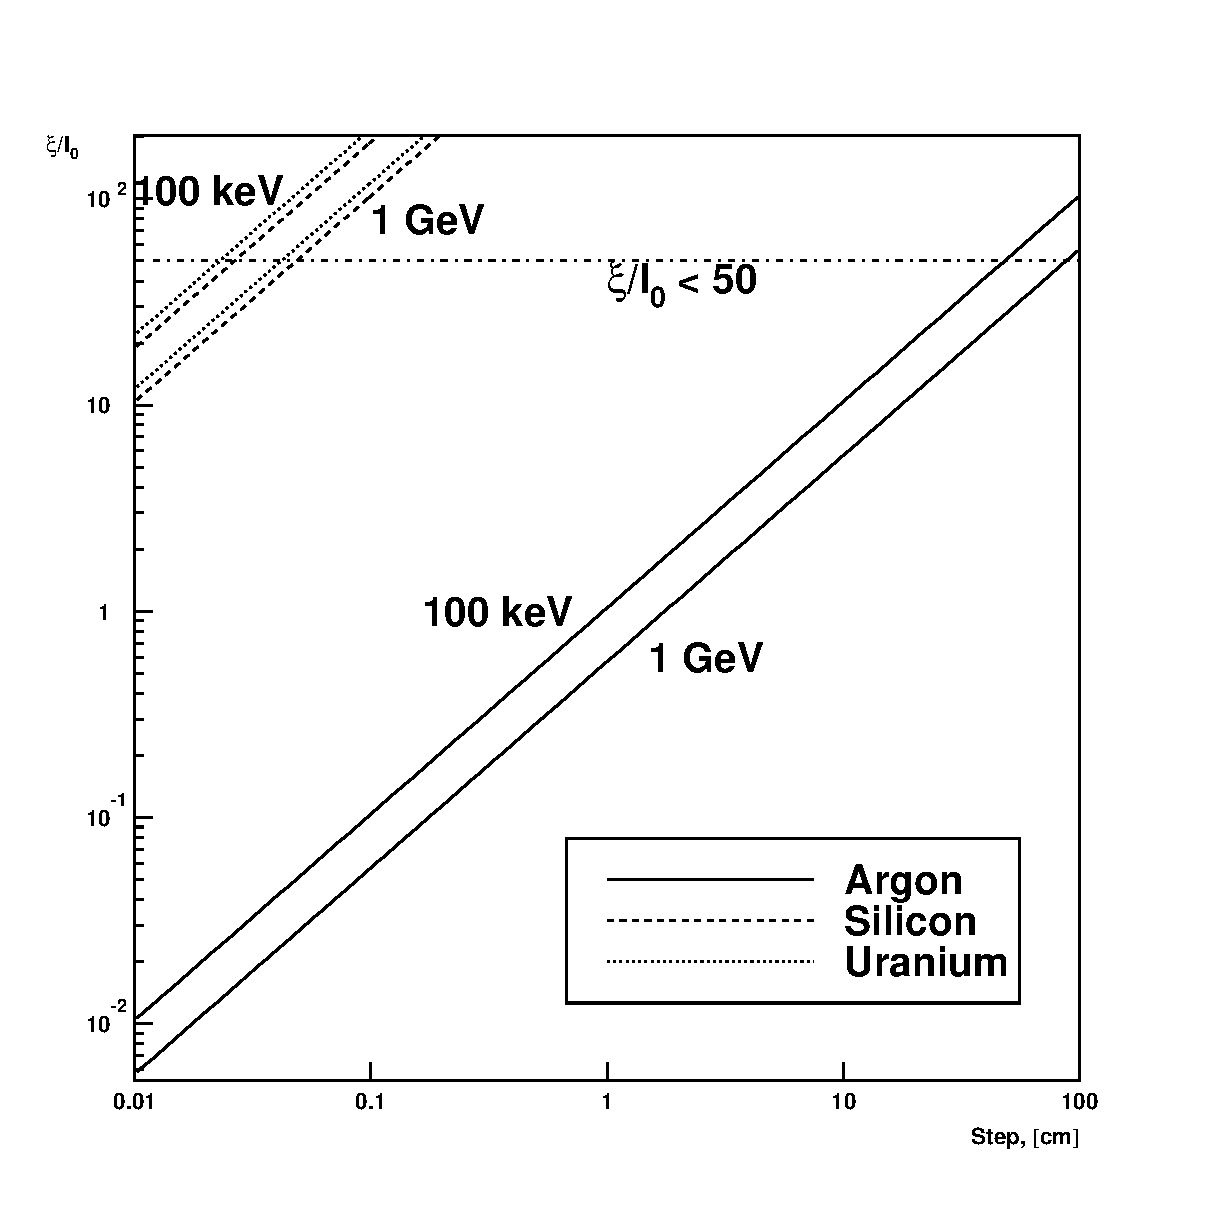
\epsfig{file=eps/phys332-1.eps,width=14cm}
   \caption{The variable $\xi/I_0$ can be used to measure the 
            validity range of the Landau theory. It depends
            on the type and energy of the particle, $Z$, $A$
            and the ionisation potential of the material and
            the layer thickness. 
            }
    \label{fg:phys332-1}
\end{figure}

In the following sections, the different theories and models
for the energy loss fluctuation are described. First, the
Landau theory and its limitations are discussed, and then,
the Vavilov and Gaussian straggling functions and the
methods in the thin layers and gaseous materials are presented.

\subsection{ Landau theory}
\label{sec:phys332-1}
For a particle of mass $m_x$ traversing a thickness of material
$\delta x $,
the Landau probability distribution  may be written in terms of the
universal Landau \cite{bib-LAND}, \cite{bib-KOL3} function $\phi(\lambda)$ as:
\begin{eqnarray*}
f( \epsilon , \delta x ) & = &\frac{1}{\xi} \phi ( \lambda )    
\end{eqnarray*}
where
\begin{eqnarray*}
\phi(\lambda )& = & \frac{1} {2 \pi i}\int^{c+i\infty}_{c-i\infty}
\exp \left ( u \ln u + \lambda u \right ) du \hspace{2cm} c \geq 0 \\
\lambda       & = & \frac{\epsilon  -\bar{\epsilon} }{\xi}
  - \gamma' - \beta^2 - \ln \frac{\xi} {E_{\rm max}}          \\
\gamma' & = & 0.422784\dots = 1 - \gamma \\
\gamma             & = & 0.577215\dots \mbox{(Euler's constant)}   \\
\bar{\epsilon}  & = & \mbox{average energy loss}                    \\
\epsilon      & = & \mbox{actual energy loss}
\end{eqnarray*}

\subsubsection{Restrictions}
The Landau formalism makes two restrictive assumptions :
\begin{enumerate}
\item The typical energy loss is small compared to the maximum energy
loss in a single collision.
This restriction is removed in the Vavilov theory (see section 
\ref{vavref}).
\item
The typical energy loss in the absorber should be large compared
to the binding energy of the most tightly bound electron.
For gaseous detectors, typical energy losses are a few
keV which is comparable to the binding energies of the inner electrons.
In such cases a more sophisticated approach which accounts for atomic
energy levels (see for instance Talman \cite{bib-TALM}) is necessary
to accurately simulate data distributions. In {\tt GEANT}, a parameterised
model by L. Urb\'{a}n is used (see section \ref{urban}).
\end{enumerate}

In addition, the average value of the Landau distribution
is infinite. Summing the Landau fluctuation
obtained to the average energy from the $dE/dx$ tables, we
obtain a value which is larger than the one coming from the table.
The probability to sample a large value is small, so it takes a
large number of steps (extractions) for the average fluctuation to
be significantly larger than zero. This introduces a dependence of the
energy loss on the step size which can affect calculations.

A solution to this has been to introduce a limit on the value of the
variable sampled by the Landau distribution \cite{bib-JONE},
in order to keep the
average fluctuation to 0. The value obtained from the \Rind{GLANDO}
routine is:
\[
\delta dE/dx = \epsilon - \bar{\epsilon} = \xi ( \lambda - \gamma'
+\beta^2 +\ln \frac{\xi}{E_{max}})
\]
In order for this to have average 0, we must impose that:
\[
\bar{\lambda} = -\gamma' - \beta^2 -\ln \frac{\xi}{E_{max}}
\]

This is realised introducing a $\lambda_{max}(\bar{\lambda})$ such that
if only values of $\lambda \leq \lambda_{max}$ are accepted, the average
value of the distribution is $\bar{\lambda}$.

A parametric fit to the universal Landau distribution has been performed,
with following result:

\[
\lambda_{max} = 0.60715 + 1.1934\bar{\lambda}+(0.67794+0.052382\bar{\lambda})
\exp(0.94753+0.74442\bar{\lambda})
\]

only values smaller than $\lambda_{max}$ are accepted, otherwise the
distribution is resampled.



\subsection{Vavilov theory}
\label{vavref}
Vavilov \cite{bib-VAVI} derived a more accurate straggling
distribution by introducing the kinematic limit on the maximum
transferable energy in a single collision, rather than using
$ E_{max} = \infty $. Using the notations of \cite{bib-SCH1} we can write:
\begin{eqnarray*}
f \left ( \epsilon, \delta s \right ) & = & \frac{1}{\xi} \phi_{v}
\left ( \lambda_{v}, \kappa, \beta^{2} \right )
\end{eqnarray*}
 
where
 
\begin{eqnarray*}
\phi_{v} \left ( \lambda_{v}, \kappa, \beta^{2} \right ) & = &
\frac{1}{2 \pi i} \int^{c+i\infty}_{c-i\infty}\phi \left( s \right ) 
e^{\lambda s} ds \hspace{2cm} c \geq 0 \\
\phi \left ( s \right ) & = & 
\exp \left [ \kappa ( 1 + \beta^{2}\gamma ) \right ]
~ \exp \left [ \psi \left ( s \right ) \right ], \\
\psi \left ( s \right )  & = & s \ln \kappa + ( s + \beta^{2} \kappa )
\left [ \ln (s/\kappa) + E_{1} (s/\kappa) \right ] - \kappa e^{-s/\kappa}, 
\end{eqnarray*}
and
\begin{eqnarray*}
E_{1}(z) & = & \int^{\infty}_{z} t^{-1} e^{-t} dt 
\mbox{\hspace{1cm} (the exponential integral)} \\
\lambda_v & = & \kappa \left [ \frac{\epsilon - \bar{\epsilon}}{\xi}
- \gamma' - \beta^2 \right]
\end{eqnarray*}
The Vavilov parameters are simply related to the Landau parameter
by $\lambda_L = \lambda_v/\kappa - \ln\kappa $. It can be shown that 
as $\kappa \rightarrow 0$, the distribution of the variable $\lambda_L$ 
approaches that of Landau. For $\kappa \leq 0.01$ the two distributions
are already practically identical. Contrary
to what many textbooks report, the Vavilov distribution {\em
does not} approximate the Landau distribution for small $\kappa$, 
but rather the distribution of
$\lambda_L$ defined above tends to the distribution of the
true $\lambda$ from the Landau density function. 
Thus the routine \Rind{GVAVIV} samples the 
variable $\lambda_L$ rather than $\lambda_v$. 
For $\kappa \geq 10$ the Vavilov distribution tends to a
Gaussian distribution (see next section).
 
\subsection{Gaussian Theory}
 
Various conflicting forms have been proposed for Gaussian straggling
functions, but most of these appear to have little theoretical or
experimental basis.
However, as noted by Schorr \cite{bib-SCH1} it has been demonstrated 
by Seltzer and Berger \cite{bib-SELT}
that for $\kappa \geq 10 $ 
the Vavilov distribution can be replaced by a Gaussian of the form :
\begin{eqnarray*}
f( \epsilon , \delta s)  \approx \frac{1}
{\xi \sqrt{\frac{2 \pi}{\kappa} \left( 1 - \beta^2/2 \right)}}
   \exp \left [ \frac{( \epsilon - \bar{\epsilon} )^2}{2} \frac{\kappa}
   {\xi^2 (1- \beta^2/2)}\right ]
\end{eqnarray*}
thus implying 
\begin{eqnarray*}
\mbox{mean} & = & \bar{\epsilon} \\
\sigma^2   & = & \frac{\xi^2}{\kappa} (1-\beta^2/2) = \xi E_{max} (1-\beta^2/2)
\end{eqnarray*}

\subsection{Urb\'an model}
\label{urban}
The method for computing restricted energy losses
with $\delta$-ray production above given threshold energy in 
{\tt GEANT} is
a Monte Carlo method that can be used
for thin layers.
It is fast and it can be used for any thickness of a medium.
Approaching the limit of the validity of Landau's theory, the loss
distribution approaches smoothly the Landau form as shown in
figure \ref{fg:phys332-2}.
\begin{figure}[hbt]
   \centering
   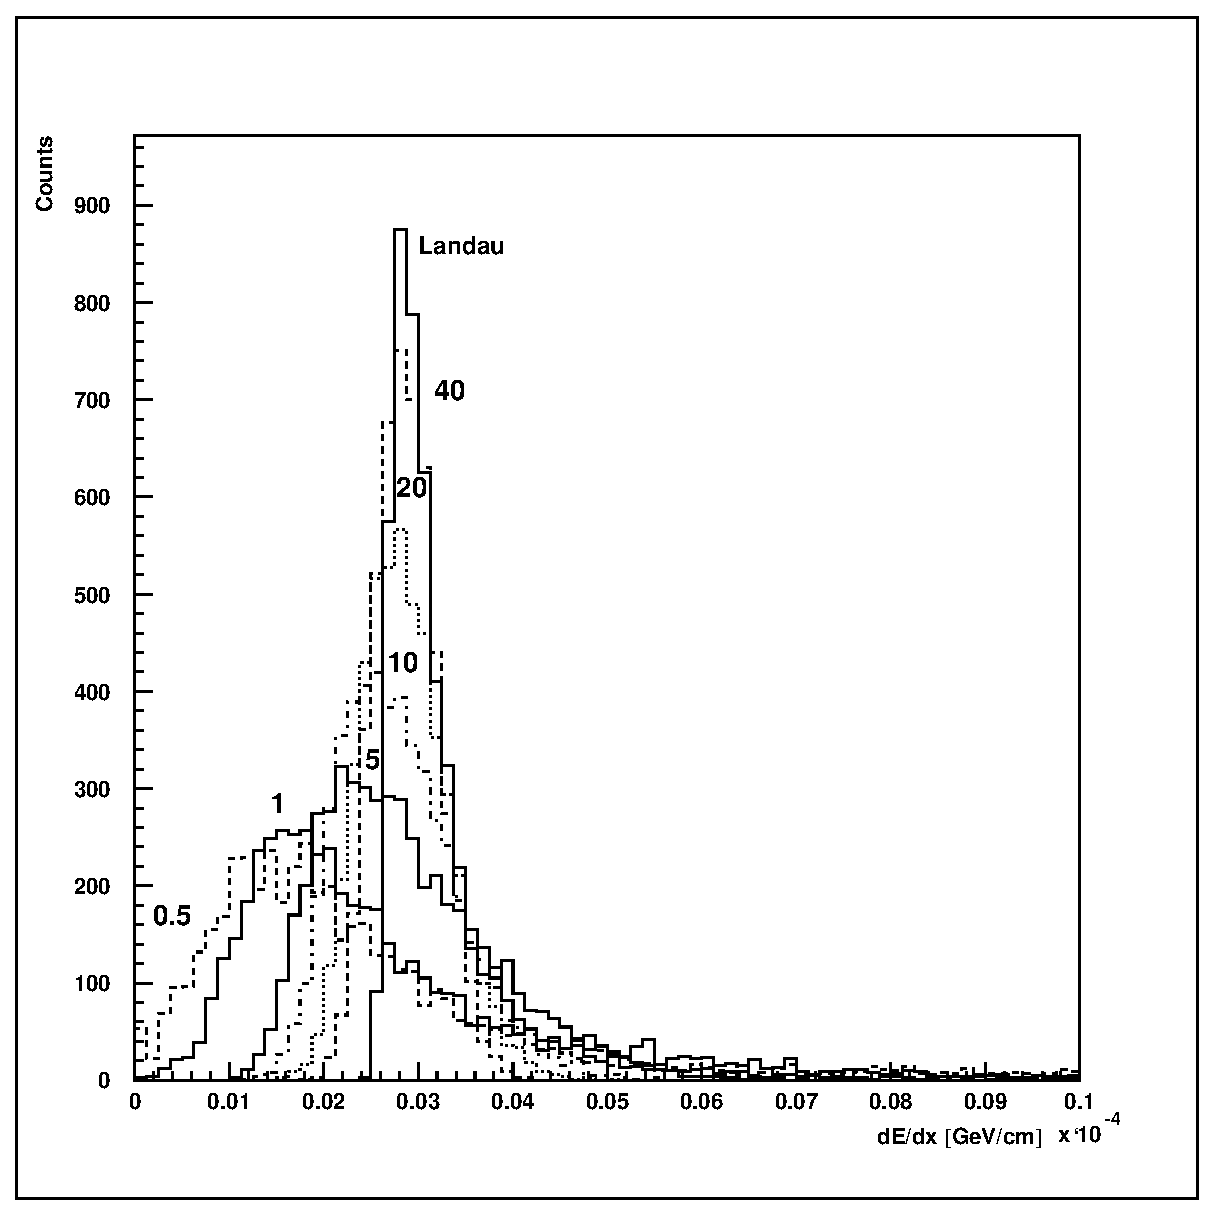
\epsfig{file=eps/phys332-2.eps,width=14cm}
   \caption{Energy loss distribution for a 3 GeV electron in
            Argon as given by standard {\tt GEANT}.
            The width of the layers is given in centimeters.}
    \label{fg:phys332-2}
\end{figure}

It is assumed that the atoms have only two energy levels
with binding energy $E_1$ and $E_2$.
The particle--atom interaction will then be an excitation
with energy loss $E_1$ or $E_2$, or an ionisation
with an energy loss distributed according to a function
$g(E) \sim 1/E^2$:
\begin{equation}
g(E) = \frac{ (E_{max} + I)I}{E_{max}} \frac{1}{E^2}
\end{equation}
The macroscopic cross-section for excitations ($i=1,2$) is
\begin{equation}
\label{eq:sigex}
\Sigma_i = C \frac{f_i}{E_i} \frac{ \ln (2 m \beta^2 \gamma^2/E_i) - \beta^2}
             {\ln (2 m \beta^2 \gamma^2/ I) - \beta^2}(1-r)
\end{equation}
and the macroscopic cross-section for ionisation is
\begin{equation}
\label{eq:sigion}
\Sigma_3 = C \frac{E_{max}}{I(E_{max}+I) \ln(\frac{E_{max}+I}{I})}
           ~ r
\end{equation}
    $E_{max}$ is the {\tt GEANT} cut for $\delta$-production,
    or the maximum energy transfer minus mean
    ionisation energy, if it is smaller than this
    cut-off value.
The following notation is used:

\begin{tabular}{ll}
$r, C$          & parameters of the model \\
$E_i$           & atomic energy levels \\
$I$             & mean ionisation energy \\
${f_i}$         & oscillator strengths \\
\end{tabular}

The model has the parameters $f_i$, $E_i$, $C$ and $r ~(0\leq r\leq 1)$.
The oscillator strengths $f_i$ and the atomic level energies $E_i$ should
satisfy the constraints
\begin{eqnarray}
f_1 + f_2 & = & 1  \label{eq:fisum}\\
f_1 \ln E_1 + f_2 \ln E_2 & = & \ln I \label{eq:flnsum}
\end{eqnarray}
The parameter $C$ can be defined with the help of the
mean energy loss $dE/dx$ in the following way:
The numbers of collisions ($n_i$, i = 1,2 for the excitation and 3 for
the ionisation) follow the Poissonian distribution with a mean
number $ \langle n_i \rangle $. In a step $\Delta x$ the mean number
of collisions is
\begin{equation}
\langle n_i \rangle = \Sigma_i \Delta x
\end{equation}
The mean energy loss $dE/dx$ in a step is the sum of the excitation
and ionisation contributions
\begin{equation}
\frac{dE}{dx} \Delta x = \left[ \Sigma_1 E_1 + \Sigma_2 E_2 +
                          \Sigma_3 \int_{I}^{E_{max}+I} E~g(E)~dE \right]
                         \Delta x
\end{equation}
From this, using the  equations (\ref{eq:sigex}), (\ref{eq:sigion}),
(\ref{eq:fisum}) and (\ref{eq:flnsum}),
one can define the parameter $C$
\begin{equation}
C = \frac{dE}{dx}
\end{equation}

The following values have been chosen in {\tt GEANT} for the other
parameters:

$ \begin{array}{lcl}
f_2 = \left\{ \begin{array}{ll}
             0   & \mbox{if $Z \leq 2$} \\
             2/Z & \mbox{if $Z > 2$} \\
             \end{array} \right.    & \Rightarrow & f_1 = 1 - f_2 \\
E_2 = 10 Z^2 \mbox{ eV}  & \Rightarrow & E_1 = \left(\frac{I}{E_{2}^{f_2}}
                                              \right)^{\frac{1}{f_1}} \\
r  = 0.4 & & \\
\end{array} $

\noindent With these values the atomic level $E_2$ corresponds approximately
the K-shell energy of the atoms and $Zf_2$ the number of K-shell
electrons. $r$ is the only variable which can be tuned freely. It
determines the relative contribution of ionisation and
excitation to the energy loss.

The energy loss is computed with the assumption that the step length
(or the relative energy loss) is small, and --- in consequence ---
the cross-section can be considered constant along the path length.
The energy loss due to the excitation is
\begin{equation}
\Delta E_e = n_1 E_1 + n_2 E_2
\end{equation}
where $n_1$ and $n_2$ are sampled from Poissonian distribution
as discussed above.
The loss due to the ionisation can be generated from the distribution
$g(E)$ by the inverse transformation method:
\begin{eqnarray}
u = F(E) &  = & \int_{I}^E g(x) dx \nonumber \\
E = F^{-1}(u) & = & \frac{I}{1 - u \frac {E_{max}}{E_{max}+I}} \\
\end{eqnarray}
where $u$ is a uniform random number between $F(I)=0$ and $F(E_{max}+I)=1$.
The contribution from the ionisations will be
\begin{equation}
\Delta E_i  = \sum_{j=1}^{n_3} \frac{I}
              {1 - u_j \frac {E_{max}}{E_{max} + I}}
\end{equation}
where $n_3$ is the number of ionisation (sampled from Poissonian
distribution). The energy loss in a step will then be
$\Delta E = \Delta E_e  + \Delta E_i$.

\subsubsection{Fast simulation for $n_3 \geq 16$}
If the number of ionisation $n_3$ is bigger than 16, a faster sampling
method can be used. The possible energy loss interval is divided
in two parts: one in which the number of collisions is large and
the sampling can be done from a Gaussian distribution and the other
in which the energy loss is sampled for each collision.
Let us call the former interval $[I, \alpha I]$ the interval A,
and the latter $[\alpha I,E_{max}]$ the interval B.
$\alpha$ lies between 1 and $E_{max}/I$.
A collision with a loss in the interval A happens with the probability
\begin{equation}
\label{eq:phys332-5}
P(\alpha) = \int_I^{\alpha I} g(\!E\!) \, dE =
            \frac {( E_{max} + I) (\alpha - 1)}{E_{max} \alpha}
\end{equation}
The mean energy loss and the standard deviation for this type
of collision are
\begin{equation}
\langle \Delta E(\alpha) \rangle = \frac{1}{P(\alpha)} 
        \int_I^{\alpha I} E \, g(\!E\!) \, dE =
        \frac{I \alpha \ln \alpha}{\alpha - 1}
\end{equation}
and
\begin{equation}
\sigma^2(\alpha) = \frac{1}{P(\alpha)}
        \int_I^{\alpha I} E^2 \, g(\!E\!) \, dE =
        I^2 \alpha \left( 1 - \frac{\alpha \ln \! ^2 \alpha}{(\alpha - 1)^2} \right)
\end{equation}
If the collision number is high , we assume that the number of the
type A collisions can be calculated from a Gaussian distribution
with the following mean value and standard deviation:
\begin{eqnarray}
\label{eq:phys332-1}
\langle n_A \rangle & = & n_3 P(\alpha) \\
\label{eq:phys332-2}
\sigma_A^2     & = & n_3 P(\alpha) ( 1 - P(\alpha))
\end{eqnarray}
It is further assumed that the energy loss in these collisions
has a Gaussian distribution with
\begin{eqnarray}
\label{eq:phys332-3}
\langle \Delta E_A \rangle & = & n_A  \langle \Delta E(\alpha) \rangle \\
\label{eq:phys332-4}
\sigma_{E,A}^2             & = & n_A \sigma^2(\alpha)
\end{eqnarray}
The energy loss of these collision can then be sampled
from the Gaussian distribution.

The collisions where the energy loss is in the interval B
are sampled directly from
\begin{equation}
\Delta E_B = \sum_{i=1}^{n_3 - n_A} \frac{\alpha I}
            {1 - u_i \frac{E_{max} + I - \alpha I}{E_{max} + I}}
\end{equation}
The total energy loss is the sum of these two types of
collisions:
\begin{equation}
\Delta E =  \Delta E_A + \Delta E_B
\end{equation}

The approximation of equations ((\ref{eq:phys332-1}),  (\ref{eq:phys332-2}),
 (\ref{eq:phys332-3}) and  (\ref{eq:phys332-4}) can be used under
the following conditions:
\begin{eqnarray}
\label{eq:phys332-6}
\langle n_A \rangle - c \, \sigma_A            & \geq & 0 \\
\label{eq:phys332-7}
\langle n_A \rangle + c \, \sigma_A            & \leq & n_3 \\
\label{eq:phys332-8}
\langle \Delta E_A \rangle - c \, \sigma_{E,A} & \geq & 0
\end{eqnarray}
where $c \geq 4$. From the equations (\ref{eq:phys332-5}),
(\ref{eq:phys332-1}) and (\ref{eq:phys332-3}) and from
the conditions (\ref{eq:phys332-6}) and (\ref{eq:phys332-7})
the following limits can be derived:
\begin{equation}
\alpha_{min} = \frac{ (n_3 + c^2)(E_{max}+I)}
                    {n_3 (E_{max} + I) + c^2 I} \; \leq \alpha \; \leq
\alpha_{max} = \frac{ (n_3 + c^2)(E_{max}+I)}
                    {c^2 (E_{max} + I) + n_3 I}
\end{equation}
This conditions gives a lower limit to number of the ionisations $n_3$
for which the fast sampling can be done:
\begin{equation}
n_3 \; \geq \; c^2
\end{equation}
As in the conditions (\ref{eq:phys332-6}), (\ref{eq:phys332-7})
and (\ref{eq:phys332-8}) the value of $c$ is as minimum 4, one gets
$n_3 \; \geq 16$. In order to speed the simulation, the
maximum value is used for $\alpha$.

The number of collisions with energy loss in the interval B
(the number of interactions which has to be simulated
directly) increases slowly with the total number
of collisions $n_3$. The maximum number of these collisions
can be estimated as
\begin{equation}
n_{B,max} = n_3 - n_{A,min} \approx n_3 (\langle n_A \rangle 
            - \sigma_A)
\end{equation}
From the previous expressions for $\langle n_A \rangle$ and
$\sigma_A$ one can derive the condition
\begin{equation}
n_B \; \leq \; n_{B,max} = \frac{2 n_3 c^2}{n_3+c^2}
\end{equation}
The following values are obtained with $c=4$:

\begin{tabular}{llcrr}
$n_3$  & $n_{B,max}$ & & $n_3$  & $n_{B,max}$\\ \hline
16   & 16      & & 200  & 29.63\\
20   & 17.78   & & 500  & 31.01 \\
50   & 24.24   & & 1000 & 31.50 \\
100  & 27.59   & & $\infty$ & 32.00
\end{tabular}
\subsubsection{Special sampling for lower part of the spectrum}
If the step length is very small ($\leq 5$ mm in gases, $\leq$ 2-3 $\mu$m
in solids) the model gives 0 energy loss for some events.
To avoid this, the probability of 0 energy loss is computed
\begin{equation}
P( \Delta E=0) = e^{-( \langle n_1 \rangle + \langle n_2 \rangle
                     + \langle n_3 \rangle )}
\end{equation}
If the probability is bigger than 0.01 a special sampling is done,
taking into account the fact that in these cases the projectile
interacts only with the outer electrons of the atom.
An energy level $E_0 = 10$ eV is chosen to correspond to the
outer electrons. The mean number of collisions can be calculated
from 
\begin{equation}
\langle n \rangle = \frac{1}{E_0} \frac{ dE}{dx} \Delta x
\end{equation}
The number of collisions $n$ is sampled from Poissonian
distribution. In the case of the thin layers, all the
collisions are considered as ionisations and the energy loss
is computed as
\begin{equation}
\Delta E = \sum_{i=1}^n \frac{E_0}
          { 1 - \frac {E_{max}}{E_{max} + E_0} u_i}
\end{equation}


\section{Implementation}

The method to be used for energy loss straggling
is chosen in {\tt GFLUCT}. 
If $\delta$-rays are produced ({\tt DRAY = 1})
above the cut value {\tt DCUTE}
and the detailed PAI simulation for straggling 
in thin layers (see PHYS334)
is not chosen ({\tt STRA = 0}, default),
{\tt GLANDZ} is called always as it samples
from the restricted distribution (the energy
loss of the $\delta$-rays which are explicitly
produced should not be taken into the energy
loss distribution).

If $\delta$-rays are not produced, the
values of $\kappa$ and $\xi /I$ are computed,
and Urb\'an, Landau, Vavilov or Gaussian model
is chosen accordingly.
If Urb\'an model is used, {\tt GLANDZ} will be
called with infinite ({\tt BIG}) value for
the $\delta$-ray production.

When Landau model is chosen, it is possible to use a routine from 
the CERN Program Library to sample
random numbers from the Landau distribution :
\Rind{GENLAN} written by James and Hancock \cite{bib-JAME} and copied 
into {\tt GEANT} source file as \Rind{GLANDG}. This routine has been modified
in order to reproduce the tail for large values of X. The original routine
did not give values of X larger than 200.
\begin{verbatim}
      CALL GENLAN(X)
\end{verbatim}
It should be noted that over the years considerable confusion has
arisen over the precise form and features of the Landau distribution.
As an example, a {\it simpler form} of $\phi(\lambda)$ had been
proposed by Moyal~\cite{bib-MOYA} and
used on occasions which has little in common with
the function defined in section \ref{sec:phys332-1} \cite{bib-KOL2}.

For the Vavilov distribution we have used the function \Rind{GVAVIV}
by Rotondi and Montagna \cite{bib-ROTO}. 

%%%%%%%%%%%%%%%%%%%%%%%%%%%%%%%%%%%%%%%%%%%%%%%%%%%%%%%%%%%%%%%%%%%
%                                                                 %
%  GEANT manual in LaTeX form                                     %
%                                                                 %
%  Michel Goossens (for translation into LaTeX)                   %
%  Version 1.00                                                   %
%  Last Mod. Jan 24 1991  1300   MG + IB                          %
%                                                                 %
%%%%%%%%%%%%%%%%%%%%%%%%%%%%%%%%%%%%%%%%%%%%%%%%%%%%%%%%%%%%%%%%%%%
\Origin{M.Maire}
\Revision{F.Carminati}
\Version{Geant 3.16}\Routid{PHYS333}
\Submitted {30.05.86}\Revised{16.12.93}
\Makehead {Information about energy loss fluctuations}
\section{Subroutines}
\Shubr{GDRPRT}{(IPART,IMATE,STEP,NPOINT)}
\begin{DLtt}{MMMMMMMMMM}
\item[IPART] ({\tt INTEGER}) {\tt GEANT} particle number;
\item[IMATE] ({\tt INTEGER}) {\tt GEANT} material number;
\item[STEP]  ({\tt REAL}) step in cm;
\item[NPOINT] ({\tt INTEGER}) number of logarithmically spaced energy points
between {\tt EKMIN} (default 10 keV) and {\tt EKMAX} (default 10 TeV). See
{\tt [BASE040]} for more information on these value and how to change them
with the {\tt ERAN} input record;
\end{DLtt}

This routine calculates and prints the relevant parameters
relative to the simulation of energy loss fluctuations due to ionisation and
$\delta$-ray production in {\tt STEP} cm:
\begin{DLtt}{MMMMMMMM}
\item[N d-rays] average number of $\delta$-rays produced;
\item[dE/I] average energy loss divided by the
average ionisation potential;
\item[xi/I] variable $\xi/I$ of the Landau/Vavilov
theory;
\item[xi/Emax] variable $\xi/E_{Max}$ of the Landau/Vavilov
theory;
\item[regime] valid model to simulate energy loss fluctuations.
Possible values are:
\begin{DLtt}{MMMMMMMM}
\item[Gauss] Gauss distribution;
\item[Vavilov] Vavilov distribution;
\item[Landau] Landau distribution;
\item[Urb\'{a}n] \Rind{GLANDZ} routine of Urban (see {\tt [PHYS332]});
\item[ASHO] atomic harmonic oscillator approximation (see {\tt [PHYS334]});
\item[PAI]  Photo-Absorption Ionisation model (see {\tt [PHYS334]});
\end{DLtt}
\end{DLtt}

This routine has no action on the {\tt GEANT} 
system. It is intended as a help to users understanding the
model which {\tt GEANT} may be asked to use, 
for instance via the routine \Rind{GSTPAR} {\tt [CONS210]}.

\section{Method}
When a charged particle traverses a portion of matter, 
it interacts with the electrons
and the nuclei of the atoms. Most of 
these interactions are
electromagnetic (quasi-)
elastic collisions in which the incoming particle loses energy in the
laboratory reference frame. The amount of energy loss in a thickness of 
material
$t$ is subject to two sources of fluctuations. The {\it number} of
collisions can fluctuate, and at the same time the {\it energy} lost in each
collision varies statistically. Both distributions are characterised
by a Poissonian-like behaviour. We can distinguish between collisions
where the energy transferred to the atomic electrons is enough to 
extract them from the atoms (ionisation with production of $\delta$-rays)
and collisions where the atomic structure is excited, without a complete
ionisation (excitation). It has to be noted that the energy
transferred to the nuclei is usually negligible. Momentum conservation
considerations show that the ratio of the energy transferred to 
electrons to the energy transferred to nucleus in Coulomb interactions
is of the order of $m_{e}Z A^{-1}m_{p}^{-1}$.

Several theories have been proposed to describe
this important mechanism in the transport of charged particles.
The main difference of these theories is in the greater or lesser
detail with which the scattering centres are described. 
The detail of these theories as they are implemented in {\tt GEANT} can
be found in {\tt [PHYS332]}, {\tt [PHYS334]} for energy loss fluctuations
and in {\tt [PHYS430]}, {\tt [PHYS431]} for energy loss.

In general, the greater the thickness of the layer traversed
in terms of the number of atoms encountered, the larger
is the number of collisions. In this case a detailed description of
the atomic structure may be irrelevant to account for the form of the
fluctuation. Landau and Vavilov have proposed theories in this region
and these are implemented in {\tt GEANT}. 

When the thickness of the material is such that the number of collisions
becomes smaller, the detailed nature of the atomic structure becomes 
important in determining the fluctuations of the energy loss. In this
case the coupling of the various atomic energy levels to the to the
Coulomb field must be taken into account.

When simulating the energy loss by ionisation, the average path-length
between collisions is a function of the cross section $\sigma(E)$.
This cross section becomes very large
when $E \rightarrow 0$, so that it is necessary
to establish a threshold energy below which the process is described in a
{\it condensed} way. Above this threshold, ionisations are
described in a detailed way, with the production of $\delta$-rays.
Thus, when a charged particle is moving in a medium, there are
in general two ways to simulate the energy loss by ionisation:
\begin{enumerate}
\item calculate the average value the energy loss 
via the full Bethe-Bloch equation. This takes into account
$\delta$-rays generation. The fluctuations are then explicitly
introduced via an appropriate distribution.
In {\tt GEANT} 
this method is selected by the value {\tt ILOSS = 2} which is
controlled by the {\tt LOSS} data record.
\item explicitly generate the $\delta$-rays {\it above} a given 
threshold ({\tt DCUTE} for electrons, {\tt DCUTM} for others particle).
In this case the average energy
loss is computed from a restricted formula and
both the value of the energy loss
and the number of $\delta$-rays
produced are function of the threshold cut (hereafter {\tt DRCUT}).
In {\tt GEANT} this method is selected by the value {\tt ILOSS = 1} which is
controlled by the {\tt LOSS} data record.
\end{enumerate}

\subsection{Validity ranges for the different models}
The limits of the validity for
the various models are somewhat arbitrary
within a certain range of material densities and particle energies.
To help determine these limits, some characteristic parameters are used:

\begin{DLtt}{MMMMMMMMMMMMM}
\item[$\xi$] typical energy loss of
a particle in a given layer of material. Its value is:

\[
\xi = 2 \pi r_{e}^{2} m_{e} c^{2} N_{Av} \left ( \frac{Z_{inc}}
{\beta} \right )^{2} \frac{Z \rho t}{A} = 0.1535 \left ( \frac{Z_{inc}}
{\beta} \right )^{2} \frac{Z \rho t}{A} \: (MeV)
\]

\item[$E_{Max}$] maximum transferable energy in a single collision:

\[
E_{Max} = \frac{2 m_{e} \beta^{2} \gamma^{2}}{1 +2 \gamma \frac{m_{e}}
{M} +\left ( \frac{m_{e}}{M} \right ) ^{2}}
\]

where $M$ is the mass of the incoming particle. Note that for incoming
electrons this value has to be divided by 2 due to the impossibility
distinguishing the two electrons in the final state.

\item[$I$] typical electron binding energy. This is a value which 
characterises the average energy levels of the atomic electrons. In
{\tt GEANT} it is parametrised as:

\[
I = 16 Z^{0.9} \: (eV)
\]

\item[$\displaystyle \frac{dE}{dx} \: t$] 
average energy loss by the particle in a
layer of thickness $t$ according to the {\tt GEANT} energy loss tables.

\item[$\xi/E_{Max}$] (hereafter $\kappa$) 
relative importance of high energy transfer collisions 
in the ionisation process

\item[$\min \left ( \frac{dE}{dx} \: t,\xi \right )/I$] 
(hereafter $\Delta$) estimation of the number of collisions
with energy close to the ionisation energy.
\end{DLtt}

In {\tt GEANT} two variables control the model used to describe the
energy loss fluctuations: 
\begin{DLtt}{MMMMMMMMMM}
\item[ILOSS] fluctuation model:
\begin{DLtt}{MMMMM}
\item[0] no energy loss;
\item[1] $\delta$-rays are produced above the threshold,
{\it reduced}
fluctuations from $\delta$-rays below the threshold are added to the
energy loss;
\item[2] no $\delta$-rays are produced, complete fluctuations are calculated;
\item[3] same as {\tt 1};
\item[4] no fluctuations;
\end{DLtt}
\item[ISTRA] energy loss model for {\it thin} layer (see below):
\begin{DLtt}{MMMMM}
\item[0] Urb\'{a}n model;
\item[1] PAI model;
\item[2] ASHO model for $1 < \Delta \leq 30$,(not yet available) 
PAI model otherwise;
\end{DLtt}
\end{DLtt}
The validity limits of the different models are estimated
as follows:
\begin{enumerate}
\item {\bf large number of low-energy collisions: $\Delta \geq 50$}

if $\delta$-rays generation is requested ({\tt ILOSS = 1} or {\tt 3} and 
{\tt IDRAY = 1}) the Urb\'{a}n model is used. If $\delta$-rays are not
produced ({\tt ILOSS = 2} and {\tt IDRAY = 0}) we distinguish three regions:
\begin{enumerate}
\item {\bf very few energy transfers close to the 
maximum: $\kappa \leq 10^{-2}$}

the Landau distribution is used;

\item {\bf few energy transfers close to the 
maximum: $10^{-2} < \kappa \leq 10$}

the Vavilov distribution is used;

\item {\bf many energy transfers close to the 
maximum: $\kappa > 10$}

the Gauss distribution is used;

\end{enumerate}

\item {\bf small number of low-energy collisions: $ \Delta < 50$}

in this region the same model is used for $1 \leq \mbox{\tt ILOSS}
\leq 3$ irrespective of the value of {\tt IDRAY}.
The model used depends on the value of {\tt ISTRA}.

\begin{enumerate}
\item {\bf $ 30 < \Delta \leq 50$}

Urb\'{a}n model if {\tt ISTRA} $= 0$, PAI model otherwise.

\item {\bf $ 1 < \Delta \leq 30$}

Urb\'{a}n model if {\tt ISTRA} $= 0$, PAI model if {\tt ISTRA}
$=1$ and ASHO model if {\tt ISTRA} $=2$.

\item {\bf $ 0.01 < \Delta \leq 1$}

Urb\'{a}n model if {\tt ISTRA} $= 0$, PAI model otherwise.

\item {\bf $ \Delta \leq 0.01$}

Urb\'{a}n model if {\tt ISTRA} $=0$, PAI model otherwise.

\end{enumerate}
\end{enumerate}

\subsection{Recommendations}
The full energy loss fluctuations or the restricted fluctuations
complemented by the production of $\delta$-rays give equivalent
results if the number of $\delta$-rays generated 
is sufficient, e.g. a few tens along
the full trajectory of the particle in the medium.
 
For a relativistic particle, the number of delta-rays
produced per cm can be estimated integrating the
cross section provided in~\cite{bib-PDGB}:
\begin{equation}
\frac{dN}{dx} \approx \frac{D}{2} \frac{\rho Z}{A} 
\frac{Z_{inc}^2}{\mbox{\tt DRCUT}}
\end{equation}
where
\begin{DLtt}{MMMMMMM}
\item[$D$] 0.307 MeV cm$^2$ g$^{-1}$;
\item[$\rho$] density of the medium;
\item[$Z,A$] atomic number and atomic weight of the medium;
\item[$Z_{inc}$] charge of the particle;
\item[DRCUT] energy threshold for emitted delta-rays.
\end{DLtt}
This formula holds for electrons/positrons as well as for other particles.
The number of $\delta$-rays must be sufficient 
to reproduce the statistical fluctuations in the energy loss,
but not too large, as in this case
a large amount of time could be spent in 
tracking them
without a corresponding improvement of the energy loss distribution.

On the other hand, the distribution of the
energy {\it lost} by a particle does not necessarily correspond to the
distribution of the energy {\it deposited} by the same particle in the
medium traversed. This is particularly true for light or {\it thin}
materials where $\delta$-rays can escape into the
next material.

It is the responsibility of the user to estimate the number of $\delta$-rays 
per cm that are needed, according to the considerations above. Then the 
correct value for {\tt DRCUT} should be set with the help of \Rind{GDRPRT}. 
It is recommended to use the same value for {\tt DCUTE} and {\tt DCUTM}.
As the {\tt GEANT} tables for cross-sections are not generated below 
{\tt EKMIN}, {\tt DRCUT} cannot be smaller than {\tt EKMIN}. The value of 
{\tt EKMIN} can be changed via the {\tt ERAN} data record, and its default
value is $10$ keV.

In a {\it light} material like gas, the number of emitted $\delta$-rays for
{\tt DRCUT} $=10$ keV may not be sufficient to ensure a correct energy loss 
distribution. If the user is mainly interested in the energy lost by the 
particle, no discrete $\delta$-ray should be produced setting {\tt ILOSS} 
$=2$ (see {\tt [PHYS332]}).

In case the user is more interested in a precise simulation of the energy 
deposited, then the explicit $\delta$-ray generation should be tried.

As far as {\it thin} materials are concerned ($\Delta < 50$), the default
in {\tt GEANT} is to use the Urb\'{a}n model. Comparison with experimental
data have shown that this model gives very good results, and it is
considerably faster than both the ASHO and the PAI models. Users should
understand well their setup and their results before they try with
different models, which, in principle, should give very similar results.

\subsection{Default values in {\tt GEANT}}
 
In order to avoid double counting, there is an automatic protection in
the code:
{\it if {\tt ILOSS=2}, {\tt IDRAY} is set to 0 and the generation of 
$\delta$-rays is disabled}.
 
The following table summarises the different cases:
\begin{center}
\begin{tabular}{|c|c|c|}\hline
                    &\tt LOSS=2          &\tt LOSS=1     \\
                    &(default)            &               \\
                    \cline{2-3}
     \tt IDRAY      & 0                   &     1          \\
     \tt DCUTE      &  $10^4$ GeV         & \tt CUTELE     \\
     \tt DCUTM      &  $10^4$ GeV         & \tt CUTELE     \\
\hline
\end{tabular}
\end{center}
Where {\tt LOSS}$=1$ means that the restricted fluctuation is 
activated and {\tt LOSS}$=2$ means that the complete Landau/Vavilov/Gauss
fluctuations are used in the region $\Delta \geq 50$. 

%%%%%%%%%%%%%%%%%%%%%%%%%%%%%%%%%%%%%%%%%%%%%%%%%%%%%%%%%%%%%%%%%%%
%                                                                 %
%  GEANT manual in LaTeX form                                     %
%                                                                 %
%  Michel Goossens (for translation into LaTeX)                   %
%  Version 1.00                                                   %
%  Last Mod. Jan 24 1991  1300   MG + IB                          %
%                                                                 %
%%%%%%%%%%%%%%%%%%%%%%%%%%%%%%%%%%%%%%%%%%%%%%%%%%%%%%%%%%%%%%%%%%%
\Origin{I.Gavrilenko, P.Nevski, K.Lassila-Perini}
\Documentation{K.Lassila-Perini}
\Version{Geant 3.21}\Routid{PHYS334}
\Submitted {11.03.94}\Revised{11.03.94}
\Makehead {Models for energy loss fluctuations in thin layers}

\section{Subroutines}

\Shubr{GSTINI}{}
\Rind{GSTINI} initializes the tables that are used for sampling of
the energy loss, if the user has set the flag {\tt STRA = 1}.
It calls the subroutine \Rind{GSTXIN} to integrate
an expression for the number of collisions and \Rind{GSTTAB}
for preparing the tables for different Lorentz factors.
It is called from \Rind{GPHYSI} at initialization time.

\Shubr{GSTXIN}{}
\Rind{GSTXIN} computes the values needed for the sampling tables.
It uses the functions \Rind{GOSCIN} to integrate over the
photoelectric cross-sections and the function \Rind{GKOKRI}
to compute the real part of the complex dielectric constant.
\Rind{GSTXIN} is called from \Rind{GSTINI}.

\Sfunc{GOSCIN}{VALUE = GOSCIN(EIN1EV,EIN2EV)}
\Rind{GOSCIN} integrates the parameterization of the photoelectric
cross-sections from energy {\tt EIN1EV} to energy {\tt EIN2EV}.
It is called from \Rind{GSTXIN}.

\Sfunc{GKOKRI}{VALUE = GKOKRI(E,EMINEV,EMAXEV)}
\Rind{GKOKRI} computes the real part of the complex dieletric
constant which is needed in the preparation of energy loss
sampling tables. {\tt E} in the energy for which the values
are being tabulated, {\tt EMINEV} and {\tt EMAXEV} are
the integration limits. \Rind{GKOKRI} is called from
\Rind{GSTXIN}.

\Shubr{GSTTAB}{(GAM,NT,EN,FN)}
\Rind{GSTTAB} prepares the energy loss sampling tables for
different Lorentz factors. The input {\tt GAM} is the Lorentz factor,
the output values are: {\tt NT} the lenght of the table,
{\tt EN} the energy array and {\tt FN} the cumulative probabilty array.
It calls \Rind{GXGINT} to integrate over the probability
function \Rind{GSTDN} to
get the value of {\tt FN}. \Rind{GSTTAB} is called from
\Rind{GSTINI}.

\Sfunc{GXGINT}{VALUE = GXGINT(EXT,A,B,EPS)}
\Rind{GXGINT} performs the Gaussian integration from {\tt A} to
{\tt B} over the function {\tt EXT} with accuracy {\tt EPS}.
It is called from \Rind{GSTTAB} to integrate over the probability
function \Rind{GSTDN}.

\Sfunc{GSTDN}{VALUE = GSTDN(LGE)}
\Rind{GSTDN} is the function which gives the probability for a collision
with energy transfer {\tt LGE}. It is integrated to get the
cumulative probabilty function to be used in the sampling
of the energy loss.

\Shubr{GSTREN}{(GAMMA,ECUT,STEP)}
\Rind{GSTREN} computes the energy loss for a particle of
Lorentz factor {\tt GAMMA} in a step of length {\tt STEP}
if the user has set the flag {\tt STRA = 1}.
{\tt ECUT} is the cut for the $\delta$-ray production.
\Rind{GSTREN} is called from \Rind{GFLUCT}.

\section{The method}
In thin layers, the Landau model of energy loss fluctuations
is not valid, because the number of collisions is too small.
In this case, the atomic structure of the atom has to be
taken into account. The photoabsorption ionization
(PAI) model uses the photoelectric cross-sections
to describe the energy loss distribution.
The results (the width and the most probable value of
the energy loss distribution function)
given by this model are equal to those given by
standard {\tt GEANT} procedure described in {\tt [PHYS332]}.
In addition, however, it gives an estimate of the number
of collision in each step ({\tt NICOLL} in the common block
{\tt GCSTRA}). PAI model is slower than the standard
{\tt GEANT} method.

PAI model is activated, if the user set the flag
{\tt STRA = 1}. The default value is 0.

\subsection{The photoabsorption ionization model}
An expression for the distribution of energy loss can be derived
considering the energy loss as the sum of the energy transfers in
the electromagnetic interactions between
the particle and the atom.
As the interaction is small (i.e. the energy transfer is
small compared to the energy of the passing particle),
Born approximation can be used in the perturbation theory.
In the derivation, the atomic transition current is
considered as a sum of the transition currents of its
electrons.


$\varepsilon$ is the complex
dielectric constant of a medium which describes the
electromagnetic properties of
the medium and thus the effect of the field of an atom
on the energy loss of the particle.

The complex dielectric constant can be written $\varepsilon =
\varepsilon_1 + i \varepsilon_2$ where $\varepsilon_1$ describes
the polarization and $\varepsilon_2$ the absorptive properties
of the medium. $\varepsilon_2$ can be expressed with the
help of the oscillator strength function $f(k,\omega)$ which
describes the coupling of the electrons to the field of the
atom.
\begin{equation}
\label{eps2}
\varepsilon_2 = \frac{2 \pi^2 N e^2}{m \omega} f(k,\omega)
\end{equation}
$m$ is the mass of the electron and $N$ is the electron density.
In a simplified model, the photoabsorption cross-section
$\sigma_{\gamma}(\omega)$ can be used for description of $f(k,\omega)$:
\begin{equation}
f(k,\omega) = \frac{mc}{2\pi^2 e^2 Z} \sigma_{\gamma}(\omega)
\end{equation}
$Z$ being the atomic number of the medium.
The real part of $\varepsilon$ can be  expressed as an integral
of the imaginary part according to the Kronig's and Kramers' dispersion
relation\cite{bib-ALLIS}:
\begin{eqnarray}
\varepsilon_1 - 1 & = & \frac{2}{\pi} P \int_0^{\infty}
     \frac{x \varepsilon_2(x) dx}{x^2 - \omega^2} \nonumber \\
                  & = & \frac{2 N c}{\pi Z} P \int_0^{\infty}
     \frac{\sigma_{\gamma}(x) dx}{x^2 - \omega^2}
\label{eps1}
\end{eqnarray}
where $P$ indicates the Cauchy principal value.
Using these assumptions for the interaction between the projectile
and the atom, the
following form is obtained for the collision cross-section \cite{bib-GRISH}:
\begin{eqnarray}
\frac{d\sigma}{dE}     & = & - \frac{e^2}{\pi \hbar^2c^2n_a}
    \mbox{ Im} \left[ \left( \frac{1}{\beta^2\varepsilon} - 1 \right)
              \ln \frac{2mv^2}{E(1-\beta^2\varepsilon)} \right] \nonumber \\
& &  + \frac{2\pi Ze^4}{mv^2E^2} \int_0^{\infty}
    \frac{f(E')}{\varepsilon(E')^2} dE'
\label{xsection}
\end{eqnarray}
where $n_a$ is the number of atoms per cm$^3$, $v$ velocity of the particle,
and $\beta=v/c$. The number of collisions per distance $x$ and
the energy $E$ is then
\begin{equation}
\frac{N^2}{dx dE} = n_a \frac{d\sigma}{dE}
\end{equation}

For the simulation purposes, the number of primary collisions
in a unit length
with energy loss greater than a certain E
is computed and tabulated for several values of the Lorentz factor.
This is done by integrating
\begin{eqnarray}
\left( \frac{dN}{dx} \right)_{>E}
& = &\int_E^{E_{max}} n_a \frac{d\sigma}{dE} dE
\label{integ}
\end{eqnarray}

\subsection{Implementation}
A photoabsorption ionization Monte Carlo code provided to us by users
%\cite{trd}
has been implemented in {\sc GEANT}. Tables are
prepared at initialization time and sampling from these
tables is done each step at running time. An important
thing to note is the dependence of the $(dN/dx)_{>E}$
on the photoelectric
cross-sections which, when taken from different sources,
may differ considerably, especially at low energies.

To fill the tables, the integration of equation \ref{xsection}
has to be done.
Before the integration over the energy, the integral
over
the oscillator strength function $f(k,\omega) \sim
\sigma_{\gamma}(\omega)$ (last term in equation \ref{xsection})
and the dielectric constant (equations \ref{eps1} and \ref{eps2})
$\varepsilon$ have to be computed. These integaration
can be done analytically when the parameterized cross-sections
are used.

The oscillator strength function should
fulfill the Bethe sum rule \cite{bib-BETH}:
\begin{equation}
\int_0^{\infty} f(k,\omega) d\omega = 1
\label{sumrule}
\end{equation}
To respect this condition, in the PAI model, one has to add some
contribution from the excitation processes to low-energy region
of the photoelectric cross-sections \cite{bib-ALLIS}. In {\sc GEANT}, the
photoelectric cross-section
parameterization of the Sandia \cite{bib-SANDIA} report is used.
In order not to change the tabulated parameterization, the sum
rule is taken into account by lowering the energy
limit for the integration below the ionization limit.
This will not satisy the equation \ref{sumrule} in all cases.
In the program, however, the Bethe sum rule is forced by
dividing the integrated cross-section from $E$ to $\infty$
by the value given by the integration over the whole range.
\begin{figure}[t]
   \centering
   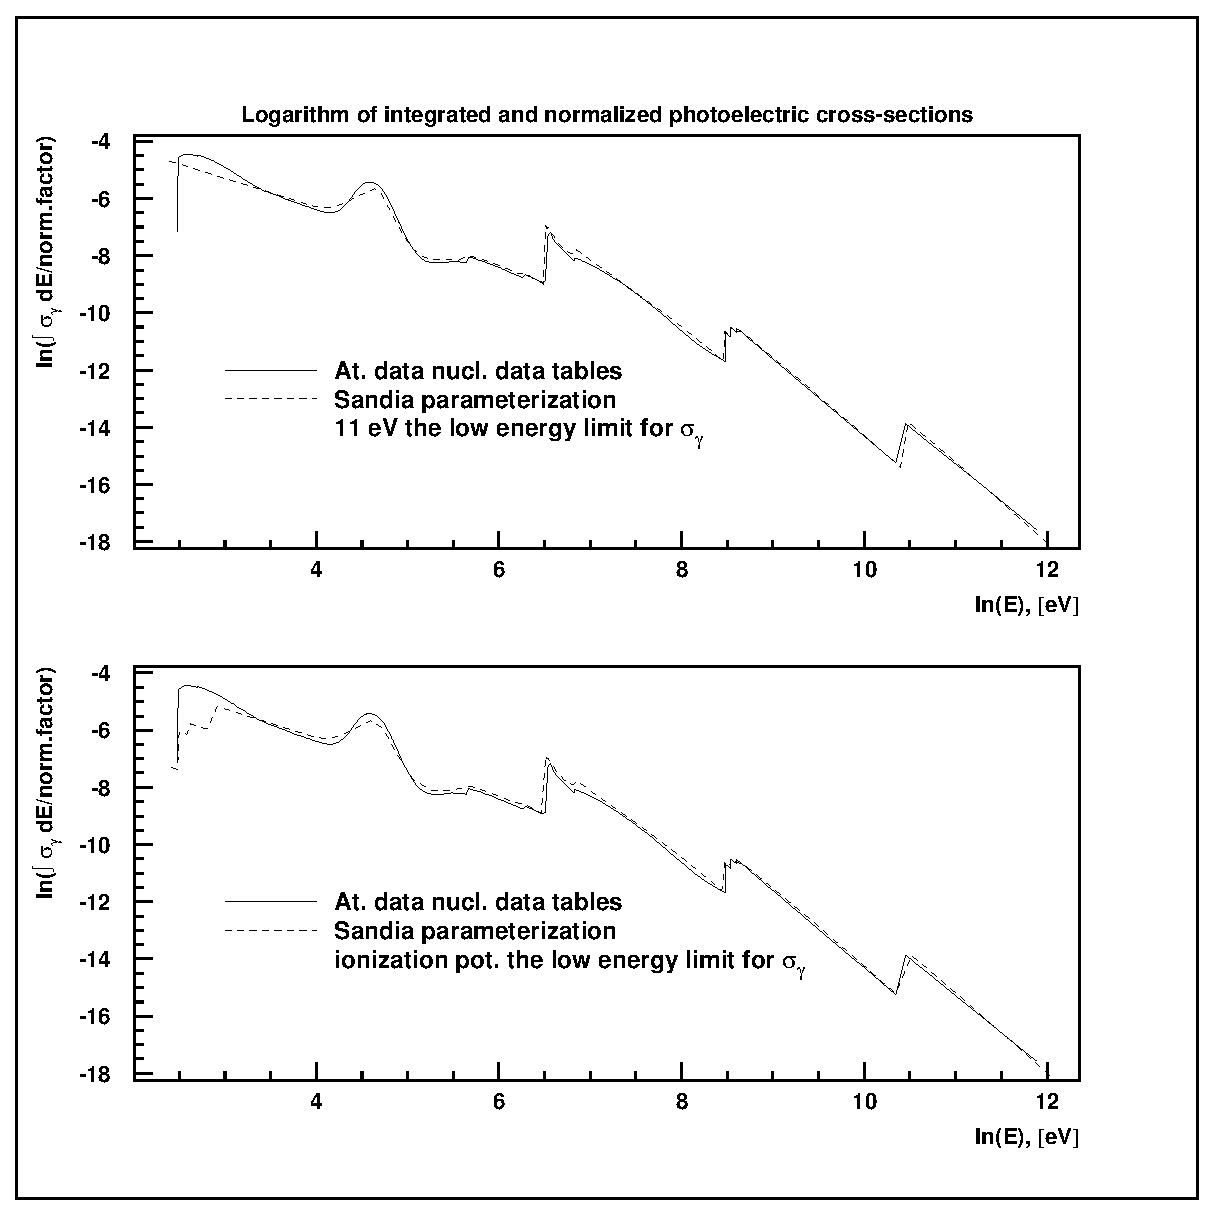
\epsfig{file=eps/phys334-1.eps,width=10cm}
   \caption{Above, the integrated and normalized cross-section
    of the gas mixture 70\% Xe - 10\% CO$_2$ - 20\% CF$_4$
    for two different data sets. The low energy limit
    of the cross-sections from the Sandia data in chosen
    to be 11 eV. In the figure below, the low energy limit
    is the ionization limit for each component of the mixture}
    \label{fosc}
\end{figure}
In figure \ref{fosc}, the integrated cross-section (oscillator
strength function)
$\int_{E}^{E_{max}} \sigma_{\gamma} / \int_{E_0}^{E_{max}} \sigma_{\gamma}$
is given for two different sets of photoelectric cross-section
data for a gas mixture 70\% Xe - 10\% CO$_2$ - 20\% CF$_4$.
In the figure below, the continuous line is the result of the
integration tabulated from \cite{bib-ATOM1} \cite{bib-ATOM2} \cite{bib-ATOM3} 
and the dashed line
is from the integration of {\sc GEANT} cross-sections
considering the lower limit of the cross-section the ionization
energy (12.3 eV for Xe, 11.26 eV for C, 13.6 for O, and
17.42 for F).
In the figure above, the continuous line is as before, but for
the dashed line, the lower limit of the cross-sections is
considered to be 11 eV for all elements of the mixture
to compensate for the sum rule.

The imaginary part of the complex dielectric constant can then
be computed from the integrated cross-section.
To compute the real part of $\varepsilon$, one needs to take the
Cauchy principal value which is basically a limiting process
cancelling the two infinite contribution around the pole
$(x_0-\delta,x_0+\delta)$. The derivation of the real part
with the Sandia parametrization is shown in detail
in the appendix.
\begin{figure}[t]
   \centering
   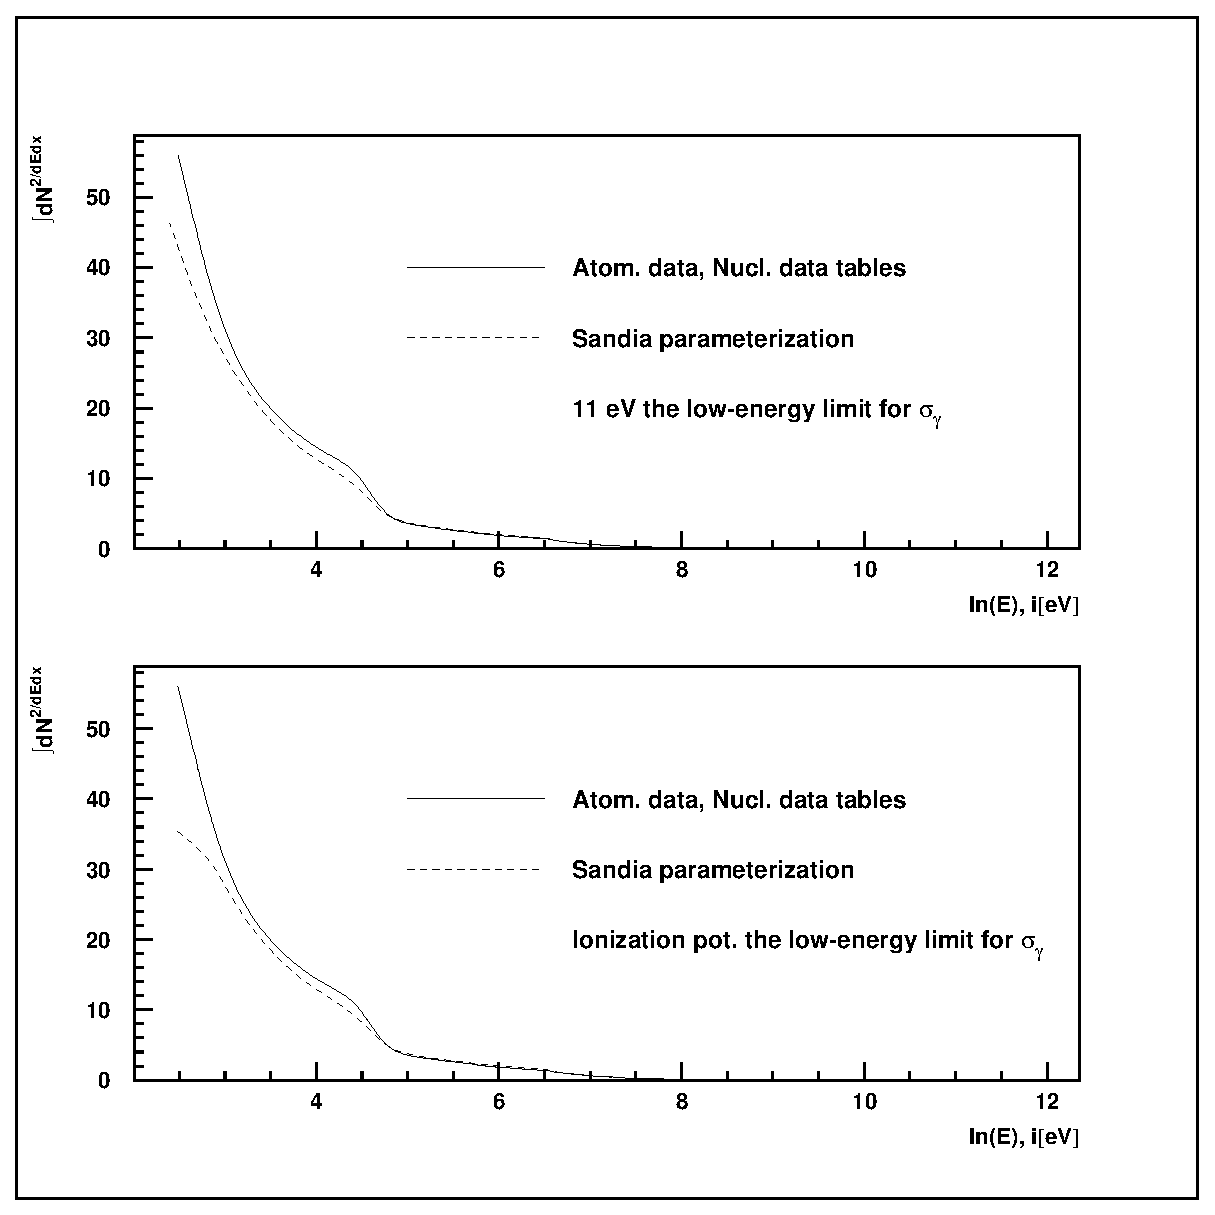
\epsfig{file=eps/phys334-2.eps,width=10cm}
   \caption{Above, the integrated and normalized cross-section
    of the gas mixture 70\% Xe - 10\% CO$_2$ - 20\% CF$_4$
    for two different data sets. The low energy limit
    of the cross-sections from the Sandia data in chosen
    to be 11 eV. In the figure below, the low energy limit
    is the ionization limit for each component of the mixture}
    \label{idndx}
\end{figure}

Knowing the values of complex dielectric constant and the integrated
cross-section, the integration of equation \ref{integ} can
be done. This is done for several values of Lorentz factor
during the initialization time in  subroutine {\tt GSTINI}.
The value of energy loss is sampled from these tables in
subroutine {\tt GSTREN}.

One should remember the dependence of this method on the
photoelectric cross section data.
Figure \ref{idndx} shows the results for the two different
data sets. The difference in the low-energy part is very
significative as the sampling is done from these tables
and, according the inverse transverse method, the number of
collisions is sampled between the maximum and minimum
of the curves in figure \ref{idndx}.









%%%%%%%%%%%%%%%%%%%%%%%%%%%%%%%%%%%%%%%%%%%%%%%%%%%%%%%%%%%%%%%%%%%
%                                                                 %
%  GEANT manual in LaTeX form                                     %
%                                                                 %
%  Michel Goossens (for translation into LaTeX)                   %
%  Version 1.00                                                   %
%  Last Mod. Jan 24 1991  1300   MG + IB                          %
%                                                                 %
%%%%%%%%%%%%%%%%%%%%%%%%%%%%%%%%%%%%%%%%%%%%%%%%%%%%%%%%%%%%%%%%%%%
\Authors {F.Carminati} \Origin{N.Van Eijndhoven}
\Version{Geant 3.16}\Routid{PHYS337}
\Submitted {26.07.93}\Revised{16.12.93}
\Makehead {Birks' saturation law}
\section{Subroutines}
\Shubr{GBIRK}{(EDEP)}

\begin{DLtt}{MMMMMMMM}
\item[EDEP] ({\tt REAL}) and on output the energy
equivalent to the calorimeter response in the current step.
\end{DLtt}

Organic scintillators are usually calibrated with particles whose
energy is near the minimum ionisation ($\gamma \beta \approx 4$).
However, the energy response of such scintillators 
for large local energy deposit is
attenuated. \Rind{GBIRK} returns the energy {\it detected} by
the scintillator in the current step.

\section{Method}

The phenomenological description of the response attenuation of
organic scintillators~\cite{bib-BIRK} is known as Birks' law:
\begin{equation}
R = \frac{\Delta E}{1 + C_1 \delta + C_2 \delta^2} 
\hspace{4cm}
\delta = \frac{1}{\rho} \frac{dE}{dx} \hspace{0.5cm} 
\mbox{MeV g$^{-1}$ cm$^{2}$}
\end{equation}
The values quoted in~\cite{bib-BIR1} for the parameters $C_1, C_2$
are:
\[
C_1 = 0.013 \: \mbox{g MeV$^{-1}$ cm$^{-2}$ \hspace{1.5cm} and \hspace{1.5cm}}
C_2 = 9.6 \times 10^{-6} \: \mbox{g$^{2}$ MeV$^{-2}$ cm$^{-4}$}
\]
These values have been measured for various scintillators.
If the charge of the particle is greater than one, a better description
can be obtained by correcting $C_1$:
\begin{equation}
\label{eq:phys337-1}
C_1' = \frac{7.2}{12.6} C_1 \approx 0.5714 C_1
\end{equation}

The values of the parameters of Birks' formula (if defined) are in the
{\tt ZEBRA} bank next to the material bank:
\begin{DLtt}{MMMMMMMMMMMMMMMMMMMM}
\item[JTM = LQ(JMATE-NTMED)] pointer to the current tracking medium bank;
\item[JTMN = LQ(JTM)] pointer to the {\it next} bank to the current
material one, where the specific tracking medium parameters are stored;
\item[MODEL = Q(JTMN+27)] flag controlling the correction (\ref{eq:phys337-1})
for multiply charged particles:
\begin{DLtt}{MMMM}
\item[$\neq$1] correction is not applied;
\item[$=$1] correction is applied;
\end{DLtt}
\item[C1 = Q(JTMN+28)] first parameter of the Birks' formula;
\item[C2 = Q(JTMN+29)] second parameter of the Birks' formula.
\end{DLtt}
These parameters are set via the \Rind{GSTPAR} routine, with
names {\tt BIRK1}, {\tt BIRK2} and {\tt BIRK3}, respectively. For instance,
to define the standard Birks' parameters for tracking medium {\tt ITM}
with correction for multiply charged particles, one would have to insert
the following piece of code, after the definition of tracking media
but before the call to \Rind{GPHYSI}
\begin{verbatim}
      CALL GSTPAR(ITM,'BIRK1',1.)
      CALL GSTPAR(ITM,'BIRK2',0.013)
      CALL GSTPAR(ITM,'BIRK3',9.6E-6)
\end{verbatim}

%%%%%%%%%%%%%%%%%%%%%%%%%%%%%%%%%%%%%%%%%%%%%%%%%%%%%%%%%%%%%%%%%%%
%                                                                 %
%  GEANT manual in LaTeX form                              %
%                                                                 %
%  Michel Goossens (for translation into LaTeX)                   %
%  Version 1.00                                                   %
%  Last Mod. Jan 24 1991  1300   MG + IB                          %
%                                                                 %
%%%%%%%%%%%%%%%%%%%%%%%%%%%%%%%%%%%%%%%%%%%%%%%%%%%%%%%%%%%%%%%%%%%
\Origin{L. Urb\'{a}n}
\Version{Geant 3.16}\Routid{PHYS340}
\Submitted{28.05.86} \Revised{16.12.93}
\Makehead{Total cross-section and energy loss for bremsstrahlung
by e-e+}

\section{Subroutines}
\Shubr{GBRELA}{}
\Rind{GBRELA} fills the tables for the energy loss of electrons,
positrons and muons due to
bremsstrahlung at initialisation time for different materials.
The energy
binning is set within the array \texttt{ELOW} (common \FCind{/CGMULO/}) in the
routine \Rind{GPHYSI}. In the tables, the dE/dx due to bremsstrahlung
is summed with that due to the ionisation. For energy loss
of electrons and positrons, \Rind{GBRELA} calls the function \Rind{GBRELE}. 
Following pointers are used:
\begin{DLtt}{MMMMMMMMMMMMMMMMM}
\item[JMA = LQ(JMATE-I)] pointer to the I$^{th}$ material;
\item[JEL1 = LQ(JMA-1)]  pointer to $dE/dx$ for $\Pem$;
\item[JEL1+NEK1]           pointer to $dE/dx$ for $\Pep$.
\end{DLtt}
\Rind{GBRELA} is called at initialisation time by \Rind{GPHYSI}.
\Sfunc{GBRELE}{VALUE = GBRELE(ZZ,T,BCUT)}
\Rind{GBRELE} calculates the energy loss due to bremsstrahlung
of an electron with kinetic energy {\tt T} in material 
with atomic number {\tt ZZ}.
It is called by \Rind{GBRELA} and for energies below the cut
{\tt BCUT} it adds the contribution of bremsstrahlung to. 
Above this cut, the bremsstrahlung process is simulated
explicitly (see {\tt [PHYS341]}) and tabulation of these continuous losses
is not needed. \Rind{GBRELE} is called by \Rind{GBRELA}.
\Sfunc{GBFLOS}{VALUE = GBFLOS(T,C)}
\Rind{GBFLOS} calculates a weight factor for the positron continuous
bremsstrahlung energy loss. {\tt T} is the kinetic energy in GeV of the 
positron and C is the energy cut for bremsstrahlung ({\tt BCUTE}). The
value is the ratio of the energy loss due to bremsstrahlung of the
positron to that of the electron so that:
$<${\it positron loss}$>$ = \Rind{GBFLOS} $\times$ $<${\it electron loss}$>$.
\Rind{GBFLOS} is called by \Rind{GBRELA}.
\Shubr{GBRSGA}{} 
\Rind{GBRSGA} calculates the total cross-section for bremsstrahlung
in all materials. It tabulates the mean free path, $\lambda = 
\frac{1}{\Sigma}$ (in cm) as a function of medium and energy. The energy
binning is set within the array {\tt ELOW} (common \FCind{/CGMULO/}) in the
routine \Rind{GPHYSI}. The following pointers are used:
\begin{DLtt}{MMMMMMMMMMMMMMMMMMN}
\item[JMA = LQ(JMATE-I)]pointer to the I$^{th}$ material
\item[JBREM = LQ(JMA-9)]pointer to bremsstrahlung cross-sections
\item[JBREM            ]pointer for  $\Pem$
\item[JBREM+NEK1       ]pointer for  $\Pep$
\item[JBREM+2*NEK1     ]pointer for $\mu^+/\mu^-$
\end{DLtt}
\Rind{GBRSGA} is called at initialisation time by \Rind{GPHYSI}.
\Sfunc{GBRSGE}{VALUE = GBRSGE(ZZ,T,BCUT)}
\Rind{GBRSGE} calculates the total cross-section of 
bremsstrahlung of an electron with kinetic energy {\tt T} 
in material with atomic number {\tt ZZ}.
It is called by \Rind{GBRSGA}. For kinetic energies 
which are below the cut {\tt BCUT} or
for which bremsstrahlung process is not simulated
explicitly (see {\tt [PHYS341]}) it returns 0.  
\Sfunc{GBFSIG}{VALUE = GBFSIG(T,C)}
\Rind{GBFSIG} calculates a 
weight factor for the positron discrete (hard) bremsstrahlung cross section.
{\tt T} is the kinetic energy in GeV of the 
positron and C is the energy cut for bremsstrahlung ({\tt BCUTE}). The
value returned is the ratio of the positron bremsstrahlung cross-section
to that of the electron so that:
<{\it positron cross-section}> = \Rind{GBFSIG} $\times$ <{\it electron 
cross-section}>.  \Rind{GBFSIG} is called by \Rind{GBRSGA}.
\section{Method}
Let's call $d\sigma(Z,T,k)/dk$ the differential cross-section for
production of a photon of energy $k$ by an electron of kinetic energy
$T$ in the field of an atom of charge $Z$, and
$k_c$ the energy cut-off below which the soft photons are treated
as continuous energy loss ({\tt BCUTE} in the program).
Then the mean value of the energy lost by the electron due
to soft photons is
\begin{equation}
  E_{Loss}^{brem} (Z,T,k_c ) = 
\int_{0}^{k_ c}k\frac{d \sigma (Z,T,k)}{dk}dk
\end{equation}
whereas the total cross-section for the emission of 
a photon of energy larger than $k_c$ is
\begin{equation}
 \sigma_{brem} (Z,T,k_c ) = \int_{k_c}^{T}\frac{d \sigma (Z,T,k)}{dk} dk
\end{equation}
Many theories of the bremsstrahlung process exist, each with its own
limitations and regions of applicability. Perhaps the best synthesis
of these theories can be found in the paper of S.M. Seltzer and M.J.
Berger \cite{bib-SEL1}. The authors give a tabulation of the
bremsstrahlung cross-section $d\sigma/dk$ differential in the photon
energy $k$, for electrons with kinetic energies $T$ from 1 keV to 10
GeV. For electron energies above 10 GeV the screened Bethe-Heitler
differential cross-section can be used
\latexhtml{\cite{bib-EGS3,bib-NELS}}{\cite{bib-EGS3}, \cite{bib-NELS}}
together with the Midgal 
corrections~\latexhtml{\cite{bib-MES1,bib-MIGD}}%
                      {\cite{bib-MES1}, \cite{bib-MIGD}}.  
The first of the two Migdal corrections is
important for very high electron energies only ($T \geq$ 1 TeV) and
has the effect of reducing the cross-section.  The second Migdal
correction is effective even at ``ordinary'' energies (100 MeV -- 1
GeV) and it decreases the differential cross-section at photon
energies below a certain fraction of the incident electron energy
($d\sigma/dk$ decreases significantly if $ k/T \leq 10^{-4}$.)

\subsection{Parameterisation of energy loss and total cross-section} 
Using the tabulated cross-section values of Seltzer and Berger together
with the Migdal corrected Bethe-Heitler formula we have computed
$\sigma(Z,T,k_c ) $
and we have used these computed values as ``data points''
in the fitting procedure.
Calculating the ``low energy'' ($T\leq 10$ GeV) data we have applied the
second Midgal correction to the results of Seltzer and Berger.
We have chosen the parameterisations:
\begin{equation}
\label{eq:phys340-1}
\sigma (Z,T,k_c ) =\frac{Z(Z+\xi_{\sigma} )(T+m)^2}
     {T(T+2m)}[ \ln (T/k_c )]^\alpha F_{\sigma} (Z,X,Y)
\mbox{\quad(barn)}\\
\end{equation}
and
\begin{equation}
\label{eq:phys340-2}
E_{Loss}^{brem} (Z,T,k_c ) =\frac{Z(Z+ \xi_l)(T+m)^2 }
      {(T+2m)}\left[\frac{k_c C_ M }{T}\right]^\beta
      F_{l} (Z,X,Y) \mbox{\quad(GeV barn)}
\end{equation}
where  $m$ is the mass of the electron,
\[
\begin{array}{LLL}
X = \ln(E/m), & Y = \ln (v_{\sigma} E/k_c) &
\mbox{\quad for the total cross-section }\sigma \\
X = \ln(T/m), & Y = \ln(k_c/v_lE)       &
\mbox{\quad for the energy loss }  E_{Loss}^{brem}  \\
\end{array}
\]
with $E=T+m$.
The constants $\xi_{\sigma},\ \xi_l,\ \alpha,\ \beta,\ v_{\sigma},\ v_l$
are parameters to be fitted.
\begin{eqnarray*}
C_M &=&\frac{\Dstm 1}{1+\frac{\Tstm n r_0 \lambdar^2  (T+m)^2}{\Tstm\pi k^2_c}}
\end{eqnarray*}
is the Midgal correction factor, with
\begin{DLtt}{MM}
\item[$r_o$] classical electron radius;
\item[$\lambdar$] reduced electron Compton wavelength;
\item[$n$] electron density in the medium.
\end{DLtt}
The factors $(T+m)^2/T(T+2m)$ and $(T+m)^2/(T+2m)$ come from 
the scaled cross-section computed by Seltzer and Berger:
\[
f(k/T) = \frac{\beta^2}{Z^2 }k\frac{d \sigma}{dk} 
       = \frac{T(T+2m)} {(T+m)^2 Z^2}  k \frac{d \sigma}{dk}
\]
 
The functions $F_i(Z,X,Y)$ ($ i=\sigma,l $) have the form
\begin{equation}
 F_i(Z,X,Y) = F_{i0}(X,Y)+ZF_{i1}(X,Y)
\end{equation}
where $\Dstm F_{ij}(X,Y)$ are polynomials of the variables $\Dstm X,Y$
\begin{eqnarray}
F_{i0}(X,Y) & = &  (C_1+C_2X+\ldots+C_6X^5)+(C_7+C_8X+\ldots+C_{12}X^5)Y
                                                             \nonumber \\
          &   & +(C_{13}+C_{14}X+\ldots + C_{18}X^5)Y^2+\ldots
                +(C_{31}+C_{32}X+\ldots+C_{36}X^5)Y^5                  \\
          &   & \mbox{\hspace{11cm}} \Bbfm Y\leq 0  \Ebfm    \nonumber \\
          & = &  (C_1+C_2X+\ldots+C_6X^5)+(C_7+C_8X+\ldots+C_{12}X^5)
                                                             \nonumber \\
          &   & +(C_{37}+C_{38}X+\ldots+C_{42}X^5)Y^2+\ldots+
                 (C_{55}+C_{56}X+\ldots+C_{60}X^5)Y^5        \nonumber \\
          &   & \mbox{\hspace{11cm}} \Bbfm Y > 0\Ebfm        \nonumber \\
F_{i1}(X,Y) & = &  (C_{61}+C_{62}X+\ldots+C_{65}X^4)
                +(C_{66}+C_{67}X+\ldots+C_{70}X^4)Y          \nonumber \\
          &   & +(C_{71}+C_{72}X+\ldots+C_{75}X^4)Y^2+\ldots
                +(C_{81}+C_{82}X+\ldots+C_{85}X^4) Y^4                 \\
          &   &   \mbox{\hspace{11cm}} \Bbfm Y\leq 0\Ebfm    \nonumber \\
          & = &  (C_{61}+C_{62}X+\ldots+C_{65}X^4)
                +(C_{66}+C_{67}X+\ldots+C_{70}X^4)Y          \nonumber \\
          &   & +(C_{86}+C_{87}X+\ldots+C_{90}X^4)Y^2+\ldots
                +(C_{96}+C_{97}X+\ldots+C_{100}X^4)Y^4       \nonumber  \\
          &   &  \mbox{\hspace{11cm}} \Bbfm Y>0 \Ebfm        \nonumber \\
\end{eqnarray}
$F_{ij}(X,Y)$ denotes in fact a function constructed from two
polynomials
\[
F_{ij}(X,Y) = \left \{
\begin{array}{ll}
F_{ij}^{neg}(X,Y) & \mbox{for\hspace{0.5cm}} Y\leq 0 \\
F_{ij}^{pos}(X,Y) & \mbox{for\hspace{0.5cm}} Y>0   
\end{array} \right .
\]
where the polynomials $F_{ij}$ fulfil the conditions
\[
F_{ij}^{neg}(X,Y)_{Y=0} = F_{ij}^{pos}(X,Y)_{Y=0}   \hspace{2cm}
\left ( \frac{\partial F_{ij}^{neg}}{\partial Y} \right )_{Y=0} =
\left ( \frac{\partial P_{ij}^{pos}}{\partial Y} \right )_{Y=0}
\]
We have computed 4000 ``data points'' in the range
\[
Z = 6  ;  13  ;  29  ;  47  ;  74  ;  92  \hspace{1cm}
10 \: \mbox{keV} \leq T \leq 10 \: \mbox{TeV}  \hspace{1cm}
10 \: \mbox{keV} \leq k_c \leq T  
\]
and we have performed a least-squares fit to determine the parameters.
 
The values of the parameters ($\xi_{\sigma}$, $\alpha$, 
$v_{\sigma}$, $C_i $ for $\sigma$ and
$\xi_l$, $\beta$, $V_l$, $C$ for $E_{Loss}^{brem}$) 
can be found in the {\tt DATA} 
statement within the functions
\Rind{GBRSGE} and \Rind{GBRELE}  which compute the formula (\ref{eq:phys340-1})
and (\ref{eq:phys340-2}) respectively.
 
The errors of the parameterisations (\ref{eq:phys340-1}) and (\ref{eq:phys340-2})
can be estimated as

\begin{eqnarray*}
\frac{\Delta\sigma} {\sigma} & = & \left \{
\begin{array}{llr} 
        12-15\%    & \mbox{for    } & T \leq 1 MeV \\
        \leq 5-6\% & \mbox{for    } & 1 MeV < T \leq 10 TeV
\end{array} 
\right . \\[1cm]
\frac{\Delta E_{Loss}^{brem}}
     {E_{Loss}^{brem}} & = & \left \{
\begin{array}{llr}
        10-15\%    & \mbox{for    } & T \leq1 MeV  \\
        5-6\%      & \mbox{for    } & 1 MeV < T \leq 100 GeV\\
        10\%       & \mbox{for    } & 100 GeV < T \leq10 TeV
\end{array} 
\right . 
\end{eqnarray*}

We have performed a fit to the ``data'' without the Midgal corrections, too.
In this case we used the data of Seltzer and Berger without any
correction for $T \leq 10$ GeV and we used the Bethe-Heitler cross-section
for $T \geq 10$ GeV. The parameterised forms of the cross-section and
energy loss are the same as they were in the first fit (i.e. (\ref{eq:phys340-1})
and (\ref{eq:phys340-2})), only the numerical values of the parameters 
have changed.
These values are in {\tt DATA} statements in the functions \Rind{GBRSGE}
and \Rind{GBRELE} and this second kind of parameterisation can be activated
using the \Rind{PATCHY} switch {\tt +USE,BETHE}. (The two
parameterisations give different results for high electron energy.)

The energy loss due to soft photon bremsstrahlung is tabulated at
initialisation time as a function of the medium and of the energy by
routine \Rind{GBRELA} (see {\tt JMATE} data structure).

The mean free path for discrete bremsstrahlung is tabuled at initialisation 
time as a function
of the medium and of the energy by routine \Rind{GBRSGA} (see
{\tt JMATE} data structure).

\subsection{Corrections for $\Pem/\Pep$ differences}

The radiative energy loss for electrons or positrons is:

\begin{eqnarray*}
-\frac{1}{\rho} \left ( \frac{dE}{dx} \right )_{rad}^{\pm} & = & 
\frac{N_{Av} \alpha r_e^2}{A} (T+m) Z^2 \Phi_{rad}^{\pm}(Z,T) \\
\Phi^{\pm}_{rad}(Z,T) & = & \frac{1}{\alpha r_{e}^2 Z^2 (T+m)}
\int^{T}_{0}{k\frac{d\sigma^{\pm}}{dk}dk}
\end{eqnarray*}

Reference \cite{bib-KIM1} says that: \\
{\it ``The differences between the radiative loss of positrons
and electrons are considerable and cannot be disregarded.

[...] The ratio of the radiative energy loss for positrons
to that for electrons obeys a simple scaling law, [...] is a
function only of the quantity $T/Z^2$''}

In other words:

\begin{eqnarray*}
\eta & = & \frac{\Phi_{rad}^{+}(Z,T)}{\Phi_{rad}^{-}(Z,T)} = 
\eta \left (\frac{T}{Z^2}\right )
\end{eqnarray*}

The authors have calculated this function in the range $10^{-7}
\leq \frac{T}{Z^2} \leq 0.5$ (here the kinetic energy T is 
expressed in MeV). Their {\it data} can be fairly accurately
reproduced using a parametrisation:

\begin{eqnarray*}
\eta & = & \left \{ 
\begin{array}{llr}
0 & \mbox{if   } & x \leq -8 \\
\frac{1}{2} + \frac{1}{\pi} \arctan \left( a_1 x + a_3 x^3
+ a_5 x^5 \right ) & \mbox{if  } & -8 < x < 9 \\
1 & \mbox{if   } & x \geq 9
\end{array}
\right .
\end{eqnarray*}

where:

\begin{eqnarray*}
x & = & \log \left ( C \frac{T}{Z^2} \right ) \mbox{(T in GeV)} \\
C & = & 7.5221 \times 10^{6} \\
a_1 & = & 0.415 \\
a_3 & = & 0.0021 \\
a_5 & = & 0.00054
\end{eqnarray*}

This $\Pem/\Pep$ energy loss difference is not a pure low-energy
phenomenon (at least for high Z), as it can be seen from 
Tables~\ref{tb:phys340-1}, \ref{tb:phys340-2} and \ref{tb:phys340-3}.

\begin{table}[hbt]
\begin{centering}
\begin{tabular}{rr|r|r} \hline
\multicolumn{1}{c}{$\frac{T}{Z^2} (GeV)$}
& \multicolumn{1}{c|}{T} 
& \multicolumn{1}{c|}{$\eta$}
& \multicolumn{1}{c}{$\left ( \frac{rad. \ loss}{total \ loss}
\right )_{e^-}$} \\[3mm] \hline
$10^{-9}$ & $\sim 7 keV$ & $\sim 0.1$ & $\sim 0\%$ \\
$10^{-8}$ & $67 keV $ & $\sim 0.2$ & $\sim 1\%$ \\
$2 \times 10^{-7}$ & $1.35 MeV$ & $\sim 0.5$ & $\sim 15\%$ \\
$2 \times 10^{-6}$ & $13.5 MeV$ & $\sim 0.8$ & $\sim 60\%$ \\
$2 \times 10^{-5}$ & $135. MeV$ & $\sim 0.95$ & $> 90\%$ \\ \hline
\end{tabular}
\caption{ratio of the $\Pem/\Pep$ radiative energy loss in lead 
(Z=82).}
\label{tb:phys340-1}
\end{centering}
\end{table}

The scaling holds for the ratio of the total radiative energy
losses, but it is significantly broken for the photon spectrum
in the screened case. 
In case of a point Coulomb charge the
scaling would hold also for the spectrum. 
The scaling can be expressed by:

\begin{eqnarray*}
\frac{\Phi^+}{\Phi^-} = \eta \left ( \frac{T}{Z^2} \right ) 
& \hspace{3cm} &
\frac{\frac{d\sigma^+}{dk}}{\frac{d\sigma^-}{dk}} = 
\mbox{does not scale}
\end{eqnarray*}

If we consider the photon spectrum from bremsstrahlung reported
in \cite{bib-KIM1} we see that:

\begin{eqnarray*}
\frac{d\sigma^{\pm}}{dk} = S^{\pm} \left( \frac{k}{T} \right )
\hspace{2cm}
\frac{S^{+}(k)}{S^{-}(k)} \leq 1 & \hspace{1cm} & S^{+}(1) = 0  
\hspace{2cm} S^{-}(1)  >  0 
\end{eqnarray*}

\begin{table}[hbt]
\begin{centering}
\begin{tabular}{l|rrr|rrr}
\hline
\multicolumn{1}{c}{T(MeV)}
& \multicolumn{3}{|c|}{C}
& \multicolumn{3}{c}{Pb} \\[2mm]
\hspace{1cm}
& $\Delta E^{0}_{l}$ & $\Delta E_{l}$ & $\Delta \sigma_{l}$ 
& $\Delta E^{0}_{l}$ & $\Delta E_{l}$ & $\Delta \sigma_{l}$ \\
\hline
0.02   & -2.86 & -2.86 & +52.00 & -4.89 & -4.69 & +99.80 \\
0.1    & -0.33 & -0.33 & +21.10 & -0.52 & -0.47 & +81.08 \\
1      & +0.07 & +0.07 &  +6.49 & +0.11 & +0.11 & +48.99 \\
10     &  0.00 &  0.00 &  +1.75 &  0.00 & +0.01 & +23.89 \\
$10^2$ &  0.00 &  0.00 &   0.00 &  0.00 &  0.00 &  +9.00 \\
$10^3$ &  0.00 &  0.00 &   0.00 &  0.00 &  0.00 &  +2.51 \\
$10^4$ &  0.00 &  0.00 &   0.00 &  0.00 &  0.00 &  +0.00 \\
\hline
\multicolumn{7}{c}{\hspace{1cm}} \\
\multicolumn{7}{c}{
$\displaystyle{\Delta E_{l} =
100 \frac{E^{-}_{l}-E^{+}_{l}}{E^{-}_{l}}\%}$ \hspace{5mm} and
\hspace{5mm}
$\displaystyle{\Delta \sigma_{l} =
100 \frac{\sigma^{-}_{l}-\sigma^{+}_{l}}{\sigma^{-}_{l}}\%}$
}
\end{tabular}
\caption{Difference in the energy loss and bremsstrahlung
cross-section for $\Pem/\Pep$ in Carbon and Lead with a 
cut for $\gamma$ and $e^{\pm}$ of 10keV. $\Delta E^{0}_{l}$ is
the value without the correction for the difference
$\Pem/\Pep$.}
\label{tb:phys340-2}
\end{centering}
\end{table}

We further assume that:

\begin{eqnarray}
\frac{d\sigma^+}{dk} = f(\epsilon) \frac{d\sigma^-}{dk} 
& \hspace{2cm} & 
\epsilon = \frac{k}{T}
\label{eq:phys340-3}
\end{eqnarray}

In order to satisfy approximately the scaling law for the ratio
of the total radiative energy loss, we require for $f(\epsilon)$:

\begin{eqnarray}
\int^{1}_{0}{f(\epsilon)d\epsilon} & = & \eta
\label{eq:phys340-4}
\end{eqnarray}

From the photon spectra we require:

\begin{eqnarray}
\left . 
\begin{array}{l}
f(0) = 1 \\
f(1) = 0  
\end{array}
\right \} \hspace{2cm} \mbox{for all $Z,T$}
\label{eq:phys340-5}
\end{eqnarray}

We have chosen a simple function $f$:

\begin{eqnarray}
f(\epsilon) & = & C (1-\epsilon)^{\alpha} \hspace{3cm} C,\alpha > 0
\label{eq:phys340-6}
\end{eqnarray}

\begin{table}[hbt]
\begin{centering}
\begin{tabular}{l|rrr|rrr}
\hline
\multicolumn{1}{c}{T(MeV)}
& \multicolumn{3}{|c|}{C}
& \multicolumn{3}{c}{Pb} \\[2mm]
\hspace{1cm}
& $\Delta E^{0}_{l}$ & $\Delta E_{l}$ & $\Delta \sigma_{l}$ 
& $\Delta E^{0}_{l}$ & $\Delta E_{l}$ & $\Delta \sigma_{l}$ \\
\hline
2      & +4.19 & +4.21 &  +7.29 & +4.47 & +6.88 & +61.78 \\
10     & +0.87 & +0.87 &  +1.93 & +0.87 & +1.14 & +26.29 \\
$10^2$ & +0.08 & +0.08 &   0.00 & +0.06 & +0.06 &  +9.10 \\
$10^3$ &  0.00 &  0.00 &   0.00 &  0.00 &  0.00 &  +2.42 \\
$10^4$ &  0.00 &  0.00 &   0.00 &  0.00 &  0.00 &  +0.00 \\
\hline
\multicolumn{7}{c}{\hspace{1cm}} \\
\multicolumn{7}{c}{
$\displaystyle{\Delta E_{l} =
100 \frac{E^{-}_{l}-E^{+}_{l}}{E^{-}_{l}}\%}$ \hspace{5mm} and
\hspace{5mm}
$\displaystyle{\Delta \sigma_{l} =
100 \frac{\sigma^{-}_{l}-\sigma^{+}_{l}}{\sigma^{-}_{l}}\%}$
}
\end{tabular}
\caption{Difference in the energy loss and bremsstrahlung
cross-section for $\Pem/\Pep$ in Carbon and Lead with a 
cut for $\gamma$ and $e^{\pm}$ of 1MeV. $\Delta E^{0}_{l}$ is
the value without the correction for the difference
$\Pem/\Pep$.}
\label{tb:phys340-3}
\end{centering}
\end{table}

\begin{table}[hbt]
\begin{centering}
\begin{tabular}{r|rr|rr}
\multicolumn{5}{c}{$\displaystyle{100 \frac{E^{+}_{dep}-E^{-}_{dep}}
{\sqrt{\sigma_{+}^{2}+\sigma_{-}^{2}}} (\%)}$} \\[5mm]
\hline
\multicolumn{1}{c}{Depth}
& \multicolumn{2}{c}{C}
& \multicolumn{2}{|c}{Pb} \\
\multicolumn{1}{c|}{($X_{0}$ units)} &
No $e^{\pm}$ diff & $e^{\pm}$ diff &
No $e^{\pm}$ diff & $e^{\pm}$ diff \\
\hline
0.5 &   -11.7 & -13.0 &  -0.8 &  -3.9 \\
1.0 &    -5.3 &  -4.9 &  -1.0 &  -4.1 \\
1.5 &    +7.3 &  +8.0 &  -1.4 &  -3.5 \\
2.0 &    +7.1 &  +5.3 &  -0.7 &  -0.0 \\
2.5 &    +4.9 &  +4.3 &  +1.7 &  +3.6 \\
3.0 &    +4.8 &  +4.1 &  +1.1 &  +4.3 \\
3.5 &    +3.3 &  +2.7 &  +2.7 &  +3.1 \\
4.0 &    +3.6 &  +5.3 &  +2.9 &  +3.0 \\
4.5 &    +1.7 &  +2.8 &  +0.5 &  +2.3 \\
5.0 &    +3.4 &  +3.5 &  -1.9 &  +1.8 \\
\hline
\end{tabular}
\caption{Difference in the shower development 
for $\Pem/\Pep$ in Carbon and Lead.
{\it No diff} refers to the
value without the correction for the difference
$\Pem/\Pep$.}
\label{tb:phys340-4}
\end{centering}
\end{table}

from the conditions (\ref{eq:phys340-4}), (\ref{eq:phys340-5}) we get:

\begin{eqnarray*}
C & = & 1 \\
\alpha & = & \frac{1}{\eta} - 1 \hspace{2cm}
\mbox{($\alpha > 0$ because $\eta < 1$)} \\
f(\epsilon) & = & (1-\epsilon)^{\frac{1}{\eta}-1}
\end{eqnarray*}

We have defined weight factors $F_{l}$ and $F_{\sigma}$ for the
positron continuous energy loss and discrete bremsstrahlung cross
section:

\begin{eqnarray}
F_{l} = \frac{1}{\epsilon_{0}} \int^{\epsilon_{0}}_{0}
{f(\epsilon)d\epsilon} & \hspace{3cm} &
F_{\sigma} = \frac{1}{1-\epsilon_{0}} \int^{1}_{\epsilon_{0}}
{f(\epsilon)d\epsilon}
\label{eq:phys340-7}
\end{eqnarray}

where $\epsilon_{0} = \frac{k_c}{T}$ and $k_c$ is the photon
cut {\tt BCUTE}. In this scheme the positron energy loss and
discrete bremsstrahlung can be calculated as:

\begin{eqnarray*}
\left ( - \frac{dE}{dx} \right )^{+} = F_{l} 
\left ( - \frac{dE}{dx} \right )^{-} & \hspace{2cm} &
\sigma^{+}_{brems} = F_{\sigma} \sigma^{-}_{brems}
\end{eqnarray*}

As in this approximation the photon spectra are identical, the
same SUBROUTINE is used for generating $\Pem/\Pep$ bremsstrahlung.
The following relations hold:

\begin{eqnarray*}
F_{\sigma} & = & \eta (1-\epsilon_{0})^{\frac{1}{\eta}-1}
< \eta \\
\epsilon_{0} F_{l} + (1-\epsilon_{0}) F_{\sigma} & = & \eta
\hspace{6cm} \mbox{from the def (\ref{eq:phys340-7})} \\
\Rightarrow F_{l} & = & \eta \frac{1-(1-\epsilon_{0})^{\frac{1}
{\eta}})}{\epsilon_{0}} > \eta \frac{1-(1-\epsilon_{0})}
{\epsilon_{0}} = \eta  \hspace{1cm}
\Rightarrow   \left \{
\begin{array}{l}
F_{l} > \eta \\
F_{\sigma} < \eta
\end{array} \right .
\end{eqnarray*}

which is consistent with the spectra.

The effect of this $\Pem/\Pep$ bremsstrahlung difference can be also
seen in e.m. shower development, when the primary energy is not too
high. An example can be found in table~\ref{tb:phys340-4}.


%%%%%%%%%%%%%%%%%%%%%%%%%%%%%%%%%%%%%%%%%%%%%%%%%%%%%%%%%%%%%%%%%%%
%                                                                 %
%  GEANT manual in LaTeX form                                     %
%                                                                 %
%  Version 1.00                                                   %
%  Last Mod.  8 June 1993  1300   MG                              %
%                                                                 %
%%%%%%%%%%%%%%%%%%%%%%%%%%%%%%%%%%%%%%%%%%%%%%%%%%%%%%%%%%%%%%%%%%%
\Origin{G.N. Patrick, L.Urb\'{a}n}
\Version{Geant 3.16}\Routid{PHYS341}
\Submitted {26.10.84}  \Revised{16.12.93}
\Makehead{Simulation of discrete bremsstrahlung by electrons}

\section{Subroutines}

\Shubr{GBREME}{}

\Rind{GBREME} generates a bremsstrahlung photon from an electron 
as a discrete process. The photon energy is sampled from 
a parameterisation of the 
bremsstrahlung cross-section of Seltzer and Berger
\cite{bib-SEL1} for electron energies below $10$ GeV, and from 
the screened Bethe-Heitler cross-section 
above $10$ GeV.
Midgal corrections are applied in both cases. 
The angular distribution of the photon is calculated by the
function \Rind{GBTETH}.
 
\begin{tabular}{ll}
Input :  & via common block \FCind{/GCTRAK/} \\
Output:  & via common block \FCind{/GCKING/}.
\end{tabular}
 
\Rind{GBREME} is called from the tracking
routine \Rind{GTELEC} when
the parent electron reaches a radiation point during tracking.
 
\Sfunc{GBTETH}{THETA = GBTETH(ENER,PARTM,EFRAC)}

\begin{DLtt}{MMMMMMMM}
\item[THETA] ({\tt REAL}) angle of the radiated photon or $e^{\pm}$
pair;
\item[ENER] ({\tt REAL}) energy of the particle;
\item[PARTM] ({\tt REAL}) mass of the particle;
\item[EFRAC] ({\tt REAL}) ratio between the energy of the photon and the
energy of the particle.
\end{DLtt}
\Rind{GBTETH} calculates the angular distribution of the $e^+ e^-$-pair
in photon pair production and of the emitted photon in 
$\mu$ and $e^{\pm}$ bremsstrahlung.
\Rind{GBTETH} is called by \Rind{GBREME}.

\section {Method}

The photon energy is sampled according to the Seltzer and Berger
bremsstrahlung spectrum~\cite{bib-SEL1}. Seltzer and Berger have calculated the
spectra for materials with atomic numbers Z = 6,13,29,47,74,92
in the electron (kinetic) energy range  1 keV - 10 GeV. Their tabulated
results have been used as input in a parametrising-fitting procedure.
The functional form of the parameterisation for the quantity:

\[
S(x) = C k \frac{d \sigma}{d k}
\]
 
can be written as
\begin{equation}
\label{eq:phys341-1}
S(x) = \left \{
\begin{array}{L@{\hspace{1cm}}L}
(1-a_{h} \epsilon )F_{1}(\delta) + b_{h} \epsilon^{2} F_{2} (\delta)
& T \geq 1 MeV \\
1 + a_{l} x + b_{l} x^{2} & T < 1 MeV
\end{array} \right .
\end{equation}
where:
\[
\begin{array}{L@{}cL@{\hspace{2cm}}LcL}
C & & \mbox{normalisation constant} & 
k & & \mbox{photon energy} \\ [1mm]
T, E & & \mbox{kinetic and total energy of the primary electron} & 
x & = & \frac{k}{T} \\ [2mm]
\epsilon & = & \frac{k}{E} = x \frac{T}{E} 
\end{array}
\]

The $F_{i}(\delta)$ screening functions depend on the screening variable:
\[
\begin{array}{LcLL}
\delta & = & \frac{136 m_{e}}{Z^{1/3} E} \frac{\epsilon}{1-\epsilon} \\
F_{1}(\delta) & = & F_{0} (42.392 - 7.796 \delta +1.961 \delta^{2} - F)
& \delta \leq 1 \\
F_{2}(\delta) & = & F_{0} (41.734 - 6.484 \delta +1.250 \delta^{2} - F) 
& \delta \leq 1 \\
F_{1}(\delta) & = & F_{2}(\delta) =
F_{0} (42.24 - 8.368 \ln(\delta + 0.952) -F) & \delta > 1 \\
F_{0} & = & \frac{1}{42.392-F} \\
F & = & 4 \ln Z - 0.55 (\ln Z)^{2}
\end{array}
\]
 
$a_{h,l}$ and $b_{h,l}$ are parameters to be fitted.
 
The `high energy' (T $>$  1 MeV) formula comes from the
Coulomb-corrected, sceened Bethe-Heitler formula (see e.g. 
\cite{bib-WILL,bib-BUTC,bib-EGS3}). However, there are two things in eq. 
(\ref{eq:phys341-1}) which make a difference:
 
\begin{enumerate}
\item $a_{h}, b_{h}$ depend on T and on the atomic number Z ( in the case
of the Bethe-Heitler spectrum $a_{h} = 1$, $b_{h} =0.75$);
\item the function $F$ is not the same than that in the Bethe-Heitler
cross-section, this function gives a better behaviour in the
high frequency limit, i.e. when $k \rightarrow T$  ($x \rightarrow 1$).
\end{enumerate}
 
The T and Z dependence of the parameters are described by the equations:
 
\begin{eqnarray*}
a_{h} & = & 1 + \frac{a_{h1}}{u}+\frac{a_{h2}}{u^{2}}+\frac{a_{h3}}{u^{3}} \\
b_{h} & = & 0.75+\frac{b_{h1}}{u}+\frac{b_{h2}}{u^{2}}+\frac{b_{h3}}{u^{3}} \\
a_{l} & = & a_{l0} + a_{l1} u + a_{l2} u^{2} \\
b_{l} & = & b_{l0} + b_{l1} u + b_{l2} u^{2} \\
\mbox{with} \\
u & = & \ln \left ( \frac{T}{m_{e}} \right )
\end{eqnarray*}
 
the $a_{hi}, b_{hi}, a_{li}, b_{li}$ parameters are polynomials of second order
in the variable:

\[
v = [Z (Z+1)]^{1/3}
\]
 
It can be seen relatively easily that for the limiting case $T \rightarrow
\infty$, $a_{h} \rightarrow 1, b_{h} \rightarrow 0.75$,
so eq. (\ref{eq:phys341-1}) gives the Bethe-Heitler cross section.
 
There are altogether 36 linear parameter in the formulae , their
values are given in \Rind{GBREME}. The parameterisation reproduces
the Seltzer-Berger tables within a few \% (2-3 \% on average,
the maximum error being less than 10-12 \%), the tables, on the other hand,
agree well with the experimental data and theoretical (low- and high-energy)
results (less than 10 \% below 50 MeV, less than 5 \% above 50 MeV).
 
Apart from the normalisation the cross section differential in photon
energy can be written as:
\[
\frac{d \sigma}{d k} = \frac{1}{\ln \frac{1}{x_{c}}} \frac{1}{x}
g(x) = \frac{1}{\ln \frac{1}{x_{c}}} \frac{1}{x} \frac{S(x)}{S_{max}}
\]
 
where $x_{c} = k_{c}/T$, $k_{c}$ is the photon cut-off energy below
which the bremsstrahlung is treated as a continuous energy loss
(this cut is {\tt BCUTE} in the program). Using this decomposition of
the cross section and two random numbers $r_{1}$, $r_{2}$ uniformly
distributed in $]0,1[$, the sampling of $x$ is done as follows:
\begin{enumerate}
\item sample $x$ from
\[
\frac{1}{\ln \frac{1}{x_{c}}} \frac{1}{x} \mbox{\hspace{1cm}setting\hspace{1cm}}
x = e^{r_{1} \ln x_{c}}
\]
 
\item calculate the rejection function $g(x)$ and:
\begin{itemize}
\item if $r_{2} > g(x)$ reject $x$ and go back to 1;
\item if $r_{2} \leq g(x)$ accept $x$.
\end{itemize}
\end{enumerate}
 
To apply the Migdal correction \cite{bib-MIGD} all it has to be done is to
multiply the rejection function by the Migdal correction
factor:
 
\[
C_M (\epsilon)  =\frac{1 + C_0 / \epsilon_c^2}
               {1 + C_0 / \epsilon^2} 
\]
 where
\[
C_0 =\frac{nr_0 \lambdar^2 }{\pi}, \hspace{1cm} \epsilon_c = \frac{k_{c}}{E}
\]
\begin{DLtt}{MM}
\item[$n$]           electron density in the medium
\item[$r_0$]         classical electron radius
\item[$\lambdar$]    reduced Compton wavelength of the electron.
\end{DLtt}
This correction decreases the cross-section for low photon energy.
 
After the successful sampling of $\epsilon$, \Rind{GBREME} generates the
polar angles of the radiated photon with respect to the parent
electron's momentum. It is difficult to find in the literature
simple formulas for this angle. For example the double differential
cross section reported by Tsai~\cite{bib-TSAI,bib-TSAI-err} is the 
following:
\begin{eqnarray*}
\frac{d \sigma}{dkd \Omega} 
& = & \frac{2 \alpha^{2}e^{2}}{\pi k m^{4}}
  \left\{ \left[ \frac{2\epsilon-2}{(1+u^2)^2}+
\frac{12u^2(1-\epsilon)}{(1+u^2)^4}\right]
      Z(Z+1)  \right. \\
&   & \mbox{} + \left. \left[ \frac{2-2\epsilon-\epsilon^{2}}{(1+u^2)^2}- 
      \frac{4u^2(1-\epsilon)}{(1+u^2)^4}
      \right]
      \left[ X-2Z^{2}f_{c}((\alpha Z)^{2})\right]
      \right\} \\
u & = & \frac{E \theta}{m} \\
X & = & \int_{t_{min}}^{m^{2}(1+u^{2})^{2}}
{\left [ G_{Z}^{el}(t) + G_{Z}^{in}(t) \right ] \frac{t-t_{min}}
{t^{2}} dt} \\
G_{Z}^{el, in}(t) & & \mbox{atomic form factors} \\
t_{min} & = & \left [ \frac{k m^{2} (1+u^{2})}{2 E (E-k)} \right ] ^{2}
 = \left [ \frac{\epsilon m^{2} (1+u^{2})}{2 E (1-\epsilon)} \right ] ^{2}
\end{eqnarray*}

This distribution is complicated to sample, and it is anyway only an
approximation to within few percent, if nothing else, due to
the presence of the atomic form-factors. 
The angular dependence is contained in the
variable $u = E \theta m^{-1}$. For a given value
of $u$ the dependence of the shape of the function on $Z$, $E$,
$\epsilon = k/E$ is very weak.
Thus, the distribution can be approximated by a function
\begin{equation}
f(u) = C \left( u e^{-au} + d u e^{-3au} \right)
\end{equation}
where
\[
C = \frac{9a^{2}}{9 + d} \hspace{1cm} a = 0.625 \hspace{1cm} 
d = 0.13 \: \left ( 0.8+\frac{1.3}{Z} \right ) \left (100+\frac{1}{E} \right )
(1+\epsilon)
\]
where $E$ is in GeV. While this approximation is good at high energies,
it becomes less accurate around few MeV. However in that region the
ionisation losses dominate over the radiative losses.

The sampling of the function $f(u)$ can be done in the following way
($r_{i},\: i=1,2,3$ are uniformly distributed random numbers 
in [0,1]):
\begin{enumerate}
\item Choose between $u e^{-au}$ and $d u e^{-3au}$:
\[
b = \left \{ \begin{array}{Ll}
a & \mbox{if\hspace{0.5cm}}r_{1} < 9/(9+d) \\
3a & \mbox{if\hspace{0.5cm}}r_{1} \geq 9/(9+d) 
\end{array} \right .
\]
\item Sample $u e^{-bu}$:
\[
u=-\frac{\log ( r_{2} r_{3}) }{b}
\]
\item check that:
\[
u \leq u_{max} = \frac{E \pi}{m}
\]
otherwise go back to 1.
\end{enumerate}

The probability of failing in the last test is reported in 
table~\ref{tb:phys341-1}.

\begin{table}
\begin{centering}
\begin{tabular}{|l|l|}
\multicolumn{2}{c}{$\displaystyle
P = \int^{\infty}_{u_{max}}{f(u) \: du} \hfill $} \\ [0.5cm]
\hline
E (MeV) & P(\%) \\ \hline
0.511 & 3.4 \\
0.6 &  2.2 \\
0.8 & 1.2 \\
1.0 & 0.7 \\
2.0 & $<$ 0.1 \\ \hline
\end{tabular}
\caption{Angular sampling efficiency}
\label{tb:phys341-1}
\end{centering}
\end{table}

The function $f(u)$ can be used also to describe
the angular distribution of the photon in $\mu$ bremsstrahlung and to
describe the angular distribution in photon pair production.

The azimuthal angle, $\Phi$, is generated isotropically.
This information is used to calculate the momentum vector of the radiated
photon, to transform it to the {\tt GEANT} coordinate system and 
to store the result into common block \FCind{/GCKING/}. Also, the momentum of the parent electron 
is updated.

\subsection{Restrictions}

\begin{enumerate}
\item
Target materials composed of compounds or mixtures are treated identically
to elements using the effective atomic number $Z$ calculated in
\Rind{GSMIXT}
(this is not correct when computing the mean free path!).
\end{enumerate}

%%%%%%%%%%%%%%%%%%%%%%%%%%%%%%%%%%%%%%%%%%%%%%%%%%%%%%%%%%%%%%%%%%%
%                                                                 %
%  GEANT manual in LaTeX form                                     %
%                                                                 %
%  Version 1.00                                                   %
%                                                                 %
%  Last Mod. 14 June 1993 1300   MG                               %
%                                                                 %
%%%%%%%%%%%%%%%%%%%%%%%%%%%%%%%%%%%%%%%%%%%%%%%%%%%%%%%%%%%%%%%%%%%
\Origin{L.Urb\'{a}n}
\Revision{G.Azuelos}
\Version{Geant 3.16}\Routid{PHYS350}
\Submitted{26.10.84}  \Revised{16.12.93}
\Makehead{Total cross-section for e+e- annihilation}
\section{Subroutines}
\Shubr{GANNII}{}
{\tt GANNII} tabulates the mean free path at initialisation as a 
function of the medium and of the energy (see {\tt JMATE} data structure).
The energy binning is set within the array {\tt ELOW} (common block 
\FCind{/GCMULO/})
in the routine \Rind{GPHYSI}. \Rind{GANNII} is called from \Rind{GPHYSI}.

\section{Method}
For the annihilation into two photons the cross-section formula 
of Heitler is used. The total 
cross-section is given by~\cite{bib-EGS3,bib-HEIT}

\begin{eqnarray}
\sigma_{2\gamma} (Z,E) & = & \frac{Z \pi r^2_0}{\gamma +1}
      \left[\frac{\gamma^2 + 4 \gamma +1}{\gamma^2 -1}
      \ln \left(\gamma +\sqrt{\gamma^2 -1} \right)  -\frac
       {\gamma +3}{\sqrt{\gamma^2 -1}} \right]  \\
r_0 & = & \mbox{classical electron radius} \nonumber
\end{eqnarray}

For compounds, the cross-section is calculated using an effective
atomic number as explained in {\tt [PHYS010]}.

Positrons can annihilate in a single photon if the electron
with which it interacts is bound to a nucleus.
The total cross-section for such a process is

\begin{eqnarray}
\sigma_{1\gamma} (Z,E) & = & 4 \pi r_0^2 \alpha^4 \frac{Z^5}
        {\gamma \beta (\gamma + 1)^2}
        \left[ \gamma^2 + \frac{2}{3}\gamma + \frac{4}{3}
        + \frac{\gamma + 2}{\gamma \beta} \ln(\gamma + \gamma \beta) \right] \\
\alpha & = & \mbox{fine structure constant} \nonumber 
\end{eqnarray}

In the derivation of this formula, only the interactions with
the K-shell electrons are taken into account.
As the cross-section depends on $Z^5$, a special value of $Z_{eff}$
is computed in {\tt GPROBI}:
\begin{equation}
Z_{eff} = \sum_i \frac{p_i}{A_i} Z^5
\end{equation}
The notation of {\tt [PHYS010]} is used.

The total cross-section for the positron annihilation is
$\sigma = \sigma_{2\gamma} + \sigma_{1\gamma}$.
The value of $\sigma_{1\gamma}$ is at it largest for heavy
materials, for example, it is $\sim$ 20 \% of $\sigma$ for a positron
of 440 keV of kinetic energy in lead. For lower and higher
energies the probability is lower.

%%%%%%%%%%%%%%%%%%%%%%%%%%%%%%%%%%%%%%%%%%%%%%%%%%%%%%%%%%%%%%%%%%%
%                                                                 %
%  GEANT manual in LaTeX form                                     %
%                                                                 %
%  Version 1.00                                                   %
%                                                                 %
%  Last Mod. 12 June 1993 1800   MG                               %
%                                                                 %
%%%%%%%%%%%%%%%%%%%%%%%%%%%%%%%%%%%%%%%%%%%%%%%%%%%%%%%%%%%%%%%%%%%
\Origin{L.Urb\'{a}n}
\Revision{G.Azuelos}
\Version{Geant 3.16}\Routid{PHYS351}
\Submitted{26.10.84}    \Revised{16.12.93}
\Makehead{Simulation of e+e- annihilation}
\section{Subroutines}
\Shubr{GANNI}{}
 
\Rind{GANNI} generates the annihilation of a positron into either one
or two photons. It uses the following input and output:
\begin{DLtt}{MMMMMMM}
\item[input:]  via common \FCind{/GCTRAK/}
\item[output:] via common \FCind{/GCKING/}
\end{DLtt}
The routine is called automatically from the tracking routine
\Rind{GTELEC}, when the positron reaches its interaction
point during the tracking.
\Shubr{GANNIR}{}
\Rind{GANNIR} generates the positron annihilation at rest. It is
called from the tracking routine \Rind{GTELEC}, if the positron
energy is below the cut-off energy {\tt CUTELE} in common block \FCind{/GCCUTS/}.
\section{Method }
The type of annihilation is sampled from the total cross-sections
for the annihilation into two photons and into one photon (see
section {\tt [PHYS350]}).
\subsubsection{Annihilation into two photons}
The differential cross-section of the two-photon
positron-electron annihilation can be written as 
\cite{bib-HEIT,bib-EGS3}:
\begin{equation}
\label{eq:phys351-1}
    \frac{d \sigma (Z, \epsilon)} {d \epsilon}=
       m \: a [S(a \epsilon) + S (a(1- \epsilon))]
\end{equation}
where $m$ is the  electron mass
$Z$ is the atomic number of the material. If we indicate with $E$ the
initial energy of the positron, with $r_{0}$ the classical electron
radius and with $k$ the energy of the less
energetic photon generated, we have:
\[
\begin{array}{LCL@{\hspace{4cm}}LCL}
\gamma   & = & \frac{E}{m} & a    & = & \gamma+1             \\
\epsilon & = & \frac{k}{E+m} & 
S(x)     & = & C_1 \left[ -1 + \frac{C_2}{x} -\frac{1} {x^2}\right]        \\
C_1 & = &  \frac{Z \pi r^2_0}{a(E-m)} & 
               C_2 & = & a + \frac{e \gamma}{a}
\end{array}
\]
The kinematical limits for the variable $\epsilon$ are:
\[
\epsilon_0 = \frac{1} {a+ \sqrt{\gamma^2 -1}}\leq \epsilon  \leq \frac{1} {2}
\]
Due to the symmetry of the formula (\ref{eq:phys351-1}) 
in $\epsilon$, the range of
$\epsilon$ can be expanded from ($\epsilon_0,1/2$) to
($\epsilon_0,1-\epsilon_0$)
and the second function $S$ can be eliminated from the formula.
Having done this, the differential
cross-section can be decomposed (apart from the normalisation) as:
\begin{equation}
\label{eq:phys351-2}
\frac{d \sigma} {d \epsilon}=\underbrace{\frac{1}{\ln
            \frac{1 - \epsilon_0}
            {\epsilon_0}}\frac{1}{\epsilon}}_{f(\epsilon)} 
\underbrace{\frac{(a^2 +2a-2)-a^2 \epsilon -\frac{1}{\epsilon }}
                  {a^2 -2\vphantom{{\ln \frac{1 - \epsilon_0}
                          {\epsilon_0}}}}}_{g(\epsilon)}
\end{equation}

\begin{figure}[hbt]
   \centering
   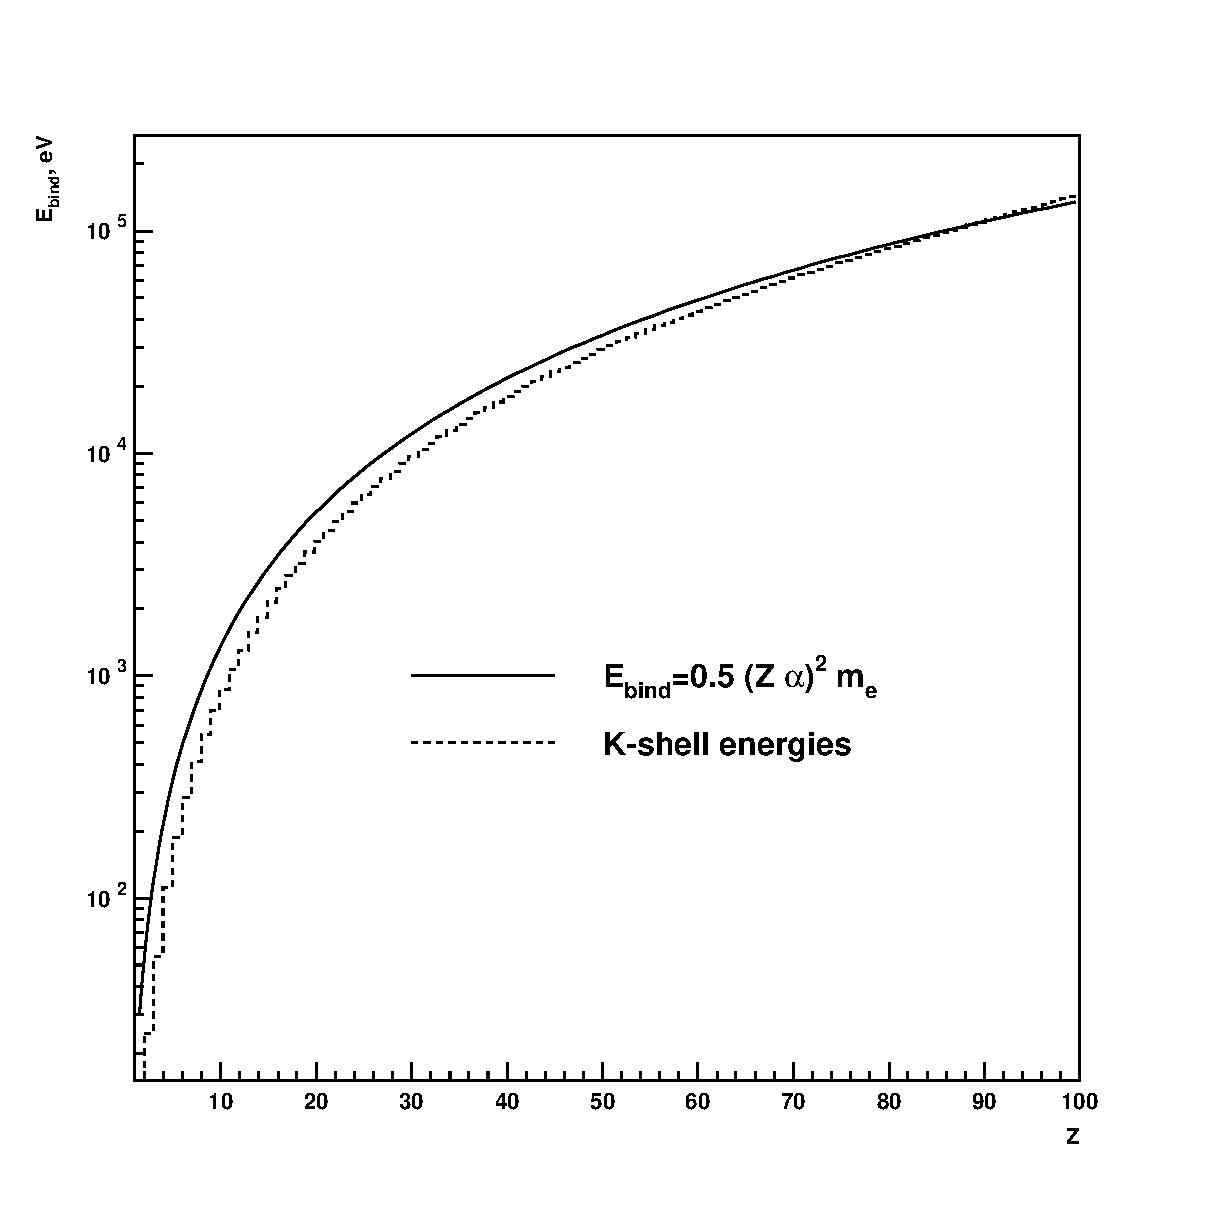
\epsfig{file=eps/phys351-1.eps,width=14cm}
   \caption{Comparison between the K-shell binding energies
            given by the expression in the text
            and the tabulated values. }
   \label{fg:phys351-1}
\end{figure}

Using the expression (\ref{eq:phys351-2}) with random numbers
$r_i \in ]0,1[, i=1,2$, the secondary photon energy is sampled by
the following steps:
\begin{enumerate}
\item sample $\epsilon$ from $f(\epsilon)$:
\begin{equation}
\epsilon =\epsilon_0 \exp  \left[ \ln \left(\frac{1- \epsilon_0}
{\epsilon_0}
          \right)  r_1  \right]
\end{equation}
\item
compute the rejection function $g(\epsilon)$ and
\begin{enumerate}
\item if $r_2 \leq g(\epsilon)$   accept $\epsilon$
\item if $r_1 > g(\epsilon)$  go back to 1.
\end{enumerate}
\end{enumerate}
After the successful sampling of $\epsilon$, the photon energy is computed as
 \begin{equation}
k = (E+m)\epsilon
\end{equation}
and then \Rind{GANNI} generates the polar angles of the photon with respect
to an axis defined by the momentum of the positron. The azimuthal angle
$\Phi$ is generated isotropically and $\Theta$ is computed from the
energy-momentum conservation. With this information, the momentum
vector of both photons can be calculated and transformed into the {\tt GEANT}
coordinate system.
 
The routine \Rind{GANNIR} treates the special case when a positron falls
below the cut-off energy ({\tt CUTELE} in 
common block \FCind{/GCCUTS/}) before annihilating.
In this case, it is assumed that the positron comes to rest before annihilating.
\Rind{GANNIR} generates two photons with energy $k=m$. The
angular distribution is isotropic.
\subsubsection{Annihilation into one photon}
The generated photon is assumed to be collinear with the positron.
Its energy will be
\begin{equation}
k = E + m_e - E_{bind}
\end{equation}
where $E_{bind}$ is the binding energy of the K-shell electron.
It can be estimated as follows
\begin{equation}
\label{eq:phys315-1}
E_{bind} = 0.5 (Z \, \alpha )^2  \, m_e
\end{equation}
where $\alpha$ is the fine stucture constant. The comparison
of this expression with the experimental data from
\cite{bib-XRAY} is shown in figure \ref{fg:phys351-1}.

\section{Restrictions}
\begin{enumerate}
\item
The annihilation processes producing three or more photons are
ignored, because these processes are negligible compared to the 
annihilation into two photons~\cite{bib-EGS3,bib-MES1};
\item
In calculating the process it is assumed that the atomic electron initially
is free and at rest. This is the usual assumption used in shower programs
\cite{bib-EGS3};
\end {enumerate}

%%%%%%%%%%%%%%%%%%%%%%%%%%%%%%%%%%%%%%%%%%%%%%%%%%%%%%%%%%%%%%%%%%%
%                                                                 %
%  GEANT manual in LaTeX form                                     %
%                                                                 %
%  Michel Goossens (for translation into LaTeX)                   %
%  Version 1.00                                                   %
%  Last Mod. Jan 24 1991  1300   MG + IB                          %
%                                                                 %
%%%%%%%%%%%%%%%%%%%%%%%%%%%%%%%%%%%%%%%%%%%%%%%%%%%%%%%%%%%%%%%%%%%
\Origin{I.Gavrilenko}
\Documentation{K.Lassila-Perini, I.Gavrilenko}
\Submitted{17.11.93} \Revised{16.12.93}
\Version{Geant 3.16}\Routid{PHYS360}
\Makehead{Synchrotron radiation}
\section{Subroutines}

\Shubr{GSYNC}{}
\Rind{GSYNC} is called for electron and positrons
when the flag {\tt ISYNC} is set $>$ 0. It 
computes the magnetic field and calls
\Rind{GSYNGE} for the generation of the synchrotron radiation
photons. It reads them in the {\tt GEANT} stack.
\Rind{GSYNC} is called from \Rind{GTELEC}.

\Shubr{GSYNGE}{(GAMMA,AMASS,FLDT,STEP,NTR,ETR,STR)}
\Rind{GSYNGE} generates the synchrotron radiation 
for an e$^-$ or e$^+$ with the Lorentz factor {\tt GAMMA}
in the magnetic field {\tt FLDT} and when the step
length is {\tt STEP}. The number of the secondary
photons is {\tt NTR}, their energy is in the array {\tt ETR} and
their position along the step is in {\tt STR}.
\Rind{GSYNGE} is called by \Rind{GSYNC}.


\section{Method}
A charged particle in a magnetic field emits radiation.
The number of photons emitted in a second is
\begin{equation}
\frac{d^2 \! N}{d\varepsilon \, dt} = \frac{15 \sqrt{3}}{8} \frac{P}{\varepsilon_c}
\end{equation}

where $\varepsilon_c$ is the critical photon energy
(the median of the energy spectrum) and $P$ the
total radiated power:

\begin{eqnarray}
\varepsilon_c & = & \frac{3}{2} \hbar c \frac{\gamma^3}{\rho} \\
P             & = & \frac{2}{3} \frac{ e^2 c}{\rho^2}\beta^4 \gamma^4
\end{eqnarray}
$\gamma$ is the e$^-$/e$^+$ Lorentz factor $E_{tot}/m_e$ and
$\beta = 1 - 1/\gamma^2$. $\rho$ is the
curvature caused by the magnetic field.
For more detailed derivation of these equations,
see \cite{bib-MAIE}.
The velocity of the particle being $\beta c$, the number of
photons per meter is
\begin{eqnarray}
\frac{d^2 \! N}{d\varepsilon \, dx}  & = & 
         \frac{d^2 \! N}{d\varepsilon \, dt} \, \frac{1}{\beta c} \nonumber \\
  & = & \frac{5 \sqrt{3}}{6} \frac{e^2}{\hbar c} 
        \beta^3 \gamma \frac{1}{\rho} \nonumber \\
  & = & \frac{5}{2 \sqrt{3}} \, \alpha \, \frac{\gamma}{\rho} 
        \; \approx  \; 0.01053 \, \frac{\gamma}{\rho}
\end{eqnarray}
The fine structure constant $\alpha = e^2/(\hbar c)$ and it is
assumed that $\beta^3 \approx 1$.

The curvature in a magnetic field $B$ which has a component
$B_{\perp}$ transversal to the particle velocity can
be computed \cite{bib-PDGB}
\begin{equation}
\rho = \frac{p} {0.3 B_{\perp}}
\end{equation} 
where $p$ is the momentum of the particle in GeV. $B$ is in tesla
and $\rho$ is in meters.

Knowing the step length, the energy of the electron
and the curvature of the particle track in the magnetic field,
the number of photons in a step $\delta x$ can be sampled from
a Poissonian distribution around the mean value
\begin{equation}
\overline{n_{\delta x}} = 0.01053 \, \frac{\gamma}{\rho} \delta x
\end{equation}

Now, the energies of $n_{\delta x}$ photons have to be determined.
The energy distribution in a step follows the distribution  \cite{bib-MAIE}
\begin{equation}
f(\varepsilon) \, = \, \frac{dN}{d\varepsilon} \, \propto \, 
        \int_{\varepsilon / \varepsilon_c}^{\infty} K_{5/3}(x) \, dx
\end{equation}
The energy can be sampled from this by inverse transform method:
\begin{eqnarray}
N \, & = & \, F(\varepsilon) = \, \int f(\varepsilon) \, d\varepsilon \\
\varepsilon \, & = & \, F^{-1}(N)
\end{eqnarray}
The double integral is not analytically solved, and the sampling
is done from tabulated values of numerically computes $F(\varepsilon)$. 


Two methods have been implemented. If the flag {\tt ISYNC}
is set to 1, the photons are emitted at the end of the step along the current
direction. If {\tt ISYNC} is set to 3, the photons are
emitted randomly along the tangent the real trajectory of the particle.
In the case when {\tt ISYNC = 3}, the magnetic field tracking routines are 
called for each photon, and therefore this option is
considrably slower than {\tt ISYNC = 1}.

\begin{figure}
\begin{picture}(300,100)(-60,0)

\put(40,80){{\tt ISYNC = 1}}
\put(0,0){\line(2,1){80}}
\put(80,40){\vector(1,0){20}}
\multiput(80,40)(16,0){4}{\vector(1,0){12}}
\put(45,15){{\tt STEP}}
\put(40,5){Current step}
\put(85,57){{\tt VECT}}
\put(85,47){New direction of e}
\put(90,25){Photons}

\put(240,80){{\tt ISYNC = 3}}
\put(200,0){\line(2,1){80}}
\put(280,40){\vector(1,0){20}}
\put(205,5){\circle*{.25}}
\put(210,9){\circle*{.25}}
\put(215,13){\circle*{.25}}
\put(220,16){\circle*{.25}}
\put(225,19){\circle*{.25}}
\put(230,22){\circle*{.25}}
\put(235,25){\circle*{.25}}
\put(240,27){\circle*{.25}}
\put(245,29){\circle*{.25}}
\put(250,31.5){\circle*{.25}}
\put(255,33.5){\circle*{.25}}
\put(260,35.){\circle*{.25}}
\put(265,36.5){\circle*{.25}}
\put(270,38){\circle*{.25}}
\put(275,39){\circle*{.25}}

\put(202,4){\vector(1,1){12}}
\put(218,16){\vector(4,3){12}}
\put(242,29){\vector(2,1){12}}
\put(263,37){\vector(3,1){12}}
\put(245,15){{\tt STEP}}
\put(240,5){Current step}
\put(285,57){{\tt VECT}}
\put(285,47){New direction of e}
\put(190,30){Photons}
\end{picture}
\caption{The point where the synchrotron radiation photon
         is generated. The figure on the left describes
         the situation when {\tt ISYNC = 1}, and the one
         on the right when {\tt ISYNC = 3}. The little
         arrows are the photons and {\tt STEP} is the
         step taken by the e$^-$ or e$^+$. {\tt VECT}
         is the new direction computed in {\tt GTELEC}
         before entering in {\tt GSYNC}.}
\end{figure}

%%%%%%%%%%%%%%%%%%%%%%%%%%%%%%%%%%%%%%%%%%%%%%%%%%%%%%%%%%%%%%%%%%%
%                                                                 %
%  GEANT manual in LaTeX form                                     %
%                                                                 %
%  Version 1.00                                                   %
%                                                                 %
%  Last Mod. 12 June 1993 18:20  MG                               %
%                                                                 %
%%%%%%%%%%%%%%%%%%%%%%%%%%%%%%%%%%%%%%%%%%%%%%%%%%%%%%%%%%%%%%%%%%%
\Origin{G.N.Patrick}
\Version{Geant 3.16}\Routid{PHYS400}
\Submitted {30.03.82} \Revised{16.12.93}
\Makehead{Simulation of particle decays in flight}
\section{Subroutines}
\Shubr{GDECAY}{}
 
\Rind{GDECAY} is the control routine for the simulation of particle
decays in flight. For a given parent particle it selects from a list a
two- or three-body decay mode using the known branching ratios and calls the
routines needed to generate the vertex and secondary tracks.
It used the following input and output:
\begin{DLtt}{MMMMMMM}
\item[input:]  via common blocks \FCind{/GCTRAK/} and \FCind{/GCKINE/}
\item[output:] via common block  \FCind{/GCKING/}
\end{DLtt}
\Rind{GDECAY} is called by the tracking routines.
It calls the subroutines 
\Rind{GDECA2} for two-body decay, \Rind{GDECA3} for three-body decay,
\Rind{GLOREN} for Lorentz transformation and \Rind{GDROT} for rotation.
For the documentation of \Rind{GLOREN} and \Rind{GDROT}, see {\tt [PHYS410]}.
\Shubr{GDECA2}{(XM0,XM1,XM2,PCM)}
\begin{DLtt}{MMMMMMMM}
\item[XM0] ({\tt REAL}) mass of the parent particle
\item[XM1] ({\tt REAL}) mass of the first decay product
\item[XM2] ({\tt REAL}) mass of the second decay product
\item[PCM(3,4)] ({\tt REAL}) array containing the four-vectors of
the decay products
\end{DLtt}
{\tt GDECA2} simulates the two-body decay with isotropic angular
distribution in the center-of-mass system. It is called from
{\tt GDECAY}.
\Shubr{GDECA3}{(XM0,XM1,XM2,XM3,PCM)}
\begin{DLtt}{MMMMMMMM}
\item[XM0] ({\tt REAL}) mass of the parent particle
\item[XM1] ({\tt REAL}) mass of the first decay product
\item[XM2] ({\tt REAL}) mass of the second decay product
\item[XM3] ({\tt REAL}) mass of the third decay product
\item[PCM(3,4)] ({\tt REAL}) array containing the four-vectors of
the decay products
\end{DLtt}
{\tt GDECA3} simulates the three-body decay 
with isotropic angular distribution in the center-of-mass system.
It is called from {\tt GDECAY}.

\section{Method}
\begin{itemize}
\item
Upon entry to \Rind{GDECAY} a binary search is made in a list of
parent particles. This list is stored in the {\tt JPART} structure
and currently contains the particles defined in \Rind{GPART}
{\tt [CONS300]}. If the current particle cannot be found in the list,
control is returned {\it without} any decay generation.
Up to six decay modes and their corresponding branching ratios are then
extracted from the {\tt JPART} data banks (see {\tt [CONS310]}).
\item
A decay channel is selected according to the branching ratios.
If the sum
of the branching ratios for a particle is not equal 100\%, it is
possible that {\it no} decay is selected.
\item
Depending on whether the two- or three-body decay is selected, either
\Rind{GDECA2} or \Rind{GDECA3} is called to generate the
four-momenta of the decay products with isotropic angular
distribution in the center-of-mass system.
\item
The momentum vectors of the decay products 
are transformed into the laboratory 
system and rotated back into the {\tt GEANT} coordinate frame.
The kinematics of the products is stored in the common \FCind{/GCKING/}.
\item
When a particle decays and no branching ratio is defined, then
\Rind{GDECAY}
calls the user routine \Rind{GUDCAY}.
\end{itemize}

%%%%%%%%%%%%%%%%%%%%%%%%%%%%%%%%%%%%%%%%%%%%%%%%%%%%%%%%%%%%%%%%%%%
%                                                                 %
%  GEANT manual in LaTeX form                              %
%                                                                 %
%  Michel Goossens (for translation into LaTeX)                   %
%  Version 1.00                                                   %
%  Last Mod. Jan 24 1991  1300   MG + IB                          %
%                                                                 %
%%%%%%%%%%%%%%%%%%%%%%%%%%%%%%%%%%%%%%%%%%%%%%%%%%%%%%%%%%%%%%%%%%%
\Origin{M. Hansroul}
\Version{Geant 3.16}\Routid{PHYS410}
\Submitted{01.09.76}    \Revised{16.12.93}
\Makehead{Rotations and Lorentz transformation}
\section{Subroutines}
\Shubr{GLOREN}{(BETA,PA,PB*)}
{\tt GLOREN} transforms the momentum and the energy from one 
Lorentz frame (A) to another (B). It uses the following input and output:
 
\begin{DLtt}{MMMMMMMM}
\item[BETA(4)] ({\tt REAL}) velocity components in light units
of frame B in frame A,
{\tt BETA(1$\ldots$3) $ = \vec{\beta}$, BETA(4)$=(1-\beta^2)^{-1/2} = 
\gamma$};
\item[PA(4)] ({\tt REAL}) momentum components in the frame (A);
\item[PB(4)] ({\tt REAL}) momentum components in the frame (B).
\end{DLtt}

{\tt GLOREN} is called from the routine {\tt GDECAY}.
The momentum $\vec{p}_A$ and energy $E_A$  in reference frame A are
transformed into the momentum $\vec{p}_B$ and energy $E_B$ in reference
frame B which translates with velocity $\vec{\beta}$ with respect
to A:
\begin{eqnarray*}
E_B        & = &\gamma (E_A - \vec{\beta}\cdot \vec{p}_A)\\
\vec{p}_B & = & \vec{p}_A +
\gamma \vec{\beta} \left(\frac{ \gamma \vec{\beta} \cdot \vec{p}_A}
{\gamma+1} - E_A \right)
\end{eqnarray*}

\Shubr{GDROT}{(P*,COSTH,SINTH,COSPH,SINPH)}
{\tt GDROT} rotates a vector from one reference system to another.

\begin{DLtt}{MMMMMMMM}
\item[P(3)] ({\tt REAL}) vector to rotate, overwritten on output;
\item[COSTH] ({\tt REAL}) cosine of the polar angle;
\item[SINTH] ({\tt REAL}) sine of the polar angle;
\item[COSPH] ({\tt REAL}) cosine of the azimuthal angle;
\item[SINPH] ({\tt REAL}) sine of the azimuthal angle;
\end{DLtt}

{\tt GDROT} is called from several routines to rotate a particle from
in the center-of-mass system to the {\tt GEANT} (laboratory) system.
The following rotation matrix is used:
\[ \left( \begin{array}{ccc}
\cos \theta \cos \phi & -\sin \phi   & \sin \theta \cos \phi \\
\cos \theta \sin \phi & \cos \phi    & \sin \theta \sin \phi \\
- \sin \theta         &  0           & \cos \theta     
\end{array}  \right )
=
\underbrace{
\left( \begin{array}{ccc}
\cos \phi & -\sin \phi & 0 \\
\sin \phi & \cos \phi  & 0 \\
0         &      0     & 1
\end{array}  \right )}_{\Dstm R_\phi}
\underbrace{
\left( \begin{array}{ccc}
\cos \theta  & 0 & \sin \theta \\
0            & 1 & 0           \\
-\sin \theta & 0 & \cos \theta
\end{array}  \right )}_{\Dstm R_\theta} \]
$R_\theta$ is a counterclockwise rotation around axis $y$ by an angle $\theta$, 
and $R_\phi$ is a counterclockwise rotation around axis $z'$ (rotated by an 
angle $\theta$ from the initial position) by an angle $\phi$.

\Shubr{GFANG}{(P,COSTH*,SINTH*,COSPH*,SINPH*,ROTATE*)}
\begin{DLtt}{MMMMMMMM}
\item[P(3)] ({\tt REAL}) input direction;
\item[COSTH] ({\tt REAL}) cosine of the polar angle;
\item[SINTH] ({\tt REAL}) sine of the polar angle;
\item[COSPH] ({\tt REAL}) cosine of the azimuthal angle;
\item[SINPH] ({\tt REAL}) sine of the azimuthal angle;
\item[ROTATE] ({\tt LOGICAL}) rotation flag, the rotation matrix is the unit
matrix if {\tt ROTATE=.FALSE.}, i.e. no rotation is needed;
\end{DLtt}

Find the sine and cosine of the polar and azimuthal angle of the direction
defined by the vector {\tt P}. If {\tt P} is along the $z$ axis, 
{\tt ROTATE=.FALSE.}.

\Shubr{GVROT}{(DCOSIN,PART*)}
\begin{DLtt}{MMMMMMMM}
\item[PART(3)] ({\tt REAL}) direction to be rotated, overwritten on output;
\item[DCOSIN(3)] ({\tt REAL}) direction of the new $z$ axis;
\end{DLtt}

Given the direction {\tt PART} in a system of reference $O$, it returns the
same direction in the system of reference where the $z$ axis of $O$ is
along {\tt DCOSIN}. This routine is very useful when the $\theta$
angle of a secondary particle is sampled in a reference frame where the
parent particle moves along the $z$ axis. Then the direction of the
secondary product in the {\tt MRS} is returned by \Rind{GVROT} if
{\tt DCOSIN} is the direction of the parent particle.

A call to \Rind{GVROT} is equivalent to the following code:
\begin{verbatim}
      DIMENSION PART(3), DCOSIN(3)
      LOGICAL ROTATE
      .
      .
      .
      CALL GFANG(DCOSIN,COSTH,SINTH,COSPH,SINPH,ROTATE)
      IF(ROTATE) CALL GDROT(PART,COSTH,SINTH,COSPH,SINPH)
\end{verbatim}

with the advantage that inside \Rind{GVROT} all calculations are performed
in double precision.

%%%%%%%%%%%%%%%%%%%%%%%%%%%%%%%%%%%%%%%%%%%%%%%%%%%%%%%%%%%%%%%%%%%
%                                                                 %
%  GEANT manual in LaTeX form                              %
%                                                                 %
%  Michel Goossens (for translation into LaTeX)                   %
%  Version 1.00                                                   %
%  Last Mod. Jan 24 1991  1300   MG + IB                          %
%                                                                 %
%%%%%%%%%%%%%%%%%%%%%%%%%%%%%%%%%%%%%%%%%%%%%%%%%%%%%%%%%%%%%%%%%%%
\Origin{G.N.Patrick, L.Urb\'{a}n, D.Ward}
\Version{Geant 3.16}\Routid{PHYS430}
\Submitted{12.03.82}  \Revised{16.12.93}
\Makehead{Ionisation processes for muons and protons}

\section{Subroutines}

\Shubr{GDRELA}{}

\Rind{GDRELA} initialises the ionisation energy-loss tables for different
materials and particles.
The energy binning is in the array
{\tt ELOW} (\FCind{/GCMULO/}) initialised in the routine \Rind{GPHYSI}.
The tables are filled with the quantity $dE/dx$ in GeV cm$^{-1}$,
for elements, mixtures and compounds. A
temporary table is also filled, containing 
additional points for integration, to obtain the range-energy
table (see {\tt [PHYS010]}).

\Rind{GDRELP} computes the ionisation energy loss for protons,
and the values are stored in the energy loss table.
This value is used for other charged hadrons with scaled energy bin.

\Rind{GDRELM} computes the ionisation energy loss for muons,
and sums it in the muon table
with the energy loss due to the other processes
(bremsstrahlung, pair production and nuclear interactions). 

The following pointers are used:

\begin{DLtt}{MMMMMMMMMMMMMMMMMM}
\item[JMA = LQ(JMATE-I)]    I$^{th}$ material bank;
\item[JEL1 = LQ(JMA-1)]     $dE/dx$ for \Pep/\Pem (see {\tt [PHYS330]});
\item[JEL2 = LQ(JMA-2)]     $dE/dx$ for $\mu^+/\mu^-$;
\item[JEL3 = LQ(JMA-3)]     $dE/dx$ for protons (used also 
for other charged particles).
\end{DLtt}

\Rind{GDRELA} is called during initialisation by \Rind{GPHYSI}.

\Shubr{GDRELP}{(A,Z,DENS,T,DEDX*)}

\Rind{GDRELP} computes the ionisation energy loss for 
protons. It is called by the routine \Rind{GDRELA}. See \Rind{GDRELX}
below for the meaning of the parameters.

\Shubr{GDRELM}{(A,Z,DENS,T,DEDX*)}

\Rind{GDRELM} computes the energy loss due to ionisation for 
muons. It is called by the routine \Rind{GDRELA}. See \Rind{GDRELX}
below for the meaning of the parameters.

\Shubr{GDRELX}{(A,Z,DENS,T,HMASS,DEDX*)}

\begin{DLtt}{MMMMMMMM}
\item[A] ({\tt REAL}) mass number of the material;
\item[Z] ({\tt REAL}) atomic number of the material;
\item[DENS] ({\tt REAL}) density of the material in g cm$^{-3}$; it is only used 
to calculate the density correction in case of high values of {\tt T};
\item[T] ({\tt REAL}) kinetic energy of the particle in GeV;
\item[HMASS] ({\tt REAL}) mass of the particle;
\item[DEDX] ({\tt REAL}) energy loss of the particle in GeV cm$^{2}$ g$^{-1}$.
\end{DLtt}

This routine calculates the ionisation energy loss for a muon or a
proton. It is called by \Rind{GDRELM} and \Rind{GDRELP}.


\Shubr{GDRSGA}{}

\Rind{CDRSGA} calculates the total cross-section for the production
of $\delta$-rays by electrons (M\"{o}ller scattering), positrons
(Bhabha scattering) and muons.
For hadrons, this value is calculated
at tracking time. The mean free path as a function of the energy
is stored for every medium. The following pointers are used: 

\begin{DLtt}{MMMMMMMMMMMMMMMMMM}
\item[JMA = LQ(JMATE-I)]  pointer to the I$^{th}$ material;
\item[JDRAY = LQ(JMA-11)]  $\delta$-ray cross-section for electrons;
\item[JDRAY+NEK1]  $\delta$-ray cross-section for positrons;
\item[JDRAY+2*NEK1]  $\delta$-ray cross-section for muons.
\end{DLtt}

The routine is called during initialisation by {\tt GPHYSI}.

\section{Method}

In {\tt GEANT}, $\delta$-rays are generated only above a threshold energy
$T_{cut}$ which corresponds to the variable {\tt DCUTE} for electrons and 
positrons, {\tt DCUTM} for all other charged particles. The total cross-section 
for the production of a $\delta$-ray electron of kinetic
energy $T > T_{cut}=${\tt DCUTE, DCUTM} by a particle of kinetic energy $E$
is:
\begin{equation}
\label{eq:phys430-3}
\sigma (E,T_{cut}) = \int_{T_{cut}}^{T_{max}} \frac{d \sigma (E,T)}{dT} dT
\end{equation}
where $T_{max}$ is the maximum energy transferable to the free electron:
\begin{equation}
T_{max} =\frac{2m(\gamma^2 -1)}
      {1+2\gamma\frac{m}{M}+
      \left(\frac{m}{M} \right)^2 }
\end{equation}

The energy lost in 
ionising collisions producing $\delta$-rays below ${T_{cut}}$
are included in the continuous energy loss. The mean value of the
energy lost due to these {\it soft} collisions is:
\begin{equation}
\label{eq:phys430-1}
E_{loss}(E,T_{cut}) = \int_{0}^{T_{cut}} 
T \frac{d \sigma (E,T)} {dT} dT
\end{equation}
where $m$ is the electron mass and $M$ is the mass of the incident particle.

In this chapter, the method of calculation of the continuous energy loss
and the total cross-section are
explained. The generation of $\delta$-rays is explained in 
chapter {\tt [PHYS331]}.

\subsection{Continuous energy loss}
The integration of (\ref{eq:phys430-1}) leads to the Bethe-Block
stopping power or to the restricted energy 
loss formula \cite{bib-PDGB}:
\begin{equation}
\label{eq:phys430-2}
\frac{1} {\rho} \left(\frac{dE}{dx} \right) =
\left \{
\begin{array}{LcL}
D \frac{Z Z_{inc}^{2}}{A \beta^{2}} \left [
\ln \left ( 
\frac{2 m_{e} \beta^{2} \gamma^{2} T_{max} }{I^{2}} 
\right ) - 2 \beta^{2} - 
\delta -
\frac{ 2 C_{e}}{Z} \right ] 
\hfill & \mbox{if} & T_{cut} \geq T_{max} \\ [0.5cm]
D \frac{Z Z_{inc}^{2}}{A \beta^{2}} \left [
\ln \left ( 
\frac{ 2 m_{e} \beta^{2} \gamma^{2} T_{c} }{I^{2}} 
\right ) - 
\beta^{2} \left ( 1 + \frac{T_{c}}{T_{max}} \right )
 - \delta
-\frac{2 C_{e}}{Z} \right ] \hfill & \mbox{if} & T_{cut} < T_{max}
\end{array} 
\right .
\end{equation}

where,
\[
\begin{array}{LL@{\hspace{2cm}}LL}
D & 2\pi N_A r_e^2 m c^2 = 0.000153537 \: \mbox{GeV cm$^2$ g$^{-1}$}
& Z & \mbox{atomic number of medium}  \\
A   & \mbox{mass number} & \rho & \mbox{density of medium} \\
T_c &  \min(T_{cut},T_{max}) & m_e & \mbox{electron mass}
\end{array}
\]

and $I$ is the average ionisation potential of the atom in question.
There exists a variety of phenomenological approximations for this.
In former versions of {\tt GEANT} the formula quoted by
\cite{bib-BRIC} was used ($I=16\:Z^{0.9}$ eV). At present the
values recommended by~\cite{bib-ANZI} are used. The ionisation
potential $I$ only enters into the logarithmic term of the energy
loss formula, but it has been verified that the new parameterisation
gives better accuracy especially in the case of high $Z$.
It should be noted that this is not the value of $I$ which
is stored in the material data structure by \Rind{GPROBI}, 
which is still calculated as $I=16\:Z^{0.9}$ eV.

{\bf Note:} the ionisation potential $I$ must not be changed blindly,
hoping that the most up-to-date values give the better results. The
value of $I$ is closely connected to the shell correction term (see
later). 

$\delta$ is a correction term which takes account of the reduction
in energy loss due to the so-called density effect. This becomes
important at high energy because media have a tendency to become
polarised as the incident particle velocity increases. As a consequence,
the atoms in a medium can no longer be considered as isolated. To correct
for this effect the formulation of Sternheimer~\cite{bib-STE1,bib-STE2} 
is used:
 
\begin{equation}
\delta = \left \{ \begin{array}{L@{\hspace{1cm}}lL} 
            0                   &    \mbox{if} & X  < X_0      \\
            4.606X + C + a(X_1-X)^m & \mbox{if} & X_0 \leq X < X_1 \\
            4.606X + C  & \mbox{if}  & X  \geq X_1
            \end{array} \right .
\end{equation}
 
where the medium-dependent constants are calculated as follows:
\[
\begin{array}{LcL@{\hspace{1.5cm}}LcL}
X & = & \log_{10}(\gamma \beta) = \ln(\gamma^{2} \beta^{2})/4.606 & 
\nu_{p} & = & \sqrt{ \frac{N_{el} e^2 }{\pi m} }
\mbox{\hspace{0.25cm}s$^{-1}$ plasma frequency} \\
N_{el} & = & \frac{\rho Z N_{Av}}{A} \mbox{\hspace{0.25cm}electrons cm$^{-3}$}
& C & = & -2 \ln \left ( \frac{I}{h\nu_{p}} \right ) - 1 \\
a & = & \frac{4.606(X_a - X_0)}{(X_1 - X_0)^m} & 4.606 \: X_{a} & = & -C
\end{array}
\]

For condensed media we have:
 
\[
\begin{array}{LL}
I < 100 \: \mbox{eV} & \left \{
\begin{array}{LcL}
X_{0} & = & \left \{
\begin{array}{LlL}
0.2 & \mbox{if} & -C \leq 3.681 \\
-0.326C-1.0 & \mbox{if} & -C > 3.681
\end{array} \right . \\
X_{1} & = & 2.0 \\
m & = & 3.0
\end{array} \right . \\ [1.0cm]
I \geq 100 \: \mbox{eV} & \left \{
\begin{array}{LcL}
X_{0} & = & \left \{
\begin{array}{LlL}
0.2 & \mbox{if} & -C \leq 5.215 \\
-0.326C-1.5 & \mbox{if} & -C > 5.215
\end{array} \right . \\
X_{1} & = & 3.0 \\
m & = & 3.0
\end{array} \right .
\end{array}
\]

and in the case of gaseous media $m=3$ and:

\[
\begin{array}{LLcr@{}c@{}l}
X_0 = 1.6 & X_1 = 4 & \mbox{for} &       & C & \leq 9.5 \\
X_0 = 1.7 & X_1 = 4 & \mbox{for} & 9.5 < & C & \leq 10 \\
X_0 = 1.8 & X_1 = 4 & \mbox{for} & 10  < & C & \leq 10.5 \\
X_0 = 1.9 & X_1 = 4 & \mbox{for} & 10.5 < & C & \leq 11 \\
X_0 = 2.  & X_1 = 4 & \mbox{for} & 11  < & C & \leq 12.25 \\
X_0 = 2.  & X_1 = 5 & \mbox{for} & 12.25 < & C & \leq 13.804 \\
X_0 = 0.326C-2.5 & X_1 = 5 & \mbox{for} & 13.804 < & C &  \\
\end{array}
\]

$C_e/Z$ is a so-called {\it shell correction term}
which accounts for the fact that, at
low energies for light elements and at all energies for heavy ones, the
probability of collision with the electrons of the inner atomic shells
(K, L, etc.) is negligible. The semi-empirical formula used in
{\tt GEANT}, applicable to all materials, is due to Barkas \cite{bib-BARK}:
\begin{eqnarray*}
 C_e(I,\eta) & = & (0.42237\eta^{-2}+0.0304\eta^{-4}-0.00038\eta^{-6})
10^{-6} I^2 \\
& +& (3.858\eta^{-2}-0.1668\eta^{-4}+0.00158\eta^{-6})10^{-9}I^3 \\
\eta & = &  \gamma \beta
\end{eqnarray*}
$C_e$ is a dimensionless constant, but as $I$ in the original
article was expressed in eV and in {\tt GEANT} it is expressed in GeV,
the exponent of ten in the $I^2$-term is $10^{-6+2 \times 9} = 10^{12}$, and
that of the $I^3$-term is $10^{-9+3 \times 9} = 10^{18}$.)
This formula breaks down at low energies, and it only applies for values 
of $\eta > 0.13$ (i.e. $T > 7.9$ MeV for a proton). For $\eta \leq
0.13$ the shell correction term is calculated as:

\[
\left . C_{e}(I,\eta) \rule{0mm}{5mm} \right |_{\eta \leq
0.13} = C_{e}(I,\eta=0.13)\frac{\ln \left ( \frac{T}{T_{2l}} \right )}
{\ln \left ( \frac{7.9 \: 10^{-3} \: \rm GeV}{T_{2l}} \right )}
\]
 
i.e. the correction is {\it switched off} logarithmically from $T=7.9$
MeV to $T=T_{2l}=2$ MeV.
\Rind{GDRELX} has been tested for protons against energy loss tables 
\cite{bib-SERR,bib-SER1}
for various materials in the energy range 50 MeV-25 GeV. 
Typical discrepancies are as follows:
 
\begin{flushleft}
\begin{tabular}{lll}
Beryllium: &   1.1\%  at 0.05 GeV      &  0.02\%  at  25 GeV\\
Hydrogen : &   1.5\%  at 0.05 GeV      &  12.1\%  at  25 GeV\\
Water   :  &   8.1\%  at 0.05 GeV      &  4.4\%  at  6  GeV\\
\end{tabular}
\end{flushleft}

The mean energy loss can be described by the Bethe-Bloch formula 
(\ref{eq:phys430-2}) only if the projectile velocity is larger than that
of orbital electrons. In the low-energy region where this is not 
verified, a different kind of parameterisation has been chosen \cite{bib-ANZI}:
\[
\frac{1}{\rho} \frac{dE}{dx} =  \left \{
\begin{array}{rLcL}
I: & C_{1} \tau^{\frac{1}{2}} & \mbox{for} & 0 \leq T \leq T_{1l} = 10 \:
\mbox{keV} \\
II: & \frac{S_{L} \times S_{H}}{S_{L} - S_{H}} & \mbox{for} & T_{1l}
< T \leq T_{2l} = 2 \: \mbox{MeV} \\
III: & \left \{ \mbox{Bethe-Bloch} \right \} \left ( 1+\frac{\nu}{T} \right )
& \mbox{for} & T_{2l} < T
\end{array} \right .
\]

where

\[
\begin{array}{LcL@{\hspace{1.5cm}}LcL}
S_{L} & = & C_{2} \tau^{0.45} & S_{H} & = & \frac{C_{3}}{\tau}
\ln \left [ 1+\frac{C_{4}}{\tau}+C_{5} \tau \right ] \\
\tau & = & \frac{T}{M_{p}} & M_{p} & = & \mbox{proton mass}
\end{array}
\]

\begin{table}
\begin{centering}
\begin{tabular}{l|c|c|c}
\multicolumn{4}{c}{$\displaystyle 
\frac{dE}{dx}^{calculated} - \frac{dE}{dx}^{measured}$}\\ [0.3cm]
\hline 
experiment & A~\cite{bib-REYN} & B~\cite{bib-GREE} & C~\cite{bib-SAKA} \\
\hline
projectile & p & p & p \\
T (MeV) & 0.03-0.6 & 0.4-1 & 55,65,73 \\ [0.2cm]
material 
& \parbox{3cm}{H$_2$, He, N$_2$, O$_2$, Ne, Ar, Xe}
& \parbox{3cm}{Cu, Ge, Sn, Pb}
& \parbox{3cm}{Al, Ti, Cu, Sn, Pb} \\
exp err (\%) & $\sim$ 3 & $\sim$ 2.5 & $\sim$ 0.7 \\
\hline\hline
tot N$^{\circ}$ of pts & 121 & 52 & 15 \\
\hline 
N$^{\circ}$ of pts \hfill & & & \\
\hfill with $|\Delta| < 1 \sigma$ & 94 & 50 & 8  \\
\hfill      $|\Delta| < 2 \sigma$ & 114 & 52 & 13  \\
\hfill      $|\Delta| < 3 \sigma$ & 119 & 52 & 14  \\
\hfill      $|\Delta| < 4 \sigma$ & 121 & 52 & 15  \\
\hline
\end{tabular}
\caption{Test of {\tt GDRELP} with low energy protons.}
\end{centering}
\label{tb:phys430-1}
\end{table}

The formula used in the region $T > T_{2l}$ ensures the continuity of the
energy loss function at $T = T_{2l}$ when the Bethe-Bloch formula and
the parameterisation meet. The parameter $\nu$ is chosen in such a
way that:

\[
\frac{1}{\rho} \left . \frac{dE}{dx}^{II} \right |_{T=T_{2l}} =
\frac{1}{\rho} \left . \frac{dE}{dx}^{III} \right |_{T=T_{2l}}
\]
 
The routine {\tt GDRELP} calculates the stopping power or restricted
energy loss only for $T > T_{2l}$; below this kinetic energy it gives
the stopping power (i.e. total energy loss) irrespectively of the 
value of $T_{cut}$. This approximation does not introduce a serious
source of error since, in the case of a proton, at $T=T_{2l}$ the 
maximum energy transferable to the atomic electron is $T_{max}
\approx 4$ keV, and the restricted loss should be calculated only if
$T_{cut} < T_{max}$.

{\tt GDRELP} has been tested against experimental data and energy loss
tables. Some of the test results are summarised in tables \ref{tb:phys430-1},
\ref{tb:phys430-2} and \ref{tb:phys430-3}.

\begin{table}
\begin{centering}
\begin{tabular}{rl|c|c}
\multicolumn{4}{c}{1 keV $ \leq T \leq $ 100 MeV,
31 pts per element~\cite{bib-ANZI}}\\
\hline
Z & element & \parbox{2.2cm}{mean (r.m.s.) deviation in \%} &
\parbox{2.2cm}{max (r.m.s.) deviation in \%} \\ [0.2cm]
\hline
1 & H$_2$ & 0.4 & 1.1 \\
6 & O & 0.5 & 1.6 \\
13 & Al & 0.6 & 2.1 \\
29 & Cu & 0.7 & 2.0 \\
82 & Pb & 0.7 & 2.3 \\
\hline
\end{tabular}
\caption{Test of {\tt GDRELP} against stopping power tables.
Stated accuracy of the tables is $\sim 5\%$ for $T > 0.5$ MeV and
$\sim 10\%$ for $T<0.5$ MeV}
\end{centering}
\label{tb:phys430-2}
\end{table}
The energy lost due to the soft $\delta$-rays is tabulated during
initialisation as a function of the medium and of the energy by routine
\Rind{GDRELA}

\begin{table}
\begin{centering}
\begin{tabular}{|l|r||l|r||l|r|}
\multicolumn{6}{c}{$\displaystyle
\Delta = \frac{\frac{dE}{dx}^{min}_{calc} - \frac{dE}{dx}^{min}_{table}}
{\frac{dE}{dx}^{min}_{table}} (\%)$} \\[0.5cm]
\multicolumn{6}{c}{Data from~\cite{bib-BAR1}} \\
\hline
material & $\Delta$ (\%) & material & $\Delta$ (\%) 
& material & $\Delta$ (\%)\\
\hline
H$_{2}$ & -0.4 & Na & -0.4 & Sn & 1.7 \\
D$_{2}$ & -0.3 & Al & -0.6 & Xe & 1.0 \\
He & 0.0 & Si & 0.5 & W & 1.1 \\
Li & 3.1 & Ar & 0.4 & Pt & 0.3 \\
Be & -0.2 & Ti & -1.4 & Pb & 1.5 \\
C & -0.1 & Fe & -0.4  & U & 1.4 \\
N$_{2}$ & -0.2 & Cu & -0.9 & & \\
O$_{2}$ & -1.2 & Ge & -0.8  & & \\
\hline
\end{tabular}
\caption{The minimum stopping power
calculated from the formula used is compared
with values from the tables.}
\end{centering}
\label{tb:phys430-3}
\end{table}

The tables are filled with the quantity $dE/dx$ in GeV cm$^{-1}$
(formula (\ref{eq:phys430-2})
above). For a molecule or a mixture the following formula
is used:
\begin{equation}
\frac{dE} {dx} = \rho \sum_{i} p_i
      \left( \frac{dE}{dX} \right)_i
\end{equation}
where $x$ is in cm, $X$ in g cm$^{-2}$ and $p_{i}$ is the proportion
by weight of the I$^{th}$ element.

The energy loss of all charged particles other than electrons,
positrons and muons is obtained from that of protons 
by calculating the kinetic energy of a proton with the same
$\beta$, and using this value to interpolate the tables:
\begin{equation}
 T_{proton} =\frac{M_{\rm p}}{M}T
\end{equation}

\subsection{Total cross-section}
The integration of formula (\ref{eq:phys430-3}) gives the total cross-section :
\begin{equation}
\label{eq:phys430-4}
\sigma (Z,E,T_{cut}) = \left \{
\begin{array}{LL}
2 \pi r^2_0 m  \frac{Z}{\beta^2}
   \frac{1-Y+\beta^2 Y\ln Y}{T_{cut}} & \mbox{for spin-0 particles} \\ [.5cm]
2 \pi r^2_0 m  \frac{Z}{\beta^2} \left (\frac{1-Y+\beta^2 Y\ln Y}{T_{cut}}
+ \frac{T_{max}-T_{cut}} {2E^2} \right) & 
\mbox{for spin-}\frac{1}{2}\mbox{~particles}
\end{array} \right .
\end{equation}

The mean free path is tabulated during initialisation 
as a function of the medium and of the energy by the routine
\Rind{GDRSGA}
{\it for leptons only}.
 
The cross-section (\ref{eq:phys430-4}) is strongly dependent on the mass of 
the incident
particle, and cannot be tabulated in a general way for any charged hadrons.
Therefore, for such particles, the cross-section is computed
at tracking time in the routine \Rind{GTHADR}.

%%%%%%%%%%%%%%%%%%%%%%%%%%%%%%%%%%%%%%%%%%%%%%%%%%%%%%%%%%%%%%%%%%%
%                                                                 %
%  GEANT manual in LaTeX form                              %
%                                                                 %
%  Michel Goossens (for translation into LaTeX)                   %
%  Version 1.00                                                   %
%  Last Mod. Jan 24 1991  1300   MG + IB                          %
%                                                                 %
%%%%%%%%%%%%%%%%%%%%%%%%%%%%%%%%%%%%%%%%%%%%%%%%%%%%%%%%%%%%%%%%%%%
\Origin{L.Urb\'{a}n}
\Version{Geant 3.16}\Routid{PHYS431}
\Submitted{12.03.82}  \Revised{16.12.93}
\Makehead{Ionisation processes for heavy ions}

\section{Subroutines}

For a description of the subroutines used to calculate the energy
loss tables for protons, see {\tt [PHYS430]}.

\Shubr{GTHION}{}

\Rind{GTHION} transports heavy ions ($A,Z > 1$, particle
type 8). For the moment the
only discrete processes activated are $\delta$-ray and \v{C}erenkov
photon generation.

\section{Method}

The mean energy loss of the heavy ions can be expressed as:
\begin{equation}
\Delta E = Q^{2} S_{p} \left ( \frac{T}{A} \right ) \rho t
\end{equation}
where
\begin{DLtt}{MMMMMMMMM}
\item[$Q$] charge of the ion;
\item[$\displaystyle S_{p} \left ( \frac{T}{A} \right )$]
energy loss by the a proton with kinetic energy $T_{p} = T/A$;
\item[$T,A$] kinetic energy and mass number of the ion;
\item[$\rho$] density of the medium;
\item[$t$] step length
\end{DLtt}

This formula is used to calculate the ionisation loss for all the charged
hadrons.


In the case of ions, the charge of the ion makes the problem more difficult.
Electron-exchange processes with the atoms change the
charge as the ion traverses the medium. The main features of this 
process can be summarised as follows:
\begin{itemize}
\item $Q$ loses the dependence on the initial ion charge after a
very short initial step, usually $\ll 1\mu$ for condensed media;
\item $Q$ does depend on the velocity of the ion;
\item even in the case of constant velocity, $Q$ fluctuates around
a mean value;
\item $Q$ features a small dependence on the medium, especially for
small values of $T$.
\end{itemize}
\begin{table}
\begin{centering}
\begin{tabular}{|c|c|c|}
\hline
T/A & He ions & Pb ions \\
MeV & error (\%) & error (\%) \\
\hline
10 & 3 &  1 \\
5 & 4 & 3 \\
3 & 10 & 4 \\
\hline
\end{tabular}
\caption{Comparison of the measured and calculated $\Delta$E for 10 MeV/A
ions in Pb}
\end{centering}
\label{tb:phys431-1}
\end{table}

If we want to calculate the energy loss of the ion, we need a good
parametrisation for the quantity $Q=Q_{eff}$. We give here a 
relatively simple parametrisation~\cite{bib-ANZI,bib-ANZ1}:
\begin{eqnarray}
\label{eq:phys431-2}
Q_{eff} & = & Z_{I} \left [ 1- \left ( 1.034 - 0.1777 e^{-0.08114\;Z_{I}}
\right ) e^{-v} \right ] \\
v & = & 121.4139 \frac{\beta}{Z_{I}^{2/3}} + 0.0378
\sin \left ( 190.7165 \frac{\beta}{Z_{I}^{2/3}} \right ) \nonumber
\end{eqnarray}
where $\beta$ is the velocity and $Z_{I}$ the atomic number of the ion
(i.e. the charge of the bare nucleus).

\begin{table}
\begin{centering}
\begin{tabular}{|r|rr|rr|r|r|rr|rr|r|r|}
\hline
\multicolumn{1}{|c|}{T (MeV)} & \multicolumn{6}{c|}{417 $\mu$g cm$^{-2}$}
& \multicolumn{6}{c|}{110 $\mu$g cm$^{-2}$} \\[0.1cm]
& \multicolumn{4}{c|}{MC (keV)} & \multicolumn{2}{c|}{data (keV)} &
\multicolumn{4}{c|}{MC (keV)} & \multicolumn{2}{c|}{data (keV)} \\
& $\Delta$E & dif & FWHM & dif & $\Delta$E & FWHM & 
$\Delta$E & dif & FWHM & dif & $\Delta$E & FWHM \\
\hline
4.88  & &  & & & & & 785 & 8 & 59 & -23 & 725 & 77 \\
9.85 & 3600 & 14 & 138 & -33 & 3150 & 206 & 816 & 8 & 67 &  -26 & 756 & 91 \\
19.79 & 3090 & 3 & 142 & -35 & 2990 & 218 & 719 & 3 & 70 & -32 & 699 & 103 \\
29.27 & 2660 & 1 & 141 & -31 & 2630 & 204 & & & & & & \\
29.75 & & & & & & & 620 & 4 & 69 & -26 & 598 & 93 \\
39.70 & 2320 & 1 & 138 & -28 & 2300 & 191 & 550 & 4 & 68 & -24 & 528 & 90 \\
\hline
\end{tabular}
\caption{Comparison of the measured and calculated $\Delta$E and FWHM
for O ions in Al; errors are in percent.}
\end{centering}
\label{tb:phys431-2}
\end{table}

It can be seen that (\ref{eq:phys431-2}) neglects the (small) medium
dependence of $Q_{eff}$. For very high energies ($\beta \rightarrow 1$)
$Q_{eff} \rightarrow Z_{I}$. For very low energies ($T/A \sim$ few keV)
the formula breaks down. $Q_{eff}$ can even become negative for $T/A <
20$ keV and $Z_{I} > 20$. However this is not a serious source of
error when calculating $\Delta E$, since in this case the range of
the ion is very small, and it can almost be said that it stops
{\it immediately}.

The calculation of the energy loss straggling (fluctuations) differs
from that of {\it normal} charged hadrons. For the charged hadrons
the fluctuations come from the statistical nature of the 
projectile-atom interactions; for the ions there is another process which
broadens the energy loss distribution: the fluctuation of the charge.
For heavier ions this process dominates the energy loss straggling
for $T/A \leq 10$ MeV.

\begin{figure}[hbt]
     \centering
     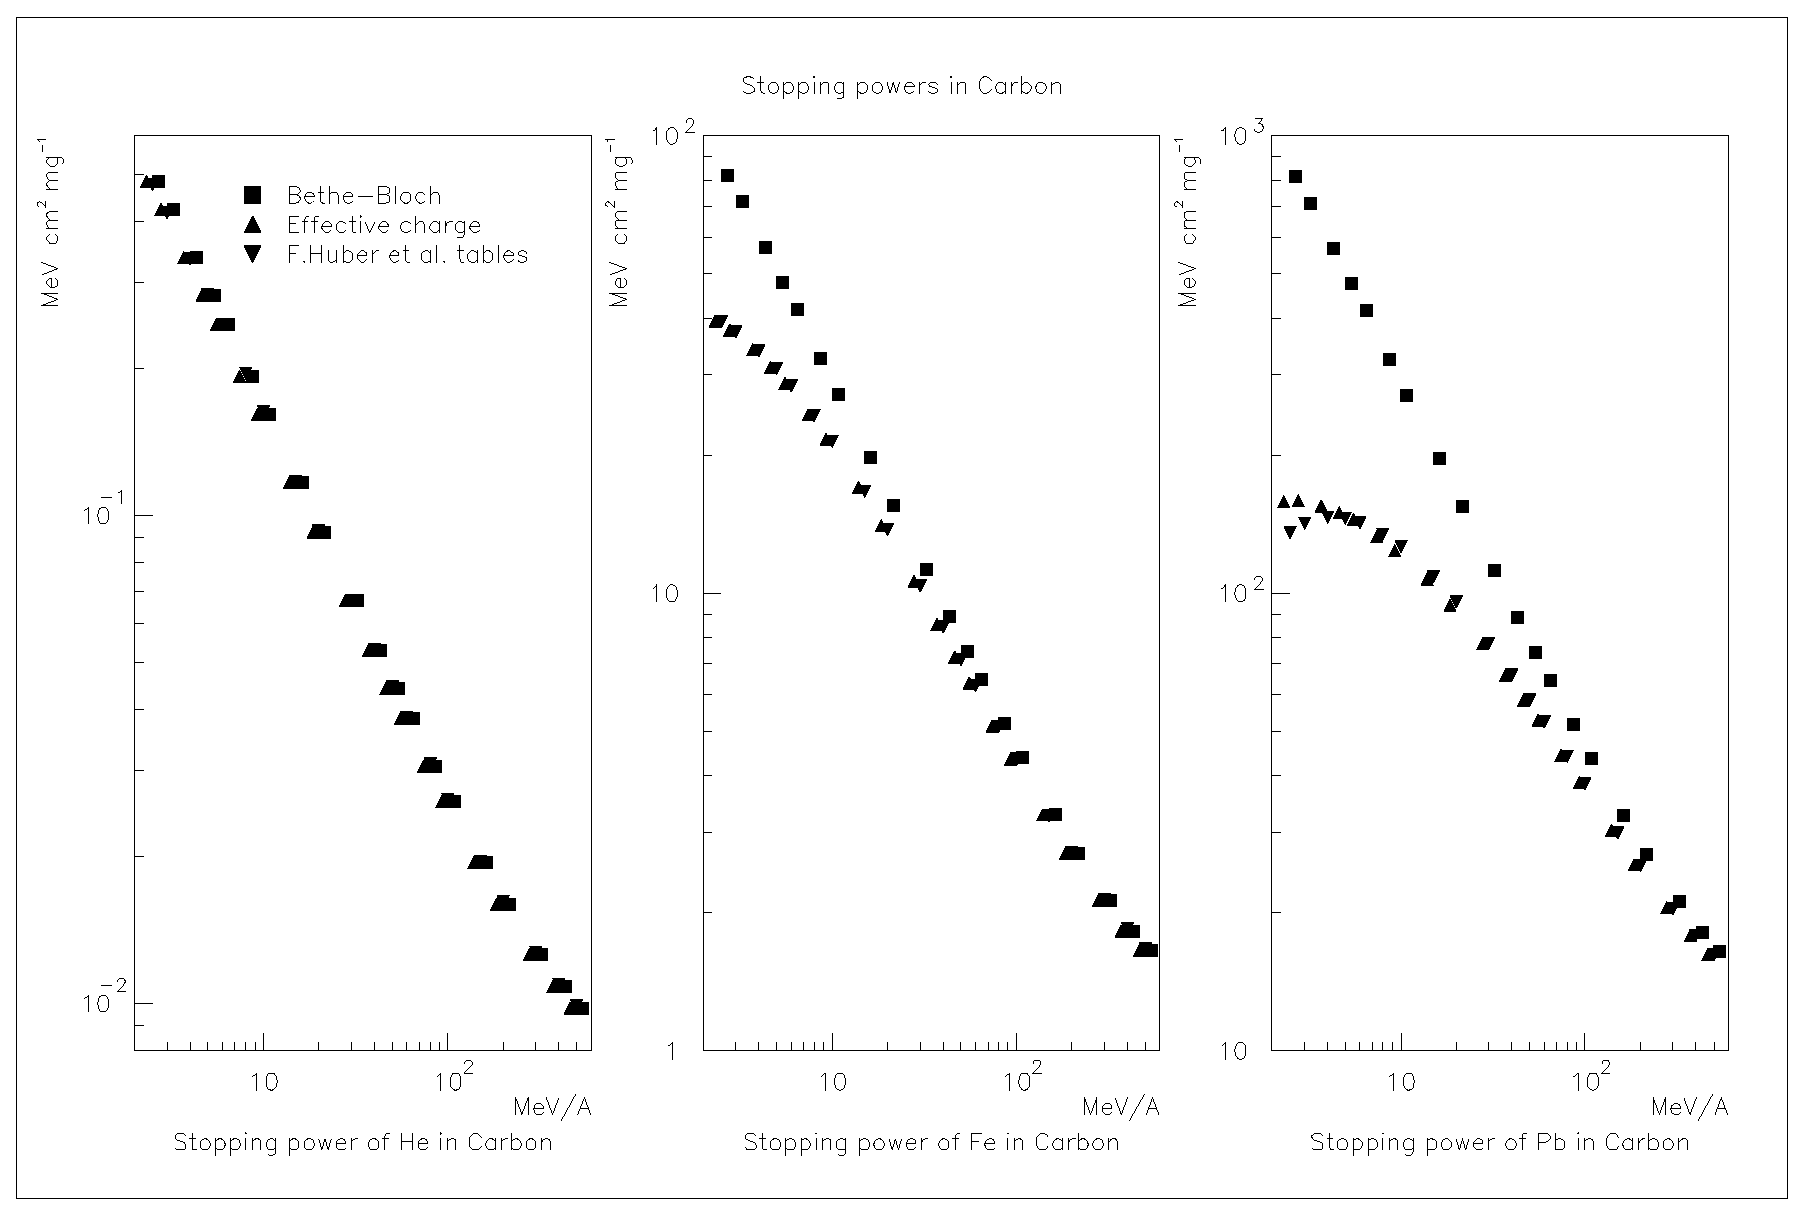
\epsfig{file=eps/phys431-1.eps,width=14cm}
     \caption{Stopping powers in Carbon}
     \label{fg:phys431-1}
\end{figure}

The heavy ions are in the {\it Gaussian regime} (see {\tt [PHYS332]})
of the collisional fluctuations even in the case of very thin absorbers.
If $T/A$ is not too high, the $\sigma^{2}$ of the distribution:
\begin{equation}
\label{eq:phys431-3}
\sigma^{2}_{coll} = D \frac{Q_{eff}^{2} Z}{A} \rho \; t \; m
\left [ 1 + \frac{T_{A}}{M_{u}} + \frac{1}{2} \left ( \frac{T_{A}}{M_{u}}
\right ) ^{2} \right ]
\end{equation}
where
\begin{DLtt}{MMMMMMMM}
\item[$D$] $\displaystyle 0.307 \frac{\mbox{MeV cm$^{2}$}}{\mbox{g}}$;
\item[$T_{A}$] $\displaystyle \frac{T}{A}$;
\item[$M_{u}$] atomic mass unit;
\item[$Z$] atomic number of the medium;
\item[$A$] mass number of the medium.
\end{DLtt}

\begin{table}
\begin{centering}
\begin{tabular}{|r|rr|r|rr|r|rr|r|}
\hline
& \multicolumn{9}{c|}{Pb ions in gas (energies in MeV)} \\
& \multicolumn{3}{c|}{N$_{2}$} & 
\multicolumn{3}{c|}{Ar} & 
\multicolumn{3}{c|}{Xe} \\
& \multicolumn{2}{c}{MonteCarlo} & \multicolumn{1}{c|}{data} &
\multicolumn{2}{c}{MonteCarlo} & \multicolumn{1}{c|}{data} &
\multicolumn{2}{c}{MonteCarlo} & \multicolumn{1}{c|}{data} \\
t (cm) & 
$\Delta$E & FWHM & FWHM & $\Delta$E & FWHM & FWHM & $\Delta$E & FWHM & FWHM \\
\hline
0.2 & 25.9 & 1.15 & 1.1 & 25.4 & 1.30 & 1.4 & 51.1 & 2.26 & 2.5 \\
0.4 & 53.6 & 1.62 & 1.5 & 52.4 & 1.84 & 1.9 & 107.0 & 3.22 & 3.3 \\
0.8 & 112.0 & 2.25 & 2.0 & 111.0 & 2.59 & 2.6 & 236.0 & 4.51 &  \\
1.2 & 162.0 & 2.37 & 2.0 & 168.0 & 2.95 & 2.8 & & & \\
\hline
\end{tabular}
\caption{Comparison of the measured and calculated and FWHM
for 1.4 MeV/A Pb ions in gas.}
\end{centering}
\label{tb:phys431-3}
\end{table}

Analysing the experimental straggling data it is possible to find that
the electron-exchange charge fluctuations can be described by a Gaussian
with width:
\begin{equation}
\label{eq:phys431-4}
\sigma^{2}_{ch} = D \frac{Q_{eff}^{2} Z}{A} \rho \; t \; m \frac{C}{2}
\left ( 1 - \frac{Q_{eff}}{Z_{I}} \right )
\end{equation}
where the parameter $C \sim 2.5$ has been derived
from the experimental straggling data.

If $Q_{eff} \rightarrow Z_{I}$, which is the case for high energy
heavy ions and for few MeV/A He ions, then $\sigma^{2}_{ch} \rightarrow 0$.


Comparing equations (\ref{eq:phys431-3}) and (\ref{eq:phys431-4}) it can be 
seen that for heavy ions and for $T/A \ll M_{u}$ $\sigma^{2}_{ch}
> \sigma^{2}_{coll}$. The total energy loss fluctuation can be
described by a Gaussian distribution with:
\begin{equation}
\sigma^{2} = \sigma^{2}_{ch} + \sigma^{2}_{coll}
\end{equation}

The mean energy loss and energy loss fluctuation calculation is performed
in the routine \Rind{GTHION}, making use of the proton energy loss tables.

{\bf Note:} The Gaussian fluctuation gives too broad a distribution for
high energy in the case of thin absorbers. A correction has been introduced
in \Rind{GTHION} which cures this discrepancy. In the absence of high
energy straggling data for ions, the correction has been tuned using 
high energy $\pi$ energy loss data, where the $\pi$ has been tracked
by \Rind{GTHION}.

\section{Comparison with data}

\subsection{Mean energy loss and range}

A test has been made against the distributions reported in~\cite{bib-HEIN}
for He ions at 1 and 10 MeV/A and for O and Pb ions at 1, 10 and
100 MeV/A in carbon and the results were found
to be correct within $5\%$ both for the energy loss and the range.

\begin{figure}[hbt]
     \centering
     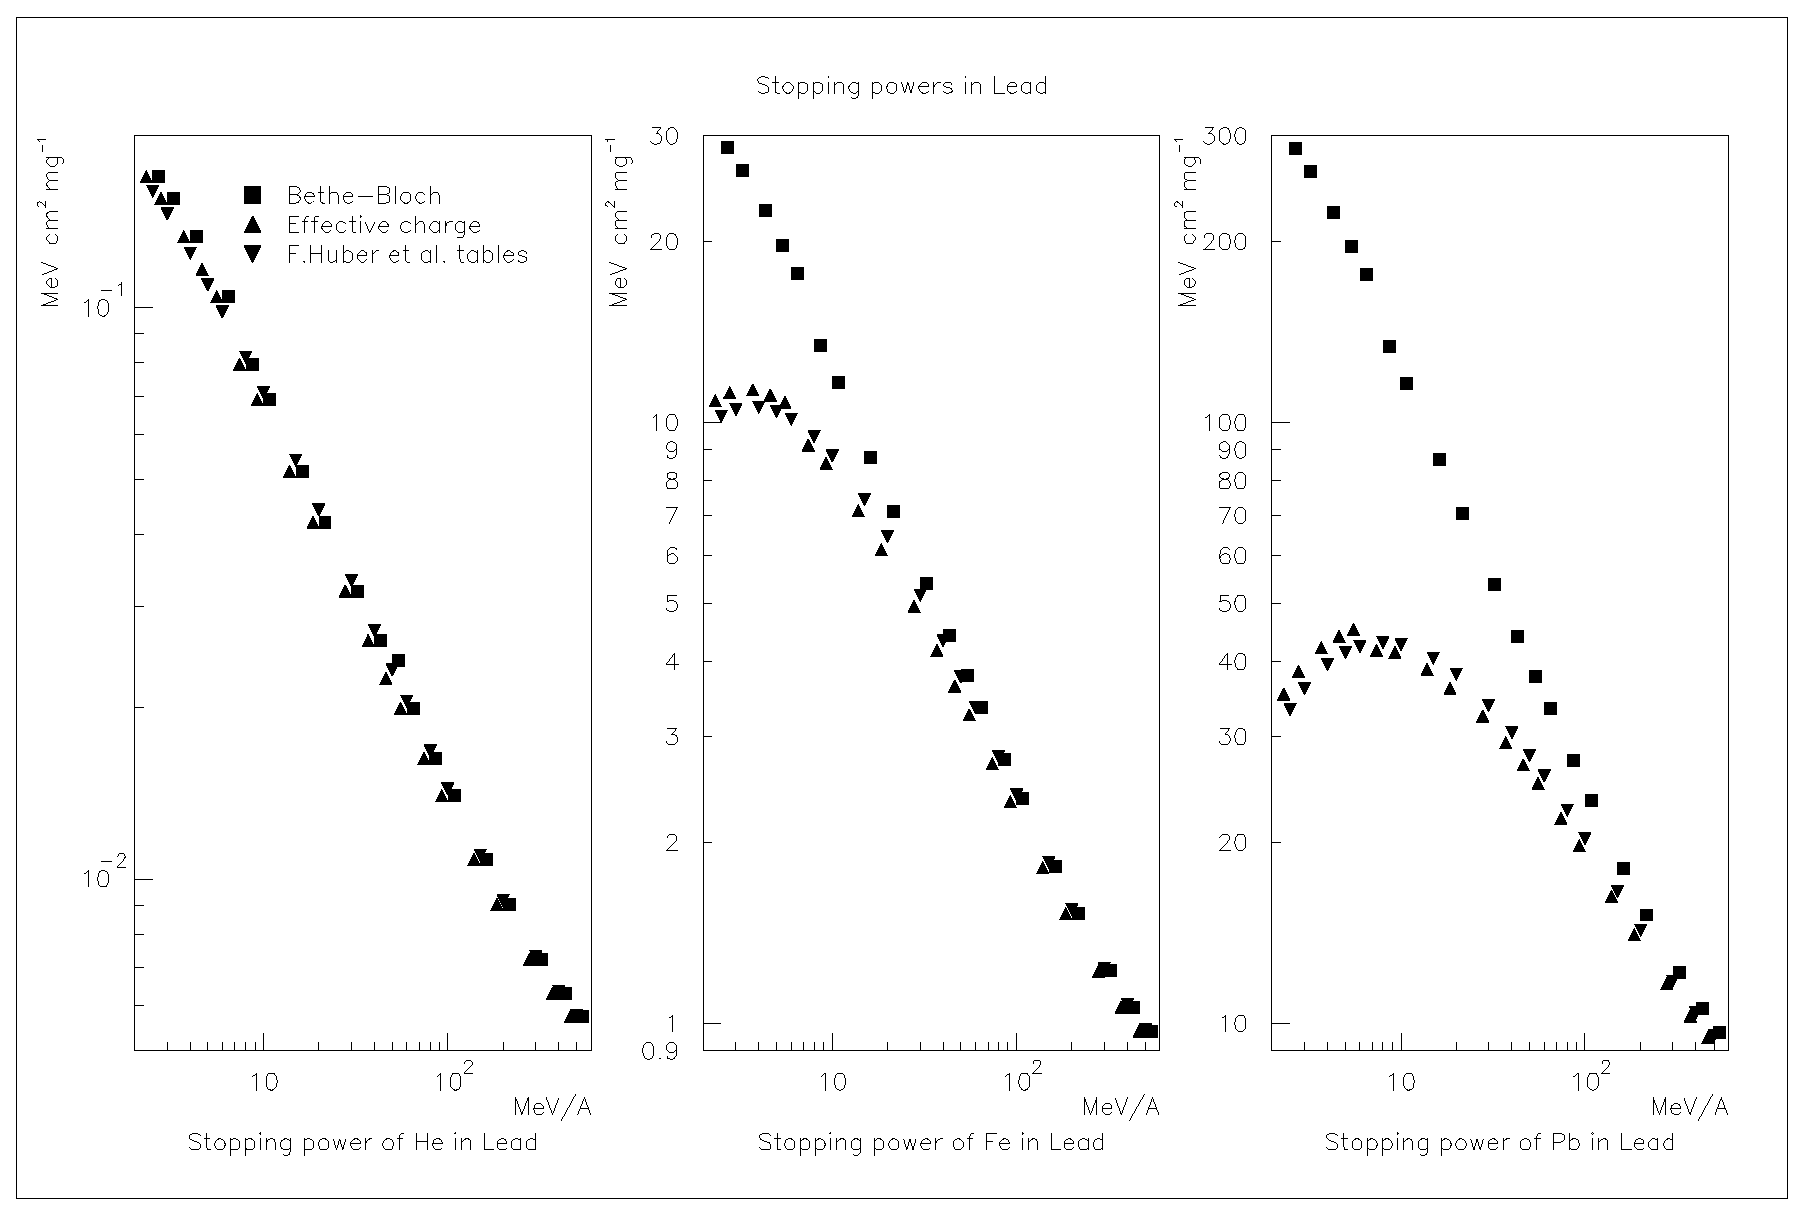
\epsfig{file=eps/phys431-2.eps,width=14cm}
     \caption{Stopping powers in Lead}
     \label{fg:phys431-2}
\end{figure}

Another comparison has been made with the tables of~\cite{bib-HUBE} 
for 10 MeV/A ions in lead, with
the results shown in table~\ref{tb:phys431-1}.
Another comparison with the same tables is shown in Figs.~\ref{fg:phys431-1}
and \ref{fg:phys431-2}.

A comparison with the tables in~\cite{bib-ANZI,bib-ANZ1} for T/A $<$ 1 MeV/A
gives  an error on $(dE/dx) \leq 10-20\%$.

\begin{table}
\begin{centering}
\begin{tabular}{|r|rr|r|}
\hline
\multicolumn{4}{|c|}{He ions in Ar (energies in keV)} \\
& \multicolumn{2}{c}{MonteCarlo} & \multicolumn{1}{c|}{data} \\
t (cm) & 
$\Delta$E & FWHM & FWHM \\
\hline
0.5 & 444 & 38 & $\sim$40 \\
1.0 & 913 & 53 & $\sim$60 \\
2.0 & 1940 & 78 & $\sim$80 \\
\hline
\end{tabular}
\caption{Comparison of the measured and calculated and FWHM
for 1.4 MeV/A He ions in gas.}
\end{centering}
\label{tb:phys431-4}
\end{table}

\subsection{Comparison of FWHM}

A comparison has been made with 
low energy data ($0.3 \leq T/A \leq 2.5$ MeV/A) in very
thin absorbers (1,7 $\mu$m, 0.4 $\mu$m). Data are taken from
the tables in~\cite{bib-TSCH} for
energy loss of O ions in Al, and the
results are reported in table~\ref{tb:phys431-2}. The quoted experimental 
error for these data is $1\%$ statistical + $5\%$ systematic for 
417 $\mu$g cm$^{-2}$ data and $2\%$ statistical + $10\%$ systematic for
110 $\mu$g cm$^{-2}$ data. 

Plots of energy deposition distributions of 1.4 MeV/A lead and helium
ions in gases can be found in~\cite{bib-GEIS}. 
From these we have measured the FWHM and compared them with the ones given
by the MonteCarlo. The results can be seen in table~\ref{tb:phys431-3}
and ~\ref{tb:phys431-4}. It
should be noted that the absorber thickness of, for example, Ar compares
with that of the preceding case (0.2 cm Ar = 356 $\mu$g cm$^{-2}$ and
1.2 cm Ar = 2136 $\mu$g cm$^{-2}$).


Similar comparison has been made for C ions of energies 17.1 and 39.4 MeV in 
isobuthane~\cite{bib-SCHM} and the agreement between data and {\tt GEANT}
for FWHM is within 30\%.

%%%%%%%%%%%%%%%%%%%%%%%%%%%%%%%%%%%%%%%%%%%%%%%%%%%%%%%%%%%%%%%%%%%
%                                                                 %
%  GEANT manual in LaTeX form                              %
%                                                                 %
%  Michel Goossens (for translation into LaTeX)                   %
%  Version 1.00                                                   %
%  Last Mod. Jan 24 1991  1300   MG + IB                          %
%                                                                 %
%%%%%%%%%%%%%%%%%%%%%%%%%%%%%%%%%%%%%%%%%%%%%%%%%%%%%%%%%%%%%%%%%%%
\Origin{L.Urb\'{a}n}
\Version{Geant 3.16}\Routid{PHYS440}
\Submitted{26.10.84}  \Revised{16.12.93}
\Makehead{Total cross-section and energy loss for bremsstrahlung by
Muons}
\section{Subroutines}
\Shubr{GBRELA}{}
{\tt GBRELA} fills the tables for continuous energy loss of electrons,
positrons and muons due to bremsstrahlung during initialisation time.
The energy binning is determined by
the array {\tt ELOW} (common \FCind{/CGMULO/}) in the
routine \Rind{GPHYSI}. In the tables, the $dE/dx$ due to bremsstrahlung
is summed with that due to the ionisation. For energy loss
of muons, \Rind{GBRELA} calls the function \Rind{GDRELM}.
The following pointers are used:
\begin{DLtt}{MMMMMMMMMMMMMMMMMM}
\item[JMA = LQ(JMATE-I)] pointer to the I$^{th}$ material;
\item[JEL1 = LQ(JMA-1)]  pointer to dE/dx for electrons;
\item[JEL1+NEK1]           pointer to dE/dx for positrons;
\item[JEL2 = LQ(JMA-2)]  pointer to dE/dx for electrons.
\end{DLtt}
\Rind{GBRELA} is called by \Rind{GPHYSI}.
\Sfunc{GBRELM}{VALUE = GBRELM(Z,T,BCUT)}
\begin{DLtt}{MMMMMMMM}
\item[Z] ({\tt REAL}) atomic number of the material;
\item[T] ({\tt REAL}) kinetic energy of the muon;
\item[BCUT] ({\tt REAL}) {\it soft} bremsstrahlung cut.
\end{DLtt}
\Rind{GBRELM} calculates the muon energy loss due to bremsstrahlung
of photons with energy below {\tt BCUT}, (variable {\tt BCUTM} in the
common \FCind{/GCCUTS/}).
Above this value, the bremsstrahlung process is simulated
explicitly (see {\tt [PHYS441]}) and the energy lost by the muons is
not included in the tables. 
In the tables, the $dE/dx$ due to bremsstrahlung is summed with
the energy lost coming from ionisation, pair production and nuclear interaction.
\Rind{GBRELM} is called by \Rind{GBRELA}.
\Shubr{GBRSGA}{}
{\tt  GBRSGA} calculates the total cross-section for bremsstrahlung.
It tabulates the mean free path
in cm as a function of the medium and the energy. The energy
binning is determined by the array {\tt ELOW} (common \FCind{/CGMULO/}).
The following pointers are used:
\begin{DLtt}{MMMMMMMMMMMMMMMMMM}
\item[JMA = LQ(JMATE-I)]pointer to the I$^{th}$ material;
\item[JBREM = LQ(JMA-9)]pointer to bremsstrahlung cross-sections;
\item[JBREM            ]pointer for \Pem;
\item[JBREM+NEK1       ]pointer for \Pep;
\item[JBREM+2*NEK1     ]pointer for $\mu^+/\mu^-$.
\end{DLtt}
\Rind{GBRSGA} is called during initialisation by \Rind{GPHYSI}.
\Sfunc{GBRSGM}{VALUE = GBRSGM(Z,T,BCUT)}
\begin{DLtt}{MMMMMMMM}
\item[Z] ({\tt REAL}) atomic number of the materian;
\item[T] ({\tt REAL}) kinetic energy of the muon;
\item[BCUT] ({\tt REAL}) {\it soft} bremsstrahlung cut.
\end{DLtt}
\Rind{GBRSGM} calculates the total bremsstrahlung cross-section for
muons when the emitted photon has an energy greater than {\tt BCUT}, 
(variable {\tt BCUTM} in the common \FCind{/GCCUTS/}). It is called
by \Rind{GBRSGA}.
\section{Method}
 
The mean value of the energy lost by the muon due to bremsstrahlung of
photons of energy $<k_{c}$ = {\tt BCUTM} is:
\begin{equation}
\label{eq:phys440-1}
E_{loss}^{brem}(Z,T,k_c ) = \int_{0}^{k_c} k
        \frac{d \sigma (Z,T,k)}{dk}dk
\end{equation}
and the total cross-section for the emission of a photon of energy
$ > k_c $ is
\begin {equation}
\label{eq:phys440-2}
 \sigma (Z,T,k_c ) = \int_{k_c}^{T}
        \frac{d \sigma (Z,T,k)} {dk} dk
\end{equation}
Accurate cross-section formula for the high energy ($T \geq 1$ GeV)
muon bremsstrahlung can be found in \cite{bib-LOHM}.

\subsection{Parameterisation of energy loss and total cross-section}
The cross-sections from \cite{bib-LOHM} have been used to calculate 
{\it data} points for (\ref{eq:phys440-1}) and (\ref{eq:phys440-2}).
These have been parameterised as:
\[ \begin{array}{LcLl}
 \sigma (Z,T,k_c)& =& Z[Z+ \xi_{\sigma}(1+ \gamma \ln Z)]
       \left[\ln \frac{k_{max}}{k_c}\right]^{\alpha}
       F_{\sigma}(Z,X,Y) & \mbox{ in barn} \\
  E_{loss}^{brem} (Z,T,k_c)   & = & Z[Z+\xi_l(1+\delta\ln Z)]
   \left[\ln\frac {k_c} {E} \right]^{\beta}
    F_l(Z,X,Y) & \mbox{ in GeV barn}
\end{array} \]
\[ \begin{array}{LcL@{\hspace{2cm}}LcL}
k_{max} & = & E-0.75 \sqrt {e}m_{\mu}Z^{1/3} & X & = & \ln \frac{E}{m_{\mu}} \\
Y & = & \ln \frac{k_c}{m_{\mu}} & E & = & T+m_{\mu}
\end{array} \]
where  $k_{max}$ is the maximum
possible value of the photon energy.
The functions $F_i(Z,X,Y)$ ($i=\sigma ,l$) are polynomials:
\begin{eqnarray}
\label{eq:phys440-3}
F_i(Z,X,Y) & = & (C_1+C_2X+\cdots +C_6X^5)+(C_7+C_8X+\cdots+C_{12}X^5)Y
\nonumber \\
        & + & \cdots + (C_{31}+C_{32}X+\cdots+C_{36}X^5)Y^5
\nonumber \\
           & + & Z[(C_{37}+C_{38}X+\cdots+C_{40}X^3)+(C_{41}+C_{42}X+
                   \cdots+C_{44}X^3)Y \nonumber \\
           & + & \cdots + (C_{48}+C_{49}X+\cdots+C_{52}X^3)Y^3)]
\end{eqnarray}
A least-squares fit has been performed on more than 2000 points for
$Z = 1, 6, 13, 26, 50, 82, 92$ and 1 GeV $\leq T \leq $ 10 TeV and
10 keV $\leq k_c \leq T $. The resulting values of 
$\xi_{\sigma,l}$, $\gamma$, $\alpha$ ,$C_i$, $\xi_l$, $\delta$ and $\beta$
can be found in the {\tt DATA} statements within the functions
\Rind{GBRSGM} and \Rind{GBRELM} which
compute formulae (\ref{eq:phys440-1}) and (\ref{eq:phys440-2}) respectively.
 
The accuracy of the fit can be estimated as:\\
 
\[ \begin{array}{LcL}
\frac{\Delta \sigma}{\sigma} & = & \left \{
\begin{array}{p{2cm}lL}
$\displaystyle 10-12\%$ & \mbox{if} & T \leq 5 \: \mbox{GeV} \\
$\displaystyle \leq 4\%$ & \mbox{if} & T > 5 \: \mbox{GeV}
\end{array} \right . \\ [0.5cm]
\frac{\Delta E_{loss}^{brem}}{E_{loss}^{brem}} & = & \left \{
\begin{array}{p{2cm}lL}
$\displaystyle 10\%$ & \mbox{if} & T \leq 5 \: \mbox{GeV} \\
$\displaystyle \leq 3\%$ & \mbox{if} & T > 5 \: \mbox{GeV}
\end{array} \right .
\end{array} \]
 
The contribution of the bremsstrahlung to the total energy loss of
the muons is less than 1\% for $ T \leq$ 5 GeV.
 
When $k_{c} \geq k_{max}$, a parameterisation different from 
(\ref{eq:phys440-3}) can be used for the total muon energy loss due to 
bremsstrahlung:
\begin{eqnarray} 
\label{eq:phys440-4}
E_{loss}^{brem} (Z,T) & = & E_{loss}^{brem}(Z,T,k=k_{max}) 
\nonumber\\
& = & Z(Z+1) k_{max}[d_1+(d_2X+d_3Y) + (d_4X^2+d_5 XY+d_6 Y^2) \nonumber \\
& + & \cdots+(d_{22}X^6+d_{23}X^5 Y+\cdots+d_{28}Y^6)]
\end{eqnarray}
where $Y=Z^{1/3}$. 
The accuracy of the formula (\ref{eq:phys440-4}) for $1 \leq Z \leq 100$
is rather good:
\[
\frac{\Delta E_{loss}^{brem}}{E_{loss}^{brem}} = \left \{
\begin{array}{LlL}
\leq 1.5\% & \mbox{if} & T > 1  \; \mbox{GeV} \\
\leq 1\%  & \mbox{if} & T > 5 \; \mbox{GeV}
\end{array} \right .
\]

%%%%%%%%%%%%%%%%%%%%%%%%%%%%%%%%%%%%%%%%%%%%%%%%%%%%%%%%%%%%%%%%%%%
%                                                                 %
%  GEANT manual in LaTeX form                              %
%                                                                 %
%  Michel Goossens (for translation into LaTeX)                   %
%  Version 1.00                                                   %
%  Last Mod. Jan 24 1991  1300   MG + IB                          %
%                                                                 %
%%%%%%%%%%%%%%%%%%%%%%%%%%%%%%%%%%%%%%%%%%%%%%%%%%%%%%%%%%%%%%%%%%%
\Origin{L.Urb\'{a}n}
\Version{Geant 3.16}\Routid{PHYS441}
\Submitted {26.10. 84}   \Revised {11.10.93}
\Makehead{Simulation of discrete bremsstrahlung by muons}
\section{Subroutines}
\Shubr{GBREMM}{}
\Rind{GBREMM} generates a photon from bremsstrahlung of a highly 
energetic muon as a discrete process. For the 
angular distribution of the photon, is calls the function \Rind{GBTETH}.

\begin{DLtt}{MMMMMMMM}
\item[Input:] via common \Rind{/GCTRAK/};
\item[Output:] via common \Rind{/GCKING/}.
\end{DLtt}
 
\Rind{GBREMM} is called from the tracking routine 
\Rind{GTMUON} when the muon reaches its radiation 
point during the tracking stage of {\tt GEANT}.

\Sfunc{GBTETH}{VALUE = GBTETH(ENER,PARTM,EFRAC)}

\begin{DLtt}{MMMMMMMM}
\item[ENER] ({\tt REAL}) kinetic energy of the muon;
\item[PARTM] ({\tt REAL}) mass of the radiating particle ($m_{\mu}$ in
this case);
\item[EFRAC] ({\tt REAL}) ratio of the energy of the radiated photon
to the energy of the muon.
\end{DLtt}

\Rind{GBTETH} calculates the angular distribution of the \Pem\Pep pair
in photon pair production and of the photon in bremsstrahlung.
In case of bremsstrahlung it gives the scaled angle ($\eta = E\theta
m^{-1}$) of the photon.

\section{Method}
 
The differential cross-section for the emission of a photon of energy $k$ by
a muon of energy $E$ is \cite{bib-LOHM,bib-MARM}:
 
\begin{equation}
 \frac{d \sigma} {dv}= \frac{N} {v} \left (
 \frac{4} {3} -\frac{4} {3}  v+v^2  \right )  \Phi ( \delta )
\end{equation}
where
\begin{eqnarray*}
& & \begin{array}{LcL@{\hspace{1cm}}LcL}
N & = & \mbox{normalisation factor} & v  & = & \frac{k}{E}   \\
\delta   & = & \frac {m_{\mu}^2}{2E}\frac{v} {1-v} & e & = & 2.718\dots 
\end{array} \\ [0.2cm]
\Phi(\delta)  & = & \left \{
\begin{array}{LlL}
\ln\left(\frac{189 m_{\mu}}{m_{e} Z^{1/3}}\right)
        -\ln\left(\frac{189\sqrt{e}} {m_{e} Z^{1/3}}\delta +1\right)
                   & \mbox{if}& Z \leq 10    \\ [0.4cm]
\ln\left(\frac{189 m_{\mu}}{m_{e} Z^{1/3}}\right)
        -\ln\left(\frac{189\sqrt{e}} {m_{e} Z^{1/3}}\delta +1\right)
+\ln \left(\frac{2}{3}Z^{-1/3} \right)
                   & \mbox{if}& Z > 10 
\end{array} \right . \\ [0.2cm]
v_c          & = & \frac{k_c}{E}\leq v \leq
                   \left( 1- 0.75\sqrt{e}\frac{m_{\mu}}{E}Z^{1/3} \right)
                   = v_{max}
\end{eqnarray*}
Therefore, the differential cross-section can be written as
\begin{equation}
 \frac{d \sigma} {dv} = f(v) g(v)
\end{equation}
with
\begin{eqnarray*}
f(v) & = & \left[v \ln \left( \frac{v_{max}}{v_c}\right)\right]^{-1} \\
g(v) & = & \frac{1}{\Phi(0)} \left(1-v +\frac{3}{4}v^2\right)\Phi(\delta)
\end{eqnarray*}
We can sample the photon energy in the following way
($r_1$, $r_2$ uniformly distributed random numbers in $]0,1[$):
 
\begin{enumerate}
\item sample $v$:
\[
v= v_c \left(\frac{v_{max}}{v_c}\right)^{r_1}
\]

\item compute the rejection function $g(v)$ and:
\begin{enumerate}
\item if $ r_2 > g(v)$ go back to step 1
\item if $ r_2 \leq g(v)$, accept $v$ and $k = v E$.
\end{enumerate}
\end{enumerate}

After the successful sampling of $k$, \Rind{GBREMM} generates the polar
angles of the radiated photon with respect to an axis defined along the parent
muon's momentum calling \Rind{GBTETH}. For more information on the sampling
procedure see {\tt [PHYS341]}.

%%%%%%%%%%%%%%%%%%%%%%%%%%%%%%%%%%%%%%%%%%%%%%%%%%%%%%%%%%%%%%%%%%%
%                                                                 %
%  GEANT manual in LaTeX form                                     %
%                                                                 %
%  Michel Goossens (for translation into LaTeX)                   %
%  Version 1.00                                                   %
%  Last Mod. Jan 24 1991  1300   MG + IB                          %
%                                                                 %
%%%%%%%%%%%%%%%%%%%%%%%%%%%%%%%%%%%%%%%%%%%%%%%%%%%%%%%%%%%%%%%%%%%
\Origin{L.Urb\'{a}n}
\Version{Geant 3.16}  \Routid{PHYS450}
\Submitted{24.03.86}  \Revised{16.12.93}
\Makehead{Total cross-section and energy loss for e-e+ pair
production by muons}
\section{Subroutines}
\Shubr{GPRELA}{}
\Rind{GPRELA} adds to the muon energy loss tables the contribution 
due to $\mu$-nucleus interactions and \Pep\Pem-pair production in 
which the energy of the pair is below threshold (see later).
For the contribution of pair production, it calls the function 
\Rind{GPRELM}. The energy binning is in the array {\tt ELOW} (common 
\FCind{/CGMULO/}). The following pointers are used:

\begin{DLtt}{MMMMMMMMMMMMMMMMMMMM}
\item[JMA  = LQ(JMATE-I)] pointer to the I$^{th}$ material;
\item[JEL2 = LQ(JMA-2)]  pointer to $dE/dx$ for $\mu^+\mu^-$.
\end{DLtt}

\Rind{GPRELA} is called during initialisation by \Rind{GPHYSI}.

\Sfunc{GPRELM}{VALUE = GPRELM(Z,T,CUT)}

\begin{DLtt}{MMMMMMMM}
\item[Z] ({\tt REAL}) atomic number of the material;
\item[T] ({\tt REAL}) kinetic energy of the muon;
\item[CUT] ({\tt REAL}) maximum energy for the pair considered by the routine.
\end{DLtt}
\Rind{GPRELM} calculates the energy loss due to the direct
production by muons of \Pem\Pep pairs with energy below {\tt CUT}
({\tt PPCUTM} in common \FCind{/GCCUTS/}).
Above this cut, the direct pairs are produced as discrete processes
(see {\tt [PHYS451]}). \Rind{GPRELM} is called by \Rind{GPRELA}.
\Shubr{GPRSGA}{}
{\tt GPRSGA} calculates the total cross-section for 
the pair production by photons and the direct pair production by muons.
It tabulates the mean free path
in cm as a function of medium and energy. 
For the direct pair production of muons, it calls 
the function \Rind{GPRSGM}. The energy
binning is in the array {\tt ELOW} (common \FCind{/CGMULO/}).
The following pointers are used:
\begin{DLtt}{MMMMMMMMMMMMMMMMMMMM}
\item[JMA = LQ(JMATE-I)]  pointer to the I$^{th}$ material;
\item[JPAIR = LQ(JMA-10)] pointer to photon pair production cross-sections;
\item[JPAIR+NEK1]      pointer to muon pair production.
\end{DLtt}
{\tt GPRSGA} is called during initialisation by {\tt GPHYSI}.

\Sfunc{GPRSGM}{VALUE = GPRSGM(Z,T,CUT)}

\begin{DLtt}{MMMMMMMM}
\item[Z] ({\tt REAL}) atomic number of the medium;
\item[T] ({\tt REAL}) kinetic energy of the muon;
\item[CUT] ({\tt REAL}) minimum energy for the \Pem\Pep pair.
\end{DLtt}
\Rind{GPRSGM} calculates the total cross-section for
muon direct pair production where the energy of the pair is greater
than {\tt CUT} ({\tt PPCUTM} in common \FCind{/GCCUTS/}). It is called 
by \Rind{GPRSGA} (see {\tt [PHYS451]}).

\section{Method}
When a muon of energy $E$ moves in the field of
an atom of charge $Z$, it can radiate a \Pep\Pem-pair
($4^{th}$ order QED process) with 
differential cross-section \cite{bib-LOHM}:
\begin{equation}
\frac{\partial^2 \sigma}{\partial \nu \; \partial \rho}=
\alpha^4 \frac {2}{3 \pi}   (Z \lambdar)^2 \frac{1-v}{v}
\left [ \phi_e + \left(\frac{m_{e}} {m_{\mu}}\right)^2 \phi_{\mu} \right ]
\end{equation}
where
\[
\nu = \frac{ E^+ + E^-}{E} \mbox{\quad and\quad}\rho =
\frac{E^+ - E^-}{E^+ + E^-}
\]
and
\begin{DLtt}{MMMMMMMM}
\item[$\alpha$]   1/137, fine structure constant;
\item[$\lambdar$] $3.8616 \times 10^{-11}$ cm, electron Compton wavelength;
\item[$v$]        $k/E$ fraction of energy transferred to the pair;
\item[$T$]        $E-M$ kinetic energy of the muon.
\item[$E^{\pm}$]  the energy of the $e^{\pm}$.
\end{DLtt}

The explicit form of the terms $\phi_e$ and $\phi_{\mu}$
can be found in \cite{bib-LOHM}. The kinematic ranges of $\nu$ and $\rho $ are:
\begin{equation}
\begin{array}{RCCCCCL}
\frac{4m_{e}}{E}=\nu_{min} & \leq & \nu & \leq  & \nu_{max} & = &
1 -0.75 \sqrt{e}\frac{m_{\mu}}{E} Z^{1/3}       \\ [0.7cm]
0=\rho_{min} & \leq & |\rho (\nu) | & \leq & \rho_{max} (\nu) &
= & \left [1-\frac{6m_{\mu}^2}{E^2 (1-\nu)}\right]
         \sqrt{1- \frac{4m_{e}}{\nu E}} 
\end{array}
\end{equation}
 
where   $e = 2.718\dots$.
 
$E_c$ ({\tt PPCUTM} in the program) is the energy cut-off; below this 
energy \Pep\Pem-pair are treated as continuous energy loss,
and above they are explicitly
generated and $v_c = E_c/E$.
The mean value of the energy lost by the incident muon due to
\Pep\Pem-pair with energy below $E_{c}$ is:
\begin{equation}
\label{eq:phys450-1}
 E_{loss}^{pair}(Z,T,E_c ) =
 2E \int_{\nu_{min}}^{\nu_c}{ d\nu\;\nu \int_{0}^{\rho_{max}(\nu)}{
 d\rho \;
\frac{\partial^2 \sigma}{\partial\nu \; \partial\rho}}}
\mbox{\hspace{0.5cm} GeV barn/atom}
\end{equation}
whereas the total cross-section for the emission of a hard \Pep\Pem-pair is:
\begin{equation}
\label{eq:phys450-2}
\sigma (Z,T,E_c) =
 2 \int_{\nu_c}^{\nu_{max}} d \nu\;
   \int_{0}^{\rho_{max}(\nu)}
 d \rho  \; \frac{\partial^2\sigma}{ \partial\nu \; \partial\rho}
\mbox{\hspace{0.5cm} barn/atom}
\end{equation}

\subsection{Parameterisation of energy loss and total cross-section}
Instead of using the explicit formula (\ref{eq:phys450-1}) and
(\ref{eq:phys450-2}), we have chosen to parameterise directly 
$E_{loss}^{pair}(Z,T, E_c $) and $\sigma(Z,T,E_c)$ as:
\begin{eqnarray}
\label{eq:phys450-3}
\sigma (Z,T,E_c) & = & Z [Z+ \xi_{\sigma} (1+ \gamma \ln Z)]
     \left [\ln \frac{E_{max}}{E}\right]^{\alpha}
      F_{\sigma} (Z,X,Y)                           \\
E_{loss}^{pair}(Z,T,E_c)      & = & Z [Z+ \xi_l (1+ \delta \ln Z)] E
\label{eq:phys450-4}
      \left [ \frac{E_c - E_c^{min}}{E}\right]^{\beta}
     F_l(Z,X,Y)
\end{eqnarray}
where  $\xi_{\sigma,l}$, $\alpha$, $\beta$, $\gamma$ and $\delta$
are parameters obtained by a fitting procedure and
$ E_c^{min} = E\:v_{min} = 4 m_{e}$ and
$ E_{max} = E\:v_{max}$
 
The functions $ F_i $ (Z,X,Y) ($ i=\sigma,\;l $) have the form:
\begin{equation}
 F_i(Z,X,Y) = F_{i0}(X,Y)+ZF_{i1}(X,Y)
\end{equation}
where $F_{ij}(X,Y)$ denotes a function constructed from two polynomials
\begin{equation}
 F_{ij}(X,Y) = \left\{ \begin{array}{LlL}
                   P_{ij}^{neg}(X,Y)  & \mbox{if} & Y \leq 0 \\ [0.3cm]
                   P_{ij}^{pos}(X,Y)  & \mbox{if} & Y > 0
                   \end{array} \right.
\end{equation}
and $P_{ij}^{neg}$, $P_{ij}^{pos}$ fulfil the conditions:
\[
P_{ij}^{neg}(X,Y)_{Y=0} = P_{ij}^{pos}(X,Y)_{Y=0} 
\hspace{2cm}
\left . \frac{\partial P_{ij}^{neg}}{\partial Y } \right |_{Y=0}  =
\left . \frac{\partial P_{ij}^{pos}}{\partial Y } \right |_{Y=0}
\]
The detailed form of the $P_{ij}$ polynomials is:
\begin{eqnarray}
P_{i0}^{neg}(X,Y)& = &
        (C_1+C_2X+\cdots+C_6X^5)+(C_7+C_8X+\cdots+C_{12}X^5)Y
\nonumber \\
  & + &(C_{13}+C_{14}X+\cdots+C_{18}X^5)Y^2+\cdots+(C_{31}+\cdots+C_{36}X^5)Y^5
\nonumber\\
P_{i0}^{pos}(X,Y)& = &
        (C_1+C_2X+\cdots+C_6X^5)+(C_7+C_8X+\cdots+C_{12}X^5)Y
\nonumber\\
\label{eq:phys450-5}
  & + &(C_{37}+C_{38}X+\cdots+C_{42}X^5)Y^2+\cdots+(C_{55}+\cdots+C_{60}X^5)Y^5
         \\
P_{i1}^{neg}(X,Y)& = &
  (C_{61}+C_{62}X+\cdots+C_{65}X^4)+(C_{66}+C_{67}X+\cdots+C_{70}X^4)Y
\nonumber \\
  & + &(C_{71}+C_{72}X+\cdots+C_{75}X^4)Y^2+\cdots+(C_{81}+\cdots+C_{85}X^4)Y^4
\nonumber \\
 P_{i1}^{pos}(X,Y)& = &
  (C_{61}+C_{62}X+\cdots+C_{65}X^4)+(C_{66}+C_{67}X+\cdots+C_{70}X^4)Y
\nonumber \\
  & + &(C_{86}+C_{87}X+\cdots+C_{90}X^4)Y^2+\cdots+(C_{96}+\cdots+C_{100}X^4)Y^4
\nonumber
\end{eqnarray}
with
\[
X = \ln \frac{E}{m_{\mu}} \hspace{2cm} Y = \ln \frac{E_{c}}{v_{j} E}
\hspace{2cm} j = \sigma, l
\]
where $v_{\sigma,l}$ are additional parameters of the fit.
By a numerical (twofold) integration of the formulae (\ref{eq:phys450-3})
and (\ref{eq:phys450-4})
above, we have calculated  1800 {\it data points} in the range
$Z = 1, 6, 13, 26, 50, 82, 92$ and the energy ranges 1GeV $ \leq T \leq $ 10
TeV and $ 4m \leq E_c \leq T$
and performed a least-squares fit to determine the parameters.
The fitted values of the parameters are in the {\tt DATA} statements in the
functions \Rind{GPRSGM} and \Rind{GPRELM}, which compute the formulae 
(\ref{eq:phys450-3}) and (\ref{eq:phys450-4}) respectively.
The accuracy of the fit is:
\[ \begin{array}{LL}
\frac{\Delta \sigma}{\sigma} & \leq  \left\{
\begin{array}{RcLl}
10\% & \mbox{if} & T\leq 5 & \mbox{GeV} \\
5\%  & \mbox{if} & T > 5 & \mbox{GeV}
\end{array} \right . \\ [0.5cm]
\frac{\Delta E_{loss}^{pair}}{E_{loss}^{pair}}  & \leq \left\{
\begin{array}{RcLl}
10\% & \mbox{if} & T\leq 5 & \mbox{GeV} \\
4\%  & \mbox{if} & T > 5 & \mbox{GeV}
\end{array} \right.
\end{array} \]
 
The function \Rind{GPRELM} contains a second formula to calculate the total
energy lost by the muon due to direct \Pep\Pem-production 
used when $E_c\geq E_{\mbox{max}} = E-0.75 \surd e m_{\mu}Z^{1/3}$.
This formula describes the total energy loss with an error less than 1\%:
\begin{eqnarray}
E_{loss}^{pair}(Z,T) & = &
E_{loss}^{pair}(Z,T,E_c=E_{max}) \\
& = & Z(Z+1) E_{max} [d_1+(d_2X+d_3Y)+(d_4X^2+d_5XY+d_6Y^2)+ \nonumber\\
&+ & \cdots+(d_{22}X^6+d_{23}X^5Y+\cdots+d_{28}Y^6)] \nonumber
\end{eqnarray}
where $ X=\ln(E/m_{\mu}) $ and $Y=Z^{1/3}$.
The fitted parameters $d_i$ can be found in the {\tt DATA} 
statement in the function \Rind{GPRELM}.


%%%%%%%%%%%%%%%%%%%%%%%%%%%%%%%%%%%%%%%%%%%%%%%%%%%%%%%%%%%%%%%%%%%
%                                                                 %
%  GEANT manual in LaTeX form                                     %
%                                                                 %
%  Version 1.00                                                   %
%                                                                 %
%  Last Mod. 12 June 1993 1800  MG                                %
%                                                                 %
%%%%%%%%%%%%%%%%%%%%%%%%%%%%%%%%%%%%%%%%%%%%%%%%%%%%%%%%%%%%%%%%%%%
\Origin{L.Urb\'{a}n}
\Version{Geant 3.10}\Routid{PHYS451}
\Submitted{26.10.84}   \Revised{16.12.93}
\Makehead{Simulation of  e+e- pair  production by  muons}
\section{Subroutines}
\Shubr{GPAIRM}{}
\Rind{GPAIRM} generates the \Pep\Pem-pair radiated by a high energetic muon.
It uses the following input and output:
\begin{DLtt}{MMMMMMM}
\item[input:]  via common block \FCind{/GCTRAK/}
\item[output:] via common block \FCind{/GCKING/}
\end{DLtt}
\Rind{GPAIRM} is called automatically from the tracking routine
\Rind{GTMUON} if, and when,
the parent muon reaches its radiation point during the tracking.
\section{Method }
The double differential cross-section for the
process can be written \cite{bib-LOHM}:
 \begin{eqnarray}
\frac {d^2 \sigma}{d\nu d \rho}&=& \alpha^4\frac
     {2} {3 \pi} (Z \lambda)^2 \cdot  \frac {1-\nu}{\nu}\left [\phi_{\rm e} +
     (m/M)^2
     \phi_{\mu} \right ]
\end{eqnarray}
All the quantities in the expression above are defined in {\tt [PHYS450]}.
 By computing this cross-section for different
($\nu,\rho$) points, it can be seen that:
\begin{enumerate}
\item
the {\bf shape} of the functions
$\frac{\Tstm d^2 \sigma}{\Tstm d\nu d\rho}$
and
$\frac{\Tstm d \sigma}{\Tstm d\nu}\int d \rho \frac {\Tstm d^2 \sigma}
{\Tstm d\nu d\rho}$
practically does not depend on $Z$
\item
the dominant contribution comes from {\bf the low $\nu$ region:}
\begin{equation}
 \nu_{\rm min} = (4m/E)  \leq \nu  \leq  100*\nu_{\rm min}
\end{equation}
\item
in this low region ($d^2\sigma/d\nu d\rho$)
{\bf is flat} as a function of $\rho$
\end{enumerate}
Therefore, we propose the following sampling method as a rough approximation:
\begin{enumerate}
\item
In the low $\nu$ region the differential cross-section
\[
\frac{d \sigma}{d\nu}=\int d \rho \frac{d^2 \sigma K} {d\nu d\sigma}
\]
can be approximated as:
\begin{equation}
\frac{d \sigma}{d\nu} \approx  \left[1-\frac{\nu_{\rm min}}{\nu}\right]^{1/2}
      \frac{1}{v^a} \mbox{\qquad with:\quad}
a = 2-\frac{\ln E}{10} \mbox{\qquad($E$ in GeV)}
\end{equation}
We can write:
\begin{equation}
 \frac{d \sigma}{d\nu}\approx f(\nu) g(\nu)
\end{equation}
where,
\begin{equation}
f(\nu) = \frac{(a-1)}{\frac{\Tstm 1}{\Tstm \nu_c^{a- 1}}  -
        \left(\frac{\Tstm 1}{\Tstm \nu_{\rm max}}\right)^{a-1}}
        \frac{1}{\nu^a}
\end{equation}
is the normalised distribution in the interval $[\nu_c,\nu_{\rm max}]$ and
\begin{equation}
g(\nu) = \left[1-\frac{\nu_{\rm min}}{\nu}\right]^{1/2}
\end{equation}
is the rejection function.
\item
$r_1$ and $r_2$ being two uniformly distributed random numbers in the
interval $[0,1]$:
\begin{eqnarray}
& - & \mbox{Sample $\nu$ from the distribution $f(\nu)$ as:}\nonumber      \\
&   & \nu = \left(\frac{1-r_1}{\nu_c^{a-1}} \frac{r_1}{\nu_{\rm max}^{a-1}}
      \right)^\frac{\Sstm 1}{\Sstm 1-a}                                    \\
& - & \mbox{Accept $\nu$ if $r_2 \leq g(\nu)$}
\end{eqnarray}
\item Then compute
\begin{equation}
\rho_{\rm max}(\nu) = \left[1 -\frac{6M^2}
      {E^2(1-\nu)}\right]\left[1-\frac{4m}{\nu E}\right]^{1/2} \\
\end{equation}
and generate $\rho $ uniformly in the range $[-\rho_{\rm max},
+\rho_{\rm max}]$.
\end{enumerate}
After the successful sampling of ($ \nu,\rho $), \Rind{GPAIRM} generates the
polar
angles of the radiated \Pep\Pem-pair with respect to
an axis defined along the parent
muon's momentum. $\Theta$ is assigned the approximate average value:
\begin{equation}
 \Theta =\frac{M}{E}
\end{equation}
$\phi^+$ is generated isotropically and $\phi^- = \phi^+ + \pi$

%%%%%%%%%%%%%%%%%%%%%%%%%%%%%%%%%%%%%%%%%%%%%%%%%%%%%%%%%%%%%%%%%%%
%                                                                 %
%  GEANT manual in LaTeX form                              %
%                                                                 %
%  Michel Goossens (for translation into LaTeX)                   %
%  Version 1.00                                                   %
%  Last Mod. Jan 24 1991  1300   MG + IB                          %
%                                                                 %
%%%%%%%%%%%%%%%%%%%%%%%%%%%%%%%%%%%%%%%%%%%%%%%%%%%%%%%%%%%%%%%%%%%
\Origin{H.C.Fesefeldt, F.Carminati}
\Documentation{F. Carminati}
\Version{Geant 3.10}\Routid{PHYS460}
\Submitted{20.12. 85}     \Revised{16.12.93}
\Makehead{Muon-nucleus interactions}
\section{Subroutines}
\Shubr{GMUNUI}{}
\Rind{GMUNUI} computes and stores in the appropriate bank the value of
the muon-nucleus cross-section for a given material.
It is called at initialisation time by \Rind{GPHYSI}.
\Shubr{GMUNU}{}
\Rind{GMUNU} is called by \Rind{GTMUON} every time a muon-nucleus interaction
has to happen. It generates the final state particles as well as the outgoing
muon. A call to \Rind{GUHADR} is performed if {\tt IMUNU} (which is the
variable set by the {\tt  MUNU} data record) is equal to 1. 
An inelastic interaction is forced (which could also be a fission in case 
of heavy materials).
The secondaries from the $\pi$-nucleus interaction are always generated
if {\tt IMUNU}
is equal to 1, irrespectively of the value of {\tt IHADR}.

{\bf Note:} {\tt IMUNU} should be set to 1 only when using the {\tt GHEISHA}
hadronic interactions package. Setting it to 1 when using {\tt FLUKA} can
give unpredictable results.

\Sfunc{GMUSIG}{VALUE = GMUSIG(E,E1,COSTET)}
\begin{DLtt}{MMMMMMMM}
\item[E] ({\tt REAL}) initial $\mu$ energy;
\item[E1] ({\tt REAL}) final $\mu$ energy;
\item[COSTET] ({\tt REAL}) $\mu$ scattering angle.
\end{DLtt}
This function returns the value of the differential cross-section in
millibarns for a muon of energy {\tt E} to generate 
a nuclear interaction recoil with
energy {\tt E1} at an angle the cosine of which is
{\tt COSTET}.

\section{Method}
This set of routines generates the interactions of muons with the nuclei of
the tracking material. The code is a straight translation into the {\tt GEANT} 
style
of the corresponding code from the {\tt GHEISHA} Monte Carlo Program.
The {\tt GHEISHA} routines {\tt CASMU} and {\tt CALIM} have been used 
\cite{bib-GHEI}.
 
The information contained in this chapter is mainly taken from the {\tt GHEISHA}
manual to which the user is referred.
The muon-nucleus inelastic cross-section is taken as 0.0003 mb for
a nucleon when the energy of the incoming muon is $E<30$ GeV, and slowly
increases for $E>30$ GeV according to the law:
\begin{center}
\[
\sigma = 0.3 * (E/30)^{0.25}\quad [\mu \rm b]
\]
\end{center}
The energy and angle of final state muon is generated according to the ``free
quark parton model''. If $E$ is the energy of the incoming muon and
$\Omega$ and $W$ the
angle and the energy of the outgoing muon, the differential cross-section
can be written as:
 
\[
\frac{d \sigma}{d \Omega dW} =\gamma ( \sigma_T + \epsilon \sigma_S)
\]
where:
\begin{eqnarray*}
\Gamma   & = & \frac{k \alpha}{2 \pi}\frac{W}{E}\frac{1}{1- \epsilon } \\
\epsilon & = & \left [ 1+2 \frac{Q^2 + \nu^2}{Q^2}\tan^2 \theta^2 \right]
\end{eqnarray*}
 
$Q^2$ and $\nu$ are the normal scaling variables expressed by:
 
\[
Q^2 = -q^2 = 2(EW-|p||p'|\cos\theta-m^2_{-\mu})\mbox{\quad and\quad} \nu
= E-W 
\]
 here $\sigma_T$ and $\sigma_S$ are the photo-absorption
cross-sections for transverse and
longitudinal photons respectively for which the relation used is:
 
\[
\sigma_S = 0.3 \left ( 1- \frac{1}{1.868}{Q^2}{\nu}\right)  \sigma_T
\]
and $\sigma_T$ is assumed to be constant $\sigma_T = 0.12 $ mb.
For the incident flux $K$ of
the photons Gillman's convention is used:
\[
K = \nu + Q^2/2\nu
\]
 A three-dimensional importance sampling in the variables $E$, $W$ and
$\theta$ is performed each time an interaction has to occur.
 
This set of routines only works if \Rind{GUPHAD} calls \Rind{GPGHEI} and
\Rind{GUHADR} calls \Rind{GHEISH}.
The hadrons are generated in an approximate way. The virtual photon is
replaced by a real pion of random charge with the same kinetic energy. Then the
\Rind{GUHADR} routine is called to generate a $\pi$-nucleus inelastic
scattering. While the final state generated this way gives a good
approximation for calorimetric purposes, the kinematics of the final state
may be a rather poor approximation of reality.
The muon-nucleus interactions are activated by the {\tt  MUNU} data record of
{\tt GEANT}. After a muon-nucleus interaction the muon will still be the current
particle. If {\tt MUNU} 1 has been specified, secondaries coming from the
interaction of the virtual photon with the nucleus will be in the {\tt GEANT}
temporary stack. If {\tt MUNU} 2 has been specified, then the secondary
particles will not be generated and the energy lost by the muon will be
added to {\tt DESTEP}.
For each material a table of muon-nucleus cross-sections is stored at
initialisation time. See material bank structure for details.

%%%%%%%%%%%%%%%%%%%%%%%%%%%%%%%%%%%%%%%%%%%%%%%%%%%%%%%%%%%%%%%%%%%
%                                                                 %
%  GEANT manual in LaTeX form                              %
%                                                                 %
%  Michel Goossens (for translation into LaTeX)                   %
%  Version 1.00                                                   %
%  Last Mod. Jan 24 1991  1300   MG + IB                          %
%                                                                 %
%%%%%%%%%%%%%%%%%%%%%%%%%%%%%%%%%%%%%%%%%%%%%%%%%%%%%%%%%%%%%%%%%%%
\Origin{H.C. Fesefeldt, F.Carminati}
\Documentation{F. Carminati}
\Version{Geant 3.16}\Routid{PHYS510}
\Submitted{24.02.86}       \Revised{11.10.93}
\Makehead{The GEANT/GHEISHA Interface}
\section{Introduction }
 
There are two packages to describe the hadronic showers in matter
which are available to the users of {\tt GEANT}: {\tt GHEISHA}~\cite{bib-GHEI}
and {\tt FLUKA} (see {\tt [PHYS520]}).
 
The {\tt GHEISHA} code generates hadronic interactions with the nuclei of the
current tracking medium, evaluating cross-sections and sampling the final 
state multiplicity and kinematics, while the {\tt GEANT} philosophy is 
preserved for the tracking.
The {\tt GHEISHA} code is stored in the {\tt GEANH} car file.

The {\tt GHEISHA} printing flags can be set via the {\tt GEANT} {\tt SWIT} 
data record:
each switch greater than 100 but smaller that 111 sets the
corresponding printing flag of {\tt GHEISHA} modulo 100, so that {\tt
SWIT 105} will set the printing flag 5 of {\tt GHEISHA}. Setting the
printing flags of {\tt GHEISHA} the following information will be displayed:
\begin{DLtt}{MMMMMMMM}
\item[NPRT(1)]    one header for each track in the shower;
\item[NPRT(2)]    all tracking information;
\item[NPRT(3)]    kinematic of decays (not effective);
\item[NPRT(4)]    kinematic of nuclear interactions;
\item[NPRT(5)]    kinematic of electromagnetic interactions (not effective);
\item[NPRT(6)]    material constants, dE/dX and absorbed energies
                  (not effective);
\item[NPRT(7)]    event summary;
\item[NPRT(8)]    history of all interactions/decays;
\item[NPRT(9)]    free;
\item[NPRT(10)]   tables of the geometry, cross-sections, etc.;
\end{DLtt}
{\tt NPRT(1), NPRT(2)} and {\tt NPRT(6)} should be used only in case  of
suspected errors. {\tt NPRT(8)} produces the most illustrative output. Those
flags work in conjunction with the {\tt DEBUG} data record 
of {\tt GEANT}.
\subsection{Description of the routines }
\Shubr{GHESIG}{(P,EK,AVER,A,Z,W,NLM,DENS,CORR,IPART)}
\begin{DLtt}{MMMMMMMMMM}
\item[P] ({\tt REAL}) momentum of the particle (in GeV/c);
\item[EK] ({\tt REAL}) kinetic energy of the particle (in GeV);
\item[AVER] ({\tt REAL}) average mass number of the material;
\item[A(NLM)] ({\tt REAL}) vector containing the mass numbers 
of the components of the mixture, the same as {\tt AVER} in case of an
element;
\item[Z(NLM)] ({\tt REAL}) vector containing the atomic numbers of the
components of the mixture, or the atomic number in case of an element;
\item[W(NLM)] ({\tt REAL}) vector of length NLM containing the relative weights
of  the  components of the mixture (normalised to one), one in case of an
element;
\item[NLM]  ({\tt INTEGER}) number of components of the mixture, $1$ in case 
of an element;
\item[DENS]  ({\tt REAL}) density of the material;
\item[CORR]  ({\tt REAL}) if this parameters is $>0$, then corrections are
applied to the cross-section; should be used in case of inorganic 
scintillators;
\item[IPART] ({\tt INTEGER}) {\tt GEANT} particle code.
\end{DLtt}
This routine returns the total macroscopic cross-section in cm$^{-1}$. 
The correction flag is taken from the $26^{th}$ word of the {\it next}
bank in the tracking medium linear structure pointed at by 
{\tt LQ(JTMED-NUMED)}.
 
The cross-sections on nucleus are known only for pions and protons. The
general law:
\[
\sigma(A) = 1.25*\sigma_{tot}^{Proton} \; A^\alpha
\]
is used but it is valid only for momenta $>$ 2 GeV. The parametrisation done
gives only a behaviour averaged over momenta and particle types. 
For H, Al, Cu and Pb the measured cross-sections are
stored in {\tt DATA} statements.
 
The stored cross-sections are the pre-calculated {\tt GHEISHA} ones.
As a starting point the measured cross-sections of pions, kaons,
protons, antiprotons and neutrons on protons are used. The cross-sections
tabulated are measured values taken from the CERN HERA compilations. The
values for K$^{0}_{s}$/K$^{0}_{l}$ are updated as of July 1980. 
Strange baryon cross-section
are calculated using a parametrisation in terms of quark-quark forward
scattering amplitudes and optical theorem. The additive quark quark scattering
model is used.
All the cross-sections are contained in data statements so no
external file is needed for {\tt GHEISHA}.
\Shubr{GPGHEI}{}
This routine returns the distance to the next hadronic interaction
according to the {\tt GHEISHA} cross-sections. It calls \Rind{GHESIG}
and is called by \Rind{GUPHAD}. The default copy provided in
the {\tt GEANT} library uses the {\tt GHEISHA} shower code:
\begin{verbatim}

       SUBROUTINE GUPHAD
* 
*****************************************************************
*                                                               *
*   GEANT  user routine called at each step to evaluate         *
*   the remaining distance to the hadronic interaction point    *
*                                                               *
*****************************************************************
*
      CALL GPGHEI
*
      END

      SUBROUTINE GUHADR
*.
****************************************************************
*                                                              *
*       GEANT  user routine called when a hadronic process     *
*       has been selected in the current step, in order to     *
*       generate the final particle's state                    *
*                                                              *
****************************************************************
* 
       CALL GHEISH
*
       END
\end{verbatim}

\Shubr{GHEISH}{}
This is the main steering routine for the hadronic interactions and is
a fan-out to the various {\it cascade} routines of
{\tt GHEISHA} which treat the particular hadronic interaction. Here the kind
of interaction is stored in the {\tt INT}
flag, with the following meaning:
\begin{DLtt}{MMMMMMMM}
\item[INT=0] no interaction            ({\tt NONE});
\item[INT=1] elastic scattering occurs ({\tt ECOH});
\item[INT=2] inelastic incoherent interaction occurs ({\tt INHE}),
    1 and 2 include also nuclear reaction processes at very low energies;
\item[INT=3] nuclear fission with inelastic scattering occurs ({\tt FISS});
\item[INT=4] neutron nuclear capture occurs ({\tt CAPT}).
\end{DLtt}

After the interaction has been selected, 
the appropriate cascade routine is called. Upon exit from this
there is a check whether the interaction has generated new particles or not. If
yes, the new particles are copied in the {\tt GEANT} temporary stack
{\tt (GKING)}. If the particle is a heavy fragment or a proton and it is below
the energy cut specified via the {\tt CUTS} data record, it is not stored in the
stack but the kinetic energy is collected. The size of the {\tt GHEISHA}
stack is parametrised, and its limit is currently set to 100 in sequence
{\tt GCKMAX}. The
user is left to decide in \Rind{GUSTEP} what to do with
the new tracks. This routine is called also in case of a stopping hadron,
i.e. with kinetic energy below the {\tt GEANT} cuts.
In this case the routine
\Rind{GHSTOP} (see later)
is called to handle the stopping hadron. The printing flags for
\Rind{GHEISHA} are also set in this routine according to the current value
of {\tt IDEBUG}.
 
This routine must be called by the user routine \Rind{GUHADR} (see above).
 
As explained above, for inorganic scintillators such as the BGO, it is
possible to activate a correction to the hadronic cross-section. This is
done via the routine \Rind{GSTPAR} in the following way:
\begin{verbatim}
      CALL GSTPAR(ITMED,'GHCOR1',1.0)
\end{verbatim}
The parameter is actually a flag which, if different from 0, triggers
the calculation of the cross-section correction, but in view of future
developments it is good practice set it to 1.0 when those corrections are
required. {\tt ITMED} is the tracking medium number as used in
\Rind{GSTMED} for which corrections are requested. This routine has
to be called before \Rind{GPHYSI}.
\Shubr{GHSTOP}{}
This is an internal routine used to handle stopping particles, called
by \Rind{GHEISH}. Here again we have a switch to the various routines
handling stopping particles. In particular this routine can lead to
nuclear absorption for negative pions and negative kaons ({\tt ABSO}) 
and to
annihilation for antineutrons, and antiprotons ({\tt ANNH}). The kinetic
energy is completely absorbed, and in the case of an unstable particle, the
particle is decayed at rest via the standard {\tt GEANT} decay routine
\Rind{GDECAY}.
 

%%%%%%%%%%%%%%%%%%%%%%%%%%%%%%%%%%%%%%%%%%%%%%%%%%%%%%%%%%%%%%%%%%%
%                                                                 %
%  GEANT manual in LaTeX form                                     %
%                                                                 %
%  Michel Goossens (for translation into LaTeX)                   %
%  Version 1.00                                                   %
%  Last Mod. Jan 24 1991  1300   MG + IB                          %
%                                                                 %
%%%%%%%%%%%%%%%%%%%%%%%%%%%%%%%%%%%%%%%%%%%%%%%%%%%%%%%%%%%%%%%%%%%
\Origin{A.Ferrari, K.Lassila-Perini}
\Documentation{K.Lassila-Perini}
\Submitted{25.10.91} \Revised{17.12.93}
\Version{Geant 3.16}\Routid{PHYS520}
\Makehead{The GEANT/FLUKA Interface}
\section{Subroutines}

\Shubr{FLINIT}{}
\Rind{FLINIT} initialises the {\tt FLUKA} variables and
reads data from a file (flukaaf.dat) which is automatically
opened.
\Rind{FLINIT} is called from \Rind{FLDIST} when a hadron 
enters there first time in the run.


\Shubr{FLDIST}{}
\Rind{FLDIST} computes the distance to the next interaction
point. It calls the {\tt FLUKA} routines to compute the
cross-sections for all particles except neutrons with
kinetic energy below 20 MeV for which {\tt GHEISHA}
routines are called.
\Rind{FLDIST} is called from the user routine \Rind{GUPHAD}
where the hadronic package can be chosen.

\Shubr{FLUFIN}{}
\Rind{FLUFIN} calls the {\tt FLUKA} routines to
generate the hadronic interaction. It passes the
particle to {\tt FLUKA} interaction routines
and puts the eventual secondary particles to
the {\tt GEANT} stack. \Rind{FLUFIN} is called from
the user routine \Rind{GUHADR}.

\section{Method}
{\tt FLUKA}
\cite{bib-FLUK,bib-FLU1,bib-FLU2,bib-FLU3,bib-FLU4,bib-FLU5,bib-FLU6}
is a simulation program
which as a standalone code contains transport and the
physical processes for hadrons and leptons and
tools for geometrical description. 
In {\tt GEANT}, only the hadronic interaction part
is included.

The total cross-section of the hadronic processes
is computed by {\tt FLUKA} routines called from
\Rind{FLDIST} (the cross-section for neutrons below
20 MeV is computed in {\tt GHEISHA}). If hadronic
intercation is chosen in {\tt GEANT} tracking routine,
the particle is passed to \Rind{FLUFIN}.

If particles are stopping (i.e. their energy is below
the cut-off energy), their kinetic energy is deposited.
However, if the particle can decay ($\pi^+$, $K^{\pm}$)
it is forced to decay, or if it is an annihilating
particle ($\pi^-$, $\bar{n}$, $\bar{p}$), it is sent
to {\tt FLUKA} routines for annihilation.
The neutrons with kinetic energy below 20 MeV are
passed to {\tt GHEISHA}.

If the particle is not stopping, a sampling is done
between elastic and inelastic processes. The cross-sections
have been computed in \Rind{FLDIST} in the same time as the total 
cross-section. The particle is sent correspondingly
to the elastic or inelastic interaction routines.
After the interaction, the eventual secondary particles
are written to {\tt GEANT} stack.
The program flow is shown in figures
\ref{fg:phys520-1} and \ref{fldist}.

When the tracking media is a mixture or a
compound material (defined by \Rind{GSMIXT}, see
{\tt [CONS110]}), the atom with which the interaction
is taking place is chosen by sampling on the basis
of the cross-sections. This is important especially
in hydrogenous materials.

\begin{figure}
\normalsize{
\begin{picture}(460,280)(0,100)

\put(180,400){\framebox(60,30)}
\put(210,420){\makebox(0,0){GTHADR/}}
\put(210,410){\makebox(0,0){GTNEUT}}
\put(210,400){\vector(0,-1){20}}
\put(180,360){\framebox(60,20){GUPHAD}}

\put(210,360){\vector(0,-1){40}}
\put(40,220){\dashbox{3}(220,120)[tl]{Interface routines}}
\put(180,300){\framebox(60,20){FLDIST}}
\put(210,300){\line(0,-1){20}}
\put(90,280){\line(1,0){310}}
\put(90,285){First time only}
\put(320,285){n, $E_{kin} <$ 20 MeV}
\put(90,280){\vector(0,-1){20}}
\put(60,240){\framebox(60,20){FLINIT}}

\put(210,280){\vector(0,-1){100}}
\put(290,280){\vector(0,-1){100}}
\put(160,120){\dashbox{3}(180,80)[tl]
{Distance to the interaction (FLUKA)}}
\put(180,140){\framebox(60,40)}
\put(210,170){\makebox(0,0){SIGEL}}
\put(210,160){\makebox(0,0){\small{Elastic}}}
\put(210,150){\makebox(0,0){\small{processes}}}
\put(260,140){\framebox(60,40)}
\put(290,170){\makebox(0,0){NIZLNW}}
\put(290,160){\makebox(0,0){\small{Inelastic}}}
\put(290,150){\makebox(0,0){\small{processes}}}

\put(400,280){\vector(0,-1){100}}
\put(370,160){\framebox(60,20)}
\put(400,170){\makebox(0,0){GPGHEI}}


\put(90,240){\vector(0,-1){60}}
\put(55,140){\dashbox{3}(70,40){}}
\put(90,170){\makebox(0,0){FLUKA}}
\put(90,160){\makebox(0,0){initialisation}}
\put(90,150){\makebox(0,0){routines}}
\end{picture}}
\parbox{\textwidth}{
\begin{minipage} [b]{\textwidth} {
\caption{\label{fldist}Program flow for calculation of the distance to
the next interaction point}}
\end{minipage}}

\end{figure}

\begin{figure}
\normalsize{
\begin{picture}(380,200)(-60,140)

\put(130,360){\framebox(60,30)}
\put(160,380){\makebox(0,0){GTHADR/}}
\put(160,370){\makebox(0,0){GTNEUT}}
\put(160,360){\vector(0,-1){20}}
\put(130,320){\framebox(60,20){GUHADR}}
\put(160,320){\vector(0,-1){20}}
\put(130,280){\framebox(60,20){FLUFIN}}
\put(160,280){\line(0,-1){20}}

\put(20,160){\dashbox{3}(200,80)[tl]{FLUKA interaction routines}}

\put(80,260){\line(1,0){200}}
\put(160,260){\vector(0,-1){40}}
\put(130,180){\framebox(60,40)}
\put(160,210){\makebox(0,0){NUCREL}}
\put(160,200){\makebox(0,0){\small{Elastic}}}
\put(160,190){\makebox(0,0){\small{interactions}}}

\put(80,260){\vector(0,-1){40}}
\put(50,180){\framebox(60,40)}
\put(80,210){\makebox(0,0){EVENTV}}
\put(80,200){\makebox(0,0){\small{Inelastic}}}
\put(80,190){\makebox(0,0){\small{interactions}}}

\put(200,265){n, $E_{kin} <$ 20 MeV}
\put(280,260){\vector(0,-1){40}}
\put(250,200){\framebox(60,20)}
\put(280,210){\makebox(0,0){GHEISH}}
\end{picture}}
\parbox{\textwidth}{
\begin{minipage} [b]{\textwidth} {
\vspace{.5cm}
\caption{\label{fg:phys520-1}Program flow for generating secondary particles}}
\end{minipage}}

\end{figure}

%%%%%%%%%%%%%%%%%%%%%%%%%%%%%%%%%%%%%%%%%%%%%%%%%%%%%%%%%%%%%%%%%%%
%                                                                 %
%  GEANT manual in LaTeX form                                     %
%                                                                 %
%  Michel Goossens (for translation into LaTeX)                   %
%  Version 1.00                                                   %
%  Last Mod. Jan 24 1991  1300   MG + IB                          %
%                                                                 %
%%%%%%%%%%%%%%%%%%%%%%%%%%%%%%%%%%%%%%%%%%%%%%%%%%%%%%%%%%%%%%%%%%%
\Origin{T.Gabriel, C.Zeitnitz, K.Lassila-Perini}
\Documentation{K.Lassila-Perini}
\Submitted{17.12.93} \Revised{17.12.93}
\Version{Geant 3.16}\Routid{PHYS530}
\Makehead{The GEANT/MICAP interface}
\section{Subroutines}

\Shubr{GMORIN}{}
\Rind{GMORIN} initialises the {\tt MICAP} variables and
reads the cross-section file for the materials that have been
defined. It is called from {\tt GFMDIS} when a neutron with
kinetic energy below 20 MeV enters there first time.


\Shubr{GFMDIS}{}
\Rind{GFMDIS} computes the distance to the next interaction
points. It calls the {\tt FLUKA} routines to compute the
cross-sections for all particles except neutrons with
kinetic energy below 20 MeV for which {\tt MICAP}
function \Rind{SIGMOR} is called.
\Rind{GFMDIS} is called from the user routine {\tt GUPHAD}
where the hadronic package can be chosen.
The only difference between \Rind{GFLDIS} (see {\tt [PHYS520]})
and \Rind{GFMDIS}
is that for the former, {\tt GHEISHA} hadronic package
is called for the neutrons below 20 MeV, and for the latter,
the low-energy neutrons are handled by {\tt MICAP}.

\Shubr{GFMFIN}{}
\Rind{GFMFIN} calls the {\tt FLUKA} routines to
generate the hadronic interaction. For the neutrons
with kinetic energy below 20 MeV \Rind{GMICAP}
is called. 
The only difference between \Rind{GFLFIN} (see {\tt [PHYS520]})
and \Rind{GFMFIN}
is that for the former, {\tt GHEISHA} hadronic package
is called for the neutrons below 20 MeV, and for the latter,
the low-energy neutrons are handled by {\tt MICAP}.
\Rind{GFMFIN} is called from the user routine {\tt GUHADR}.

\Shubr{GMICAP}{}
\Rind{GMICAP} calls the {\tt MICAP} routines to
handle the low-energy interaction of neutrons.
It writes the eventual secondaries to the {\tt GEANT}
stack. \Rind{GMICAP} is called from \Rind{GFMFIN}.

\section{Method}
{\tt MICAP} (A Monte Carlo Ionization Chamber Analysis Package)
\cite{bib-MICA}, \cite{bib-MIC2} is a Monte Carlo
system to analyze ionisation chamber responses.
As a standalone program it contains the code for
formatting the cross-section files, neutron and photon
transport, the geometry definitions and the code for the
chamber response. In {\tt GEANT}, only the sampling
of the neutron interactions from the already prepared
cross-section file is included.
The interface between {\tt GEANT} and {\tt MICAP} has been extracted from
{\tt GCALOR} package\cite{bib-ZEIT} by C.Zeitnitz and T.
Gabriel. 

When using {\tt GEANT-MICAP} interface the low-energy
neutrons are handled in {\tt MICAP} routines. 
Other hadrons and high-energy neutrons are
passed to {\tt FLUKA} interaction routines.
For low-energy neutrons,
the total cross-section is given by {\tt MICAP}
and if the neutron interaction is chosen by {\tt GEANT}
tracking routine,
{\tt GMICAP} reads the cross-section for neutron interactions
processes,
samples and generates the interaction and the returns the
secondary particles (nucleons, heavy fragments, or
photons) to {\tt GEANT}. Information on the recoil
nucleus (atomic number {\tt AMED}, charge {\tt ZMED} and
kinetic energy {\tt ERMED}) can be found in {\tt MCRECO}
common block. The program flow is shown in figures
\ref{fmufin} and \ref{fmdist}.

\begin{figure}
\normalsize{
\begin{picture}(400,300)

\put(140,290){\framebox(70,20)}
\put(175,300){\makebox(0,0){GTNEUT}}
\put(175,290){\vector(0,-1){20}}

\put(140,250){\framebox(70,20)}
\put(175,260){\makebox(0,0){GUPHAD}}
\put(175,250){\vector(0,-1){30}}

\put(0,80){\dashbox{3}(350,150)[tl]{\small{Interface routines}}}

\put(140,200){\framebox(70,20)}
\put(175,210){\makebox(0,0){GFMDIS}}
\put(175,200){\line(0,-1){20}}
\put(80,185){$n$, $E_{kin} <$ 20 MeV}
\put(80,180){\line(1,0){190}}
\put(80,180){\line(0,-1){20}}
\put(270,180){\line(0,-1){20}}

\put(35,165){\small{Only once}}
\put(35,160){\line(1,0){90}}
\put(35,160){\vector(0,-1){100}}
\put(0,20){\framebox(70,40)}
\put(35,50){\makebox(0,0){GMORIN}}
\put(35,40){\makebox(0,0){\small{initialisation}}}
\put(35,30){\makebox(0,0){\small{of MICAP}}}

\put(125,160){\vector(0,-1){100}}
\put(90,20){\framebox(70,40)}
\put(125,50){\makebox(0,0){SIGMOR}}
\put(125,40){\makebox(0,0){\small{cross sections}}}
\put(125,30){\makebox(0,0){\small{from MICAP}}}

\put(225,165){\small{Only once}}
\put(225,160){\line(1,0){90}}
\put(225,160){\vector(0,-1){40}}
\put(190,100){\framebox(70,20)}
\put(225,110){\makebox(0,0){FLINIT}}
\put(225,100){\vector(0,-1){40}}
\put(190,20){\dashbox{3}(70,40)}
\put(225,50){\makebox(0,0){FLUKA}}
\put(225,40){\makebox(0,0){\small{initialisation}}}
\put(225,30){\makebox(0,0){\small{routines}}}

\put(315,160){\vector(0,-1){100}}
\put(280,20){\dashbox{3}(70,40)}
\put(315,50){\makebox(0,0){FLUKA}}
\put(315,40){\makebox(0,0){\small{cross sections}}}
\put(315,30){\makebox(0,0){\small{routines}}}

\end{picture}}
\parbox{\textwidth}{
\begin{minipage} [b]{\textwidth} {
\caption{\label{fmdist}Program flow for calculation of the distance to
the next interaction point}}
\end{minipage}}

\end{figure}

\begin{figure}
\normalsize{
\begin{picture}(400,250)

\put(155,220){\framebox(70,20)}
\put(190,230){\makebox(0,0){GTNEUT}}
\put(190,220){\vector(0,-1){20}}

\put(155,180){\framebox(70,20)}
\put(190,190){\makebox(0,0){GUHADR}}
\put(190,180){\vector(0,-1){20}}

\put(155,120){\framebox(70,40)}
\put(190,150){\makebox(0,0){GFMFIN}}
\put(190,140){\makebox(0,0){\small{Interface}}}
\put(190,130){\makebox(0,0){\small{routine}}}
\put(190,120){\line(0,-1){30}}

\put(105,90){\line(1,0){170}}
\put(105,95){$n$, $E_{kin} <$ 20 MeV}
\put(105,90){\vector(0,-1){30}}
\put( 65,20){\framebox(80,40)}
\put(105,50){\makebox(0,0){GMICAP}}
\put(105,40){\makebox(0,0){\small{low-energy neutron}}}
\put(105,30){\makebox(0,0){\small{interactions}}}

\put(275,90){\vector(0,-1){30}}
\put(240,20){\dashbox{3}(70,40)}
\put(275,50){\makebox(0,0){FLUKA}}
\put(275,40){\makebox(0,0){\small{hadronic}}}
\put(275,30){\makebox(0,0){\small{interactions}}}


\end{picture}}
\parbox{\textwidth}{
\begin{minipage} [b]{\textwidth} {
\vspace{.5cm}
\caption{\label{fmufin}Program flow for generating secondary particles}}
\end{minipage}}

\end{figure}

{\tt MICAP} uses pointwise cross-section data 
(as a difference to so called group
cross-sections where the data are averaged over certain
energy intervals). This method has the advantage that
the resonances are not smoothed by averaging the data.
The neutron cross-section are available for the following
isotopes:

\begin{center}
\begin{tabular}{l@{\hspace{2cm}}l@{\hspace{2cm}}l}
Hydrogen (bound) & Sodium     & Copper         \\
Hydrogen (free)  & Magnesium  & Molybdenum     \\
Lithium (5)      & Aluminium  & Barium         \\
Lithium (6)      & Silicon    & Tantalum       \\
Boron (10)       & Chlorine   & Tungsten       \\
Boron (11)       & Argon      & Lead           \\
Carbon           & Calcium    & Uranium (235)  \\ 
Nitrogen         & Chromium   & Uranium (238)  \\
Oxygen           & Iron       &                \\
Fluorine         & Nickel     &                \\
\end{tabular}
\end{center}

If the cross-sections are not found for some of the
defined materials, a warning is printed first at
the initialisation time telling which cross-section
are used (the closest Z available) instead. Then, an 
additional warning is printed each tracking step.

\putbib[cnasbibl,geabibl]
\end{bibunit}
 
%%     TRAK part     %%
 
\begin{bibunit}[unsrt]
\renewcommand{\bibname}{TRAK Bibliography}
%%%%%%%%%%%%%%%%%%%%%%%%%%%%%%%%%%%%%%%%%%%%%%%%%%%%%%%%%%%%%%%%%%%
%                                                                 %
%  GEANT manual in LaTeX form                              %
%                                                                 %
%  Michel Goossens (for translation into LaTeX)                   %
%  Version 1.00                                                   %
%  Last Mod. Jan 24 1991  1300   MG + IB                          %
%                                                                 %
%%%%%%%%%%%%%%%%%%%%%%%%%%%%%%%%%%%%%%%%%%%%%%%%%%%%%%%%%%%%%%%%%%%
\Documentation{F.Bruyant}
\Submitted{15.08.84}      \Revised{16.12.93}
\Version{Geant 3.16}       \Routid{TRAK001}
\Makehead{The tracking package}
\section{Introduction}
 
In {\tt GEANT} {\it tracking} a particle through a geometry of
objects consists in calculating a set of points in a seven-dimensional
space ($x$, $y$, $z$, $t$, $p_x$, $p_y$, $p_z$) which is called the
trajectory of the particle. This is achieved by integrating the equations 
of motion over successive {\it steps} from one trajectory point to the
next and applying corrections to account for the presence of matter. 

To have a detailed description of the kinematic of the particle it would
be necessary to calculate a trajectory point every time the component
of the momentum change. This is not possible because it would mean 
calculating an enormously large number of points. Processes like the
deviation of a charged particle in a magnetic field, the loss of energy
due to bremsstrahlung and ionisation or the deviation due to elastic
electromagnetic scatterings are essentially continuous. An arbitrary
distinction is thus made between discrete and continuous processes,
controlled by a set of thresholds which can be set by the user.
A particle trajectory is thus a set of points at which a discrete process
has happened. 

The tracking package contains a subprogram
which performs the tracking for
all particles in the current event and for the secondary
products which they generate, plus some tools
for storing the space point coordinates
computed along the corresponding trajectories.

\section{The step size}
 

When tracking particles through a complex structure one of the
critical tasks is the estimation {\it a priori} of the step size. 
This is performed automatically by the program.
For a particle with a given energy the step size depends
primarily on the intrinsic properties of the particle (mass,
charge, lifetime, etc.) and on the characteristics of the current
medium. The dependence may be due either to the (quasi)continuous
processes which usually impose a limit to the interval
of integration (energy loss, multiple scattering ...)
or to the occurrence of a discrete process which introduces
a discontinuity in the trajectory (decay, electromagnetic or hadronic
interaction). 
The modification of the kinematic parameters (position
and energy) due to continuous processes between two discrete ones is
taken into account and the necessary modifications are applied at the end
of the step. 

In addition to the physical effects
there are constraints of a geometrical nature, the step being limited by
the path length to the medium boundary.
In practice, the step size depends ultimately on a set of tolerances and cuts,
which the program will set automatically, but which may be also
optimised by the user, such as:

\begin{itemize}
\item the maximum turning angle due to magnetic field permitted in one step;
\item the maximum fractional energy loss in one step;
\item the maximum geometrical step allowed;
\item the accuracy for crossing medium boundaries;
\item the minimum step size due to either energy loss or multiple scattering.
\end{itemize}

These quantities are part of the so-called tracking medium parameters. They
can either be calculated by the program or 
provided by the user and are stored in the
data structure {\tt JTMED}, through the routine \Rind{GSTMED} (see {\tt [CONS]}). 
Usually, this is done together with the initialisation of the geometrical setup.
The optimisation is by no means trivial as the economy of computing time
should not lead to an unacceptable loss of accuracy.

Other information required for the computation
of the step size is found in the data
structures {\tt JPART} and {\tt JMATE}, for the
properties of the particles and of the materials, and in the
data structure {\tt JVOLUM}, for the current medium and its geometrical
boundaries.
The communication between the tracking package and the
structure {\tt JVOLUM} is achieved through the basic subroutines of the
geometry package \Rind{GMEDIA}, \Rind{GTMEDI},
\Rind{GTNEXT} and \Rind{GINVOL} (see {\tt [GEOM]}).
Some information is computed at tracking time
such as the probability of occurrence of an interaction. 

For convenience
every particle is assigned a tracking type:
\begin{enumerate}
\item $\gamma$ (\Rind{GTGAMA});
\item e$^{\pm}$ (\Rind{GTELEC});
\item neutral hadrons and neutrinos (\Rind{GTNEUT});
\item charged hadrons (\Rind{GTHADR});
\item muons (\Rind{GTMUON});
\item geantinos, particles only sensitive to geometry
used for debugging (\Rind{GTNINO});
\item \v{C}erenkov photons (\Rind{GTCKOV});
\item heavy ions (\Rind{GTHION}).
\end{enumerate}

Which processes have
to be considered for a given particle depends on its tracking type.
For the hadrons it depends also, through the subroutine \Rind{GUPHAD}, on
which hadronic processes from {\tt GHEISHA, FLUKA} have been selected
(see {\tt [PHYS001]}).

\section{Transport subroutines}
 
At the event level the tracking is  controlled by the subroutine \Rind{GTREVE}
called by the subroutine \Rind{GUTREV} where the user can perform additional
actions.
\Rind{GTREVE} loops over all vertices and for every vertex in turn
stores all tracks
in the stack {\tt JSTAK}. Then tracking begins: particles are fetched
from {\tt JSTAK} by \Rind{GLTRAC} which prepares the commons for tracking.
\Rind{GUTRAK} is then called, which calls \Rind{GTRACK}.
The subroutine  \Rind{GTRACK}  transports  the  particle up to the its end:
stop, decay, interaction or escape. During this phase it may
happen that  secondary products have  been generated and  stored by
the user, as explained below, in the {\tt JSTAK} stack, and possibly in the
permanent structure {\tt JKINE}.

The subroutine \Rind{GTRACK} transports the track through the geometrical 
volumes
identifying, through the subroutine
\Rind{GTMEDI}, every new volume which the particle has reached, and storing
the corresponding  material and  tracking medium  constants in  the
common blocks \FCind{/GCMATE/} and \FCind{/GCTMED/}. The actual transport
is performed by a different routine for each tracking type, as indicated in
the previous section.
These compute the physical step size according to the activated
physics processes, and compute the geometrical limit for the step,
only when necessary, through \Rind{GTNEXT}, and propagate the particle
over the computed step.

\section{Magnetic field transport routines}
Once the step size has been decided, transport proceeds along a straight
lines for all neutral particles and for charged particle in absence of
magnetic field. When magnetic field is present, the direction of charged
particles will change along the step. The routine \Rind{GUSWIM} calculates
the deviation in magnetic field over a given step. 
Depending on 
the tracking medium parameter {\tt IFIELD} the \Rind{GUSWIM} routine
calls:
\begin{itemize}
\item \Rind{GRKUTA} for inhomogeneous fields, {\tt IFIELD=1};
\item \Rind{GHELIX} for quasi-homogeneous fields, {\tt IFIELD=2};
\item \Rind{GHELX3} for uniform fields along the $z$ axis, {\tt IFIELD=3}).
\end{itemize}
\Rind{GRKUTA} and \Rind{GHELIX} call the user subroutine
\Rind{GUFLD} to obtain the components of the field in a given point.
\Rind{GHELX3} takes the value of the field from the tracking medium parameter
{\tt FIELDM}.

\section{The subroutine {\tt GUSTEP}}
 
The current track parameters are available in the common
\FCind{/GCTRAK/} together with all variables necessary to 
the tracking routines for the control of the step size. In addition, a few
flags and variables are
stored in the common block \FCind{/GCTRAK/} to record the history of the
current step:

\begin{itemize}
\item The flag {\tt INWVOL} informs on the boundary crossing:
\begin{DLtt}{MMMM}
\item[0] transport inside a volume;
\item[1] entering a new volume or beginning of new track;
\item[2] exiting a volume;
\item[3] exiting the first mother;
\end{DLtt}
\item  The flag {\tt ISTOP} informs on the particle status:
\begin{DLtt}{MMMM}
\item[0] normal transport;
\item[1] particle has disappeared (decay, interaction...);
\item[2] particle has crossed a threshold (time, energy...).
\end{DLtt}
\item The array {\tt LMEC} informs on the {\it mechanisms} active in the
current step. The mechanism names are stored in ASCII equivalent in 
{\tt LMEC(1...NMEC)}.
\item The total energy loss in the current step is
stored in the variable {\tt DESTEP}.
\end{itemize}

This information is necessary for the user to take
the proper actions in the subroutine
\Rind{GUSTEP} which is called by \Rind{GTRACK} at the end of every step
and when entering a new volume.

The variable {\tt NGKINE} in common \FCind{/GCKING/} contains the number of
secondary particles generated at every step, and which are stored in the
same common.
Depending on the application and on the particle type the user may then
take the appropriate action in \Rind{GUSTEP}:
\begin{itemize}
\item ignore the particle;
\item store the secondary produced in the {\tt JSTAK} stack for further
tracking;
\item store the secondary also in the {\tt JKINE/JVERTX} structure where
it will be kept till the end of the event.
\end{itemize}

\section{Connection with the detector response package}
The detector response package ({\tt [HITS]}) allows to establish a 
correspondence between the volumes seen by the particle and
the active components of the detectors. When entering a new volume in
\Rind{GTRACK} the subroutine
\Rind{GFINDS} is called. If the volume has been declared by the user as a
sensitive detector through appropriate calls to \Rind{GSDET} and if the
corresponding tracking medium constant {\tt ISVOL} is non zero,
\Rind{GFINDS} fills the common block \FCind{/GCSETS/} with the information to
identify uniquely the detector component. This enables the user, in
\Rind{GUSTEP}, to record the
hits in the proper {\tt JHITS} substructure {\tt[HITS]}.

\section{Connection with the drawing package}
The coordinates of the space points generated during the tracking are
available at each step in the common block\FCind{/GCTRAK/}. In
\Rind{GUSTEP} the user can store them in the structure {\tt JXYZ} with the
help of the subroutine \Rind{GSXYZ}. This information can be used later
for debugging (subroutine \Rind{GPJXYZ}) or for the graphical representation
of the particle trajectories {\tt[DRAW]}.

%%%%%%%%%%%%%%%%%%%%%%%%%%%%%%%%%%%%%%%%%%%%%%%%%%%%%%%%%%%%%%%%%%%
%                                                                 %
%  GEANT manual in LaTeX form                              %
%                                                                 %
%  Michel Goossens (for translation into LaTeX)                   %
%  Version 1.00                                                   %
%  Last Mod. Jan 24 1991  1300   MG + IB                          %
%                                                                 %
%%%%%%%%%%%%%%%%%%%%%%%%%%%%%%%%%%%%%%%%%%%%%%%%%%%%%%%%%%%%%%%%%%%
\Origin{R.Brun}
\Submitted{01.10.84}    \Revised{16.12.93}
\Version{Geant 3.16}     \Routid{TRAK110}
\Makehead{Steering routine to track one event}
\Shubr{GTREVE}{}
Controls the tracking at event level.

\begin{figure}[hbt]
     \centering
     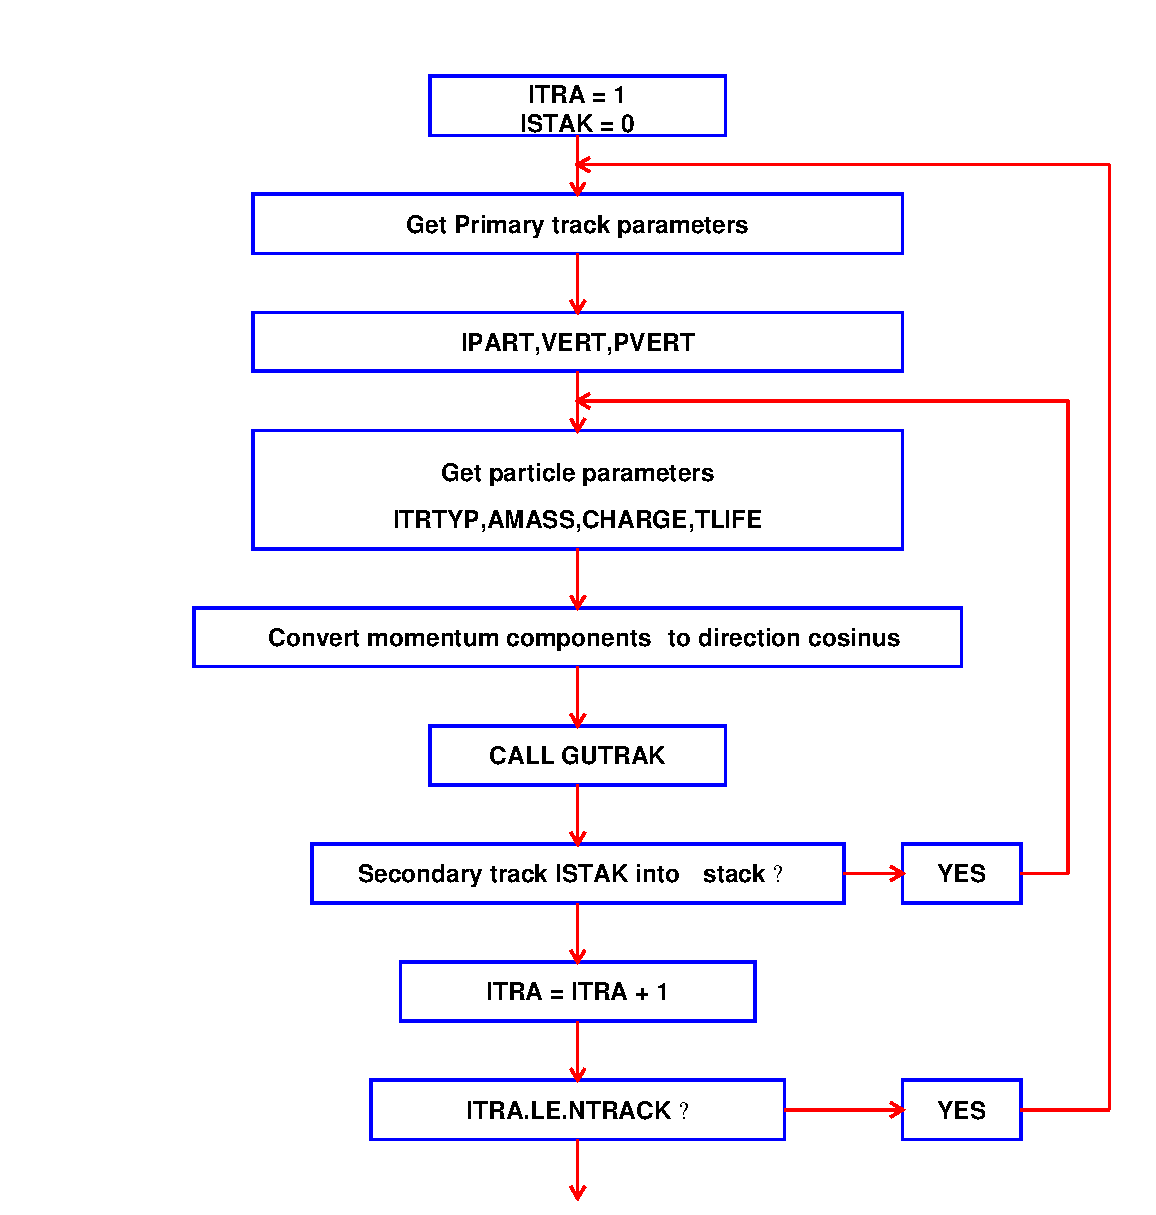
\epsfig{file=eps/trak110-1.eps,width=14cm}
     \caption{{\tt GTREVE} block diagram}
     \label{fg:trak110-1}
\end{figure}

%%%%%%%%%%%%%%%%%%%%%%%%%%%%%%%%%%%%%%%%%%%%%%%%%%%%%%%%%%%%%%%%%%%
%                                                                 %
%  GEANT manual in LaTeX form                              %
%                                                                 %
%  Michel Goossens (for translation into LaTeX)                   %
%  Version 1.00                                                   %
%  Last Mod. Sep 24 1997  1210   MG + IB                          %
%                                                                 %
%%%%%%%%%%%%%%%%%%%%%%%%%%%%%%%%%%%%%%%%%%%%%%%%%%%%%%%%%%%%%%%%%%%
\Origin{R.Brun,F.Bruyant,M.Maire}
\Submitted{01.10.84}    \Revised{16.12.93}
\Version{Geant 3.16}    \Routid{TRAK120}
\Makehead{Steering routine to track one particle}
\Shubr{GTRACK}{}
Controls the tracking at track level.
 
\begin{figure}[hbt]
     \centering
     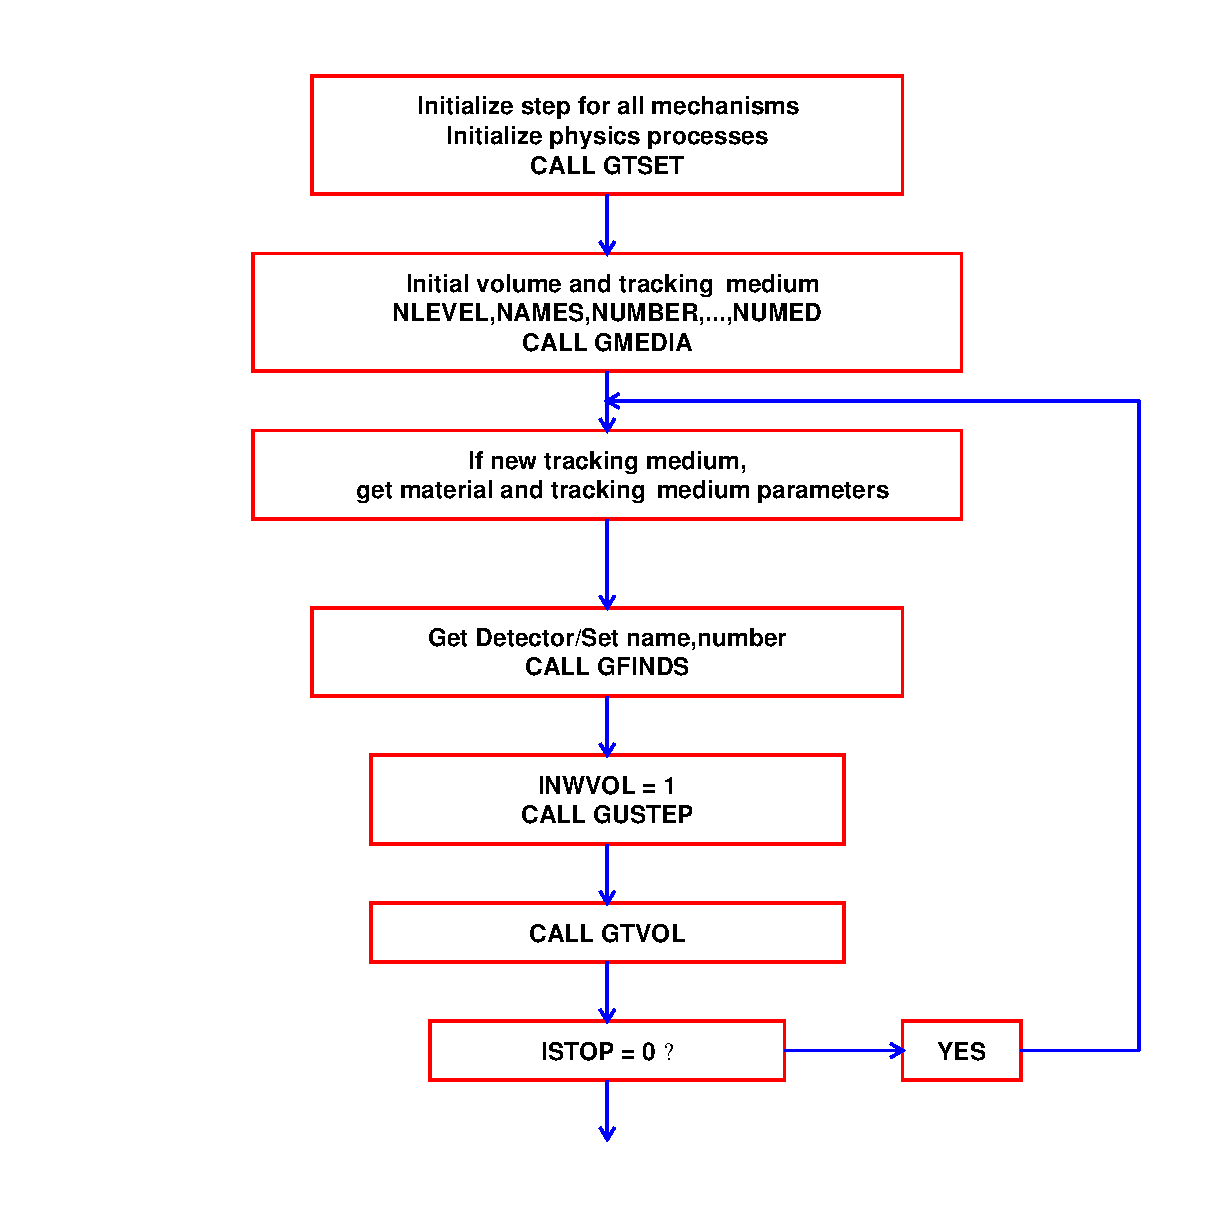
\epsfig{file=eps/trak120-1.eps,width=14cm}
     \caption{{\tt GTRACK} block diagram}
     \label{fg:trak110-1}
\end{figure}

%%%%%%%%%%%%%%%%%%%%%%%%%%%%%%%%%%%%%%%%%%%%%%%%%%%%%%%%%%%%%%%%%%%
%                                                                 %
%  GEANT manual in LaTeX form                              %
%                                                                 %
%  Michel Goossens (for translation into LaTeX)                   %
%  Version 1.00                                                   %
%  Last Mod. Jan 24 1991  1300   MG + IB                          %
%                                                                 %
%%%%%%%%%%%%%%%%%%%%%%%%%%%%%%%%%%%%%%%%%%%%%%%%%%%%%%%%%%%%%%%%%%%
\Authors{R.Brun}        \Origin{R.Brun,F.Bruyant,M.Maire}
\Submitted{01.10.84}    \Revised{16.12.93}
\Version{Geant 3.16}    \Routid{TRAK130}
\Makehead{Tracking one particle through a volume}

\Rind{GTVOL} block diagram.

\begin{figure}[hbt]
     \centering
     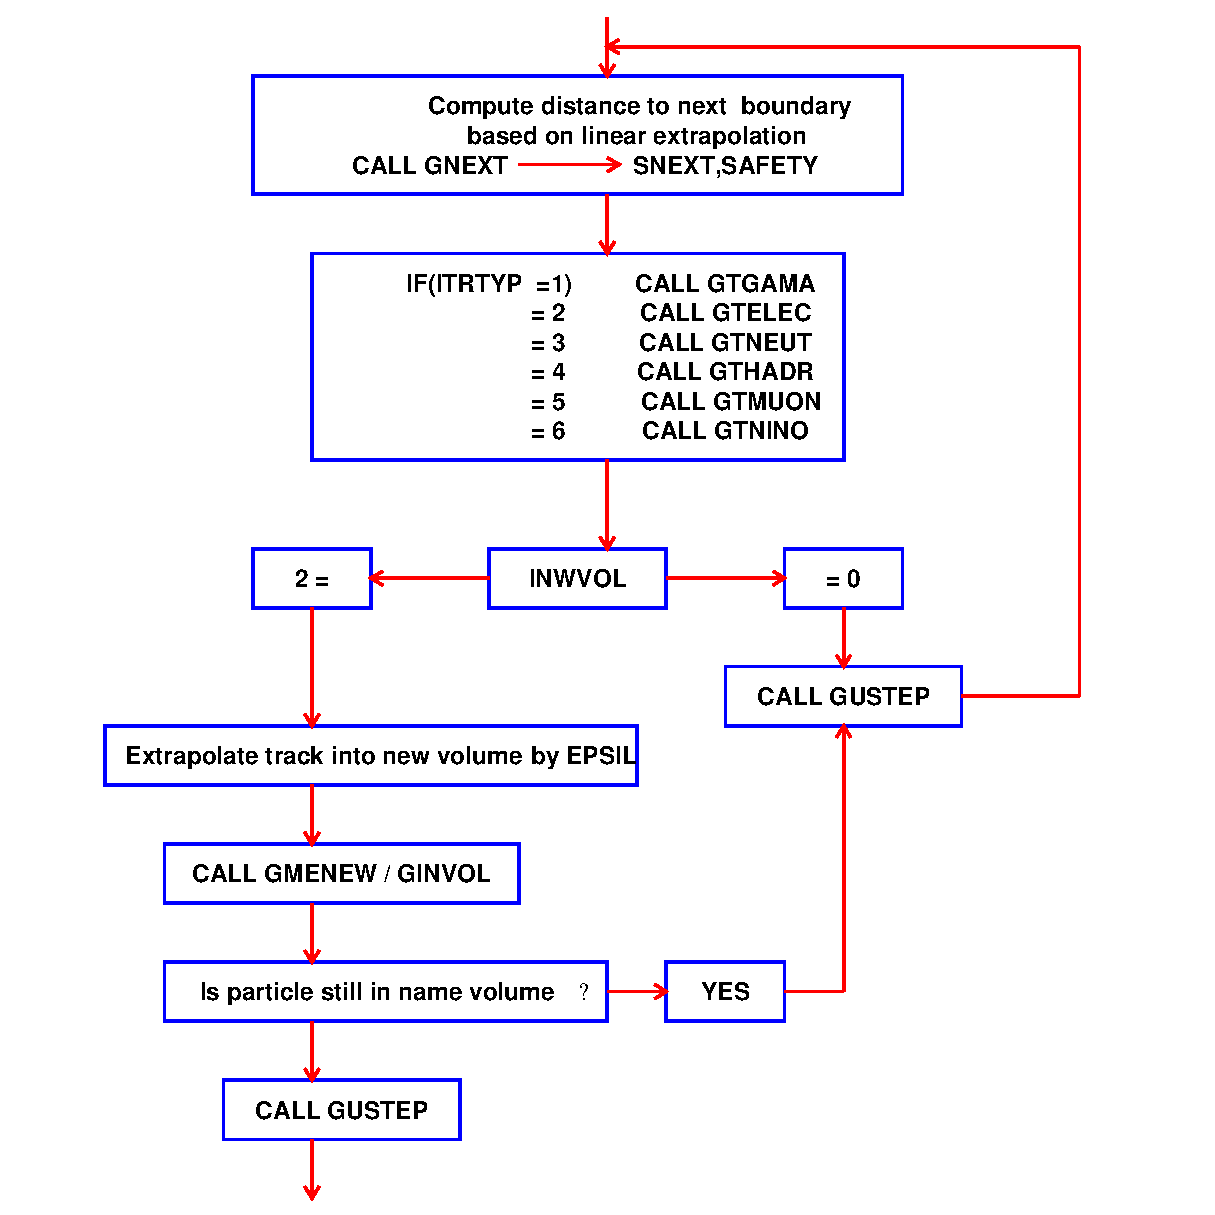
\epsfig{file=eps/trak130-1.eps,width=14cm}
     \caption{Example of geometrical tree structure}
     \label{fg:trak130-1}
\end{figure}

%%%%%%%%%%%%%%%%%%%%%%%%%%%%%%%%%%%%%%%%%%%%%%%%%%%%%%%%%%%%%%%%%%%
%                                                                 %
%  GEANT manual in LaTeX form                              %
%                                                                 %
%  Michel Goossens (for translation into LaTeX)                   %
%  Version 1.00                                                   %
%  Last Mod. Jan 24 1991  1300   MG + IB                          %
%                                                                 %
%%%%%%%%%%%%%%%%%%%%%%%%%%%%%%%%%%%%%%%%%%%%%%%%%%%%%%%%%%%%%%%%%%%
\Origin{R.Brun, M.Maire}
\Revision{F.Carminati, S.Giani, L.Urb\'{a}n}
\Submitted{01.10.84}    \Revised{16.12.93}
\Version{Geant 3.16}    \Routid{TRAK200}
\Makehead{The tracking routines block diagrams}
 
\begin{figure}[hbt]
     \centering
     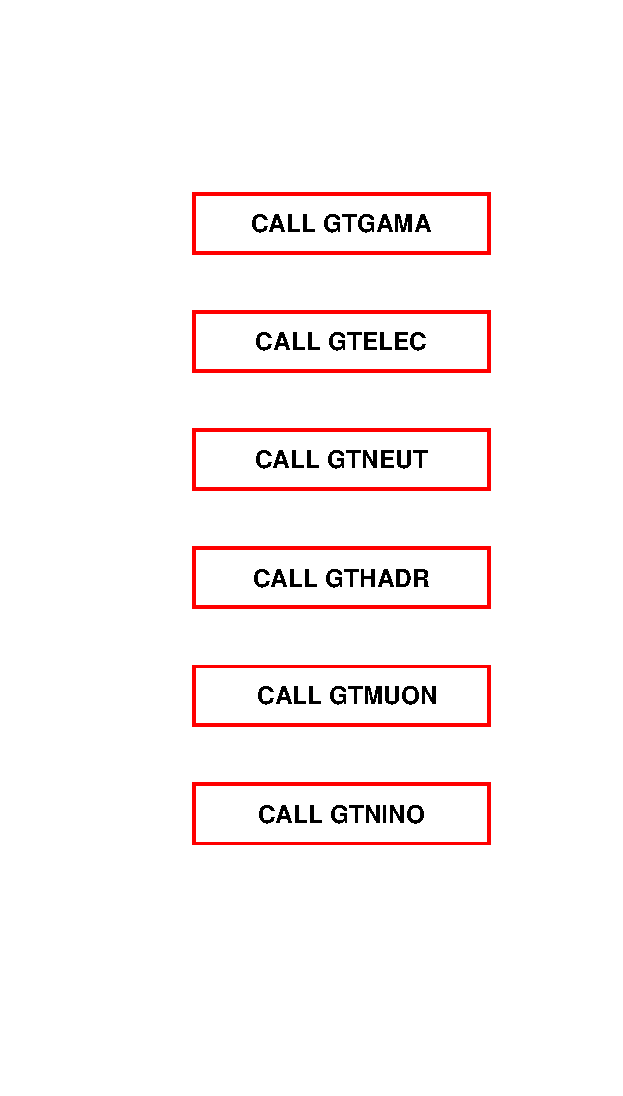
\epsfig{file=eps/trak200-1.eps,width=10cm}
     \caption{The traking routines}
     \label{fg:trak200-1}
\end{figure}

\begin{figure}[hbt]
     \centering
     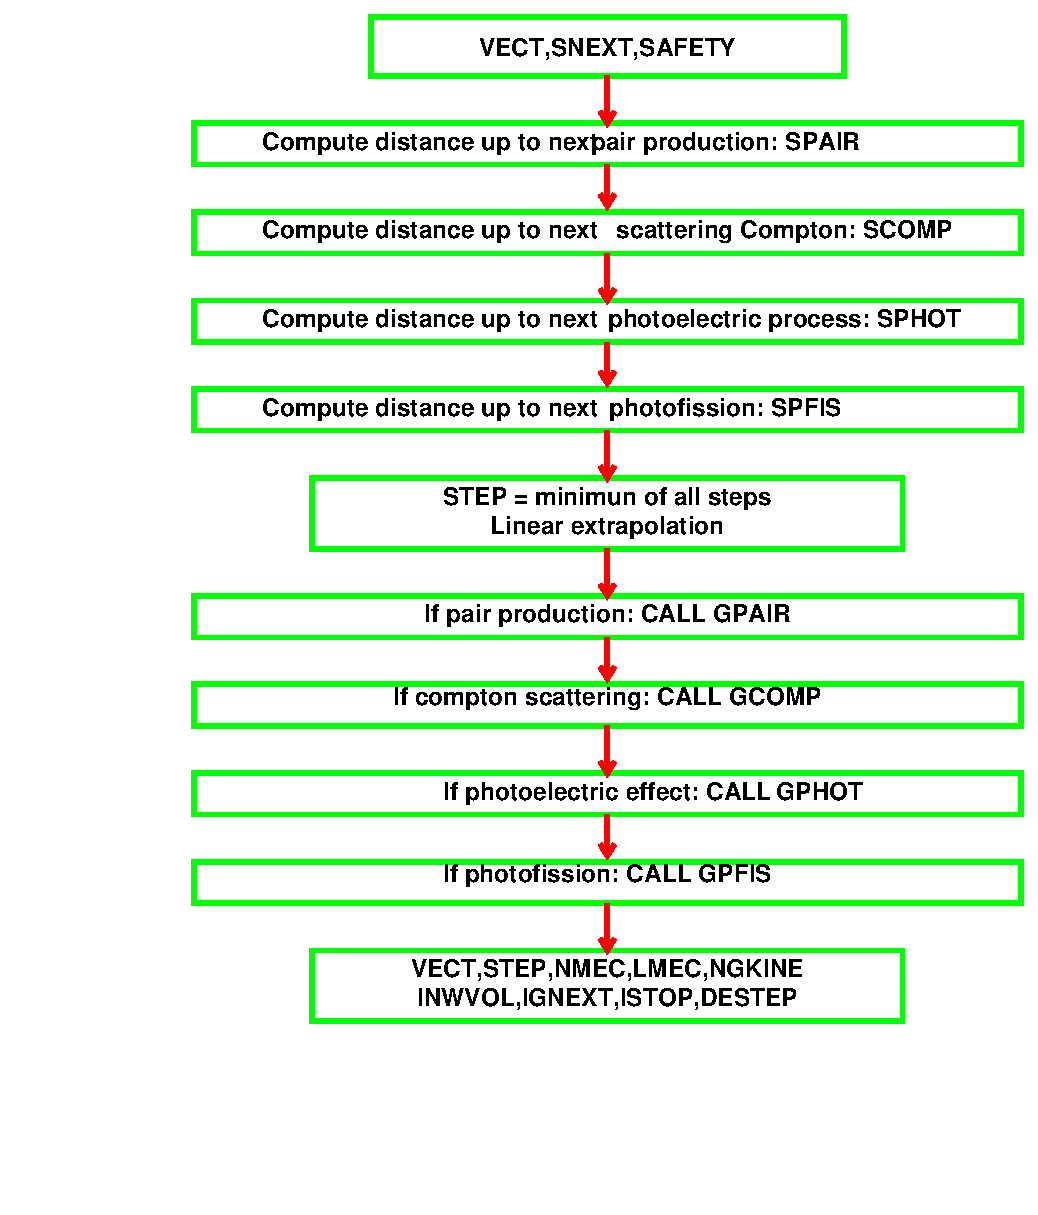
\epsfig{file=eps/trak200-2.eps,width=14cm}
     \caption{{\tt GTGAMA} block diagram}
     \label{fg:trak200-2}
\end{figure}

\begin{figure}[hbt]
     \centering
     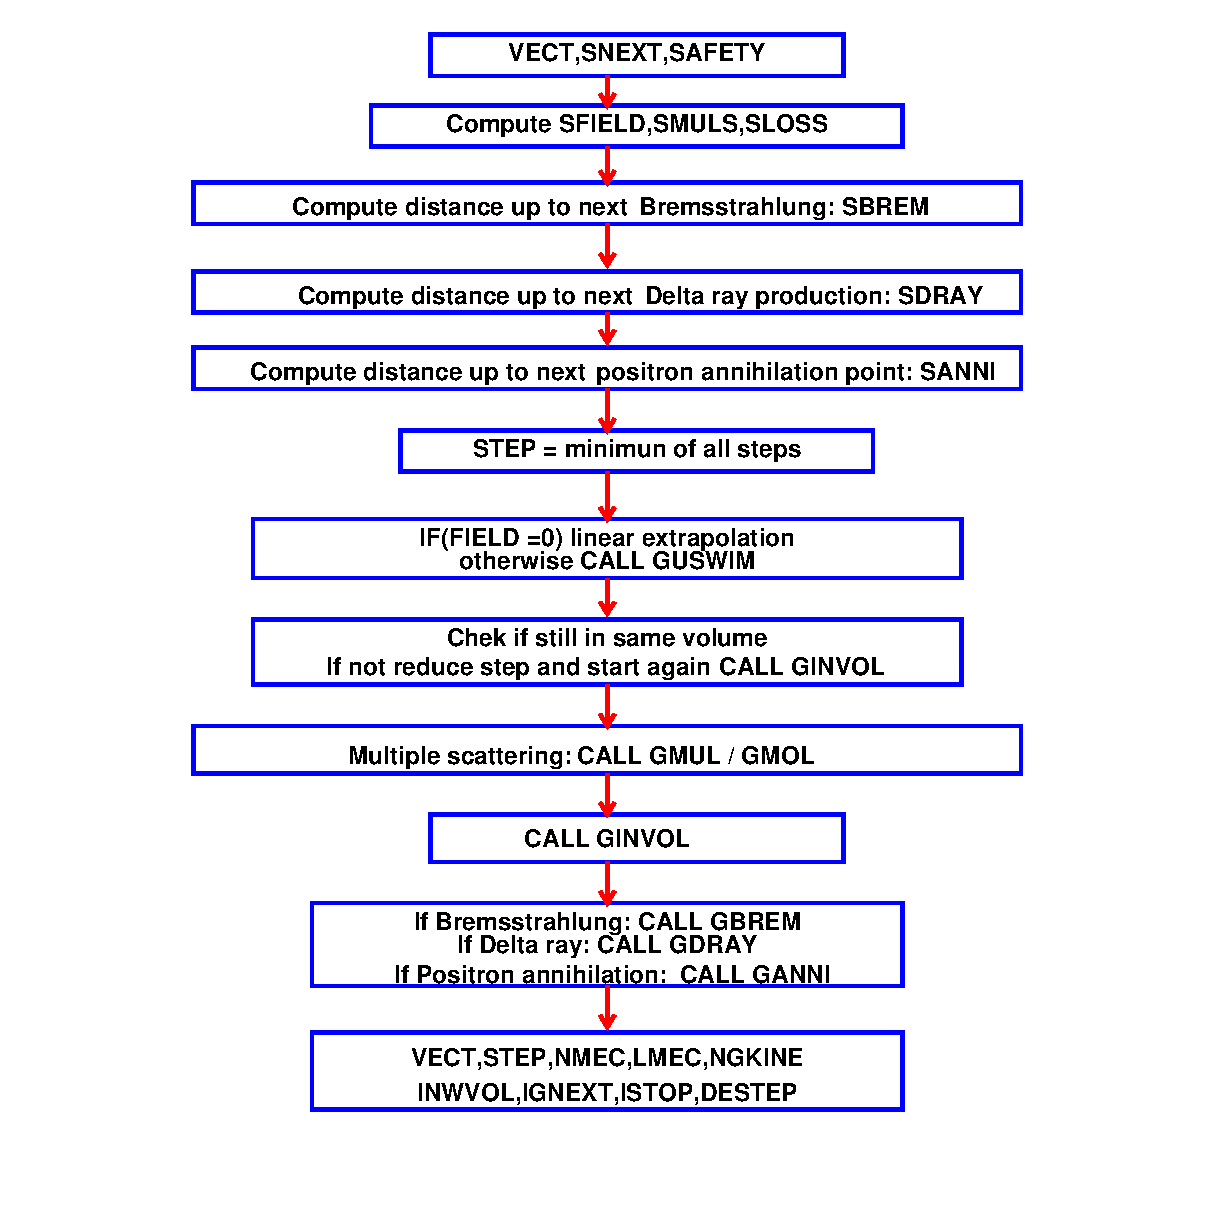
\epsfig{file=eps/trak200-3.eps,width=14cm}
     \caption{{\tt GTELEC} block diagram}
     \label{fg:trak200-3}
\end{figure}

\begin{figure}[hbt]
     \centering
     \epsfig{file=eps/trak200-4.eps,width=14cm}
     \caption{{\tt GTNEUT} block diagram}
     \label{fg:trak200-4}
\end{figure}

\begin{figure}[hbt]
     \centering
     \epsfig{file=eps/trak200-5.eps,width=14cm}
     \caption{{\tt GTHADR} block diagram}
     \label{fg:trak200-5}
\end{figure}

\begin{figure}[hbt]
     \centering
     \epsfig{file=eps/trak200-6.eps,width=14cm}
     \caption{{\tt GTMUON} block diagram}
     \label{fg:trak200-6}
\end{figure}
%
%\begin{figure}[hbt]
%     \centering
%     \epsfig{file=eps/trak200-7.eps,width=14cm}
%     \caption{{\tt GTNINO} block diagram}
%     \label{fg:trak200-7}
%\end{figure}
%
%\begin{figure}[hbt]
%     \centering
%     \epsfig{file=eps/trak200-8.eps,width=14cm}
%     \caption{{\tt GTCKOV} block diagram}
%     \label{fg:trak200-8}
%\end{figure}
%
%\begin{figure}[hbt]
%     \centering
%     \epsfig{file=eps/trak200-9.eps,width=14cm}
%     \caption{{\tt GTHION} block diagram}
%     \label{fg:trak200-9}
%\end{figure}


%%%%%%%%%%%%%%%%%%%%%%%%%%%%%%%%%%%%%%%%%%%%%%%%%%%%%%%%%%%%%%%%%%%
%                                                                 %
%  GEANT manual in LaTeX form                              %
%                                                                 %
%  Michel Goossens (for translation into LaTeX)                   %
%  Version 1.00                                                   %
%  Last Mod. Jan 24 1991  1300   MG + IB                          %
%                                                                 %
%%%%%%%%%%%%%%%%%%%%%%%%%%%%%%%%%%%%%%%%%%%%%%%%%%%%%%%%%%%%%%%%%%%
\Origin{R.Brun}
\Submitted{01.06.83}       \Revised{14.12.93}
\Version{Geant 3.16}       \Routid{TRAK300}
\Makehead{Storing secondary tracks in the stack}

\Shubr{GSKING}{(IT)}
\begin{DLtt}{MMMMMMMM}
\item[IT] ({\tt INTEGER}) number of the track to be stored for subsequent
tracking, if {\tt IT=0} all secondary tracks generated in the current
step are stored for tracking.
\end{DLtt}

During transport, particles can generate new particles, called 
secondary. In {\tt GEANT} these particles are stored in the common
\FCind{/GCKING/} (see {\tt [BASE030]} for an explanation of the
variables in this common). The number of particles generated in
the current step is {\tt NGKINE} (common \FCind{/GCKING/}). If no
user action is taken, the variable {\tt NGKINE} is reset to 0 at the
beginning of the subsequent step and these particles are not transported.

To be transported by {\tt GEANT}, these particles need to be stored
in the data structure {\tt JSTAK} (see {\tt [TRACK399]}) which
normally is a
LIFO stack: the last particle generated is the first one to be
tracked when the current one stops. The order of tracking can be changed 
by the user, plase see {\tt [TRAK310]} for more information on this
subject. 

The routine \Rind{GSKING} moves particles from the \FCind{/GCKING/} common
to the {\tt JSTAK} structure, where {\tt GEANT} looks for particles to 
transport.

When a particle is fetched from the {\tt JSTAK} data structure, its place
is freed for a new one, so the information on the initial kinematics of
this track is lost. It may be useful in some occasion to record the initial
kinematic of a track and save it till the end of the event. This is accomplished
by storing the particle information both in the {\tt JSTAK} data structure
and in the {\tt JVERTX/JKINE} one, which is permanent throughout the life
of the event. As already said in {\tt [KINE100]}, this should not be done
by the user calling directly the \Rind{GSVERT}/\Rind{GSKINE} routines
during tracking, but rather controlling the action of \Rind{GSKING} via
the array {\tt IFLGK} in common \FCind{/GCKING/}. If the particle number
{\tt IG} generated in the current step ({\tt 1} $\leq$ {\tt IG} $\leq$ 
{\tt NGKINE}) is being moved to the {\tt JSTAK} {\it stack}, either
singularly or together with all the other particles generated in the
current step (setting the argument of \Rind{GSKING} to 0), the action
performed depends on {\tt IFLGK(IG)}:

\begin{DLtt}{MMMMMMMMMMMM}
\item[IFLGK(IG)$<$0] the particle is ignored;
\item[~~~~~~~~~$=$0] the particle is stored on the temporary stack {\tt JSTAK}
to be transported;
\item[~~~~~~~~~$=$1] the particle is stored on the temporary stack {\tt JSTAK}
to be transported {\it and} in the {\tt JKINE} data structure attaching it to
a vertex created in the current position (array {\tt VECT(I), I}=1,3 in the
\FCind{/GCTRAK/} common);
\item[~~~~~~~~~$>$1] the particle is stored on the temporary stack {\tt JSTAK}
to be transported {\it and} in the {\tt JKINE} data structure attaching it to
vertex number {\tt IFLGK(IG)}, which must exist.
\end{DLtt}

If {\tt IFLGK(IG)}$>$0, after the call to \Rind{GSKING}, {\tt IFLGK(IG)} is
set to the newly created track number in {\tt JKINE}. The number of the
vertex used is returned in {\tt IFLGK(NGKINE+1)}. This feature allows the
user to identify the created vertex and tracks via the routines 
\Rind{GSVERU} and \Rind{GSKINU} (see {\tt [KINE100]}).

\section*{Example}

In case of a hadronic interaction, discard the neutrinos, store the protons
in the permanent data structure {\tt JVERTX/JKINE}, and store all the
other particles produced in the temporary stack.

Add to the protons in the {\tt JKINE} bank the {\tt JVOLUM}
and copy number of the 
volume and the number of the tracking medium where they have been produced
by an interaction.

\begin{verbatim}
      SUBROUTINE GUSTEP
+SEQ,GCKING,GCVOLU,GCTMED.
      CHARACTER*4 CHCASE
      DIMENSION UBUF(3)
      .
      .
      .
      CALL UHTOC(KCASE,4,CHCASE,4)
      IF(CHCASE.EQ.'HADR') THEN
         DO 10 IG=1, NGKINE
            IPART = GKIN(5,IG)
            IF(IPART.EQ.4) THEN
*---                Discard neutrinos
               IFLGK(IG)=-1
            ELSEIF(IPART.EQ.14) THEN
*---                Save protons in JKINE and transport them
               IFLGK(IG)=1
            ELSE
*---                Simply transport the rest
               IFLGK(IG)=0
            ENDIF
  10     CONTINUE
      ENDIF
*---                Perform action on all the particles
      CALL GSKING(0)
*---               Add information to the JKINE bank
      DO 20 IG=1,NGKINE
         IPART = GKIN(5,IG)
         IF(IPART.EQ.14) THEN
*---               This is a proton
*---               Get the track number
            IT = IFLGK(IG)
            NUBUF = 3
            UBUF(1) = LVOLUM(NLEVEL)
            UBUF(2) = NUMBER(NLEVEL)
            UBUF(3) = NUMED
            IADR = 0
*---               Store the information
            CALL GSKINU(IT,NUBUF,UBUF,IADR)
         ENDIF
  20  CONTINUE
\end{verbatim}

%%%%%%%%%%%%%%%%%%%%%%%%%%%%%%%%%%%%%%%%%%%%%%%%%%%%%%%%%%%%%%%%%%%
%                                                                 %
%  GEANT manual in LaTeX form                              %
%                                                                 %
%  Michel Goossens (for translation into LaTeX)                   %
%  Version 1.00                                                   %
%  Last Mod. Jan 24 1991  1300   MG + IB                          %
%                                                                 %
%%%%%%%%%%%%%%%%%%%%%%%%%%%%%%%%%%%%%%%%%%%%%%%%%%%%%%%%%%%%%%%%%%%
\Origin{F.Carminati}
\Submitted{14.12.93}       \Revised{14.12.93}
\Version{Geant 3.16}       \Routid{TRAK310}
\Makehead{Altering the order of tracking secondary particles}

When secondary particles are produced during particle transport, if
the user wants to transport them in turn, they must be stored by
a call to \Rind{GSKING} or \Rind{GSKPHO} onto the temporary stack
{\tt JSTAK}. As explained in {\tt [TRAK310]}, this is a LIFO
structure, where the last particle introduced is the first to be extracted
to be transported. It may be sometimes interesting to alter the order
of tracking, for instance to decide whether the current event is
worth completing or whether it should be skipped to go to next one.

It is possible in {\tt GEANT} to alter the behaviour of the {\tt JSTAK}
structure using one of the words of the stack, normally reserved for
the user. Stack ordering is activated via the data record {\tt SORD 1}.
This will set to 1 the variable {\tt ISTORD} in common \FCind{/GCSTAK/},
which is by default initialised to 0.

When stack ordering is activated, the routine \Rind{GLTRAC}, which
fetches the next particle to be tracked from {\tt JSTAK}, instead
of the last one, will select the one with the maximum value of the
user word. This user word must be set by the user in the variable
{\tt UPWGHT} in the common \FCind{/GCTRAK/} prior to the call to
\Rind{GSKING} to store each secondary.

If, for instance, all the protons must be tracked first, in order of
production, and all the other particles after, again according to their
time of production, the following code should appear in \Rind{GUSTEP}:

\begin{verbatim}
      SUBROUTINE GUSTEP
+SEQ,GCTRAK,GCKING
      .
      .
      .
      DO 10 IG=1,NGKINE
*---         Younger particles tracked first
*---         Add to the current time of flight the time delay of
*---         the secondary
         UPWGHT = -TOFG-TOFD(IG)
         IPART = GKIN(5,IG)
         IF(IPART.EQ.14) THEN
*---         This is a proton, add a 100 microseconds to have it
*---         tracked first
            UPWGHT = UPWGHT+1E-4
         ENDIF
*---         Now store the particle in the GEANT stack
         CALL GSKING(IG)
  10  CONTINUE
\end{verbatim}

Users should be aware of the fact that ordering the stack will change the
results, because transport depends on random numbers which will be different
for the same particle in the two cases.

%%%%%%%%%%%%%%%%%%%%%%%%%%%%%%%%%%%%%%%%%%%%%%%%%%%%%%%%%%%%%%%%%%%
%                                                                 %
%  GEANT manual in LaTeX form                              %
%                                                                 %
%  Michel Goossens (for translation into LaTeX)                   %
%  Version 1.00                                                   %
%  Last Mod. Jan 24 1991  1300   MG + IB                          %
%                                                                 %
%%%%%%%%%%%%%%%%%%%%%%%%%%%%%%%%%%%%%%%%%%%%%%%%%%%%%%%%%%%%%%%%%%%
\Origin{R.Brun}
\Revision{F.Carminati}
\Submitted{01.11.83} \Revised{14.12.93}
\Version{Geant 3.16}\Routid{TRAK399}
\Makehead{The temporary stack data structure JSTAK}

\begin{figure}[hbt]
     \centering
     \epsfig{file=eps/trak399-1.eps,width=14cm}
     \caption{Layout of the temporary stack data structure {\tt JSTAK}}
     \label{fg:trak399-1}
\end{figure}
The {\tt JSTAK} bank is filled by \Rind{GSKING}.

%%%%%%%%%%%%%%%%%%%%%%%%%%%%%%%%%%%%%%%%%%%%%%%%%%%%%%%%%%%%%%%%%%%
%                                                                 %
%  GEANT manual in LaTeX form                              %
%                                                                 %
%  Michel Goossens (for translation into LaTeX)                   %
%  Version 1.00                                                   %
%  Last Mod. Jan 24 1991  1300   MG + IB                          %
%                                                                 %
%%%%%%%%%%%%%%%%%%%%%%%%%%%%%%%%%%%%%%%%%%%%%%%%%%%%%%%%%%%%%%%%%%%
\Origin{R.Brun}
\Submitted{01.06.83}        \Revised{15.12.93}
\Version{Geant 3.10}        \Routid{TRAK400}
\Makehead{Handling of track space points}

\Shubr{GSXYZ }{}
Stores the position of the current particle from common \FCind{/GCTRAK/} into
the data structure {\tt JXYZ}.
 
\Shubr{GPJXYZ}{(NUMB)}
 
\begin{DLtt}{MMMMMMMM}
\item[NUMB] ({\tt INTEGER}) track number, all tracks if =0;
\end{DLtt}
Prints space points stored in the data structure {\tt JXYZ}
for track number {\tt NUMB}.
 
\Shubr{GPCXYZ}{}
Prints tracking and physics parameters after
the current step. This routine can be called from \Rind{GUSTEP}.
 
Some of these routines are called by \Rind{GDEBUG}, see {\tt [BASE400]}
for more information.

%%%%%%%%%%%%%%%%%%%%%%%%%%%%%%%%%%%%%%%%%%%%%%%%%%%%%%%%%%%%%%%%%%%
%                                                                 %
%  GEANT manual in LaTeX form                              %
%                                                                 %
%  Michel Goossens (for translation into LaTeX)                   %
%  Version 1.00                                                   %
%  Last Mod. Jan 24 1991  1300   MG + IB                          %
%                                                                 %
%%%%%%%%%%%%%%%%%%%%%%%%%%%%%%%%%%%%%%%%%%%%%%%%%%%%%%%%%%%%%%%%%%%
\Origin{R.Brun}
\Submitted{01.11.83}    \Revised{15.12.93}
\Version{Geant 3.16}    \Routid{TRAK499}
\Makehead{The space point data structure JXYZ}

\begin{figure}[hbt]
     \centering
     \epsfig{file=eps/trak499-1.eps,width=14cm}
     \caption{Layout of the {\tt JXYZ} data structure}
     \label{fg:trak499-1}
\end{figure}

{\tt JX=LQ(JXYZ-ITRA)} is the pointer to the space points of track number 
{\tt ITRA}
 
The space point banks {\tt JXYZ} are only used for debug and display
purposes. They can be filled by using the routine \Rind{GSXYZ} from
\Rind{GUSTEP}. The drawing routine \Rind{GDXYZ}
gets the space coordinates from {\tt JXYZ}.

%%%%%%%%%%%%%%%%%%%%%%%%%%%%%%%%%%%%%%%%%%%%%%%%%%%%%%%%%%%%%%%%%%%
%                                                                 %
%  GEANT manual in LaTeX form                                     %
%                                                                 %
%  Michel Goossens (for translation into LaTeX)                   %
%  Version 1.00                                                   %
%  Last Mod. Jan 24 1991  1300   MG + IB                          %
%                                                                 %
%%%%%%%%%%%%%%%%%%%%%%%%%%%%%%%%%%%%%%%%%%%%%%%%%%%%%%%%%%%%%%%%%%%
\Origin{R.Brun, M.Hansroul}
\Submitted{01.10.81}   \Revised{16.12.93}
\Version{Geant 3.16}   \Routid{TRAK500}
\Makehead{Tracking routines in magnetic field}

\Shubr{GUSWIM}{(CHARGE,STEP,VECT,VOUT*)}
\begin{DLtt}{MMMMMMMM}
\item[CHARGE] ({\tt REAL}) particle charge in $e$ unit;
\item[STEP] ({\tt REAL}) step size in cm;
\item[VECT] ({\tt REAL}) array of 7 with the initial coordinates, direction 
cosines and momentum ($x$, $y$, $z$, $p_x/p$, $p_y/p$, $p_z/p$, $p$);
\item[VOUT] ({\tt REAL}) array of 7 with the final coordinates, direction 
cosines and momentum after the step.
\end{DLtt}
 
This is the steering routine for calculating the deviation of a charged
particle in magnetic field. It is called by the {\tt GEANT} tracking 
routines: \Rind{GTELEC}, \Rind{GTHADR}, \Rind{GTMUON} and \Rind{GTHION}.
Even if this routine follows the naming conventions of the user routines,
the version provided in the {\tt GEANT} library is quite adequate for most
situation, and users should have a very good reason to modify it.
 
It calls \Rind{GRKUTA}, \Rind{GHELIX}, \Rind{GHELX3} according to the value
1, 2 or 3 of {\tt IFIELD} in common \FCind{/GCTMED/}. {\tt IFIELD} correspond
to the argument to the \Rind{GSTMED} routine (see {\tt [CONS200]}).
{\tt IFIELD = -1} is reserved for user decision in case \Rind{GUSWIM}
is modified by the user.

\Shubr{GHELX3}{(FIELD,STEP,VECT,VOUT*)}

\begin{DLtt}{MMMMMMMM}
\item[FIELD] ({\tt REAL}) field value in kilo-Gauss multiplied by 
the charge of the particle in $e$ units;
\item[STEP] ({\tt REAL}) step size in cm;
\item[VECT] ({\tt REAL}) array of 7, same as for \Rind{GUSWIM};
\item[VOUT] ({\tt REAL}) array of 7, same as for \Rind{GUSWIM};
\end{DLtt}

Transport the particle by a length {\tt STEP} in a magnetic
field. The field is assumed to be uniform and parallel to the
$z$ axis. The value of the field is the {\tt FIELDM} argument to
the \Rind{GSTMED} routine (see {\tt [CONS200]}). The particle is
transported along an helix.  The call to this routine is selected by 
\Rind{GUSWIM} when {\tt IFIELD=3} in the call to \Rind{GSTMED}.

\Shubr{GHELIX}{(CHARGE,STEP,VECT,VOUT*)}

\begin{DLtt}{MMMMMMMM}
\item[CHARGE] ({\tt REAL}) particle charge in $e$ units;
\item[STEP] ({\tt REAL}) step size in cm;
\item[VECT] ({\tt REAL}) array of 7, same as for \Rind{GUSWIM};
\item[VOUT] ({\tt REAL}) array of 7, same as for \Rind{GUSWIM};
\end{DLtt}
 
Transport the particle by a length {\tt STEP} in a magnetic
field. The magnetic field is calculated in the middle of the step
(along a straight line) and it is supposed to be constant along
the step and the particle is transported along an helix. 
The call to this routine is selected by
\Rind{GUSWIM} when {\tt IFIELD=2} in the call to \Rind{GSTMED}.
This routine is intended for magnetic fields with a small gradient.
The value of the field is obtained from the routine \Rind{GUFLD}
which must be coded by the user.

\Shubr{GRKUTA}{(CHARGE,STEP,VECT,VOUT*)}
 
The arguments have the same meaning than those of
\Rind{GHELIX}. Transport a particle in magnetic field using
Runge-Kutta method for solving the kinematic equations (Nystroem 
algorithm~\cite{bib-NATB}, procedure 25.5.20).
The call to this routine is selected by
\Rind{GUSWIM} when {\tt IFIELD=1} in the call to \Rind{GSTMED}.
This method is the slower of the three and it must be used for
magnetic fields with strong gradient. Again the magnetic field is
obtained from the \Rind{GUFLD} routine which the user has to code.

\Shubr{GUFLD}{((VECT,F*)}

\begin{DLtt}{MMMMMMMM}
\item[VECT] ({\tt REAL}) array of 3 with the position in space where the
field has to be returned;
\item[F] ({\tt REAL}) array of 3 with the magnetic field in {\tt VECT},
in kilo-Gauss units.
\end{DLtt}

User routine to return the three components of the magnetic field at
point {\tt VECT} expressed in kilo-Gauss. This routine must be provided
by the user for all tracking media where {\tt IFIELD} is 1 or 2. This
routine will be called very often, at least three times at each step,
so all the care must be put in its optimisation.

\putbib[cnasbibl,geabibl]
\end{bibunit}
 
%%     XINT part     %%
 
\begin{bibunit}[unsrt]
\renewcommand{\bibname}{XINT Bibliography}
%%%%%%%%%%%%%%%%%%%%%%%%%%%%%%%%%%%%%%%%%%%%%%%%%%%%%%%%%%%%%%%%%%%
%                                                                 %
%  GEANT manual in LaTeX form                              %
%                                                                 %
%  Michel Goossens (for translation into LaTeX)                   %
%  Version 1.00                                                   %
%  Last Mod. Jan 24 1991  1300   MG + IB                          %
%                                                                 %
%%%%%%%%%%%%%%%%%%%%%%%%%%%%%%%%%%%%%%%%%%%%%%%%%%%%%%%%%%%%%%%%%%%
\Documentation{R.Brun}
\Submitted{15.06.84}   \Revised{19.12.93}
\Version{Geant 3.16}    \Routid{XINT001}
\Makehead{The interactive version of GEANT}
 
The interactive version is an essential tool for users who are
in charge of the design of a detector.
In addition to all the batch tools which are also available, the
interactive user can call one by one and in any order all the basic
functions of {\tt GEANT} to:
\begin{itemize}
\item design or modify the geometry of the setup;
\item exploit the drawing package in a more efficient way;
\item change the running conditions on a event by event basis.
\end{itemize}
The system is based on the {\tt KUIP}~\cite{bib-KUIP}
command processor.
The user has to know a minimum about {\tt KUIP} and should read
at least the first chapter of the manual.

A set of encapsulated Postscript files have been collected in
a new section XINT010. They illustrate the visualization possibilities
of the interactive version of {\tt GEANT}. 

\section{Invoking the interactive version}
Instead of writing a MAIN program to initialize the Geant batch
version, it is possible to use the MAIN interactive program (GXINT321.F)
provided in /cern/pro/lib exactly as the library LIBGEANT321.A. The user
has simply to insert in his link file the file GXINT321.F as the main
program, followed by the user object code and by the library LIBGEANT321.A.
\\[.5em] Example: \\[.1em]
       PROGRAM GXINT \\[.1em]
* \\[.1em]
*     GEANT main program. To link with the MOTIF user interface \\[.1em]
*     the routine GPAWPP(NWGEAN,NWPAW) should be called, whereas \\[.1em]
*     the routine GPAW(NWGEAN,NWPAW) gives access to the basic \\[.1em]
*     graphics version. \\[.1em]
* \\[.1em]
      PARAMETER (NWGEAN=3000000,NWPAW=1000000) \\[.1em]
      COMMON/GCBANK/GEANT(NWGEAN) \\[.1em]
      COMMON/PAWC/PAW(NWPAW) \\[.1em]
* \\[.1em]
      CALL GPAWPP(NWGEAN,NWPAW) \\[.1em]
* \\[.1em]
      END \\[.5em]
The user has to set the desired value of NWGEAN and NWPAW for the
GEANT and PAW Zebra stores, and to call the desired initialization routine:
\begin{itemize}
\item GPAW to initialize, besides GEANT, also HIGZ and to include the full
      functionality of PAW;
\item GPAWPP to initialize, besides GEANT and HIGZ, also the Motif version 
      and to include the full functionality of Paw++;
\item USER initialization routine, to do anything else (for example a UGINIT-
      like routine or a gxint315.f--like routine). 
\end{itemize}
The interactive version, after the initialization, gives the control to the
user at the prompt GEANT $>$ ; then it is possible to type and execute 
commands (corresponding to batch routines) to edit the geometry, the materials
or the tracking media at run time. It is also possible to execute commands
to visualize the detectors, to set the kinematics and to run events. Again
interactively, one can spy the histograms, change the kinematics, and run
more events (visualizing the tracks and the hits, for example). The GXINT
chapter contains in the following pages a full description of the available
GEANT commands. See the PAW, KUIP, DZDOC, HIGZ manuals for a description of
the relative commands executable from GEANT. All the commands are also
documented by an on-line help. (Try to type HELP at the first GEANT $>$ prompt).
In the interactive version, a COMIS interface is also available: COMIS is a
FORTRAN interpreter which allows:
\begin{itemize}
\item to edit at run time important routines like UGEOM, GUSTEP, GUKINE, etc.
\item to `execute' them from the interactive session, without having to 
      recompile and relink, by typing commands like CALL UGEOM.F.
\end{itemize}
Of course the interpreter is slower than the compiled object code,
then, since GEANT321, it is also possible to invoke the native compiler and
to link dinamically to the executable the compiled routine (see the COMIS 
manual for further details).


The following write ups describe individual commands which can be typed
one by one at the terminal, or grouped into macros which can be edited
and saved in the {\tt KUIP} environment.

The commands are listed in subsection 1 - 13:

\begin{center}\begin{tabular}{ll}
1. &  General GEANT \\
2. & Clipping commands GEANT/CVOL \\
3. & Drawing commands GEANT/DRAWING \\
4. & Graphics control commands GEANT/DRAWING \\
5. & Geometry commands GEANT/GEOMETRY \\
6. & Volume creation commands GEANT/CREATE \\
7. & Control commands GEANT/CONTROL \\
8. & ZEBRA/RZ commands GEANT/RZ \\
9. & ZEBRA/FZ commands GEANT/FZ \\
10. & Data structure commands GEANT/DZ \\
11. & Scanning commands GEANT/SCAN \\
12. & Physics parameter commands GEANT/PHYSICS \\
13. & List commands GEANT/LISTS \\
\end{tabular}\end{center}

\section{The Motif Interface}
The interactive version 3.21 contains an object oriented Motif-based user
interface. It can be accessed specifying `m' as workstation type.
The full functionality of the X11 version remains available, while new 
Motif-specific features have been added. \\[1em]
\section{The main ideas} 
The {\tt GEANT} data structures are 
considered as KUIP browsable classes and their
contents as `objects' on which one can perform actions 
(the {\tt GEANT} commands).
According to the Motif conventions, an object can be selected clicking the
left button of the mouse (when the cursor is on the icon representing that
object). Clicking then on the right button of the mouse, a menu of possible
commands will appear (double clicking on the left button the first action of
this list will be executed); 
the selected command will perform the relative actions
on the selected object. Such actions (like drawing, for example) can be
executed either directly or via the use of an automatically opened Motif panel.
Objects drawn in the graphics window can be `picked' as well (for example,
volumes, tracks, hits); clicking the right button when the cursor is on the
selected object, a menu of possible actions on that object is displayed.
Users can finally define Motif panels containing buttons corresponding to the
most frequently used commands. An on-line help is available for any specific
subject. \\[1em]

\section {The Geant++ Executive Window}
It replaces the normal dialog window; it contains a Transcript Pad, where the
text output of the executed commands is displayed, and an Input Pad, where the
user can still type the desired commands in the old style. \\[1em]
The {\tt Geant++} Main File Browser \\[1em]
On the left side it displays a list of the {\tt GEANT} data structures, of the 
available commands, file, macros and Zebra divisions used. Selecting one of
them, the full list of icons representing the objects of that class is shown
in the main area of the browser. Proceeding as described before, it is 
possible to perform actions on the classes (like create a new object) or on
the objects belonging to them. It is possible to create menus of commands
just clicking on the string `commands' at the top line of the browser. \\[1em]
The Geant++ Graphics Window \\[1em]
Any object to be drawn in the graphics window can be stored in the current
picture file (automatically opened after each NEXT command) via a call to 
IGPID (see Higz manual). It can be afterwards `picked' as described before.
In the case of commands executed via the use of Motif panels, some input values
can be set with a slider ranging in the specifed range for the relative
variable; moving the slider (after having clicked on the right-hand `activating
box') the relative action is performed in the graphics
window when releasing the button of the mouse; when in `drag mode', the 
action is performed {\it while} moving the slider (keeping the left button
pressed): especially when double buffering has been selected, this can be
useful for real time manipulations.\\[1em]
\section {An Example}
Start your {\tt GEANT321} executable module 
(linked with GXINT321 and Motif1.2);
\\[.5em] type `m' as workstation type;
\\[.5em] click the left button of the mouse after positioning the cursor on the 
string VOLU in the browser;
\\[.5em] click the left button of the mouse after positioning the cursor on 
any icon in the main area of the browser;
\\[.5em] click now the right button of the mouse and keep it pressed;
\\[.5em] move the mouse to select the action `Tree' and release the button;
\\[.5em] the drawing of the logical tree will be displayed in the graphics
window;
\\[.5em] position the cursor on the drawing of a box (containing a volume name)
in the graphics window, click the right button and keep it pressed;
\\[.5em] release the button selecting the action `Dspec';
\\[.5em] the command DSPEC for that volume will be executed in a separate
window;
\\[.5em] repeat the exercise selecting this time the action `Dspe3d';
\\[.5em] the DSPEC will be executed in the first window, the volume 
specifications will be printed in a separate window and a Motif panel will
appear;
\\[.5em] click the left button of the mouse positioning the cursor in the Motif
panel on the `Value changed' button, and select the DRAG option;
\\[.5em] click now the left button on the `activating box' on the right of
the `Theta' slider;
\\[.5em] click on the `Theta' slider and, keeping pressed the left button of the
mouse, move it right-wards;
\\[.5em] the drawing in the graphics window will rotate;
\\[.5em] release the button and type `igset 2buf 1' in the executive window;
\\[.5em] restart moving the slider as before. 

	%%%%%%%%%%%%%%%%%%%%%%%%%%%%%%%%%%%%%%%%%%%%%%%%%%%%%%%%%%%%%%%%%%%
%                                                                 %
%  GEANT manual in LaTeX form                                     %
%                                                                 %
%  Version 1.00                                                   %
%                                                                 %
%  Last Mod. 15 June 1993 19:00  MG                               %
%                                                                 %
%%%%%%%%%%%%%%%%%%%%%%%%%%%%%%%%%%%%%%%%%%%%%%%%%%%%%%%%%%%%%%%%%%%
\Authors{S.Giani}     \Origin{Same}
\Submitted{15.06.84}   \Revised{20.03.94}
\Version{Geant 3.21}\Routid{XINT002}
\Makehead{Introduction to the Interactive version of GEANT}

\newif\ifMENUtext \MENUtexttrue
\newcommand{\DEFMENU}[3]{% {level}{name}{path}
\section{#3}}

\newcommand{\INDEX}[1]{% protect underscores
{\def\_{\char'137}\index{#1@{\tt #1}}}}

\newcommand{\DEFCMD}[5]{% {menulabel}{cmdlabel}{menupath}{cmdname}{args}
\par%\begin{minipage}{\textwidth}
\subsection{#4 #5 \label{#1:#2}\INDEX{#3/#4}\INDEX{#4}}}
\newcommand{\ENDCMD}{\par}%\end{minipage}\par}

\newcommand{\DEFCBIG}[5]{% DEFCMD with long guidance text
\subsection{#4 #5 \label{#1:#2}\INDEX{#3/#4}\INDEX{#4}}}
\newcommand{\ENDCBIG}{\par}

\newcommand{\BEGARG}{%
\par\begin{longtable}{lcp{.75\textwidth}}\endhead}
\newcommand{\DEFARG}[4]{% {parname}{partype}{prompt}{default}
{\tt #1} & #2 & ``#3'' {\tt #4} \\}
\newcommand{\ENDARG}{%
\end{longtable}\par}

\newcommand{\BEGOPT}[1]{% {parname}
\par\noindent Possible {\tt #1} values are:
\par\noindent \begin{tabular}{lp{.85\textwidth}}}
\newcommand{\DEFOPT}[2]{% {option}{text}
{\tt #1} & #2 \\[1ex]}
\newcommand{\ENDOPT}{\end{tabular}\par}

\newcommand{\BEGTEXT}{\par}
\newcommand{\ENDTEXT}{}
\newcommand{\ENDVERB}{\par}
\newcommand{\EMPTY}{{\tt '\char`\ '}}% empty string
\newcommand{\BRA}{$\langle$}% left angle <
\newcommand{\KET}{$\rangle$}% right angle >
\newcommand{\PIPE}{$|$}% vertical bar |
\newcommand{\DQUOTE}{{\tt "}}% double quote "

%\begin{document}
\DEFMENU{0}{GEANT}{GEANT}
\ifMENUtext
   \par
GEANT specific commands.  


\fi
\DEFMENU{1}{CVOL}{GEANT/CVOL}
\ifMENUtext
   \par
Clipping commands.  The hidden line removal technique is necessary to 
   visualize properly very complex detectors. At the same time, it can be 
   useful to visualize the inner elements of a detector in detail. For this 
   purpose, the commands menu CVOL has been developed: these commands allow 
   subtractions (via boolean operation) of given shapes from any part of the 
   detector, therefore showing its inner contents. It is possible to clip each 
   different volume by means of a different shape (BOX , TUBE, CONE, SPHE are 
   available). If '*' is given as the name of the volume to be clipped, all 
   volumes are clipped by the given shape.  A volume can be clipped at most 
   twice (even by different shapes); if a volume is explicitely clipped twice, 
   the '*' will not act on it anymore. Giving '.' as the name of the volume to 
   be clipped will reset the clipping.  


\fi

\DEFCMD{GC}{BOX}{GEANT/CVOL}{BOX}{ cnnv [ xmin xmax ymin ymax zmin zmax ]}

\BEGARG
\DEFARG{CNNV}{C}{ Name of volume to be clipped          }{ D='*   '}
\DEFARG{XMIN}{R}{ Lower limit of the Shape X coordinate }{ D=-10000.}
\DEFARG{XMAX}{R}{ Upper limit of the Shape X coordinate }{ D=-9999.}
\DEFARG{YMIN}{R}{ Lower limit of the Shape Y coordinate }{ D=-10000.}
\DEFARG{YMAX}{R}{ Upper limit of the Shape Y coordinate }{ D=-9999.}
\DEFARG{ZMIN}{R}{ Lower limit of the Shape Z coordinate }{ D=-10000.}
\DEFARG{ZMAX}{R}{ Upper limit of the Shape Z coordinate }{ D=-9999.}
\ENDARG

   \par
This command performs a boolean subtraction between the volume CNVV and a 
   box placed in the MARS according the values of the given coordinates. See 
   also CVOL.  The following commands will clip by a box, with a vertex at the 
   origin, the volume specified by NAME (a valid string for the NAME of the 
   volume can be found using the DTREE command).  
\begin{verbatim}
    EXAMPLE -
    dopt hide on
    satt * seen -2
    draw NAME 40 40 0 10 10 .01 .01
    next
    box NAME 0 1000 0 1000 0 1000
    draw NAME 40 40 0 10 10 .01 .01
    box .
\end{verbatim}

\ENDCMD

\DEFCMD{GC}{TUBE}{GEANT/CVOL}{TUBE}{ cnvv [ rmax zdem xmed ymed zmed ]}

\BEGARG
\DEFARG{CNVV}{C}{ Name of volume to be clipped          }{ D='*   '}
\DEFARG{RMAX}{R}{ External radius of tube               }{ D=0.1}
\DEFARG{ZDEM}{R}{ Half length of tube axis              }{ D=0.1}
\DEFARG{XMED}{R}{ Center X coordinate                   }{ D=-10000.}
\DEFARG{YMED}{R}{ Center Y coordinate                   }{ D=-10000.}
\DEFARG{ZMED}{R}{ Center Z coordinate                   }{ D=-10000.}
\ENDARG

   \par
This command performs a boolean subtraction between the volume CNVV and a 
   tube; the tube has the given parameters and is placed in the MARS according 
   the given coordinates of its center.  See also CVOL.  The following 
   commands will clip, by a tube, positioned according to the given 
   parameters, the volume specified by NAME (a valid string for the NAME of 
   the volume can be found using the DTREE command).  
\begin{verbatim}
    EXAMPLE -
    dopt hide on
    satt * seen -2
    draw NAME 40 40 0 10 10 .01 .01
    next
    tube * 500 1000 500 0 0
    draw NAME 40 40 0 10 10 .01 .01
    box .
\end{verbatim}

\ENDCMD

\DEFCMD{GC}{CONE}{GEANT/CVOL}{CONE}{ cnvv [ rmax1 rmax2 zdem xmed ymed zmed ]}

\BEGARG
\DEFARG{CNVV}{C}{ Name of volume to be clipped          }{ D='*   '}
\DEFARG{RMAX1}{R}{ Min external radius                   }{ D=0.1}
\DEFARG{RMAX2}{R}{ Max external radius                   }{ D=0.1}
\DEFARG{ZDEM}{R}{ Half length of cone axis              }{ D=0.1}
\DEFARG{XMED}{R}{ Center X coordinate                   }{ D=-10000.}
\DEFARG{YMED}{R}{ Center Y coordinate                   }{ D=-10000.}
\DEFARG{ZMED}{R}{ Center Z coordinate                   }{ D=-10000.}
\ENDARG

   \par
This command performs a boolean subtraction between the volume CNVV and a 
   cone; the cone has the given parameters and is placed in the MARS according 
   to the given coordinates of its center.  See also CVOL.  The following 
   commands will clip by a cone, positioned according the given parameters, 
   the volume specified by NAME (a valid string for the NAME of the volume can 
   be found using the DTREE command).  
\begin{verbatim}
    EXAMPLE -
    dopt hide on
    satt * seen -2
    draw NAME 40 40 0 10 10 .01 .01
    next
    cone * 1 750 1000 0 0 1000
    draw NAME 40 40 0 10 10 .01 .01
    box .
\end{verbatim}

\ENDCMD

\DEFCMD{GC}{SPHE}{GEANT/CVOL}{SPHE}{ cnvv [ rmax xmed ymed zmed ]}

\BEGARG
\DEFARG{CNVV}{C}{ Name of volume to be clipped          }{ D='*   '}
\DEFARG{RMAX}{R}{ External radius of sphere             }{ D=0.1}
\DEFARG{XMED}{R}{ Center X coordinate                   }{ D=-10000.}
\DEFARG{YMED}{R}{ Center Y coordinate                   }{ D=-10000.}
\DEFARG{ZMED}{R}{ Center Z coordinate                   }{ D=-10000.}
\ENDARG

   \par
This command performs a boolean subtraction between the volume CNVV and a 
   sphere; the sphere has the given parameters and is placed in the MARS 
   according to the given coordinates of its center.  See also CVOL. The 
   following commands clip by a sphere, positioned according to the given 
   parameters, the volume specified by NAME (a valid string for the NAME of 
   the volume can be found using the DTREE command).  EXAMPLE - 
\begin{verbatim}
    dopt hide on
    satt * seen -2
    draw NAME 40 40 0 10 10 .01 .01
    next
    sphe * 500 0 0 500
    draw NAME 40 40 0 10 10 .01 .01
    box .
\end{verbatim}

\ENDCMD

\DEFCMD{GC}{VALCUT}{GEANT/CVOL}{VALCUT}{ xcut ycut zcut}

\BEGARG
\DEFARG{XCUT}{R}{x coordinate of cutted value}{ D=0.}
\DEFARG{YCUT}{R}{y coordinate of cutted value}{ D=0.}
\DEFARG{ZCUT}{R}{z coordinate of cutted value}{ D=0.}
\ENDARG

   \par
It allows the cutting in the ray-tracing. All the volumes are cutted from 
   XCUT to +BIG along the x axis, from YCUT to +BIG along the y axis and from 
   ZCUT to +BIG along the z axis.  

\ENDCMD
\newpage
\DEFMENU{1}{DRAWING}{GEANT/DRAWING}
\ifMENUtext
   \par
Drawing commands. These commands allow the visualization in several ways of 
   the volumes defined in the geometrical data structure. It is possible to 
   draw the logical tree of volumes belonging to the detector (DTREE), to show 
   their geometrical specification (DSPEC,DFSPC), to draw them and their cut 
   views (DRAW, DCUT). Moreover, it is possible to execute these commands when 
   the hidden line removal option is activated; in this case, the volumes can 
   be also either translated in the space (SHIFT), or clipped by boolean 
   operation (CVOL). In addition, it is possible to fill the surfaces of the 
   volumes with solid colours when the shading option (SHAD) is activated.  
   Several tools (ZOOM, LENS) have been developed to zoom detailed parts of 
   the detectors or to scan physical events as well.  Finally, the command 
   MOVE will allow the rotation, translation and zooming on real time parts of 
   the detectors or tracks and hits of a simulated event.  Ray-tracing 
   commands. In case the command (DOPT RAYT ON) is executed, the drawing is 
   performed by the Geant ray-tracing; automatically, the color is assigned 
   according to the tracking medium of each volume and the volumes with a 
   density lower/equal than the air are considered transparent; if the option 
   (USER) is set (ON) (again via the command (DOPT)), the user can set color 
   and visibility for the desired volumes via the command (SATT), as usual, 
   relatively to the attributes (COLO) and (SEEN).  The resolution can be set 
   via the command (SATT * FILL VALUE), where (VALUE) is the ratio between the 
   number of pixels drawn and 20 (user coordinates).  Parallel view and 
   perspective view are possible (DOPT PROJ PARA/PERS); in the first case, we 
   assume that the first mother volume of the tree is a box with dimensions 
   10000 X 10000 X 10000 cm and the view point (infinetely far) is 5000 cm far 
   from the origin along the Z axis of the user coordinates; in the second 
   case, the distance between the observer and the origin of the world 
   reference system is set in cm by the command (PERSP NAME VALUE); 
   grand-angle or telescopic effects can be achieved changing the scale 
   factors in the command (DRAW). When the final picture does not occupy the 
   full window, mapping the space before tracing can speed up the drawing, but 
   can also produce less precise results; values from 1 to 4 are allowed in 
   the command (DOPT MAPP VALUE), the mapping being more precise for 
   increasing (VALUE); for (VALUE = 0) no mapping is performed (therefore max 
   precision and lowest speed).  The command (VALCUT) allows the cutting of 
   the detector by three planes ortogonal to the x,y,z axis. The attribute 
   (LSTY) can be set by the command SATT for any desired volume and can assume 
   values from 0 to 7; it determines the different light processing to be 
   performed for different materials:  0 = dark-matt, 1 = bright-matt, 2 = 
   plastic, 3 = ceramic, 4 = rough-metals, 5 = shiny-metals, 6 = glass, 7 = 
   mirror. The detector is assumed to be in the dark, the ambient light 
   luminosity is 0.2 for each basic hue (the saturation is 0.9) and the 
   observer is assumed to have a light source (therefore he will produce 
   parallel light in the case of parallel view and point-like-source light in 
   the case of perspective view).  


\fi

\DEFCBIG{GD}{DRAW}{GEANT/DRAWING}{DRAW}{ name [ theta phi psi u0 v0 su sv ]}

\BEGARG
\DEFARG{NAME}{C}{Volume name}{}
\DEFARG{THETA}{R}{Viewing angle theta (for 3D projection)}{ R=0.:180.}
\DEFARG{PHI}{R}{Viewing angle phi (for 3D projection)}{ R=0.:360.}
\DEFARG{PSI}{R}{Viewing angle psi (for 2D rotation)}{ R=0.:360.}
\DEFARG{U0}{R}{U-coord. (horizontal) of volume origin}{}
\DEFARG{V0}{R}{V-coord. (vertical) of volume origin}{}
\DEFARG{SU}{R}{Scale factor for U-coord.}{}
\DEFARG{SV}{R}{Scale factor for V-coord.}{}
\ENDARG

\begin{verbatim}
    CALL GDRAW(name,theta,phi,psi,u0,v0,su,sv)
\end{verbatim}
   \par
If optional parameters are missing, the corresponding values are taken from 
   the common /GCDRAW/. This command will draw the volumes, selected with 
   their graphical attributes, set by the SATT facility. The drawing may be 
   performed with hidden line removal and with shading effects according to 
   the value of the options HIDE and SHAD; if the option SHAD is ON, the 
   contour's edges can be drawn or not. If the option HIDE is ON, the detector 
   can be exploded (BOMB), clipped with different shapes (CVOL), and some of 
   its parts can be shifted from their original position (SHIFT). When HIDE is 
   ON, if the drawing requires more than the available memory, the program 
   will evaluate and display the number of missing words (so that the user can 
   increase the size of its ZEBRA store). Finally, at the end of each drawing 
   (with HIDE on), the program will print messages about the memory used and 
   statistics on the volumes' visibility.  The following commands will produce 
   the drawing of a green volume, specified by NAME, without using the hidden 
   line removal technique, using the hidden line removal technique, with 
   different linewidth and colour (red), with solid colour, with shading of 
   surfaces, and without edges.  Finally, some examples are given for the 
   ray-tracing. (A possible string for the NAME of the volume can be found 
   using the command DTREE).  
\begin{verbatim}
    EXAMPLE -
    satt * seen -2
    satt NAME colo 3
    draw NAME 40 40 0 10 10 .01 .01
    next
    dopt hide on
    draw NAME 40 40 0 10 10 .01 .01
    next
    satt NAME colo 2
    satt NAME lwid 4
    draw NAME 40 40 0 10 10 .01 .01
    next
    dopt shad on
    satt * lwid 1
    satt NAME fill 1
    draw NAME 40 40 0 10 10 .01 .01
    next
    satt NAME fill 3
    draw NAME 40 40 0 10 10 .01 .01
    next
    dopt edge off
    draw NAME 40 40 0 10 10 .01 .01
    dopt rayt on
    satt * fill 20
    dopt mapp 1
    draw NAME 40 40 0 10 10 .01 .01
    dopt proj pers
    persp NAME 500
    draw NAME 40 40 0 10 10 1 1
    valcut 100 100 100
    dopt mapp 0
    dopt user on
    satt NAM1 seen 0
    satt NAM2 colo 2
    draw NAME 40 40 0 10 10 5 5
\end{verbatim}

\ENDCBIG

\DEFCMD{GD}{SPOT}{GEANT/DRAWING}{SPOT}{ xlpos ylpos zlpos inten}

\BEGARG
\DEFARG{XLPOS}{R}{x coordinate of light source}{}
\DEFARG{YLPOS}{R}{y coordinate of light source}{}
\DEFARG{ZLPOS}{R}{z coordinate of light source}{}
\DEFARG{INTEN}{I}{intensity of light source}{}
\ENDARG

   \par
This point-like light source can be moved in the space and its intensity 
   can be changed (INTEN going from 0 to 10) relatively to the ambience light. 

\ENDCMD

\DEFCMD{GD}{VAR5D}{GEANT/DRAWING}{VAR5D}{ tseqto nproc nmptot totmby tseq tlat tnet}

\BEGARG
\DEFARG{TSEQTO}{R}{total sequential time}{}
\DEFARG{NPROC}{I}{number of processors}{}
\DEFARG{NMPTOT}{I}{number of message passing}{}
\DEFARG{TOTMBY}{R}{total megabytes transfert}{}
\DEFARG{TSEQ}{R}{not parallelized code}{}
\DEFARG{TLAT}{R}{latency time}{}
\DEFARG{TNET}{R}{network speed in Mbytes/sec}{}
\ENDARG

   \par
It sets the values of the parameters expressed in the formula and specify 
   which variables must be assumed as x,y,z (setting their value to 
   1001,1002,1003, respectively).  

\ENDCMD

\DEFCMD{GD}{RANG5D}{GEANT/DRAWING}{RANG5D}{ x1min x1max y1min y1max z1min z1max}

\BEGARG
\DEFARG{X1MIN}{R}{x coordinate min}{}
\DEFARG{X1MAX}{R}{x coordinate max}{}
\DEFARG{Y1MIN}{R}{y coordinate min}{}
\DEFARG{Y1MAX}{R}{y coordinate max}{}
\DEFARG{Z1MIN}{R}{z coordinate min}{}
\DEFARG{Z1MAX}{R}{z coordinate max}{}
\ENDARG

   \par
It sets the range for the x,y,z variables.  

\ENDCMD

\DEFCMD{GD}{DVOLUM}{GEANT/DRAWING}{DVOLUME}{ n namnum chnrs [ theta phi psi u0 v0 su sv ]}

\BEGARG
\DEFARG{N}{I}{Number of elements in arrays LNAMES and LNUMBS}{ D=1}
\DEFARG{NAMNUM}{C}{Volume names and numbers (ex. \DQUOTE{}NAME1,NR1,NAME2,NR2\DQUOTE{})}{}
\DEFARG{CHNRS}{C}{Reference system used}{ D='MARS'}
\DEFARG{THETA}{R}{Viewing angle theta (for 3D projection)}{ R=0.:360.}
\DEFARG{PHI}{R}{Viewing angle phi (for 3D projection)}{ R=0.:360.}
\DEFARG{PSI}{R}{Viewing angle psi (for 2D rotation)}{ R=0.:180.}
\DEFARG{U0}{R}{U-coord. (horizontal) of volume origin}{}
\DEFARG{V0}{R}{V-coord. (vertical) of volume origin}{}
\DEFARG{SU}{R}{Scale factor for U-coord.}{}
\DEFARG{SV}{R}{Scale factor for V-coord.}{}
\ENDARG
\BEGOPT{CHNRS}
\DEFOPT{MARS}{}
\DEFOPT{DRS}{}
\ENDOPT

\begin{verbatim}
    CALL GDRVOL(n,lnames,lnumbs,nrs,theta,phi,psi,u0,v0,su,sv)
\end{verbatim}
   \par
N is the number of levels from the top of the geometry structure to the 
   volume lnames(n),lnumbs(n) to be drawn.  NAMNUM contain the arrays lnames 
   and lnumbs, identifying the path, in pairs and separated by commas; for 
   example (with n=2) :  'lname(1),lnumbs(1),lname(2),lnumbs(2) ' CHNRS is the 
   name of the reference system used: MARS for MAster Reference System or DRS 
   for Daughter Reference System.  NRS=0 for MARS or NRS\BRA{}\KET{}0 for DRS 
   If optional parameters are missing, the current values in /GCDRAW/ are 
   taken.  

\ENDCMD

\DEFCMD{GD}{DCUT}{GEANT/DRAWING}{DCUT}{ name caxis cutval [ u0 v0 su sv ]}

\BEGARG
\DEFARG{NAME}{C}{Volume name}{}
\DEFARG{CAXIS}{C}{Axis value}{}
\DEFARG{CUTVAL}{R}{Cut plane distance from the origin along the axis}{}
\DEFARG{U0}{R}{U-coord. (horizontal) of volume origin}{}
\DEFARG{V0}{R}{V-coord. (vertical) of volume origin}{}
\DEFARG{SU}{R}{Scale factor for U-coord.}{}
\DEFARG{SV}{R}{Scale factor for V-coord.}{}
\ENDARG
\BEGOPT{CAXIS}
\DEFOPT{X}{}
\DEFOPT{Y}{}
\DEFOPT{Z}{}
\ENDOPT

\begin{verbatim}
    CALL GDRAWC(name,iaxis,cutval,u0,v0,su,sv)
\end{verbatim}
   \par
The cut plane is normal to caxis (X,Y,Z), corresponding to iaxis (1,2,3), 
   and placed at the distance cutval from the origin.  The resulting picture 
   is seen from the the same axis.  If optional parameters are missing, the 
   current values in /GCDRAW/ are taken.  When HIDE Mode is ON, it is possible 
   to get the same effect with the CVOL/BOX command.  

\ENDCMD

\DEFCMD{GD}{DXCUT}{GEANT/DRAWING}{DXCUT}{ name cutthe cutphi cutval [ theta phi u0 v0 su sv ]}

\BEGARG
\DEFARG{NAME}{C}{Volume name}{}
\DEFARG{CUTTHE}{R}{Theta angle of the line normal to cut plane}{ R=0.:360.}
\DEFARG{CUTPHI}{R}{Phi angle of the line normal to cut plane}{ R=0.:360.}
\DEFARG{CUTVAL}{R}{Cut plane distance from the origin along the axis}{}
\DEFARG{THETA}{R}{Viewing angle theta (for 3D projection)}{ R=0.:360.}
\DEFARG{PHI}{R}{Viewing angle phi (for 3D projection)}{ R=0.:360.}
\DEFARG{U0}{R}{U-coord. (horizontal) of volume origin}{}
\DEFARG{V0}{R}{V-coord. (vertical) of volume origin}{}
\DEFARG{SU}{R}{Scale factor for U-coord.}{}
\DEFARG{SV}{R}{Scale factor for V-coord.}{}
\ENDARG

\begin{verbatim}
    CALL GDRAWX(name,cutthe,cutphi,cutval,theta,phi,u0,v0,su,sv)
\end{verbatim}
   \par
The cut plane is normal to the line given by the cut angles cutthe and 
   cutphi and placed at the distance cutval from the origin.  The resulting 
   picture is seen from the viewing angles theta,phi.  If optional parameters 
   are missing, the current values in /GCDRAW/ are taken.  

\ENDCMD

\DEFCMD{GD}{SHIFT}{GEANT/DRAWING}{SHIFT}{ cnvn xxxx yyyy zzzz}

\BEGARG
\DEFARG{CNVN}{C}{ Name of volume to be shifted        }{ D='*'}
\DEFARG{XXXX}{R}{ Shift along X axis                  }{ D=0.}
\DEFARG{YYYY}{R}{ Shift along Y axis                  }{ D=0.}
\DEFARG{ZZZZ}{R}{ Shift along Z axis                  }{ D=0.}
\ENDARG

   \par
To draw a volume shifted from its initial position when hidden line removal 
   is ON. It can be useful if you want to extract a volume or some volumes 
   from the detector to show them more clearly.  The last requested SHIFT for 
   each volume NAME is performed. Moreover, the SHIFT of each volume will be 
   performed starting from where its mother has been shifted, so that it's 
   easier to SHIFT nicely sets of volumes using the mother-daughter 
   relationships.  If '.' is given as the name of the volume to be shifted, 
   the shifts for all volumes will be reset.  The following commands will 
   produce the translation along the Z-axis of the previously drawn volume:  
\begin{verbatim}
    EXAMPLE -
    dopt hide on
    satt * seen -2
    draw NAME 40 40 0 10 10 .01 .01
    shift NAME 0 0 10
\end{verbatim}

\ENDCMD

\DEFCMD{GD}{BOMB}{GEANT/DRAWING}{BOMB}{ boom}

\BEGARG
\DEFARG{BOOM}{R}{ Exploding factor for volumes position }{ D=0. R=-10.:10.}
\ENDARG

   \par
To 'explode' the detector. If BOOM is positive (values smaller than 1. are 
   suggested, but any value is possible) all the volumes are shifted by a 
   distance proportional to BOOM along the direction between their centre and 
   the origin of the MARS; the volumes which are symmetric with respect to 
   this origin are simply not shown.  BOOM equal to 0 resets the normal mode.  
   A negative (greater than -1.) value of BOOM will cause an 'implosion'; for 
   even lower values of BOOM the volumes' positions will be reflected respect 
   to the origin.  This command can be useful to improve the 3D effect for 
   very complex detectors. The following commands will make explode the 
   detector:  
\begin{verbatim}
    EXAMPLE -
    dopt hide on
    satt * seen 1
    draw NAME 40 40 0 10 10 .01 .01
    bomb 1
    next
    draw NAME 40 40 0 10 10 .01 .01
\end{verbatim}

\ENDCMD

\DEFCMD{GD}{DTREE}{GEANT/DRAWING}{DTREE}{ [ name levmax iselt ]}

\BEGARG
\DEFARG{NAME}{C}{Volume name}{ D=\EMPTY{}}
\DEFARG{LEVMAX}{I}{Depth level}{ D=3 R=-15:15}
\DEFARG{ISELT}{I}{Options    }{ D=111}
\ENDARG

   \par
This command allows the drawing of the logical tree, displaying the name, 
   the multiplicity and other information about the volumes, via a call to 
   GDTREE(name,levmax,isel):  if the third parameter is not given (default), 
   the command will produce the drawing of the tree displaying, for each 
   volume, the number of the following levels (red arrows) and of the 
   preceeding levels (green arrows); then the control is automatically given 
   to the mouse: clicking on the left button when the cursor is inside a 
   volume's pave will perform a DSPEC for that volume; doing the same when the 
   cursor is on a red arrow, will perform a DTREE for the relative volume (the 
   number of levels displayed depending on the clicked arrow); doing the same 
   for the 'i-th' green arrow of a given volume, will perform a DTREE for its 
   mother-volume staying 'i' levels before.  If running with X-windows, the 
   drawing of the specification (DSPEC) is performed in a different window to 
   speed up the scanning of the tree.  Iterating this procedure it is possible 
   to analyse very easily and quickly any kind of tree. Clicking the right 
   button of the mouse will return the control to the command mode.  If the 
   ISELT parameter is given, then the TREE will work as in the previous 
   version, with ISELT up to 10001.  The following command will perform a 
   drawing of the tree and give the control to the user via the mouse:  
\begin{verbatim}
    EXAMPLE -
    dtree NAME 3
\end{verbatim}

\ENDCMD

\DEFCMD{GD}{DSPEC}{GEANT/DRAWING}{DSPEC}{ name}

\BEGARG
\DEFARG{NAME}{C}{Volume name}{}
\ENDARG

   \par
Trough a call to GDSPEC(name), this command allows one to show three views 
   of the volume (two cut-views and a 3D view), together with its geometrical 
   specifications. The 3D drawing will be performed according the current 
   values of the options HIDE and SHAD and according the current CVOL clipping 
   parameters for that volume.  

\ENDCMD

\DEFCMD{GD}{D3DSPE}{GEANT/DRAWING}{D3DSPEC}{ name [ teta3 phi3 psi3 u03 v03 zm3 ]}

\BEGARG
\DEFARG{NAME}{C}{Volume name}{}
\DEFARG{TETA3}{R}{Theta angle}{ D=40. R=0.:180.}
\DEFARG{PHI3}{R}{Phi angle}{ D=40. R=0.:360.}
\DEFARG{PSI3}{R}{Psi angle}{ D=0. R=0.:360.}
\DEFARG{U03}{R}{U-coord. (horizontal) of volume origin}{ D=10. R=-40.:40.}
\DEFARG{V03}{R}{V-coord. (vertical) of volume origin}{ D=10. R=-40.:40.}
\DEFARG{ZM3}{R}{Zoom factor for current size factors}{ D=1. R=0.00001:10.}
\ENDARG

   \par
Trough a call to GSPE3D, this command allows one to show the volume (3D 
   views in real time), together with its geometrical specifications (if using 
   MOTIF). The 3D drawing will be performed according the current values of 
   the options HIDE and SHAD and according the current CVOL clipping 
   parameters for that volume.  

\ENDCMD

\DEFCMD{GD}{DFSPC}{GEANT/DRAWING}{DFSPC}{ name [ csort cinter ]}

\BEGARG
\DEFARG{NAME}{C}{Volume name}{}
\DEFARG{CSORT}{C}{Alphabetic sorting flag}{ D='N'}
\DEFARG{CINTER}{C}{Interactive/Batch version}{ D='I'}
\ENDARG
\BEGOPT{CSORT}
\DEFOPT{Y}{}
\DEFOPT{N}{}
\DEFOPT{0}{}
\DEFOPT{1}{}
\ENDOPT
\BEGOPT{CINTER}
\DEFOPT{I}{}
\DEFOPT{B}{}
\DEFOPT{0}{}
\DEFOPT{1}{}
\ENDOPT

\begin{verbatim}
    CALL GDFSPC(name,isort,inter)
\end{verbatim}
   \par
Same as DSPEC, but it will draw the specifications for all the volumes.  If 
   the alphabetic sorting flag is YES, all pictures will be drawn in ascending 
   alphabetic order; isort is set to 1.  If INTERACTIVE, (inter=1), the 
   routine will prompt the user at each plot before doing a clear screen, 
   otherwise it will clear automatically the screen before starting a new 
   frame.  

\ENDCMD

\DEFCMD{GD}{DTEXT}{GEANT/DRAWING}{DTEXT}{ x0 y0 text size angle lwid cent}

\BEGARG
\DEFARG{X0}{R}{X-coord. (horizontal) of text string}{ D=10. R=0.:20.}
\DEFARG{Y0}{R}{Y-coord. (vertical) of text string}{ D=10. R=0.:20.}
\DEFARG{TEXT}{C}{Text string}{ D='GEANT'}
\DEFARG{SIZE}{R}{Character size (cm)}{ D=.5}
\DEFARG{ANGLE}{R}{Rotation angle (deg)}{ D=0. R=0.:360.}
\DEFARG{LWID}{I}{Line width}{ D=4}
\DEFARG{CENT}{C}{Centering option}{ D='CENT'}
\ENDARG
\BEGOPT{CENT}
\DEFOPT{CENT}{}
\DEFOPT{LEFT}{}
\DEFOPT{RIGH}{}
\ENDOPT

\begin{verbatim}
    CALL GDRAWT(x0,y0,text,size,angle,lwid,opt)
\end{verbatim}
   \par
It allows one to draw some text in the current picture.  Now more than 160 
   colours are available. The text colour must be set via the command IGSET. 
   The size of the text will follow the zooming factors in the view banks.  

\ENDCMD

\DEFCMD{GD}{DVECTO}{GEANT/DRAWING}{DVECTOR}{ xvect yvect npoint}

\BEGARG
\DEFARG{XVECT}{C}{Vector containing X-coord. (horizontal)}{}
\DEFARG{YVECT}{C}{Vector containing Y-coord. (vertical)}{}
\DEFARG{NPOINT}{I}{Number of coord.}{}
\ENDARG

   \par
Draw a polyline of 'npoint' point via a call to GDRAWV(xvect,yvect,npoint) 
   where xvect and yvect are two KUIP vectors 

\ENDCMD

\DEFCMD{GD}{DSCALE}{GEANT/DRAWING}{DSCALE}{ u v}

\BEGARG
\DEFARG{U}{R}{U-coord. (horizontal) of the centre of scale}{}
\DEFARG{V}{R}{V-coord. (vertical) of the centre of scale}{}
\ENDARG

\begin{verbatim}
    CALL GDSCAL(u,v)
\end{verbatim}
   \par
It draws a scale centered in U,V.  

\ENDCMD

\DEFCMD{GD}{DAXIS}{GEANT/DRAWING}{DAXIS}{ x0 y0 z0 dx}

\BEGARG
\DEFARG{X0}{R}{X-coord. of axis origin}{}
\DEFARG{Y0}{R}{Y-coord. of axis origin}{}
\DEFARG{Z0}{R}{Z-coord. of axis origin}{}
\DEFARG{DX}{R}{Axis size}{}
\ENDARG

\begin{verbatim}
    CALL GDAXIS(x0,y0,z0,dx)
\end{verbatim}
   \par
This commmand superimposes the axis of the MARS on the current picture. It 
   is useful for finding immediately the orientation of the current drawing of 
   the detector in the space.  

\ENDCMD

\DEFCMD{GD}{DMAN}{GEANT/DRAWING}{DMAN}{ u v type}

\BEGARG
\DEFARG{U}{R}{U-coord. (horizontal) of the centre of man}{}
\DEFARG{V}{R}{V-coord. (vertical) of the centre of man}{}
\DEFARG{TYPE}{C}{Man, Wm1, Wm2, Wm3}{ D='MAN'}
\ENDARG
\BEGOPT{TYPE}
\DEFOPT{MAN}{}
\DEFOPT{WM1}{}
\DEFOPT{WM2}{}
\DEFOPT{WM3}{}
\ENDOPT

\begin{verbatim}
    CALL GDMAN(u,v),CALL GDWMN1(u,v),CALL GDWMN2(u,v),CALL GDWMN2(u,v)
\end{verbatim}
   \par
It superimposes the picure of a man or of a woman, chosen among three 
   different ones, with the same scale factors as the detector in the current 
   drawing.  

\ENDCMD

\DEFCMD{GD}{DHEAD}{GEANT/DRAWING}{DHEAD}{ [ isel name chrsiz ]}

\BEGARG
\DEFARG{ISEL}{I}{Option flag}{ D=111110}
\DEFARG{NAME}{C}{Title}{ D=\EMPTY{}}
\DEFARG{CHRSIZ}{R}{Character size (cm) of title NAME}{ D=0.6}
\ENDARG

\begin{verbatim}
    CALL GDHEAD(isel,name,chrsiz)
\end{verbatim}
   \par
ISEL = 
\begin{verbatim}
    0      to have only the header lines
    xxxxx1 to add the text name centered on top of header
    xxxx1x to add global detector name (first volume) on left
    xxx1xx to add date on right
    xx1xxx to select thick characters for text on top of header
    x1xxxx to add the text 'EVENT NR x' on top of header
    1xxxxx to add the text 'RUN NR x' on top of header
\end{verbatim}
   \par
NOTE that ISEL=x1xxx1 or ISEL=1xxxx1 are illegal choices, i.e. they 
   generate overwritten text.  NAME is the title and CHRSIZ the character size 
   in cm of text name.  

\ENDCMD

\DEFCMD{GD}{MEASUR}{GEANT/DRAWING}{MEASURE}{}

   \par
Position the cursor on the first point (u1,v1) and hit the space bar(GKS).  
   Position the cursor on the second point (u2,v2) and hit the space bar(GKS). 
   Clicking the left button of the mouse (X11) will have the same effect as 
   hiting the space bar (GKS).  The command will compute and print the 
   distance in space separating the two points on the projection view. It can 
   be useful to measure distances either between volumes or between tracks or 
   hits.  

\ENDCMD

\DEFCMD{GD}{PICK}{GEANT/DRAWING}{PICK}{}

   \par
Activates graphic input to identify detector elements in a cut view. 
   Clicking on the left button of the mouse when the cursor is in a given 
   point of the drawing and clicking again (outside the detector) will produce 
   the following effect:  a line joininig the two points will be drawn 
   together with the name and the medium number of the volume picked with the 
   first clicking close to the second point.  

\ENDCMD

\DEFCBIG{GD}{MOVE}{GEANT/DRAWING}{MOVE}{ name [ nopt ]}

\BEGARG
\DEFARG{NAME}{C}{Volume name}{ D='    '}
\DEFARG{NOPT}{C}{S=sample mode,T=tracks,H=hits}{ D='    '}
\ENDARG

   \par
Positioning some daughter volumes inside a 'mother', it can be important to 
   check if overlaps between such volumes have occurred.  Instead of putting 
   the drawing in a view bank, zooming, and iterating the process for 
   different viewing angles of the same detector, the MOVE facility has been 
   developed (for machines running with X11):  it is sufficient to draw a view 
   of the volumes to be analysed (after setting the proper SEEN, COLO, etc. 
   attributes) and then to enter 'MOVE' followed by the same 'NAME' used for 
   the last command DRAW.  The detector will appear in a panel with five 
   buttons at the bottom: THETA, PHI, TRASL, ZOOM, OFF. Clicking on the left 
   button of the mouse, when the cursor is inside the THETA area, will rotate 
   the detector along the polar angle theta according to the 
   backward-to-forward movement of the mouse (clicking up and down the left 
   button if not in sample mode); clicking on the right button of the mouse 
   will stop the rotation; clicking now on the left button of the mouse when 
   inside the PHI area will activate a rotation along the polar angle phi. In 
   the same way, activating the TRASL button, the detector can be translated 
   in the u,v plane of the screen according to the 2D-movement of the mouse. 
   Finally, activating the ZOOM button, the detector will be zoomed (or 
   unzoomed) according to the backward-to-forward movement of the mouse. 
   Clicking on the OFF button will return the control to the 'command mode'. 
   The MOVE command will work also with hidden line removal and shading 
   options (when SHAD is on the background will be black); moreover, if the 
   volumes are clipped, exploded, shifted, etc., they will be 'MOVED' with 
   these features as well.  Tracks and hits of a previously stored physical 
   event can be moved together with the detector, allowing a dynamical 3-D 
   analysis of the simulated events. Clicking the central button of the mouse 
   when a good view of the event is found, will stop any movement and the 
   mouse will allow the normal picking capabilities first for the tracks and 
   then for the hits. After clicking of the right button, the normal movement 
   will restart to find another interesting view of the event and to iterate 
   the process.  The MOVE is also available in sample mode.  The following 
   commands will produce a drawing of a volume and then will give the control 
   to the MOVE panel; try the following possibilities:  
\begin{verbatim}
    EXAMPLE 1 -
    dopt hide off
    satt * seen -2
    draw NAME 40 40 0 10 10 .01 .01
    move NAME
    EXAMPLE 2 -
    dopt hide on
    satt * seen -2
    draw NAME 40 40 0 10 10 .01 .01
    move NAME
    EXAMPLE 3 -
    dopt shad on
    satt * colo 3
    satt * fill 2
    dopt edge off
    draw NAME 40 40 0 10 10 .01 .01
    move NAME
\end{verbatim}

\ENDCBIG

\DEFCMD{GD}{MOVE3D}{GEANT/DRAWING}{MOVE3D}{ name [ theta phi psi u0 v0 su sv sz nopt ]}

\BEGARG
\DEFARG{NAME}{C}{Volume name}{ D='    '}
\DEFARG{THETA}{R}{Viewing angle theta (for 3D projection)}{ D=40. R=0.:180.}
\DEFARG{PHI}{R}{Viewing angle phi (for 3D projection)}{ D=40. R=0.:360.}
\DEFARG{PSI}{R}{Viewing angle psi (for 2D rotation)}{ D=0. R=0.:180.}
\DEFARG{U0}{R}{U-coord. (horizontal) of volume origin}{ D=10. R=0.:20.}
\DEFARG{V0}{R}{V-coord. (vertical) of volume origin}{ D=10. R=0.:20.}
\DEFARG{SU}{R}{Scale factor for U-coord.}{ D=0.01}
\DEFARG{SV}{R}{Scale factor for V-coord.}{ D=0.01}
\DEFARG{SZ}{R}{Scale zoom factor}{ D=1. R=0.1:10.}
\DEFARG{NOPT}{C}{T=tracks,H=hits}{ D='    '}
\ENDARG
\BEGOPT{NOPT}
\DEFOPT{T}{}
\DEFOPT{H}{}
\ENDOPT

   \par
Same functionality of the command MOVE interfaced with MOTIF.  

\ENDCMD

\DEFCMD{GD}{PERSP}{GEANT/DRAWING}{PERSP}{ name distt [ samp ]}

\BEGARG
\DEFARG{NAME}{C}{Volume name}{ D='    '}
\DEFARG{DISTT}{R}{Volume distance from observer}{ D=1000.}
\DEFARG{SAMP}{C}{Control to the mouse}{ D='OFF '}
\ENDARG

   \par
To control the perspective according to the variation of the distance 
   between the observer and the object (if PROJ has the value PERS).  If SAMP 
   is ON the control of the distance is given via the mouse.  

\ENDCMD

\DEFCMD{GD}{LENS}{GEANT/DRAWING}{LENS}{ knum [ ksam ]}

\BEGARG
\DEFARG{KNUM}{I}{View bank identifier}{ D=1}
\DEFARG{KSAM}{C}{Sample mode         }{ D='OFF '}
\ENDARG

   \par
Interactive zooming for detectors and events when running with X-windows. 
   Using this command, when showing the contents of a view bank, it is 
   possible to click (left button) in two points of the drawing (which will 
   represent the left upper corner and the right bottom corner of the part to 
   be zoomed). After the second click a new 'window' will appear to fit the 
   frame defined by the two clicks and it will show a zoomed view as seen from 
   a lens with those dimensions. Clicking now the central button will 
   translate the lens over the drawing, while clicking the right button will 
   stop it. Moreover, clicking the left button of the mouse, the lens will 
   increase (or decrease) its magnification power according to the 
   backward-to-forward movement of the mouse.  A click on the right button 
   will stop this action and it is possible to restart the translation of the 
   lens or, clicking on the right button again, to make the lens disappear. It 
   is then possible to open another 'window-lens' with different dimensions. 
   Thus, this command can be useful to scan detailed parts of a detector or to 
   scan hits and showers for events. Clicking the right button when no lens is 
   displayed will return the control to the 'command mode'. The LENS is also 
   available in sample mode when KSAM is 'ON'.  The following commands will 
   fill a view bank and will allow to scan the detector and an event 
   previously stored via the use of LENS (when running with X-windows):  
\begin{verbatim}
    EXAMPLE -
    satt * seen 1
    dopen 1
    draw NAME 40 40 0 10 10 .01 .01
    dxyz 0
    dhits * * 0 0 .2
    dclose
    dsh 1
    lens 1 on
\end{verbatim}

\ENDCMD

\DEFCMD{GD}{ZOOM}{GEANT/DRAWING}{ZOOM}{ [ zfu zfv isel uz0 vz0 u0 v0 ]}

\BEGARG
\DEFARG{ZFU}{R}{Zoom factor for U-coord. (horizontal)}{ D=2.}
\DEFARG{ZFV}{R}{Zoom factor for V-coord. (vertical)}{ D=2.}
\DEFARG{ISEL}{I}{Options}{ D=1}
\DEFARG{UZ0}{R}{U-coord. of the centre of zoom rectangle}{ D=10. R=0.:20.}
\DEFARG{VZ0}{R}{V-coord. of the centre of zoom rectangle}{ D=10. R=0.:20.}
\DEFARG{U0}{R}{U-coord. of the centre of resulting zoomed rectangle}{ D=10. R=0.:20.}
\DEFARG{V0}{R}{V-coord. of the centre of resulting zoomed rectangle}{ D=10. R=0.:20.}
\ENDARG

\begin{verbatim}
    CALL GDZOOM(zfu,zfv,uz0,vz0,u0,v0)
\end{verbatim}
   \par
This command sets the zoom parameters that will be used by subsequent calls 
   to the drawing routines. Each zoom operation is always relative to the 
   status of the current zoom parameters.  The scale factors in u,v are 
   respectively  zfu,zfv.  zfu=0 (or zfv=0) will act as a reset (i.e. unzoomed 
   viewing).  The zoom is computed around uz0,vz0 (user coordinates), and the 
   resulting picture will be centered at u0,v0.  The use of the space bar is 
   replaced by the left button of the mouse running with X11:  If isel=0 :  
\begin{verbatim}
    1. position the cursor at (uz0,vz0)
    2. type the space bar (GKS)
\end{verbatim}
   \par
(u0,v0 are chosen at centre of screen) If isel=1 :  
\begin{verbatim}
    1. position the cursor at first corner of zoom rectangle
    2. type the space bar (GKS)
    3. position the cursor at second corner of zoom rectangle
    4. type the space bar (GKS)
\end{verbatim}
   \par
(zfu,zfv are chosen according to the zoom rectangle; uz0,vz0 are chosen at 
   the centre of the zoom rectangle; u0,v0 are chosen at centre of screen) If 
   isel=2 :  
\begin{verbatim}
    1. position the cursor at (uz0,vz0)
    2. type the space bar (GKS)
    3. position the cursor at (u0,v0)
    4. type the space bar (GKS)
\end{verbatim}
   \par
If isel=1000+n and running with X-windows:  
\begin{verbatim}
    1. n must be the identifier of an active view bank
    2. clicking on the left button of the mouse will display
       a zoomed view (computed around the cursor position) of
       the previous drawing in a new window
    3. it is now possible to iterate the zooming from the new window
    4. clicking on the right button will return the control to the
       main window
    5. clicking on the left button it is possible to open new windows
       zooming in other points of the detector
    6. clicking on the right button when the main window is active
       will return the control to the 'command mode'.
\end{verbatim}

\ENDCMD

\DEFCMD{GD}{DXYZ}{GEANT/DRAWING}{DXYZ}{ [ itra ]}

\BEGARG
\DEFARG{ITRA}{I}{Track number}{ D=0}
\ENDARG

\begin{verbatim}
    CALL GDXYZ(itra)
\end{verbatim}
   \par
Draw tracks previously stored via GSXYZ.  

\ENDCMD

\DEFCMD{GD}{KXYZ}{GEANT/DRAWING}{KXYZ}{ [ epsilo ]}

\BEGARG
\DEFARG{EPSILO}{R}{Delta angle}{ D=0.25}
\ENDARG

\begin{verbatim}
    CALL GKXYZ(epsilo)
\end{verbatim}
   \par
The picking of track points requires the JXYZ data structure and is  
   repeated until the character typed is 'Q' or 'q' (GKS) or the right button 
   of the mouse is clicked (X11).  EPSILO is the delta angle used for picking; 
   if EPSILO=0 there is no optimization performed and over all the track 
   points the one nearest to the pick point is taken.  

\ENDCMD

\DEFCMD{GD}{DPART}{GEANT/DRAWING}{DPART}{ [ itra isel size ]}

\BEGARG
\DEFARG{ITRA}{I}{Track number}{ D=0}
\DEFARG{ISEL}{I}{Option flag}{ D=11}
\DEFARG{SIZE}{R}{Character size (cm) for particle names}{ D=0.25}
\ENDARG

\begin{verbatim}
    CALL GDPART(itra,isel,size)
    isel=x1 to draw the track number
    isel=1x to draw the particle name
\end{verbatim}

\ENDCMD

\DEFCMD{GD}{DHITS}{GEANT/DRAWING}{DHITS}{ [ chuset chudet itra isymb ssymb ]}

\BEGARG
\DEFARG{CHUSET}{C}{User set identifier}{ D='*'}
\DEFARG{CHUDET}{C}{User detector identifier}{ D='*'}
\DEFARG{ITRA}{I}{Number of the selected track}{ D=0}
\DEFARG{ISYMB}{I}{Character selection number}{ D=0}
\DEFARG{SSYMB}{R}{Size of characters (cm)}{ D=0.1}
\ENDARG

   \par
CALL GDHITS(chuset,chudet,itra,isymb,ssymb).  The character plotted at each 
   hit point may be chosen by isymb :  
\begin{verbatim}
         -1   (small) hardware points             (fast)
          0   software crosses                    (default)
      840,850   empty/full circles                  (slow)
      841,851   empty/full squares                  (slow)
      842,852   empty/full triangles (up)           (slow)
      843,853   empty diamond/full triangle (down)  (slow)
      844,854   empty/full stars                    (slow)
\end{verbatim}
   \par
Except for isymb=-1, the size of the character on the screen can be chosen 
   by SSYMB cm. The hit colour will follow the value of TXCI (text colour) for 
   isymb\KET{}0, the value of PMCI (polymarkers colour) for isymb\BRA{}0, the 
   value of PLCI (polyline colour) for isymb=0.  

\ENDCMD

\DEFCMD{GD}{KHITS}{GEANT/DRAWING}{KHITS}{ [ chuset chudet epsilo ]}

\BEGARG
\DEFARG{CHUSET}{C}{User set identifier}{ D='*'}
\DEFARG{CHUDET}{C}{User detector identifier}{ D='*'}
\DEFARG{EPSILO}{R}{Pick aperture}{ D=0.1}
\ENDARG

\begin{verbatim}
    CALL GKHITS(chuset,chudet,epsilo)
\end{verbatim}
   \par
The picking of hit points requires the appropriate JSET data structure have 
   been filled and is  repeated until the character typed is 'Q' or 'q' (GKS) 
   or the right button of the mouse is clicked (X11).  If the character typed 
   to pick is 'K' or 'k' then the kinematics of the corresponding track is 
   also printed.  The search is made of all the hits of all tracks in detector 
   CHUDET of set CHUSET.  EPSILO is the pick aperture; if EPSILO\BRA{}0 its 
   absolute value is taken and in addition the pick aperture is drawn; if 
   EPSILO=0 there is an infinite pick aperture and over all the hits the one 
   nearest to the pick point is taken.  

\ENDCMD

\DEFCMD{GD}{DCHIT}{GEANT/DRAWING}{DCHIT}{ [ chuset chudet itra isymb sizmax ihit hitmin hitmax ]}

\BEGARG
\DEFARG{CHUSET}{C}{User set identifier}{ D='*'}
\DEFARG{CHUDET}{C}{User detector identifier}{ D='*'}
\DEFARG{ITRA}{I}{Number of the selected track}{ D=0}
\DEFARG{ISYMB}{I}{Character selection number}{ D=0}
\DEFARG{SIZMAX}{R}{Maximum character size (cm)}{ D=1}
\DEFARG{IHIT}{I}{Index of array HITS}{ D=4}
\DEFARG{HITMIN}{R}{Lower boundary of HITS(IHIT)}{ D=0}
\DEFARG{HITMAX}{R}{Upper boundary of HITS(IHIT)}{ D=0}
\ENDARG

\begin{verbatim}
    CALL GDCHIT(chuset,chudet,itra,isymb,sizmax,ihit,hitmin,hitmax)
\end{verbatim}
   \par
The character plotted at each hit point may be chosen via CSYMB; isymb is 
   composed as:  
\begin{verbatim}
         -1   (small) hardware points             (fast)
          0   software crosses                    (default)
    840,850   empty/full circles                  (slow)
    841,851   empty/full squares                  (slow)
    842,852   empty/full triangles (up)           (slow)
    843,853   empty diamond/full triangle (down)  (slow)
    844,854   empty/full stars                    (slow)
\end{verbatim}
   \par
Except for isymb=-1 the SIZE of the character on the screen is a function 
   of HITS(IHIT), the array containing the calorimeter quantity, with HITMIN 
   and HITMAX defining its range.  The maximum character size (used in 
   overflow) is SIZMAX.  
\begin{verbatim}
    SIZE = SIZMAX * ( HITS(IHIT) - HITMIN ) / HITMAX
\end{verbatim}

\ENDCMD

\DEFCMD{GD}{DUVIEW}{GEANT/DRAWING}{DUVIEW}{ name type cpxtyp [ iview ]}

\BEGARG
\DEFARG{NAME}{C}{Detector name}{}
\DEFARG{TYPE}{C}{View name}{}
\DEFARG{CPXTYP}{C}{Complexity name}{}
\DEFARG{IVIEW}{I}{View number where picture is stored}{ D=0}
\ENDARG

\begin{verbatim}
    CALL GUVIEW(name,type,cpxtyp,iview)
\end{verbatim}

\ENDCMD
\newpage
\DEFMENU{1}{GRAPHICS\_CONTROL}{GEANT/GRAPHICS\_CONTROL}
\ifMENUtext
   \par
Graphics control commands.  


\fi

\DEFCMD{GG}{DOPEN}{GEANT/GRAPHICS\_CONTROL}{DOPEN}{ iview}

\BEGARG
\DEFARG{IVIEW}{I}{View number}{}
\ENDARG

\begin{verbatim}
    CALL GDOPEN(iview)
\end{verbatim}
   \par
When a drawing is very complex and requires a long time to be executed, it 
   can be useful to store it in a view bank: after a call to DOPEN and the 
   execution of the drawing (nothing will appear on the screen), and after a 
   necessary call to DCLOSE, the contents of the bank can be displayed in a 
   very fast way through a call to DSHOW; therefore, the detector can be 
   easily zoomed many times in different ways. Please note that the pictures 
   with solid colours can now be stored in a view bank or in 'PICTURE FILES'.  

\ENDCMD

\DEFCMD{GG}{DSHOW}{GEANT/GRAPHICS\_CONTROL}{DSHOW}{ [ iview ]}

\BEGARG
\DEFARG{IVIEW}{I}{View number}{}
\ENDARG

\begin{verbatim}
    CALL GDSHOW(iview)
\end{verbatim}
   \par
It shows on the screen the contents of a view bank. It can be called after 
   a view bank has been closed.  

\ENDCMD

\DEFCMD{GG}{DELETE}{GEANT/GRAPHICS\_CONTROL}{DELETE}{ iview}

\BEGARG
\DEFARG{IVIEW}{I}{View number}{}
\ENDARG

\begin{verbatim}
    CALL GDELET(iview)
\end{verbatim}
   \par
It deletes a view bank from memory.  

\ENDCMD

\DEFCMD{GG}{DCLOSE}{GEANT/GRAPHICS\_CONTROL}{DCLOSE}{}

\begin{verbatim}
    CALL GDCLOS
\end{verbatim}
   \par
It closes the currently open view bank; it must be called after the end of 
   the drawing to be stored.  

\ENDCMD

\DEFCMD{GG}{CHANGE}{GEANT/GRAPHICS\_CONTROL}{CHANGEWK}{}

   \par
CALL GCHNWK It open a new workstation (if not already opened) and activate 
   it (deactivating the default one).  

\ENDCMD

\DEFCMD{GG}{RESETW}{GEANT/GRAPHICS\_CONTROL}{RESETWK}{}

   \par
CALL GRESWK It deactivate the previosly activated workstation and 
   reactivate the default one.  

\ENDCMD

\DEFCMD{GG}{SSETAT}{GEANT/GRAPHICS\_CONTROL}{SSETAT}{ iopt}

\BEGARG
\DEFARG{IOPT}{C}{Attribute name}{}
\ENDARG

   \par
Set current attribute.  

\ENDCMD

\DEFCMD{GG}{SSETVA}{GEANT/GRAPHICS\_CONTROL}{SSETVA}{ [ rval ]}

\BEGARG
\DEFARG{RVAL}{R}{Attribute value}{ D=1. R=-10.:10.}
\ENDARG

   \par
Set current attribute value.  

\ENDCMD

\DEFCBIG{GG}{SATT}{GEANT/GRAPHICS\_CONTROL}{SATT}{ [ name iopt ival ]}

\BEGARG
\DEFARG{NAME}{C}{Volume name}{ D='*   '}
\DEFARG{IOPT}{C}{Name of the attribute to be set}{ D='DEFA'}
\DEFARG{IVAL}{I}{Value to which the attribute is to be set}{ D=10000}
\ENDARG

\begin{verbatim}
    CALL GSATT(name,iopt,ival)
\end{verbatim}
   \par
name='*' stands for all the volumes.  iopt can be chosen among the 
   following :  
\begin{verbatim}
    'WORK'   0=volume name is inactive for the tracking
             1=volume name is active for the tracking (default)
    'SEEN'   0=volume name is invisible
             1=volume name is visible (default)
            -1=volume invisible with all its descendants in the tree
            -2=volume visible but not its descendants in the tree
    'LSTY'   line style 1,2,3,... (default=1)
             LSTY=7 will produce a very precise approximation for
             revolution bodies.
    'LWID'   line width -7,...,1,2,3,..7 (default=1)
             LWID<0 will act as abs(LWID) was set for the volume
             and for all the levels below it. When SHAD is 'ON', LWID
             represent the linewidth of the scan lines filling the surfaces
             (whereas the FILL value represent their number). Therefore
             tuning this parameter will help to obtain the desired
             quality/performance ratio.
    'COLO'   colour code -166,...,1,2,..166 (default=1)
             n=1=black
             n=2=red;    n=17+m, m=0,25, increasing luminosity according to 
   'm';
             n=3=green;  n=67+m, m=0,25, increasing luminosity according to 
   'm';
             n=4=blue;   n=117+m, m=0,25, increasing luminosity according to 
   'm';
             n=5=yellow; n=42+m, m=0,25, increasing luminosity according to 
   'm';
             n=6=violet; n=142+m, m=0,25, increasing luminosity according to 
   'm';
             n=7=lightblue; n=92+m, m=0,25, increasing luminosity according to 
   'm';
             colour=n*10+m, m=1,2,...9, will produce the same colour
             as 'n', but with increasing luminosity according to 'm';
             COLO<0 will act as if abs(COLO) was set for the volume
             and for all the levels below it.
             When for a volume the attribute FILL is > 1 (and the
             option SHAD is on), the ABS of its colour code must be < 8
             because an automatic shading of its faces will be
             performed.
    'FILL'   (1992) fill area  -7,...,0,1,...7 (default=0)
             when option SHAD is 'on' the FILL attribute of any
             volume can be set different from 0 (normal drawing);
             if it is set to 1, the faces of such volume will be filled
             with solid colours; if ABS(FILL) is > 1, then a light
             source is placed along the observer line, and the faces of
             such volumes will be painted by colours whose luminosity
             will depend on the amount of light reflected;
             if ABS(FILL) = 1, then it is possible to use all the 166
             colours of the colour table, becouse the automatic shading
             is not performed;
             for increasing values of FILL the drawing will be performed
             with higher and higher resolution improving the quality (the
             number of scan lines used to fill the faces increases with FILL);
             it is possible to set different values of FILL
             for different volumes, in order to optimize at the same time
             the performance and the quality of the picture;
             FILL<0 will act as if abs(FILL) was set for the volume
             and for all the levels below it.
             This kind of drawing can be saved in 'picture files'
             or in view banks.
             0=drawing without fill area
             1=faces filled with solid colours and resolution = 6
             2=lowest resolution (very fast)
             3=default resolution
             4=.................
             5=.................
             6=.................
             7=max resolution
             Finally, if a coloured background is desired, the FILL
             attribute for the first volume of the tree must be set
             equal to -abs(colo), colo being >0 and <166.
    'SET '   set number associated to volume name
    'DET '   detector number associated to volume name
    'DTYP'   detector type (1,2)
\end{verbatim}

\ENDCBIG

\DEFCMD{GG}{SCALE}{GEANT/GRAPHICS\_CONTROL}{SCALE}{ gscu gscv}

\BEGARG
\DEFARG{GSCU}{R}{Scale factor for U-coord.}{}
\DEFARG{GSCV}{R}{Scale factor for V-coord.}{}
\ENDARG

   \par
Change the scale factors GSCU and GSCV in /GCDRAW/.  

\ENDCMD

\DEFCMD{GG}{COLOR}{GEANT/GRAPHICS\_CONTROL}{COLOR}{ icol}

\BEGARG
\DEFARG{ICOL}{I}{Colour code}{ D=1}
\ENDARG

\begin{verbatim}
    CALL GDCOL(-abs(icol))
\end{verbatim}

\ENDCMD

\DEFCMD{GG}{LWID}{GEANT/GRAPHICS\_CONTROL}{LWID}{ lwidth}

\BEGARG
\DEFARG{LWIDTH}{I}{Line width code}{ D=1}
\ENDARG

\begin{verbatim}
    CALL GDLW(-abs(lwidth))
\end{verbatim}

\ENDCMD

\DEFCMD{GG}{NEXT}{GEANT/GRAPHICS\_CONTROL}{NEXT}{}

   \par
Clear screen (start a new picture on graphics file, if opened).  

\ENDCMD

\DEFCMD{GG}{DOPT}{GEANT/GRAPHICS\_CONTROL}{DOPT}{ [ iopt ival ]}

\BEGARG
\DEFARG{IOPT}{C}{Option name}{ D='*'}
\DEFARG{IVAL}{C}{Option value}{ D='*'}
\ENDARG

\begin{verbatim}
    CALL GDOPT(iopt,ival)
\end{verbatim}
   \par
To set/modify the drawing options.  
\begin{verbatim}
      IOPT   IVAL      Action
      THRZ    ON       Draw tracks in R vs Z
              OFF (D)  Draw tracks in X,Y,Z
              180
              360
      PROJ    PARA (D) Parallel projection
              PERS     Perspective
      TRAK    LINE (D) Trajectory drawn with lines
              POIN       " " with markers
      HIDE    ON       Hidden line removal using the CG package
              OFF (D)  No hidden line removal
      SHAD    ON       Fill area and shading of surfaces.
              OFF (D)  Normal hidden line removal.
      RAYT    ON       Ray-tracing on.
              OFF (D)  Ray-tracing off.
      EDGE    OFF      Does not draw contours when shad is on.
              ON  (D)  Normal shading.
      MAPP    1,2,3,4  Mapping before ray-tracing.
              0   (D)  No mapping.
      USER    ON       User graphics options in the raytracing.
              OFF (D)  Automatic graphics options.
\end{verbatim}

\ENDCMD

\DEFCMD{GG}{SIZE}{GEANT/GRAPHICS\_CONTROL}{SIZE}{ [ xsize ysize ]}

\BEGARG
\DEFARG{XSIZE}{R}{Size along X}{ D=20.}
\DEFARG{YSIZE}{R}{Size along Y}{ D=20.}
\ENDARG

   \par
Set the size of the picture.  On the terminal, the pictures will have the 
   ratio YSIZE/XSIZE, and, if a metafile is produced, pictures will be YSIZE 
   by XSIZE cm.  This command sets the parameters for the normalisation 
   transformation number 1 to [0-XSIZE], [0-YSIZE].  

\ENDCMD

\DEFCMD{GG}{SPERS}{GEANT/GRAPHICS\_CONTROL}{SPERS}{ dpers}

\BEGARG
\DEFARG{DPERS}{R}{Distance from the origin}{}
\ENDARG

   \par
Set the variable dpers in /GCDRAW/, representing the distance from the 
   origin when using option PERSpective.  

\ENDCMD

\DEFCMD{GG}{MAPCOL}{GEANT/GRAPHICS\_CONTROL}{MAP\_COLOR}{ [ icadd icval ]}

\BEGARG
\DEFARG{ICADD}{I}{Colour table index}{ D=0}
\DEFARG{ICVAL}{I}{Colour table value}{ D=0}
\ENDARG

   \par
Sets the color table LOOKTB(ICADD)=ICVAL.  If ICADD=0 then LOOKTB(1:16) is 
   taken.  If ICVAL is omitted the current value of LOOKTB(ICADD) is shown.  

\ENDCMD
\newpage
\DEFMENU{1}{GEOMETRY}{GEANT/GEOMETRY}
\ifMENUtext
   \par
Geometry commands.  


\fi

\DEFCMD{GG}{OPTI}{GEANT/GEOMETRY}{OPTI}{ iopti}

\BEGARG
\DEFARG{IOPTI}{C}{GSORD optimisation level}{ D='0' Minus}
\ENDARG
\BEGOPT{IOPTI}
\DEFOPT{-1}{}
\DEFOPT{2}{}
\ENDOPT

   \par
This flag controls the tracking optimisation performed via the GSORD 
   routine:  
\begin{verbatim}
       1 no optimisation at all; GSORD calls disabled;
       0 no optimisation; only user calls to GSORD kept;
       1 all non-GSORDered volumes are ordered along the best axis;
       2 all volumes are ordered along the best axis.
\end{verbatim}

\ENDCMD

\DEFCMD{GG}{SVOLU}{GEANT/GEOMETRY}{SVOLU}{ name shape numed npar par}

\BEGARG
\DEFARG{NAME}{C}{Volume name}{}
\DEFARG{SHAPE}{C}{Volume type}{}
\DEFARG{NUMED}{I}{Tracking medium number}{}
\DEFARG{NPAR}{I}{Number of shape parameters}{}
\DEFARG{PAR}{C}{Vector containing shape parameters}{}
\ENDARG

\begin{verbatim}
    CALL GSVOLU(name,shape,numed,par,npar,ivolu)
\end{verbatim}
   \par
where par is a KUIP vector.  It creates a new volume in the JVOLUM data 
   structure.  

\ENDCMD

\DEFCMD{GG}{SPOS}{GEANT/GEOMETRY}{SPOS}{ name number mother x0 y0 z0 irot only}

\BEGARG
\DEFARG{NAME}{C}{Volume name}{}
\DEFARG{NUMBER}{I}{Copy number of the volume}{}
\DEFARG{MOTHER}{C}{Mother volume name}{}
\DEFARG{X0}{R}{X coord. of the volume in mother ref. sys.}{}
\DEFARG{Y0}{R}{Y coord. of the volume in mother ref. sys.}{}
\DEFARG{Z0}{R}{Z coord. of the volume in mother ref. sys.}{}
\DEFARG{IROT}{I}{Rotation matrix number w.r.t. mother ref. sys.}{}
\DEFARG{ONLY}{C}{ONLY/MANY flag}{}
\ENDARG

\begin{verbatim}
    CALL GSPOS(name,number,mother,x0,y0,z0,irot,only)
\end{verbatim}
   \par
It positions a previously defined volume in the mother.  

\ENDCMD

\DEFCMD{GG}{SDVN}{GEANT/GEOMETRY}{SDVN}{ name mother ndiv caxis}

\BEGARG
\DEFARG{NAME}{C}{Volume name}{}
\DEFARG{MOTHER}{C}{Mother volume name}{}
\DEFARG{NDIV}{I}{Number of divisions}{}
\DEFARG{CAXIS}{C}{Axis value}{}
\ENDARG
\BEGOPT{CAXIS}
\DEFOPT{X}{}
\DEFOPT{Y}{}
\DEFOPT{Z}{}
\DEFOPT{1}{}
\DEFOPT{2}{}
\DEFOPT{3}{}
\ENDOPT

\begin{verbatim}
    CALL GSDVN(name,mother,ndiv,iaxis)
\end{verbatim}
   \par
X,Y,Z of CAXIS will be translated to 1,2,3 for IAXIS.  It divides a 
   previously defined volume.  

\ENDCMD

\DEFCMD{GG}{PVOLU}{GEANT/GEOMETRY}{PVOLU}{ numb}

\BEGARG
\DEFARG{NUMB}{I}{Volume ID}{}
\ENDARG

\begin{verbatim}
    CALL GPVOLU(numb)
\end{verbatim}
   \par
Prints volumes' specifications.  

\ENDCMD

\DEFCMD{GG}{SROTM}{GEANT/GEOMETRY}{SROTM}{ irot theta1 phi1 theta2 phi2 theta3 phi3}

\BEGARG
\DEFARG{IROT}{I}{Rotation matrix number}{}
\DEFARG{THETA1}{R}{Polar angle for axis I}{ D=0. R=0.:180.}
\DEFARG{PHI1}{R}{Azimuthal angle for axis I}{ D=0. R=0.:360.}
\DEFARG{THETA2}{R}{Polar angle for axis II}{ D=0. R=0.:180.}
\DEFARG{PHI2}{R}{Azimuthal angle for axis II}{ D=0. R=0.:360.}
\DEFARG{THETA3}{R}{Polar angle for axis III}{ D=0. R=0.:180.}
\DEFARG{PHI3}{R}{Azimuthal angle for axis III}{ D=0. R=0.:360.}
\ENDARG

\begin{verbatim}
    CALL GSROTM(irot,theta1,phi1,theta2,phi2,theta3,phi3)
\end{verbatim}
   \par
It defines the rotation matrix number IROT.  

\ENDCMD

\DEFCMD{GG}{PROTM}{GEANT/GEOMETRY}{PROTM}{ numb}

\BEGARG
\DEFARG{NUMB}{I}{Matrix ID}{}
\ENDARG

\begin{verbatim}
    CALL GPROTM(numb)
\end{verbatim}
   \par
Print matrixes' specifications.  

\ENDCMD

\DEFCMD{GG}{STMED}{GEANT/GEOMETRY}{STMED}{ ntmed name nmat isvol ifield fieldm tmaxfd stemax deemax epsil stmin}

\BEGARG
\DEFARG{NTMED}{I}{Tracking medium number}{ D=1}
\DEFARG{NAME}{C}{Tracking medium name}{}
\DEFARG{NMAT}{I}{Material number}{ D=1}
\DEFARG{ISVOL}{I}{Sensitive volume flag}{ D=0}
\DEFARG{IFIELD}{I}{Magnetic field}{ D=0}
\DEFARG{FIELDM}{R}{Max. field value (Kilogauss)}{ D=0}
\DEFARG{TMAXFD}{R}{Max. angle due to field (deg/step)}{ D=0.01}
\DEFARG{STEMAX}{R}{Max. step allowed}{ D=1.E+10}
\DEFARG{DEEMAX}{R}{Max. fraction of energy lost in a step}{ D=0.01}
\DEFARG{EPSIL}{R}{Tracking precision (cm)}{ D=0.01}
\DEFARG{STMIN}{R}{Min. step due to continuos processes (cm)}{ D=0.1}
\ENDARG

\begin{verbatim}
         CALL GSTMED(ntmed,name,nmat,isvol,ifield,fieldm,tmaxfd,
        +            stemax,deemax,epsil,stmin,0,0)
\end{verbatim}
   \par
IFIELD = 0 if no magnetic field; IFIELD = -1 if user decision in GUSWIM; 
   IFIELD = 1 if tracking performed with GRKUTA; IFIELD = 2 if tracking 
   performed with GHELIX; IFIELD = 3 if tracking performed with GHELX3.  

\ENDCMD

\DEFCMD{GG}{PTMED}{GEANT/GEOMETRY}{PTMED}{ numb}

\BEGARG
\DEFARG{NUMB}{I}{Medium ID}{}
\ENDARG

\begin{verbatim}
    CALL GPTMED(numb)
\end{verbatim}
   \par
Print tracking media's specifications.  

\ENDCMD

\DEFCMD{GG}{EDITV}{GEANT/GEOMETRY}{EDITV}{ [ isel name ]}

\BEGARG
\DEFARG{ISEL}{I}{Options}{ D=0}
\DEFARG{NAME}{C}{Volume name}{ D='   '}
\ENDARG

\begin{verbatim}
    CALL GEDITV(isel,name)
\end{verbatim}
   \par
When the routine prompts for input parameters that do not need to be 
   changed, type return.  ISEL is used to select the editing operation to be 
   performed:  
\begin{verbatim}
    ISEL=0, CALL GGCLOS
    ISEL=1, to modify shape parameters PAR given by GSVOLU
    ISEL=2, to modify NAME given by GSVOLU
    ISEL=3, to delete NAME given by GSVOLU
    ISEL=4, to unlink NAME,NR given by GSPOS/GSDVN/GSDV..
    ISEL=5, to modify X0,Y0,Z0 of NAME,NR given by GSPOS
    ISEL=6, to modify IROT of NAME,NR given by GSPOS
    ISEL=7, to modify NDIV given by GSDVN
    ISEL=8, to modify IAXIS given by GSDVN
\end{verbatim}

\ENDCMD

\DEFCMD{GG}{CADINT}{GEANT/GEOMETRY}{CADINT}{ fname aname nbins lunit lunit2 inst site dept resp}

\BEGARG
\DEFARG{FNAME}{C}{Name of the SET file}{ D='example.set'}
\DEFARG{ANAME}{C}{Name of the volume}{}
\DEFARG{NBINS}{I}{Number of the instances}{ D=1}
\DEFARG{LUNIT}{I}{Logical unit number for SET file}{ D=66}
\DEFARG{LUNIT2}{I}{Logical unit number for material file}{ D=67}
\DEFARG{INST}{C}{Name of your institute}{ D='CERN'}
\DEFARG{SITE}{C}{Name of site}{ D='MEYRIN'}
\DEFARG{DEPT}{C}{Name of departement}{ D='CN'}
\DEFARG{RESP}{C}{Name of sender}{ D='god\_knows\_who'}
\ENDARG

\begin{verbatim}
    CALL GTXSET(fname,aname,nbins,lunit,lunit2,inst,site,dept,resp)
\end{verbatim}
   \par
This command produces a SET file describing the given volume with the 
   contents currently set visible. (Use the visibility attribute, see SATT 
   SEEN.) The description is given as a flat assembly related to the global 
   coordinate system.  The ouput can be read into CAD systems (EUCLID-IS) 
   trough a SET interface.  A list of materials of the volumes in the SET file 
   and the GEANT tree is written into a file with the same filename as the SET 
   file, but with extension .mat.  

\ENDCMD

\DEFCMD{GG}{REUCLI}{GEANT/GEOMETRY}{REUCLID}{ lun fname}

\BEGARG
\DEFARG{LUN}{I}{Logical unit of the file to be read}{ R=1:100}
\DEFARG{FNAME}{C}{Name of the EUCLID file to be read}{}
\ENDARG

\begin{verbatim}
             CALL GREUCL(LUN,FNAME)
\end{verbatim}
   \par
Calls the routine to read into GEANT a geometry from an ASCII file written 
   by the EUCLID-GEANT interface.  

\ENDCMD

\DEFCMD{GG}{WEUCLI}{GEANT/GEOMETRY}{WEUCLID}{ lun fname topvol [ number nlevel ]}

\BEGARG
\DEFARG{LUN}{I}{Logical unit of the file to be written}{ R=1:100}
\DEFARG{FNAME}{C}{Name of the EUCLID file to be written}{}
\DEFARG{TOPVOL}{C}{Volume name of the starting node}{}
\DEFARG{NUMBER}{I}{Copy number of TOPVOL (relevant for GSPOSP)}{ D=1}
\DEFARG{NLEVEL}{I}{Number of levels in the tree structure}{ D=15}
\ENDARG

\begin{verbatim}
             CALL GWEUCL(LUN,FNAME)
\end{verbatim}
   \par
Calls the routine to write the current GEANT geometry into an ASCII file in 
   EUCLID compatible format.  

\ENDCMD
\newpage
\DEFMENU{1}{CREATE}{GEANT/CREATE}
\ifMENUtext
   \par
It creates volumes of the given shape interactively.  CALL 
   GSVOLU(name,shape,numed,par,npar,ivolu) where par is a KUIP vector 


\fi

\DEFCMD{GC}{SBOX}{GEANT/CREATE}{SBOX}{ name numed halfx halfy halfz [ yesno ]}

\BEGARG
\DEFARG{NAME}{C}{Volume name}{}
\DEFARG{NUMED}{I}{Tracking medium number}{}
\DEFARG{HALFX}{R}{Half X length}{}
\DEFARG{HALFY}{R}{Half Y length}{}
\DEFARG{HALFZ}{R}{Half Z length}{}
\DEFARG{YESNO}{C}{GSPOSP option}{ D='NO'}
\ENDARG
\BEGOPT{YESNO}
\DEFOPT{YES}{}
\DEFOPT{NO}{}
\ENDOPT

\ENDCMD

\DEFCMD{GC}{STRD1}{GEANT/CREATE}{STRD1}{ name numed hlfdwx hlfupx halfy halfz [ yesno ]}

\BEGARG
\DEFARG{NAME}{C}{Volume name}{}
\DEFARG{NUMED}{I}{Tracking medium number}{}
\DEFARG{HLFDWX}{R}{Half X length in Lower Z Surface}{}
\DEFARG{HLFUPX}{R}{Half X length in Upper Z Surface}{}
\DEFARG{HALFY}{R}{Half Y length}{}
\DEFARG{HALFZ}{R}{Half Z length}{}
\DEFARG{YESNO}{C}{GSPOSP option}{ D='NO'}
\ENDARG
\BEGOPT{YESNO}
\DEFOPT{YES}{}
\DEFOPT{NO}{}
\ENDOPT

\ENDCMD

\DEFCMD{GC}{STRD2}{GEANT/CREATE}{STRD2}{ name numed hlfdwx hlfupx hlfdwy hlfupy halfz [ yesno ]}

\BEGARG
\DEFARG{NAME}{C}{Volume name}{}
\DEFARG{NUMED}{I}{Tracking medium number}{}
\DEFARG{HLFDWX}{R}{Half X length in Lower Z Surface}{}
\DEFARG{HLFUPX}{R}{Half X length in Upper Z Surface}{}
\DEFARG{HLFDWY}{R}{Half Y length in Lower Z Surface}{}
\DEFARG{HLFUPY}{R}{Half Y length in Upper Z Surface}{}
\DEFARG{HALFZ}{R}{Half Z length}{}
\DEFARG{YESNO}{C}{GSPOSP option}{ D='NO'}
\ENDARG
\BEGOPT{YESNO}
\DEFOPT{YES}{}
\DEFOPT{NO}{}
\ENDOPT

\ENDCMD

\DEFCMD{GC}{STUBE}{GEANT/CREATE}{STUBE}{ name numed inrad outrad halfz [ yesno ]}

\BEGARG
\DEFARG{NAME}{C}{Volume name}{}
\DEFARG{NUMED}{I}{Tracking medium number}{}
\DEFARG{INRAD}{R}{Inside Radius}{}
\DEFARG{OUTRAD}{R}{Outside Radius}{}
\DEFARG{HALFZ}{R}{Half Z length}{}
\DEFARG{YESNO}{C}{GSPOSP option}{ D='NO'}
\ENDARG
\BEGOPT{YESNO}
\DEFOPT{YES}{}
\DEFOPT{NO}{}
\ENDOPT

\ENDCMD

\DEFCMD{GC}{STUBS}{GEANT/CREATE}{STUBS}{ name numed inrad outrad halfz sphi ephi [ yesno ]}

\BEGARG
\DEFARG{NAME}{C}{Volume name}{}
\DEFARG{NUMED}{I}{Tracking medium number}{}
\DEFARG{INRAD}{R}{Inside Radius}{}
\DEFARG{OUTRAD}{R}{Outside Radius}{}
\DEFARG{HALFZ}{R}{Half Z length}{}
\DEFARG{SPHI}{R}{Start of section PHI}{ R=0.:360.}
\DEFARG{EPHI}{R}{End of section PHI}{ R=0.:360.}
\DEFARG{YESNO}{C}{GSPOSP option}{ D='NO'}
\ENDARG
\BEGOPT{YESNO}
\DEFOPT{YES}{}
\DEFOPT{NO}{}
\ENDOPT

\ENDCMD

\DEFCMD{GC}{SCONE}{GEANT/CREATE}{SCONE}{ name numed inrdw outrdw inrup outrup halfz [ yesno ]}

\BEGARG
\DEFARG{NAME}{C}{Volume name}{}
\DEFARG{NUMED}{I}{Tracking medium number}{}
\DEFARG{INRDW}{R}{Inside Radius in Lower Z Surface}{}
\DEFARG{OUTRDW}{R}{Outside Radius in Lower Z Surface}{}
\DEFARG{INRUP}{R}{Inside Radius in Upper Z Surface}{}
\DEFARG{OUTRUP}{R}{Outside Radius in Upper Z Surface}{}
\DEFARG{HALFZ}{R}{Half Z length}{}
\DEFARG{YESNO}{C}{GSPOSP option}{ D='NO'}
\ENDARG
\BEGOPT{YESNO}
\DEFOPT{YES}{}
\DEFOPT{NO}{}
\ENDOPT

\ENDCMD

\DEFCMD{GC}{SCONS}{GEANT/CREATE}{SCONS}{ name numed inrdw outrdw inrup outrup halfz sphi ephi [ yesno ]}

\BEGARG
\DEFARG{NAME}{C}{Volume name}{}
\DEFARG{NUMED}{I}{Tracking medium number}{}
\DEFARG{INRDW}{R}{Inside Radius in Lower Z Surface}{}
\DEFARG{OUTRDW}{R}{Outside Radius in Lower Z Surface}{}
\DEFARG{INRUP}{R}{Inside Radius in Upper Z Surface}{}
\DEFARG{OUTRUP}{R}{Outside Radius in Upper Z Surface}{}
\DEFARG{HALFZ}{R}{Half Z length}{}
\DEFARG{SPHI}{R}{Start of section PHI}{ R=0.:360.}
\DEFARG{EPHI}{R}{End of section PHI}{ R=0.:360.}
\DEFARG{YESNO}{C}{GSPOSP option}{ D='NO'}
\ENDARG
\BEGOPT{YESNO}
\DEFOPT{YES}{}
\DEFOPT{NO}{}
\ENDOPT

\ENDCMD

\DEFCMD{GC}{SSPHE}{GEANT/CREATE}{SSPHE}{ name numed inrad outrad sphi ephi stheta etheta [ yesno ]}

\BEGARG
\DEFARG{NAME}{C}{Volume name}{}
\DEFARG{NUMED}{I}{Tracking medium number}{}
\DEFARG{INRAD}{R}{Inside Radius}{}
\DEFARG{OUTRAD}{R}{Outside Radius}{}
\DEFARG{SPHI}{R}{Start of section PHI}{ R=0.:360.}
\DEFARG{EPHI}{R}{End of section PHI}{ R=0.:360.}
\DEFARG{STHETA}{R}{Start of section THETA}{}
\DEFARG{ETHETA}{R}{End of section THETA}{}
\DEFARG{YESNO}{C}{GSPOSP option}{ D='NO'}
\ENDARG
\BEGOPT{YESNO}
\DEFOPT{YES}{}
\DEFOPT{NO}{}
\ENDOPT

\ENDCMD

\DEFCMD{GC}{SPARA}{GEANT/CREATE}{SPARA}{ name numed halfx halfy halfz axis phi theta [ yesno ]}

\BEGARG
\DEFARG{NAME}{C}{Volume name}{}
\DEFARG{NUMED}{I}{Tracking medium number}{}
\DEFARG{HALFX}{R}{Half X length}{}
\DEFARG{HALFY}{R}{Half Y length}{}
\DEFARG{HALFZ}{R}{Half Z length}{}
\DEFARG{AXIS}{R}{Angle of Y mid-faces segment to Y axis}{ R=0.:360.}
\DEFARG{PHI}{R}{PHI angle of Low Z mid-face to High Z mid-face segment}{ R=0.:360.}
\DEFARG{THETA}{R}{THETA angle of mid-low-Z-face to mid-high-Z-face segment}{ R=0.:360.}
\DEFARG{YESNO}{C}{GSPOSP option}{ D='NO'}
\ENDARG
\BEGOPT{YESNO}
\DEFOPT{YES}{}
\DEFOPT{NO}{}
\ENDOPT

\ENDCMD
\newpage
\DEFMENU{1}{CONTROL}{GEANT/CONTROL}
\ifMENUtext
   \par
Control commands.  


\fi

\DEFCMD{GC}{KINE}{GEANT/CONTROL}{KINE}{ ikine [ pkine1 pkine2 pkine3 pkine4 pkine5 pkine6 pkine7 pkine8 pkine9 pkine10 ]}

\BEGARG
\DEFARG{IKINE}{I}{IKINE}{ D=1}
\DEFARG{PKINE1}{R}{PKINE(1)}{}
\DEFARG{PKINE2}{R}{PKINE(2)}{}
\DEFARG{PKINE3}{R}{PKINE(3)}{}
\DEFARG{PKINE4}{R}{PKINE(4)}{}
\DEFARG{PKINE5}{R}{PKINE(5)}{}
\DEFARG{PKINE6}{R}{PKINE(6)}{}
\DEFARG{PKINE7}{R}{PKINE(7)}{}
\DEFARG{PKINE8}{R}{PKINE(8)}{}
\DEFARG{PKINE9}{R}{PKINE(9)}{}
\DEFARG{PKINE10}{R}{PKINE(10)}{}
\ENDARG

   \par
Set the variables in /GCFLAG/ IKINE, PKINE(10) 

\ENDCMD

\DEFCMD{GC}{RUNG}{GEANT/CONTROL}{RUNG}{ idrun idevt}

\BEGARG
\DEFARG{IDRUN}{I}{User run number}{}
\DEFARG{IDEVT}{I}{User starting event number}{}
\ENDARG

   \par
Set the run number and the starting value for the user event number.  

\ENDCMD

\DEFCMD{GC}{SORD}{GEANT/CONTROL}{SORD}{ istord}

\BEGARG
\DEFARG{ISTORD}{C}{Flag to control user ordering of the stack}{ D='1'}
\ENDARG
\BEGOPT{ISTORD}
\DEFOPT{1}{}
\DEFOPT{0}{}
\ENDOPT

   \par
If ISTORD is set to 1, the particle with the highest value of the user 
   weight UPWGHT will be selected to be tracked next.  

\ENDCMD

\DEFCMD{GC}{GTIME}{GEANT/CONTROL}{GTIME}{ timint timend itime}

\BEGARG
\DEFARG{TIMINT}{R}{Total time after initialisation}{}
\DEFARG{TIMEND}{R}{Time reserved for the termination phase}{}
\DEFARG{ITIME}{I}{Frequency of control printing}{}
\ENDARG

   \par
These commands have limited use in the interactive version. In particular 
   the value of TIMINT is disregarded by GEANT.  

\ENDCMD

\DEFCMD{GC}{TRACK}{GEANT/CONTROL}{TRACK}{}

   \par
Restart tracking, clearing the track and hit banks, but keeping the 
   kinematics.  

\ENDCMD

\DEFCMD{GC}{TRIGGE}{GEANT/CONTROL}{TRIGGER}{ [ n ]}

\BEGARG
\DEFARG{N}{I}{Number of events}{ D=1}
\ENDARG

   \par
Start one or more new events.  

\ENDCMD

\DEFCMD{GC}{RNDM}{GEANT/CONTROL}{RNDM}{ [ iseed1 iseed2 ]}

\BEGARG
\DEFARG{ISEED1}{I}{First seed for the random number generator}{}
\DEFARG{ISEED2}{I}{Second seed for the random number generator}{}
\ENDARG

   \par
Set the seeds for the random number generator. If no numbers are given, the 
   currents seeds are printed.  

\ENDCMD

\DEFCMD{GC}{SWITCH}{GEANT/CONTROL}{SWITCH}{ iswi ival}

\BEGARG
\DEFARG{ISWI}{I}{Switch number}{}
\DEFARG{IVAL}{I}{New switch value}{}
\ENDARG

   \par
Change one element of array ISWIT(10) in /GCFLAG/ 

\ENDCMD

\DEFCMD{GC}{MZLOGL}{GEANT/CONTROL}{MZLOGL}{ level}

\BEGARG
\DEFARG{LEVEL}{I}{MZ log level}{ D=0}
\ENDARG

   \par
Set the log level for the MZ package of ZEBRA: CALL MZLOGL(0,level) 
\begin{verbatim}
    LEVEL = -3   no messages at all
            -2   error messages only
            -1   terse logging
             0   normal
            +1   log rare events
            +2   log calls to MZ routines
\end{verbatim}

\ENDCMD

\DEFCMD{GC}{PRINT}{GEANT/CONTROL}{PRINT}{ name number}

\BEGARG
\DEFARG{NAME}{C}{Name}{}
\DEFARG{NUMBER}{I}{Number}{ D=0}
\ENDARG

\begin{verbatim}
    CALL GPRINT(name,number)
\end{verbatim}

\ENDCMD

\DEFCMD{GC}{OUTPUT}{GEANT/CONTROL}{OUTPUT\_LP}{ lout}

\BEGARG
\DEFARG{LOUT}{I}{New output unit}{}
\ENDARG

   \par
To change lout in /GCUNIT/ Note: unit numbers 5,11,12,13,14,15 are reserved 
   and cannot be used.  

\ENDCMD

\DEFCMD{GC}{PHITS}{GEANT/CONTROL}{PHITS}{ [ chuset chudet numhi ]}

\BEGARG
\DEFARG{CHUSET}{C}{User set}{ D='*'}
\DEFARG{CHUDET}{C}{User detector}{ D='*'}
\DEFARG{NUMHI}{I}{Hit number}{ D=0}
\ENDARG

\begin{verbatim}
    CALL GPHITS(chuset,chudet)
\end{verbatim}

\ENDCMD

\DEFCMD{GC}{PDIGI}{GEANT/CONTROL}{PDIGI}{ [ chuset chudet ]}

\BEGARG
\DEFARG{CHUSET}{C}{User set}{ D='*'}
\DEFARG{CHUDET}{C}{User detector}{ D='*'}
\ENDARG

\begin{verbatim}
    CALL GPDIGI(chuset,chudet)
\end{verbatim}

\ENDCMD

\DEFCMD{GC}{SMATE}{GEANT/CONTROL}{SMATE}{ imat namate a z dens radl absl ubuf nwbuf}

\BEGARG
\DEFARG{IMAT}{I}{Material number}{}
\DEFARG{NAMATE}{C}{Material name}{}
\DEFARG{A}{R}{Atomic weight}{}
\DEFARG{Z}{R}{Atomic number}{}
\DEFARG{DENS}{R}{Density}{}
\DEFARG{RADL}{R}{Radiation lenght}{}
\DEFARG{ABSL}{R}{Absorption lenght}{}
\DEFARG{UBUF}{R}{ }{}
\DEFARG{NWBUF}{I}{ }{}
\ENDARG

\begin{verbatim}
    CALL GSMATE(imat,namate,a,z,dens,radl,absl,ubuf,nwbuf)
\end{verbatim}

\ENDCMD

\DEFCMD{GC}{SMIXT}{GEANT/CONTROL}{SMIXT}{ imat namate a z dens nlmat wmat}

\BEGARG
\DEFARG{IMAT}{I}{Material number}{}
\DEFARG{NAMATE}{C}{Material name}{}
\DEFARG{A}{R}{Atomic weight}{}
\DEFARG{Z}{R}{Atomic number}{}
\DEFARG{DENS}{R}{Density}{}
\DEFARG{NLMAT}{I}{Flag for WMAT}{}
\DEFARG{WMAT}{R}{Relative weights or n. of atoms in molecule}{}
\ENDARG

\begin{verbatim}
    CALL GSMIXT(imat,namate,a,z,dens,nlmat,wmat)
\end{verbatim}

\ENDCMD

\DEFCMD{GC}{PMATE}{GEANT/CONTROL}{PMATE}{ numb}

\BEGARG
\DEFARG{NUMB}{I}{Material number}{}
\ENDARG

\begin{verbatim}
    CALL GPMATE(numb)
\end{verbatim}

\ENDCMD

\DEFCMD{GC}{PRMAT}{GEANT/CONTROL}{PRMAT}{ imate ipart mecan}

\BEGARG
\DEFARG{IMATE}{I}{Material number}{}
\DEFARG{IPART}{I}{Particle number}{}
\DEFARG{MECAN}{C}{Mechanism}{}
\ENDARG

\begin{verbatim}
    CALL GPRMAT(imate,ipart,mecan,nekbin,elow)
\end{verbatim}

\ENDCMD

\DEFCMD{GC}{PLMAT}{GEANT/CONTROL}{PLMAT}{ imate ipart mecan [ idm ]}

\BEGARG
\DEFARG{IMATE}{I}{Material number}{}
\DEFARG{IPART}{I}{Particle number}{}
\DEFARG{MECAN}{C}{Mechanism}{}
\DEFARG{IDM}{I}{ID mode option}{ D=0}
\ENDARG

   \par
CALL GPLMAT(imate,ipart,mecan,nekbin,elow,idm) 
\begin{verbatim}
    IDM convention for histogramming mode :
    IDM.gt.0  fill, print,   keep   histogram(s)
    IDM.eq.0  fill, print,   delete histogram(s)
    IDM.lt.0  fill, noprint, keep   histogram(s)
\end{verbatim}
   \par
If MECAN = 'ALL' all the mechanisms are histogrammed. If the material 
   number is negative, the cross sections relative to material ABS(IMATE) will 
   be histogrammed in barns rather than in 1/cm.  

\ENDCMD

\DEFCMD{GC}{DRMAT}{GEANT/CONTROL}{DRMAT}{ imate ipart [ mecan ]}

\BEGARG
\DEFARG{IMATE}{I}{Material number}{}
\DEFARG{IPART}{I}{Particle number}{}
\DEFARG{MECAN}{C}{List of mechanism}{ D='ALL'}
\ENDARG

   \par
CALL GDRMAT(imate,ipart,mecan,nmec) If MECAN = 'ALL' all the mechanisms are 
   plotted. If the material number is negative, the cross sections relative to 
   material ABS(IMATE) will be plotted in barns rather than in 1/cm.  Note 
   that it is not possible to plot anything if GSTMED has not been called for 
   the material number IMATE.  

\ENDCMD

\DEFCMD{GC}{STPAR}{GEANT/CONTROL}{STPAR}{ itmed chpar parval}

\BEGARG
\DEFARG{ITMED}{I}{Medium number}{}
\DEFARG{CHPAR}{C}{Cut or mechanism}{}
\DEFARG{PARVAL}{R}{Value}{}
\ENDARG

   \par
CALL GSTPAR(itmed,chpar,parval) 

\ENDCMD

\DEFCMD{GC}{SPART}{GEANT/CONTROL}{SPART}{ ipart napart itrtyp amass charge tlife ubuf nwbuf bratio mode}

\BEGARG
\DEFARG{IPART}{I}{Particle number}{}
\DEFARG{NAPART}{C}{Particle name}{}
\DEFARG{ITRTYP}{I}{ }{}
\DEFARG{AMASS}{R}{Mass}{}
\DEFARG{CHARGE}{R}{Charge}{}
\DEFARG{TLIFE}{R}{Lifetime}{}
\DEFARG{UBUF}{R}{ }{}
\DEFARG{NWBUF}{I}{ }{}
\DEFARG{BRATIO}{R}{Branching ratios}{}
\DEFARG{MODE}{I}{Decay mode}{}
\ENDARG

   \par
CALL GSPART(ipart,napart,itrtyp,amass,charge,tlife,ubuf,nwbuf); CALL 
   GSDK(ipart,bratio,mode) 

\ENDCMD

\DEFCMD{GC}{PPART}{GEANT/CONTROL}{PPART}{ numb}

\BEGARG
\DEFARG{NUMB}{I}{Particle number}{}
\ENDARG

   \par
CALL GPPART(numb) 

\ENDCMD

\DEFCMD{GC}{PRKINE}{GEANT/CONTROL}{PRKINE}{ numb}

\BEGARG
\DEFARG{NUMB}{I}{Track number}{}
\ENDARG

   \par
CALL GPKINE(numb) 

\ENDCMD

\DEFCMD{GC}{DEBUG}{GEANT/CONTROL}{DEBUG}{ [ ideb ]}

\BEGARG
\DEFARG{IDEB}{C}{Debug option}{ D='ON'}
\ENDARG
\BEGOPT{IDEB}
\DEFOPT{ON}{}
\DEFOPT{OFF}{}
\ENDOPT

   \par
If ideb='ON  ' then :  
\begin{verbatim}
    idebug=1, idemin=1, idemax=1000000, itime=1
\end{verbatim}
   \par
else :  
\begin{verbatim}
    idebug=0, idemin=0, idemax=0
\end{verbatim}

\ENDCMD
\newpage
\DEFMENU{1}{RZ}{GEANT/RZ}
\ifMENUtext
   \par
ZEBRA/RZ commands.  


\fi

\DEFCMD{GR}{PQUEST}{GEANT/RZ}{PQUEST}{ [ iq1 iq2 ]}

\BEGARG
\DEFARG{IQ1}{I}{Lower limit for IQ index}{ D=1}
\DEFARG{IQ2}{I}{Upper limit for IQ index}{ D=20}
\ENDARG

   \par
Print the array IQUEST in /QUEST/.  

\ENDCMD

\DEFCMD{GR}{FILE}{GEANT/RZ}{FILE}{ lun fname [ chopt ]}

\BEGARG
\DEFARG{LUN}{I}{Logical unit number}{}
\DEFARG{FNAME}{C}{File name}{}
\DEFARG{CHOPT}{C}{Options}{ D=\EMPTY{}}
\ENDARG
\BEGOPT{CHOPT}
\DEFOPT{\EMPTY}{}
\DEFOPT{A}{}
\DEFOPT{N}{}
\DEFOPT{U}{}
\ENDOPT

   \par
Open a GRZ file.  
\begin{verbatim}
    CHOPT=' ' readonly mode
    CHOPT='U' update mode
    CHOPT='N' create new file
    CHOPT='I' Read all structures from existing file
    CHOPT='O' Write all structures on file
\end{verbatim}

\ENDCMD

\DEFCMD{GR}{REND}{GEANT/RZ}{REND}{ lunrz}

\BEGARG
\DEFARG{LUNRZ}{I}{Logical unit number}{}
\ENDARG

   \par
Close an RZ file opened by GRFILE on logical unit LUNRZ.  
\begin{verbatim}
    CALL GREND(LUNRZ)
\end{verbatim}

\ENDCMD

\DEFCMD{GR}{MDIR}{GEANT/RZ}{MDIR}{ chdir [ chopt ]}

\BEGARG
\DEFARG{CHDIR}{C}{Directory name}{}
\DEFARG{CHOPT}{C}{Options}{ D=\EMPTY{}}
\ENDARG

   \par
To create a new RZ directory below the current directory.  with 
\begin{verbatim}
    RZTAGS(1)='Object'
    RZTAGS(2)='Idvers-NR '
\end{verbatim}

\ENDCMD

\DEFCMD{GR}{CDIR}{GEANT/RZ}{CDIR}{ [ chpath chopt ]}

\BEGARG
\DEFARG{CHPATH}{C}{Path name}{ D=\EMPTY{}}
\DEFARG{CHOPT}{C}{CHOPT}{ D=\EMPTY{}}
\ENDARG

   \par
Change or print the current directory.  
\begin{verbatim}
    Ex.  CD dir1         ; make DIR1 the new CWD
         CD //file1/dir2 ; make //FILE1/DIR2 the new CWD
         CD              ; print the name of the CWD
\end{verbatim}

\ENDCMD

\DEFCMD{GR}{IN}{GEANT/RZ}{IN}{ object [ idvers chopt ]}

\BEGARG
\DEFARG{OBJECT}{C}{Structure name}{}
\DEFARG{IDVERS}{I}{Version number}{ D=1}
\DEFARG{CHOPT}{C}{Option}{ D=\EMPTY{}}
\ENDARG

   \par
Read data structure identified by OBJECT,IDVERS into memory.  
\begin{verbatim}
     MATE read JMATE structure
     TMED read JTMED structure
     VOLU read JVOLUM structure
     ROTM read JROTM structure
     SETS read JSET  structure
     PART read JPART structure
     SCAN read LSCAN structure
     INIT read all above data structures
\end{verbatim}

\ENDCMD

\DEFCMD{GR}{OUT}{GEANT/RZ}{OUT}{ object [ idvers chopt ]}

\BEGARG
\DEFARG{OBJECT}{C}{Structure name}{}
\DEFARG{IDVERS}{I}{Version number}{ D=1}
\DEFARG{CHOPT}{C}{Option}{ D=\EMPTY{}}
\ENDARG

   \par
Write data structure identified by OBJECT,IDVERS to RZ file.  
\begin{verbatim}
     MATE write JMATE structure
     TMED write JTMED structure
     VOLU write JVOLUM structure
     ROTM write JROTM structure
     SETS write JSET  structure
     PART write JPART structure
     SCAN write LSCAN structure
     INIT write all above data structures
\end{verbatim}

\ENDCMD

\DEFCMD{GR}{LDIR}{GEANT/RZ}{LDIR}{ [ chpath chopt ]}

\BEGARG
\DEFARG{CHPATH}{C}{Path name}{ D=\EMPTY{}}
\DEFARG{CHOPT}{C}{CHOPT}{ D=\EMPTY{}}
\ENDARG

   \par
List the contents of a directory (memory or disk).  To list all RZ files 
   currently open, type 'LD //'.  

\ENDCMD

\DEFCMD{GR}{PURGE}{GEANT/RZ}{PURGE}{ [ nkeep ]}

\BEGARG
\DEFARG{NKEEP}{I}{Number of cycles to keep}{ D=1}
\ENDARG

   \par
Purge an RZ directory.  

\ENDCMD

\DEFCMD{GR}{SCR}{GEANT/RZ}{SCR}{ object [ idvers ]}

\BEGARG
\DEFARG{OBJECT}{C}{Structure name}{}
\DEFARG{IDVERS}{I}{Version number}{ D=1}
\ENDARG

   \par
Delete entry identified by OBJECT,IDVERS on RZ file.  OBJECT may be : 
   MATE,TMED,VOLU,ROTM,SETS,PART,SCAN, * If OBJECT= *    delete all entries 
   with IDVERS.  

\ENDCMD

\DEFCMD{GR}{LOCK}{GEANT/RZ}{LOCK}{ chdir}

\BEGARG
\DEFARG{CHDIR}{C}{Lock identifier}{ D='RZFILE'}
\ENDARG

   \par
Lock an RZ directory.  

\ENDCMD

\DEFCMD{GR}{FREE}{GEANT/RZ}{FREE}{ chdir}

\BEGARG
\DEFARG{CHDIR}{C}{Lock identifier}{ D='RZFILE'}
\ENDARG

   \par
Free an RZ directory.  

\ENDCMD
\newpage
\DEFMENU{1}{FZ}{GEANT/FZ}
\ifMENUtext
   \par
ZEBRA/FZ commands 


\fi

\DEFCMD{GF}{FZIN}{GEANT/FZ}{FZIN}{ lun keysu [ ident ]}

\BEGARG
\DEFARG{LUN}{I}{Fortran unit of the FZ file}{}
\DEFARG{KEYSU}{C}{Name of the data structure to be retrieved}{}
\DEFARG{IDENT}{I}{Version of the data structure to be retrieved}{ D=0}
\ENDARG

   \par
Equivalent to a call to:  
\begin{verbatim}
          CALL GFIN(LUN,KEYSU,1,IDENT,' ',IER)
\end{verbatim}

\ENDCMD

\DEFCMD{GF}{FZOPEN}{GEANT/FZ}{FZOPEN}{ lun file luntyp len [ chopt ]}

\BEGARG
\DEFARG{LUN}{I}{Fortran unit with which to open the file}{}
\DEFARG{FILE}{C}{Name of the file to be opened}{}
\DEFARG{LUNTYP}{C}{Type of FZ file to be opened by GOPEN}{ D='XI'}
\DEFARG{LEN}{I}{Recordlenght of the file}{ D=0}
\DEFARG{CHOPT}{C}{Optional parameter to specify the action}{ D=\EMPTY{}}
\ENDARG

   \par
Equivalent to a call to:  
\begin{verbatim}
          CALL GOPEN(LUN,FILE,LUNTYP,LEN,IER)
\end{verbatim}
   \par
If CHOPT = I then a call to GFIN or GFOUT will be performed in addition 
   according to the value of LUNTYP, with the key INIT to save or retrieve the 
   whole initialization data structure.  

\ENDCMD

\DEFCMD{GF}{FZOUT}{GEANT/FZ}{FZOUT}{ lun keysu [ ident ]}

\BEGARG
\DEFARG{LUN}{I}{Fortran unit of the FZ file}{}
\DEFARG{KEYSU}{C}{Name of the data structure to be saved}{}
\DEFARG{IDENT}{I}{Version of the data structure to be saved}{ D=1}
\ENDARG

   \par
Equivalent to a call to:  
\begin{verbatim}
          CALL GFOUT(LUN,KEYSU,1,IDENT,' ',IER)
\end{verbatim}

\ENDCMD

\DEFCMD{GF}{FZCLOS}{GEANT/FZ}{FZCLOSE}{ lun}

\BEGARG
\DEFARG{LUN}{I}{Fortran unit of the FZ to close}{}
\ENDARG

   \par
Equivalent to a call to:  
\begin{verbatim}
          CALL GCLOSE(LUN,IER)
\end{verbatim}

\ENDCMD
\newpage
\DEFMENU{1}{DZ}{GEANT/DZ}
\ifMENUtext

\fi

\DEFCMD{GD}{SURV}{GEANT/DZ}{SURV}{ name [ number ]}

\BEGARG
\DEFARG{NAME}{C}{Bank name}{}
\DEFARG{NUMBER}{I}{Bank number}{ D=1}
\ENDARG

   \par
Print a survey of the structure identified by NAME, NUMBER.  

\ENDCMD

\DEFCMD{GD}{SHOW}{GEANT/DZ}{SHOW}{ name [ number chopt ]}

\BEGARG
\DEFARG{NAME}{C}{Bank name}{}
\DEFARG{NUMBER}{I}{Bank number}{ D=1}
\DEFARG{CHOPT}{C}{Options}{ D='BSV'}
\ENDARG

   \par
Display the contents of a bank or a data structure identified by its NAME 
   and NUMBER.  The output format of the data part is controlled by the 
   internal or external I/O characteristic.  
\begin{verbatim}
    CHOPT='B' Print the bank.
    CHOPT='S' Print the bank contents from left to right Sideways
              with up to ten elements per line.
    CHOPT='V' Print the vertical (down) structure.
    CHOPT='D' Print the bank contents from top to bottom Downwards
              with five elements per line.
    CHOPT='L' Print the linear structure.
    CHOPT='Z' Print the data part of each bank in hexadecimal format
\end{verbatim}

\ENDCMD

\DEFCMD{GD}{SNAP}{GEANT/DZ}{SNAP}{ [ idiv chopt ]}

\BEGARG
\DEFARG{IDIV}{I}{Division number }{ D=2 R=0:24}
\DEFARG{CHOPT}{C}{Options}{ D='M'}
\ENDARG

   \par
Snap of one or more divisions.  Provides a snapshot of one or more 
   divisions in a ZEBRA store.  The kind of information provided is controlled 
   by CHOPT.  
\begin{verbatim}
    CHOPT='M' Print Map entry for each bank
    CHOPT='E' Extend map entry to dump all links of each bank
              (otherwise only as many links as will fit on a line)
    CHOPT='F' Full. Dump all active banks, links and data
    CHOPT='K' Kill. Dropped banks to be treated as active
              (dropped banks are not normally dumped under D or F option)
    CHOPT='L' Dump all Link areas associated with the store
    CHOPT='W' Dump the Working space, links and data
    CHOPT='Z' Dump the information in hexadecimal.
\end{verbatim}

\ENDCMD

\DEFCMD{GD}{VERIFY}{GEANT/DZ}{VERIFY}{ [ idiv chopt ]}

\BEGARG
\DEFARG{IDIV}{I}{Division number }{ D=0 R=0:24}
\DEFARG{CHOPT}{C}{Options}{ D='CLSU'}
\ENDARG

   \par
Check the structure of one or more ZEBRA divisions.  The verification 
   detail depends on the settings in CHOPT.  
\begin{verbatim}
    CHOPT='C' Check chaining of banks only
    CHOPT='L' Check validity of the structural links (implies 'C')
    CHOPT='S' Check the store parameters
    CHOPT='U' Check the validity of the up and origin (implies 'C')
    CHOPT='F' Errors are considered fatal and generate a call to ZFATAL
\end{verbatim}

\ENDCMD

\DEFCMD{GD}{STORE}{GEANT/DZ}{STORE}{ [ ixstor ]}

\BEGARG
\DEFARG{IXSTOR}{I}{Store number}{ D=0 R=0:24}
\ENDARG

   \par
Display the structure of the ZEBRA store IXSTOR.  Output the parameters 
   characterizing the store, followed by a list of all divisions and all link 
   areas associated with the store in question.  

\ENDCMD

\DEFCMD{GD}{DDIV}{GEANT/DZ}{DDIV}{ [ idiv path ]}

\BEGARG
\DEFARG{IDIV}{I}{Division number}{ D=2}
\DEFARG{PATH}{C}{Name of the doc file}{ D=\EMPTY{}}
\ENDARG

   \par
Facility to display the layout of stores and divisions.  
\begin{verbatim}
    CALL DZDDIV(idiv,LDUMMY,path,'IN',1,0,1,IWTYPE)
\end{verbatim}

\ENDCMD

\DEFCMD{GD}{DISP}{GEANT/DZ}{DISP}{ bank [ path number ]}

\BEGARG
\DEFARG{BANK}{C}{Name of the bank}{}
\DEFARG{PATH}{C}{Name of the doc file}{ D=\EMPTY{}}
\DEFARG{NUMBER}{I}{Number of the bank}{ D=1}
\ENDARG

   \par
Interactive bank display tool.  
\begin{verbatim}
    CALL DZDISP(IXSTOR,LBANK,path,'N',1,0,1,IWTYPE)
\end{verbatim}

\ENDCMD

\DEFCMD{GD}{DIRZ}{GEANT/DZ}{DIRZ}{ [ path ]}

\BEGARG
\DEFARG{PATH}{C}{Name of the RZ directory to analyse}{}
\ENDARG

   \par
Facility to display RZ directory trees.  
\begin{verbatim}
    CALL DZDIRZ(0,LDUMMY,0,path,'N',1,0,1)
\end{verbatim}

\ENDCMD
\newpage
\DEFMENU{1}{SCAN}{GEANT/SCAN}
\ifMENUtext
   \par
To define parameters for the SCAN geometry. If the routine GUSTEP and 
   GUKINE are properly instrumented (see examples in GEANX), when the TRI 
   command is entered NTETA Geantinos will be tracked through the real 
   detector starting at the vertex position defined by the command vertex. A 
   simplified version of the geometry is automatically generated in (ETA,PHI) 
   or (THETA,PHI) following the option given in the command TETA. The data 
   structure LSCAN generated may be saved on an RZ file for subsequent 
   processing.  This data structure may be used for fast parametrization 
   techniques.  


\fi

\DEFCMD{GS}{PHI}{GEANT/SCAN}{PHI}{ nphi [ phimin phimax ]}

\BEGARG
\DEFARG{NPHI}{I}{Number of PHI divisions}{ D=90}
\DEFARG{PHIMIN}{R}{Minimum PHI in degrees}{ D=0. R=0.:360.}
\DEFARG{PHIMAX}{R}{Maximum PHI in degrees}{ D=360. R=0.:360.}
\ENDARG

   \par
To specify number of divisions along PHI. If no parameter is given, the 
   current values of the parameters are displayed.  

\ENDCMD

\DEFCMD{GS}{TETA}{GEANT/SCAN}{TETA}{ nteta [ tetmin tetmax divtyp ]}

\BEGARG
\DEFARG{NTETA}{I}{Number of TETA divisions}{ D=90}
\DEFARG{TETMIN}{R}{Minimum value of TETA}{}
\DEFARG{TETMAX}{R}{Maximum value of TETA}{}
\DEFARG{DIVTYP}{I}{Type of TETA division}{ R=1:3}
\ENDARG

   \par
To specify number of divisions along TETA.  If DIVTYP=1 divisions in 
   pseudo-rapidity ETA.  If DIVTYP=2 divisions in degrees following the THETA 
   angle.  If DIVTYP=3 divisions in cos(TETA).  If no parameter is given, the 
   current values of the parameters are displayed.  

\ENDCMD

\DEFCMD{GS}{SLIST}{GEANT/SCAN}{SLIST}{ list}

\BEGARG
\DEFARG{LIST}{C}{List of master volumes}{}
\ENDARG

   \par
Only boundary crossings of volumes given in LIST will be seen in the SCAN 
   geometry. If no parameters are given, the current SCAN volumes will be 
   listed. If a full stop (.) is given, the list of scan volumes will be 
   erased.  

\ENDCMD

\DEFCMD{GS}{VERTEX}{GEANT/SCAN}{VERTEX}{ vx vy vz}

\BEGARG
\DEFARG{VX}{R}{Scan X-origin}{ D=0.}
\DEFARG{VY}{R}{Scan Y-origin}{ D=0.}
\DEFARG{VZ}{R}{Scan Z-origin}{ D=0.}
\ENDARG

   \par
All Geantinos tracked will start from position VX,VY,VZ.  

\ENDCMD

\DEFCMD{GS}{SFACTO}{GEANT/SCAN}{SFACTORS}{ factx0 factl factr}

\BEGARG
\DEFARG{FACTX0}{R}{Scale factor for SX0}{ D=100.}
\DEFARG{FACTL}{R}{Scale factor for SL}{ D=1000.}
\DEFARG{FACTR}{R}{Scale factor for R}{ D=100.}
\ENDARG

   \par
Set scale factors for SX0,SL and R. The given scale factors must be such 
   that:  
\begin{verbatim}
     SX0*FACTX0 < 2**15-1 (32767)
     SL*FACTL   < 2**10-1 (1023)
     SR*FACTR   < 2**17-1 (131071)
\end{verbatim}

\ENDCMD

\DEFCMD{GS}{STURN}{GEANT/SCAN}{STURN}{ chopt}

\BEGARG
\DEFARG{CHOPT}{C}{SCAN mode setting}{}
\ENDARG
\BEGOPT{CHOPT}
\DEFOPT{ON}{}
\DEFOPT{OFF}{}
\DEFOPT{INIT}{}
\ENDOPT

   \par
Switch on/off SCAN mode. If SCAN mode is on, SCAN geantinos are generated 
   and tracked to fill (or complete) the current scan data structure. If SCAN 
   mode is off, normal kinematics generation and tracking will take place. If 
   INIT is given, the current SCAN data structure (if any) will be dropped and 
   SCAN mode will be turned on.  

\ENDCMD

\DEFCMD{GS}{PCUTS}{GEANT/SCAN}{PCUTS}{ [ iparam pcutga pcutel pcutha pcutne pcutmu ]}

\BEGARG
\DEFARG{IPARAM}{I}{Parametrization Flag}{ R=0:1}
\DEFARG{PCUTGA}{R}{Parametrization Cut for gammas}{}
\DEFARG{PCUTEL}{R}{Parametrization Cut for electrons}{}
\DEFARG{PCUTHA}{R}{Parametrization Cut for charged hadrons}{}
\DEFARG{PCUTNE}{R}{Parametrization Cut for neutral hadrons}{}
\DEFARG{PCUTMU}{R}{Parametrization Cut for muons}{}
\ENDARG

   \par
Control parametrization at tracking time.  
\begin{verbatim}
        IPARAM=0       No parametrization is performed
        IPARAM=1       Parametrization is performed
\end{verbatim}
   \par
If parametrization is active and a particle falls below its parametrization 
   cut, then the particle will be replaced by a parametrized shower which will 
   be tracked in the SCAN geometry.  

\ENDCMD

\DEFCMD{GS}{LSCAN}{GEANT/SCAN}{LSCAN}{ id [ volume chopt ]}

\BEGARG
\DEFARG{ID}{I}{Lego plot identifier}{ D=2000}
\DEFARG{VOLUME}{C}{Volume name}{ D='XXXX'}
\DEFARG{CHOPT}{C}{List of options}{ D='OPX'}
\ENDARG
\BEGOPT{CHOPT}
\DEFOPT{\EMPTY}{}
\DEFOPT{O}{}
\DEFOPT{P}{}
\DEFOPT{I}{}
\DEFOPT{X}{}
\DEFOPT{L}{}
\ENDOPT

   \par
Generates and plot a table of physics quantities such as the total number 
   of radiation lengths or interaction lengths in function of the SCAN 
   parameters TETA,PHI.  
\begin{verbatim}
     CHOPT='O' table is generated at Exit  of VOLUME.
     CHOPT='I' table is generated at Entry of VOLUME.
     CHOPT='X' radiation lengths
     CHOPT='L' Interaction lengths
     CHOPT='P' Plot the table
\end{verbatim}
   \par
If VOLUME='XXXX' Mother volume is used.  

\ENDCMD

\DEFCMD{GS}{HSCAN}{GEANT/SCAN}{HSCAN}{ idphi [ volume chopt ]}

\BEGARG
\DEFARG{IDPHI}{I}{Histogram/phi identifier}{ D=1000}
\DEFARG{VOLUME}{C}{Volume name}{ D='XXXX'}
\DEFARG{CHOPT}{C}{List of options}{ D='OPX'}
\ENDARG
\BEGOPT{CHOPT}
\DEFOPT{\EMPTY}{}
\DEFOPT{O}{}
\DEFOPT{P}{}
\DEFOPT{I}{}
\DEFOPT{X}{}
\DEFOPT{L}{}
\ENDOPT

   \par
Generates and plots an histogram of physics quantities such as the total 
   number of radiation lengths or interaction lengths as a function of the 
   SCAN parameter TETA for a given value of PHI.  
\begin{verbatim}
     CHOPT='O' histogram is generated at Exit  of VOLUME.
     CHOPT='I' histogram is generated at Entry of VOLUME.
     CHOPT='X' radiation lengths
     CHOPT='L' Interaction lengths
     CHOPT='P' Plot the histogram
\end{verbatim}
   \par
If VOLUME='XXXX' Mother volume is used.  The histogram identifier IDPHI is 
   used to also identify which PHI division to plot: IPHI=MOD(IDPHI,1000).  If 
   IPHI=0, then all PHI divisions are generated (not plotted) with histogram 
   identifiers IDPHI+PHI division number.  

\ENDCMD
\newpage
\DEFMENU{1}{PHYSICS}{GEANT/PHYSICS}
\ifMENUtext
   \par
Commands to set physics parameters.  


\fi

\DEFCMD{GP}{ANNI}{GEANT/PHYSICS}{ANNI}{ [ ianni ]}

\BEGARG
\DEFARG{IANNI}{C}{Flag IANNI}{ D='1'}
\ENDARG
\BEGOPT{IANNI}
\DEFOPT{0}{}
\DEFOPT{1}{}
\DEFOPT{2}{}
\ENDOPT

   \par
To control positron annihilation.  
\begin{verbatim}
    IANNI=0 no annihilation
         =1 annihilation. Decays processed.
         =2 annihilation. No decay products stored.
\end{verbatim}

\ENDCMD

\DEFCMD{GP}{AUTO}{GEANT/PHYSICS}{AUTO}{ [ iauto ]}

\BEGARG
\DEFARG{IAUTO}{C}{Flag IAUTO}{ D='1'}
\ENDARG
\BEGOPT{IAUTO}
\DEFOPT{0}{}
\DEFOPT{1}{}
\ENDOPT

   \par
To control automatic calculation of tracking medium parameters:  
\begin{verbatim}
    IAUTO=0 no automatic calculation;
         =1 automati calculation.
\end{verbatim}

\ENDCMD

\DEFCMD{GP}{BREM}{GEANT/PHYSICS}{BREM}{ [ ibrem ]}

\BEGARG
\DEFARG{IBREM}{C}{Flag IBREM}{ D='1'}
\ENDARG
\BEGOPT{IBREM}
\DEFOPT{0}{}
\DEFOPT{1}{}
\DEFOPT{2}{}
\ENDOPT

   \par
To control bremstrahlung.  
\begin{verbatim}
    IBREM=0 no bremstrahlung
         =1 bremstrahlung. Photon processed.
         =2 bremstrahlung. No photon stored.
\end{verbatim}

\ENDCMD

\DEFCMD{GP}{CKOV}{GEANT/PHYSICS}{CKOV}{ [ ickov ]}

\BEGARG
\DEFARG{ICKOV}{C}{Flag ICKOV}{ D='0'}
\ENDARG
\BEGOPT{ICKOV}
\DEFOPT{0}{}
\DEFOPT{1}{}
\DEFOPT{2}{}
\ENDOPT

   \par
To control Cerenkov production 
\begin{verbatim}
    ICOMP=0 no Cerenkov;
         =1 Cerenkov;
         =2 Cerenkov with primary stopped at each step.
\end{verbatim}

\ENDCMD

\DEFCMD{GP}{COMP}{GEANT/PHYSICS}{COMP}{ [ icomp ]}

\BEGARG
\DEFARG{ICOMP}{C}{Flag ICOMP}{ D='1'}
\ENDARG
\BEGOPT{ICOMP}
\DEFOPT{0}{}
\DEFOPT{1}{}
\DEFOPT{2}{}
\ENDOPT

   \par
To control Compton scattering 
\begin{verbatim}
    ICOMP=0 no Compton
         =1 Compton. Electron processed.
         =2 Compton. No electron stored.
\end{verbatim}

\ENDCMD

\DEFCMD{GP}{DCAY}{GEANT/PHYSICS}{DCAY}{ [ idcay ]}

\BEGARG
\DEFARG{IDCAY}{C}{Flag IDCAY}{ D='1'}
\ENDARG
\BEGOPT{IDCAY}
\DEFOPT{0}{}
\DEFOPT{1}{}
\DEFOPT{2}{}
\ENDOPT

   \par
To control Decay mechanism.  
\begin{verbatim}
    IDCAY=0 no decays.
         =1 Decays. secondaries processed.
         =2 Decays. No secondaries stored.
\end{verbatim}

\ENDCMD

\DEFCMD{GP}{DRAY}{GEANT/PHYSICS}{DRAY}{ [ idray ]}

\BEGARG
\DEFARG{IDRAY}{C}{Flag IDRAY}{ D='1'}
\ENDARG
\BEGOPT{IDRAY}
\DEFOPT{0}{}
\DEFOPT{1}{}
\DEFOPT{2}{}
\ENDOPT

   \par
To control delta rays mechanism.  
\begin{verbatim}
    IDRAY=0 no delta rays.
         =1 Delta rays. secondaries processed.
         =2 Delta rays. No secondaries stored.
\end{verbatim}

\ENDCMD

\DEFCMD{GP}{ERAN}{GEANT/PHYSICS}{ERAN}{ [ ekmin ekmax nekbin ]}

\BEGARG
\DEFARG{EKMIN}{R}{Minimum energy of the tables}{ D=1E-5}
\DEFARG{EKMAX}{R}{Maximum energy of the tables}{ D=1E+4}
\DEFARG{NEKBIN}{I}{Number of bins in the tables}{ D=90 R=1:200}
\ENDARG

   \par
To define the range and binning of internal tables.  

\ENDCMD

\DEFCMD{GP}{HADR}{GEANT/PHYSICS}{HADR}{ [ ihadr ]}

\BEGARG
\DEFARG{IHADR}{I}{Flag IHADR}{ D=1}
\ENDARG

   \par
To control hadronic interactions.  
\begin{verbatim}
    IHADR=0 no hadronic interactions.
         =1 Hadronic interactions. secondaries processed.
         =2 Hadronic interactions. No secondaries stored.
\end{verbatim}

\ENDCMD

\DEFCMD{GP}{LABS}{GEANT/PHYSICS}{LABS}{ [ labs ]}

\BEGARG
\DEFARG{LABS}{I}{Flag LABS}{ D=0}
\ENDARG

   \par
To control absorbtion of Cerenkov photons:  
\begin{verbatim}
       LABS=0 no absorbtion of photons;
       LABS=1 absorbtion of photons;
\end{verbatim}

\ENDCMD

\DEFCMD{GP}{LOSS}{GEANT/PHYSICS}{LOSS}{ [ iloss ]}

\BEGARG
\DEFARG{ILOSS}{C}{Flag ILOSS}{ D='2'}
\ENDARG
\BEGOPT{ILOSS}
\DEFOPT{0}{}
\DEFOPT{1}{}
\DEFOPT{2}{}
\DEFOPT{3}{}
\DEFOPT{4}{}
\ENDOPT

   \par
To control energy loss.  
\begin{verbatim}
    ILOSS=0 no energy loss;
         =1 restricted energy loss fluctuations;
         =2 complete energy loss fluctuations;
         =3 same as 1;
         =4 no energy loss fluctuations.
\end{verbatim}
   \par
If the value ILOSS is changed, then cross-sections and energy loss tables 
   must be recomputed via the command 'PHYSI'.  

\ENDCMD

\DEFCMD{GP}{MULS}{GEANT/PHYSICS}{MULS}{ [ imuls ]}

\BEGARG
\DEFARG{IMULS}{C}{Flag IMULS}{ D='1'}
\ENDARG
\BEGOPT{IMULS}
\DEFOPT{0}{}
\DEFOPT{1}{}
\DEFOPT{2}{}
\DEFOPT{3}{}
\ENDOPT

   \par
To control multiple scattering.  
\begin{verbatim}
    IMULS=0 no multiple scattering.
         =1 Moliere or Coulomb scattering.
         =2 Moliere or Coulomb scattering.
         =3 Gaussian scattering.
\end{verbatim}

\ENDCMD

\DEFCMD{GP}{MUNU}{GEANT/PHYSICS}{MUNU}{ [ imunu ]}

\BEGARG
\DEFARG{IMUNU}{C}{Flag IMUNU}{ D='1'}
\ENDARG
\BEGOPT{IMUNU}
\DEFOPT{0}{}
\DEFOPT{1}{}
\DEFOPT{2}{}
\ENDOPT

   \par
To control muon nuclear interactions.  
\begin{verbatim}
    IMUNU=0 no muon-nuclear interactions.
         =1 Nuclear interactions. Secondaries processed.
         =2 Nuclear interactions. Secondaries not processed.
\end{verbatim}

\ENDCMD

\DEFCMD{GP}{PAIR}{GEANT/PHYSICS}{PAIR}{ [ ipair ]}

\BEGARG
\DEFARG{IPAIR}{C}{Flag IPAIR}{ D='1'}
\ENDARG
\BEGOPT{IPAIR}
\DEFOPT{0}{}
\DEFOPT{1}{}
\DEFOPT{2}{}
\ENDOPT

   \par
To control pair production mechanism.  
\begin{verbatim}
    IPAIR=0 no pair production.
         =1 Pair production. secondaries processed.
         =2 Pair production. No secondaries stored.
\end{verbatim}

\ENDCMD

\DEFCMD{GP}{PFIS}{GEANT/PHYSICS}{PFIS}{ [ ipfis ]}

\BEGARG
\DEFARG{IPFIS}{C}{Flag IPFIS}{ D='1'}
\ENDARG
\BEGOPT{IPFIS}
\DEFOPT{0}{}
\DEFOPT{1}{}
\DEFOPT{2}{}
\ENDOPT

   \par
To control photo fission mechanism.  
\begin{verbatim}
    IPFIS=0 no photo fission.
         =1 Photo fission. secondaries processed.
         =2 Photo fission. No secondaries stored.
\end{verbatim}

\ENDCMD

\DEFCMD{GP}{PHOT}{GEANT/PHYSICS}{PHOT}{ [ iphot ]}

\BEGARG
\DEFARG{IPHOT}{C}{Flag IPHOT}{ D='1'}
\ENDARG
\BEGOPT{IPHOT}
\DEFOPT{0}{}
\DEFOPT{1}{}
\DEFOPT{2}{}
\ENDOPT

   \par
To control Photo effect.  
\begin{verbatim}
    IPHOT=0 no photo electric effect.
         =1 Photo effect. Electron processed.
         =2 Photo effect. No electron stored.
\end{verbatim}

\ENDCMD

\DEFCMD{GP}{RAYL}{GEANT/PHYSICS}{RAYL}{ [ irayl ]}

\BEGARG
\DEFARG{IRAYL}{C}{Flag IRAYL}{ D='1'}
\ENDARG
\BEGOPT{IRAYL}
\DEFOPT{0}{}
\DEFOPT{1}{}
\ENDOPT

   \par
To control Rayleigh scattering.  
\begin{verbatim}
    IRAYL=0 no Rayleigh scattering.
         =1 Rayleigh.
\end{verbatim}

\ENDCMD

\DEFCMD{GP}{STRA}{GEANT/PHYSICS}{STRA}{ [ istra ]}

\BEGARG
\DEFARG{ISTRA}{C}{Flag ISTRA}{ D='0'}
\ENDARG
\BEGOPT{ISTRA}
\DEFOPT{0}{}
\DEFOPT{1}{}
\DEFOPT{2}{}
\ENDOPT

   \par
To control energy loss fluctuation model:  
\begin{verbatim}
    ISTRA=0 Urban model;
         =1 PAI model;
         =2 PAI+ASHO model (not active at the moment).
\end{verbatim}

\ENDCMD

\DEFCMD{GP}{SYNC}{GEANT/PHYSICS}{SYNC}{ [ isync ]}

\BEGARG
\DEFARG{ISYNC}{C}{Flag ISYNC}{ D='1'}
\ENDARG
\BEGOPT{ISYNC}
\DEFOPT{0}{}
\DEFOPT{1}{}
\ENDOPT

   \par
To control synchrotron radiation:  
\begin{verbatim}
    ISYNC=0 no synchrotron radiation;
         =1 synchrotron radiation.
\end{verbatim}

\ENDCMD

\DEFCMD{GP}{CUTS}{GEANT/PHYSICS}{CUTS}{ [ cutgam cutele cuthad cutneu cutmuo bcute bcutm dcute dcutm ppcutm tofmax gcuts ]}

\BEGARG
\DEFARG{CUTGAM}{R}{Cut for gammas}{ D=0.001}
\DEFARG{CUTELE}{R}{Cut for electrons}{ D=0.001}
\DEFARG{CUTHAD}{R}{Cut for charged hadrons}{ D=0.01}
\DEFARG{CUTNEU}{R}{Cut for neutral hadrons}{ D=0.01}
\DEFARG{CUTMUO}{R}{Cut for muons}{ D=0.01}
\DEFARG{BCUTE}{R}{Cut for electron brems.}{ D=-1.}
\DEFARG{BCUTM}{R}{Cut for muon brems.}{ D=-1.}
\DEFARG{DCUTE}{R}{Cut for electron delta-rays}{ D=-1.}
\DEFARG{DCUTM}{R}{Cut for muon delta-rays}{ D=-1.}
\DEFARG{PPCUTM}{R}{Cut for e+e- pairs by muons}{ D=0.01}
\DEFARG{TOFMAX}{R}{Time of flight cut}{ D=1.E+10}
\DEFARG{GCUTS}{R}{5 user words}{ D=0.}
\ENDARG

   \par
To change physics cuts. If no parameter is given, the list of the current 
   cuts is printed.  
\begin{verbatim}
    If the default values (-1.) for       BCUTE ,BCUTM ,DCUTE ,DCUTM
    are not modified, they will be set to CUTGAM,CUTGAM,CUTELE,CUTELE
    respectively.
\end{verbatim}
   \par
If one of the parameters from CUTGAM to PPCUTM included is modified, 
   cross-sections and energy loss tables must be recomputed via the command 
   'PHYSI'.  

\ENDCMD

\DEFCMD{GP}{DRPRT}{GEANT/PHYSICS}{DRPRT}{ ipart imate step [ npoint ]}

\BEGARG
\DEFARG{IPART}{I}{GEANT particle number}{}
\DEFARG{IMATE}{I}{GEANT material number}{}
\DEFARG{STEP}{R}{step length in centimeters}{}
\DEFARG{NPOINT}{I}{number of logarithmically spaced energy points}{ D=10 R=2:100}
\ENDARG

   \par
This routine prints the relevant parameters linked with the energy loss 
   fluctuation.  

\ENDCMD

\DEFCMD{GP}{PHYSI}{GEANT/PHYSICS}{PHYSI}{}

   \par
Call the GEANT initialisation routine GPHYSI to recompute the tables of 
   cross-sections and energy loss. This command must be invoked after CUTS, 
   LOSS or ERAN commands.  

\ENDCMD
\newpage
\DEFMENU{1}{LISTS}{GEANT/LISTS}
\ifMENUtext

\fi

\DEFCMD{GL}{HSTA}{GEANT/LISTS}{HSTA}{ [ lhsta\_1 lhsta\_2 lhsta\_3 lhsta\_4 lhsta\_5 lhsta\_6 lhsta\_7 lhsta\_8 lhsta\_9 lhsta\_10 lhsta\_11 lhsta\_12 lhsta\_13 lhsta\_14 lhsta\_15 lhsta\_16 lhsta\_17 lhsta\_18 lhsta\_19 lhsta\_20 ]}

\BEGARG
\DEFARG{LHSTA\_1}{C}{user word}{}
\DEFARG{LHSTA\_2}{C}{user word}{}
\DEFARG{LHSTA\_3}{C}{user word}{}
\DEFARG{LHSTA\_4}{C}{user word}{}
\DEFARG{LHSTA\_5}{C}{user word}{}
\DEFARG{LHSTA\_6}{C}{user word}{}
\DEFARG{LHSTA\_7}{C}{user word}{}
\DEFARG{LHSTA\_8}{C}{user word}{}
\DEFARG{LHSTA\_9}{C}{user word}{}
\DEFARG{LHSTA\_10}{C}{user word}{}
\DEFARG{LHSTA\_11}{C}{user word}{}
\DEFARG{LHSTA\_12}{C}{user word}{}
\DEFARG{LHSTA\_13}{C}{user word}{}
\DEFARG{LHSTA\_14}{C}{user word}{}
\DEFARG{LHSTA\_15}{C}{user word}{}
\DEFARG{LHSTA\_16}{C}{user word}{}
\DEFARG{LHSTA\_17}{C}{user word}{}
\DEFARG{LHSTA\_18}{C}{user word}{}
\DEFARG{LHSTA\_19}{C}{user word}{}
\DEFARG{LHSTA\_20}{C}{user word}{}
\ENDARG

   \par
The command HSTA is similar to the HSTA data records. It can accept up to 
   20 4-character words. If the first argument is '.', the number of words is 
   reset to 0 and all the words to four blanks.  

\ENDCMD

\DEFCMD{GL}{GET}{GEANT/LISTS}{GET}{ [ lget\_1 lget\_2 lget\_3 lget\_4 lget\_5 lget\_6 lget\_7 lget\_8 lget\_9 lget\_10 lget\_11 lget\_12 lget\_13 lget\_14 lget\_15 lget\_16 lget\_17 lget\_18 lget\_19 lget\_20 ]}

\BEGARG
\DEFARG{LGET\_1}{C}{user word}{}
\DEFARG{LGET\_2}{C}{user word}{}
\DEFARG{LGET\_3}{C}{user word}{}
\DEFARG{LGET\_4}{C}{user word}{}
\DEFARG{LGET\_5}{C}{user word}{}
\DEFARG{LGET\_6}{C}{user word}{}
\DEFARG{LGET\_7}{C}{user word}{}
\DEFARG{LGET\_8}{C}{user word}{}
\DEFARG{LGET\_9}{C}{user word}{}
\DEFARG{LGET\_10}{C}{user word}{}
\DEFARG{LGET\_11}{C}{user word}{}
\DEFARG{LGET\_12}{C}{user word}{}
\DEFARG{LGET\_13}{C}{user word}{}
\DEFARG{LGET\_14}{C}{user word}{}
\DEFARG{LGET\_15}{C}{user word}{}
\DEFARG{LGET\_16}{C}{user word}{}
\DEFARG{LGET\_17}{C}{user word}{}
\DEFARG{LGET\_18}{C}{user word}{}
\DEFARG{LGET\_19}{C}{user word}{}
\DEFARG{LGET\_20}{C}{user word}{}
\ENDARG

   \par
The command GET is similar to the GET data records. It can accept up to 20 
   4-character words. If the first argument is '.', the number of words is 
   reset to 0 and all the words to four blanks.  

\ENDCMD

\DEFCMD{GL}{SAVE}{GEANT/LISTS}{SAVE}{ [ lsave\_1 lsave\_2 lsave\_3 lsave\_4 lsave\_5 lsave\_6 lsave\_7 lsave\_8 lsave\_9 lsave\_10 lsave\_11 lsave\_12 lsave\_13 lsave\_14 lsave\_15 lsave\_16 lsave\_17 lsave\_18 lsave\_19 lsave\_20 ]}

\BEGARG
\DEFARG{LSAVE\_1}{C}{user word}{}
\DEFARG{LSAVE\_2}{C}{user word}{}
\DEFARG{LSAVE\_3}{C}{user word}{}
\DEFARG{LSAVE\_4}{C}{user word}{}
\DEFARG{LSAVE\_5}{C}{user word}{}
\DEFARG{LSAVE\_6}{C}{user word}{}
\DEFARG{LSAVE\_7}{C}{user word}{}
\DEFARG{LSAVE\_8}{C}{user word}{}
\DEFARG{LSAVE\_9}{C}{user word}{}
\DEFARG{LSAVE\_10}{C}{user word}{}
\DEFARG{LSAVE\_11}{C}{user word}{}
\DEFARG{LSAVE\_12}{C}{user word}{}
\DEFARG{LSAVE\_13}{C}{user word}{}
\DEFARG{LSAVE\_14}{C}{user word}{}
\DEFARG{LSAVE\_15}{C}{user word}{}
\DEFARG{LSAVE\_16}{C}{user word}{}
\DEFARG{LSAVE\_17}{C}{user word}{}
\DEFARG{LSAVE\_18}{C}{user word}{}
\DEFARG{LSAVE\_19}{C}{user word}{}
\DEFARG{LSAVE\_20}{C}{user word}{}
\ENDARG

   \par
The command SAVE is similar to the SAVE data records. It can accept up to 
   20 4-character words. If the first argument is '.', the number of words is 
   reset to 0 and all the words to four blanks.  

\ENDCMD

\DEFCMD{GL}{SETS}{GEANT/LISTS}{SETS}{ [ lsets\_1 lsets\_2 lsets\_3 lsets\_4 lsets\_5 lsets\_6 lsets\_7 lsets\_8 lsets\_9 lsets\_10 lsets\_11 lsets\_12 lsets\_13 lsets\_14 lsets\_15 lsets\_16 lsets\_17 lsets\_18 lsets\_19 lsets\_20 ]}

\BEGARG
\DEFARG{LSETS\_1}{C}{user word}{}
\DEFARG{LSETS\_2}{C}{user word}{}
\DEFARG{LSETS\_3}{C}{user word}{}
\DEFARG{LSETS\_4}{C}{user word}{}
\DEFARG{LSETS\_5}{C}{user word}{}
\DEFARG{LSETS\_6}{C}{user word}{}
\DEFARG{LSETS\_7}{C}{user word}{}
\DEFARG{LSETS\_8}{C}{user word}{}
\DEFARG{LSETS\_9}{C}{user word}{}
\DEFARG{LSETS\_10}{C}{user word}{}
\DEFARG{LSETS\_11}{C}{user word}{}
\DEFARG{LSETS\_12}{C}{user word}{}
\DEFARG{LSETS\_13}{C}{user word}{}
\DEFARG{LSETS\_14}{C}{user word}{}
\DEFARG{LSETS\_15}{C}{user word}{}
\DEFARG{LSETS\_16}{C}{user word}{}
\DEFARG{LSETS\_17}{C}{user word}{}
\DEFARG{LSETS\_18}{C}{user word}{}
\DEFARG{LSETS\_19}{C}{user word}{}
\DEFARG{LSETS\_20}{C}{user word}{}
\ENDARG

   \par
The command SETS is similar to the SETS data records. It can accept up to 
   20 4-character words. If the first argument is '.', the number of words is 
   reset to 0 and all the words to four blanks.  

\ENDCMD

\DEFCMD{GL}{LPRIN}{GEANT/LISTS}{LPRIN}{ [ lprin\_1 lprin\_2 lprin\_3 lprin\_4 lprin\_5 lprin\_6 lprin\_7 lprin\_8 lprin\_9 lprin\_10 lprin\_11 lprin\_12 lprin\_13 lprin\_14 lprin\_15 lprin\_16 lprin\_17 lprin\_18 lprin\_19 lprin\_20 ]}

\BEGARG
\DEFARG{LPRIN\_1}{C}{user word}{}
\DEFARG{LPRIN\_2}{C}{user word}{}
\DEFARG{LPRIN\_3}{C}{user word}{}
\DEFARG{LPRIN\_4}{C}{user word}{}
\DEFARG{LPRIN\_5}{C}{user word}{}
\DEFARG{LPRIN\_6}{C}{user word}{}
\DEFARG{LPRIN\_7}{C}{user word}{}
\DEFARG{LPRIN\_8}{C}{user word}{}
\DEFARG{LPRIN\_9}{C}{user word}{}
\DEFARG{LPRIN\_10}{C}{user word}{}
\DEFARG{LPRIN\_11}{C}{user word}{}
\DEFARG{LPRIN\_12}{C}{user word}{}
\DEFARG{LPRIN\_13}{C}{user word}{}
\DEFARG{LPRIN\_14}{C}{user word}{}
\DEFARG{LPRIN\_15}{C}{user word}{}
\DEFARG{LPRIN\_16}{C}{user word}{}
\DEFARG{LPRIN\_17}{C}{user word}{}
\DEFARG{LPRIN\_18}{C}{user word}{}
\DEFARG{LPRIN\_19}{C}{user word}{}
\DEFARG{LPRIN\_20}{C}{user word}{}
\ENDARG

   \par
The command PRIN is similar to the PRIN data records. It can accept up to 
   20 4-character words. If the first argument is '.', the number of words is 
   reset to 0 and all the words to four blanks.  

\ENDCMD

\DEFCMD{GL}{GEOM}{GEANT/LISTS}{GEOM}{ [ lgeom\_1 lgeom\_2 lgeom\_3 lgeom\_4 lgeom\_5 lgeom\_6 lgeom\_7 lgeom\_8 lgeom\_9 lgeom\_10 lgeom\_11 lgeom\_12 lgeom\_13 lgeom\_14 lgeom\_15 lgeom\_16 lgeom\_17 lgeom\_18 lgeom\_19 lgeom\_20 ]}

\BEGARG
\DEFARG{LGEOM\_1}{C}{user word}{}
\DEFARG{LGEOM\_2}{C}{user word}{}
\DEFARG{LGEOM\_3}{C}{user word}{}
\DEFARG{LGEOM\_4}{C}{user word}{}
\DEFARG{LGEOM\_5}{C}{user word}{}
\DEFARG{LGEOM\_6}{C}{user word}{}
\DEFARG{LGEOM\_7}{C}{user word}{}
\DEFARG{LGEOM\_8}{C}{user word}{}
\DEFARG{LGEOM\_9}{C}{user word}{}
\DEFARG{LGEOM\_10}{C}{user word}{}
\DEFARG{LGEOM\_11}{C}{user word}{}
\DEFARG{LGEOM\_12}{C}{user word}{}
\DEFARG{LGEOM\_13}{C}{user word}{}
\DEFARG{LGEOM\_14}{C}{user word}{}
\DEFARG{LGEOM\_15}{C}{user word}{}
\DEFARG{LGEOM\_16}{C}{user word}{}
\DEFARG{LGEOM\_17}{C}{user word}{}
\DEFARG{LGEOM\_18}{C}{user word}{}
\DEFARG{LGEOM\_19}{C}{user word}{}
\DEFARG{LGEOM\_20}{C}{user word}{}
\ENDARG

   \par
The command GEOM is similar to the GEOM data records. It can accept up to 
   20 4-character words. If the first argument is '.', the number of words is 
   reset to 0 and all the words to four blanks.  

\ENDCMD

\DEFCMD{GL}{VIEW}{GEANT/LISTS}{VIEW}{ [ lview\_1 lview\_2 lview\_3 lview\_4 lview\_5 lview\_6 lview\_7 lview\_8 lview\_9 lview\_10 lview\_11 lview\_12 lview\_13 lview\_14 lview\_15 lview\_16 lview\_17 lview\_18 lview\_19 lview\_20 ]}

\BEGARG
\DEFARG{LVIEW\_1}{C}{user word}{}
\DEFARG{LVIEW\_2}{C}{user word}{}
\DEFARG{LVIEW\_3}{C}{user word}{}
\DEFARG{LVIEW\_4}{C}{user word}{}
\DEFARG{LVIEW\_5}{C}{user word}{}
\DEFARG{LVIEW\_6}{C}{user word}{}
\DEFARG{LVIEW\_7}{C}{user word}{}
\DEFARG{LVIEW\_8}{C}{user word}{}
\DEFARG{LVIEW\_9}{C}{user word}{}
\DEFARG{LVIEW\_10}{C}{user word}{}
\DEFARG{LVIEW\_11}{C}{user word}{}
\DEFARG{LVIEW\_12}{C}{user word}{}
\DEFARG{LVIEW\_13}{C}{user word}{}
\DEFARG{LVIEW\_14}{C}{user word}{}
\DEFARG{LVIEW\_15}{C}{user word}{}
\DEFARG{LVIEW\_16}{C}{user word}{}
\DEFARG{LVIEW\_17}{C}{user word}{}
\DEFARG{LVIEW\_18}{C}{user word}{}
\DEFARG{LVIEW\_19}{C}{user word}{}
\DEFARG{LVIEW\_20}{C}{user word}{}
\ENDARG

   \par
The command VIEW is similar to the VIEW data records. It can accept up to 
   20 4-character words. If the first argument is '.', the number of words is 
   reset to 0 and all the words to four blanks.  

\ENDCMD

\DEFCMD{GL}{PLOT}{GEANT/LISTS}{PLOT}{ [ lplot\_1 lplot\_2 lplot\_3 lplot\_4 lplot\_5 lplot\_6 lplot\_7 lplot\_8 lplot\_9 lplot\_10 lplot\_11 lplot\_12 lplot\_13 lplot\_14 lplot\_15 lplot\_16 lplot\_17 lplot\_18 lplot\_19 lplot\_20 ]}

\BEGARG
\DEFARG{LPLOT\_1}{C}{user word}{}
\DEFARG{LPLOT\_2}{C}{user word}{}
\DEFARG{LPLOT\_3}{C}{user word}{}
\DEFARG{LPLOT\_4}{C}{user word}{}
\DEFARG{LPLOT\_5}{C}{user word}{}
\DEFARG{LPLOT\_6}{C}{user word}{}
\DEFARG{LPLOT\_7}{C}{user word}{}
\DEFARG{LPLOT\_8}{C}{user word}{}
\DEFARG{LPLOT\_9}{C}{user word}{}
\DEFARG{LPLOT\_10}{C}{user word}{}
\DEFARG{LPLOT\_11}{C}{user word}{}
\DEFARG{LPLOT\_12}{C}{user word}{}
\DEFARG{LPLOT\_13}{C}{user word}{}
\DEFARG{LPLOT\_14}{C}{user word}{}
\DEFARG{LPLOT\_15}{C}{user word}{}
\DEFARG{LPLOT\_16}{C}{user word}{}
\DEFARG{LPLOT\_17}{C}{user word}{}
\DEFARG{LPLOT\_18}{C}{user word}{}
\DEFARG{LPLOT\_19}{C}{user word}{}
\DEFARG{LPLOT\_20}{C}{user word}{}
\ENDARG

   \par
The command PLOT is similar to the PLOT data records. It can accept up to 
   20 4-character words. If the first argument is '.', the number of words is 
   reset to 0 and all the words to four blanks.  

\ENDCMD

\DEFCMD{GL}{STAT}{GEANT/LISTS}{STAT}{ [ lstat\_1 lstat\_2 lstat\_3 lstat\_4 lstat\_5 lstat\_6 lstat\_7 lstat\_8 lstat\_9 lstat\_10 lstat\_11 lstat\_12 lstat\_13 lstat\_14 lstat\_15 lstat\_16 lstat\_17 lstat\_18 lstat\_19 lstat\_20 ]}

\BEGARG
\DEFARG{LSTAT\_1}{C}{user word}{}
\DEFARG{LSTAT\_2}{C}{user word}{}
\DEFARG{LSTAT\_3}{C}{user word}{}
\DEFARG{LSTAT\_4}{C}{user word}{}
\DEFARG{LSTAT\_5}{C}{user word}{}
\DEFARG{LSTAT\_6}{C}{user word}{}
\DEFARG{LSTAT\_7}{C}{user word}{}
\DEFARG{LSTAT\_8}{C}{user word}{}
\DEFARG{LSTAT\_9}{C}{user word}{}
\DEFARG{LSTAT\_10}{C}{user word}{}
\DEFARG{LSTAT\_11}{C}{user word}{}
\DEFARG{LSTAT\_12}{C}{user word}{}
\DEFARG{LSTAT\_13}{C}{user word}{}
\DEFARG{LSTAT\_14}{C}{user word}{}
\DEFARG{LSTAT\_15}{C}{user word}{}
\DEFARG{LSTAT\_16}{C}{user word}{}
\DEFARG{LSTAT\_17}{C}{user word}{}
\DEFARG{LSTAT\_18}{C}{user word}{}
\DEFARG{LSTAT\_19}{C}{user word}{}
\DEFARG{LSTAT\_20}{C}{user word}{}
\ENDARG

   \par
The command STAT is similar to the STAT data records. It can accept up to 
   20 4-character words. If the first argument is '.', the number of words is 
   reset to 0 and all the words to four blanks.  

\ENDCMD

\DEFCMD{GL}{RGET}{GEANT/LISTS}{RGET}{ [ lrget\_1 lrget\_2 lrget\_3 lrget\_4 lrget\_5 lrget\_6 lrget\_7 lrget\_8 lrget\_9 lrget\_10 lrget\_11 lrget\_12 lrget\_13 lrget\_14 lrget\_15 lrget\_16 lrget\_17 lrget\_18 lrget\_19 lrget\_20 ]}

\BEGARG
\DEFARG{LRGET\_1}{C}{user word}{}
\DEFARG{LRGET\_2}{C}{user word}{}
\DEFARG{LRGET\_3}{C}{user word}{}
\DEFARG{LRGET\_4}{C}{user word}{}
\DEFARG{LRGET\_5}{C}{user word}{}
\DEFARG{LRGET\_6}{C}{user word}{}
\DEFARG{LRGET\_7}{C}{user word}{}
\DEFARG{LRGET\_8}{C}{user word}{}
\DEFARG{LRGET\_9}{C}{user word}{}
\DEFARG{LRGET\_10}{C}{user word}{}
\DEFARG{LRGET\_11}{C}{user word}{}
\DEFARG{LRGET\_12}{C}{user word}{}
\DEFARG{LRGET\_13}{C}{user word}{}
\DEFARG{LRGET\_14}{C}{user word}{}
\DEFARG{LRGET\_15}{C}{user word}{}
\DEFARG{LRGET\_16}{C}{user word}{}
\DEFARG{LRGET\_17}{C}{user word}{}
\DEFARG{LRGET\_18}{C}{user word}{}
\DEFARG{LRGET\_19}{C}{user word}{}
\DEFARG{LRGET\_20}{C}{user word}{}
\ENDARG

   \par
The command RGET is similar to the RGET data records. It can accept up to 
   20 4-character words. If the first argument is '.', the number of words is 
   reset to 0 and all the words to four blanks.  

\ENDCMD

\DEFCMD{GL}{RSAV}{GEANT/LISTS}{RSAV}{ [ lrsave\_1 lrsave\_2 lrsave\_3 lrsave\_4 lrsave\_5 lrsave\_6 lrsave\_7 lrsave\_8 lrsave\_9 lrsave\_10 lrsave\_11 lrsave\_12 lrsave\_13 lrsave\_14 lrsave\_15 lrsave\_16 lrsave\_17 lrsave\_18 lrsave\_19 lrsave\_20 ]}

\BEGARG
\DEFARG{LRSAVE\_1}{C}{user word}{}
\DEFARG{LRSAVE\_2}{C}{user word}{}
\DEFARG{LRSAVE\_3}{C}{user word}{}
\DEFARG{LRSAVE\_4}{C}{user word}{}
\DEFARG{LRSAVE\_5}{C}{user word}{}
\DEFARG{LRSAVE\_6}{C}{user word}{}
\DEFARG{LRSAVE\_7}{C}{user word}{}
\DEFARG{LRSAVE\_8}{C}{user word}{}
\DEFARG{LRSAVE\_9}{C}{user word}{}
\DEFARG{LRSAVE\_10}{C}{user word}{}
\DEFARG{LRSAVE\_11}{C}{user word}{}
\DEFARG{LRSAVE\_12}{C}{user word}{}
\DEFARG{LRSAVE\_13}{C}{user word}{}
\DEFARG{LRSAVE\_14}{C}{user word}{}
\DEFARG{LRSAVE\_15}{C}{user word}{}
\DEFARG{LRSAVE\_16}{C}{user word}{}
\DEFARG{LRSAVE\_17}{C}{user word}{}
\DEFARG{LRSAVE\_18}{C}{user word}{}
\DEFARG{LRSAVE\_19}{C}{user word}{}
\DEFARG{LRSAVE\_20}{C}{user word}{}
\ENDARG

   \par
The command RSAV is similar to the RSAV data records. It can accept up to 
   20 4-character words. If the first argument is '.', the number of words is 
   reset to 0 and all the words to four blanks.  

\ENDCMD



%%%%%%%%%%%%%%%%%%%%%%%%%%%%%%%%%%%%%%%%%%%%%%%%%%%%%%%%%%%%%%%%%%%
%                                                                 %
%  GEANT manual in LaTeX form                              %
%                                                                 %
%  Michel Goossens (for translation into LaTeX)                   %
%  Version 1.00                                                   %
%  Last Mod. Jan 24 1991  1300   MG + IB                          %
%                                                                 %
%%%%%%%%%%%%%%%%%%%%%%%%%%%%%%%%%%%%%%%%%%%%%%%%%%%%%%%%%%%%%%%%%%%
\Documentation{S.Ravndal}
\Submitted{17.03.94}   \Revised{17.03.94}
\Version{Geant 3.21}    \Routid{XINT010}
\Makehead{Screen views of GEANT++}
 
\begin{figure}[hbt]
      \centering
      \epsfig{file=eps/motif1.eps,width=\linewidth}
      \caption{Plotting cross-sections of a material}
      \label{cons199-1}
\end{figure}

\begin{figure}[hbt]
      \centering
      \epsfig{file=eps/motif2.eps,width=\linewidth}
      \caption{Draw using the MOVE 3D panel}
      \label{cons199-1}
\end{figure}

\putbib[cnasbibl,geabibl]
\end{bibunit}
 
%%     ZZZZ part     %%
 
\begin{bibunit}[unsrt]
\renewcommand{\bibname}{ZZZZ Bibliography}
%%%%%%%%%%%%%%%%%%%%%%%%%%%%%%%%%%%%%%%%%%%%%%%%%%%%%%%%%%%%%%%%%%%
%                                                                 %
%  GEANT manual in LaTeX form                                     %
%                                                                 %
%  Version 1.00                                                   %
%                                                                 %
%  Last Mod.  9 June 1993 19:30  MG                               %
%                                                                 %
%%%%%%%%%%%%%%%%%%%%%%%%%%%%%%%%%%%%%%%%%%%%%%%%%%%%%%%%%%%%%%%%%%%
\Authors{S.Ravndal}      \Origin{GEANT}
\Version{Geant 3.16}\Routid{ZZZZ010}
\Submitted{01.10.84}  \Revised{08.11.93}

\Makehead{List of COMMON Blocks}
\section{Introduction}
 
Here, the
main features of the common blocks used in {\tt GEANT} are summarised,
with special mention of the variables initialised in \Rind{GINIT}
and of the possibility of overriding them through data records
{\tt [BASE040]} or interactive commands {\tt [XINT]}.
In most of the cases there is a correspondence between a
given data structure and a given common block where the current contents of
the banks are stored.
The labelled common blocks are accessible through Patchy/CMZ sequences
identified by the name of the {\tt COMMON}. They are defined in the Patch
\Rind {GCDES}.
 
{\bf Note:}
 
Unless otherwise specified, the long range variables are
initialised in \Rind{GINIT}. When non-zero, default values are
quoted between brackets. If the value may be modified
the keyword for the data record and for the interactive
command is also given in bold characters between brackets.
 
\subsection{Dynamic memory}
 
The {\tt GEANT} data structures are stored in the
common \FCind{/GCBANK/} accessible through the following Patchy sequence:

The \FCind{/GCLINK/} variables are pointers to the {\tt GEANT} data structures 
in the \FCind{/GCBANK/} common. They belong to a permanent area declared in 
\Rind{GZINIT}.
\FComm{GCBANK}{Dynamic core for the GEANT data structures}
\begin{verbatim}
      PARAMETER (KWBANK=69000,KWWORK=5200)
      COMMON/GCBANK/NZEBRA,GVERSN,ZVERSN,IXSTOR,IXDIV,IXCONS,FENDQ(16)
     +             ,LMAIN,LR1,WS(KWBANK)
      DIMENSION IQ(2),Q(2),LQ(8000),IWS(2)
      EQUIVALENCE (Q(1),IQ(1),LQ(9)),(LQ(1),LMAIN),(IWS(1),WS(1))
      EQUIVALENCE (JCG,JGSTAT)
      COMMON/GCLINK/JDIGI ,JDRAW ,JHEAD ,JHITS ,JKINE ,JMATE ,JPART
     +      ,JROTM ,JRUNG ,JSET  ,JSTAK ,JGSTAT,JTMED ,JTRACK,JVERTX
     +      ,JVOLUM,JXYZ  ,JGPAR ,JGPAR2,JSKLT
C
\end{verbatim}
\subsection{Other user accessed common blocks}
\FComm{GCCUTS}{Tracking thresholds}
\begin{verbatim}
      COMMON/GCCUTS/CUTGAM,CUTELE,CUTNEU,CUTHAD,CUTMUO,BCUTE,BCUTM
     +             ,DCUTE ,DCUTM ,PPCUTM,TOFMAX,GCUTS(5)
C
\end{verbatim}
This common contains the threshold for various processes and particles.
The energy values are the kinetic energy in GeV:
\begin{DLtt}{MMMMMMMM}
\item[CUTGAM]    threshold for gamma transport
({\tt 0.001, CUTS});
\item[CUTELE]    threshold for electron and positron transport
({\tt 0.001, CUTS});
\item[CUTNEU]    threshold for neutral hadron transport
({\tt 0.01, CUTS});
\item[CUTHAD]    threshold for charged hadron and ion transport
({\tt 0.01, CUTS});
\item[CUTMUO]    threshold for muon transport
({\tt 0.01, CUTS});
\item[BCUTE]     threshold for photons produced by electron
                 bremsstrahlung ({\tt CUTGAM, CUTS});
\item[BCUTM]    threshold for photons produced by muon bremsstrahlung
({\tt CUTGAM, CUTS});
\item[DCUTE]   threshold for electrons produced by electron $\delta$-rays
({\tt CUTELE, CUTS});
\item[DCUTM]  threshold for electrons produced by muon or hadron $\delta$-rays
({\tt CUTELE, CUTS});
\item[PPCUTM] threshold for \Pep\Pem direct pair production by
              muon ({\tt 0.002, CUTS});
\item[TOFMAX]  threshold on time of flight counted
from primary interaction time ({\tt $10^{10}$, CUTS});
\item[GCUTS]   free for user applications   ({\tt CUTS}).
\end{DLtt}
{\bf Note:}
The cuts {\tt BCUTE, BCUTM} and {\tt DCUTE, DCUTM} are given
the respective default values {\tt CUTGAM} and {\tt CUTELE}.
Experienced
users can make use of the facility offered (command {\tt CUTS})
to change {\tt BCUTE, DCUTE, BCUTM} and {\tt DCUTM}.
 
\FComm{GCDRAW}{Variables used by the drawing package}
\begin{verbatim}
      COMMON/GCDRAW/NUMNOD,MAXNOD,NUMND1,LEVVER,LEVHOR,MAXV,IPICK,
     + MLEVV,MLEVH,NWCUT,JNAM,JMOT,JXON,JBRO,JDUP,JSCA,JDVM,JPSM,
     + JNAM1,JMOT1,JXON1,JBRO1,JDUP1,JSCA1,JULEV,JVLEV,
     + LOOKTB(16),
     + GRMAT0(10),GTRAN0(3),IDRNUM,GSIN(41),GCOS(41),SINPSI,COSPSI,
     + GTHETA,GPHI,GPSI,GU0,GV0,GSCU,GSCV,NGVIEW,
     + ICUTFL,ICUT,CTHETA,CPHI,DCUT,NSURF,ISURF,
     + GZUA,GZVA,GZUB,GZVB,GZUC,GZVC,PLTRNX,PLTRNY,
     + LINATT,LINATP,ITXATT,ITHRZ,IPRJ,DPERS,ITR3D,IPKHIT,IOBJ,LINBUF,
     + MAXGU,MORGU,MAXGS,MORGS,MAXTU,MORTU,MAXTS,MORTS,
     + IGU,IGS,ITU,ITS,NKVIEW,IDVIEW,
     + NOPEN,IGMR,IPIONS,ITRKOP,IHIDEN,
     + ZZFU,ZZFV,MYISEL,
     + DDUMMY(15)
C
\end{verbatim}
\begin{DLtt}{MMMMMMMM}
\item[NUMNOD] number of nodes in non-optimized tree;
\item[MAXNOD] max. number of nodes of non-optimized tree
({\tt MIN(NLEFT, 16,000)});
\item[NUMND1] number of nodes in optimized tree;
\item[LEVVER] vertical level in the tree currently scanned by tree routines;
\item[LEVHOR] horizontal node in the tree currently scanned by
tree routines;
\item[MAXV] max vertical levels in the tree to be scanned by tree routines;
\item[IPICK] node selected by \Rind{GDTREE};
\item[MLEVV] number of vertical levels in the last tree scanned;
\item[MLEVH] number of horizontal nodes in the last tree scanned;
\item[NWCUT] max. workspace allocated by cut routines, ({\tt 5000});
\item[JNAM-JVLEV]  pointers used by the tree routines;
\item[LOOKTB] colour look-up table, ({\tt LOOKTB(I)=I,I=1,16});
\item[GRMAT0] rotation matrix saved by \Rind{GDRVOL}, ({\tt unitary matrix});
\item[GTRAN0] translation vector saved by \Rind{GDRVOL}, ({\tt 0.,0.,0.});
\item[IDRNUM] flag for \Rind{GDRAW}, set to 1 when called by \Rind{GDRVOL}
({\bf 0});
\item[GSIN] sine table (at $9^{\circ}$ steps);
\item[GCOS] cosine table (at $9^{\circ}$ steps);
\item[SINPSI] {\tt SIN(GPSI*DEGRAD)};
\item[COSPSI] {\tt COS(GPSI DEGRAD)};
\item[GTHETA] $\theta$ angle of the parallel projection of 3-dimensional
images on the screen (${\tt 45^{\circ}}$);
\item[GPHI]  $\phi$ angle of the parallel projection of 3-dimensional
images on the screen (${\tt 135^{\circ}}$);
\item[GPSI]  $\psi$ angle of rotation of the image on the screen
(${\tt 0^{\circ}}$);
\item[GU0]  U position (X in screen coordinates) of the origin of the drawing
in screen units ({\tt 10.});
\item[GV0]  V position (Y in screen coordinates) of the origin of the drawing
in screen units ({\tt 10.});
\item[GSCU]   scale factor for the U screen coordinate  ({\tt 0.015});
\item[GSCV]   scale factor for the V screen coordinate ({\tt 0.015});
\item[NGVIEW] flag informing \Rind{GDFR3D} and \Rind{GD3D3D} if
the view point has changed  ({\tt 0});
\item[ICUTFL] flag informing \Rind{GDRAW} if it was called by
{\it cut} drawing routines;
\item[ICUT] axis along which the cut is performed (1, 2 or 3, 0 if no cut);
\item[CTHETA] $\theta$ angle of cut supplied to \Rind{GDRAWX} (used by
\Rind{GDCUT});
\item[CPHI] $\phi$ angle of cut supplied to \Rind{GDRAWX} (used by
\Rind{GDCUT});
\item[DCUT] coordinate value (along axis {\tt ICUT)} at which the cut is
performed;
\item[NSURF] number of surfaces stored in {\tt SURF} to be cut;
\item[ISURF] pointer for array {\tt SURF};
\item[GZUA] zoom parameter (horizontal scale factor)  ({\tt 1.});
\item[GZVA] zoom parameter (vertical scale factor)  ({\tt 1.});
\item[GZUB] zoom parameter  ({\tt 0.});
\item[GZVB] zoom parameter  ({\tt 0.});
\item[GZUC] zoom parameter  ({\tt 0.});
\item[GZVC] zoom parameter  ({\tt 0.});
\item[PLTRNX] drawing X range in cm ({\tt 20.});
\item[PLTRNY] drawing Y range in cm ({\tt 20.});
\item[LINATT] current line attributes ({\tt colour=1, width=1, style=1,
fill=1});
\item[LINATP] permanent line attributes  ({\tt LINATT});
\item[ITXATT] current text attributes  ({\tt colour = 1, width = 1});
\item[ITHRZ] string containing the status of {\tt THRZ} option of
            \Rind{GDOPT}  ({\tt 'OFF '});
\item[IPRJ] string containing the status of {\tt PROJ} option of
            \Rind{GDOPT}  ({\tt 'PARA'});
\item[DPERS] distance of the view point from
the origin for perspective drawing ({\tt 1000.});
\item[ITR3D]track being scanned (used together with {\tt THRZ} option);
\item[IPKHIT]flag for \Rind{GPHITS}, if
$>0$ then print only hit number, ({\tt 0});
\item[IOBJ]type of the object being drawn (detector, track, hit, etc.)
({\tt 0});
\item[LINBUF]flag informing \Rind{GDRAWV} if line buffering is wanted or
not ({\tt 0});
\item[MAXGU]current number of words of graphic unit banks;
\item[MORGU]number of words to extend graphic unit banks;
\item[MAXGS]current number of words of graphic segment banks;
\item[MORGS]number of words to extend graphic segment banks;
\item[MAXTU]current number of words of text unit banks;
\item[MORTU]number of words to extend text unit banks;
\item[MAXTS]current number of words of text segment banks;
\item[MORTS]number of words to extend text segment banks;
\item[IGU]pointer to current graphic unit bank;
\item[IGS]pointer to current graphic segment bank;
\item[ITU]pointer to current text unit bank;
\item[ITS]pointer to current text segment bank;
\item[NKVIEW]number of view data banks ({\tt 0});
\item[IGVIEW]current view bank number or 0 if none active ({\tt 0});
\item[NOPEN]unused ({\tt 0});
\item[IGMR]flag informing if {\tt APOLLO-GMR} is being used ({\tt 0});
\item[IPIONS]unused ({\tt 0});
\item[ITRKOP]string containing the status of {\tt TRAK} option of
\Rind{GDOPT} ({\tt 'LINE'});
\item[ZZFU]
\item[ZZFV]
\item[MYISEL]
\item[DDUMMY]array of dummy words;
\end{DLtt}
\FComm{GCFLAG}{Flags and variables to control the run}
\begin{verbatim}
      COMMON/GCFLAG/IDEBUG,IDEMIN,IDEMAX,ITEST,IDRUN,IDEVT,IEORUN
     +        ,IEOTRI,IEVENT,ISWIT(10),IFINIT(20),NEVENT,NRNDM(2)
      COMMON/GCFLAX/BATCH, NOLOG
      LOGICAL BATCH, NOLOG
C
\end{verbatim}
\begin{DLtt}{MMMMMMMM}
\item[IDEBUG]flag set internally to 1 to activate debug
output if {\tt IDEMIN} $\leq$ {\tt IEVENT} $\leq$ {\tt IDEMAX}
and {\tt IEVENT} is a multiple of {\tt ITEST};
\item[IDEMIN]  first event to debug ({\tt DEBU});
\item[IDEMAX]  last event to debug ({\tt DEBU});
\item[ITEST] number of events between two activations
of the debug printing;
\item[IDRUN]current user run number   ({\tt 1, RUNG});
\item[IDEVT]current user event number  ({\tt 1, RUNG});
\item[IEORUN]flag to terminate run if non-zero;
\item[IEOTRI]flag to abort current event if non-zero;
\item[IEVENT]current event sequence number ({\tt 1});
\item[ISWIT]user flags, the first three are used by \Rind{GDEBUG}
to select the debug output ({\tt 0, SWIT});
\item[IFINIT]internal initialisation flags;
\item[NEVENT]number of events to be processed  ({\tt 10000000, TRIG});
\item[NRNDM]initial seeds for the random number generator. If
{\tt NRNDM(2)=0} the sequence number {\tt NRNDM(1)} is taken from a
predefined set of 215 independent sequences. Otherwise the random
number generator is initialised with the two seeds {\tt NRNDM(1), NRNDM(2)}
({\tt 9876, 54321});
\item[BATCH] true if the job is running in batch; set by the {\tt GXINT}
interactive program;
\item[NOLOG] true if no login kumac file is requested; set by the
{\tt GXINT} interactive program;
\end{DLtt}
\FComm{GCGOBJ}{CG package variables}
\begin{verbatim}
      PARAMETER (NTRCG=1)
      PARAMETER (NWB=207,NWREV=100,NWS=1500)
      PARAMETER (C2TOC1=7.7, C3TOC1=2.,TVLIM=1296.)
      COMMON /GCGOBJ/IST,IFCG,ILCG,NTCUR,NFILT,NTNEX,KCGST
     +             ,NCGVOL,IVFUN,IVCLOS,IFACST,NCLAS1,NCLAS2,NCLAS3
      COMMON /CGBLIM/IHOLE,CGXMIN,CGXMAX,CGYMIN,CGYMAX,CGZMIN,CGZMAX
C
C
\end{verbatim}
\begin{DLtt}{MMMMMMMM}
\item[NTRCG]
\item[NWB]
\item[NWREV]
\item[NWS]
\item[C2TOC1]
\item[C3TOC1]
\item[TVLIM]
\item[IST]
\item[IFCG]
\item[ILCG]
\item[NTCUR]
\item[NFILT]
\item[NTNEX]
\item[KCGST]
\item[NCGVOL]
\item[IVFUN]
\item[IVCLOS]
\item[IFACST]
\item[NCLAS1]
\item[NCLAS2]
\item[NCLAS3]
\item[IHOLE]
\item[CGXMIN]
\item[CGXMAX]
\item[CGYMIN]
\item[CGYMAX]
\item[CGZMIN]
\item[CGZMAX]
\end{DLtt}
\FComm{GCHILN}{Temporary link area for the CG package}
\begin{verbatim}
      COMMON/GCHILN/LARECG(2), JCGOBJ, JCGCOL, JCOUNT, JCLIPS,
     +              IMPOIN, IMCOUN, JSIX, JSIY, JSIZ,
     +              JPXC, JPYC, JPZC, ICLIP1, ICLIP2
*
\end{verbatim}
\begin{DLtt}{MMMMMMMM}
\item[LARECG]
\item[JCGOBJ]
\item[JCGCOL]
\item[JCOUNT]
\item[JCLIPS]
\item[IMPOIN]
\item[IMCOUN]
\item[JSIX]
\item[JSIY]
\item[JSIZ]
\item[JPXC]
\item[JPYC]
\item[JPZC]
\item[ICLIP1]
\item[ICLIP2]
\end{DLtt}
\FComm{GCJLOC}{JMATE substructure pointers for current material}

This common block contains the pointers to various {\tt ZEBRA} data
structures which refer to the current material during tracking.
\begin{verbatim}
      COMMON/GCJLOC/NJLOC(2),JTM,JMA,JLOSS,JPROB,JMIXT,JPHOT,JANNI
     +                  ,JCOMP,JBREM,JPAIR,JDRAY,JPFIS,JMUNU,JRAYL
     +                  ,JMULOF,JCOEF,JRANG
C
      COMMON/GCJLCK/NJLCK(2),JTCKOV,JABSCO,JEFFIC,JINDEX,JCURIN
     +                      ,JPOLAR,JTSTRA,JTSTCO,JTSTEN,JTASHO
C
      EQUIVALENCE (JLASTV,JTSTEN)
C
\end{verbatim}
\begin{DLtt}{MMMMMMMM}
\item[NJLOC]  {\tt ZEBRA} link area control variables;
\item[JTM] tracking medium;
\item[JMA] material;
\item[JLOSS] energy loss table;
\item[JPROB] bank containing some physic constants of 
the material;
\item[JMIXT] mixture parameters;
\item[JPHOT] photoelectric effect cross-section;
\item[JANNI] positron annihilation cross-section;
\item[JCOMP] Compton effect cross-section;
\item[JBREM] bremsstrahlung cross-section;
\item[JPAIR] photon pair production and muon direct pair
production cross-section;
\item[JDRAY] $\delta$-ray production cross-section;
\item[JPFIS] photo-fission cross-section;
\item[JMUNU] muon-nucleus interaction cross-section;
\item[JRAYL] Rayleigh effect cross-section;
\item[JMULOF] {\tt STMIN}, see {\tt [PHYS010]};
\item[JCOEF] bank containing the coefficients of the parabolic 
range-energy fit;
\item[JRANG] range;
\item[NJLCK] {\tt ZEBRA} link area control variables;
\item[JTCKOV] \v{C}erenkov photons energy binning;
\item[JABSCO] absorption coefficient;
\item[JEFFIC] quantum efficiency;
\item[JINDEX] refraction index;
\item[JCURIN] \v{C}erenkov angle integral;
\item[JPOLAR] polarisation information;
\item[JTSTRA] top level bank for PAI energy loss fluctuations model;
\item[JTSTCO] coefficients for PAI energy loss fluctuations model;
\item[JTSTEN] energy binning for PAI energy loss fluctuations model;
\item[JTASHO] coefficients for ASHO energy loss fluctuations model;
\end{DLtt}
 
For more information see {\tt [CONS199]}.
\FComm{GCJUMP}{Pointers for the jump package}
Variable {\tt JU$\dots$} contains the address of the routine {\tt GU$\dots$}.
\begin{verbatim}
      PARAMETER    (MAXJMP=30)
      COMMON/GCJUMP/JUDCAY, JUDIGI, JUDTIM, JUFLD , JUHADR, JUIGET,
     +              JUINME, JUINTI, JUKINE, JUNEAR, JUOUT , JUPHAD,
     +              JUSKIP, JUSTEP, JUSWIM, JUTRAK, JUTREV, JUVIEW,
     +              JUPARA
      DIMENSION     JMPADR(MAXJMP)
      EQUIVALENCE  (JMPADR(1), JUDCAY)
*
\end{verbatim}
\FComm{GCKINE}{Kinematics of current track}
 
\begin{verbatim}
      COMMON/GCKINE/IKINE,PKINE(10),ITRA,ISTAK,IVERT,IPART,ITRTYP
     +      ,NAPART(5),AMASS,CHARGE,TLIFE,VERT(3),PVERT(4),IPAOLD
C
\end{verbatim}
\begin{DLtt}{MMMMMMMM}
\item[IKINE]  user integer word  ({\tt 0, KINE});
\item[PKINE]  user array of real   ({\tt 0, KINE});
\item[ITRA]   track number;
\item[ISTAK] stack track number;
\item[IVERT] vertex number;
\item[IPART] particle number;
\item[ITRTYP] particle tracking type;
\item[NAPART] name of current particle (ASCII codes stored in an integer
array, 4 characthers per word);
\item[AMASS]  mass of current particle in GeV c$^{-2}$;
\item[CHARGE] charge of current particle in electron charge unit;
\item[TLIFE] average life time of current particle in seconds;
\item[VERT] coordinates of origin vertex for current track;
\item[PVERT] track kinematics at origin vertex ({\tt PVERT(4)} not used);
\item[IPAOLD] particle number of the previous track.
\end{DLtt}
\FComm{GCKMAX}{Size of the \FCind{/GCKING/} stack}
\begin{verbatim}
      INTEGER MXGKIN
      PARAMETER (MXGKIN=100)
\end{verbatim}
\FComm{GCMUTR}{Auxiliary variables for the CG package}
\begin{verbatim}
*
      PARAMETER (MULTRA=50)
      CHARACTER*4 GNASH, GNNVV, GNVNV
      COMMON/GCMUTR/NCVOLS,KSHIFT,NSHIFT,ICUBE,NAIN,JJJ,
     +              NIET,IOLDSU,IVOOLD,IWPOIN,IHPOIN,IVECVO(100),
     +              PORGX,PORGY,PORGZ,POX(15),POY(15),POZ(15),GBOOM,
     +              PORMIR(18),PORMAR(18),IPORNT,
     +              ICGP,CLIPMI(6),CLIPMA(6),
     +              ABCD(4),BMIN(6),BMAX(6),CGB(16000),CGB1(16000),
     +              GXMIN(MULTRA),GXMAX(MULTRA),GYMIN(MULTRA),
     +              GYMAX(MULTRA),GZMIN(MULTRA),GZMAX(MULTRA),
     +              GXXXX(MULTRA),GYYYY(MULTRA),GZZZZ(MULTRA)
*
      COMMON/GCMUTC/   GNASH(MULTRA),GNNVV(MULTRA),GNVNV(MULTRA)
*
\end{verbatim}
\begin{DLtt}{MMMMMMMM}
\item[NCVOLS]
\item[KSHIFT]
\item[NSHIFT]
\item[ICUBE]
\item[NAIN]
\item[JJJ]
\item[NIET]
\item[IOLDSU]
\item[IVOOLD]
\item[IWPOIN]
\item[IHPOIN]
\item[IVECVO]
\item[PORGX]
\item[PORGY]
\item[PORGZ]
\item[POX]
\item[POY]
\item[POZ]
\item[GBOOM]
\item[PORMIR]
\item[PORMAR]
\item[IPORNT]
\item[ICGP]
\item[CLIPMI]
\item[CLIPMA]
\item[ABCD]
\item[BMIN]
\item[BMAX]
\item[CGB]
\item[CGB1]
\item[GXMIN]
\item[GXMAX]
\item[GYMIN]
\item[GYMAX]
\item[GZMIN]
\item[GZMAX]
\item[GXXXX]
\item[GYYYY]
\item[GZZZZ]
\item[GNASH]
\item[GNNVV]
\item[GNVNV]
\end{DLtt}
\FComm{GCKING}{Kinematics of generated secondaries}
\begin{verbatim}
+SEQ, GCKMAX
      COMMON/GCKING/KCASE,NGKINE,GKIN(5,MXGKIN),
     +                           TOFD(MXGKIN),IFLGK(MXGKIN)
      INTEGER       KCASE,NGKINE ,IFLGK,MXPHOT,NGPHOT
      REAL          GKIN,TOFD,XPHOT
C
      PARAMETER (MXPHOT=800)
      COMMON/GCKIN2/NGPHOT,XPHOT(11,MXPHOT)
C
      COMMON/GCKIN3/GPOS(3,MXGKIN)
      REAL          GPOS
C
\end{verbatim}
\begin{DLtt}{MMMMMMMMMMMMMM}
\item[KCASE] Mechanism which has generated the secondary particles;
\item[NGKINE]Number of generated secondaries;
\item[GKIN(1,I)]x component of momentum of I$^{th}$ particle;
\item[GKIN(2,I)]y component of momentum;
\item[GKIN(3,I)]z component of momentum;
\item[GKIN(4,I)]total energy;
\item[GKIN(5,I)]particle code (see {\tt [CONS300]});
\item[TOFD(I)]time offset with respect to current time of flight;
\item[IFLGK(I)]Flag controlling the handling of track by 
\Rind{GSKING}, \Rind{GSSTAK};
\begin{DLtt}{MMMM}
\item[$<$0]particle is discarded;
\item[~0]({\bf D}) particle is stored in the temporary stack {\tt JSTAK}
for further tracking;
\item[~1] like {\tt 0} but
particle is stored in {\tt JVERTX/JKINE} structure as well;
\item[$>$1] particle is attached to vertex {\tt IFLGK(I)}.
\end{DLtt}
\item[GPOS(1,I)] x position of I$^{th}$ particle;
\item[GPOS(2,I)] y position;
\item[GPOS(3,I)] z position;
\item[NGPHOT] number of \v{C}erenkov photons generated in the current
step;
\item[XPHOT(1,I)] x position of the I$^{th}$ photon;
\item[XPHOT(2,I)] y position;
\item[XPHOT(3,I)] z position;
\item[XPHOT(4,I)] x component of momentum;
\item[XPHOT(5,I)] y component of momentum;
\item[XPHOT(6,I)] z component of momentum;
\item[XPHOT(7,I)] momentum of the photon;
\item[XPHOT(8,I)] x component of the polarisation vector;
\item[XPHOT(9,I)] y component of the polarisation vector;
\item[XPHOT(10,I)] z component of the polarisation vector;
\item[XPHOT(11,I)] time of flight in seconds of the photon.
\end{DLtt}
\FComm{GCLINK}{See \FCind{/GCBANK/} above}
\FComm{GCLIST}{Various system and user lists}
\begin{verbatim}
      COMMON/GCLIST/NHSTA,NGET ,NSAVE,NSETS,NPRIN,NGEOM,NVIEW,NPLOT
     +       ,NSTAT,LHSTA(20),LGET (20),LSAVE(20),LSETS(20),LPRIN(20)
     +             ,LGEOM(20),LVIEW(20),LPLOT(20),LSTAT(20)
C
\end{verbatim}
\begin{DLtt}{MMMMMMMMMMMMMMMMMM}
\item[NHSTA] number of histograms on data record {\tt HSTA};
\item[NGET] number of data structures on data record {\tt GET};
\item[NSAVE]number of data structures on data record {\tt SAVE};
\item[NSETS]number of items on data record {\tt SETS};
\item[NPRIN]number of items on data record {\tt PRIN};
\item[NGEOM]number of items on data record {\tt GEOM};
\item[NVIEW]number of items on data record {\tt VIEW};
\item[NPLOT]number of items on data record {\tt PLOT};
\item[NSTAT]number of items on data record {\tt STAT} (obsolete);
\item[LHSTA \ldots LSTAT] lists of items set via the input records
({\tt HSTA \ldots,STAT}).
\end{DLtt}
{\tt LSTAT(1)} is reserved by the system for volume statistics.
\FComm{GCMATE}{Parameters of current material}
\begin{verbatim}
      COMMON/GCMATE/NMAT,NAMATE(5),A,Z,DENS,RADL,ABSL
C
\end{verbatim}
\begin{DLtt}{MMMMMMMM}
\item[NMAT]  current material number;
\item[NAMATE]name of current material (ASCII codes stored in an integer
array, 4 characthers per word);
\item[A]atomic weight of current material;
\item[Z]atomic number of current material;
\item[DENS]density of current material in g cm$^{-3}$;
\item[RADL]radiation length of current material;
\item[ABSL]absorption length of current material.
\end{DLtt}
\FComm{GCMULO}{Energy binning and multiple scattering}
 
Precomputed quantities for multiple scattering and energy binning for
{\tt JMATE} banks. See also {\tt [CONS199]} for the energy binning and
{\tt [PHYS325]} for a description of the variables {\tt OMCMOL} and
{\tt CHCMOL}.
\begin{verbatim}
      COMMON/GCMULO/SINMUL(101),COSMUL(101),SQRMUL(101),OMCMOL,CHCMOL
     +  ,EKMIN,EKMAX,NEKBIN,NEK1,EKINV,GEKA,GEKB,EKBIN(200),ELOW(200)
C
\end{verbatim}
\begin{DLtt}{MMMMMMMM}
\item[SINMUL]  not used any more;
\item[COSMUL]  not used any more;
\item[SQRMUL]  not used any more;
\item[OMCMOL]  constant $\Omega_0$ of the Moli\'ere theory;
\item[CHCMOL]  $\chi_{cc}$ constant of the Moli\'ere theory;
\item[EKMIN]   lower edge of the energy range of the tabulated cross
sections ({\tt $10^{-5}$, ERAN});
\item[EKMAX]   upper edge of the energy range of the tabulated cross
sections ({\tt $10^{4}$, ERAN});
\item[NEKBIN]    number of energy bins to be used ({\tt 90, ERAN});
\item[NEK1]    {\tt NEKBIN+1};
\item[EKINV]   $1/ \left ( \log_{10}(\mbox{\tt EKMAX})-
\log_{10}(\mbox{\tt EKMIN}) \right )$;
\item[GEKA]    {\tt NEKBIN*EKINV};
\item[GEKB]    {\tt 1-GEKA*EKBIN(1)};
\item[EKBIN]   $\log \left ( \mbox{\tt ELOW} \right ) $;
\item[ELOW]    low edges of the energy bins.
\end{DLtt}
\FComm{GCMZFO}{I/O descriptors of GEANT banks}
\begin{verbatim}
      COMMON/GCMZFO/IOMATE,IOPART,IOTMED,IOSEJD,IOSJDD,IOSJDH,IOSTAK
     +             ,IOMZFO(13)
C
\end{verbatim}
\begin{DLtt}{MMMMMMMM}
\item[IOMATE] I/O descriptor for the {\tt JMATE} bank;
\item[IOPART] I/O descriptor for the {\tt JPART} bank;
\item[IOTMED] I/O descriptor for the {\tt JTMED} bank;
\item[IOSEJD] I/O descriptor for the detector banks;
\item[IOSJDD] I/O descriptor for the second dependent bank of the
detector banks;
\item[IOSJDH] I/O descriptor for the first dependent bank of the
detector banks;
\item[IOSTAK] I/O descriptor for the {\tt JSTAK} bank;
\item[IOMZFO] free I/O descriptors.
\end{DLtt}
\FComm{GCNUM}{Current number for various items}
\begin{verbatim}
      COMMON/GCNUM/NMATE ,NVOLUM,NROTM,NTMED,NTMULT,NTRACK,NPART
     +            ,NSTMAX,NVERTX,NHEAD,NBIT
      COMMON /GCNUMX/ NALIVE,NTMSTO
C
\end{verbatim}
\begin{DLtt}{MMMMMMMM}
\item[NMATE]   number of material banks;
\item[NVOLUM]  number of volume banks;
\item[NROTM]   number of rotation matrix banks;
\item[NTMED]   number of tracking media banks;
\item[NTMULT]  total number of tracks processed in current event
(including secondaries);
\item[NTRACK]  number of tracks in the {\tt JKINE} bank for current event;
\item[NPART]   maximum particle code;
\item[NSTMAX]  maximum number of tracks ({\it high-water mark})
in stack {\tt JSTAK} for current event;
\item[NVERTX]  number of vertices in {\tt JVERTX} bank for current event;
\item[NHEAD]   number of data words in the {\tt JHEAD} bank ({\tt 10});
\item[NBIT]    number of bits per word (initialised in \Rind{GINIT}
via {\tt ZEBRA});
\item[NALIVE]number of particles to be tracked in the parallel tracking stack
(this mode of tracking is disabled in the current {\tt GEANT} version);
\item[NTMSTO]total number of tracks tracked in the current event so far. Same
as {\tt NTMULT} in \FCind{/GCTRAK/};
\end{DLtt}
\FComm{GCOMIS}{Variables for the {\tt COMIS} package}
Variable {\tt JU\ldots} contains the {\tt COMIS} address of routine
{\tt GU\ldots}.
\begin{verbatim}
      COMMON/GCOMIS/ICOMIS,JUINIT,JUGEOM,JUKINE,JUSTEP,JUOUT,JULAST
*
\end{verbatim}
\begin{DLtt}{MMMMMMMM}
\item[ICOMIS] flag to avoid a double initialisation of {\tt COMIS};
\end{DLtt}

\FComm{GCONST}{Basic constants}
See next section for the value of these parameters.
\begin{verbatim}
      COMMON/GCONST/PI,TWOPI,PIBY2,DEGRAD,RADDEG,CLIGHT,BIG,EMASS
      COMMON/GCONSX/EMMU,PMASS,AVO
C
\end{verbatim}
\begin{DLtt}{MMMMMMMM}
\item[PI]     $\pi$;
\item[TWOPI]  $2\pi$;
\item[PIBY2]  $\pi/2$;
\item[DEGRAD] degrees to radiants conversion factor ($\pi/180$);
\item[RADDEG] radiants to degrees conversion factor ($180/\pi$);
\item[CLIGHT] light velocity in cm s$^{-1}$;
\item[BIG]    arbitrary large number;
\item[EMASS]  electron mass in GeV c$^{-2}$;
\item[EMMU]   muon mass in GeV c$^{-2}$;
\item[PMASS]  proton mass in GeV c$^{-2}$;
\item[AVO]    Avogadro's number $\times 10^{-24}$.
\end{DLtt}
 
\FComm{GCONSP}{Basic constants}
These parameters are in {\tt SINGLE PRECISION} on 64 bits machines.
\begin{verbatim}
      DOUBLE PRECISION PI,TWOPI,PIBY2,DEGRAD,RADDEG,CLIGHT,BIG,EMASS
      DOUBLE PRECISION EMMU,PMASS,AVO
*
      PARAMETER (PI=3.14159265358979324D0)
      PARAMETER (TWOPI=6.28318530717958648D0)
      PARAMETER (PIBY2=1.57079632679489662D0)
      PARAMETER (DEGRAD=0.0174532925199432958D0)
      PARAMETER (RADDEG=57.2957795130823209D0)
      PARAMETER (CLIGHT=29979245800.D0)
      PARAMETER (BIG=10000000000.D0)
      PARAMETER (EMASS=0.0005109990615D0)
      PARAMETER (EMMU=0.105658387D0)
      PARAMETER (PMASS=0.9382723128D0)
      PARAMETER (AVO=0.60221367D0)
*
\end{verbatim}
\FComm{GCOPTI}{Control of geometry optimisation}
\begin{verbatim}
      COMMON/GCOPTI/ IOPTIM
C
\end{verbatim}
\begin{DLtt}{MMMMMMMM}
\item[IOPTIM]Optimisation flag
\begin{DLtt}{MMM}
\item[-1] no optimisation at all; \Rind{GSORD} calls disabled;
\item[~0] no optimisation; only user calls to \Rind{GSORD} kept;
\item[~1] all non-\Rind{GSORD}ered volumes are ordered along the best axis;
\item[~2] all volumes are ordered along the best axis.
\end{DLtt}
\end{DLtt}
\FComm{GCPARA}{Control of parametrized energy deposition}
\begin{verbatim}
      INTEGER    BITPHI, BITTET, BITPOT
      LOGICAL    SYMPHI, SYMTEU, SYMTED
      PARAMETER (LSTACK = 5000)
C     BITPOT is for Phi.Or.Tet
C
C ---------------------------------------------------------
      COMMON    /GCPARA/
     +                   EPSIX0 (LSTACK)       ,
     +                   IDRPHI (LSTACK     )  , IDRTET (LSTACK     ),
     +                   IDROUT (LSTACK     )  , JPLOST (LSTACK     ),
     +                   IPHTMP (LSTACK     )  ,
     +                   BITPHI (LSTACK     )  , BITTET (LSTACK     ),
     +                   BITPOT (LSTACK     )  , JJLOST, JJFILL,
     +                                           JENTRY, JEMPTY,
     +                                           EPSMAX,
     +                   JJTEMP, JJWORK        , JJSTK1,
     +                   J1TEMP,                 J1STK1,
     +                   IFOUNP, IFOUNT        , IFNPOT,
     +                                           SYMPHI,
     +                   SYMTEU, SYMTED
C
\end{verbatim}
\begin{DLtt}{MMMMMMMM}
\item[LSTACK] dimension of the energy ray stack;
\item[JJLOST] number of energy rays lost in each tracking step;
\item[EPSMAX] maximum number of radiation lengths that an energy ray 
can travel;
\item[JJTEMP] temporary pointer;
\item[JJWORK] actual size of the energy ray stack;
\item[JJSTK1]
\item[J1TEMP]
\item[J1STK1]
\item[IFOUNP] Number of energy rays that change cell in $\phi$
direction;
\item[IFOUNT] Number of energy rays that change cell in $\theta$
direction;
\item[IFNPOT] Number of energy rays that change cell either in $\phi$
or in $\theta$;
\item[SYMPHI] {\tt .TRUE.} if {\tt PHIMAX-PHIMIN = }$360^{\circ}$;
\item[SYMTEU] {\tt .TRUE.} if {\tt TETMIN = }$0^{\circ}$;
\item[SYMTED] {\tt .TRUE.} if {\tt TETMAX = }$180^{\circ}$.
\end{DLtt}
\FComm{GCPARM}{Control of parameterisation}
\begin{verbatim}
      COMMON/GCPARM/IPARAM,PCUTGA,PCUTEL,PCUTNE,PCUTHA,PCUTMU
     +             ,NSPARA,MPSTAK,NPGENE
      REAL PACUTS(5)
      EQUIVALENCE (PACUTS(1),PCUTGA)
C
\end{verbatim}
\begin{DLtt}{MMMMMMMM}
\item[IPARAM]Parameterisation flag ({\tt 0, PCUT});
\begin{DLtt}{MMMMMMMM}
\item[0 =]parameterisation is not in effect, normal tracking will be used;
\item[1 =]parameterisation is in effect;
\end{DLtt}
\item[PCUTGA]parameterisation threshold for photons ({\tt 0.,  PCUT})
\item[PCUTEL]parameterisation threshold for electrons and positrons
({\tt 0.,  PCUT});
\item[PCUTNE]parameterisation threshold for neutral hadrons
({\tt 0., PCUT});
\item[PCUTHA]parameterisation threshold for charged hadrons
({\tt 0., PCUT});
\item[PCUTMU]parameterisation threshold for muons
({\tt 0.,  PCUT});
\item[NSPARA] not used;
\item[MPSTAK] optimum size of the Energy ray stack ({\tt 2000});
\item[NPGENE] number of Energy rays generated per primary particle
({\tt 20});
\end{DLtt}
\FComm{GCPHYS}{Control of physics processes}
\begin{verbatim}
      COMMON/GCPHYS/IPAIR,SPAIR,SLPAIR,ZINTPA,STEPPA
     +             ,ICOMP,SCOMP,SLCOMP,ZINTCO,STEPCO
     +             ,IPHOT,SPHOT,SLPHOT,ZINTPH,STEPPH
     +             ,IPFIS,SPFIS,SLPFIS,ZINTPF,STEPPF
     +             ,IDRAY,SDRAY,SLDRAY,ZINTDR,STEPDR
     +             ,IANNI,SANNI,SLANNI,ZINTAN,STEPAN
     +             ,IBREM,SBREM,SLBREM,ZINTBR,STEPBR
     +             ,IHADR,SHADR,SLHADR,ZINTHA,STEPHA
     +             ,IMUNU,SMUNU,SLMUNU,ZINTMU,STEPMU
     +             ,IDCAY,SDCAY,SLIFE ,SUMLIF,DPHYS1
     +             ,ILOSS,SLOSS,SOLOSS,STLOSS,DPHYS2
     +             ,IMULS,SMULS,SOMULS,STMULS,DPHYS3
     +             ,IRAYL,SRAYL,SLRAYL,ZINTRA,STEPRA
      COMMON/GCPHLT/ILABS,SLABS,SLLABS,ZINTLA,STEPLA
     +             ,ISYNC
     +             ,ISTRA
*
\end{verbatim}
\begin{DLtt}{MMMMMMMM}
\item[IPAIR] control variable for the \Pem/\Pep pair production process;
\item[SPAIR] distance to the next pair production in the current material;
\item[SLPAIR] total distance travelled by the $\gamma$ when pair production occurs;
\item[ZINTPA] number of interaction lengths to the next pair production;
\item[STEPPA] interaction length for pair production for the current material
and energy;
\item[ICOMP] control variable for the Compton scattering process;
\item[SCOMP] distance to the next Compton scattering in the current material;
\item[SLCOMP] total distance travelled by the $\gamma$ when Compton scattering occurs;
\item[ZINTCO] number of interaction lengths to the next Compton scattering;
\item[STEPCO] interaction length for Compton scattering for the current material
and energy;
\item[IPHOT] control variable for the photoelectric effect process;
\item[SPHOT] distance to the next photoelectric effect in the current material;
\item[SLPHOT] total distance travelled by the $\gamma$ when photoelectric effect occurs;
\item[ZINTPH] number of interaction lengths to the next photoelectric effect;
\item[STEPPH] interaction length for photoelectric effect for the current material
and energy;
\item[IPFIS] control variable for the $\gamma$-induced nuclear fission process;
\item[SPFIS] distance to the next $\gamma$-induced nuclear fission in the current 
material;
\item[SLPFIS] total distance travelled by the $\gamma$ when $\gamma$-induced nuclear 
fission occurs;
\item[ZINTPF] number of interaction lengths to the next $\gamma$-induced nuclear 
fission;
\item[STEPPF] interaction length for $\gamma$-induced nuclear fission for the 
current material and energy;
\item[IDRAY] control variable for the $\delta$-ray production process;
\item[SDRAY] distance to the next $\delta$-ray production in the current material;
\item[SLDRAY] total distance travelled by the particle when $\delta$-ray production 
occurs;
\item[ZINTDR] number of interaction lengths to the next $\delta$-ray production;
\item[STEPDR] interaction length for $\delta$-ray production for the current 
material and energy;
\item[IANNI] control variable for the positron annichilation process;
\item[SANNI] distance to the next positron annichilation in the current material;
\item[SLANNI] total distance travelled by the positron when positron annichilation 
occurs;
\item[ZINTAN] number of interaction lengths to the next positron annichilation;
\item[STEPAN] interaction length for positron annichilation for the current 
material and energy;
\item[IBREM] control variable for the bremsstrahlung process;
\item[SBREM] distance to the next bremsstrahlung in the current material;
\item[SLBREM] total distance travelled by the particle when bremsstrahlung occurs;
\item[ZINTBR] number of interaction lengths to the next bremsstrahlung;
\item[STEPBR] interaction length for bremsstrahlung for the current material
and energy;
\item[IHADR] control variable for the hadronic interaction process;
\item[SHADR] distance to the next hadronic interaction in the current material;
\item[SLHADR] total distance travelled by the particle when hadronic interaction occurs;
\item[ZINTHA] number of interaction lengths to the next hadronic interaction;
\item[STEPHA] interaction length for hadronic interaction for the current material
and energy;
\item[IMUNU] control variable for the $\mu$ nuclear interaction process;
\item[SMUNU] distance to the next $\mu$ nuclear interaction in the current 
material;
\item[SLMUNU] total distance travelled by the $\mu$ when $\mu$ nuclear interaction 
occurs;
\item[ZINTMU] number of interaction lengths to the next $\mu$ nuclear interaction;
\item[STEPMU] interaction length for $\mu$ nuclear interaction for the current 
material and energy;
\item[IDCAY] control variable for the decay in flight process;
\item[SDCAY] distance to the next decay in flight in the current material;
\item[SLIFE] total distance travelled by the particle when decay in flight occurs;
\item[SUMLIF] time to the next interaction point in $ct$ units;
\item[DPHYS1] not used;
\item[ILOSS] control variable for the energy loss process;
\item[SLOSS] step limitation due to continuous processes: energy loss,
bending in magnetic field, \v{C}erenkov photon generation and multiple 
scattering;
\item[SOLOSS] not used;
\item[STLOSS] not used; set equal to {\tt STEP} for backward compatibility;
\item[DPHYS2] not used;
\item[IMULS] control variable for the energy loss process;
\item[SMULS] maximum step allowed by the multiple scattering simulation;
\item[SOMULS] not used;
\item[STMULS] not used; set equal to step for backward compatibility;
\item[DPHYS3] not used.
\item[ILABS] control variable for the \v{C}erenkov photon absorption process;
\item[SLABS] distance to the next \v{C}erenkov photon absorption process;
\item[SLLABS] not used;
\item[ZINTLA] number of interaction lengths to the next \v{C}erenkov 
photon absorption process;
\item[STEPLA] interaction length for \v{C}erenkov 
photon absorption process;
\item[ISYNC] control variable for synchrotron radiation production;
\item[ISTRA] control variable for energy loss fluctuation simulation;
\end{DLtt}
For more details on {\tt IDRAY} and {\tt ILOSS} see {\tt [BASE040]}.
For all other variables see {\tt [PHYS010]}.
\FComm{GCPOLY}{Internal flags for polygon and polycone shapes}
\begin{verbatim}
      COMMON/GCPOLY/IZSEC,IPSEC
C
\end{verbatim}
\begin{DLtt}{MMMMMMMM}
\item[IZSEC]    Z  section number;
\item[IPSEC]    $\phi$ sector number.
\end{DLtt}
\FComm{GCPUSH}{Initial and incremental size of some mother banks}
\begin{verbatim}
      COMMON/GCPUSH/NCVERT,NCKINE,NCJXYZ,NPVERT,NPKINE,NPJXYZ
C
\end{verbatim}
\begin{DLtt}{MMMMMMMM}
\item[NCVERT] initial size of bank {\tt JVERTX } ({\tt 5});
\item[NCKINE] initial size of bank {\tt JKINE}  ({\tt 50});
\item[NCJXYZ] initial size of bank {\tt JXYZ}  ({\tt 50});
\item[NPVERT] increment for size of bank {\tt JVERTX}  ({\tt 5});
\item[NPKINE] increment for size of bank {\tt JKINE}  ({\tt 10});
\item[NPJXYZ] increment for size of bank {\tt JXYZ}  ({\tt 10}).
\end{DLtt}
\FComm{GCRZ}{Direct access files control variables}
\begin{verbatim}
      COMMON/GCRZ1/NRECRZ,NRGET,NRSAVE,LRGET(20),LRSAVE(20)
      INTEGER      NRECRZ,NRGET,NRSAVE,LRGET    ,LRSAVE
      COMMON/GCRZ2/RZTAGS
      CHARACTER*8 RZTAGS(4)
C
\end{verbatim}
\begin{DLtt}{MMMMMMMMMMMMM}
\item[NRECRZ] record size (argument of {\tt RZMAKE});
\item[NRGET]  number of data structures declared on data record {\tt RGET};
\item[NRSAVE] number of data structures declared on data record {\tt RSAV};
\item[LRGET,LRSAVE] corresponding user lists of items;
\item[RZTAGS]key names (argument of {\tt RZMAKE}).
\end{DLtt}
\FComm{GCSCAL}{Scan geometry {\tt ZEBRA} pointers}
\begin{verbatim}
      PARAMETER(MXSLNK=100)
      COMMON/GCSCAL/ ISLINK(MXSLNK)
      EQUIVALENCE (LSLAST,ISLINK(MXSLNK))
      EQUIVALENCE (LSCAN ,ISLINK(1)),(LSTEMP,ISLINK(2))
      EQUIVALENCE (LSPARA,ISLINK(3)),(LSERAY,ISLINK(4))
*
\end{verbatim}
\begin{DLtt}{MMMMMMMM}
\item[LSCAN]
\item[LSTEMP]
\item[LSPARA]
\item[LSERAY]
\item[LSLAST]
\end{DLtt}
\FComm{GCSCAN}{Scan geometry control parameters}
\begin{verbatim}
      PARAMETER (MSLIST=32,MAXMDT=3)
      COMMON/GCSCAN/SCANFL,NPHI,PHIMIN,PHIMAX,NTETA,TETMIN,TETMAX,
     +              MODTET,IPHIMI,IPHIMA,IPHI1,IPHIL,NSLMAX,
     +              NSLIST,ISLIST(MSLIST),VSCAN(3),FACTX0,FACTL,
     +              FACTR,IPHI,ITETA,ISCUR,SX0,SABS,TETMID(MAXMDT),
     +              TETMAD(MAXMDT)
     +             ,SX0S,SX0T,SABSS,SABST,FACTSF
     +             ,DLTPHI,DLTETA,DPHIM1,DTETM1
     +             ,FCX0M1,FCLLM1,FCRRM1
      LOGICAL SCANFL
      COMMON/GCSCAC/SFIN,SFOUT
      CHARACTER*80 SFIN,SFOUT
*
\end{verbatim}
\begin{DLtt}{MMMMMMMM}
\item[MSLIST] dimension of {\tt ISLIST} array ({\tt 32});
\item[MAXMDT] number of $\theta$ division types ({\tt 3});
\item[SCANFL] SCAN flag ({\tt .FALSE., SCAN, STURN});
\begin{DLtt}{MMMMMMMM}
\item[.TRUE.]creation of {\tt SCAN} geometry, geantinos will be tracked;
\item[.FALSE.]normal tracking;
\end{DLtt}
\item[NPHI] number of $\phi$ divisions ({\tt 90, SCAN}, {\tt PHI});
\item[PHIMIN] minimum $\phi$ in degrees (${\tt 0^{\circ}}$,
{\tt SCAN}, {\tt PHI});
\item[PHIMAX] maximum $\phi$ in degrees (${\tt 360^{\circ}}$,
{\tt SCAN}, {\tt PHI});
\item[NTETA] number of $\theta$ divisions ({\tt 90}, {\tt SCAN},
{\tt TETA});
\item[TETMIN] minimum value of $\theta$
({\tt 0}$^{\circ}$, {\tt SCAN}, {\tt TETA});
\item[TETMAX] maximum value of $\theta$ (180, {\tt SCAN}, {\tt $\theta$});
\item[MODTET] type of $\theta$ division (1, {\tt SCAN}, {\tt $\theta$});
\begin{DLtt}{MMM}
\item[1] $\theta$ is expressed in terms of degrees;
\item[2] $\theta$ is expressed in terms of pseudorapidity;
\item[3] $\theta$ is expressed in terms of $\cos(\theta)$;
\end{DLtt}
\item[IPHIMI] not used;
\item[IPHIMA] not used;
\item[IPHI1] internal index ({\tt PHIMIN});
\item[IPHIL] internal index ({\tt PHIMAX});
\item[NSLMAX] not used;
\item[NSLIST] number of volumes to be scanned ({\tt 1}, {\tt SCAL});
\item[ISLIST] list of volumes to be scanned ({\tt SCAL}, {\tt SLIST});
\item[VSCAN] scan vertex origin ({\tt SCAP}, {\tt VERTEX});
\item[FACTX0] scale factor for {\tt SX0} ({\tt 100.}, {\tt SCAP},
{\tt SFACTORS});
\item[FACTL] scale factor for {\tt SABS} ({\tt 10.}, {\tt SCAP},
{\tt SFACTORS});
\item[FACTR] scale factor for {\tt R} ({\tt 100.},
{\tt SCAP}, {\tt SFACTORS});
\item[IPHI]  $\phi$ bin of the current cell;
\item[ITETA] $\theta$ bin of the current cell;
\item[ISCUR] pointer in {\tt LPHI} to first triplet of words for a
given {\tt ITETA} cell;
\item[SX0] sum of radiation lengths up to current {\tt R} boundary;
\item[SABS] sum of absorption lengths up to current {\tt R} boundary;
\item[TETMID] bound value for {\tt TETMIN} ({\tt 0., -10., -1.} if
{\tt MODTET} is 1, 2 or 3 respectively);
\item[TETMAD] bound value for {\tt TETMAX} ({\tt 180., 10., 1.} if
{\tt MODTET} is 1, 2 or 3 respectively);
\item[SX0S] sum of radiation lengths for the sensitive mediums in the
current cell;
\item[SX0T] sum of radiation lengths in the current cell;
\item[SABSS] sum of absorption lengths for the sensitive mediums in
the current cell;
\item[SABST] sum of absorption lengths in the current cell;
\item[FACTSF] scale factor for the sampling fractions ({\tt 1000.});
\item[DLTPHI] bin in $\phi$, {\tt (PHIMAX-PHIMIN)/NPHI};
\item[DLTETA] bin in $\theta$, {\tt (TETMAX-TETMIN)/NTETA};
\item[DPHIM1] {\tt DLTPHI}$^{-1}$;
\item[DTETM1] {\tt DLTETA}$^{-1}$;
\item[FCX0M1] {\tt FACTX0}$^{-1}$;
\item[FCLLM1] {\tt FACTL}$^{-1}$;
\item[FCRRM1] {\tt FACTR}$^{-1}$;
\item[SFIN] not used;
\item[SFOUT] not used.
\end{DLtt}
\FComm{GSECTI}{Hadronic partial cross-sections for {\tt GHEISHA}}
\begin{verbatim}
      COMMON/GSECTI/ AIEL(20),AIIN(20),AIFI(20),AICA(20),ALAM,K0FLAG
C
\end{verbatim}
\begin{DLtt}{MMMMMMMM}
\item[AIEL]elastic cross-sections. {\tt AIEL(I)} is the elastic cross-section
for the {\tt I}$^{th}$ element composing the current material;
\item[AIIN]   inelastic cross-sections;
\item[AIFI]   fission cross-sections;
\item[AICA]   nuclear capture cross-sections;
\item[ALAM]   total cross-section;
\item[K0FLAG] obsolete.
\end{DLtt}
\FComm{GCSETS}{Identification of current sensitive detector}
\begin{verbatim}
      COMMON/GCSETS/IHSET,IHDET,ISET,IDET,IDTYPE,NVNAME,NUMBV(20)
C
\end{verbatim}
\begin{DLtt}{MMMMMMMM}
\item[IHSET]  set identifier, ASCII equivalent of 4 characters;
\item[IHDET]  detector identifier, ASCII equivalent of 4 characters;
\item[ISET]   position of set in bank {\tt JSET};
\item[IDET]   position of detector in bank {\tt JS=LQ(JSET-ISET)};
\item[IDTYPE] user defined detector type;
\item[NVNAME] number of elements in {\tt NUMBV};
\item[NUMBV]  list of volume copy numbers to identify the detector.
\end{DLtt}
\FComm{GCSHNO}{Symbolic codes for system shapes}
\begin{verbatim}
      PARAMETER ( NSBOX=1,  NSTRD1=2, NSTRD2=3, NSTRAP=4, NSTUBE=5,
     +  NSTUBS=6, NSCONE=7, NSCONS=8, NSSPHE=9, NSPARA=10,NSPGON=11,
     +  NSPCON=12,NSELTU=13,NSHYPE=14,NSGTRA=28, NSCTUB=29 )
\end{verbatim}
\FComm{GCSPEE}{Auxiliary variables for the CG package}
\begin{verbatim}
      COMMON/GCSPEE/S1,S2,S3,SS1,SS2,SS3,LEP,IPORLI,ISUBLI,
     +              SRAGMX,SRAGMN,RAINT1,RAINT2,RMIN1,RMIN2,
     +              RMAX1,RMAX2,JPORJJ,ITSTCU,IOLDCU,ISCOP,
     +              NTIM,NTFLAG,LPASS,JSC
*
\end{verbatim}
\begin{DLtt}{MMMMMMMM}
\item[S1]
\item[S2]
\item[S3]
\item[SS1]
\item[SS2]
\item[SS3]
\item[LEP]
\item[IPORLI]
\item[ISUBLI]
\item[SRAGMX]
\item[SRAGMN]
\item[RAINT1]
\item[RAINT2]
\item[RMIN1]
\item[RMIN2]
\item[RMAX1]
\item[RMAX2]
\item[JPORJJ]
\item[ITSTCU]
\item[IOLDCU]
\item[ISCOP]
\item[NTIM]
\item[NTFLAG]
\item[LPASS]
\item[JSC]
\end{DLtt}
\FComm{GCSTAK}{Control variables for parallel tracking}
\begin{verbatim}
      PARAMETER (NWSTAK=12,NWINT=11,NWREAL=12,NWTRAC=NWINT+NWREAL+5)
      COMMON /GCSTAK/ NJTMAX, NJTMIN, NTSTKP, NTSTKS, NDBOOK, NDPUSH,
     +                NJFREE, NJGARB, NJINVO, LINSAV(15), LMXSAV(15)
C
\end{verbatim}
\begin{DLtt}{MMMMMMMM}
\item[NWSTAK]
\item[NWINT]
\item[NWREAL]
\item[NWTRAC]
\item[NJTMAX]
\item[NJTMIN]
\item[NTSTKP]
\item[NTSTKS]
\item[NDBOOK]
\item[NDPUSH]
\item[NJFREE]
\item[NJGARB]
\item[NJINVO]
\item[LINSAV]
\item[LMXSAV]
\end{DLtt}
\FComm{GCTIME}{Execution time control}
\begin{verbatim}
      COMMON/GCTIME/TIMINT,TIMEND,ITIME,IGDATE,IGTIME
C
\end{verbatim}
\begin{DLtt}{MMMMMMMM}
\item[TIMINT] time reqeusted for the run phase, 
after initialisation  ({\tt TIME}, not used);
\item[TIMEND] time requested
for program termination phase ({\tt 1, TIME});
\item[ITIME] number of events between two tests of time left
({\tt 1, TIME});
\item[IGDATE]current date in integer format {\tt YYMMDD};
\item[IGTIME] current time in integer format {\tt HHMM};
\end{DLtt}
\FComm{GCTMED}{Array of current tracking medium parameters}
\begin{verbatim}
      COMMON/GCTMED/NUMED,NATMED(5),ISVOL,IFIELD,FIELDM,TMAXFD,STEMAX
     +      ,DEEMAX,EPSIL,STMIN,CFIELD,PREC,IUPD,ISTPAR,NUMOLD
      COMMON/GCTLIT/THRIND,PMIN,DP,DNDL,JMIN,ITCKOV,IMCKOV,NPCKOV
C
\end{verbatim}
\begin{DLtt}{MMMMMMMM}
\item[NUMED]  current tracking medium number;
\item[NATMED] name of current tracking medium (ASCII codes stored in an integer
array, 4 characthers per word);
\item[ISVOL]
\begin{DLtt}{MMM}
\item[-1] non-sensitive volume with sensitive volume tracking parameters;
\item[~0] non-sensitive volume;
\item[~1] sensitive volume;
\end{DLtt}
\item[IFIELD]
\begin{DLtt}{MMM}
\item[0] no field;
\item[1] user defined field (\Rind{GUFLD});
\item[2] user defined field (\Rind{GUFLD}) along z;
\item[3] uniform field ({\tt FIELDM}) along z;
\end{DLtt}
\item[FIELDM] maximum field;
\item[TMAXFD] maximum turning angle in one step due to the magnetic
field;
\item[STEMAX] maximum step allowed;
\item[DEEMAX] maximum fraction of energy loss in one step due to 
continuous processes;
\item[EPSIL] boundary crossing accuracy;
\item[STMIN] minimum step size limitation due to: energy loss, multiple 
scattering, magnetic field bending or, if active, \v{C}erenkov photons 
production;
\item[CFIELD]constant for field step evaluation;
\item[PREC]effective step for boundary crossing ($0.1 \times$ {\tt EPSIL});
\item[IUPD]
\begin{DLtt}{MMM}
\item[0] new particle or new medium in current step;
\item[1] no change of medium or particle;
\end{DLtt}
\item[ISTPAR]
\begin{DLtt}{MMM}
\item[0] global tracking parameters are used;
\item[1] special tracking parameters are used for this medium;
\end{DLtt}
\item[NUMOLD] number of the previous tracking medium;
\item[THRIND] $\beta^{-1}$ of the current particle;
\item[PMIN] minimum momentum in GeV c$^{-1}$ for the photon transport;
\item[DP] momentum window to generate the photons;
\item[DNDL] number of photons generated per centimeter;
\item[JMIN] pointer to the photon threshold energy bin;
\item[ITCKOV] flag for the \v{C}erenkov photon generation:
\begin{DLtt}{MMM}
\item[0] disactivated;
\item[1] activated;
\end{DLtt}
\item[IMCKOV] flag for the \v{C}erenkov photon generation in current
material, same meaning than above;
\item[NPCKOV] number of energy bins for the \v{C}erenkov photons;
\end{DLtt}
\FComm{GCTRAK}{Track parameters at the end of the current step}
\begin{verbatim}
      PARAMETER (MAXMEC=30)
      COMMON/GCTRAK/VECT(7),GETOT,GEKIN,VOUT(7),NMEC,LMEC(MAXMEC)
     + ,NAMEC(MAXMEC),NSTEP ,MAXNST,DESTEP,DESTEL,SAFETY,SLENG
     + ,STEP  ,SNEXT ,SFIELD,TOFG  ,GEKRAT,UPWGHT,IGNEXT,INWVOL
     + ,ISTOP ,IGAUTO,IEKBIN, ILOSL, IMULL,INGOTO,NLDOWN,NLEVIN
     + ,NLVSAV,ISTORY
      PARAMETER (MAXME1=30)
      COMMON/GCTPOL/POLAR(3), NAMEC1(MAXME1)
C
\end{verbatim}
\begin{DLtt}{MMMMMMMM}
\item[VECT] track parameters ($x,y,z,p_x/p,p_y/p,p_z/p,p$);
\item[GETOT]particle total energy;
\item[GEKIN]particle kinetic energy;
\item[VOUT]track parameters at the end of the step, used internally by
{\tt GEANT};
\item[NMEC]number of mechanisms active for current step;
\item[LMEC]list of mechanism numbers for current step;
\item[NAMEC]list of mechanism names for current step
(ASCII codes stored in an integer, 4 characthers per word);
\item[NSTEP]number of steps for current track;
\item[MAXNST]maximum number of steps allowed (10000);
\item[DESTEP]total energy lost in current step;
\item[DESTEL]same as {\tt DESTEP}, kept for backward compatibility;
\item[SAFETY]underestimated distance to closest medium boundary;
\item[SLENG]current track length;
\item[STEP] size of current tracking step;
\item[SNEXT]distance to current medium boundary along the direction of
the particle;
\item[SFIELD]obsolete;
\item[TOFG]current time of flight in seconds;
\item[GEKRAT]interpolation coefficient in the energy table {\tt ELOW};
\item[UPWGHT]user word for current particle;
\item[IGNEXT] indicates whether the particles is reaching a medium
boundary in the current step:
\begin{DLtt}{MMM}
\item[0]{\tt SNEXT} has not been computed in current step;
\item[1]{\tt SNEXT} has been computed in current step: particle is
reaching a boundary;
\end{DLtt}
\item[INWVOL]
\begin{DLtt}{MMM}
\item[0]track is inside a volume;
\item[1]track has entered a new volume or it is a new track;
\item[2]track is exiting current volume;
\item[3]track is exiting the setup;
\end{DLtt}
\item[ISTOP]
\begin{DLtt}{MMM}
\item[0]particle will continue to be tracked;
\item[1]particle has disappeared (decay, inelastic interaction \dots);
\item[2]particle has fallen below the cutoff energy or has interacted but
no secondaries have been generated;
\end{DLtt}
\item[IGAUTO]
\begin{DLtt}{MMM}
\item[0]tracking parameters are given by the user;
\item[1]tracking parameters are calculated by {\tt GEANT};
\end{DLtt}
\item[IEKBIN]current kinetic energy bin in table {\tt ELOW};
\item[ILOSL]local energy loss flag (see \FCind{/GCPHYS/});
\item[IMULL]local multiple scattering flag (see \FCind{/GCPHYS/});
\item[INGOTO] daughter number, in the current mother,
which the particle will enter if continuing along
a straight line for {\tt SNEXT} centimeters;
\item[NLDOWN]lowest level reached down the tree (parallel tracking only);
\item[NLEVIN]number of levels currently filled and valid in \FCind{/GCVOLU/};
\item[NLVSAV]current level (parallel tracking only);
\item[ISTORY]User flag for current track history (reset to $0$ in
\Rind{GLTRAC});
\item[POLAR]polarisation vector for current \v{C}erenkov photon;
\item[NAMEC1]additional list of mechanism names for current step
(ASCII codes stored in an integer, 4 characthers per word);
\end{DLtt}
List of mechanisms active in the current step.
\begin{verbatim}
      CHARACTER*4 MEC(MAXMEC),MEC1(MAXME1),DFLT(2)
      PARAMETER (LEFTM1=MAXME1-9)
      DATA MEC/'NEXT','MULS','LOSS','FIEL','DCAY','PAIR','COMP','PHOT'
     +        ,'BREM','DRAY','ANNI','HADR','ECOH','EVAP','FISS','ABSO'
     +        ,'ANNH','CAPT','EINC','INHE','MUNU','TOFM','PFIS','SCUT'
     +        ,'RAYL','PARA','PRED','LOOP','NULL','STOP'/
      DATA MEC1/'LABS','LREF','SMAX','SCOR','CKOV','REFL','REFR',
     +          'SYNC','STRA',LEFTM1*'    '/
\end{verbatim}
\begin{DLtt}{MMMMMMMMM}
\item[NEXT ~~1] particle has reached the boundary of current volume;
\item[MULS ~~2] multiple scattering;
\item[LOSS ~~3] continuous energy loss;
\item[FIEL ~~4] bending in magnetic field;
\item[DCAY ~~5] particle decay;
\item[PAIR ~~6] photon pair-production or muon direct pair production;
\item[COMP ~~7] Compton scattering;
\item[PHOT ~~8] photoelectric effect;
\item[BREM ~~9] bremsstrahlung;
\item[DRAY ~10] $\delta$-ray production;
\item[ANNI ~11] positron annihilation;
\item[HADR ~12] hadronic interaction;
\item[ECOH ~13] hadronic elastic coherent scattering;
\item[EVAP ~14] nuclear evaporation;
\item[FISS ~15] nuclear fission;
\item[ABSO ~16] nuclear absorption;
\item[ANNH ~17] anti-proton annihilation;
\item[CAPT ~18] neutron capture;
\item[EINC ~19] hadronic elastic incoherent scattering;
\item[INHE ~20] hadronic inelastic scattering;
\item[MUNU ~21] muon-nuclear interaction;
\item[TOFM ~22] exceeded time of flight cut;
\item[PFIS ~23] nuclear photo-fission;
\item[SCUT ~24] the particle due to bending in magnetic field was 
unexpectedly crossing volume boundaries and the step has been halved to
avoid this;
\item[RAYL ~25] Rayleigh effect;
\item[PARA ~26] parametrisation activated;
\item[PRED ~27] error matrix computed ({\tt GEANE} tracking);
\item[LOOP ~28] not used;
\item[NULL ~29] no mechanism is active, usually at the entrance of
a new volume;
\item[STOP ~30] particle has fallen below energy threshold and tracking
stops;
\item[LABS 101] \v{C}erenkov photon absorption;
\item[LREF 102] \v{C}erenkov photon reflection/refraction;
\item[SMAX 103] step limited by {\tt STEMAX};
\item[SCOR 104] correction against loss of precision in boundary crossing;
\item[CKOV 105] \v{C}erenkov photon generation;
\item[REFL 106] \v{C}erenkov photon reflection;
\item[REFR 107] \v{C}erenkov photon refraction;
\item[SYNC 108] synchrotron radiation generation;
\item[STRA 109] PAI or ASHO model used for energy loss fluctuations.
\end{DLtt}
\FComm{GCUNIT}{Description of logical units }
\begin{verbatim}
      COMMON/GCUNIT/LIN,LOUT,NUNITS,LUNITS(5)
      INTEGER LIN,LOUT,NUNITS,LUNITS
      COMMON/GCMAIL/CHMAIL
      CHARACTER*132 CHMAIL
C
\end{verbatim}
\begin{DLtt}{MMMMMMMM}
\item[LIN]input unit to read data records;
\item[LOUT]output unit;
\item[NUNITS]number of additional units;
\item[LUNITS]list of additional units;
\item[CHMAIL]character string containing the message to be printed by
             \Rind{GMAIL}.
\end{DLtt}
 
{\tt LIN} and {\tt LOUT} are defined in \Rind{GINIT} through {\tt ZEBRA}.
{\tt NUNITS} and {\tt LUNITS} are reserved
for user {\tt ZEBRA} files.
\FComm{GCVOLU}{Current geometrical information}
\begin{verbatim}
      COMMON/GCVOLU/NLEVEL,NAMES(15),NUMBER(15),
     +LVOLUM(15),LINDEX(15),INFROM,NLEVMX,NLDEV(15),LINMX(15),
     +GTRAN(3,15),GRMAT(10,15),GONLY(15),GLX(3)
C
\end{verbatim}
\begin{DLtt}{MMMMMMMM}
\item[NLEVEL] level in the geometrical tree reached by the last 
successful search;
\item[NAMES]volume names at each level in the current tree
(ASCII codes stored in an integer, 4 characters per word);
\item[NUMBER]volume copy or division numbers at each level in the tree;
\item[LVOLUM]volume numbers in the {\tt JVOLU} bank at each level in the tree;
\item[LINDEX]number of the daughter where the current track is at each 
level in the tree;
\item[INFROM] daughter of the current volume from which the particle
exited;
\item[NLEVMX] maximum number of levels in the geometry tree;
\item[NLDEV] number of the volumes at each level whose structure has
been {\it developed};
\item[LINMX] number of positioned contents or cells from division at
each level;
\item[GTRAN]x,y,z offsets of the cumulative coordinate
transformation from the master system to the system at each level;
\item[GRMAT]rotation matrix elements for the cumulative
transformation from the master system to the system at each level;
${\tt GRMAT(10,LEVEL)}=0$ indicates the null rotation;
\item[GONLY] flag indicating if the volume is {\tt ONLY} (1) or
{\tt MANY} (0) at each level in the tree;
\item[GLX]current point in local coordinates system (local use only!).
\end{DLtt}
\FComm{GCVOL2}{Back-up for \FCind{/GCVOLU/}}
The variables have the same meaning of the variables in common \FCind{/GCVOLU/}
with similar names. 
\begin{verbatim}
      COMMON/GCVOL2/NLEVE2,NAMES2(15),NUMB2(15),
     +LVOL2(15),LIND2(15),INFRO2,NLDEV2(15),LINMX2(15),
     +GTRAN2(3,15),GRMAT2(10,15),GONLY2(15),GLX2(15)
      INTEGER NLEVE2,NAMES2,NUMB2,LVOL2,LIND2,INFRO2,NLDEV2,LINMX2
C
\end{verbatim}
\FComm{GCXLUN}{Logical units number for the interactive version}
\begin{verbatim}
      COMMON/GCXLUN/LUNIT(128)
*
\end{verbatim}
\begin{DLtt}{MMMMMMMM}
\item[LUNIT]Logical units numbers.
\end{DLtt}

\FComm{GCCURS}{Cursor position information for interactive graphics}
\begin{verbatim}
      COMMON/GCCURS/INTFLA,SIZD2,FACHV,HALF,SAVPLX,SAVPLY,YPLT,XPLT
*
\end{verbatim}
\begin{DLtt}{MMMMMMMM}
\item[INTFLA]
\item[SIZD2]
\item[FACHV]
\item[HALF]
\item[SAVPLX]
\item[SAVPLY]
\item[YPLT]
\item[XPLT]
\end{DLtt}

\FComm{GCURSB}{}
\begin{verbatim}
      COMMON/GCURSB/NUMNDS,IADDI,NUMND2,NNPAR,IISELT
      COMMON/GCURSC/MOMO
      CHARACTER*4 MOMO
*
\end{verbatim}
\begin{DLtt}{MMMMMMMM}
\item[NUMNDS]
\item[IADDI]
\item[NUMND2]
\item[NNPAR]
\item[IISELT]
\item[MOMO]
\end{DLtt}

\FComm{GCSTRA}{Variables for the PAI energy loss model}
\begin{verbatim}
      PARAMETER (ILTAB=200)
      COMMON /GCSTR2 / EMAX,EM(200),SFINT,EPSR(ILTAB),EPSI(ILTAB),
     +  FINT(ILTAB),EMIN,EPPS,BETA2,GAMMA2,WP2,S2,MEEV,EMM(200),
     +  GAMLOG(21),NP,NTAB,IE,NFACT,NICOLL
*
\end{verbatim}
\begin{DLtt}{MMMMMMMM}
\item[EMAX]
\item[EM]
\item[SFINT]
\item[EPSR]
\item[EPSI]
\item[FINT]
\item[EMIN]
\item[EPPS]
\item[BETA2]
\item[GAMMA2]
\item[WP2]
\item[S2]
\item[MEEV]
\item[EMM]
\item[GAMLOG]
\item[NP]
\item[NTAB]
\item[IE]
\item[NFACT]
\item[NICOLL]
\end{DLtt}

\FComm{GCASHO}{Variables for the ASHO energy loss model}
\begin{verbatim}
      COMMON/GCASHO/ZMED,AMED,DMED,E0MED,ZSMED(50),ESMED(50),ALFA,
     *             STEP,PLIN,PLOG,BE2,PLASM,TRNSMA,
     *             BOSC(50),AOSC(50),EOSC(50),ZOSC(50),EMEAN,
     *             CMGO(2000),EMGO,EMGOMI,
     *             NSMED,IOSC(50),NOSC,NMGO,NMGOMA
C
\end{verbatim}
\begin{DLtt}{MMMMMMMM}
\item[ZMED]
\item[AMED]
\item[DMED]
\item[E0MED]
\item[ZSMED]
\item[ESMED]
\item[ALFA]
\item[STEP]
\item[PLIN]
\item[PLOG]
\item[BE2]
\item[PLASM]
\item[TRNSMA]
\item[BOSC]
\item[AOSC]
\item[EOSC]
\item[ZOSC]
\item[EMEAN]
\item[CMGO]
\item[EMGO]
\item[EMGOMI]
\item[NSMED]
\item[IOSC]
\item[NOSC]
\item[NMGO]
\item[NMGOMA]
\end{DLtt}

\FComm{GCHIL2}{Temporary {\tt ZEBRA} link area for the drawing of the 
geometrical tree}
\begin{verbatim}
      COMMON/GCHIL2/LARETT(2),JTICK,JMYLL,JFIMOT,JFISCA,JFINAM,
     +              JAASS1,JAASS2,
     +              JAASS3,JAASS4,JTICKS,JMYLLS,JMYMOT
*
\end{verbatim}
\begin{DLtt}{MMMMMMMM}
\item[LARETT] {\tt ZEBRA} control variables for the link area;
\item[JTICK]
\item[JMYLL]
\item[JFIMOT]
\item[JFISCA]
\item[JFINAM]
\item[JAASS1]
\item[JAASS2]
\item[JAASS3]
\item[JAASS4]
\item[JTICKS]
\item[JMYLLS]
\item[JMYMOT]
\end{DLtt}

\FComm{GCVOL1}{Push-pop stack of the volume tree for \v{C}erenkov tracking}
These variables are used to save and restore the variables with the
similar name in the \FCind{/GCVOLU/} common block.
\begin{verbatim}
      COMMON/GCVOL1/NLEVL1,NAMES1(15),NUMBR1(15),LVOLU1(15)
C
\end{verbatim}
For more information on the meaning of these variables see the
{\tt JETSET} documentation~\cite{bib-JETS}.

\FComm{GCLUND}{Control variables for the interface with {\tt JETSET}}
\begin{verbatim}
      COMMON/GCLUND/IFLUND,ECLUND
C
\end{verbatim}
\begin{DLtt}{MMMMMMMM}
\item[IFLUND] flavour of the quarks to be generated, first input variable
to \Rind{LUEEVT};
\item[ECLUND] energy in GeV of the \Pem\Pep collision, second input 
variable to \Rind{LUEEVT}.
\end{DLtt}

\FComm{GCPMXZ}{Number of elements with photoelectric cross-section}
Number of elements for which the Sandia parametrisation is used for
the photoelectric cross-sections.
\begin{verbatim}
      PARAMETER (MAXELZ=100)
C
\end{verbatim}

\FComm{GC10EV}{Lower limit for Sandia parametrisation}
\begin{verbatim}
      PARAMETER (G10EV=1.0E-8)
      PARAMETER (TENEV=1.E-2)
C
\end{verbatim}
\begin{DLtt}{MMMMMMMM}
\item[G10EV] lower limit in GeV;
\item[TENEV] lower limit in keV;
\end{DLtt}

\FComm{GCSHPT}{Shell potentials}
The meaning of the variables is explained in the comments.
\begin{verbatim}
C  Shells are numbered from 1 to 24.
C  Shells used:
C               K,L1,L2,L3,M1,M2,M3,M4,M5
C               N1,N2,N3,N4,N5,N6,N7,
C               O1,O2,O3,O4,O5,P1,P2,P3
C   VARIABLES:
C     NSHLST - value of Z for which the shells starts to be present
C     N1ST   - pointer to K shell of a given Z (in ESHELL array)
C     NSHLLS - Number of used shells for a given Z
C     ESHELL - Shells potentials in eV !!!
      INTEGER LENGTH,MAXSHL
      PARAMETER (LENGTH=  1409)
      PARAMETER (MAXSHL=24)
      INTEGER NSHLST,N1ST,NSHLLS
      REAL ESHELL
      DIMENSION NSHLST(MAXSHL),N1ST(MAXELZ),NSHLLS(MAXELZ)
      DIMENSION ESHELL(LENGTH)
      COMMON /GCSHPT/NSHLST,N1ST,NSHLLS,ESHELL
C
\end{verbatim}

\FComm{GCPHPR}{Probability of radiative decay mode}
\begin{verbatim}
C  Probability of radiative decay mode.
      COMMON /GCPHPR/ GFLUPR(4,MAXELZ)
C
\end{verbatim}

\FComm{GCPHNR}{Nonradiative decay mode for photoelectric effect}
\begin{verbatim}
C  INRFIN - nonradiative decay mode
      COMMON /GCPHNR/ IGNRFN(8,MAXELZ)
C
\end{verbatim}

\FComm{GCPHRD}{Radiative rates for photoelectric effect}
\begin{verbatim}
C  GRATE - radiative modes' rates
      PARAMETER (KSHLS=6)
      PARAMETER (L1SHLS=8)
      PARAMETER (L2SHLS=7)
      PARAMETER (L3SHLS=8)
      PARAMETER (ISHLS=29)
      COMMON / GCPHRD / GPHRAT(ISHLS,MAXELZ),ISHLUS(24,4),ISHLTR(ISHLS)
C
\end{verbatim}

\FComm{GCPHXS}{Sandia parametrisation coefficients}
\begin{verbatim}
+KEEP,GCPHXS.
      PARAMETER (MAXPOW=4)
      PARAMETER (MAXINT=13)
      CHARACTER*6 CRNGUP
      COMMON /GCPXRN/ CRNGUP(MAXINT,MAXELZ)
      COMMON /GCPXCF/ COFS(MAXPOW,MAXINT,MAXELZ),GPOMIN(MAXELZ)
C
\end{verbatim}
\begin{DLtt}{MMMMMMMM}
\item[MAXPOW] maximum power of the variable $E^{-1}$ in the parametrisation;
\item[MAXINT] maximum number of parametrisation intervals;
\item[MAXELZ] maximum number of elements included in the parametrisation;
\item[CRNGUP] limits of the energy intervals for the parametrisation;
\item[COFS] coefficients of the parametrisation;
\item[GPOMIN] minimum value of the parametrisation;
\end{DLtt}

%%%%%%%%%%%%%%%%%%%%%%%%%%%%%%%%%%%%%%%%%%%%%%%%%%%%%%%%%%%%%%%%%%%
%                                                                 %
%  GEANT manual in LaTeX form                              %
%                                                                 %
%  Michel Goossens (for translation into LaTeX)                   %
%  Version 1.00                                                   %
%  Last Mod. Jan 24 1991  1300   MG + IB                          %
%                                                                 %
%%%%%%%%%%%%%%%%%%%%%%%%%%%%%%%%%%%%%%%%%%%%%%%%%%%%%%%%%%%%%%%%%%%
\Authors{F.G.de Bilio}         \Origin{GEANT}
\Submitted{01.10.84}           \Revised{09.09.87}
\Version{Geant 3.11}\Routid{ZZZZ999}
\Makehead{Index of Documented GEANT routines}
{\tt\begin{DL}{MMMMM}
\item[GANNI ]PHYS351, TRAK200
\item[GANNII]PHYS100, PHYS350
\item[GANNIR]PHYS351
\item[GBHSTA]BASE001, BASE110
\item[GBRELA]PHYS100, PHYS340, PHYS440
\item[GBRELE]PHYS100, PHYS340
\item[GBRELM]PHYS100, PHYS440
\item[GBREM ]TRAK200
\item[GBREME]PHYS341
\item[GBREMM]PHYS441, TRAK200
\item[GBRSGA]PHYS100, PHYS340, PHYS440
\item[GBRSGE]PHYS100, PHYS340
\item[GBRSGM]PHYS100, PHYS440
\item[GBSTAT]GEOM700
\item[GCDERR]HITS510
\item[GCDRIF]HITS510, IOPA001
\item[GCLOSE]IOPA200
\item[GCMWPC]HITS500
\item[GCOMP ]PHYS221, TRAK200
\item[GCOMPI]PHYS100, PHYS220
\item[GDAHIT]DRAW001, DRAW140
\item[GDAXIS]DRAW001, DRAW120, DRAW300, DRAW400
\item[GDCHIT]DRAW001, DRAW140, DRAW300
\item[GDCLOS]DRAW001, DRAW300
\item[GDCOL ]DRAW001, DRAW400
\item[GDCURS]DRAW001, DRAW400
\item[GDCXYZ]DRAW001, DRAW130
\item[GDDVS ]GEOM140
\item[GDECAY]CONS310, PHYS400, TRAK200
\item[GDECA2]PHYS400
\item[GDECA3]PHYS400
\item[GDELET]DRAW001, DRAW300
\item[GDFR3D]DRAW001, DRAW400
\item[GDFSPC]DRAW001, DRAW220
\item[GDHEAD]DRAW001, DRAW400
\item[GDHITS]DRAW001, DRAW140, DRAW300
\item[GDINIT]BASE001, BASE110, DRAW001
\item[GDLW  ]DRAW001, DRAW400
\item[GDMAN ]DRAW001, DRAW300, DRAW400
\item[GDOPEN]DRAW001, DRAW300
\item[GDOPT ]DRAW001, DRAW110, DRAW115, DRAW140, DRAW400
\item[GDPART]DRAW001, DRAW130, DRAW300
\item[GDRAW ]DRAW001, DRAW110, DRAW115, DRAW120
\item[GDRAWC]DRAW001, DRAW120, DRAW130, DRAW140, DRAW300, DRAW400
\item[GDRAWT]DRAW001, DRAW300, DRAW399, DRAW400
\item[GDRAWV]DRAW001, DRAW400
\item[GDRAWX]DRAW001, DRAW120, DRAW400
\item[GDRAY ]PHYS331, TRAK200
\item[GDRPRT]PHYS333
\item[GDRELA]PHYS100, PHYS330, PHYS430
\item[GDRELE]PHYS100, PHYS330
\item[GDRELP]PHYS100, PHYS430
\item[GDRSGA]PHYS100, PHYS430
\item[GDRVOL]DRAW001, DRAW115
\item[GDSCAL]DRAW001, DRAW300, DRAW400
\item[GDSHOW]DRAW001, DRAW300
\item[GDSPEC]DRAW001, DRAW220
\item[GDTOM ]GEOM320
\item[GDTREE]DRAW001, DRAW210
\item[GDXYZ ]DRAW001, DRAW115, DRAW130, DRAW300, DRAW400, TRAK499
\item[GDZOOM]DRAW001, DRAW110, DRAW115, DRAW120, DRAW400
\item[GD3D3D]DRAW001, DRAW400
\item[GEDITV]DRAW001
\item[GFATT ]GEOM500
\item[GFDET ]HITS100
\item[GFDETA]HITS105
\item[GFDETD]HITS120
\item[GFDETH]HITS110
\item[GFDETU]HITS130
\item[GFDIGI]HITS300, HITS399
\item[GFFGO ]BASE001, BASE040, BASE110, PHYS100
\item[GFHITS]HITS001, HITS200
\item[GFINDS]HITS200, TRAK001
\item[GFKINE]KINE001, KINE100, KINE199
\item[GFMATE]CONS001, CONS100
\item[GFPARA]GEOM500
\item[GFPART]CONS001, CONS300
\item[GFPATH]HITS001, HITS200
\item[GFSTAT]GEOM700
\item[GFTMAT]CONS001, CONS101
\item[GFTMED]CONS001, CONS200
\item[GGCLOS]GEOM900, HITS001
\item[GGDETV]GEOM900, HITS001
\item[GGET  ]IOPA300, KINE001
\item[GHEISH]PHYS510
\item[GHELIX]CONS200, TRAK001, TRAK500
\item[GHELX3]CONS200, TRAK001, TRAK500, XINT001, XINT110, XINT120,\\
XINT130, XINT140, ZZZZ001, ZZZZ002, ZZZZ999
\item[GHESIG]PHYS510, TRAK001
\item[GHMIX ]CONS110
\item[GHSTOP]PHYS510
\item[GICYL ]HITS400
\item[GINIT ]BASE040, BASE110, CONS001, PHYS100
\item[GINVOL]GEOM001, GEOM300, GEOM700, TRAK001, TRAK130, TRAK200
\item[GIPLAN]HITS400
\item[GLANDG]PHYS332
\item[GLANDO]PHYS332
\item[GLANDR]PHYS332
\item[GLAST] BASE001, BASE300, GEOM700
\item[GLOREN]PHYS410
\item[GLOOK ]BASE410
\item[GLUDKY]KINE210
\item[GLUND] KINE200
\item[GLUNDI]BASE040, KINE200
\item[GLVOLU]GEOM001, GEOM300, GEOM600, HITS001
\item[GMATE ]BASE001, CONS001, CONS100
\item[GMEDIA]GEOM001, GEOM300, GEOM310, GEOM410, GEOM700, TRAK001
\item[GMENEW]GEOM001, GEOM300, GEOM410, TRAK130
\item[GMOL  ]PHYS325, TRAK200
\item[GMOLI ]PHYS325
\item[GMOLS ]PHYS325
\item[GMOL4 ]PHYS325
\item[GMTOD ]GEOM320
\item[GMUNU ]PHYS460, TRAK200
\item[GMUNUI]PHYS100, PHYS460
\item[GMUSIG]PHYS460
\item[GNEXT ]GEOM001, GEOM310, GEOM700, TRAK001, TRAK130
\item[GNEXTS]GEOM310
\item[GNSOUT]GEOM310
\item[GOPEN ]IOPA200
\item[GOSEAR]GEOM001, GEOM300, GEOM410
\item[GPAIR ]TRAK200
\item[GPAIRG]PHYS211
\item[GPAIRM]PHYS451, TRAK200
\item[GPART ]BASE001, CONS001, CONS300
\item[GPCXYZ]TRAK400
\item[GPDIGI]HITS300
\item[GPDRIF]HITS500
\item[GPFIS ]PHYS240, TRAK200
\item[GPFISI]PHYS100, PHYS240
\item[GPGHEI]PHYS510
\item[GPHADR]PHYS500
\item[GPHITS]HITS200
\item[GPHOT ]PHYS231, PHYS240, TRAK200
\item[GPHOTI]PHYS100, PHYS230
\item[GPHSIG]PHYS230
\item[GPHYSI]BASE001, BASE110, CONS199, PHYS100
\item[GPJXYZ]TRAK001, TRAK400
\item[GPKINE]KINE001, KINE100
\item[GPLMAT]CONS001, CONS102
\item[GPMATE]CONS001, CONS100
\item[GPMWPC]HITS500
\item[GPPART]CONS001, CONS300
\item[GPRELA]PHYS100, PHYS450
\item[GPRELM]PHYS100, PHYS450
\item[GPRINT]BASE400, CONS001
\item[GPRMAT]CONS001, CONS103
\item[GPROBI]CONS199
\item[GPROTM]GEOM200
\item[GPRSGA]PHYS100, PHYS210, PHYS450
\item[GPRSGG]PHYS100, PHYS210
\item[GPRSGM]PHYS100, PHYS450
\item[GPSETS]HITS100
\item[GPSTAT]GEOM700
\item[GPTMED]CONS001, CONS200
\item[GPVERT]KINE001, KINE100
\item[GPVOLU]GEOM100
\item[GRDSGA]PHYS330
\item[GREND ]IOPA400
\item[GRFILE]IOPA400
\item[GRKUTA]CONS200, TRAK001, TRAK500
\item[GRUN  ]BASE001, BASE200, BASE299
\item[GSAHIT]DRAW140, HITS001, HITS200, HITS299
\item[GSATT ]DRAW110, DRAW115, DRAW120, DRAW130, DRAW210, DRAW220,\\
DRAW500, DRAW510, GEOM500
\item[GRGET ]IOPA500
\item[GRSAVE]IOPA500
\item[GSAVE ]IOPA300
\item[GSCHIT]HITS001, HITS200, HITS299
\item[GSCMED]GEOM600
\item[GSDET ]HITS001, HITS100, HITS105, HITS110, HITS199, HITS200, HITS300, TRAK
\item[GSDETA]HITS001, HITS105, HITS199
\item[GSDETD]HITS001, HITS105, HITS120, HITS199, HITS300
\item[GSDETH]HITS001, HITS100, HITS105, HITS110, HITS120, HITS199, HITS200
\item[GSDETU]HITS001, HITS105, HITS130, HITS199
\item[GSDETV]GEOM900, HITS001, HITS100, HITS199
\item[GSDIGI]HITS001, HITS300, HITS399
\item[GSDK  ]CONS001, CONS300, CONS310, CONS399, DRAW001, DRAW110,  \\
DRAW115, DRAW120, DRAW130, DRAW140, DRAW210, DRAW220,               \\
DRAW300, DRAW399, DRAW400, DRAW500, DRAW510, GEOM001, GEOM050
\item[GSDVN ]DRAW210, GEOM001, GEOM100, GEOM130, GEOM140
\item[GSDVN2]GEOM001, GEOM150
\item[GSDVT ]DRAW210, GEOM001, GEOM100, GEOM140, GEOM199
\item[GSDVT2]GEOM001, GEOM150
\item[GSDVX ]GEOM001, GEOM100, GEOM150, GEOM199
\item[GSEAR ]GEOM300, GEOM410
\item[GSKINE]KINE001, KINE100, KINE199
\item[GSKING]TRAK300, TRAK399
\item[GSMATE]CONS001, CONS100
\item[GSMIXT]CONS001, CONS110, CONS199
\item[GSNEXT]GEOM001, GEOM199, GEOM300, GEOM410
\item[GSORD ]GEOM001, GEOM199, GEOM300, GEOM400, GEOM900
\item[GSPART]CONS001, CONS300, CONS310, KINE100
\item[GSPOS ]DRAW210, GEOM001, GEOM110, GEOM130, GEOM199
\item[GSPOSP]DRAW210, GEOM001, GEOM100, GEOM120
\item[GSROTM]GEOM110, GEOM120, GEOM200, GEOM299
\item[GSSEAR]GEOM001, GEOM199, GEOM300, GEOM410
\item[GSSTAK]TRAK300
\item[GSTMED]CONS001, CONS200, TRAK001
\item[GSTPAR]CONS001, CONS210, CONS299, PHYS100
\item[GSUSEA]GEOM410
\item[GSVERT]KINE001, KINE100, KINE199, KINE200
\item[GSVOLU]GEOM001, GEOM100, GEOM110, GEOM120
\item[GSXYZ ]TRAK001, TRAK400, TRAK499
\item[GTAU  ]KINE210, PHYS001, PHYS010
\item[GTELEC]CONS300, PHYS010, TRAK001, TRAK130, TRAK200
\item[GTGAMA]CONS300, PHYS010, TRAK001, TRAK130, TRAK200
\item[GTHADR]CONS300, PHYS010, TRAK001, TRAK130, TRAK200
\item[GTMUON]CONS300, PHYS010, TRAK001, TRAK130, TRAK200
\item[GTNEUT]CONS300, PHYS010, TRAK001, TRAK130, TRAK200
\item[GTNINO]CONS300, TRAK001, TRAK130, TRAK200
\item[GTRACK]TRAK001, TRAK120
\item[GTREVE]BASE001, DRAW140, TRAK001, TRAK110
\item[GTRIG ]BASE001, BASE200
\item[GTRIGC]BASE001, BASE200
\item[GTRIGI]BASE001, BASE200, BASE400
\item[GTSET ]PHYS010
\item[GTVOL ]TRAK001, TRAK130, TRAK200
\item[GUDCAY]CONS310, KINE210, PHYS400
\item[GUDIGI]BASE001, HITS001
\item[GUFLD ]BASE001, TRAK001, TRAK500
\item[GUHADR]BASE001, TRAK200
\item[GUKINE]BASE001, KINE200, KINE210
\item[GUOUT ]BASE001
\item[GUPHAD]BASE001, TRAK001, TRAK200
\item[GUSEAR]GEOM410
\item[GUSTEP]BASE001, DRAW140, HITS001, HITS100, TRAK001, TRAK130,\\
TRAK300, TRAK400, TRAK499
\item[GUSWIM]BASE001, CONS200, TRAK001, TRAK200, TRAK500
\item[GUTRAK]TRAK001, TRAK110
\item[GUTREV]BASE001, TRAK001, TRAK110
\item[GZEBRA]BASE110
\item[GZINIT]BASE001, BASE110
\end{DL}}
 
 

\putbib[cnasbibl,geabibl]
\end{bibunit}

%  ==================== Index material ============================

\setcounter{page}{1}%                                Reset page counter
\def\Rtnr{Index}%Dummy routine name to appear at bottom of page
\printindex

\end{document}
